% Options for packages loaded elsewhere
\PassOptionsToPackage{unicode}{hyperref}
\PassOptionsToPackage{hyphens}{url}
\PassOptionsToPackage{dvipsnames,svgnames,x11names}{xcolor}
%
\documentclass[
  letterpaper,
  DIV=11,
  numbers=noendperiod]{scrreprt}

\usepackage{amsmath,amssymb}
\usepackage{lmodern}
\usepackage{iftex}
\ifPDFTeX
  \usepackage[T1]{fontenc}
  \usepackage[utf8]{inputenc}
  \usepackage{textcomp} % provide euro and other symbols
\else % if luatex or xetex
  \usepackage{unicode-math}
  \defaultfontfeatures{Scale=MatchLowercase}
  \defaultfontfeatures[\rmfamily]{Ligatures=TeX,Scale=1}
\fi
% Use upquote if available, for straight quotes in verbatim environments
\IfFileExists{upquote.sty}{\usepackage{upquote}}{}
\IfFileExists{microtype.sty}{% use microtype if available
  \usepackage[]{microtype}
  \UseMicrotypeSet[protrusion]{basicmath} % disable protrusion for tt fonts
}{}
\makeatletter
\@ifundefined{KOMAClassName}{% if non-KOMA class
  \IfFileExists{parskip.sty}{%
    \usepackage{parskip}
  }{% else
    \setlength{\parindent}{0pt}
    \setlength{\parskip}{6pt plus 2pt minus 1pt}}
}{% if KOMA class
  \KOMAoptions{parskip=half}}
\makeatother
\usepackage{xcolor}
\setlength{\emergencystretch}{3em} % prevent overfull lines
\setcounter{secnumdepth}{5}
% Make \paragraph and \subparagraph free-standing
\ifx\paragraph\undefined\else
  \let\oldparagraph\paragraph
  \renewcommand{\paragraph}[1]{\oldparagraph{#1}\mbox{}}
\fi
\ifx\subparagraph\undefined\else
  \let\oldsubparagraph\subparagraph
  \renewcommand{\subparagraph}[1]{\oldsubparagraph{#1}\mbox{}}
\fi

\usepackage{color}
\usepackage{fancyvrb}
\newcommand{\VerbBar}{|}
\newcommand{\VERB}{\Verb[commandchars=\\\{\}]}
\DefineVerbatimEnvironment{Highlighting}{Verbatim}{commandchars=\\\{\}}
% Add ',fontsize=\small' for more characters per line
\usepackage{framed}
\definecolor{shadecolor}{RGB}{241,243,245}
\newenvironment{Shaded}{\begin{snugshade}}{\end{snugshade}}
\newcommand{\AlertTok}[1]{\textcolor[rgb]{0.68,0.00,0.00}{#1}}
\newcommand{\AnnotationTok}[1]{\textcolor[rgb]{0.37,0.37,0.37}{#1}}
\newcommand{\AttributeTok}[1]{\textcolor[rgb]{0.40,0.45,0.13}{#1}}
\newcommand{\BaseNTok}[1]{\textcolor[rgb]{0.68,0.00,0.00}{#1}}
\newcommand{\BuiltInTok}[1]{\textcolor[rgb]{0.00,0.23,0.31}{#1}}
\newcommand{\CharTok}[1]{\textcolor[rgb]{0.13,0.47,0.30}{#1}}
\newcommand{\CommentTok}[1]{\textcolor[rgb]{0.37,0.37,0.37}{#1}}
\newcommand{\CommentVarTok}[1]{\textcolor[rgb]{0.37,0.37,0.37}{\textit{#1}}}
\newcommand{\ConstantTok}[1]{\textcolor[rgb]{0.56,0.35,0.01}{#1}}
\newcommand{\ControlFlowTok}[1]{\textcolor[rgb]{0.00,0.23,0.31}{#1}}
\newcommand{\DataTypeTok}[1]{\textcolor[rgb]{0.68,0.00,0.00}{#1}}
\newcommand{\DecValTok}[1]{\textcolor[rgb]{0.68,0.00,0.00}{#1}}
\newcommand{\DocumentationTok}[1]{\textcolor[rgb]{0.37,0.37,0.37}{\textit{#1}}}
\newcommand{\ErrorTok}[1]{\textcolor[rgb]{0.68,0.00,0.00}{#1}}
\newcommand{\ExtensionTok}[1]{\textcolor[rgb]{0.00,0.23,0.31}{#1}}
\newcommand{\FloatTok}[1]{\textcolor[rgb]{0.68,0.00,0.00}{#1}}
\newcommand{\FunctionTok}[1]{\textcolor[rgb]{0.28,0.35,0.67}{#1}}
\newcommand{\ImportTok}[1]{\textcolor[rgb]{0.00,0.46,0.62}{#1}}
\newcommand{\InformationTok}[1]{\textcolor[rgb]{0.37,0.37,0.37}{#1}}
\newcommand{\KeywordTok}[1]{\textcolor[rgb]{0.00,0.23,0.31}{#1}}
\newcommand{\NormalTok}[1]{\textcolor[rgb]{0.00,0.23,0.31}{#1}}
\newcommand{\OperatorTok}[1]{\textcolor[rgb]{0.37,0.37,0.37}{#1}}
\newcommand{\OtherTok}[1]{\textcolor[rgb]{0.00,0.23,0.31}{#1}}
\newcommand{\PreprocessorTok}[1]{\textcolor[rgb]{0.68,0.00,0.00}{#1}}
\newcommand{\RegionMarkerTok}[1]{\textcolor[rgb]{0.00,0.23,0.31}{#1}}
\newcommand{\SpecialCharTok}[1]{\textcolor[rgb]{0.37,0.37,0.37}{#1}}
\newcommand{\SpecialStringTok}[1]{\textcolor[rgb]{0.13,0.47,0.30}{#1}}
\newcommand{\StringTok}[1]{\textcolor[rgb]{0.13,0.47,0.30}{#1}}
\newcommand{\VariableTok}[1]{\textcolor[rgb]{0.07,0.07,0.07}{#1}}
\newcommand{\VerbatimStringTok}[1]{\textcolor[rgb]{0.13,0.47,0.30}{#1}}
\newcommand{\WarningTok}[1]{\textcolor[rgb]{0.37,0.37,0.37}{\textit{#1}}}

\providecommand{\tightlist}{%
  \setlength{\itemsep}{0pt}\setlength{\parskip}{0pt}}\usepackage{longtable,booktabs,array}
\usepackage{calc} % for calculating minipage widths
% Correct order of tables after \paragraph or \subparagraph
\usepackage{etoolbox}
\makeatletter
\patchcmd\longtable{\par}{\if@noskipsec\mbox{}\fi\par}{}{}
\makeatother
% Allow footnotes in longtable head/foot
\IfFileExists{footnotehyper.sty}{\usepackage{footnotehyper}}{\usepackage{footnote}}
\makesavenoteenv{longtable}
\usepackage{graphicx}
\makeatletter
\def\maxwidth{\ifdim\Gin@nat@width>\linewidth\linewidth\else\Gin@nat@width\fi}
\def\maxheight{\ifdim\Gin@nat@height>\textheight\textheight\else\Gin@nat@height\fi}
\makeatother
% Scale images if necessary, so that they will not overflow the page
% margins by default, and it is still possible to overwrite the defaults
% using explicit options in \includegraphics[width, height, ...]{}
\setkeys{Gin}{width=\maxwidth,height=\maxheight,keepaspectratio}
% Set default figure placement to htbp
\makeatletter
\def\fps@figure{htbp}
\makeatother

\KOMAoption{captions}{tableheading}
\makeatletter
\makeatother
\makeatletter
\@ifpackageloaded{bookmark}{}{\usepackage{bookmark}}
\makeatother
\makeatletter
\@ifpackageloaded{caption}{}{\usepackage{caption}}
\AtBeginDocument{%
\ifdefined\contentsname
  \renewcommand*\contentsname{Table of contents}
\else
  \newcommand\contentsname{Table of contents}
\fi
\ifdefined\listfigurename
  \renewcommand*\listfigurename{List of Figures}
\else
  \newcommand\listfigurename{List of Figures}
\fi
\ifdefined\listtablename
  \renewcommand*\listtablename{List of Tables}
\else
  \newcommand\listtablename{List of Tables}
\fi
\ifdefined\figurename
  \renewcommand*\figurename{Figure}
\else
  \newcommand\figurename{Figure}
\fi
\ifdefined\tablename
  \renewcommand*\tablename{Table}
\else
  \newcommand\tablename{Table}
\fi
}
\@ifpackageloaded{float}{}{\usepackage{float}}
\floatstyle{ruled}
\@ifundefined{c@chapter}{\newfloat{codelisting}{h}{lop}}{\newfloat{codelisting}{h}{lop}[chapter]}
\floatname{codelisting}{Listing}
\newcommand*\listoflistings{\listof{codelisting}{List of Listings}}
\makeatother
\makeatletter
\@ifpackageloaded{caption}{}{\usepackage{caption}}
\@ifpackageloaded{subcaption}{}{\usepackage{subcaption}}
\makeatother
\makeatletter
\@ifpackageloaded{tcolorbox}{}{\usepackage[many]{tcolorbox}}
\makeatother
\makeatletter
\@ifundefined{shadecolor}{\definecolor{shadecolor}{rgb}{.97, .97, .97}}
\makeatother
\makeatletter
\makeatother
\ifLuaTeX
  \usepackage{selnolig}  % disable illegal ligatures
\fi
\IfFileExists{bookmark.sty}{\usepackage{bookmark}}{\usepackage{hyperref}}
\IfFileExists{xurl.sty}{\usepackage{xurl}}{} % add URL line breaks if available
\urlstyle{same} % disable monospaced font for URLs
\hypersetup{
  pdftitle={Mathematics for Machine Learning},
  pdfauthor={Ryan Kingery},
  colorlinks=true,
  linkcolor={blue},
  filecolor={Maroon},
  citecolor={Blue},
  urlcolor={Blue},
  pdfcreator={LaTeX via pandoc}}

\title{Mathematics for Machine Learning}
\author{Ryan Kingery}
\date{}

\begin{document}
\maketitle
\ifdefined\Shaded\renewenvironment{Shaded}{\begin{tcolorbox}[frame hidden, breakable, enhanced, sharp corners, borderline west={3pt}{0pt}{shadecolor}, boxrule=0pt, interior hidden]}{\end{tcolorbox}}\fi

\renewcommand*\contentsname{Table of contents}
{
\hypersetup{linkcolor=}
\setcounter{tocdepth}{2}
\tableofcontents
}
\bookmarksetup{startatroot}

\hypertarget{preface}{%
\chapter*{Preface}\label{preface}}
\addcontentsline{toc}{chapter}{Preface}

\markboth{Preface}{Preface}

This is my book Mathematics for Machine Learning.

\bookmarksetup{startatroot}

\hypertarget{basic-math}{%
\chapter{Basic Math}\label{basic-math}}

You can understand machine learning at an intuitive level without
knowing much math at all. In fact, you can get pretty far this way.
People without strong math backgrounds build ML products, win Kaggle
competitions, and write new ML frameworks all the time. However, at some
point you may find yourself \emph{really} wanting to understand how the
algorithms work at a deeper level, and if you want to do that, you'll
need to learn some math. Not a \emph{huge} amount of math, but the
basics of a several fundamental topics for sure. My plan in the next
series of lessons is to get you up to speed on this ``minimum viable
math'' you'll need to proceed further.

I'll start this sequence by reviewing math you've probably seen before
in high school or college. Such topics include things like elementary
arithmetic, algebra, functions, and multivariate functions. I'll also
present the Greek alphabet since it's helpful to be able to read and
write many of these letters in machine learning. Let's get started.

\begin{Shaded}
\begin{Highlighting}[]
\ImportTok{from}\NormalTok{ utils.math\_ml }\ImportTok{import} \OperatorTok{*}
\end{Highlighting}
\end{Shaded}

\hypertarget{elementary-math}{%
\section{Elementary Math}\label{elementary-math}}

It's useful in machine learning to be able to read and manipulate basic
arithmetic and algebraic equations, particularly when reading research
papers, blog posts, or documentation. I won't go into depth on the
basics of high school arithmetic and algebra. I do have to assume
\emph{some} mathematical maturity of the reader, and this seems like a
good place to draw the line. I'll just mention a few key points.

\hypertarget{numbers}{%
\subsubsection{Numbers}\label{numbers}}

Recall that numbers can come in several forms. We can have,

\begin{itemize}
\tightlist
\item
  \textbf{Natural Numbers:} These are positive whole numbers
  \(0, 1, 2, 3, 4, \cdots\). Note the inclusion of \(0\) in this group.
  Following the computer science convention I'll tend to do that. The
  set of all natural numbers is denoted by the symbol \(\mathbb{N}\).
\item
  \textbf{Integers:} These are any whole numbers
  \(\cdots, -2, -1, 0, 1, 2, \cdots\), positive, negative, and zero. The
  set of all integers is denoted by the symbol \(\mathbb{Z}\).
\item
  \textbf{Rational Numbers:} These are any ratios of integers, for
  example
  \[\frac{1}{2}, \frac{5}{4}, -\frac{3}{4}, \frac{1000}{999}, \cdots.\]
  Any ratio will do, so long as the \emph{denominator} (the bottom
  number) is not zero. The set of all rational numbers is denoted by the
  symbol \(\mathbb{Q}\).
\item
  \textbf{Real Numbers:} These are any arbitrary decimal numbers on the
  number line, for example
  \[1.00, \ 5.07956, \ -0.99999\dots, \ \pi=3.1415\dots, \ e=2.718\dots, \ \cdots.\]
  They include as a special case both the integers and the rational
  numbers, but also include numbers that can't be represented as
  fractions, like \(\pi\) and \(e\). The set of all real numbers is
  denoted by the symbol \(\mathbb{R}\).
\item
  \textbf{Complex numbers:} These are numbers with both real and
  imaginary parts, like \(1 + 2i\) where \(i=\sqrt{-1}\). Complex
  numbers include the real numbers as a special case. Since they don't
  really show up in machine learning we won't deal with these after
  this. The set of all complex numbers is denoted by the symbol
  \(\mathbb{C}\).
\end{itemize}

\hypertarget{basic-algebra}{%
\subsubsection{Basic Algebra}\label{basic-algebra}}

You should be familiar with the usual arithmetic operations defined on
these systems of numbers. Things like addition, subtraction,
multiplication, and division. You should also at least vaguely recall
the order of operations, which defines the order in which complex
arithmetic operations with parenthesis are carried out. For example,

\[(5+1) \cdot \frac{(7-3)^2}{2} = 6 \cdot \frac{4^2}{2} = 6 \cdot \frac{16}{2} = 6 \cdot 8 = 48.\]

You should be able to manipulate and simplify simple fractions by hand.
For example,

\[\frac{3}{7} + \frac{1}{5} = \frac{3 \cdot 5 + 1 \cdot 7}{7 \cdot 5} = \frac{22}{35} \approx 0.62857.\]

As far as basic algebra goes, you should be familiar with algebraic
expressions like \(x+5=7\) and be able to solve for the unknown variable
\(x\),

\[x=7-5=2.\]

You should be able to take an equation like \(ax + b = c\) and solve it
for \(x\) in terms of coefficients \(a, b, c\),

\begin{align*}
ax + b &= c \\
ax &= c - b \\
x &= \frac{c - b}{a}.
\end{align*}

You should also be able to expand simple expressions like this,

\begin{align*}
(ax - b)^2 &= (ax - b)(ax - b) \\
&= (ax)^2 - (ax)b - b(ax) + b^2 \\
&= a^2x^2 - abx - abx + b^2 \\
&= a^2x^2 - 2abx + b^2.
\end{align*}

\hypertarget{sets-and-intervals}{%
\subsubsection{Sets and Intervals}\label{sets-and-intervals}}

It's also worth recalling what a set is. Briefly, a \textbf{set} is a
collection of \emph{unique} \textbf{elements}. Usually those elements
are numbers. To say that an element \(x\) is an element of a set \(S\),
we'd write \(x \in S\), read ``\(x\) is in \(S\)''. If \(x\) is
\emph{not} in the set, we'd write \(x \notin S\). For example, the set
of elements \(1, 2, 3\) can be denoted \(S = \{1, 2, 3\}\). Then
\(1 \in S\), but \(5 \notin S\).

I've already mentioned the most common sets we'll care about, namely the
natural numbers \(\mathbb{N}\), integers \(\mathbb{Z}\), rational
numbers \(\mathbb{Q}\), and real numbers \(\mathbb{R}\). Also of
interest will be the \textbf{intervals},

\begin{itemize}
\tightlist
\item
  Open interval: \((a, b) = \{x: a < x < b \}\).
\item
  Half-open left interval: \((a, b] = \{x: a < x \leq b \}\).
\item
  Half-open right interval: \([a, b) = \{x: a \leq x < b \}\).
\item
  Closed interval: \([a, b] = \{x: a \leq x \leq b \}\).
\end{itemize}

Think of intervals as representing line segments on the real line,
connecting \(a\) to \(b\). I'll touch on sets more in coming lessons. I
just want you to be familiar with the notation, since I'll occasionally
use it.

\hypertarget{symbolic-vs-numerical-computation}{%
\subsection{Symbolic vs Numerical
Computation}\label{symbolic-vs-numerical-computation}}

There are two fundamental ways to perform mathematical computations:
numerical computation, and symbolic computation. You're familiar with
both even though you may not realize it. \textbf{Numerical computation}
involves crunching numbers. You plug in numbers, and get out numbers.
When you type something like \texttt{10.5\ /\ 12.4} in python, it will
return a number, like \texttt{0.8467741935483871}. This is numerical
computation.

\begin{Shaded}
\begin{Highlighting}[]
\FloatTok{10.5} \OperatorTok{/} \FloatTok{12.4}
\end{Highlighting}
\end{Shaded}

\begin{verbatim}
0.8467741935483871
\end{verbatim}

This contrasts with a way of doing computations that you learned in math
class, where you manipulate symbols. This is called \textbf{symbolic
computation}. Expanding an equation like \((ax-b)^2\) to get
\(a^2x^2 - 2abx + b^2\) is an example of a symbolic computation. You see
the presence of abstract variables like \(x\) that don't have a set
numeric value.

Usually in practice we're interested in numerical computations. We'll
mostly be doing that in this book. But sometimes, when working with
equations, we'll need to do symbolic computations as well. Fortunately,
python has a library called SymPy, or sympy, that can do symbolic
computation automatically. I won't use it a whole lot in this book, but
it will be convenient in a few places to show you that you don't need to
manipulate mathematical expressions by hand all the time.

To use sympy, I'll import \texttt{sympy} with the alias \texttt{sp}.
Before defining a function to operate on, we first have to encode all
the symbols in the problem as sympy \texttt{Symbol} objects. Once that's
done, we can create equations out of them and perform mathematical
operations.

Here's an example of using sympy to expand the equation above,
\((ax-b)^2\).

\begin{Shaded}
\begin{Highlighting}[]
\ImportTok{import}\NormalTok{ sympy }\ImportTok{as}\NormalTok{ sp}
\end{Highlighting}
\end{Shaded}

\begin{Shaded}
\begin{Highlighting}[]
\NormalTok{a }\OperatorTok{=}\NormalTok{ sp.Symbol(}\StringTok{\textquotesingle{}a\textquotesingle{}}\NormalTok{)}
\NormalTok{b }\OperatorTok{=}\NormalTok{ sp.Symbol(}\StringTok{\textquotesingle{}b\textquotesingle{}}\NormalTok{)}
\NormalTok{x }\OperatorTok{=}\NormalTok{ sp.Symbol(}\StringTok{\textquotesingle{}x\textquotesingle{}}\NormalTok{)}
\NormalTok{a, b, x}
\end{Highlighting}
\end{Shaded}

\begin{verbatim}
(a, b, x)
\end{verbatim}

\begin{Shaded}
\begin{Highlighting}[]
\NormalTok{equation }\OperatorTok{=}\NormalTok{ (a }\OperatorTok{*}\NormalTok{ x }\OperatorTok{{-}}\NormalTok{ b) }\OperatorTok{**} \DecValTok{2}
\NormalTok{expanded }\OperatorTok{=}\NormalTok{ sp.expand(equation, x)}
\BuiltInTok{print}\NormalTok{(}\SpecialStringTok{f\textquotesingle{}expanded equation: }\SpecialCharTok{\{}\NormalTok{expanded}\SpecialCharTok{\}}\SpecialStringTok{\textquotesingle{}}\NormalTok{)}
\end{Highlighting}
\end{Shaded}

\begin{verbatim}
expanded equation: a**2*x**2 - 2*a*b*x + b**2
\end{verbatim}

We can also use sympy to solve equations. Here's an example of solving
the quadratic equation \(x^2 = 6\) for its two roots,
\(x = \pm \sqrt{6}\).

\begin{Shaded}
\begin{Highlighting}[]
\NormalTok{equation }\OperatorTok{=}\NormalTok{ x}\OperatorTok{**}\DecValTok{2} \OperatorTok{{-}} \DecValTok{6}
\NormalTok{solutions }\OperatorTok{=}\NormalTok{ sp.solve(equation, x)}
\BuiltInTok{print}\NormalTok{(}\SpecialStringTok{f\textquotesingle{}solutions = }\SpecialCharTok{\{}\NormalTok{solutions}\SpecialCharTok{\}}\SpecialStringTok{\textquotesingle{}}\NormalTok{)}
\end{Highlighting}
\end{Shaded}

\begin{verbatim}
solutions = [-sqrt(6), sqrt(6)]
\end{verbatim}

Sympy has a lot of functionality, and it can be a very difficult library
to learn due to its often strange syntax for things. Since we won't
really need it all that often I'll skip the in depth tutorial. See the
\href{https://www.sympy.org/en/index.html}{documentation} if you're
interested.

\hypertarget{univariate-functions}{%
\section{Univariate Functions}\label{univariate-functions}}

As I'm sure you've seen before, a mathematical function is a way to map
inputs \(x\) to outputs \(y\). That is, a function \(f(x)\) is a mapping
that takes in a value \(x\) and maps it to a unique value \(y=f(x)\).
These values can be either single numbers (called \textbf{scalars}), or
multiple numbers (vectors or tensors). When \(x\) and \(y\) are both
scalars, \(f(x)\) is called a \textbf{univariate function}.

Let's quickly cover some of the common functions you'd have seen before
in a math class, focusing mainly on the ones that show up in machine
learning. I'll also cover a couple machine-learning specific functions
you perhaps haven't seen before.

\hypertarget{affine-functions}{%
\subsection{Affine Functions}\label{affine-functions}}

The most basic functions to be aware of are the straight-line functions:
constant functions, linear functions, and affine functions:

\begin{itemize}
\tightlist
\item
  Constant functions: \(y=c\) or \(x=c\)

  \begin{itemize}
  \tightlist
  \item
    Examples: \(y=2\), \(x=1\)
  \end{itemize}
\item
  Linear functions: \(y=ax\)

  \begin{itemize}
  \tightlist
  \item
    Examples: \(y=-x\), \(y=5x\)
  \end{itemize}
\item
  Affine functions: \(y=ax+b\)

  \begin{itemize}
  \tightlist
  \item
    Examples: \(y=-x+1\), \(y=5x-4\)
  \end{itemize}
\end{itemize}

All constant functions are linear functions, and all linear functions
are affine functions. In the case of affine functions, the value \(b\)
is called the \textbf{intercept}. It corresponds to the value where the
function crosses the y-axis. The value \(a\) is called the
\textbf{slope}. It corresponds to the steepness of the curve, i.e.~its
height over its width (or ``rise'' over ``run''). Notice linear
functions are the special case where the intercept is \emph{always} the
origin \(x=0, y=0\).

\hypertarget{plotting}{%
\subsubsection{Plotting}\label{plotting}}

We can plot these and any other univariate function \(y=f(x)\) in the
usual way you learned about in school. We sample a lot of \((x,y)\)
pairs from the function, and plot them on a grid with a horizontal
x-axis and vertical y-axis.

Before plotting some examples I need to mention that plotting in python
is usually done with the \texttt{matplotlib} library. Typically what
we'd do to get a very simple plot is:

\begin{enumerate}
\def\labelenumi{\arabic{enumi}.}
\tightlist
\item
  Import \texttt{plt}, which is the alias to the submodule
  \texttt{matplotlib.pyplot}
\item
  Get a grid of \texttt{x} values we want to plot, e.g.~using
  \texttt{np.linspace} or \texttt{np.arange}
\item
  Get a grid of \texttt{y} values either directly, or by first defining
  a python function \texttt{f(x)}
\item
  Plot x vs y by calling \texttt{plt.(x,\ y)}, followed by
  \texttt{plt.show()}.
\end{enumerate}

Note step (2) requires another library called \texttt{numpy} to create
the grid of points. You don't \emph{have} to use numpy for this, but
it's typically easiest. Usually numpy is imported with the alias
\texttt{np}. Numpy is python's main library for working with numerical
arrays. We'll cover it in much more detail in future lessons.

Let me go ahead and load these libraries. I'll also show a simple
example of a plot. What I'll do is define a grid \texttt{x} of 100
equally spaced points between -10 and 10, and plot the function
\(y=x-1\) using the method described above.

\begin{Shaded}
\begin{Highlighting}[]
\ImportTok{import}\NormalTok{ numpy }\ImportTok{as}\NormalTok{ np}
\ImportTok{import}\NormalTok{ matplotlib.pyplot }\ImportTok{as}\NormalTok{ plt}
\end{Highlighting}
\end{Shaded}

\begin{Shaded}
\begin{Highlighting}[]
\NormalTok{x }\OperatorTok{=}\NormalTok{ np.linspace(}\OperatorTok{{-}}\DecValTok{10}\NormalTok{, }\DecValTok{10}\NormalTok{, }\DecValTok{100}\NormalTok{)}
\NormalTok{y }\OperatorTok{=}\NormalTok{ x }\OperatorTok{{-}} \DecValTok{1}
\NormalTok{plt.plot(x, y)}
\NormalTok{plt.show()}
\end{Highlighting}
\end{Shaded}

\begin{figure}[H]

{\centering \includegraphics{notebooks/basic-math_files/figure-pdf/cell-10-output-1.png}

}

\end{figure}

This plot is pretty ugly. It's too big, arbitrarily scaled, and doesn't
include any information about what's being plotted against what. In
matplotlib if you want to include all these things to make nice plots
you have to include a bunch of extra style commands.

For this reason, for the rest of the plotting in this lesson I'm going
to use a helper function \texttt{plot\_function}, which takes in
\texttt{x} and \texttt{y}, the range of \texttt{x} values we want to
plot, and an optional title. I didn't think the details of this helper
function were worth going into now, so I abstracted it away into the
file \texttt{utils.py} in this same directory. It uses matplotlib like I
described, but with a good bit of styling to make the plot more
readable. If you really want to see the details perhaps the easiest
thing to do is create a cell below using \texttt{ESC-B} and type the
command \texttt{??plot\_function}, which will print the code inside the
function as the output.

Back to it, let's plot one example each of a constant function \(y=2\),
a linear function \(y=2x\), and an affine function \(2x-1\).

\begin{Shaded}
\begin{Highlighting}[]
\NormalTok{x }\OperatorTok{=}\NormalTok{ np.arange(}\OperatorTok{{-}}\DecValTok{10}\NormalTok{, }\DecValTok{10}\NormalTok{, }\FloatTok{0.1}\NormalTok{)}
\NormalTok{f }\OperatorTok{=} \KeywordTok{lambda}\NormalTok{ x: }\DecValTok{2} \OperatorTok{*}\NormalTok{ np.ones(}\BuiltInTok{len}\NormalTok{(x))}
\NormalTok{plot\_function(x, f, xlim}\OperatorTok{=}\NormalTok{(}\OperatorTok{{-}}\DecValTok{5}\NormalTok{, }\DecValTok{5}\NormalTok{), ylim}\OperatorTok{=}\NormalTok{(}\OperatorTok{{-}}\DecValTok{5}\NormalTok{, }\DecValTok{5}\NormalTok{), ticks\_every}\OperatorTok{=}\NormalTok{[}\DecValTok{1}\NormalTok{, }\DecValTok{1}\NormalTok{], }
\NormalTok{              title}\OperatorTok{=}\StringTok{\textquotesingle{}Constant Function: $y=2$\textquotesingle{}}\NormalTok{)}
\end{Highlighting}
\end{Shaded}

\begin{figure}[H]

{\centering 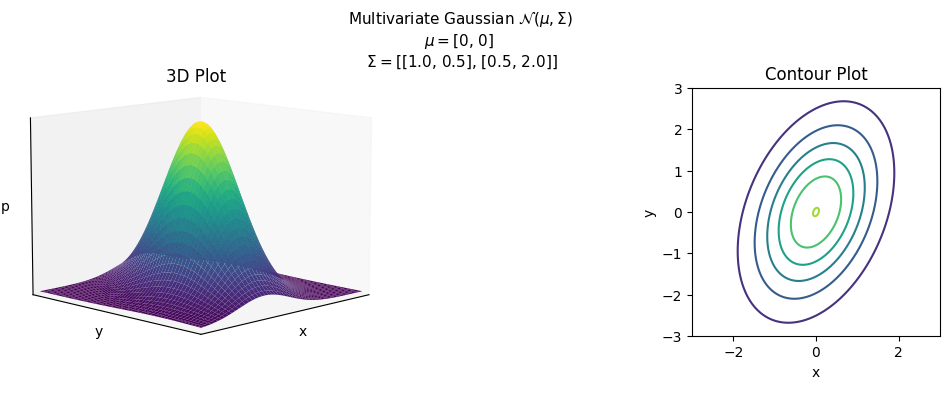
\includegraphics{notebooks/basic-math_files/figure-pdf/cell-11-output-1.png}

}

\end{figure}

\begin{Shaded}
\begin{Highlighting}[]
\NormalTok{x }\OperatorTok{=}\NormalTok{ np.arange(}\OperatorTok{{-}}\DecValTok{10}\NormalTok{, }\DecValTok{10}\NormalTok{, }\FloatTok{0.1}\NormalTok{)}
\NormalTok{f }\OperatorTok{=} \KeywordTok{lambda}\NormalTok{ x: }\DecValTok{2} \OperatorTok{*}\NormalTok{ x}
\NormalTok{plot\_function(x, f, xlim}\OperatorTok{=}\NormalTok{(}\OperatorTok{{-}}\DecValTok{5}\NormalTok{, }\DecValTok{5}\NormalTok{), ylim}\OperatorTok{=}\NormalTok{(}\OperatorTok{{-}}\DecValTok{5}\NormalTok{, }\DecValTok{5}\NormalTok{), ticks\_every}\OperatorTok{=}\NormalTok{[}\DecValTok{1}\NormalTok{, }\DecValTok{1}\NormalTok{], }
\NormalTok{              title}\OperatorTok{=}\StringTok{\textquotesingle{}Linear Function: $y=2x$\textquotesingle{}}\NormalTok{)}
\end{Highlighting}
\end{Shaded}

\begin{figure}[H]

{\centering 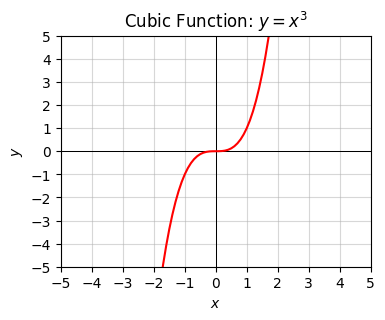
\includegraphics{notebooks/basic-math_files/figure-pdf/cell-12-output-1.png}

}

\end{figure}

\begin{Shaded}
\begin{Highlighting}[]
\NormalTok{x }\OperatorTok{=}\NormalTok{ np.arange(}\OperatorTok{{-}}\DecValTok{10}\NormalTok{, }\DecValTok{10}\NormalTok{, }\FloatTok{0.1}\NormalTok{)}
\NormalTok{f }\OperatorTok{=} \KeywordTok{lambda}\NormalTok{ x: }\DecValTok{2} \OperatorTok{*}\NormalTok{ x }\OperatorTok{{-}} \DecValTok{1}
\NormalTok{plot\_function(x, f, xlim}\OperatorTok{=}\NormalTok{(}\OperatorTok{{-}}\DecValTok{5}\NormalTok{, }\DecValTok{5}\NormalTok{), ylim}\OperatorTok{=}\NormalTok{(}\OperatorTok{{-}}\DecValTok{5}\NormalTok{, }\DecValTok{5}\NormalTok{), ticks\_every}\OperatorTok{=}\NormalTok{[}\DecValTok{1}\NormalTok{, }\DecValTok{1}\NormalTok{], }
\NormalTok{              title}\OperatorTok{=}\StringTok{\textquotesingle{}Affine Function: $y=2x{-}1$\textquotesingle{}}\NormalTok{)}
\end{Highlighting}
\end{Shaded}

\begin{figure}[H]

{\centering \includegraphics{notebooks/basic-math_files/figure-pdf/cell-13-output-1.png}

}

\end{figure}

\hypertarget{polynomial-functions}{%
\subsection{Polynomial Functions}\label{polynomial-functions}}

Polynomial functions are just sums of positive integer powers of \(x\),
e.g.~something like \(y=3x^2+5x+1\) or \(y=x^{10}-x^{3}+4\). The highest
power that shows up in the function is called the \textbf{degree} of the
polynomial. For example, the above examples have degrees 2 and 10
respectively. Polynomial functions tend to look like lines, bowls, or
roller coasters that turn up and down some number of times.

A major example is the quadratic function \(y=x^2\), which is just an
upward-shaped bowl. Its bowl-shaped curve is called a \textbf{parabola}.
We can get a downward-shaped bowl by flipping the sign to \(y=-x^2\).

\begin{Shaded}
\begin{Highlighting}[]
\NormalTok{x }\OperatorTok{=}\NormalTok{ np.arange(}\OperatorTok{{-}}\DecValTok{10}\NormalTok{, }\DecValTok{10}\NormalTok{, }\FloatTok{0.1}\NormalTok{)}
\NormalTok{f }\OperatorTok{=} \KeywordTok{lambda}\NormalTok{ x: x }\OperatorTok{**} \DecValTok{2}
\NormalTok{plot\_function(x, f, xlim}\OperatorTok{=}\NormalTok{(}\OperatorTok{{-}}\DecValTok{5}\NormalTok{, }\DecValTok{5}\NormalTok{), ylim}\OperatorTok{=}\NormalTok{(}\DecValTok{0}\NormalTok{, }\DecValTok{10}\NormalTok{), ticks\_every}\OperatorTok{=}\NormalTok{[}\DecValTok{1}\NormalTok{, }\DecValTok{1}\NormalTok{], }
\NormalTok{              title}\OperatorTok{=}\StringTok{\textquotesingle{}Quadratic Function: $y=x\^{}2$\textquotesingle{}}\NormalTok{)}
\end{Highlighting}
\end{Shaded}

\begin{figure}[H]

{\centering 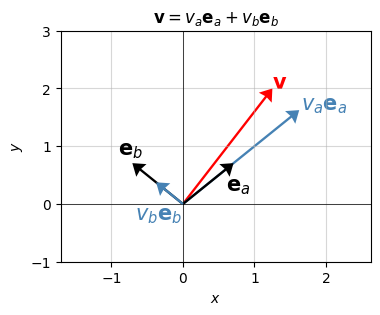
\includegraphics{notebooks/basic-math_files/figure-pdf/cell-14-output-1.png}

}

\end{figure}

The next one up is the cubic function \(y=x^3\). The cubic looks
completely different from the bowl-shaped parabola.

\begin{Shaded}
\begin{Highlighting}[]
\NormalTok{x }\OperatorTok{=}\NormalTok{ np.arange(}\OperatorTok{{-}}\DecValTok{10}\NormalTok{, }\DecValTok{10}\NormalTok{, }\FloatTok{0.1}\NormalTok{)}
\NormalTok{f }\OperatorTok{=} \KeywordTok{lambda}\NormalTok{ x: x }\OperatorTok{**} \DecValTok{3}
\NormalTok{plot\_function(x, f, xlim}\OperatorTok{=}\NormalTok{(}\OperatorTok{{-}}\DecValTok{5}\NormalTok{, }\DecValTok{5}\NormalTok{), ylim}\OperatorTok{=}\NormalTok{(}\OperatorTok{{-}}\DecValTok{5}\NormalTok{, }\DecValTok{5}\NormalTok{), ticks\_every}\OperatorTok{=}\NormalTok{[}\DecValTok{1}\NormalTok{, }\DecValTok{1}\NormalTok{], }
\NormalTok{              title}\OperatorTok{=}\StringTok{\textquotesingle{}Cubic Function: $y=x\^{}3$\textquotesingle{}}\NormalTok{)}
\end{Highlighting}
\end{Shaded}

\begin{figure}[H]

{\centering 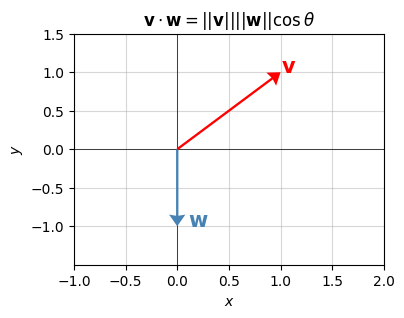
\includegraphics{notebooks/basic-math_files/figure-pdf/cell-15-output-1.png}

}

\end{figure}

Polynomials can take on much more interesting shapes than this. Here's a
more interesting polynomial degree 10,

\[y = (x^2 - 1)^5 - 5(x^2 - 1)^4 + 10(x^2 - 1)^3 - 10(x^2 - 1)^2 + 5(x^2 - 1) - 1.\]

\begin{Shaded}
\begin{Highlighting}[]
\NormalTok{x }\OperatorTok{=}\NormalTok{ np.arange(}\OperatorTok{{-}}\DecValTok{10}\NormalTok{, }\DecValTok{10}\NormalTok{, }\FloatTok{0.1}\NormalTok{)}
\KeywordTok{def}\NormalTok{ f(x): }
\NormalTok{    y }\OperatorTok{=}\NormalTok{ (x}\OperatorTok{**}\DecValTok{2} \OperatorTok{{-}} \DecValTok{1}\NormalTok{)}\OperatorTok{**}\DecValTok{5} \OperatorTok{{-}} \DecValTok{5} \OperatorTok{*}\NormalTok{ (x}\OperatorTok{**}\DecValTok{2} \OperatorTok{{-}} \DecValTok{1}\NormalTok{)}\OperatorTok{**}\DecValTok{4} \OperatorTok{+} \DecValTok{10} \OperatorTok{*}\NormalTok{ (x}\OperatorTok{**}\DecValTok{2} \OperatorTok{{-}} \DecValTok{1}\NormalTok{)}\OperatorTok{**}\DecValTok{3} \OperatorTok{{-}} 
    \DecValTok{10} \OperatorTok{*}\NormalTok{ (x}\OperatorTok{**}\DecValTok{2} \OperatorTok{{-}} \DecValTok{1}\NormalTok{)}\OperatorTok{**}\DecValTok{2} \OperatorTok{+} \DecValTok{5} \OperatorTok{*}\NormalTok{ (x}\OperatorTok{**}\DecValTok{2} \OperatorTok{{-}} \DecValTok{1}\NormalTok{) }\OperatorTok{{-}} \DecValTok{1}
\NormalTok{plot\_function(x, f, xlim}\OperatorTok{=}\NormalTok{(}\OperatorTok{{-}}\DecValTok{3}\NormalTok{, }\DecValTok{3}\NormalTok{), ylim}\OperatorTok{=}\NormalTok{(}\OperatorTok{{-}}\DecValTok{40}\NormalTok{, }\DecValTok{40}\NormalTok{), ticks\_every}\OperatorTok{=}\NormalTok{[}\DecValTok{1}\NormalTok{, }\DecValTok{10}\NormalTok{], }
\NormalTok{              title}\OperatorTok{=}\StringTok{\textquotesingle{}Arbitrary Polynomial\textquotesingle{}}\NormalTok{)}
\end{Highlighting}
\end{Shaded}

\begin{figure}[H]

{\centering \includegraphics{notebooks/basic-math_files/figure-pdf/cell-16-output-1.png}

}

\end{figure}

\hypertarget{rational-functions}{%
\subsection{Rational Functions}\label{rational-functions}}

Rational functions are functions that are ratios of polynomial
functions. Examples might be \(y=\frac{1}{x}\), or

\[y=\frac{x^3+x+1}{x^2-1}.\]

These functions typically look kind of like polynomial functions, but
have points where the curve ``blows up'' to positive or negative
infinity. The points where the function blows up are called
\textbf{poles} or \textbf{asymptotes}.

Here's a plot of the function

\[y=\frac{x^3+x+1}{x^2-1}.\]

Notice how weird it looks. There are asymptotes (the vertical lines)
where the function blows up at \(\pm 1\), which is where the denominator
\(x^2-1=0\).

\begin{Shaded}
\begin{Highlighting}[]
\NormalTok{x }\OperatorTok{=}\NormalTok{ np.arange(}\OperatorTok{{-}}\DecValTok{10}\NormalTok{, }\DecValTok{10}\NormalTok{, }\FloatTok{0.01}\NormalTok{)}
\NormalTok{f }\OperatorTok{=} \KeywordTok{lambda}\NormalTok{ x: (x }\OperatorTok{**} \DecValTok{3} \OperatorTok{+}\NormalTok{ x }\OperatorTok{+} \DecValTok{1}\NormalTok{) }\OperatorTok{/}\NormalTok{ (x }\OperatorTok{**} \DecValTok{2} \OperatorTok{{-}} \DecValTok{1}\NormalTok{)}
\NormalTok{plot\_function(x, f, xlim}\OperatorTok{=}\NormalTok{(}\OperatorTok{{-}}\DecValTok{5}\NormalTok{, }\DecValTok{5}\NormalTok{), ylim}\OperatorTok{=}\NormalTok{(}\OperatorTok{{-}}\DecValTok{5}\NormalTok{, }\DecValTok{5}\NormalTok{), ticks\_every}\OperatorTok{=}\NormalTok{[}\DecValTok{1}\NormalTok{, }\DecValTok{1}\NormalTok{], }
\NormalTok{              title}\OperatorTok{=}\StringTok{\textquotesingle{}Rational Function\textquotesingle{}}\NormalTok{)}
\end{Highlighting}
\end{Shaded}

\begin{figure}[H]

{\centering \includegraphics{notebooks/basic-math_files/figure-pdf/cell-17-output-1.png}

}

\end{figure}

Here's a plot of \(y=\frac{1}{x}\). There's an asymptote at \(x=0\).
When \(x > 0\) it starts at \(+\infty\) and tapers down to \(0\) as
\(x\) gets large. When \(x < 0\) it does the same thing, except flipped
across the origin \(x=y=0\). This is an example of an \textbf{odd
function}, a function that looks like \(f(x)=-f(x)\), which is clear in
this case since \(1/(-x)=-1/x\). Functions like the linear function
\(y=x\) and the cubic function \(y=x^3\) are also odd functions.

\begin{Shaded}
\begin{Highlighting}[]
\NormalTok{x }\OperatorTok{=}\NormalTok{ np.arange(}\OperatorTok{{-}}\DecValTok{10}\NormalTok{, }\DecValTok{10}\NormalTok{, }\FloatTok{0.1}\NormalTok{)}
\NormalTok{f }\OperatorTok{=} \KeywordTok{lambda}\NormalTok{ x: }\DecValTok{1} \OperatorTok{/}\NormalTok{ x}
\NormalTok{plot\_function(x, f, xlim}\OperatorTok{=}\NormalTok{(}\OperatorTok{{-}}\DecValTok{5}\NormalTok{, }\DecValTok{5}\NormalTok{), ylim}\OperatorTok{=}\NormalTok{(}\OperatorTok{{-}}\DecValTok{5}\NormalTok{, }\DecValTok{5}\NormalTok{), ticks\_every}\OperatorTok{=}\NormalTok{[}\DecValTok{1}\NormalTok{, }\DecValTok{1}\NormalTok{], }
\NormalTok{              title}\OperatorTok{=}\StringTok{\textquotesingle{}Odd Function: $y=1/x$\textquotesingle{}}\NormalTok{)}
\end{Highlighting}
\end{Shaded}

\begin{figure}[H]

{\centering \includegraphics{notebooks/basic-math_files/figure-pdf/cell-18-output-1.png}

}

\end{figure}

A related function is \(y=\frac{1}{|x|}\). The difference here is that
\(|x|\) can never be negative. This means \(f(x)=f(-x)\). This is called
an \textbf{even function}. Functions like this are symmetric across the
y-axis. The quadratic function \(y=x^2\) is also an even function.

\begin{Shaded}
\begin{Highlighting}[]
\NormalTok{x }\OperatorTok{=}\NormalTok{ np.arange(}\OperatorTok{{-}}\DecValTok{10}\NormalTok{, }\DecValTok{10}\NormalTok{, }\FloatTok{0.1}\NormalTok{)}
\NormalTok{f }\OperatorTok{=} \KeywordTok{lambda}\NormalTok{ x: }\DecValTok{1} \OperatorTok{/}\NormalTok{ np.}\BuiltInTok{abs}\NormalTok{(x)}
\NormalTok{plot\_function(x, f, xlim}\OperatorTok{=}\NormalTok{(}\OperatorTok{{-}}\DecValTok{5}\NormalTok{, }\DecValTok{5}\NormalTok{), ylim}\OperatorTok{=}\NormalTok{(}\OperatorTok{{-}}\DecValTok{1}\NormalTok{, }\DecValTok{5}\NormalTok{), ticks\_every}\OperatorTok{=}\NormalTok{[}\DecValTok{1}\NormalTok{, }\DecValTok{1}\NormalTok{], }
\NormalTok{              title}\OperatorTok{=}\StringTok{\textquotesingle{}Even Function: $y=1/|x|$\textquotesingle{}}\NormalTok{)}
\end{Highlighting}
\end{Shaded}

\begin{figure}[H]

{\centering \includegraphics{notebooks/basic-math_files/figure-pdf/cell-19-output-1.png}

}

\end{figure}

\hypertarget{power-functions}{%
\subsection{Power Functions}\label{power-functions}}

Functions that look like \(y=\frac{1}{x^n}\) for some \(n\) are
sometimes called inverse, hyperbolic. These can be represented more
easily by using a negative power like \(y=x^{-n}\), which means the
exact same thing as \(y=\frac{1}{x^n}\).

We can extend \(n\) to deal with things like square roots or cube roots
or any kind of root as well by allowing \(n\) to be non-integer. For
example, we can represent the square root function \(y=\sqrt{x}\) as
\(y=x^{1/2}\), and the cube root \(y=\sqrt[3]{x}\) as \(y=x^{1/3}\).
Roots like these are only defined when \(x \geq 0\).

The general class of functions of the form \(y=x^p\) for some arbitrary
real number \(p\) are often called \textbf{power functions}.

Here's a plot of what the square root function looks like. Here \(y\)
grows slower than a linear function, but still grows arbitrarily large
with \(x\).

\begin{Shaded}
\begin{Highlighting}[]
\NormalTok{x }\OperatorTok{=}\NormalTok{ np.arange(}\DecValTok{0}\NormalTok{, }\DecValTok{10}\NormalTok{, }\FloatTok{0.1}\NormalTok{)}
\NormalTok{f }\OperatorTok{=} \KeywordTok{lambda}\NormalTok{ x: np.sqrt(x)}
\NormalTok{plot\_function(x, f, xlim}\OperatorTok{=}\NormalTok{(}\DecValTok{0}\NormalTok{, }\DecValTok{5}\NormalTok{), ylim}\OperatorTok{=}\NormalTok{(}\OperatorTok{{-}}\DecValTok{2}\NormalTok{, }\DecValTok{4}\NormalTok{), ticks\_every}\OperatorTok{=}\NormalTok{[}\DecValTok{1}\NormalTok{, }\DecValTok{1}\NormalTok{], }
\NormalTok{              title}\OperatorTok{=}\StringTok{\textquotesingle{}Square Root: $y=\textbackslash{}sqrt}\SpecialCharTok{\{x\}}\StringTok{=x\^{}\{1/2\}$\textquotesingle{}}\NormalTok{)}
\end{Highlighting}
\end{Shaded}

\begin{figure}[H]

{\centering 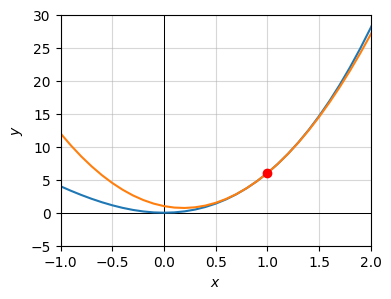
\includegraphics{notebooks/basic-math_files/figure-pdf/cell-20-output-1.png}

}

\end{figure}

Power functions obey the following rules:

\begin{longtable}[]{@{}
  >{\raggedright\arraybackslash}p{(\columnwidth - 2\tabcolsep) * \real{0.4878}}
  >{\raggedright\arraybackslash}p{(\columnwidth - 2\tabcolsep) * \real{0.5122}}@{}}
\toprule()
\endhead
\textbf{Rule} & \textbf{Example} \\
\(x^0 = 1\) & \(2^0 = 1\) \\
\(x^{m+n} = x^m x^n\) & \(3^{2+5} = 3^2 3^5 = 3^8 = 6561\) \\
\(x^{m-n} = \frac{x^m}{x^n}\) &
\(3^{2-5} = \frac{3^2}{3^5} = 3^{-3} \approx 0.037\) \\
\(x^{mn} = (x^m)^n\) & \(2^{2 \cdot 5} = (2^2)^5 = 2^{10} = 1024\) \\
\((xy)^n = x^n y^n\) & \((2 \cdot 2)^3 = 2^3 2^3 = 4^3 = 2^6 = 64\) \\
\(\big(\frac{x}{y}\big)^n = \frac{x^n}{y^n}\) &
\(\big(\frac{2}{4}\big)^3 = \frac{2^3}{4^3} = \frac{1}{8}\) \\
\(\big(\frac{x}{y}\big)^{-n} = \frac{y^n}{x^n}\) &
\(\big(\frac{2}{4}\big)^{-3} = \frac{4^3}{2^3} = 2^3 = 8\) \\
\(x^{1/2} = \sqrt{x} = \sqrt[2]{x}\) & \(4^{1/2} = \sqrt{4} = 2\) \\
\(x^{1/n} = \sqrt[n]{x}\) & \(3^{1/4} = \sqrt[4]{3} \approx 1.316\) \\
\(x^{m/n} = \sqrt[n]{x^m}\) &
\(3^{3/4} = \sqrt[4]{3^3} = \sqrt[4]{9} \approx 1.732\) \\
\(\sqrt[n]{xy} = \sqrt[n]{x} \sqrt[n]{y}\) &
\(\sqrt[4]{3 \cdot 2} = \sqrt[4]{3} \sqrt[4]{2} \approx 1.565\) \\
\(\sqrt[n]{\frac{x}{y}} = \frac{\sqrt[n]{x}}{\sqrt[n]{y}}\) &
\(\sqrt[4]{\frac{3}{2}} = \frac{\sqrt[4]{3}}{\sqrt[4]{2}} \approx 1.107\) \\
\bottomrule()
\end{longtable}

It's important to remember that power functions \emph{do not} distribute
over addition, i.e.

\[(x+y)^n \neq x^n + y^n,\]

and by extension nor do roots,

\[\sqrt[n]{x+y} \neq \sqrt[n]{x} + \sqrt[n]{y}.\]

\hypertarget{exponentials-and-logarithms}{%
\subsection{Exponentials and
Logarithms}\label{exponentials-and-logarithms}}

Two very important functions are the exponential function \(y=\exp(x)\)
and the logarithm function \(y=\log(x)\). They show up surprisingly
often in machine learning and the sciences, certainly more than most
other special functions do.

The exponential function can be written as a power by defining a number
\(e\) called Euler's number, given by \(e = 2.71828\dots\) . Like
\(\pi\), \(e\) is an example of an irrational number, i.e.~a number that
can't be represented as a ratio of integers. Using \(e\), we can write
the exponential function in the more usual form \(y=e^x\), where it's
roughly speaking understood that we mean ``multiply \(e\) by itself
\(x\) times''. For example, \(\exp(2) = e^2 = e \cdot e\).

The logarithm is defined as the inverse of the exponential function.
It's the unique function satisfying \(\log(\exp(x)) = x\). The opposite
is also true since the exponential must then be the inverse of the
logarithm function, \(\exp(\log(x)) = x\). This gives a way of mapping
between the two functions,

\[\log(a) = b \quad \Longleftrightarrow \quad \exp(b) = a.\]

Here are some plots of what the exponential and logarithm functions look
like. The exponential function is a function that blows up very, very
quickly. The log function grows very, very slowly (much more slowly than
the square root does).

Note the log function is only defined for positive-valued numbers
\(x \geq 0\), with \(\log(+0)=-\infty\). This is dual to the exponential
function only taking on \(y \geq 0\).

\begin{Shaded}
\begin{Highlighting}[]
\NormalTok{x }\OperatorTok{=}\NormalTok{ np.arange(}\OperatorTok{{-}}\DecValTok{5}\NormalTok{, }\DecValTok{5}\NormalTok{, }\FloatTok{0.1}\NormalTok{)}
\NormalTok{f }\OperatorTok{=} \KeywordTok{lambda}\NormalTok{ x: np.exp(x)}
\NormalTok{plot\_function(x, f, xlim}\OperatorTok{=}\NormalTok{(}\OperatorTok{{-}}\DecValTok{5}\NormalTok{, }\DecValTok{5}\NormalTok{), ylim}\OperatorTok{=}\NormalTok{(}\OperatorTok{{-}}\DecValTok{1}\NormalTok{, }\DecValTok{10}\NormalTok{), ticks\_every}\OperatorTok{=}\NormalTok{[}\DecValTok{1}\NormalTok{, }\DecValTok{2}\NormalTok{], }
\NormalTok{              title}\OperatorTok{=}\StringTok{\textquotesingle{}Exponential Function: $y=\textbackslash{}exp(x)$\textquotesingle{}}\NormalTok{)}
\end{Highlighting}
\end{Shaded}

\begin{figure}[H]

{\centering 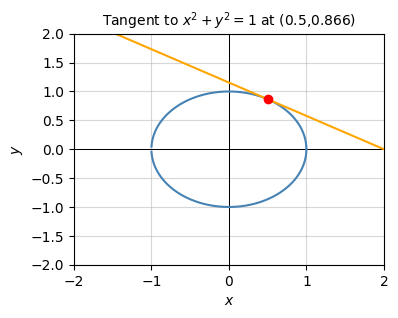
\includegraphics{notebooks/basic-math_files/figure-pdf/cell-21-output-1.png}

}

\end{figure}

\begin{Shaded}
\begin{Highlighting}[]
\NormalTok{x }\OperatorTok{=}\NormalTok{ np.arange(}\FloatTok{0.01}\NormalTok{, }\DecValTok{5}\NormalTok{, }\FloatTok{0.1}\NormalTok{)}
\NormalTok{f }\OperatorTok{=} \KeywordTok{lambda}\NormalTok{ x: np.log(x)}
\NormalTok{plot\_function(x, f, xlim}\OperatorTok{=}\NormalTok{(}\OperatorTok{{-}}\DecValTok{1}\NormalTok{, }\DecValTok{5}\NormalTok{), ylim}\OperatorTok{=}\NormalTok{(}\OperatorTok{{-}}\DecValTok{5}\NormalTok{, }\DecValTok{2}\NormalTok{), ticks\_every}\OperatorTok{=}\NormalTok{[}\DecValTok{1}\NormalTok{, }\DecValTok{1}\NormalTok{], }
\NormalTok{              title}\OperatorTok{=}\StringTok{\textquotesingle{}Logarithm Function: $y=\textbackslash{}log(x)$\textquotesingle{}}\NormalTok{)}
\end{Highlighting}
\end{Shaded}

\begin{figure}[H]

{\centering \includegraphics{notebooks/basic-math_files/figure-pdf/cell-22-output-1.png}

}

\end{figure}

The exponential and logarithm functions I defined are the ``natural''
way to define these functions. We can also have exponential functions in
other bases, \(y=a^x\) for any positive number \(a\). Each \(a\) has an
equivalent logarithm, written \(y = \log_{a}(x)\). The two functions
\(y=a^x\) and \(y=\log_{a}(x)\) are inverses of each other. When I leave
off the \(a\), it's assumed that all logs are the natural base \(a=e\),
sometimes also written \(\ln(x)\).

Two common examples of other bases that show up sometimes are the base-2
functions \(2^x\) and \(\log_{2}(x)\), and the base-10 functions
\(10^x\) and \(\log_{10}(x)\). Base-2 functions in particular show up
often in computer science because of the tendency to think in bits.
Base-10 functions show up when we want to think about how many digits a
number has.

Here are some rules that exponentials and logs obey:

\begin{longtable}[]{@{}
  >{\raggedright\arraybackslash}p{(\columnwidth - 2\tabcolsep) * \real{0.4878}}
  >{\raggedright\arraybackslash}p{(\columnwidth - 2\tabcolsep) * \real{0.5122}}@{}}
\toprule()
\endhead
\textbf{Rule} & \textbf{Example} \\
\(e^0 = 1\) & \\
\(\log(1) = 0\) & \\
\(\log(e) = 1\) & \\
\(e^{a+b} = e^a e^b\) & \(e^{2+5} = e^2 e^5 = e^8 \approx 2980.96\) \\
\(e^{a-b} = \frac{e^a}{e^b}\) &
\(e^{2-5} = \frac{e^2}{e^5} = e^{-3} \approx 0.0498\) \\
\(e^{ab} = (e^a)^b\) &
\(e^{2 \cdot 5} = (e^2)^5 = e^{10} \approx 22026.47\) \\
\(a^b = e^{b \log(a)}\) & \(2^3 = e^{3 \log(2)} = 8\) \\
\(\log(ab) = \log(a) + \log(b)\) &
\(\log(2 \cdot 5) = \log(2) + \log(5) = \log(10) \approx 2.303\) \\
\(\log\big(\frac{a}{b}\big) = \log(a) - \log(b)\) &
\(\log\big(\frac{2}{5}\big) = \log(2) - \log(5) \approx -0.916\) \\
\(\log(a^b) = b\log(a)\) & \(\log(5^2) = 2\log(5) \approx 3.219\) \\
\(\log_a(x) = \frac{\log(x)}{\log(a)}\) &
\(\log_2(5) = \frac{\log(5)}{\log(2)} \approx 2.322\) \\
\bottomrule()
\end{longtable}

Here's an example of an equation involving exponentials and logs.
Suppose you have \(n\) bits of numbers (perhaps it's the precision in
some float) and you want to know how many \emph{digits} this number
takes up in decimal form (what you're used to). This would be equivalent
to solving the following equation for \(x\),

\begin{align*}
2^n &= 10^{x} \\
\log(2^n) &= \log(10^{x}) \\
n\log(2) &= x\log(10) \\
x &= \frac{\log(2)}{\log(10)} \cdot n \\
x &\approx 0.3 \cdot n. \\
\end{align*}

For example, you can use this formula to show that 52 bits of floating
point precision translates to about 15 to 16 digits of precision. In
numpy, the function \texttt{np.log} function calculates the (base-\(e\))
log of a number.

\begin{Shaded}
\begin{Highlighting}[]
\NormalTok{n }\OperatorTok{=} \DecValTok{52}
\NormalTok{x }\OperatorTok{=}\NormalTok{ np.log(}\DecValTok{2}\NormalTok{) }\OperatorTok{/}\NormalTok{ np.log(}\DecValTok{10}\NormalTok{) }\OperatorTok{*}\NormalTok{ n}
\BuiltInTok{print}\NormalTok{(}\SpecialStringTok{f\textquotesingle{}x = }\SpecialCharTok{\{}\NormalTok{x}\SpecialCharTok{\}}\SpecialStringTok{\textquotesingle{}}\NormalTok{)}
\end{Highlighting}
\end{Shaded}

\begin{verbatim}
x = 15.65355977452702
\end{verbatim}

\hypertarget{trigonometric-functions}{%
\subsection{Trigonometric Functions}\label{trigonometric-functions}}

Other textbook functions typically covered in math courses are the trig
functions: sine, cosine, tangent, cosine, cosecant, and cotangent. Of
these functions, the most important to know are the sine function
\(y=\sin x\), the cosine function \(y = \cos x\), and \emph{sometimes}
the tangent function \(y = \tan x\).

Here's what their plots look like. They're both waves that repeat
themselves, in the sense \(f(x + 2\pi) = f(x)\). The length for the
function to repeat itself is called the \emph{period}, in this case
\(2\pi \approx 6.28\). Note that the cosine is just a sine function
that's shifted right by \(\frac{\pi}{2} \approx 1.57\).

\begin{Shaded}
\begin{Highlighting}[]
\NormalTok{x }\OperatorTok{=}\NormalTok{ np.arange(}\OperatorTok{{-}}\DecValTok{10}\NormalTok{, }\DecValTok{10}\NormalTok{, }\FloatTok{0.1}\NormalTok{)}
\NormalTok{f }\OperatorTok{=} \KeywordTok{lambda}\NormalTok{ x: np.sin(x)}
\NormalTok{plot\_function(x, f, xlim}\OperatorTok{=}\NormalTok{(}\OperatorTok{{-}}\DecValTok{6}\NormalTok{, }\DecValTok{6}\NormalTok{), ylim}\OperatorTok{=}\NormalTok{(}\OperatorTok{{-}}\DecValTok{2}\NormalTok{, }\DecValTok{2}\NormalTok{),  ticks\_every}\OperatorTok{=}\NormalTok{[}\DecValTok{1}\NormalTok{, }\FloatTok{0.5}\NormalTok{], }
\NormalTok{              title}\OperatorTok{=}\StringTok{\textquotesingle{}Sine Function: $y=\textbackslash{}sin(x)$\textquotesingle{}}\NormalTok{)}
\end{Highlighting}
\end{Shaded}

\begin{figure}[H]

{\centering 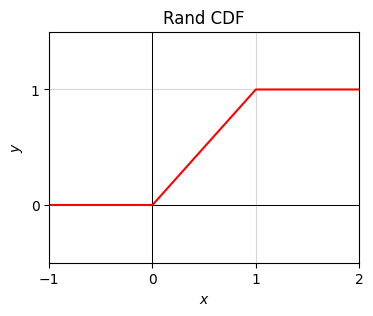
\includegraphics{notebooks/basic-math_files/figure-pdf/cell-24-output-1.png}

}

\end{figure}

\begin{Shaded}
\begin{Highlighting}[]
\NormalTok{x }\OperatorTok{=}\NormalTok{ np.arange(}\OperatorTok{{-}}\DecValTok{10}\NormalTok{, }\DecValTok{10}\NormalTok{, }\FloatTok{0.1}\NormalTok{)}
\NormalTok{f }\OperatorTok{=} \KeywordTok{lambda}\NormalTok{ x: np.cos(x)}
\NormalTok{plot\_function(x, f, xlim}\OperatorTok{=}\NormalTok{(}\OperatorTok{{-}}\DecValTok{6}\NormalTok{, }\DecValTok{6}\NormalTok{), ylim}\OperatorTok{=}\NormalTok{(}\OperatorTok{{-}}\DecValTok{2}\NormalTok{, }\DecValTok{2}\NormalTok{), ticks\_every}\OperatorTok{=}\NormalTok{[}\DecValTok{1}\NormalTok{, }\FloatTok{0.5}\NormalTok{], }
\NormalTok{              title}\OperatorTok{=}\StringTok{\textquotesingle{}Cosine Function: $y=\textbackslash{}cos(x)$\textquotesingle{}}\NormalTok{)}
\end{Highlighting}
\end{Shaded}

\begin{figure}[H]

{\centering \includegraphics{notebooks/basic-math_files/figure-pdf/cell-25-output-1.png}

}

\end{figure}

Trig functions don't really show up that much in machine learning, so I
won't remind you of all those obscure trig rules you've forgotten. I'll
just mention that we can define all the other trig functions using the
sine and cosine as follows,

\begin{align*}
&\tan x = \frac{\sin x}{\cos x}, \\
&\csc x = \frac{1}{\sin x}, \\
&\sec x = \frac{1}{\cos x}, \\
&\cot x = \frac{1}{\tan x} = \frac{\cos x}{\sin x}.
\end{align*}

We can talk about the \emph{inverse} of trig functions as well. These
are just the functions that undo the trig operations and give you back
the angle (in radians). Since none of the trig functions are monotonic,
we can't invert them on the whole real line, but only on a given range.

Below I'll just list the inverse sine, cosine, and tangent functions and
their defined input and output ranges. Note by historical convention,
these inverse functions are usually called the \textbf{arcsine},
\textbf{arccosine}, and \textbf{arctangent} respectfully.

\begin{longtable}[]{@{}
  >{\raggedright\arraybackslash}p{(\columnwidth - 4\tabcolsep) * \real{0.3226}}
  >{\raggedright\arraybackslash}p{(\columnwidth - 4\tabcolsep) * \real{0.3387}}
  >{\raggedright\arraybackslash}p{(\columnwidth - 4\tabcolsep) * \real{0.3387}}@{}}
\toprule()
\endhead
\textbf{Inverse Function} & \textbf{Input Range} & \textbf{Output
Range} \\
\(y = \arcsin x = \sin^{-1} x\) & \(-1 \leq x \leq 1\) &
\(-90^\circ \leq y \leq 90^\circ\) \\
\(y = \arccos x = \cos^{-1} x\) & \(-1 \leq x \leq 1\) &
\(0^\circ \leq y \leq 180^\circ\) \\
\(y = \arctan x = \tan^{-1} x\) & \(-\infty < x < \infty\) &
\(-90^\circ \leq y \leq 90^\circ\) \\
\bottomrule()
\end{longtable}

\hypertarget{piecewise-functions}{%
\subsection{Piecewise Functions}\label{piecewise-functions}}

The functions covered so far are examples of \textbf{continuous
functions}. Their graphs don't have jumps or holes in them anywhere.
Continuous functions we can often write using a single equation, like
\(y=x^2\) or \(y=1 + \sin(x)\). We can also have functions that require
more than one equation to write. These are called \textbf{piecewise
functions}. Piecewise functions usually aren't continuous, but sometimes
can be.

An example of a discontinuous piecewise function is the unit step
function \(y=u(x)\) given by

\[
y = 
\begin{cases}
0 & x < 0, \\
1 & x \geq 0.
\end{cases}
\]

This expression means \(y=0\) whenever \(x < 0\), but \(y=1\) whenever
\(x \geq 0\). It breaks up into two pieces, one horizontal line \(y=0\)
when \(x\) is negative, and another horizontal line \(y=1\) when \(x\)
is positive.

Using Boolean expressions, we can also write this function in a more
economical way by agreeing to identify \(x=1\) with \(\text{TRUE}\) and
\(x=0\) with \(\text{FALSE}\), which python does by default. In this
notation, we can write

\[u(x) = [x \geq 0],\]

which means exactly the same thing as the piecewise definition, since
\(x \geq 0\) is only true when (you guessed it), \(x \geq 0\).

Here's a plot of this function. Note the discontinuous jump at \(x=0\).

\begin{Shaded}
\begin{Highlighting}[]
\NormalTok{x }\OperatorTok{=}\NormalTok{ np.arange(}\OperatorTok{{-}}\DecValTok{10}\NormalTok{, }\DecValTok{10}\NormalTok{, }\FloatTok{0.01}\NormalTok{)}
\NormalTok{f }\OperatorTok{=} \KeywordTok{lambda}\NormalTok{ x:  (x }\OperatorTok{\textgreater{}=} \DecValTok{0}\NormalTok{)}
\NormalTok{plot\_function(x, f, xlim}\OperatorTok{=}\NormalTok{(}\OperatorTok{{-}}\DecValTok{3}\NormalTok{, }\DecValTok{3}\NormalTok{), ylim}\OperatorTok{=}\NormalTok{(}\OperatorTok{{-}}\DecValTok{1}\NormalTok{, }\DecValTok{2}\NormalTok{), ticks\_every}\OperatorTok{=}\NormalTok{[}\DecValTok{1}\NormalTok{, }\FloatTok{0.5}\NormalTok{], }
\NormalTok{              title}\OperatorTok{=}\StringTok{\textquotesingle{}Unit Step Function: $y=u(x)$\textquotesingle{}}\NormalTok{)}
\end{Highlighting}
\end{Shaded}

\begin{figure}[H]

{\centering 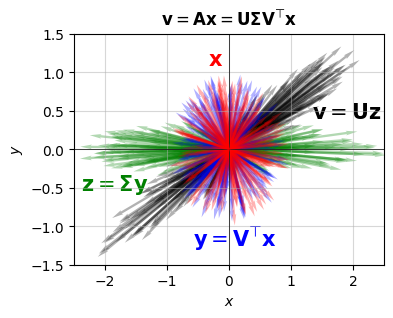
\includegraphics{notebooks/basic-math_files/figure-pdf/cell-26-output-1.png}

}

\end{figure}

An example of a piecewise function that's continuous is the \textbf{ramp
function}, defined by

\[
y = 
\begin{cases}
0 & x < 0, \\
x & x \geq 0.
\end{cases}
\]

This function gives a horizontal line \(y=0\) when \(x\) is negative,
and a \(45^\circ\) line \(y=x\) when \(x\) is positive. Both lines
connect at \(x=0\), but leave a kink in the graph.

Another way to write the same thing using Boolean expressions is
\(y = x \cdot [x \geq 0]\), which is of course just
\(y = x \cdot u(x)\).

In machine learning it's more common to write the ramp function using
the \(\max\) function as \(y = \max(0,x)\). This means, for each \(x\),
take that value and compare it with \(0\), and take the maximum of those
two. That is, if \(x\) is negative take \(y=0\), otherwise take \(y=x\).
It's also more common to call this function a \textbf{rectified linear
unit}, or \textbf{ReLU} for short. It's an ugly, unintuitive name, but
unfortunately it's stuck in the field.

Here's a plot of the ramp or ReLU function. Notice how it stays at
\(y=0\) for a while, then suddenly ``ramps upward'' at \(x=0\).

\begin{Shaded}
\begin{Highlighting}[]
\NormalTok{x }\OperatorTok{=}\NormalTok{ np.arange(}\OperatorTok{{-}}\DecValTok{10}\NormalTok{, }\DecValTok{10}\NormalTok{, }\FloatTok{0.1}\NormalTok{)}
\NormalTok{f }\OperatorTok{=} \KeywordTok{lambda}\NormalTok{ x:  x }\OperatorTok{*}\NormalTok{ (x }\OperatorTok{\textgreater{}=} \DecValTok{0}\NormalTok{)}
\NormalTok{plot\_function(x, f, xlim}\OperatorTok{=}\NormalTok{(}\OperatorTok{{-}}\DecValTok{3}\NormalTok{, }\DecValTok{3}\NormalTok{), ylim}\OperatorTok{=}\NormalTok{(}\OperatorTok{{-}}\DecValTok{3}\NormalTok{, }\DecValTok{3}\NormalTok{), ticks\_every}\OperatorTok{=}\NormalTok{[}\DecValTok{1}\NormalTok{, }\DecValTok{1}\NormalTok{], }
\NormalTok{              title}\OperatorTok{=}\StringTok{\textquotesingle{}ReLU Function\textquotesingle{}}\NormalTok{)}
\end{Highlighting}
\end{Shaded}

\begin{figure}[H]

{\centering 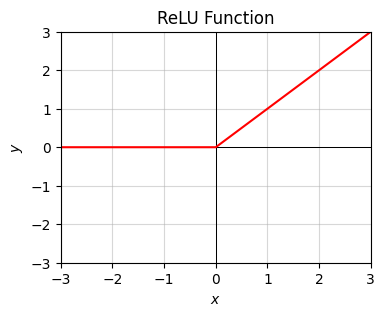
\includegraphics{notebooks/basic-math_files/figure-pdf/cell-27-output-1.png}

}

\end{figure}

Last, I'll mention here the \textbf{absolute value} function
\(y = |x|\), defined by the piecewise function

\[
y = \begin{cases}
x & \text{if } x \ge 0 \\
-x & \text{if } x < 0.
\end{cases}
\]

The absolute value just ignores negative signs and makes everything
positive. The function looks like the usual line \(y=x\) when positive,
but like the negative-sloped line \(y=-x\) when negative. At \(x=0\) the
two lines meet, creating a distinctive v-shape. To get the absolute
value function in python, use \texttt{abs} or \texttt{np.abs}.

\begin{Shaded}
\begin{Highlighting}[]
\NormalTok{x }\OperatorTok{=}\NormalTok{ np.arange(}\OperatorTok{{-}}\DecValTok{5}\NormalTok{, }\DecValTok{5}\NormalTok{, }\FloatTok{0.1}\NormalTok{)}
\NormalTok{f }\OperatorTok{=} \KeywordTok{lambda}\NormalTok{ x: }\BuiltInTok{abs}\NormalTok{(x)}
\NormalTok{plot\_function(x, f, xlim}\OperatorTok{=}\NormalTok{(}\OperatorTok{{-}}\DecValTok{5}\NormalTok{, }\DecValTok{5}\NormalTok{), ylim}\OperatorTok{=}\NormalTok{(}\DecValTok{0}\NormalTok{, }\DecValTok{5}\NormalTok{), ticks\_every}\OperatorTok{=}\NormalTok{[}\DecValTok{1}\NormalTok{, }\DecValTok{1}\NormalTok{], }
\NormalTok{              title}\OperatorTok{=}\StringTok{\textquotesingle{}Absolute Value Function: $y=|x|$\textquotesingle{}}\NormalTok{)}
\end{Highlighting}
\end{Shaded}

\begin{figure}[H]

{\centering 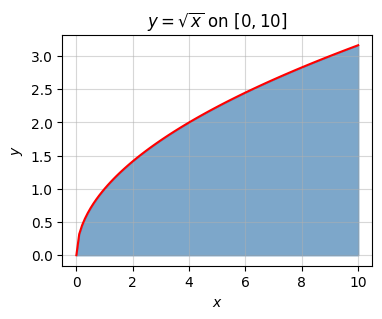
\includegraphics{notebooks/basic-math_files/figure-pdf/cell-28-output-1.png}

}

\end{figure}

\hypertarget{composite-functions}{%
\subsection{Composite Functions}\label{composite-functions}}

We can also have any arbitrary hybrid of the above functions. We can
apply exponentials to affine functions, logs to sine functions, sines to
exponential functions. In essence, this kind of layered composition of
functions is what a neural network is as we'll see later on.

Math folks often write an abstract compositional function as a function
applied to another function, like \(y=f(g(x))\) or \(y=(f \circ g)(x)\).
These can be chained arbitrarily many times, not just two. Neural
networks do just that, often hundreds or thousands of times.

Consider, for example, the function composition done by applying the
following functions in sequence:

\begin{itemize}
\tightlist
\item
  an affine function \(f(x) = wx+b\)
\item
  followed by a linear function \(g(x) = -x\)
\item
  followed by an exponential function \(h(x)=e^x\)
\item
  followed by a rational function \(r(x)=\frac{1}{x}\)
\end{itemize}

to get the full function \[y = r(h(g(x))) = \frac{1}{1 + e^{-(wx+b)}}.\]

Here's a plot of what this function looks like for the ``standard form''
where \(w=1, b=0\). Notice that \(0 \leq y \leq 1\). The values of \(x\)
get ``squashed'' to values between 0 and 1 after the function is
applied.

\begin{Shaded}
\begin{Highlighting}[]
\NormalTok{x }\OperatorTok{=}\NormalTok{ np.arange(}\OperatorTok{{-}}\DecValTok{10}\NormalTok{, }\DecValTok{10}\NormalTok{, }\FloatTok{0.1}\NormalTok{)}
\NormalTok{f }\OperatorTok{=} \KeywordTok{lambda}\NormalTok{ x:  }\DecValTok{1} \OperatorTok{/}\NormalTok{ (}\DecValTok{1} \OperatorTok{+}\NormalTok{ np.exp(}\OperatorTok{{-}}\NormalTok{x))}
\NormalTok{plot\_function(x, f, xlim}\OperatorTok{=}\NormalTok{(}\OperatorTok{{-}}\DecValTok{6}\NormalTok{, }\DecValTok{6}\NormalTok{), ylim}\OperatorTok{=}\NormalTok{(}\OperatorTok{{-}}\FloatTok{0.2}\NormalTok{, }\FloatTok{1.2}\NormalTok{), ticks\_every}\OperatorTok{=}\NormalTok{[}\DecValTok{2}\NormalTok{, }\FloatTok{0.2}\NormalTok{], }
\NormalTok{              title}\OperatorTok{=}\StringTok{\textquotesingle{}Sigmoid Function\textquotesingle{}}\NormalTok{)}
\end{Highlighting}
\end{Shaded}

\begin{figure}[H]

{\centering 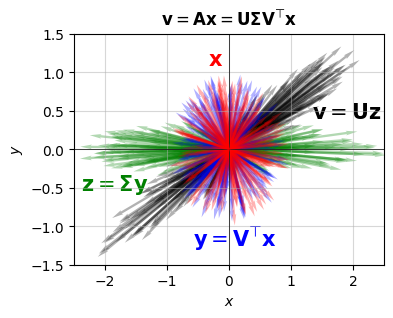
\includegraphics{notebooks/basic-math_files/figure-pdf/cell-29-output-1.png}

}

\end{figure}

This function is called the \textbf{sigmoid} function. The sigmoid is
very important in machine learning since it in essence creates
probabilities. We'll see it a lot more. The standard form sigmoid
function, usually written \(\sigma(x)\), is given by

\[\sigma(x) = \frac{1}{1 + e^{-x}}.\]

Arbitrary affine transformations of the standard form would then be
written as \(\sigma(wx+b)\).

A similar looking function shows up sometimes as well called the
\textbf{hyperbolic tangent} or \textbf{tanh} function, which has the
(standard) form

\[\tanh(x) = \frac{e^x - e^{-x}}{e^x + e^{-x}}.\]

The tanh function looks pretty much the same as the sigmoid except it's
rescaled vertically so that \(-1 \leq y \leq 1\).

Here's a plot of the tanh function. Notice how similar it looks to the
sigmoid with the exception of the scale of the y-axis.

\begin{Shaded}
\begin{Highlighting}[]
\NormalTok{x }\OperatorTok{=}\NormalTok{ np.arange(}\OperatorTok{{-}}\DecValTok{10}\NormalTok{, }\DecValTok{10}\NormalTok{, }\FloatTok{0.1}\NormalTok{)}
\NormalTok{f }\OperatorTok{=} \KeywordTok{lambda}\NormalTok{ x: (np.exp(x) }\OperatorTok{{-}}\NormalTok{ np.exp(}\OperatorTok{{-}}\NormalTok{x)) }\OperatorTok{/}\NormalTok{ (np.exp(x) }\OperatorTok{+}\NormalTok{ np.exp(}\OperatorTok{{-}}\NormalTok{x))}
\NormalTok{plot\_function(x, f, xlim}\OperatorTok{=}\NormalTok{(}\OperatorTok{{-}}\DecValTok{5}\NormalTok{, }\DecValTok{5}\NormalTok{), ylim}\OperatorTok{=}\NormalTok{(}\OperatorTok{{-}}\DecValTok{2}\NormalTok{, }\DecValTok{2}\NormalTok{), ticks\_every}\OperatorTok{=}\NormalTok{[}\DecValTok{1}\NormalTok{, }\FloatTok{0.5}\NormalTok{], }
\NormalTok{              title}\OperatorTok{=}\StringTok{\textquotesingle{}Tanh Function\textquotesingle{}}\NormalTok{)}
\end{Highlighting}
\end{Shaded}

\begin{figure}[H]

{\centering 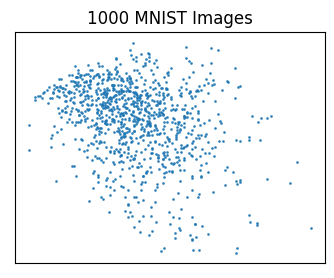
\includegraphics{notebooks/basic-math_files/figure-pdf/cell-30-output-1.png}

}

\end{figure}

\hypertarget{function-transformations}{%
\subsection{Function Transformations}\label{function-transformations}}

Suppose we have some arbitrary function \(f(x)\) and we apply a series
of compositions to get a new function
\[g(x)=a \cdot f(b \cdot (x + c)) + d.\] We can regard each parameter
\(a,b,c,d\) as doing some kind of geometric transformation to the graph
of the original function \(f(x)\). Namely,

\begin{itemize}
\tightlist
\item
  \(a\) re-scales the function vertically (if \(a\) is negative it also
  flips \(f(x)\) upside down)
\item
  \(b\) re-scales the function horizontally (if \(b\) is negative it
  also flips \(f(x)\) left to right)
\item
  \(c\) shifts the function horizontally (left if \(c\) is positive,
  right if \(c\) is negative)
\item
  \(d\) shifts the function vertically (up if \(d\) is positive, down if
  \(d\) is negative)
\end{itemize}

Here's an example of how these work. Consider the function \(f(x)=x^2\).
We're going to apply each of these transformations one by one to show
what they do to the graph of \(f(x)\).

First, let's look at the transformation
\(g(x) = \frac{1}{2} f(x) = \frac{1}{2} x^2\). Here \(a=\frac{1}{2}\)
and the rest are zero. I'll plot it along side the original graph (the
blue curve). Notice the graph gets flattened vertically by a factor of
two (the orange curve).

\begin{Shaded}
\begin{Highlighting}[]
\NormalTok{x }\OperatorTok{=}\NormalTok{ np.arange(}\OperatorTok{{-}}\DecValTok{10}\NormalTok{, }\DecValTok{10}\NormalTok{, }\FloatTok{0.1}\NormalTok{)}
\NormalTok{f }\OperatorTok{=} \KeywordTok{lambda}\NormalTok{ x: x }\OperatorTok{**} \DecValTok{2}
\end{Highlighting}
\end{Shaded}

\begin{Shaded}
\begin{Highlighting}[]
\NormalTok{a }\OperatorTok{=} \DecValTok{1} \OperatorTok{/} \DecValTok{2}
\NormalTok{g }\OperatorTok{=} \KeywordTok{lambda}\NormalTok{ x: a }\OperatorTok{*}\NormalTok{ x }\OperatorTok{**} \DecValTok{2}
\NormalTok{plot\_function(x, [f, g], xlim}\OperatorTok{=}\NormalTok{(}\OperatorTok{{-}}\DecValTok{3}\NormalTok{, }\DecValTok{3}\NormalTok{), ylim}\OperatorTok{=}\NormalTok{(}\OperatorTok{{-}}\DecValTok{2}\NormalTok{, }\DecValTok{10}\NormalTok{), ticks\_every}\OperatorTok{=}\NormalTok{[}\DecValTok{1}\NormalTok{, }\DecValTok{2}\NormalTok{], }
\NormalTok{              title}\OperatorTok{=}\SpecialStringTok{f\textquotesingle{}$a=}\SpecialCharTok{\{}\NormalTok{a}\SpecialCharTok{\}}\SpecialStringTok{$\textquotesingle{}}\NormalTok{)}
\end{Highlighting}
\end{Shaded}

\begin{figure}[H]

{\centering 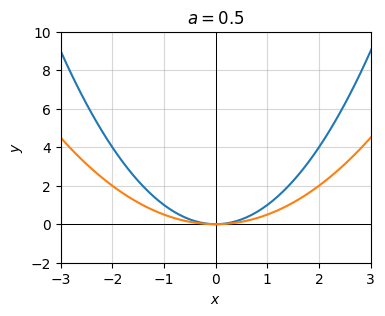
\includegraphics{notebooks/basic-math_files/figure-pdf/cell-32-output-1.png}

}

\end{figure}

Now consider at the transformation

\[g(x) = f\big(\frac{1}{2} x\big) = \bigg(\frac{1}{2} x \bigg)^2.\]

Here \(b=\frac{1}{2}\) and the rest are zero. Notice the graph again
gets flattened but in a slightly different way.

\begin{Shaded}
\begin{Highlighting}[]
\NormalTok{b }\OperatorTok{=} \DecValTok{1} \OperatorTok{/} \DecValTok{2}
\NormalTok{g }\OperatorTok{=} \KeywordTok{lambda}\NormalTok{ x: (b }\OperatorTok{*}\NormalTok{ x) }\OperatorTok{**} \DecValTok{2}
\NormalTok{plot\_function(x, [f, g], xlim}\OperatorTok{=}\NormalTok{(}\OperatorTok{{-}}\DecValTok{3}\NormalTok{, }\DecValTok{3}\NormalTok{), ylim}\OperatorTok{=}\NormalTok{(}\OperatorTok{{-}}\DecValTok{2}\NormalTok{, }\DecValTok{10}\NormalTok{), ticks\_every}\OperatorTok{=}\NormalTok{[}\DecValTok{1}\NormalTok{, }\DecValTok{2}\NormalTok{], }
\NormalTok{              title}\OperatorTok{=}\SpecialStringTok{f\textquotesingle{}$b=}\SpecialCharTok{\{}\NormalTok{b}\SpecialCharTok{\}}\SpecialStringTok{$\textquotesingle{}}\NormalTok{)}
\end{Highlighting}
\end{Shaded}

\begin{figure}[H]

{\centering 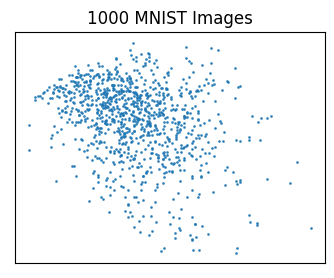
\includegraphics{notebooks/basic-math_files/figure-pdf/cell-33-output-1.png}

}

\end{figure}

Next, consider the transformation \(g(x) = f(x-1) = (x-1)^2.\) Here
\(c=1\) and the rest are zero. Notice the graph's shape doesn't change.
It just gets shifted \emph{right} by \(c=1\) since \(c\) is negative.

\begin{Shaded}
\begin{Highlighting}[]
\NormalTok{c }\OperatorTok{=} \OperatorTok{{-}}\DecValTok{1}
\NormalTok{g }\OperatorTok{=} \KeywordTok{lambda}\NormalTok{ x: (x }\OperatorTok{+}\NormalTok{ c) }\OperatorTok{**} \DecValTok{2}
\NormalTok{plot\_function(x, [f, g], xlim}\OperatorTok{=}\NormalTok{(}\OperatorTok{{-}}\DecValTok{3}\NormalTok{, }\DecValTok{3}\NormalTok{), ylim}\OperatorTok{=}\NormalTok{(}\OperatorTok{{-}}\DecValTok{7}\NormalTok{, }\DecValTok{7}\NormalTok{), ticks\_every}\OperatorTok{=}\NormalTok{[}\DecValTok{1}\NormalTok{, }\DecValTok{2}\NormalTok{], }
\NormalTok{              title}\OperatorTok{=}\SpecialStringTok{f\textquotesingle{}$c=}\SpecialCharTok{\{}\NormalTok{c}\SpecialCharTok{\}}\SpecialStringTok{$\textquotesingle{}}\NormalTok{)}
\end{Highlighting}
\end{Shaded}

\begin{figure}[H]

{\centering 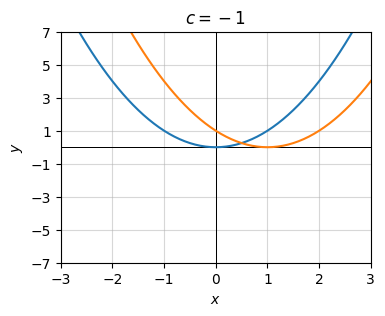
\includegraphics{notebooks/basic-math_files/figure-pdf/cell-34-output-1.png}

}

\end{figure}

Finally, let's look at the transformation \(g(x) = f(x) + 2 = x^2 + 2\).
Here \(d=2\) and the rest are zero. Notice again the graph's shape
doesn't change. It just gets shifted \emph{up} by \(d=2\) units.

\begin{Shaded}
\begin{Highlighting}[]
\NormalTok{d }\OperatorTok{=} \DecValTok{2}
\NormalTok{g }\OperatorTok{=} \KeywordTok{lambda}\NormalTok{ x: x }\OperatorTok{**} \DecValTok{2} \OperatorTok{+}\NormalTok{ d}
\NormalTok{plot\_function(x, [f, g], xlim}\OperatorTok{=}\NormalTok{(}\OperatorTok{{-}}\DecValTok{3}\NormalTok{, }\DecValTok{3}\NormalTok{), ylim}\OperatorTok{=}\NormalTok{(}\OperatorTok{{-}}\DecValTok{1}\NormalTok{, }\DecValTok{8}\NormalTok{), ticks\_every}\OperatorTok{=}\NormalTok{[}\DecValTok{1}\NormalTok{, }\DecValTok{2}\NormalTok{], }
\NormalTok{              title}\OperatorTok{=}\SpecialStringTok{f\textquotesingle{}$d=}\SpecialCharTok{\{}\NormalTok{d}\SpecialCharTok{\}}\SpecialStringTok{$\textquotesingle{}}\NormalTok{)}
\end{Highlighting}
\end{Shaded}

\begin{figure}[H]

{\centering 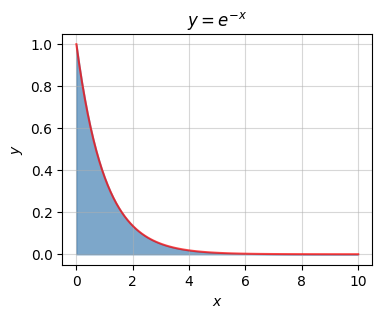
\includegraphics{notebooks/basic-math_files/figure-pdf/cell-35-output-1.png}

}

\end{figure}

Let's now put them all together to see what happens. We should see
rescaling in both directions and shifts in both directions. It's hard to
see in the plot, but it's all there if you zoom in. The vertex of the
parabola is at the point \(x=c=1, y=d=2\). And the stretching factors
due to \(a=b=1/2\) are both acting to flatten the parabola.

\begin{Shaded}
\begin{Highlighting}[]
\NormalTok{g }\OperatorTok{=} \KeywordTok{lambda}\NormalTok{ x: a }\OperatorTok{*}\NormalTok{ (b }\OperatorTok{*}\NormalTok{ (x }\OperatorTok{+}\NormalTok{ c)) }\OperatorTok{**} \DecValTok{2} \OperatorTok{+}\NormalTok{ d}
\NormalTok{plot\_function(x, [f, g], xlim}\OperatorTok{=}\NormalTok{(}\OperatorTok{{-}}\DecValTok{8}\NormalTok{, }\DecValTok{8}\NormalTok{), ylim}\OperatorTok{=}\NormalTok{(}\OperatorTok{{-}}\DecValTok{2}\NormalTok{, }\DecValTok{10}\NormalTok{), ticks\_every}\OperatorTok{=}\NormalTok{[}\DecValTok{2}\NormalTok{, }\DecValTok{2}\NormalTok{], }
\NormalTok{              title}\OperatorTok{=}\SpecialStringTok{f\textquotesingle{}$a=}\SpecialCharTok{\{}\NormalTok{a}\SpecialCharTok{\}}\SpecialStringTok{, b=}\SpecialCharTok{\{}\NormalTok{b}\SpecialCharTok{\}}\SpecialStringTok{, c=}\SpecialCharTok{\{}\NormalTok{c}\SpecialCharTok{\}}\SpecialStringTok{, d=}\SpecialCharTok{\{}\NormalTok{d}\SpecialCharTok{\}}\SpecialStringTok{$\textquotesingle{}}\NormalTok{)}
\end{Highlighting}
\end{Shaded}

\begin{figure}[H]

{\centering 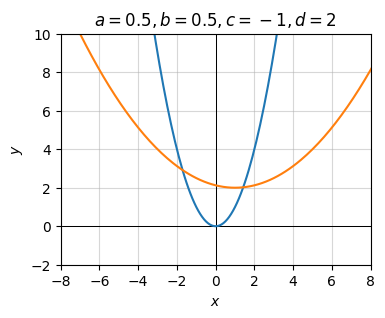
\includegraphics{notebooks/basic-math_files/figure-pdf/cell-36-output-1.png}

}

\end{figure}

\hypertarget{multivariate-functions}{%
\section{Multivariate Functions}\label{multivariate-functions}}

What we've covered thus far only deals with univariate functions,
functions where \(y=f(x)\), but \(x\) and \(y\) are just single numbers,
i.e.~scalars. In machine learning we're almost always dealing with
multivariate functions with \emph{lots} of variables, sometimes billions
of them. It turns out that most of what I've covered so far extends
straight forwardly to multivariate functions with some small caveats,
which I'll cover below.

Simply put, a multivariate function is a function of multiple variables.
Instead of a single variable \(x\), we might have several variables,
e.g.~\(x_0, x_1, x_2, x_3, x_4, x_5\),

\[y = f(x_0, x_1, x_2, x_3, x_4, x_5).\]

If you think about mathematical functions analogously to python
functions it shouldn't be surprising functions can have multiple
arguments. They usually do, in fact.

Here's an example of a function that takes two arguments \(x\) and \(y\)
and produces a single output \(z\), more often written as a
\emph{bivariate function} \(z=f(x,y)\). The example I'll look at is
\(z = x^2 + y^2\). I'll evaluate the function at three points:

\begin{itemize}
\tightlist
\item
  \(x=0\), \(y=0\),
\item
  \(x=1\), \(y=-1\),
\item
  \(x=0\), \(y=1\).
\end{itemize}

The main thing to notice is the function does exactly what you think it
does. If you plug in 2 values, you get out 1 value.

\begin{Shaded}
\begin{Highlighting}[]
\NormalTok{f }\OperatorTok{=} \KeywordTok{lambda}\NormalTok{ x, y: x }\OperatorTok{**} \DecValTok{2} \OperatorTok{+}\NormalTok{ y }\OperatorTok{**} \DecValTok{2}
\BuiltInTok{print}\NormalTok{(}\SpecialStringTok{f\textquotesingle{}z = f}\SpecialCharTok{\{}\NormalTok{(}\DecValTok{0}\NormalTok{, }\DecValTok{0}\NormalTok{)}\SpecialCharTok{\}}\SpecialStringTok{ = }\SpecialCharTok{\{}\NormalTok{f(}\DecValTok{0}\NormalTok{, }\DecValTok{0}\NormalTok{)}\SpecialCharTok{\}}\SpecialStringTok{\textquotesingle{}}\NormalTok{)}
\BuiltInTok{print}\NormalTok{(}\SpecialStringTok{f\textquotesingle{}z = f}\SpecialCharTok{\{}\NormalTok{(}\DecValTok{1}\NormalTok{, }\OperatorTok{{-}}\DecValTok{1}\NormalTok{)}\SpecialCharTok{\}}\SpecialStringTok{ = }\SpecialCharTok{\{}\NormalTok{f(}\DecValTok{1}\NormalTok{, }\OperatorTok{{-}}\DecValTok{1}\NormalTok{)}\SpecialCharTok{\}}\SpecialStringTok{\textquotesingle{}}\NormalTok{)}
\BuiltInTok{print}\NormalTok{(}\SpecialStringTok{f\textquotesingle{}z = f}\SpecialCharTok{\{}\NormalTok{(}\DecValTok{0}\NormalTok{, }\DecValTok{1}\NormalTok{)}\SpecialCharTok{\}}\SpecialStringTok{ = }\SpecialCharTok{\{}\NormalTok{f(}\DecValTok{0}\NormalTok{, }\DecValTok{1}\NormalTok{)}\SpecialCharTok{\}}\SpecialStringTok{\textquotesingle{}}\NormalTok{)}
\end{Highlighting}
\end{Shaded}

\begin{verbatim}
z = f(0, 0) = 0
z = f(1, -1) = 2
z = f(0, 1) = 1
\end{verbatim}

We can also have functions that map multiple inputs to multiple outputs.
Suppose we have a function that takes in 2 values \(x_0, x_1\) and
outputs 2 values \(y_0, y_1\). We'd write this as
\((y_0, y_1) = f(x_0, x_1)\).

Consider the following example,

\[(y_0, y_1) = f(x_0, x_1) = (x_0+x_1, x_0-x_1).\]

This is really just two functions, both functions of \(x_0\) and
\(x_1\). We can completely equivalently write this function as

\[y_0 = f_1(x_0, x_1) = x_0+x_1,\] \[y_1 = f_2(x_0, x_1) = x_0-x_1.\]

Here's this function defined and evaluated at the point \(x_0=1\),
\(x_1=1\).

\begin{Shaded}
\begin{Highlighting}[]
\NormalTok{f }\OperatorTok{=} \KeywordTok{lambda}\NormalTok{ x0, x1: (x0 }\OperatorTok{+}\NormalTok{ x1, x0 }\OperatorTok{{-}}\NormalTok{ x1)}
\BuiltInTok{print}\NormalTok{(}\SpecialStringTok{f\textquotesingle{}(y0, y1) = }\SpecialCharTok{\{}\NormalTok{f(}\DecValTok{1}\NormalTok{, }\DecValTok{1}\NormalTok{)}\SpecialCharTok{\}}\SpecialStringTok{\textquotesingle{}}\NormalTok{)}
\end{Highlighting}
\end{Shaded}

\begin{verbatim}
(y0, y1) = (2, 0)
\end{verbatim}

For now I'll just focus on the case of multiple inputs, single output
like the first example. These are usually called \textbf{scalar-valued
functions}. We can also have \textbf{vector-valued functions}, which are
functions whose \emph{outputs} can have multiple values as well. I'll
focus on scalar-valued functions here.

A scalar-valued function of \(n\) variables
\(x_0, x_1, \cdots, x_{n-1}\) has the form

\[y = f(x_0, x_1, \cdots, x_{n-1}).\]

Note \(n\) can be as large as we want it to be. When working with deep
neural networks (which are just multivariate functions of a certain
form) \(n\) can be huge. For example, if the input is a
\(256 \times 256\) image, the input might be \(256^2=65536\) pixels. For
a 10 second audio clip that's sampled at 44 kHz, the input might be
\(10*44k=440k\) amplitudes. Large numbers indeed.

Calculating the output of multivariate functions is just as
straight-forward as for univariate functions pretty much. Unfortunately,
visualizing them is much harder. The human eye can't see 65536
dimensions, only 3 dimensions. This in some sense means we need to give
up on the ability to ``graph'' a function and instead find other ways to
visualize it.

One thing that sometimes help to visualize high dimension functions is
to pretend they're functions of two variables, like \(z=f(x,y)\). In
this special case we can visualize the inputs as an xy-plane, and the
output as a third axis sticking out perpendicular to the xy-plane from
the origin. Each \(x,y\) pair will map to one unique \(z\) value. Done
this way, we won't get a graph of a \emph{curve} as before, but a
\emph{surface}.

Here's an example of what this might look like for the simple function
\(z=x^2+y^2\). I'll plot the function on the domain
\(-10 \leq x \leq 10\) and \(-10 \leq y \leq 10\) using the helper
function \texttt{plot\_3d}. It takes in two lists of values \texttt{x}
and \texttt{y}. I'll use \texttt{np.linspace} to sample 100 points from
-10 to 10 for each. Then I'll define a lambda function that maps
\texttt{x} and \texttt{y} to the output \texttt{z}. Passing these three
arguments into the helper function gives us our 3D plot.

\begin{Shaded}
\begin{Highlighting}[]
\NormalTok{x }\OperatorTok{=}\NormalTok{ np.linspace(}\OperatorTok{{-}}\DecValTok{10}\NormalTok{, }\DecValTok{10}\NormalTok{, }\DecValTok{100}\NormalTok{)}
\NormalTok{y }\OperatorTok{=}\NormalTok{ np.linspace(}\OperatorTok{{-}}\DecValTok{10}\NormalTok{, }\DecValTok{10}\NormalTok{, }\DecValTok{100}\NormalTok{)}
\NormalTok{f }\OperatorTok{=} \KeywordTok{lambda}\NormalTok{ x, y: x}\OperatorTok{**}\DecValTok{2} \OperatorTok{+}\NormalTok{ y}\OperatorTok{**}\DecValTok{2}
\end{Highlighting}
\end{Shaded}

\begin{Shaded}
\begin{Highlighting}[]
\NormalTok{plot\_function\_3d(x, y, f, title}\OperatorTok{=}\StringTok{\textquotesingle{}3D Plot: $z=x\^{}2+y\^{}2$\textquotesingle{}}\NormalTok{, }
\NormalTok{                 ticks\_every}\OperatorTok{=}\NormalTok{[}\DecValTok{5}\NormalTok{, }\DecValTok{5}\NormalTok{, }\DecValTok{50}\NormalTok{], labelpad}\OperatorTok{=}\DecValTok{5}\NormalTok{, dist}\OperatorTok{=}\DecValTok{12}\NormalTok{)}
\end{Highlighting}
\end{Shaded}

\begin{figure}[H]

{\centering 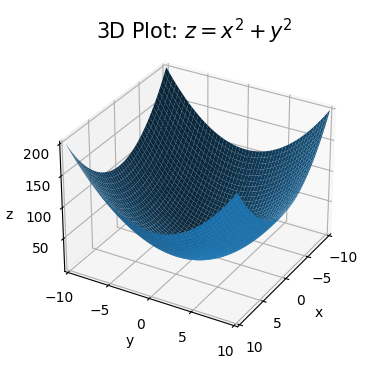
\includegraphics{notebooks/basic-math_files/figure-pdf/cell-40-output-1.png}

}

\end{figure}

Notice how the plot looks like an upward facing bowl. Imagine a bowl
lying on a table. The table is the xy-plane. The bowl is the surface
\(z=x^2+y^2\) we're plotting. While the plot shows the general idea
what's going on, 3D plots can often be difficult to look at. They're
often slanted at funny angles and hide important details.

Here's another way we can visualize the same function: Rather than
create a third axis for \(z\), we can plot it directly on the xy-plane
as a 2D plot. Since we're dealing with a surface, not a curve, we have
to do this for lots of different \(z\) values, which will give a
\emph{family} of curves. For example, we might plot all of the following
curves corresponding to different values of \(z\) in the xy-plane,

\begin{align}
25 &= x^2 + y^2, \\
50 &= x^2 + y^2, \\
75 &= x^2 + y^2, \\
100 &= x^2 + y^2, \\
125 &= x^2 + y^2, \\
150 &= x^2 + y^2.
\end{align}

Doing this will give a family of curves on one 2D plot, with each curve
representing some value of \(z\). In our example, these curves are all
circles of radius \(z^2\). Each curve is called a \textbf{level curve}
or \textbf{level set}.

These kinds of plots are called \textbf{contour plots}. A contour map
can be thought of as looking at the surface from the top down, where
each level set corresponds to slicing the function \(z=f(x,y)\)
horizontally for different values of \(z\). This trick is often used in
topographical maps to visualize 3D terrain on a 2D sheet of paper. Here
is a contour plot for \(z=x^2+y^2\) using the above level curves.

\begin{Shaded}
\begin{Highlighting}[]
\NormalTok{plot\_countour(x, y, f, title}\OperatorTok{=}\StringTok{\textquotesingle{}Countour Plot: $z=x\^{}2+y\^{}2$\textquotesingle{}}\NormalTok{)}
\end{Highlighting}
\end{Shaded}

\begin{figure}[H]

{\centering 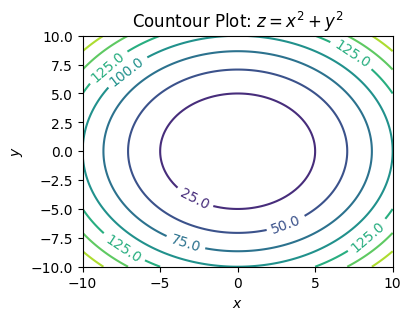
\includegraphics{notebooks/basic-math_files/figure-pdf/cell-41-output-1.png}

}

\end{figure}

Notice how we get a bunch of concentric rings in the contour plot, each
labeled by some value (their \(z\) values). These rings correspond to
the circles I was talking about. You can visually imagine this plot as
looking down from the top of the bowl. In the middle you see the bottom.
The rings get closer together the further out you go, which indicates
that the bowl is sloping steeper the further out we get.

We'll see more examples of multivariate functions in the coming lessons.

\hypertarget{systems-of-equations}{%
\section{Systems of Equations}\label{systems-of-equations}}

In machine learning we'll find ourselves frequently interested not just
with single equations, but multiple equations each with many variables.
One thing we might seek to do is solve these coupled systems, which
means finding a solution that satisfies every equation simultaneously.
Consider the following example,

\begin{alignat*}{3}
   x & {}+{} &  y & {}={} & 2  \\
   2x & {}-{} &  3y & {}={} & 7.
\end{alignat*}

This system consists of two equations, \(x + y = 2\), and
\(2x - 3y = 7\). Each equation contains two unknown variables, \(x\) and
\(y\). We need to find a solution for both \(x\) and \(y\) that
satisfies both of these equations.

Usually the easiest and most general way to solve simple coupled systems
like this is the \textbf{method of substitution}. The idea is to solve
one equation for one variable in terms of the other, then plug that
solution into the second equation to solve for the other variable. Once
the second variable is solved for, we can go back and solve for the
first variable explicitly. Let's start by solving the first equation for
\(x\) in terms of \(y\). This is pretty easy,

\[x = 2 - y.\]

Now we can take this solution for \(x\) and plug it into the second
equation to solve for \(y\),

\begin{align*}
2x - 3y &= 7 \\
2(2 - y) - 3y &= 7 \\
4 - 5y &= 7 \\
5y &= -3 \\
y &= -\frac{3}{5}.
\end{align*}

With \(y\) in hand, we can now solve for \(x\),
\(x = 2 - y = 2 + \frac{3}{5} = \frac{13}{5}\). Thus, the pair
\(x=\frac{13}{5}\), \(y=-\frac{3}{5}\) is the solution that solves both
of these coupled equations simultaneously.

Here's sympy's solution to the same system. It should of course agree
with what I just got, which it does.

\begin{Shaded}
\begin{Highlighting}[]
\NormalTok{x, y }\OperatorTok{=}\NormalTok{ sp.symbols(}\StringTok{\textquotesingle{}x y\textquotesingle{}}\NormalTok{)}
\NormalTok{eq1 }\OperatorTok{=}\NormalTok{ sp.Eq(x }\OperatorTok{+}\NormalTok{ y, }\DecValTok{2}\NormalTok{)}
\NormalTok{eq2 }\OperatorTok{=}\NormalTok{ sp.Eq(}\DecValTok{2} \OperatorTok{*}\NormalTok{ x }\OperatorTok{{-}} \DecValTok{3} \OperatorTok{*}\NormalTok{ y, }\DecValTok{7}\NormalTok{)}
\NormalTok{sol }\OperatorTok{=}\NormalTok{ sp.solve((eq1, eq2), (x, y))}
\BuiltInTok{print}\NormalTok{(}\SpecialStringTok{f\textquotesingle{}x = }\SpecialCharTok{\{}\NormalTok{sol[x]}\SpecialCharTok{\}}\SpecialStringTok{\textquotesingle{}}\NormalTok{)}
\BuiltInTok{print}\NormalTok{(}\SpecialStringTok{f\textquotesingle{}y = }\SpecialCharTok{\{}\NormalTok{sol[y]}\SpecialCharTok{\}}\SpecialStringTok{\textquotesingle{}}\NormalTok{)}
\end{Highlighting}
\end{Shaded}

\begin{verbatim}
x = 13/5
y = -3/5
\end{verbatim}

Notice that both of the equations in this example are \emph{linear},
since each term only contains terms proportional to \(x\) and \(y\).
There are no terms like \(x^2\) or \(\sin y\) or whatever. Linear
systems of equations are special because they can always be solved as
long as there are enough variables. I'll spend a lot more time on these
when I get to linear algebra.

We can also imagine one or more equations being \emph{nonlinear}.
Provided we can solve each equation one-by-one, we can apply the method
of substitution to solve these too. Here's an example. Consider the
nonlinear system

\begin{align*}
e^{x + y} &= 10  \\
xy &= 1.
\end{align*}

Let's solve the second equation first since it's easier. Solving for
\(y\) gives \(y = \frac{1}{x}\). Now plug this into the first equation
and solve for \(x\),

\begin{align*}
e^{x + y} &= 10  \\
e^{x + 1/x} &= 10  \\
\log \big(e^{x + 1/x}\big) &= \log 10 \\
x + \frac{1}{x} &= \log 10 \\
x^2 - \log 10 \cdot x + 1 &= 0 \\
x &= \frac{1}{2} \bigg(\log 10 \pm \sqrt{(\log 10)^2 - 4}\bigg) \\
x &\approx 0.581, \ 1.722.
\end{align*}

Note here I had to use the \textbf{quadratic formula}, which I'll assume
you've forgotten. If you have a quadratic equation of the form
\(ax^2 + bx + c = 0\), then it will (usually) have exactly two solutions
given by the formula

\[x = \frac{1}{2a} \bigg(-b \pm \sqrt{b^2 - 4ac}\bigg).\]

This means we have two different possible solutions for \(x\), which
thus means we'll also have two possible solutions to \(y\) since
\(y=\frac{1}{x}\). Thus, this system has \emph{two} possible solutions,

\[\text{Solution 1: }x \approx 0.581, \ y \approx 1.722,\]
\[\text{Solution 2: }x \approx 1.722, \ y \approx 0.581.\]

It's interesting how symmetric these two solutions are. They're
basically the same with \(x\) and \(y\) swapped. This is because the
system has symmetry. You can swap \(x\) and \(y\) in the system above
and not change the equation, which means the solutions must be the same
up to permutation of \(x\) and \(y\)!

Here's sympy's attempt to solve this system.

\begin{Shaded}
\begin{Highlighting}[]
\NormalTok{x, y }\OperatorTok{=}\NormalTok{ sp.symbols(}\StringTok{\textquotesingle{}x y\textquotesingle{}}\NormalTok{)}
\NormalTok{eq1 }\OperatorTok{=}\NormalTok{ sp.Eq(sp.exp(x }\OperatorTok{+}\NormalTok{ y), }\DecValTok{10}\NormalTok{)}
\NormalTok{eq2 }\OperatorTok{=}\NormalTok{ sp.Eq(x }\OperatorTok{*}\NormalTok{ y, }\DecValTok{1}\NormalTok{)}
\NormalTok{sol }\OperatorTok{=}\NormalTok{ sp.solve((eq1, eq2), (x, y))}
\BuiltInTok{print}\NormalTok{(}\SpecialStringTok{f\textquotesingle{}x1 = }\SpecialCharTok{\{}\NormalTok{sol[}\DecValTok{0}\NormalTok{][}\DecValTok{0}\NormalTok{]}\SpecialCharTok{.}\BuiltInTok{round}\NormalTok{(}\DecValTok{5}\NormalTok{)}\SpecialCharTok{\}}\SpecialStringTok{ }\CharTok{\textbackslash{}t}\SpecialStringTok{ y1 = }\SpecialCharTok{\{}\NormalTok{sol[}\DecValTok{0}\NormalTok{][}\DecValTok{1}\NormalTok{]}\SpecialCharTok{.}\BuiltInTok{round}\NormalTok{(}\DecValTok{5}\NormalTok{)}\SpecialCharTok{\}}\SpecialStringTok{\textquotesingle{}}\NormalTok{)}
\BuiltInTok{print}\NormalTok{(}\SpecialStringTok{f\textquotesingle{}x2 = }\SpecialCharTok{\{}\NormalTok{sol[}\DecValTok{1}\NormalTok{][}\DecValTok{0}\NormalTok{]}\SpecialCharTok{.}\BuiltInTok{round}\NormalTok{(}\DecValTok{5}\NormalTok{)}\SpecialCharTok{\}}\SpecialStringTok{ }\CharTok{\textbackslash{}t}\SpecialStringTok{ y2 = }\SpecialCharTok{\{}\NormalTok{sol[}\DecValTok{1}\NormalTok{][}\DecValTok{1}\NormalTok{]}\SpecialCharTok{.}\BuiltInTok{round}\NormalTok{(}\DecValTok{5}\NormalTok{)}\SpecialCharTok{\}}\SpecialStringTok{\textquotesingle{}}\NormalTok{)}
\end{Highlighting}
\end{Shaded}

\begin{verbatim}
x1 = 0.58079     y1 = 1.72180
x2 = 1.72180     y2 = 0.58079
\end{verbatim}

In general, it's not even possible to solve a system of nonlinear
equations except using numerical methods. The example I gave was rigged
so I could solve it by hand. General purpose \textbf{root-finding}
algorithms exist that can solve arbitrary systems of equations like this
numerically, no matter how nonlinear they are.

To solve a nonlinear system like this numerically, you can use the scipy
function \texttt{scipy.optimize.fsolve}. Scipy is an extension of numpy
that includes a lot of algorithms for working with non-linear functions.
To use \texttt{fsolve}, you have to define the system as a function
mapping a list of variables to a list of equations. You also have to
specify a starting point \texttt{x0} for the root finder. This tells it
where to start looking for the root. Since nonlinear equations have
multiple solutions, picking a different \texttt{x0} can and will often
give you a different root. I won't dwell on all this since we don't
really need to deal with root finding much in machine learning.

\begin{Shaded}
\begin{Highlighting}[]
\ImportTok{from}\NormalTok{ scipy.optimize }\ImportTok{import}\NormalTok{ fsolve}

\NormalTok{system }\OperatorTok{=} \KeywordTok{lambda}\NormalTok{ xy: [np.exp(xy[}\DecValTok{0}\NormalTok{] }\OperatorTok{+}\NormalTok{ xy[}\DecValTok{1}\NormalTok{]) }\OperatorTok{{-}} \DecValTok{10}\NormalTok{, xy[}\DecValTok{0}\NormalTok{] }\OperatorTok{*}\NormalTok{ xy[}\DecValTok{1}\NormalTok{] }\OperatorTok{{-}} \DecValTok{1}\NormalTok{]}
\NormalTok{solution }\OperatorTok{=}\NormalTok{ fsolve(system, x0}\OperatorTok{=}\NormalTok{(}\DecValTok{1}\NormalTok{, }\DecValTok{1}\NormalTok{))}
\BuiltInTok{print}\NormalTok{(}\SpecialStringTok{f\textquotesingle{}solution = }\SpecialCharTok{\{}\NormalTok{solution}\SpecialCharTok{\}}\SpecialStringTok{\textquotesingle{}}\NormalTok{)}
\end{Highlighting}
\end{Shaded}

\begin{verbatim}
solution = [0.5807888 1.7217963]
\end{verbatim}

\hypertarget{sums-and-products}{%
\section{Sums and Products}\label{sums-and-products}}

\hypertarget{sums}{%
\subsection{Sums}\label{sums}}

We typically find ourselves performing operations on large numbers of
numbers at a time. By far the most common operation is adding up a bunch
of numbers, or \textbf{summation}. Suppose we have some
\textbf{sequence} of \(n\) numbers \(x_0,x_1,x_2,\cdots,x_{n-1}\). They
could be anything, related by a function, or not. If we wanted to sum
them together to get a new number \(x\) we could write

\[x = x_0 + x_1 + x_2 + \cdots + x_{n-1}.\]

But it's kind of cumbersome to always write like this. For this reason
in math there's a more compact notation to write sums called
\textbf{summation notation}. We introduce the symbol \(\sum\) for
``sum'', and write \[x = \sum_{i=0}^{n-1} x_i.\]

Read this as ``the sum of all \(x_i\) for \(i=0,1,\cdots,n-1\) is
\(x\)''. The index \(i\) being summed over is called a \textbf{dummy
index}. It can be whatever we want since it never appears on the
left-hand side. It gets summed over and then disappears. The lower and
upper values \(i=0\) and \(i=n-1\) are the \textbf{limits} of the
summation. The limits need not always be \(i=0\) and \(i=n-1\). We can
choose them to be whatever we like as a matter of convenience.

Frequently summation notation is paired with some kind of
\textbf{generating function} \(f(i) = x_i\) that generates the sequence.
For example, suppose our sequence is generated by the function
\(f(i) = i\), and we want to sum from \(i=1\) to \(i=n\). We'd have

\[x = \sum_{i=1}^n x_i = \sum_{i=1}^n i = 1 + 2 + \cdots + n = \frac{1}{2} n(n+1).\]

The right-hand term \(\frac{1}{2} n(n-1)\) is not obvious, and only
applies to this particular sum. I just wrote it down since it's
sometimes useful to remember. This is a special kind of sum called an
\textbf{arithmetic series}. Here's a ``proof'' of this relationship
using sympy.

\begin{Shaded}
\begin{Highlighting}[]
\NormalTok{i, n }\OperatorTok{=}\NormalTok{ sp.symbols(}\StringTok{\textquotesingle{}i n\textquotesingle{}}\NormalTok{)}
\NormalTok{summation }\OperatorTok{=}\NormalTok{ sp.Sum(i, (i, }\DecValTok{1}\NormalTok{, n)).doit()}
\BuiltInTok{print}\NormalTok{(}\SpecialStringTok{f\textquotesingle{}sum i for i=1,...,n = }\SpecialCharTok{\{}\NormalTok{summation}\SpecialCharTok{\}}\SpecialStringTok{\textquotesingle{}}\NormalTok{)}
\end{Highlighting}
\end{Shaded}

\begin{verbatim}
sum i for i=1,...,n = n**2/2 + n/2
\end{verbatim}

In the general case when we don't have nice rules like this we'd have to
loop over the entire sum and do the sum incrementally.

In python, the equivalent of summation notation is the \texttt{sum}
function, where we pass in the sequence we want to sum as a list. Here's
the arithmetic sum up to \(n=10\), which should be
\(\frac{1}{2} 10 \cdot (10+1) = 55\).

\begin{Shaded}
\begin{Highlighting}[]
\BuiltInTok{sum}\NormalTok{([}\DecValTok{1}\NormalTok{, }\DecValTok{2}\NormalTok{, }\DecValTok{3}\NormalTok{, }\DecValTok{4}\NormalTok{, }\DecValTok{5}\NormalTok{, }\DecValTok{6}\NormalTok{, }\DecValTok{7}\NormalTok{, }\DecValTok{8}\NormalTok{, }\DecValTok{9}\NormalTok{, }\DecValTok{10}\NormalTok{])}
\end{Highlighting}
\end{Shaded}

\begin{verbatim}
55
\end{verbatim}

Another useful sum to be aware of is the \textbf{geometric series}. A
geometric series is a sum over a sequence whose generating function is
\(f(i) = r^i\) for some real number \(r \neq 1\). Its rule is

\[x = \sum_{i=0}^{n-1} r^i = r^0 + r^1 + \cdots + r^{n-1} = \frac{1-r^n}{1-r}.\]

For example, if \(n=10\) and \(r=\frac{1}{2}\), we have

\[x = \sum_{i=0}^{9} \bigg(\frac{1}{2}\bigg)^i = \frac{1-\big(\frac{1}{2}\big)^{10}}{1-\big(\frac{1}{2}\big)} = 2\bigg(1-\frac{1}{2^{10}}\bigg) \approx 1.998.\]

\begin{Shaded}
\begin{Highlighting}[]
\NormalTok{r }\OperatorTok{=} \DecValTok{1} \OperatorTok{/} \DecValTok{2}
\NormalTok{n }\OperatorTok{=} \DecValTok{10}
\BuiltInTok{sum}\NormalTok{([r }\OperatorTok{**}\NormalTok{ i }\ControlFlowTok{for}\NormalTok{ i }\KeywordTok{in} \BuiltInTok{range}\NormalTok{(n)])}
\end{Highlighting}
\end{Shaded}

\begin{verbatim}
1.998046875
\end{verbatim}

Notice how the term \(\big(\frac{1}{2}\big)^{10} \approx 0.00098\) is
really small. We can practically ignore it. In fact, as
\(n \rightarrow \infty\) we can completely ignore it, in which case

\[x = \sum_{i=0}^{\infty} \bigg(\frac{1}{2}\bigg)^i = \frac{1}{1-\big(\frac{1}{2}\big)} = 2.\]

This is an example of the infinite version of the geometric series. If
\(0 \leq r \leq 1\), then

\[x = \sum_{i=0}^{\infty} r^i = r^0 + r^1 + r^2 + \cdots = \frac{1}{1-r}.\]

What happens when \(r=1\)? Clearly the rule breaks down at this point,
since the denominator becomes infinite. But it's easy enough to see what
it is by writing out the sum,

\[x = \sum_{i=0}^{n-1} 1^i = 1^0 + 1^1 + \cdots + 1^{n-1} = \underbrace{1 + 1 + \cdots + 1}_{\text{n times}} = n.\]

In this case, if we send \(n \rightarrow \infty\), then \(x\) clearly
blows up to \(\infty\) too. You can see this by plotting the function
\(y = \frac{1}{1-x}\) and observing it asymptotes at \(x=1\).

\begin{Shaded}
\begin{Highlighting}[]
\NormalTok{x }\OperatorTok{=}\NormalTok{ np.arange(}\DecValTok{0}\NormalTok{, }\DecValTok{1}\NormalTok{, }\FloatTok{0.01}\NormalTok{)}
\NormalTok{f }\OperatorTok{=} \KeywordTok{lambda}\NormalTok{ x: }\DecValTok{1} \OperatorTok{/}\NormalTok{ (}\DecValTok{1} \OperatorTok{{-}}\NormalTok{ x)}
\NormalTok{plot\_function(x, f, xlim}\OperatorTok{=}\NormalTok{(}\DecValTok{0}\NormalTok{, }\DecValTok{1}\NormalTok{), ylim}\OperatorTok{=}\NormalTok{(}\DecValTok{0}\NormalTok{, }\DecValTok{100}\NormalTok{), ticks\_every}\OperatorTok{=}\NormalTok{[}\FloatTok{0.2}\NormalTok{, }\DecValTok{20}\NormalTok{], }
\NormalTok{              title}\OperatorTok{=}\StringTok{\textquotesingle{}$y=1/(1{-}x)$\textquotesingle{}}\NormalTok{)}
\end{Highlighting}
\end{Shaded}

\begin{figure}[H]

{\centering 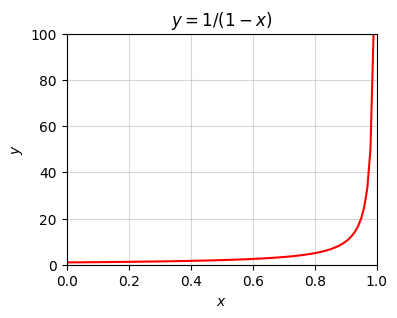
\includegraphics{notebooks/basic-math_files/figure-pdf/cell-48-output-1.png}

}

\end{figure}

We can always factor constants \(c\) out of sums. This follows naturally
from just expanding the sum out,

\[\sum_{i=0}^{n-1} c x_i = cx_0 + cx_1 + \cdots + cx_{n-1} = c(x_0 + x_1 + \cdots + x_{n-1}) = c\sum_{i=0}^{n-1} x_i.\]

Similarly, we can break sums up into pieces (or join sums together) as
long as we're careful to get the index limits right,

\[\sum_{i=0}^{n-1} x_i = \sum_{i=0}^{k} x_i + \sum_{i=k+1}^{n-1} x_i.\]

We can have double sums (sums of sums) as well. If \(x_{i,j}\) is some
2-index variable where \(i=0,\cdots,n-1\) and \(j=0,\cdots,m-1\), we can
sum over both sets of indices to get \(n \cdot m\) total terms,

\[\sum_{i=0}^{n-1} \sum_{j=0}^{m-1} x_{i,j} = \sum_{j=0}^{m-1} \sum_{i=0}^{n-1} x_{i,j} = x_{0,0} + x_{0,1} + \cdots x_{0,m-1} + \cdots + x_{n-1,0} + x_{n-1,1} + \cdots x_{n-1,m-1}.\]

Notice the two sums can swap, or \textbf{commute}, with each other,
\(\sum_i \sum_j = \sum_j \sum_i\). This follows by expanding the terms
out like on the right-hand side and noting the must be equal in both
cases.

\hypertarget{products}{%
\subsection{Products}\label{products}}

The notation I've covered for sums has an analogue for products, called
\textbf{product notation}. Suppose we want to multiply \(n\) numbers
\(x_0,x_1,\cdots,x_{n-1}\) together to get some number \(x\). We could
write

\[x = x_0 \cdot x_1 \cdots x_{n-1},\]

but we have a more compact notation for this as well. Using the symbol
\(\prod\) in analogy to \(\sum\), we can write

\[x = \prod_{i=0}^{n-1} x_i.\]

Read this as ``the product of all \(x_i\) for \(i=0,1,\cdots,n-1\) is
\(x\)''.

Unlike sums, python doesn't have a native function to calculate products
of elements in a sequence, but numpy has one called \texttt{np.prod}.
Here's an example. I'll calculate the product of all integers between
one and ten.

\[x = \prod_{i=1}^{10} i = 1 \cdot 2 \cdot 3 \cdot 4 \cdot 5 \cdot 6 \cdot 7 \cdot 8 \cdot 9 \cdot 10 = 3628800.\]

\begin{Shaded}
\begin{Highlighting}[]
\NormalTok{np.prod([}\DecValTok{1}\NormalTok{, }\DecValTok{2}\NormalTok{, }\DecValTok{3}\NormalTok{, }\DecValTok{4}\NormalTok{, }\DecValTok{5}\NormalTok{, }\DecValTok{6}\NormalTok{, }\DecValTok{7}\NormalTok{, }\DecValTok{8}\NormalTok{, }\DecValTok{9}\NormalTok{, }\DecValTok{10}\NormalTok{])}
\end{Highlighting}
\end{Shaded}

\begin{verbatim}
3628800
\end{verbatim}

Luckily, there aren't any common products to remember. It's just worth
being familiar with the notation, since we'll occasionally use it.

Products don't obey quite the same properties sums do, so you have to be
careful. When in doubt, just write out the product the long way and make
sure what you're doing makes sense. For example, pulling a factor \(c\)
out of a product gives a factor of \(c^n\), not \(c\), since there are
\(c\) total products multiplied together,

\[x = \prod_{i=0}^{n-1} cx_i = cx_0 \cdot cx_1 \cdots cx_{n-1} = c^n(x_0 \cdot x_1 \cdots x_{n-1}) = c^n \prod_{i=0}^{n-1} x_i.\]

It's worth noting (because we'll use this fact), that we can turn
products into sums by taking the log of the product,

\[\log \bigg(\prod_{i=0}^{n-1} x_i \bigg) = \sum_{i=0}^{n-1} \log x_i.\]

This follows from the rule \(\log(x \cdot y) = \log x + \log y\), which
extends to arbitrarily many products too.

\hypertarget{greek-alphabet}{%
\section{Greek Alphabet}\label{greek-alphabet}}

Like many other technical fields, machine learning makes heavy use of
the Greek alphabet to represent variable names in mathematical
equations. While not all Greek characters are used, certain ones are
worth being aware of. Below is a
\href{https://howtosaymathematics.files.wordpress.com/2011/08/greek-alphabet2.pdf}{table}
of the Greek letters. You don't need to memorize all of these letters,
but it's worth referencing this table whenever you encounter a symbol
you don't recognize.

\bookmarksetup{startatroot}

\hypertarget{numerical-computation}{%
\chapter{Numerical Computation}\label{numerical-computation}}

In this lesson I'll discuss the basics of numerical computation. This
includes how numbers are represented on a computer, as well as the
topics of arrays and vectorization, which is the use of efficient array
operations to speed up computations.This may seem too basic to mention,
but it's actually very important. There's a lot of subtlety involved.
Let's get started.

\begin{Shaded}
\begin{Highlighting}[]
\ImportTok{import}\NormalTok{ numpy }\ImportTok{as}\NormalTok{ np}
\ImportTok{from}\NormalTok{ utils.math\_ml }\ImportTok{import} \OperatorTok{*}
\end{Highlighting}
\end{Shaded}

\hypertarget{integers}{%
\section{Integers}\label{integers}}

\hypertarget{basics}{%
\subsection{Basics}\label{basics}}

Recall the \textbf{integers} are whole numbers that can be positive,
negative, or zero. Examples are 5, 100151, 0, -72, etc. The set of all
integers is commonly denoted by the symbol \(\mathbb{Z}\).

In python, integers (ints for short) are builtin objects of type
\texttt{int} that more or less follow the rules that integers in math
follow.

Among other things, the following operations can be performed with
integers:

\begin{itemize}
\tightlist
\item
  Addition: \(2 + 2 = 4\).
\item
  Subtraction: \(2 - 5 = -3\).
\item
  Multiplication: \(3 \cdot 3 = 9\)

  \begin{itemize}
  \tightlist
  \item
    In python this is the \texttt{*} operator,
    e.g.~\texttt{3\ *\ 3\ =\ 9}
  \end{itemize}
\item
  Exponentiation: \(2^3 = 2 \times 2 \times 2 = 8\)

  \begin{itemize}
  \tightlist
  \item
    In python this is the \texttt{**} operator,
    e.g.~\texttt{2\ **\ 3\ =\ 8}.
  \end{itemize}
\item
  Remainder (or Modulo): the remainder of 10 when divided by 3 is 1,
  written \(10 \text{ mod } 3 = 1\)

  \begin{itemize}
  \tightlist
  \item
    In python this is the \texttt{\%} operator,
    e.g.~\texttt{10\ \%\ 3\ =\ 1}.
  \end{itemize}
\end{itemize}

If any of these operations are applied to two integers, the output will
itself always be an integer.

Here are a few examples.

\begin{Shaded}
\begin{Highlighting}[]
\DecValTok{2} \OperatorTok{+} \DecValTok{2}
\end{Highlighting}
\end{Shaded}

\begin{verbatim}
4
\end{verbatim}

\begin{Shaded}
\begin{Highlighting}[]
\DecValTok{2} \OperatorTok{{-}} \DecValTok{5}
\end{Highlighting}
\end{Shaded}

\begin{verbatim}
-3
\end{verbatim}

\begin{Shaded}
\begin{Highlighting}[]
\DecValTok{3} \OperatorTok{*} \DecValTok{3}
\end{Highlighting}
\end{Shaded}

\begin{verbatim}
9
\end{verbatim}

\begin{Shaded}
\begin{Highlighting}[]
\DecValTok{10} \OperatorTok{\%} \DecValTok{3}
\end{Highlighting}
\end{Shaded}

\begin{verbatim}
1
\end{verbatim}

\begin{Shaded}
\begin{Highlighting}[]
\DecValTok{2} \OperatorTok{**} \DecValTok{3}
\end{Highlighting}
\end{Shaded}

\begin{verbatim}
8
\end{verbatim}

What about division? You can't always divide two integers and get
another integer. What you have to do instead is called integer division.
Here you divide the two numbers and then round the answer down to the
nearest whole number. Since \(5 \div 2 = 2.5\), the nearest rounded down
integer is 2.

In math, this ``nearest rounded down integer'' 2 is usually called the
\textbf{floor} of 2.5, and represented with the funny symbol
\(\lfloor 2.5 \rfloor.\) Using this notation we can write the above
integer division as \[\big\lfloor \frac{5}{2} \big\rfloor = 2.\]

In python, integer division is done using the \texttt{//} operator,
e.g.~\texttt{5\ //\ 2\ =\ 2}. I'll usually write \(5 \ // \ 2\) instead
of \(\big\lfloor \frac{5}{2} \big\rfloor\) when it makes sense,
\[5 \ // \ 2 = \big\lfloor \frac{5}{2} \big\rfloor = 2.\]

\begin{Shaded}
\begin{Highlighting}[]
\DecValTok{5} \OperatorTok{//} \DecValTok{2}
\end{Highlighting}
\end{Shaded}

\begin{verbatim}
2
\end{verbatim}

We can also do regular division \texttt{/} with ints, but the output
will \emph{not} be an integer even if the answer should be,
e.g.~\texttt{4\ /\ 2}. Only integer division is guaranteed to return an
integer. I'll get to this shortly.

\begin{Shaded}
\begin{Highlighting}[]
\DecValTok{4} \OperatorTok{/} \DecValTok{2}
\BuiltInTok{type}\NormalTok{(}\DecValTok{4} \OperatorTok{/} \DecValTok{2}\NormalTok{)}
\end{Highlighting}
\end{Shaded}

\begin{verbatim}
2.0
\end{verbatim}

\begin{verbatim}
float
\end{verbatim}

\begin{Shaded}
\begin{Highlighting}[]
\DecValTok{4} \OperatorTok{//} \DecValTok{2}
\BuiltInTok{type}\NormalTok{ (}\DecValTok{4} \OperatorTok{//} \DecValTok{2}\NormalTok{)}
\end{Highlighting}
\end{Shaded}

\begin{verbatim}
2
\end{verbatim}

\begin{verbatim}
int
\end{verbatim}

Division by zero is of course undefined for both division and integer
division. In python it will always raise a \texttt{ZeroDivisionError}
like so.

\begin{Shaded}
\begin{Highlighting}[]
\DecValTok{4} \OperatorTok{/} \DecValTok{0}
\end{Highlighting}
\end{Shaded}

\begin{verbatim}
ZeroDivisionError: division by zero
\end{verbatim}

\begin{Shaded}
\begin{Highlighting}[]
\DecValTok{4} \OperatorTok{//} \DecValTok{0}
\end{Highlighting}
\end{Shaded}

\begin{verbatim}
ZeroDivisionError: integer division or modulo by zero
\end{verbatim}

\hypertarget{representing-integers}{%
\subsection{Representing Integers}\label{representing-integers}}

Just like every other data type, on a computer integers are actually
represented internally as a sequence of bits. A \textbf{bit} is a
``binary digit'', 0 or 1. A sequence of bits is just a sequence of zeros
and ones, e.g.~0011001010 or 1001001.

The number of bits used to represent a piece of data is called its
\textbf{word size}. If we use a word size of \(n\) bits to represent an
integer, then there are \(2^n\) possible integer values we can
represent.

If integers could only be positive or zero, representing them with bits
would be easy. We could just convert them to binary and that's it. To
convert a non-negative integer to binary, we just need to keep dividing
it by 2 and recording its remainder (0 or 1) at each step. The binary
form is then just the sequence of remainders, written right to left.
More generally, the binary sequence of some arbitrary number \(x\) is
the sequence of coefficients \(b_k=0,1\) in the sum

\[x = \sum_{k=-\infty}^\infty b_k 2^k = \cdots + b_2 2^2 + b_1 2^1 + b_0 2^0 + b_{-1} 2^{-1} + b_{-2} 2^{-2} + \cdots.\]

Here's an example. Suppose we wanted to represent the number \(12\) in
binary.

\begin{enumerate}
\def\labelenumi{\arabic{enumi}.}
\tightlist
\item
  \(12 \ // \ 2 = 6\) with a remainder of \(0 = 12 \text{ mod } 2\), so
  the first bit from the right is then \(0\).
\item
  \(6 \ // \ 2 = 3\) with a remainder of \(0 = 6 \text{ mod } 2\), so
  the next bit is \(0\).
\item
  \(3 \ // \ 2 = 1\) with a remainder of \(1 = 3 \text{ mod } 2\), so
  the next bit is \(1\).
\item
  \(1 \ // \ 2 = 0\) with a remainder of \(1 = 1 \text{ mod } 2\), so
  the next bit is \(1\).
\end{enumerate}

So the binary representation of \(12\) is \(1100\), which is the
sequence of coefficients in the sum

\[12 = 1 \cdot 2^{3} + 1 \cdot 2^{2} + 0 \cdot 2^{1} + 0 \cdot 2^{0}.\]

Rather than keep doing these by hand, you can quickly convert a number
to binary in python by using \texttt{bin}. It'll return a string
representing the binary sequence of that number, prepended with the
special prefix \texttt{0b}. To get back to the integer from, use
\texttt{int}, passing in a base of \texttt{2}.

\begin{Shaded}
\begin{Highlighting}[]
\BuiltInTok{bin}\NormalTok{(}\DecValTok{12}\NormalTok{)}
\end{Highlighting}
\end{Shaded}

\begin{verbatim}
'0b1100'
\end{verbatim}

\begin{Shaded}
\begin{Highlighting}[]
\BuiltInTok{int}\NormalTok{(}\StringTok{\textquotesingle{}0b110\textquotesingle{}}\NormalTok{, }\DecValTok{2}\NormalTok{)}
\end{Highlighting}
\end{Shaded}

\begin{verbatim}
6
\end{verbatim}

This representation works fine for non-negative integers, also called
the \textbf{unsigned integers} in computer science. To represent an
unsigned integer with \(n\) bits, just get its binary form and prepend
it with enough zeros on the left until all \(n\) bits are used. For
example, if we used 8-bit unsigned integers then \(n=8\), hence
representing the number \(12\) would look like \(00000110\). Simple,
right?

Unsigned ints work fine if we never have to worry about negative
numbers. But in general we do. These are called the \textbf{signed
integers} in computer science. To represent signed ints, we need to use
one of the bits to represent the sign. What we can do is reserve the
left-most bit for the sign, \(0\) if the integers is positive or zero,
\(1\) if the integer is negative.

For example, if we used 8-bit \emph{signed} integers to represent
\(12\), we'd again write \(00000110\), exactly as before. But this time
it's understood that left-most \(0\) is encoding the fact that \(12\) is
positive. If instead we wanted to represent the number \(-12\) we'd need
to flip that bit to a \(1\), so we'd get \(10000110\).

Let's now do an example of a simple integer system. Consider the system
of 4-bit signed ints. In this simple system, \(n=4\) is the word size,
and an integer \(x\) is represented with the sequence of bits

\[x \equiv sb_1b_2b_3,\]

where \(s\) is the sign bit and \(b_1b_2b_3\) are the remaining 3 bits
allowed to represent the numerical digits. This system can represent
\(2^4=16\) possible values in the range \([-2^3+1,2^3-1] = [-8,7]\),
given in the following table:

\begin{longtable}[]{@{}llll@{}}
\toprule()
Integer & Representation & Integer & Representation \\
\midrule()
\endhead
-0 & 1000 & +0 & 0000 \\
-1 & 1001 & 1 & 0001 \\
-2 & 1010 & 2 & 0010 \\
-3 & 1011 & 3 & 0011 \\
-4 & 1100 & 4 & 0100 \\
-5 & 1101 & 5 & 0101 \\
-6 & 1110 & 6 & 0110 \\
-7 & 1111 & 7 & 0111 \\
\bottomrule()
\end{longtable}

Note the presence of \(-0 \equiv 1110\) in the upper left. This is
because the system as I've defined it leaves open the possibility of two
zeros, \(+0\) and \(-0\), since for zero the sign bit is redundant. A
way to get around this is to encode the negative numbers slightly
differently, by not just setting the sign bit to one, but also inverting
the remaining bits and subtracting one from them. This is called the
\textbf{two's complement representation}. It's how most languages,
including python, actually represent integers. I won't go into this
representation in any depth, except to say that it gets rid of the need
for \(-0\) and replaces it with \(-2^{n-1}\).

Here's what that table looks like for 4-bit integers. It's almost the
same, except there's no \(-0\), instead a \(-8\). Notice the positive
integers look exactly the same. It's only the negative integers that
look different. For them, the right three bits get inverted and added
with a one.

\begin{longtable}[]{@{}llll@{}}
\toprule()
Integer & Two's Complement & Integer & Two's Complement \\
\midrule()
\endhead
-1 & 1111 & 0 & 0000 \\
-2 & 1110 & 1 & 0001 \\
-3 & 1101 & 2 & 0010 \\
-4 & 1100 & 3 & 0011 \\
-5 & 1011 & 4 & 0100 \\
-6 & 1010 & 5 & 0101 \\
-7 & 1001 & 6 & 0110 \\
-8 & 1000 & 7 & 0111 \\
\bottomrule()
\end{longtable}

It's worth visualizing what integers look like on the number line, if
for nothing else than to compare it with what floats look like later on.
Below I'll plot what a 6-bit signed integer system would look like. Such
a system should go from -32 to 31. As you'd expect, we get a bunch of
equally spaced points from -32 to 31.

\begin{Shaded}
\begin{Highlighting}[]
\NormalTok{n }\OperatorTok{=} \DecValTok{6}
\NormalTok{six\_bit\_ints }\OperatorTok{=} \BuiltInTok{range}\NormalTok{(}\OperatorTok{{-}}\DecValTok{2}\OperatorTok{**}\NormalTok{(n}\OperatorTok{{-}}\DecValTok{1}\NormalTok{), }\DecValTok{2}\OperatorTok{**}\NormalTok{(n}\OperatorTok{{-}}\DecValTok{1}\NormalTok{))}
\NormalTok{plot\_number\_dist(six\_bit\_ints, title}\OperatorTok{=}\SpecialStringTok{f\textquotesingle{}Distribution of }\SpecialCharTok{\{}\NormalTok{n}\SpecialCharTok{\}}\SpecialStringTok{{-}bit Signed Ints\textquotesingle{}}\NormalTok{)}
\end{Highlighting}
\end{Shaded}

\begin{figure}[H]

{\centering \includegraphics{notebooks/numerical-computing_files/figure-pdf/cell-16-output-1.png}

}

\end{figure}

In python, integers are represented by default using a much bigger word
size of \(n=64\) bits, called \textbf{long} integers, or \textbf{int64}
for short. This means (using two's complement) we can represent
\(2^{64}=18446744073709551616\) possible integer values in the range
\([-2^{63}, 2^{63}-1]\).

You can see from this that 64-bit integers have a minimum integer
allowed and a maximum integer allowed, which are

\[\text{min\_int}=-2^{63}=-9223372036854775808, \qquad \text{max\_int}=2^{63}-1=9223372036854775807.\]

What I've said is technically only exactly true in older versions of
pythons as well as other programming languages like C. It turns out
newer versions of python have a few added tricks that allow you to
represent essentially arbitrarily large integers. You can see this by
comparing it to numpy's internal int64 representation, which uses the C
version. A numpy int64 outside the valid range will throw an overflow
error.

\begin{Shaded}
\begin{Highlighting}[]
\NormalTok{min\_int }\OperatorTok{=} \OperatorTok{{-}}\DecValTok{2} \OperatorTok{**} \DecValTok{63}
\NormalTok{max\_int }\OperatorTok{=} \DecValTok{2} \OperatorTok{**} \DecValTok{63} \OperatorTok{{-}} \DecValTok{1}
\end{Highlighting}
\end{Shaded}

\begin{Shaded}
\begin{Highlighting}[]
\NormalTok{min\_int }\OperatorTok{{-}} \DecValTok{1}
\NormalTok{np.int64(min\_int }\OperatorTok{{-}} \DecValTok{1}\NormalTok{)}
\end{Highlighting}
\end{Shaded}

\begin{verbatim}
-9223372036854775809
\end{verbatim}

\begin{verbatim}
OverflowError: Python int too large to convert to C long
\end{verbatim}

\begin{Shaded}
\begin{Highlighting}[]
\NormalTok{max\_int }\OperatorTok{+} \DecValTok{1}
\NormalTok{np.int64(max\_int }\OperatorTok{+} \DecValTok{1}\NormalTok{)}
\end{Highlighting}
\end{Shaded}

\begin{verbatim}
9223372036854775808
\end{verbatim}

\begin{verbatim}
OverflowError: Python int too large to convert to C long
\end{verbatim}

\hypertarget{floats}{%
\section{Floats}\label{floats}}

\hypertarget{basics-1}{%
\subsection{Basics}\label{basics-1}}

What if we want to represent decimal numbers or fractions instead of
whole numbers, like \(1.2\) or \(0.99999\), or even irrational numbers
like \(\pi=3.1415926\dots\)? To do this we need a new system of numbers
that I'll call floating point numbers, or \textbf{floats}, for reasons
I'll explain soon. Floats will be a computer's best attempt to represent
the real numbers \(\mathbb{R}\). They'll represent real numbers only
approximately with some specified precision.

In python, floats are builtin objects of type \texttt{float}. Floats
obey pretty much the same operations that integers do with some minor
exceptions:

\begin{itemize}
\tightlist
\item
  Addition: \(1.2 + 4.3 = 5.5\).
\item
  Subtraction: \(1.2 - 4.3 = -3.1\).
\item
  Multiplication: \(1.2 \times 4.3 = 5.16\).
\item
  Exponentiation: \(4.3^2 = 18.49\).
\item
  Remainder (or Modulo): \(4.3 \text{ mod } 1.2 = 0.7\).
\item
  Integer Division: \(4.3 \ // \ 1.2 = 3.0\).
\item
  Division: \(4.3 \div 1.2\).
\end{itemize}

Let's verify the first few of these to see what's going on.

\begin{Shaded}
\begin{Highlighting}[]
\FloatTok{1.2} \OperatorTok{+} \FloatTok{4.3}
\end{Highlighting}
\end{Shaded}

\begin{verbatim}
5.5
\end{verbatim}

\begin{Shaded}
\begin{Highlighting}[]
\FloatTok{1.2} \OperatorTok{{-}} \FloatTok{4.3}
\end{Highlighting}
\end{Shaded}

\begin{verbatim}
-3.0999999999999996
\end{verbatim}

\begin{Shaded}
\begin{Highlighting}[]
\FloatTok{1.2} \OperatorTok{*} \FloatTok{4.3}
\end{Highlighting}
\end{Shaded}

\begin{verbatim}
5.159999999999999
\end{verbatim}

Most of them look right. But what the heck is going on with
\(1.2 - 4.3\) and \(1.2 \times 4.3\)? We're getting some weird trailing
nines that shouldn't be there. This gets to how floats are actually
represented on a computer.

\hypertarget{representing-floats}{%
\subsection{Representing Floats}\label{representing-floats}}

Representing real numbers on a computer is a lot more subtle than
representing integers. Since a computer can only have a finite number of
bits, they can't represent infinitely many digits, e.g.~in irrational
numbers like \(\pi\). Using finite word sizes will necessarily have to
truncate real numbers to some number of decimal places. This truncation
will create an error in the calculation called \textbf{numerical
roundoff}.

So how should we represent a decimal number using \(n\) bits? As an
example, let's imagine we're trying to represent the number
\(x=157.208\). Perhaps the first thing you might think of is to use some
number of those bits to represent the integer part, and some number to
represent the fractional part. Suppose you have \(n=16\) bits available
to represent \(x\). Then maybe you can use 8 bits for the integer part
\(157\), and 8 bits for the fractional part \(0.208\). Converting both
halves to binary, you'd get
\[157 \equiv 10011101, \quad 0.208 \equiv 0011010100111111.\]

Truncating both sequences to 8 bits (from the left), you could thus
adopt a convention that \(157.208 \equiv 10011101 \ 00110101\).

This system is an example of a \textbf{fixed point} representation. This
has to do with the fact that we're always using a fixed number of bits
for the integer part, and a fixed number for the fractional part. The
decimal point isn't allowed to \textbf{float}, or move around to
allocate more bits to the integer or fractional part depending which
needs more precision. The decimal point is \textbf{fixed}.

As I've suggested, the fixed point representation seems to be limited
and not terribly useful. If you need really high precision in the
fractional part, your only option is to use a larger word size. If
you're dealing with really big numbers and don't care much about the
fractional part, you also need a larger word size so you don't run out
of numbers. A solution to this problem is to allow the decimal point to
float. We won't allocate a fixed number of bits to represent the integer
or fractional parts. We'll design it in such a way that larger numbers
give the integer part more bits, and smaller numbers give the fractional
part more bits.

The trick to allowing the decimal point to float is to represent not
just the digits of a number but also its exponent. Think about
scientific notation, where if you have a number like say \(x=1015.23\),
you can write it as \(1.01523 \cdot 10^3\), or \texttt{1.01523e3}. That
\(3\) is the exponent. It says something about how big the number is.
What we can do is convert a number to scientific notation. Then use some
number of bits to represent the exponent \(3\) and some to represent the
remaining part \(1.01523\). This is essentially the whole idea behind
floating point.

In floating point representation, instead of using scientific notation
with powers of ten, it's more typical to use powers of two. When using
powers of two, the decimal part can always be scaled to be between 1 and
2, so they look like \(1.567\) or something like that. Since the \(1.\)
part is always there, we can agree it's always there, and only worry
about representing the fractional part \(0.567\). We'll call this term
the \textbf{mantissa}. Denoting the sign bit as \(s\), the exponent as
\(e\), and the mantissa as \(m\), we can thus right any decimal number
\(x\) in a modified scientific notation of the form
\[x = (-1)^s \cdot (1+m) \cdot 2^{e}.\] Once we've converted \(x\) to
this form, all we need to do is to figure out how to represent \(s\),
\(m\), and \(e\) using some number of bits of \(n\), called the floating
point \textbf{precision}. Assume the \(n\) bits of precision allocate
\(1\) bit for the sign, \(n_e\) bits for the exponent, and \(n_m\) bits
for the mantissa, so \(n=1+n_e+n_m\).

Here are the steps to convert a number \(x\) into its \(n\)-bit floating
point representation.

\begin{itemize}
\tightlist
\item
  Given some number \(x\), get its modified scientific notation form
  \(x = (-1)^s \cdot (1+m) \cdot 2^e\).

  \begin{itemize}
  \tightlist
  \item
    Determine the sign of \(x\). If negative, set the sign bit to
    \(s=1\), else default to \(s=0\). Set \(x = |x|\).
  \item
    Keep performing the operation \(x = x \ // \ 2\) until
    \(1 \leq x \leq 2\). Keep track of the number of times you're
    dividing, which is the \textbf{exponent} \(e\).
  \item
    The remaining part will be some \(1 \leq x \leq 2\). Write it in the
    form \(x = 1 + m\), where \(m\) is the mantissa.
  \end{itemize}
\item
  Convert the scientific notation form into a sequence of \(n\) bits,
  truncating where necessary.

  \begin{itemize}
  \tightlist
  \item
    For reasons I'll describe in a second, it's good to add a
    \textbf{bias} term \(b\) to the exponent \(e\) before converting the
    exponent to binary. Let \(e'=e+b\) be this modified exponent.
  \item
    Convert each of \(e'\) and \(m\) into binary sequences, truncated to
    sizes \(n_e\), and \(n_m\) respectively.
  \item
    Concatenate these binary sequences together to get a sequence of
    \(n=1+n_e+n_m\) total bits. By convention, assume the order of bit
    concatenation is the sign bit, then exponent bits, then the mantissa
    bits.
  \end{itemize}
\end{itemize}

There are of course other ways you could do it, for example by storing
the sequences in a different order. I'm just stating one common way it's
done.

Since all of this must seem like Greek, here's a quick example. Let's
consider the number \(x=15.25\). We'll represent it using \(n=8\) bits
of precision, where \(n_e=4\) is the number of exponent bits, \(n_m=3\)
is the number of precision bits, and \(b=10\) is the bias.

\begin{itemize}
\tightlist
\item
  Convert \(x=15.25\) to its modified scientific notation.

  \begin{itemize}
  \tightlist
  \item
    Since \(x \geq 0\) the sign is positive, so \(s=0\).
  \item
    Keep integer dividing \(x\) by \(2\) until it's less than \(2\). It
    takes \(e=3\) divisions before \(x<2\).
  \item
    We now have \(x = 1.90625 \cdot 2^3\). The mantissa is then
    \(m = (1.90625-1) = 0.90625\).
  \item
    In modified scientific notation form we now have
    \(x=(-1)^0 \cdot (1 + 0.90625) \cdot 2^3\).
  \end{itemize}
\item
  Convert everything to binary.

  \begin{itemize}
  \tightlist
  \item
    Adding the bias to the exponent gives \(e'=3+10=13\).
  \item
    Converting each piece to binary we get \(e' = 13 \equiv 1101\),
    \(m = 0.90625 \equiv 11101\).
  \item
    Since \(m\) requires more than \(n_m=3\) bits to represent, truncate
    off the two right bits to get \(m \equiv 111\).

    \begin{itemize}
    \tightlist
    \item
      This truncation will cause numerical roundoff, since \(0.90625\)
      truncates to \(0.875\). That's an error of \(0.03125\) that gets
      permanently lost.
    \end{itemize}
  \item
    The final representation is thus \(x \equiv 0 \ 1101 \ 111\).
  \end{itemize}
\end{itemize}

Below I show the example I just calculated. I print out both the
scientific notation form and its binary representation.

\begin{Shaded}
\begin{Highlighting}[]
\NormalTok{represent\_as\_float(}\FloatTok{15.25}\NormalTok{, n}\OperatorTok{=}\DecValTok{8}\NormalTok{, n\_exp}\OperatorTok{=}\DecValTok{4}\NormalTok{, n\_man}\OperatorTok{=}\DecValTok{3}\NormalTok{, bias}\OperatorTok{=}\DecValTok{10}\NormalTok{)}
\end{Highlighting}
\end{Shaded}

\begin{verbatim}
scientific notation: (-1)^0 * (1 + 0.90625) * 2^3
8-bit floating point representation: 0 1101 111
\end{verbatim}

So what's going on with the bias term \(b\)? Why do we need it? The
easiest answer to give is that without it, we can't have negative
exponents without having to use another sign bit for them. Consider a
number like \(x=0.5\). In modified scientific notation this would look
like \(x=(-1)^0 \cdot (1+0) \cdot 2^{-1} = 2^{-1}\), meaning its
exponent would be \(e=-1\). Rather than have to keep yet another sign
bit for the exponent, it's easier to just add a bias term \(b\) that
ensures the exponent \(e'=e+b\) is always non-negative. The higher the
bias, the more precision we can show in the range \(-1 < x < 1\). The
trade-off is that we lose precision for large values of \(x\).

On top of floats defined the way I mentioned, we also have some special
numbers that get defined in a floating point system. These are
\(\pm 0\), \(\pm \infty\), and \(\text{NaN}\) or ``not a number''. Each
of these numbers is allocated its own special sequence of bits,
depending on the precision.

\begin{itemize}
\tightlist
\item
  \(+0\) and \(-0\): These numbers are typically represented using a
  biased exponent \(e'=0\) (all zero bits) and a mantissa \(m=0\) (all
  zero bits). The sign bit is used to distinguish between \(+0\) and
  \(-0\). In our example, these would be \(+0 \equiv 0 \ 0000 \ 000\)
  and \(-0 \equiv 1 \ 0000 \ 000\).
\item
  \(+\infty\) and \(-\infty\): These numbers are typically represented
  using the max allowed exponent (all one bits) and a mantissa \(m=0\)
  (all zero bits). The sign bit is used to distinguish between
  \(+\infty\) and \(-\infty\). In our example, these would be
  \(+\infty \equiv 0 \ 1111 \ 000\) and
  \(-\infty \equiv 1 \ 1111 \ 000\).
\item
  \(\text{NaN}\): This value is typically represented using the max
  allowed exponent (all one bits) and a non-zero \(m \neq 0\). The sign
  bit is usually not used for \(\text{NaN}\) values. Note this means we
  can have many different sequences that all represent \(\text{NaN}\).
  In our example, any number of the form
  \(\text{NaN} \equiv \text{x} \ 1111 \ \text{xxx}\) would work.
\end{itemize}

So I can illustrate some points about how floating point numbers behave,
I'm going to generate \emph{all possible} \(8\)-bit floats (excluding
the special numbers) and plot them on a number line, similar to what I
did above with the \(8\)-bit signed integers. I'll generate the floats
using the using the helper function \texttt{gen\_all\_floats}, passing
in the number of mantissa bits \texttt{n\_man=3}, the number of exponent
bits \texttt{n\_exp=4}, and a bias of \texttt{bias=10}.

First, I'll use these numbers to print out some interesting statistics
of this 8-bit floating point system.

\begin{Shaded}
\begin{Highlighting}[]
\NormalTok{eight\_bit\_floats }\OperatorTok{=}\NormalTok{ gen\_all\_floats(n}\OperatorTok{=}\DecValTok{8}\NormalTok{, n\_man}\OperatorTok{=}\DecValTok{3}\NormalTok{, n\_exp}\OperatorTok{=}\DecValTok{4}\NormalTok{, bias}\OperatorTok{=}\DecValTok{10}\NormalTok{)}
\BuiltInTok{print}\NormalTok{(}\SpecialStringTok{f\textquotesingle{}Total number of 8{-}bit floats: }\SpecialCharTok{\{}\BuiltInTok{len}\NormalTok{(eight\_bit\_floats)}\SpecialCharTok{\}}\SpecialStringTok{\textquotesingle{}}\NormalTok{)}
\BuiltInTok{print}\NormalTok{(}\SpecialStringTok{f\textquotesingle{}Most negative float: }\SpecialCharTok{\{}\BuiltInTok{min}\NormalTok{(eight\_bit\_floats)}\SpecialCharTok{\}}\SpecialStringTok{\textquotesingle{}}\NormalTok{)}
\BuiltInTok{print}\NormalTok{(}\SpecialStringTok{f\textquotesingle{}Most positive float: }\SpecialCharTok{\{}\BuiltInTok{max}\NormalTok{(eight\_bit\_floats)}\SpecialCharTok{\}}\SpecialStringTok{\textquotesingle{}}\NormalTok{)}
\BuiltInTok{print}\NormalTok{(}\SpecialStringTok{f\textquotesingle{}Smallest nonzero float: }\SpecialCharTok{\{}\BuiltInTok{min}\NormalTok{([x }\ControlFlowTok{for}\NormalTok{ x }\KeywordTok{in}\NormalTok{ eight\_bit\_floats }\ControlFlowTok{if}\NormalTok{ x }\OperatorTok{\textgreater{}} \DecValTok{0}\NormalTok{])}\SpecialCharTok{\}}\SpecialStringTok{\textquotesingle{}}\NormalTok{)}
\BuiltInTok{print}\NormalTok{(}\SpecialStringTok{f\textquotesingle{}Machine Epsilon: }\SpecialCharTok{\{}\BuiltInTok{min}\NormalTok{([x }\ControlFlowTok{for}\NormalTok{ x }\KeywordTok{in}\NormalTok{ eight\_bit\_floats }\ControlFlowTok{if}\NormalTok{ x }\OperatorTok{\textgreater{}} \DecValTok{1}\NormalTok{]) }\OperatorTok{{-}} \DecValTok{1}\SpecialCharTok{\}}\SpecialStringTok{\textquotesingle{}}\NormalTok{)}
\end{Highlighting}
\end{Shaded}

\begin{verbatim}
Total number of 8-bit floats: 120
Most negative float: -56.0
Most positive float: 56.0
Smallest nonzero float: 0.001953125
Machine Epsilon: 0.25
\end{verbatim}

We can see that this 8-bit system only contains 120 unique floats. We
could practically list them all out. Just like with the integers, we see
there's a most negative float, \(-56.0\), and a most positive float,
\(56.0\). The smallest float, i.e.~the one closest to \(0\), is
\(0.001953125\). Notice how much more precision the smallest float has
than the largest ones do. The largest ones are basically whole numbers,
while the smallest one has nine digits of precision. Evidently, floating
point representations give much higher precision to numbers close to
zero than to numbers far away from zero.

What happens if you try to input a float larger than the max, in this
case \(56.0\)? Typically it will \textbf{overflow}. This will result in
either the system raising an error, or the number getting set to
\(+\infty\), in a sense getting ``rounded up''. Similarly, for numbers
more negative than the min, in this case \(-56.0\), either an overflow
error will be raised, or the number will get ``rounded down'' to
\(-\infty\).

You have to be careful in overflow situations like this, especially when
you don't know for sure which of these your particular system will do.
It's amusing to note that python will raise an overflow error, but numpy
will round to \(\pm \infty\). Two different conventions to worry about.
Just as amusing, when dealing with signed integers, it's numpy that will
raise an error if you overflow, while python won't care. One of those
things\ldots{}

What happens when you try to input a float smaller than the smallest
value, in this case \(0.001953125\)? In this case, the number is said to
\textbf{undeflow}. Usually underflow won't raise an error. The number
will pretty much always just get set to \(+0\) (or \(-0\)). This is
again something you have to worry about, especially if you're dealing
with small numbers in denominators, where they can lead to division by
zero errors which \emph{do} get raised.

Overflow and underflow errors are some of the most common numerical bugs
that occur in deep learning, and usually result from not handling floats
correctly to begin with.

I also printed out a special value called the \textbf{machine epsilon}.
The machine epsilon, denoted \(\varepsilon_m\), is defined as the
smallest value in a floating point system that's larger than \(1\). In
some sense, \(\varepsilon_m\) is a proxy for how finely you can
represent numbers in a given \(n\)-bit floating point system. The
smaller \(\varepsilon_m\) the more precisely you can represent numbers,
i.e.~the more decimal places of precision you get access to. In our
case, we get \(\varepsilon_m=0.25\). This means numbers in 8-bit
floating point tend to be \(0.25\) apart from each other on average,
which means we can represent numbers in this system only with a measly
2-3 digits of precision.

With these numbers in hand let's now plot their distribution on the
number line. Compare with the plot of the signed integers I did above.

\begin{Shaded}
\begin{Highlighting}[]
\NormalTok{plot\_number\_dist(eight\_bit\_floats, title}\OperatorTok{=}\StringTok{\textquotesingle{}Distribution of 8{-}bit Floats\textquotesingle{}}\NormalTok{)}
\end{Highlighting}
\end{Shaded}

\begin{figure}[H]

{\centering \includegraphics{notebooks/numerical-computing_files/figure-pdf/cell-25-output-1.png}

}

\end{figure}

Notice how different this plot is from the ones for the signed integers.
With the integers, the points were equally spaced. Now points close to
\(0\) are getting represented much closer together than points far from
\(0\). There are \(74\) of the \(120\) total points showing up just in
the range \([-1,1]\). That's over half!. Meanwhile, only \(22\) points
total show up in the combined ranges of \([-60,-10]\) and \([10,60]\).
Very strange.

Feel free to play around with different floating point systems by using
different choices for \texttt{n}, \texttt{n\_man}, \texttt{n\_exp}, and
\texttt{bias}. Be careful, however, not to make \texttt{n\_exp} too
large or you may crash the kernel\ldots{}

\hypertarget{double-precision}{%
\subsection{Double Precision}\label{double-precision}}

So how does python represent floats? Python by default uses what's
called \textbf{double precision} to represent floats, also called
\textbf{float64}. This means \(n=64\) total bits of precision are used,
with \(n_e=11\), \(n_m=52\), and bias \(b=1023=2^{10}-1\). Double
precision allows for a \emph{much} larger range of numbers than 8-bit
precision does:

\begin{itemize}
\tightlist
\item
  The max value allowed is
  \(2^{2^{n_e}-b} = 2^{1025} \approx 10^{308}\).
\item
  The min value allowed is
  \(-2^{2^{n_e}-b} = -2^{1025} \approx -10^{308}\).
\item
  Numbers \emph{outside} the range of about \([-10^{308}, 10^{308}]\)
  will \emph{overflow}.
\item
  The smallest values allowed are (plus or minus)
  \(2^{-b+1} = 2^{-1022} \approx 10^{-308}\).

  \begin{itemize}
  \tightlist
  \item
    Using subordinal numbers, the smallest values are (plus or minus)
    \(2^{-b-n_m+1} = 2^{-1074} \approx 10^{-324}\).
  \end{itemize}
\item
  Numbers \emph{inside} the range of about \([-10^{-308}, 10^{-308}]\)
  will \emph{underflow}.

  \begin{itemize}
  \tightlist
  \item
    Using subordinal numbers, this range is around
    \([-10^{-324}, 10^{-324}]\).
  \end{itemize}
\item
  The machine epsilon is \(\varepsilon_m = 2^{-53} \approx 10^{-16}\).
\item
  Numbers requiring more than about 15-16 digits of precision will get
  truncated, resulting in numerical roundoff.
\item
  The special numbers \(\pm \infty\), \(\pm 0\), and \(\text{NaN}\) are
  represented similarly as before, except using 64 bits.
\end{itemize}

To illustrate the point regarding numerical roundoff, here's what
happens if we try to use double precision floating point to define the
constant \(\pi\) to its first
\href{https://www.wolframalpha.com/input?i=pi+to+100+digits}{100
digits}? Notice it just gets truncated to its first 15 digits. Double
precision is unable to keep track of the other 85 digits. They just get
lost to numerical roundoff.

\begin{Shaded}
\begin{Highlighting}[]
\NormalTok{pi }\OperatorTok{=} \FloatTok{3.141592653589793238462643383279502884197169399375105820974944592307816406286208998628034825342117068}
\NormalTok{pi}
\end{Highlighting}
\end{Shaded}

\begin{verbatim}
3.141592653589793
\end{verbatim}

Another thing to worry about is adding small numbers to medium to large
sized numbers, e.g.~\(10 + 10^{-16}\), which will just get rounded down
to \(10.0\).

\begin{Shaded}
\begin{Highlighting}[]
\FloatTok{10.0} \OperatorTok{+} \FloatTok{1e{-}16}
\end{Highlighting}
\end{Shaded}

\begin{verbatim}
10.0
\end{verbatim}

Numerical roundoff is often an issue when subtracting two floats. Here's
what happens when we try to subtract two numbers that should be equal,
\(x=0.1+0.2\) and \(y=0.3\). Instead of \(y-x=0\), we get
\(y-x \approx -5.55 \cdot 10^{-17}\). The problem comes from the
calculation \(x=0.1+0.2\), which caused a slight loss of precision in
\(x\).

\begin{Shaded}
\begin{Highlighting}[]
\NormalTok{x }\OperatorTok{=} \FloatTok{0.1} \OperatorTok{+} \FloatTok{0.2}
\NormalTok{y }\OperatorTok{=} \FloatTok{0.3}
\NormalTok{y }\OperatorTok{{-}}\NormalTok{ x}
\end{Highlighting}
\end{Shaded}

\begin{verbatim}
-5.551115123125783e-17
\end{verbatim}

A major implication of these calculations is that you should
\emph{never} test floating points for exact equality because numerical
roundoff can mess it up. If you'd tried to test something like
\texttt{(y\ -\ x)\ ==\ 0.0}, you'd have gotten the wrong answer.
Instead, you want to test that \texttt{y\ -\ x} is less than some small
number \texttt{tol}, called a \emph{tolerance},
i.e.~\texttt{abs(y\ -\ x)\ \textless{}\ tol}.

\begin{Shaded}
\begin{Highlighting}[]
\NormalTok{y }\OperatorTok{{-}}\NormalTok{ x }\OperatorTok{==} \FloatTok{0.0}
\end{Highlighting}
\end{Shaded}

\begin{verbatim}
False
\end{verbatim}

\begin{Shaded}
\begin{Highlighting}[]
\NormalTok{tol }\OperatorTok{=} \FloatTok{1e{-}5}
\BuiltInTok{abs}\NormalTok{(y }\OperatorTok{{-}}\NormalTok{ x) }\OperatorTok{\textless{}}\NormalTok{ tol}
\end{Highlighting}
\end{Shaded}

\begin{verbatim}
True
\end{verbatim}

Numerical roundoff explains why we got the weird results above when
subtracting \(1.2 - 4.3\). The imperfect precision in the two numbers
resulted in a numerical roundoff error, leading in the trailing \(9\)s
that should've rounded up to \(-3.1\) exactly. In general, subtracting
floats is one of the most dangerous operations to do, as it tends to
lead to the highest loss of precision in calculations. The closer two
numbers are to being equal the worse this loss of precision tends to
get.

I mentioned that double precision has a smallest number of
\(2^{-1022} \approx 10^{-308}\), but caveated that by saying that, by
using a trick called \textbf{subordinal numbers}, we can get the
smallest number down to about \(10^{-324}\). What did I mean by this? It
turns out that the bits where the biased exponent \(e'=0\) (i.e.~all
exponent bits are zero) go mostly unused in the standard version of
double precision. By using this zero exponent and allowing the mantissa
\(m\) to take on all its possible values, we can get about \(2^{52}\)
more values (since the mantissa has 52 bits). This lets us get all the
way down to \(2^{-1022} \cdot 2^{-52} = 2^{-1074} \approx 10^{-324}\).

Python (and numpy) by default implements double precision with
subordinal numbers, as we can see.

\begin{Shaded}
\begin{Highlighting}[]
\DecValTok{2} \OperatorTok{**}\NormalTok{ (}\OperatorTok{{-}}\DecValTok{1074}\NormalTok{)}
\end{Highlighting}
\end{Shaded}

\begin{verbatim}
5e-324
\end{verbatim}

\begin{Shaded}
\begin{Highlighting}[]
\DecValTok{2} \OperatorTok{**}\NormalTok{ (}\OperatorTok{{-}}\DecValTok{1075}\NormalTok{)}
\end{Highlighting}
\end{Shaded}

\begin{verbatim}
0.0
\end{verbatim}

The special numbers \(\pm \infty\), \(\pm 0\), and \(\text{NaN}\) are
also defined in double precision. In python (and numpy) they're given by
the following commands,

\begin{itemize}
\tightlist
\item
  \(\infty\): \texttt{float(\textquotesingle{}inf\textquotesingle{})} or
  \texttt{np.inf},
\item
  \(-\infty\): \texttt{float(\textquotesingle{}-inf\textquotesingle{})}
  or \texttt{-np.inf},
\item
  \(\pm 0\): \texttt{0},
\item
  \(\text{NaN}\):
  \texttt{float(\textquotesingle{}nan\textquotesingle{})} or
  \texttt{np.nan}.
\end{itemize}

\begin{Shaded}
\begin{Highlighting}[]
\BuiltInTok{float}\NormalTok{(}\StringTok{\textquotesingle{}inf\textquotesingle{}}\NormalTok{)}
\NormalTok{np.inf}
\end{Highlighting}
\end{Shaded}

\begin{verbatim}
inf
\end{verbatim}

\begin{verbatim}
inf
\end{verbatim}

\begin{Shaded}
\begin{Highlighting}[]
\BuiltInTok{float}\NormalTok{(}\StringTok{\textquotesingle{}{-}inf\textquotesingle{}}\NormalTok{)}
\OperatorTok{{-}}\NormalTok{np.inf}
\end{Highlighting}
\end{Shaded}

\begin{verbatim}
-inf
\end{verbatim}

\begin{verbatim}
-inf
\end{verbatim}

\begin{Shaded}
\begin{Highlighting}[]
\DecValTok{0}
\OperatorTok{{-}}\DecValTok{0}
\end{Highlighting}
\end{Shaded}

\begin{verbatim}
0
\end{verbatim}

\begin{verbatim}
0
\end{verbatim}

\begin{Shaded}
\begin{Highlighting}[]
\BuiltInTok{float}\NormalTok{(}\StringTok{\textquotesingle{}nan\textquotesingle{}}\NormalTok{)}
\NormalTok{np.nan}
\end{Highlighting}
\end{Shaded}

\begin{verbatim}
nan
\end{verbatim}

\begin{verbatim}
nan
\end{verbatim}

You may be curious what exactly \(\text{NaN}\) (``not a number'') is and
where it might show up. Basically, NaNs are used wherever values are
undefined. Anytime an operation doesn't return a sensible value it risks
getting converted to NaN. One example is the operation
\(\infty - \infty = \infty + (-\infty)\), which mathematically doesn't
make sense. No, it's not zero\ldots{}

\begin{Shaded}
\begin{Highlighting}[]
\BuiltInTok{float}\NormalTok{(}\StringTok{\textquotesingle{}inf\textquotesingle{}}\NormalTok{) }\OperatorTok{+} \BuiltInTok{float}\NormalTok{(}\StringTok{\textquotesingle{}{-}inf\textquotesingle{}}\NormalTok{)}
\NormalTok{np.inf }\OperatorTok{{-}}\NormalTok{ np.inf}
\end{Highlighting}
\end{Shaded}

\begin{verbatim}
nan
\end{verbatim}

\begin{verbatim}
nan
\end{verbatim}

I'll finish this section by mentioning that there are two other floating
point representations worth being aware of: \textbf{single precision}
(or \textbf{float32}), and \textbf{half precision} (or
\textbf{float16}). Single precision uses 32 bits to represent a floating
point number. Half precision uses 16 bits. It may seem strange to even
bother having these less-precise precisions lying around, but they do
have their uses. For example, half precision shows up in deep learning
as a more efficient way to represent the weights of a neural network.
Since half precision floats only take up 25\% as many bits as default
double precision floats do, using them can yield a 4x reduction in model
memory sizes. We'll see more on this later.

\hypertarget{common-floating-point-pitfalls}{%
\subsection{Common Floating Point
Pitfalls}\label{common-floating-point-pitfalls}}

To cap this long section on floats, here's a list of common pitfalls
people run into when working with floating point numbers, and some ways
to avoid each one. This is probably the most important thing to take
away from this section. You may find it helpful to reference later on.
See this
\href{https://www.codeproject.com/Articles/29637/Five-Tips-for-Floating-Point-Programming}{post}
for more information.

\begin{enumerate}
\def\labelenumi{\arabic{enumi}.}
\tightlist
\item
  Numerical overflow: Letting a number blow up to infinity (or negative
  infinity)

  \begin{itemize}
  \tightlist
  \item
    Clip numbers from above to keep them from being too large
  \item
    Work with the log of the number instead
  \item
    Make sure you're not dividing by zero or a really small number
  \item
    Normalize numbers so they're all on the same scale
  \end{itemize}
\item
  Numerical underflow: Letting a number spiral down to zero

  \begin{itemize}
  \tightlist
  \item
    Clip numbers from below to keep them from being too small
  \item
    Work with the exp of the number instead
  \item
    Normalize numbers so they're all on the same scale
  \end{itemize}
\item
  Subtracting floats: Avoid subtracting two numbers that are
  approximately equal

  \begin{itemize}
  \tightlist
  \item
    Reorder operations so approximately equal numbers aren't nearby to
    each other
  \item
    Use some algebraic manipulation to recast the problem into a
    different form
  \item
    Avoid differencing squares (e.g.~when calculating the standard
    deviation)
  \end{itemize}
\item
  Testing for equality: Trying to test exact equality of two floats

  \begin{itemize}
  \tightlist
  \item
    Instead of testing \texttt{x\ ==\ y}, test for approximate equality
    with something like \texttt{abs(x\ -\ y)\ \textless{}=\ tol}
  \item
    Use functions like \texttt{np.allclose(x,\ y)}, which will do this
    for you
  \end{itemize}
\item
  Unstable functions: Defining some functions in the naive way instead
  of in a stable way

  \begin{itemize}
  \tightlist
  \item
    Examples: factorials, softmax, logsumexp
  \item
    Use a more stable library implementation of these functions
  \item
    Look for the same function but in log form,
    e.g.~\texttt{log\_factorial} or \texttt{log\_softmax}
  \end{itemize}
\item
  Beware of NaNs: Once a number becomes NaN it'll always be a NaN from
  then on

  \begin{itemize}
  \tightlist
  \item
    Prevent underflow and overflow
  \item
    Remove missing values or replace them with finite values
  \end{itemize}
\end{enumerate}

\hypertarget{array-computing}{%
\section{Array Computing}\label{array-computing}}

In machine learning and most of scientific computing we're not
interested in operating on just single numbers at a time, but many
numbers at a time. This is done using \emph{array operations}. The most
popular library in python for doing numerical computation on arrays is
numpy.

Why not just do numerical computations in base python? After all, if we
have large arrays of data we can just put them in a list. Consider the
following example. Suppose we have two tables of data, \(\mathbf{A}\)
and \(\mathbf{B}\). Each table has \(m=5\) rows and \(n=3\) columns. The
rows represent samples, e.g.~measured in a lab, and the columns
represent the variables, or \emph{features}, being measured, call them
\(x\), \(y\), and \(z\), if you like. I'll define these two tables using
python lists \texttt{A} and \texttt{B} below.

\begin{Shaded}
\begin{Highlighting}[]
\NormalTok{A }\OperatorTok{=}\NormalTok{ [[}\FloatTok{3.5}\NormalTok{, }\FloatTok{18.1}\NormalTok{, }\FloatTok{0.3}\NormalTok{],}
\NormalTok{     [}\OperatorTok{{-}}\FloatTok{8.7}\NormalTok{, }\FloatTok{3.2}\NormalTok{, }\FloatTok{0.5}\NormalTok{],}
\NormalTok{     [}\OperatorTok{{-}}\FloatTok{1.3}\NormalTok{, }\FloatTok{8.4}\NormalTok{, }\FloatTok{0.2}\NormalTok{],}
\NormalTok{     [}\FloatTok{5.6}\NormalTok{, }\FloatTok{12.9}\NormalTok{, }\FloatTok{0.9}\NormalTok{],}
\NormalTok{     [}\OperatorTok{{-}}\FloatTok{6.8}\NormalTok{, }\FloatTok{19.7}\NormalTok{, }\FloatTok{0.7}\NormalTok{]]}

\NormalTok{B }\OperatorTok{=}\NormalTok{ [[}\OperatorTok{{-}}\FloatTok{9.7}\NormalTok{, }\FloatTok{12.5}\NormalTok{, }\FloatTok{0.1}\NormalTok{],}
\NormalTok{     [}\OperatorTok{{-}}\FloatTok{5.1}\NormalTok{, }\FloatTok{14.1}\NormalTok{, }\FloatTok{0.6}\NormalTok{],}
\NormalTok{     [}\OperatorTok{{-}}\FloatTok{1.6}\NormalTok{, }\FloatTok{3.7}\NormalTok{, }\FloatTok{0.7}\NormalTok{],}
\NormalTok{     [}\FloatTok{2.3}\NormalTok{, }\FloatTok{19.3}\NormalTok{, }\FloatTok{0.9}\NormalTok{],}
\NormalTok{     [}\FloatTok{8.2}\NormalTok{, }\FloatTok{9.7}\NormalTok{, }\FloatTok{0.2}\NormalTok{]]}
\end{Highlighting}
\end{Shaded}

Suppose we wanted to add the elements in these two tables together,
index by index, like this,

\[
\begin{bmatrix}
A[0][0] + B[0][0], & A[0][1] + B[0][1], & A[0][2] + B[0][2] \\
A[1][0] + B[1][0], & A[1][1] + B[1][1], & A[1][2] + B[1][2] \\
A[2][0] + B[2][0], & A[2][1] + B[2][1], & A[2][2] + B[2][2] \\
A[3][0] + B[3][0], & A[3][1] + B[3][1], & A[3][2] + B[3][2] \\
A[4][0] + B[4][0], & A[4][1] + B[4][1], & A[4][2] + B[4][2] \\
\end{bmatrix}.
\]

If we wanted to do this in python, we'd have to loop over all rows and
columns and place the sums one-by-one inside an array \(\mathbf{C}\),
like this.

\begin{Shaded}
\begin{Highlighting}[]
\KeywordTok{def}\NormalTok{ add\_arrays(A, B):}
\NormalTok{    n\_rows, n\_cols }\OperatorTok{=} \BuiltInTok{len}\NormalTok{(A), }\BuiltInTok{len}\NormalTok{(A[}\DecValTok{0}\NormalTok{])}
\NormalTok{    C }\OperatorTok{=}\NormalTok{ []}
    \ControlFlowTok{for}\NormalTok{ i }\KeywordTok{in} \BuiltInTok{range}\NormalTok{(n\_rows):}
\NormalTok{        row }\OperatorTok{=}\NormalTok{ []}
        \ControlFlowTok{for}\NormalTok{ j }\KeywordTok{in} \BuiltInTok{range}\NormalTok{(n\_cols):}
\NormalTok{            x }\OperatorTok{=}\NormalTok{ A[i][j] }\OperatorTok{+}\NormalTok{ B[i][j]}
\NormalTok{            row.append(x)}
\NormalTok{        C.append(row)}
    \ControlFlowTok{return}\NormalTok{ C}

\NormalTok{C }\OperatorTok{=}\NormalTok{ add\_arrays(A, B)}
\BuiltInTok{print}\NormalTok{(}\SpecialStringTok{f\textquotesingle{}C = }\SpecialCharTok{\{}\NormalTok{np}\SpecialCharTok{.}\NormalTok{array(C)}\SpecialCharTok{.}\BuiltInTok{round}\NormalTok{(}\DecValTok{2}\NormalTok{)}\SpecialCharTok{.}\NormalTok{tolist()}\SpecialCharTok{\}}\SpecialStringTok{\textquotesingle{}}\NormalTok{)}
\end{Highlighting}
\end{Shaded}

\begin{verbatim}
C = [[-6.2, 30.6, 0.4], [-13.8, 17.3, 1.1], [-2.9, 12.1, 0.9], [7.9, 32.2, 1.8], [1.4, 29.4, 0.9]]
\end{verbatim}

Numpy makes this far easier to do. It implements \emph{element-wise}
array operatations, which allow us to operate on arrays with far fewer
lines of code. In numpy, to perform the same adding operation we just
did, we'd just add the two arrays together directly,
\(\mathbf{A}+\mathbf{B}\).

To use numpy operations we have to convert data into the native numpy
data type, the numpy array. Do this by wrapping lists inside the
function \texttt{np.array}. Once we've done this, we can just add them
together in one line. This will simultaneously element-wise add the
elements in the array so we don't have to loop over anything.

\begin{Shaded}
\begin{Highlighting}[]
\NormalTok{A }\OperatorTok{=}\NormalTok{ np.array(A)}
\NormalTok{B }\OperatorTok{=}\NormalTok{ np.array(B)}
\BuiltInTok{print}\NormalTok{(}\SpecialStringTok{f\textquotesingle{}C = }\CharTok{\textbackslash{}n}\SpecialCharTok{\{}\NormalTok{A}\OperatorTok{+}\NormalTok{B}\SpecialCharTok{\}}\SpecialStringTok{\textquotesingle{}}\NormalTok{)}
\end{Highlighting}
\end{Shaded}

\begin{verbatim}
C = 
[[ -6.2  30.6   0.4]
 [-13.8  17.3   1.1]
 [ -2.9  12.1   0.9]
 [  7.9  32.2   1.8]
 [  1.4  29.4   0.9]]
\end{verbatim}

This is really nice. We've managed to reduce a double foor loop of 8
lines of code down to just 1 line with no loops at all. Of course, there
\emph{are} loops happening in the background inside the numpy code, we
just don't see them.

Numpy lets us do this with pretty much any arithmetic operation we can
think of. We can element-wise add, subtract, multiply, or divide the two
arrays. We can raise them to powers, exponentiate them, take their
logarithms, etc. Just like we would do so with single numbers. In numpy,
arrays become first class citizens, treated on the same footing as the
simpler numerical data types \texttt{int} and \texttt{float}. This is
called \textbf{vectorization}.

Here are a few examples of different vectorized functions we can call on
\texttt{A} and \texttt{B}. All of these functions are done element-wise.

\begin{Shaded}
\begin{Highlighting}[]
\NormalTok{A }\OperatorTok{{-}}\NormalTok{ B}
\end{Highlighting}
\end{Shaded}

\begin{verbatim}
array([[ 13.2,   5.6,   0.2],
       [ -3.6, -10.9,  -0.1],
       [  0.3,   4.7,  -0.5],
       [  3.3,  -6.4,   0. ],
       [-15. ,  10. ,   0.5]])
\end{verbatim}

\begin{Shaded}
\begin{Highlighting}[]
\NormalTok{A }\OperatorTok{/}\NormalTok{ B}
\end{Highlighting}
\end{Shaded}

\begin{verbatim}
array([[-0.36082474,  1.448     ,  3.        ],
       [ 1.70588235,  0.22695035,  0.83333333],
       [ 0.8125    ,  2.27027027,  0.28571429],
       [ 2.43478261,  0.66839378,  1.        ],
       [-0.82926829,  2.03092784,  3.5       ]])
\end{verbatim}

\begin{Shaded}
\begin{Highlighting}[]
\NormalTok{A }\OperatorTok{**}\NormalTok{ B}
\end{Highlighting}
\end{Shaded}

\begin{verbatim}
array([[5.27885788e-06, 5.25995690e+15, 8.86568151e-01],
       [           nan, 1.32621732e+07, 6.59753955e-01],
       [           nan, 2.62925893e+03, 3.24131319e-01],
       [5.25814384e+01, 2.71882596e+21, 9.09532576e-01],
       [           nan, 3.60016490e+12, 9.31149915e-01]])
\end{verbatim}

\begin{Shaded}
\begin{Highlighting}[]
\NormalTok{np.sin(A)}
\end{Highlighting}
\end{Shaded}

\begin{verbatim}
array([[-0.35078323, -0.68131377,  0.29552021],
       [-0.66296923, -0.05837414,  0.47942554],
       [-0.96355819,  0.85459891,  0.19866933],
       [-0.63126664,  0.32747444,  0.78332691],
       [-0.49411335,  0.75157342,  0.64421769]])
\end{verbatim}

If vectorization just made code easier to read it would be a nice to
have. But it's more than this. In fact, vectorization also makes your
code run much faster in many cases. Let's see an example of this. I'll
again run the same operations above to add two arrays, but this time I'm
going to \textbf{profile} the code in each case. That is, I'm going to
time each operation over several runs and average the times. The ones
with the lowest average time is faster than the slower one, obviously.
To profile in a notebook, the easiest way is to use the
\texttt{\%timeit} magic command, which will do all this for you.

\begin{Shaded}
\begin{Highlighting}[]
\NormalTok{A }\OperatorTok{=}\NormalTok{ A.tolist()}
\NormalTok{B }\OperatorTok{=}\NormalTok{ B.tolist()}
\OperatorTok{\%}\NormalTok{timeit C }\OperatorTok{=}\NormalTok{ add\_arrays(A, B)}
\end{Highlighting}
\end{Shaded}

\begin{verbatim}
2.61 µs ± 8.21 ns per loop (mean ± std. dev. of 7 runs, 100,000 loops each)
\end{verbatim}

\begin{Shaded}
\begin{Highlighting}[]
\NormalTok{A }\OperatorTok{=}\NormalTok{ np.array(A)}
\NormalTok{B }\OperatorTok{=}\NormalTok{ np.array(B)}
\OperatorTok{\%}\NormalTok{timeit C }\OperatorTok{=}\NormalTok{ A }\OperatorTok{+}\NormalTok{ B}
\end{Highlighting}
\end{Shaded}

\begin{verbatim}
411 ns ± 0.75 ns per loop (mean ± std. dev. of 7 runs, 1,000,000 loops each)
\end{verbatim}

Even with these small arrays the numpy vectorized array addition is
almost 10 times faster than the python loop array addition. This
difference becomes much more pronounced when arrays are larger. The
arrays just considered are only of shape \((10,3)\). We can easily
confirm this in numpy using the methods \texttt{A.shape} and
\texttt{B.shape}.

\begin{Shaded}
\begin{Highlighting}[]
\BuiltInTok{print}\NormalTok{(}\SpecialStringTok{f\textquotesingle{}A.shape = }\SpecialCharTok{\{}\NormalTok{A}\SpecialCharTok{.}\NormalTok{shape}\SpecialCharTok{\}}\SpecialStringTok{\textquotesingle{}}\NormalTok{)}
\BuiltInTok{print}\NormalTok{(}\SpecialStringTok{f\textquotesingle{}B.shape = }\SpecialCharTok{\{}\NormalTok{B}\SpecialCharTok{.}\NormalTok{shape}\SpecialCharTok{\}}\SpecialStringTok{\textquotesingle{}}\NormalTok{)}
\end{Highlighting}
\end{Shaded}

\begin{verbatim}
A.shape = (5, 3)
B.shape = (5, 3)
\end{verbatim}

Let's try to run the add operations on much larger arrays of shape
\((10000,100)\). To do this quickly I'll use
\texttt{np.random.rand(shape)}, which will sample an array with shape
\texttt{shape} whose values are uniformly between 0 and 1. More on
sampling in a future lesson. Running the profiling, we're now running
about 100 times faster using numpy vectorization compared to python
loops.

\begin{Shaded}
\begin{Highlighting}[]
\NormalTok{D }\OperatorTok{=}\NormalTok{ np.random.rand(}\DecValTok{10000}\NormalTok{, }\DecValTok{100}\NormalTok{)}
\NormalTok{E }\OperatorTok{=}\NormalTok{ np.random.rand(}\DecValTok{10000}\NormalTok{, }\DecValTok{100}\NormalTok{)}
\end{Highlighting}
\end{Shaded}

\begin{Shaded}
\begin{Highlighting}[]
\NormalTok{D }\OperatorTok{=}\NormalTok{ D.tolist()}
\NormalTok{E }\OperatorTok{=}\NormalTok{ E.tolist()}
\OperatorTok{\%}\NormalTok{timeit F }\OperatorTok{=}\NormalTok{ add\_arrays(D, E)}
\end{Highlighting}
\end{Shaded}

\begin{verbatim}
119 ms ± 517 µs per loop (mean ± std. dev. of 7 runs, 10 loops each)
\end{verbatim}

\begin{Shaded}
\begin{Highlighting}[]
\NormalTok{D }\OperatorTok{=}\NormalTok{ np.array(D)}
\NormalTok{E }\OperatorTok{=}\NormalTok{ np.array(E)}
\OperatorTok{\%}\NormalTok{timeit F }\OperatorTok{=}\NormalTok{ D }\OperatorTok{+}\NormalTok{ E}
\end{Highlighting}
\end{Shaded}

\begin{verbatim}
1.35 ms ± 60.2 µs per loop (mean ± std. dev. of 7 runs, 1,000 loops each)
\end{verbatim}

So why is numpy vectorization so much faster than using native python
loops? Because it turns out that numpy by and large doesn't actually
perform array operations in python! When array operations are done,
numpy compiles them down to low-level C code and runs the operations
there, where things are much faster.

Not only that, numpy takes advantage of very efficient linear algebra
functions written over the course of decades by smart people. These
functions come from low-level FORTRAN and C libraries like
\href{https://netlib.org/blas/}{BLAS} and
\href{https://netlib.org/lapack/}{LAPACK}. They're hand-designed to take
maximum advantage of computational speed-ups where available. These
include things like parallelization, caching, and hardware vectorization
operations. Native python doesn't take advantage of \emph{any} of these
nice things. The moral is, if you want to run array operations
efficiently, you need to use a numerical library like numpy or modern
variants like pytorch.

\hypertarget{higher-dimensional-arrays}{%
\subsection{Higher-Dimensional Arrays}\label{higher-dimensional-arrays}}

The number of different dimensions an array has is called its
\textbf{dimension} or \textbf{rank}. Equivalently, the rank or dimension
of an array is just the length of its shape tuple. The arrays I showed
above are examples of rank-2 or 2-dimensional arrays. We can define
arrays with any number of dimensions we like. These arrays of different
rank sometimes have special names:

\begin{itemize}
\tightlist
\item
  A 0-dimensional (rank-0) array is called a \textbf{scalar}. These are
  single numbers.
\item
  A 1-dimensional (rank-1) array is called a \textbf{vector}. These are
  arrays with only one row.
\item
  A 2-dimensional (rank-2) array is called a \textbf{matrix}. These are
  arrays with multiple rows.
\item
  An array of dimension or rank 3 or higher is called a \textbf{tensor}.
  These are arrays with multiple matrices.
\end{itemize}

More on these when we get to linear algebra. Here are some examples so
you can see what they look like. Note I'm using
\texttt{dtype=np.float64} to explicitly cast the values as float64 when
defining the arrays. Numpy's vectorization operations work for all of
these arrays regardless of their shape.

\begin{Shaded}
\begin{Highlighting}[]
\NormalTok{scalar }\OperatorTok{=}\NormalTok{ np.float64(}\DecValTok{5}\NormalTok{)}
\NormalTok{scalar }\CommentTok{\# 0{-}dimensional}
\end{Highlighting}
\end{Shaded}

\begin{verbatim}
5.0
\end{verbatim}

\begin{Shaded}
\begin{Highlighting}[]
\NormalTok{vector }\OperatorTok{=}\NormalTok{ np.array([}\DecValTok{1}\NormalTok{, }\DecValTok{2}\NormalTok{, }\DecValTok{3}\NormalTok{], dtype}\OperatorTok{=}\NormalTok{np.float64)}
\BuiltInTok{print}\NormalTok{(}\SpecialStringTok{f\textquotesingle{}vector.shape = }\SpecialCharTok{\{}\NormalTok{vector}\SpecialCharTok{.}\NormalTok{shape}\SpecialCharTok{\}}\SpecialStringTok{\textquotesingle{}}\NormalTok{)}
\BuiltInTok{print}\NormalTok{(}\SpecialStringTok{f\textquotesingle{}vector = }\SpecialCharTok{\{}\NormalTok{vector}\SpecialCharTok{\}}\SpecialStringTok{\textquotesingle{}}\NormalTok{)}
\end{Highlighting}
\end{Shaded}

\begin{verbatim}
vector.shape = (3,)
vector = [1. 2. 3.]
\end{verbatim}

\begin{Shaded}
\begin{Highlighting}[]
\NormalTok{matrix }\OperatorTok{=}\NormalTok{ np.array([[}\DecValTok{1}\NormalTok{, }\DecValTok{2}\NormalTok{, }\DecValTok{3}\NormalTok{], [}\DecValTok{4}\NormalTok{, }\DecValTok{5}\NormalTok{, }\DecValTok{6}\NormalTok{]], dtype}\OperatorTok{=}\NormalTok{np.float64)}
\BuiltInTok{print}\NormalTok{(}\SpecialStringTok{f\textquotesingle{}matrix.shape = }\SpecialCharTok{\{}\NormalTok{matrix}\SpecialCharTok{.}\NormalTok{shape}\SpecialCharTok{\}}\SpecialStringTok{\textquotesingle{}}\NormalTok{)}
\BuiltInTok{print}\NormalTok{(}\SpecialStringTok{f\textquotesingle{}matrix = }\CharTok{\textbackslash{}n}\SpecialCharTok{\{}\NormalTok{matrix}\SpecialCharTok{\}}\SpecialStringTok{\textquotesingle{}}\NormalTok{)}
\end{Highlighting}
\end{Shaded}

\begin{verbatim}
matrix.shape = (2, 3)
matrix = 
[[1. 2. 3.]
 [4. 5. 6.]]
\end{verbatim}

\begin{Shaded}
\begin{Highlighting}[]
\NormalTok{tensor }\OperatorTok{=}\NormalTok{ np.array([[[}\DecValTok{1}\NormalTok{, }\DecValTok{2}\NormalTok{], [}\DecValTok{3}\NormalTok{, }\DecValTok{4}\NormalTok{]], [[}\DecValTok{5}\NormalTok{, }\DecValTok{6}\NormalTok{], [}\DecValTok{7}\NormalTok{, }\DecValTok{8}\NormalTok{]]], dtype}\OperatorTok{=}\NormalTok{np.float64)}
\BuiltInTok{print}\NormalTok{(}\SpecialStringTok{f\textquotesingle{}tensor.shape = }\SpecialCharTok{\{}\NormalTok{tensor}\SpecialCharTok{.}\NormalTok{shape}\SpecialCharTok{\}}\SpecialStringTok{\textquotesingle{}}\NormalTok{)}
\BuiltInTok{print}\NormalTok{(}\SpecialStringTok{f\textquotesingle{}tensor = }\CharTok{\textbackslash{}n}\SpecialCharTok{\{}\NormalTok{tensor}\SpecialCharTok{\}}\SpecialStringTok{\textquotesingle{}}\NormalTok{)}
\end{Highlighting}
\end{Shaded}

\begin{verbatim}
tensor.shape = (2, 2, 2)
tensor = 
[[[1. 2.]
  [3. 4.]]

 [[5. 6.]
  [7. 8.]]]
\end{verbatim}

Numpy also supports array aggregation operations as well. Suppose you
have a matrix \texttt{A} and want to get the sum of the values in each
row of \texttt{A}. To do this, you could use
\texttt{np.sum(A,\ axis=1)}, where \texttt{axis} is the index of the
dimension you want to sum over (the columns in this case). This will
return a vector where the value at index \(i\) is the sum of elements in
row \(i\). To sum over \emph{all} elements in the array, don't pass
anything to \texttt{axis}.

\begin{Shaded}
\begin{Highlighting}[]
\NormalTok{A }\OperatorTok{=}\NormalTok{ np.array([[}\DecValTok{1}\NormalTok{, }\DecValTok{2}\NormalTok{, }\DecValTok{3}\NormalTok{], [}\OperatorTok{{-}}\DecValTok{1}\NormalTok{, }\OperatorTok{{-}}\DecValTok{2}\NormalTok{, }\OperatorTok{{-}}\DecValTok{3}\NormalTok{], [}\DecValTok{1}\NormalTok{, }\DecValTok{0}\NormalTok{, }\OperatorTok{{-}}\DecValTok{1}\NormalTok{]], dtype}\OperatorTok{=}\NormalTok{np.float64)}
\BuiltInTok{print}\NormalTok{(}\SpecialStringTok{f\textquotesingle{}A = }\CharTok{\textbackslash{}n}\SpecialCharTok{\{}\NormalTok{A}\SpecialCharTok{\}}\SpecialStringTok{\textquotesingle{}}\NormalTok{)}
\BuiltInTok{print}\NormalTok{(}\SpecialStringTok{f\textquotesingle{}sum over all A = }\SpecialCharTok{\{}\NormalTok{np}\SpecialCharTok{.}\BuiltInTok{sum}\NormalTok{(A)}\SpecialCharTok{\}}\SpecialStringTok{\textquotesingle{}}\NormalTok{)}
\BuiltInTok{print}\NormalTok{(}\SpecialStringTok{f\textquotesingle{}row sums of A = }\SpecialCharTok{\{}\NormalTok{np}\SpecialCharTok{.}\BuiltInTok{sum}\NormalTok{(A, axis}\OperatorTok{=}\DecValTok{1}\NormalTok{)}\SpecialCharTok{\}}\SpecialStringTok{\textquotesingle{}}\NormalTok{)}
\end{Highlighting}
\end{Shaded}

\begin{verbatim}
A = 
[[ 1.  2.  3.]
 [-1. -2. -3.]
 [ 1.  0. -1.]]
sum over all A = 0.0
row sums of A = [ 6. -6.  0.]
\end{verbatim}

Indexing into numpy arrays like \texttt{A} is more powerful than with
python lists. Instead of having to awkwardly index like
\texttt{A{[}1{]}{[}0{]}}, write \texttt{A{[}1,\ 0{]}}. To get all values
in column index \texttt{1}, write \texttt{A{[}:,\ 1{]}}. To get just the
first and last row, we could just pass the index we want in as a list
like this, \texttt{A{[}{[}0,\ -1{]},\ :{]}}.

\begin{Shaded}
\begin{Highlighting}[]
\BuiltInTok{print}\NormalTok{(}\SpecialStringTok{f\textquotesingle{}A[1, 0] = }\SpecialCharTok{\{}\NormalTok{A[}\DecValTok{1}\NormalTok{][}\DecValTok{0}\NormalTok{]}\SpecialCharTok{\}}\SpecialStringTok{ = }\SpecialCharTok{\{}\NormalTok{A[}\DecValTok{1}\NormalTok{, }\DecValTok{0}\NormalTok{]}\SpecialCharTok{\}}\SpecialStringTok{\textquotesingle{}}\NormalTok{)}
\end{Highlighting}
\end{Shaded}

\begin{verbatim}
A[1, 0] = -1.0 = -1.0
\end{verbatim}

\begin{Shaded}
\begin{Highlighting}[]
\BuiltInTok{print}\NormalTok{(}\SpecialStringTok{f\textquotesingle{}col 1 of A = }\SpecialCharTok{\{}\NormalTok{A[:, }\DecValTok{1}\NormalTok{]}\SpecialCharTok{\}}\SpecialStringTok{\textquotesingle{}}\NormalTok{)}
\BuiltInTok{print}\NormalTok{(}\SpecialStringTok{f\textquotesingle{}rows 0 and {-}1 of A = }\CharTok{\textbackslash{}n}\SpecialCharTok{\{}\NormalTok{A[[}\DecValTok{0}\NormalTok{, }\OperatorTok{{-}}\DecValTok{1}\NormalTok{], :]}\SpecialCharTok{\}}\SpecialStringTok{\textquotesingle{}}\NormalTok{)}
\end{Highlighting}
\end{Shaded}

\begin{verbatim}
col 1 of A = [ 2. -2.  0.]
rows 0 and -1 of A = 
[[ 1.  2.  3.]
 [ 1.  0. -1.]]
\end{verbatim}

Numpy also supports Boolean masks as indexes. Suppose we want to get all
the positive elements \texttt{x\ \textgreater{}=\ 0} in \texttt{A}. We
could create a mask \texttt{A\ \textgreater{}\ 0}, and pass that into
\texttt{A} as an index to pick out the positive elements only.

\begin{Shaded}
\begin{Highlighting}[]
\BuiltInTok{print}\NormalTok{(}\SpecialStringTok{f\textquotesingle{}mask of (A \textgreater{}= 0) = }\CharTok{\textbackslash{}n}\SpecialCharTok{\{}\NormalTok{(A }\OperatorTok{\textgreater{}=} \DecValTok{0}\NormalTok{)}\SpecialCharTok{\}}\SpecialStringTok{\textquotesingle{}}\NormalTok{)}
\BuiltInTok{print}\NormalTok{(}\SpecialStringTok{f\textquotesingle{}elements of (A \textgreater{}= 0) = }\CharTok{\textbackslash{}n}\SpecialCharTok{\{}\NormalTok{A[A }\OperatorTok{\textgreater{}=} \DecValTok{0}\NormalTok{]}\SpecialCharTok{\}}\SpecialStringTok{\textquotesingle{}}\NormalTok{)}
\end{Highlighting}
\end{Shaded}

\begin{verbatim}
mask of (A >= 0) = 
[[ True  True  True]
 [False False False]
 [ True  True False]]
elements of (A >= 0) = 
[1. 2. 3. 1. 0.]
\end{verbatim}

\hypertarget{broadcasting}{%
\section{Broadcasting}\label{broadcasting}}

Broadcasting is a set of conventions for doing array operations on
arrays with incompatible shapes. This may seem like a strange thing to
do, but it turns out knowing how and when to broadcast can make your
code much shorter, more readable, and efficient. All modern-day
numerical libraries in python support broadcasting, including numpy,
pytorch, tensorflow, etc. So it's a useful thing to learn.

\hypertarget{motivation}{%
\subsection{Motivation}\label{motivation}}

Let's start with a simple example. Suppose we have an array of floats
defined below. We'd like to add 1 to every number in the array. How can
we do it? One ``pythonic'' way might be to use a list comprehension like
so. This will work just fine, but it requires going back and forth
between arrays and lists.

\begin{Shaded}
\begin{Highlighting}[]
\NormalTok{x }\OperatorTok{=}\NormalTok{ np.array([}\FloatTok{1.}\NormalTok{, }\FloatTok{2.}\NormalTok{, }\FloatTok{3.}\NormalTok{, }\FloatTok{4.}\NormalTok{, }\FloatTok{5.}\NormalTok{])}
\BuiltInTok{print}\NormalTok{(}\SpecialStringTok{f\textquotesingle{}x = }\SpecialCharTok{\{}\NormalTok{x}\SpecialCharTok{\}}\SpecialStringTok{\textquotesingle{}}\NormalTok{)}

\NormalTok{x\_plus\_1 }\OperatorTok{=}\NormalTok{ np.array([val }\OperatorTok{+} \DecValTok{1} \ControlFlowTok{for}\NormalTok{ val }\KeywordTok{in}\NormalTok{ x])}
\BuiltInTok{print}\NormalTok{(}\SpecialStringTok{f\textquotesingle{}x + 1 = }\SpecialCharTok{\{}\NormalTok{x\_plus\_1}\SpecialCharTok{\}}\SpecialStringTok{\textquotesingle{}}\NormalTok{)}
\end{Highlighting}
\end{Shaded}

\begin{verbatim}
x = [1. 2. 3. 4. 5.]
x + 1 = [2. 3. 4. 5. 6.]
\end{verbatim}

What if we didn't want to go back and forth like that? It is slow after
all. Anytime numpy has to handoff back to python or vice versa it's
going to slow things down. Another thing we could try is to make a
vector of ones of the same size as \texttt{x}, then add it to
\texttt{x}. This is also fine, but it requires defining this extra array
of ones just to add 1 to the original array.

\begin{Shaded}
\begin{Highlighting}[]
\NormalTok{ones }\OperatorTok{=}\NormalTok{ np.ones(}\BuiltInTok{len}\NormalTok{(x))}
\NormalTok{x\_plus\_1 }\OperatorTok{=}\NormalTok{ x }\OperatorTok{+}\NormalTok{ ones}
\BuiltInTok{print}\NormalTok{(}\SpecialStringTok{f\textquotesingle{}x + 1 = }\SpecialCharTok{\{}\NormalTok{x\_plus\_1}\SpecialCharTok{\}}\SpecialStringTok{\textquotesingle{}}\NormalTok{)}
\end{Highlighting}
\end{Shaded}

\begin{verbatim}
x + 1 = [2. 3. 4. 5. 6.]
\end{verbatim}

We'd \emph{like} to be able to just add 1 to the array like we would
with numbers. If \texttt{x} were a single number we'd just write
\texttt{x\ +\ 1} to add one to it, right? But technically we can't do
this if \texttt{x} is an array, since \texttt{x} has shape \texttt{(5,)}
and 1 is just a number with no shape. This is where broadcasting comes
in. Broadcasting says let's \emph{define} the operation \texttt{x\ +\ 1}
so that it \emph{means} add 1 to every element of \texttt{x}.

\begin{Shaded}
\begin{Highlighting}[]
\NormalTok{x\_plus\_1 }\OperatorTok{=}\NormalTok{ x }\OperatorTok{+} \DecValTok{1}
\BuiltInTok{print}\NormalTok{(}\SpecialStringTok{f\textquotesingle{}x + 1 = }\SpecialCharTok{\{}\NormalTok{x\_plus\_1}\SpecialCharTok{\}}\SpecialStringTok{\textquotesingle{}}\NormalTok{)}
\end{Highlighting}
\end{Shaded}

\begin{verbatim}
x + 1 = [2. 3. 4. 5. 6.]
\end{verbatim}

This notation has the advantage of keeping array equations simple, while
at the same time keeping all operations in numpy so that they run fast.

\hypertarget{broadcasting-rules}{%
\subsection{Broadcasting Rules}\label{broadcasting-rules}}

Suppose now that we have two arrays \texttt{A} and \texttt{B} of
arbitrary shape and we want to operate on them, e.g.~via the operations
\texttt{+,\ -,\ *,\ /,\ //,\ **}. Here are the general broadcasting
rules, quoted directly from the
\href{https://numpy.org/doc/stable/user/basics.broadcasting.html}{numpy
documentation}.

\begin{quote}
\textbf{Numpy Documentation}When operating on two arrays, numpy compares
their shapes element-wise. It starts with the trailing (i.e.~rightmost)
dimensions and works its way left. Two dimensions are
\textbf{compatible} when 1. they are equal, or2. one of them is 1 If
these conditions are not met, a
\texttt{ValueError:\ operands\ could\ not\ be\ broadcast\ together}
exception is thrown, indicating that the arrays have
\textbf{incompatible} shapes. The size of the resulting array is the
size that is not 1 along each axis of the inputs.
\end{quote}

Let's look at an example. First, suppose \texttt{A} has shape
\texttt{(2,\ 2,\ 3)} and \texttt{B} has shape \texttt{(3,)}. Suppose for
simplicity that they're both arrays of all ones. Here's what this looks
like, with \texttt{B} aligned to the right.

\begin{align*}
A &:& 2, & & 2, & & 3 \\
B &:&   & &   & & 3 \\
\hline
C &:& 2, & & 2, & & 3 \\
\end{align*}

Here are the broadcasting steps that will take place. Note that only
\texttt{B} will change in this example. \texttt{A} will stay fixed.

\begin{itemize}
\tightlist
\item
  Numpy will start in the rightmost dimension, checking if they're
  equal.
\item
  Begin with \texttt{A} of shape \texttt{(2,\ 2,\ 3)} and \texttt{B} of
  shape \texttt{(3,)}.
\item
  In this case, the rightmost dimension is \texttt{3} in both arrays, so
  we have a match.
\item
  Moving left by one, \texttt{B} no longer has anymore dimensions, but
  \texttt{A} has two, each \texttt{2}. These arrays are thus compatible.
\item
  Numpy will now copy \texttt{B} to the left in these new dimensions
  until it has the same shape as \texttt{A}.

  \begin{itemize}
  \tightlist
  \item
    Copy values of B twice to get
    \texttt{B\ =\ {[}{[}1,\ 1,\ 1{]},\ {[}1,\ 1,\ 1{]}{]}} with shape
    \texttt{(2,\ 3)}.
  \item
    Copy values of B twice again to get
    \texttt{B\ =\ {[}{[}{[}1,\ 1,\ 1{]},\ {[}1,\ 1,\ 1{]}{]},\ {[}{[}1,\ 1,\ 1{]},\ {[}1,\ 1,\ 1{]}{]}{]}}
    with shape \texttt{(2,\ 2,\ 3)}.
  \end{itemize}
\item
  The shapes of A and B are now equal. The output array \texttt{C} will
  have shape \texttt{(2,\ 2,\ 3)}.
\end{itemize}

Let's verify this is true on two simple arrays of ones. Let's also print
out what \texttt{C} looks like. Since only copying is taking place we
should just be adding 2 arrays of ones, hence the output should sum 2
arrays of ones, giving one array \texttt{C} of twos.

\begin{Shaded}
\begin{Highlighting}[]
\NormalTok{A }\OperatorTok{=}\NormalTok{ np.ones((}\DecValTok{2}\NormalTok{, }\DecValTok{2}\NormalTok{, }\DecValTok{3}\NormalTok{))}
\NormalTok{B }\OperatorTok{=}\NormalTok{ np.ones(}\DecValTok{3}\NormalTok{,)}
\BuiltInTok{print}\NormalTok{(}\SpecialStringTok{f\textquotesingle{}A.shape = }\SpecialCharTok{\{}\NormalTok{A}\SpecialCharTok{.}\NormalTok{shape}\SpecialCharTok{\}}\SpecialStringTok{\textquotesingle{}}\NormalTok{)}
\BuiltInTok{print}\NormalTok{(}\SpecialStringTok{f\textquotesingle{}B.shape = }\SpecialCharTok{\{}\NormalTok{B}\SpecialCharTok{.}\NormalTok{shape}\SpecialCharTok{\}}\SpecialStringTok{\textquotesingle{}}\NormalTok{)}

\NormalTok{C }\OperatorTok{=}\NormalTok{ A }\OperatorTok{+}\NormalTok{ B}
\BuiltInTok{print}\NormalTok{(}\SpecialStringTok{f\textquotesingle{}C.shape = }\SpecialCharTok{\{}\NormalTok{C}\SpecialCharTok{.}\NormalTok{shape}\SpecialCharTok{\}}\SpecialStringTok{\textquotesingle{}}\NormalTok{)}
\BuiltInTok{print}\NormalTok{(}\SpecialStringTok{f\textquotesingle{}C = }\CharTok{\textbackslash{}n}\SpecialCharTok{\{}\NormalTok{C}\SpecialCharTok{\}}\SpecialStringTok{\textquotesingle{}}\NormalTok{)}
\end{Highlighting}
\end{Shaded}

\begin{verbatim}
A.shape = (2, 2, 3)
B.shape = (3,)
C.shape = (2, 2, 3)
C = 
[[[2. 2. 2.]
  [2. 2. 2.]]

 [[2. 2. 2.]
  [2. 2. 2.]]]
\end{verbatim}

Let's do one more example. Suppose now that \texttt{A} has shape
\texttt{(8,\ 1,\ 6,\ 1)} and \texttt{B} has shape \texttt{(7,\ 1,\ 5)}.
Here's a table of this case, again with \texttt{B} aligned to the right
since it has the fewest dimensions.

\begin{align*}
A &:& 8, & & 1, & & 6, & & 1 \\
B &:&    & & 7, & & 1, & & 5 \\
\hline
C &:& 8, & & 7, & & 6, & & 5 \\
\end{align*}

Here are the broadcasting steps that will take place.

\begin{itemize}
\tightlist
\item
  Starting again from the right, dimensions \texttt{1} and \texttt{5}
  don't match. But since \texttt{A} has a \texttt{1} rule (2) applies,
  so \texttt{A} will broadcast itself (i.e.~copy its values) 5 times in
  this dimension to match \texttt{B}.
\item
  Moving left by one we get \texttt{6} and \texttt{1}. Now \texttt{B}
  will broadcast itself in this dimension 6 times to match \texttt{A}.
\item
  Moving left again we get \texttt{1} and \texttt{7}. Now \texttt{A}
  will broadcast itself in this dimension 7 times to match \texttt{B}.
\item
  Last, we get \texttt{8} in \texttt{A} and \texttt{B} is out of
  dimensions, so \texttt{B} will broadcast itself 8 times to match
  \texttt{A}.
\item
  The shapes of \texttt{A} and \texttt{B} are now equal. The output
  \texttt{C} thus has shape \texttt{(8,\ 7,\ 6,\ 5)}.
\end{itemize}

Here again is an example on two arrays of ones. Verify that the shapes
come out right.

\begin{Shaded}
\begin{Highlighting}[]
\NormalTok{A }\OperatorTok{=}\NormalTok{ np.ones((}\DecValTok{8}\NormalTok{, }\DecValTok{1}\NormalTok{, }\DecValTok{6}\NormalTok{, }\DecValTok{1}\NormalTok{))}
\NormalTok{B }\OperatorTok{=}\NormalTok{ np.ones((}\DecValTok{7}\NormalTok{, }\DecValTok{1}\NormalTok{, }\DecValTok{5}\NormalTok{))}
\BuiltInTok{print}\NormalTok{(}\SpecialStringTok{f\textquotesingle{}A.shape = }\SpecialCharTok{\{}\NormalTok{A}\SpecialCharTok{.}\NormalTok{shape}\SpecialCharTok{\}}\SpecialStringTok{\textquotesingle{}}\NormalTok{)}
\BuiltInTok{print}\NormalTok{(}\SpecialStringTok{f\textquotesingle{}B.shape = }\SpecialCharTok{\{}\NormalTok{B}\SpecialCharTok{.}\NormalTok{shape}\SpecialCharTok{\}}\SpecialStringTok{\textquotesingle{}}\NormalTok{)}

\NormalTok{C }\OperatorTok{=}\NormalTok{ A }\OperatorTok{/}\NormalTok{ B}
\BuiltInTok{print}\NormalTok{(}\SpecialStringTok{f\textquotesingle{}C.shape = }\SpecialCharTok{\{}\NormalTok{C}\SpecialCharTok{.}\NormalTok{shape}\SpecialCharTok{\}}\SpecialStringTok{\textquotesingle{}}\NormalTok{)}
\end{Highlighting}
\end{Shaded}

\begin{verbatim}
A.shape = (8, 1, 6, 1)
B.shape = (7, 1, 5)
C.shape = (8, 7, 6, 5)
\end{verbatim}

That's pretty much all there is to broadcasting. It's a systematic way
of trying to copy the dimensions in each array until they both have the
same shape. All this broadcasting is done under the hood for you when
you try to operate on two arrays of different shapes. You don't need to
do anything but understand \emph{how} the arrays get broadcast together
so you can avoid errors in your calculations, sometimes very subtle
errors.

This can be a bit confusing to understand if you're not used to it.
We'll practice broadcasting a good bit so you can get the hang of it.

\bookmarksetup{startatroot}

\hypertarget{calculus}{%
\chapter{Calculus}\label{calculus}}

In this lesson, I'll cover the basics of the calculus of a single
variable. Calculus is essentially the study of the continuum. Important
things that calculus seeks to understand are:

\begin{itemize}
\tightlist
\item
  Infinitesimals: How to manipulate numbers that are ``infinitely''
  small.
\item
  Differentiation: How one variable changes continuously in response to
  one or more other variables.
\item
  Integration: How to add up infinitely many small numbers to get a
  finite number.
\item
  Limits: What happens as one value gets closer to another.
\end{itemize}

Not all of these topics are equally important to know for machine
learning, but I'll try to at least touch on each topic a little bit.
Let's get started.

\begin{Shaded}
\begin{Highlighting}[]
\ImportTok{import}\NormalTok{ numpy }\ImportTok{as}\NormalTok{ np}
\ImportTok{import}\NormalTok{ sympy }\ImportTok{as}\NormalTok{ sp}
\ImportTok{import}\NormalTok{ matplotlib.pyplot }\ImportTok{as}\NormalTok{ plt}
\ImportTok{from}\NormalTok{ utils.math\_ml }\ImportTok{import} \OperatorTok{*}
\ImportTok{import}\NormalTok{ warnings}

\NormalTok{warnings.filterwarnings(}\StringTok{\textquotesingle{}ignore\textquotesingle{}}\NormalTok{)}
\NormalTok{plt.rcParams[}\StringTok{"figure.figsize"}\NormalTok{] }\OperatorTok{=}\NormalTok{ (}\DecValTok{4}\NormalTok{, }\DecValTok{3}\NormalTok{)}
\end{Highlighting}
\end{Shaded}

\hypertarget{infinitesimals}{%
\section{Infinitesimals}\label{infinitesimals}}

Fundamental to the understanding of calculus is the idea of an
``infinitely small'' number, called an infinitesimal. An
\textbf{infinitesimal} is a number that's not 0 but so close to being 0
that you can't really tell it isn't 0. These small numbers are often
written in math with letters like \(\varepsilon\) or \(\delta\). Think
of them as \emph{very very} tiny numbers, so tiny their square is
basically 0: \[\varepsilon > 0, \quad \varepsilon^2 \approx 0.\]

But what does this even mean? Here it might be helpful to recall our
discussion of floating point numbers. Recall that we can't get infinite
precision. In python's double precision floating point we can only get
down to about \(5 \cdot 10^{-324}\), or \texttt{5e-324}. If the square
of a small number has a value \emph{smaller} than about \texttt{5e-324}
we'd literally get \texttt{0.0} as far as python is concerned.

Just for fun let's look at the really tiny number \(10^{-300}\), or
\texttt{1e-300}. That's 300 decimal places of zeros before the 1 even
shows up. Python thinks \texttt{1e-300} is just fine. But what happens
if we square it? We should in theory get \(10^{-600}\), or 600 decimal
places of zeros followed by a 1. But as far as floating point is
concerned, the square is zero.

\begin{Shaded}
\begin{Highlighting}[]
\NormalTok{epsilon }\OperatorTok{=}\NormalTok{ np.float64(}\FloatTok{1e{-}300}\NormalTok{)}
\BuiltInTok{print}\NormalTok{(}\SpecialStringTok{f\textquotesingle{}epsilon = }\SpecialCharTok{\{}\NormalTok{epsilon}\SpecialCharTok{\}}\SpecialStringTok{\textquotesingle{}}\NormalTok{)}
\BuiltInTok{print}\NormalTok{(}\SpecialStringTok{f\textquotesingle{}epsilon\^{}2 = }\SpecialCharTok{\{}\NormalTok{epsilon }\OperatorTok{**} \DecValTok{2}\SpecialCharTok{\}}\SpecialStringTok{\textquotesingle{}}\NormalTok{)}
\end{Highlighting}
\end{Shaded}

\begin{verbatim}
epsilon = 1e-300
epsilon^2 = 0.0
\end{verbatim}

Of course, you could argue that we could just go to a higher precision
then. Use more bits. But eventually, if we keep making \(\varepsilon\)
small enough we'll hit a point where \(\varepsilon^2 = 0\). Thus, if it
makes you feel better, when you see an infinitesimal just think
``\(10^{-300}\) in double precision''.

\textbf{Aside:} If you want to be \emph{really} pedantic, you might say
that it shouldn't matter what a computer does, since any positive number
\(\varepsilon\) squared must still be greater than zero, no matter how
small \(\varepsilon\) is. This is true for \emph{real numbers}
\(\mathbb{R}\). But it turns out infinitesimals aren't real numbers at
all. They lie in an extension of the real number line called the
\textbf{hyperreal numbers}, denoted \(\mathbb{R}^*\). In my opinion,
this isn't an important distinction to worry about in applied calculus.

\hypertarget{infinitely-large-numbers}{%
\subsubsection{Infinitely Large
Numbers}\label{infinitely-large-numbers}}

Similar to infinitesimals being numbers that can be really, really
small, we can also talk about numbers being really, really big. These
are called \textbf{infinitely large} numbers. In analogy to
infinitesimals, infinitely large numbers are positive numbers \(N\)
whose square is basically infinite,

\[N > 0, \quad N^2 \approx \infty.\]

We can get infinitely large numbers by inverting infinitesimals, and
vice versa,

\[N = \frac{1}{\varepsilon}, \quad \varepsilon = \frac{1}{N}.\]

If \(10^{-300}\) is a good rule of thumb for an infinitesimal, then
\(10^{300}\) is a good rule of thumb for an infinitely large number.

\begin{Shaded}
\begin{Highlighting}[]

\NormalTok{N }\OperatorTok{=}\NormalTok{ np.float64(}\FloatTok{1e300}\NormalTok{)}
\BuiltInTok{print}\NormalTok{(}\SpecialStringTok{f\textquotesingle{}N = }\SpecialCharTok{\{}\NormalTok{N}\SpecialCharTok{\}}\SpecialStringTok{\textquotesingle{}}\NormalTok{)}
\BuiltInTok{print}\NormalTok{(}\SpecialStringTok{f\textquotesingle{}N\^{}2 = }\SpecialCharTok{\{}\NormalTok{N }\OperatorTok{**} \DecValTok{2}\SpecialCharTok{\}}\SpecialStringTok{\textquotesingle{}}\NormalTok{)}
\end{Highlighting}
\end{Shaded}

\begin{verbatim}
N = 1e+300
N^2 = inf
\end{verbatim}

\hypertarget{first-order-perturbations}{%
\subsubsection{First-Order
Perturbations}\label{first-order-perturbations}}

Infinitesimals are especially interesting when added to regular numbers.
These are called \textbf{first order perturbations}. For example,
consider some finite number \(x\). It could be \(2\) or \(-100\) or
whatever you want. Suppose now we add to it an infinitesimal number
\(\varepsilon\). Now suppose we have an output \(y\) that depends on
\(x\) through a function \(y=f(x)=x^2\). What happens to \(y\) if we
perturb \(x\) to \(x+\varepsilon\)? That is, what is
\(f(x + \varepsilon)=(x+\varepsilon)^2\)? Expanding the square, we have

\[f(x + \varepsilon) = (x + \varepsilon)^2 = x^2 + 2x\varepsilon + \varepsilon^2.\]

But since \(\varepsilon^2 \approx 0\),

\[f(x + \varepsilon) = (x + \varepsilon)^2 \approx x^2 + 2x\varepsilon.\]

Okay, but what does this mean? Well, I can reformulate the question as
follows: ``If I change \(x\) by a little bit, how much does the function
\(y\) change''? Call this change \(\delta\), the change in \(y\) due to
\(x\) getting changed by \(\varepsilon\). Since
\(\delta = f(x+\varepsilon) - f(x)\) by definition, we'd have

\[\delta = f(x+\varepsilon) - f(x) = (x+\varepsilon)^2 - x^2 \approx 2x\varepsilon.\]

That is, if we change \(x\) by a small amount \(\varepsilon\), then
\(y\) itself changes by a small amount \(\delta=2x\varepsilon\).
Interestingly, how much \(y\) changes actually depends on which \(x\) we
pick. If \(x=1\) then \(y\) changes by \(2\varepsilon\), just twice how
much \(x\) is nudged. If \(x=1000\) though, then \(y\) changes by
\(2000\varepsilon\), a much bigger change, but still infinitesimal.
After all, \(2000 \cdot 10^{-300} = 2 \cdot 10^{-297}\) is still really,
really small.

\hypertarget{differentiation}{%
\section{Differentiation}\label{differentiation}}

\hypertarget{derivatives}{%
\subsection{Derivatives}\label{derivatives}}

When we talk about changing \(x\) by a little bit and asking how \(y\)
changes we use a cleaner notation. Instead of writing
\(x + \varepsilon\), we'd write \(x + dx\). Instead of writing
\(y + \delta\), we'd write \(y + dy\). These values \(dx\) and \(dy\)
are called \textbf{differentials}. Differentials are just like the
infinitesimals I defined before, except the differential notation makes
it clear what is a small change of what. Writing \(dx\) means ``a little
bit of \(x\)''. Writing \(dy\) means ``a little bit of \(y\)''. This is
where the term ``differentiation'' comes from.

Suppose \(x\) gets nudged a little bit to \(x+dx\). Then \(y=f(x)\) gets
nudged to \(y+dy=f(x+dx)\). Since \(dy=f(x+dx)-f(x)\), evidently
differentials can be thought of as the difference of two values
infinitesimally close to each other. Anyway, re-expressing our example
in terms of differentials, we get

\[y + dy = f(x+dx) = (x + dx)^2 = x^2 + 2xdx + (dx)^2 \approx x^2 + 2xdx,\]

or \(dy=2xdx\). This is how much \(y\) changes in response to the
perturbation \(x+dx\). Just for the hell of it, let's divide both sides
by \(dx\). Then we get

\[\frac{dy}{dx} = 2x.\]

This ratio of differentials is called the \emph{derivative} of the
function \(y=x^2\). It's often pronounced ``dydx'' or ``the derivative
of \(y\) with respect to \(x\)''. Notice there's no differential on the
right-hand side, hence the derivative is not itself infinitesimal. It's
a finite \emph{ratio} of infinitesimals.

We can talk about any reasonably well-behaved function \(y=f(x)\) having
a derivative. If we change \(x\) by an infinitesimal amount \(dx\), then
\(y\) changes by an amount \(dy=f(x+dx)-f(x)\). The \textbf{derivative}
is just the ratio of these differential changes,

\[\frac{dy}{dx} = \frac{f(x+dx)-f(x)}{dx}.\]

Practically speaking, you can think of the derivative as a \emph{rate}
or a speed. It's the rate that \(y\) changes per unit \(x\). Roughly
speaking, if \(x\) changes by one unit, then \(y\) will change by
\(\frac{dy}{dx}\) units. When the derivative is large, \(y\) will change
a lot in response to small changes in \(x\). When the derivative is
small, \(y\) will barely change at all in response to small changes in
\(x\). The \emph{sign} of the derivative indicates whether the change is
up or down.

Notice that the derivative is also itself a function, since it maps
inputs \(x\) to outputs \(\frac{dy}{dx}\). To indicate this functional
relationship people sometimes write

\[\frac{dy}{dx}=\frac{d}{dx}f(x) \quad \text{ or } \quad \frac{dy}{dx}=f'(x)\]

to make this functional relationship clear.

\hypertarget{numerical-differentiation}{%
\subsubsection{Numerical
Differentiation}\label{numerical-differentiation}}

Now, how do we actually \emph{calculate} a derivative? Perhaps the
easiest thing to do is this: Suppose you have some function \(y=f(x)\),
and you want to find its derivative at a point \(x\). Choose a small
value \(dx\). Then just take the ratio

\[\frac{dy}{dx} = \frac{f(x+dx) - f(x)}{dx}.\]

Suppose we wanted to find the derivative of \(y=x^2\) at the point
\(x=1\). This will return a numerical \emph{value}, not a function,
since we're plugging in a particular value of \(x\). Expanding terms
exactly, we'd have

\[\frac{dy}{dx}\bigg|_{x=1} = \frac{(x+dx)^2 - x^2}{dx}\bigg|_{x=1} = \frac{(1+dx)^2 - 1}{dx}.\]

\textbf{Notation:} Read the expression \(|_{x=1}\) as ``evaluated at
\(x=1\)''. It's a common shorthand. Another way to write the same thing
is \(f'(1)\) or \(\frac{d}{dx}f(1)\).

The output of this result will depend on what value of \(dx\) we choose.
If \(dx\) were \emph{exactly} infinitesimal, we already know the right
answer should be \(\frac{dy}{dx}\big|_{x=1} = 2 \cdot 1 = 2\). Let's see
what happens to our calculation for different choices of \(dx\) ranging
from \(dx=1\) all the way down to \(dx=10^{-200}\). I'll also calculate
the \emph{error}, which is the predicted value \(2\) minus the
calculated value. Smaller error is better, obviously.

\begin{Shaded}
\begin{Highlighting}[]
\NormalTok{f }\OperatorTok{=} \KeywordTok{lambda}\NormalTok{ x: x }\OperatorTok{**} \DecValTok{2}
\NormalTok{x0 }\OperatorTok{=} \DecValTok{1}
\NormalTok{dydx\_exact }\OperatorTok{=} \DecValTok{2} \OperatorTok{*}\NormalTok{ x0}
\ControlFlowTok{for}\NormalTok{ dx }\KeywordTok{in}\NormalTok{ [}\DecValTok{1}\NormalTok{, }\FloatTok{0.1}\NormalTok{, }\FloatTok{0.01}\NormalTok{, }\FloatTok{0.001}\NormalTok{, }\FloatTok{1e{-}4}\NormalTok{, }\FloatTok{1e{-}5}\NormalTok{, }\FloatTok{1e{-}10}\NormalTok{, }\FloatTok{1e{-}100}\NormalTok{, }\FloatTok{1e{-}200}\NormalTok{]:}
\NormalTok{    dy }\OperatorTok{=}\NormalTok{ f(x0 }\OperatorTok{+}\NormalTok{ dx) }\OperatorTok{{-}}\NormalTok{ f(x0)}
\NormalTok{    dydx }\OperatorTok{=}\NormalTok{ dy }\OperatorTok{/}\NormalTok{ dx}
\NormalTok{    error }\OperatorTok{=}\NormalTok{ dydx }\OperatorTok{{-}}\NormalTok{ dydx\_exact}
    \BuiltInTok{print}\NormalTok{(}\SpecialStringTok{f\textquotesingle{}dx = }\SpecialCharTok{\{}\NormalTok{dx}\SpecialCharTok{:8.16f\}}\SpecialStringTok{ }\CharTok{\textbackslash{}t}\SpecialStringTok{ dy/dx = }\SpecialCharTok{\{}\NormalTok{dydx}\SpecialCharTok{:4f\}}\SpecialStringTok{ }\CharTok{\textbackslash{}t}\SpecialStringTok{ error = }\SpecialCharTok{\{}\NormalTok{error}\SpecialCharTok{:4f\}}\SpecialStringTok{\textquotesingle{}}\NormalTok{)}
\end{Highlighting}
\end{Shaded}

\begin{verbatim}
dx = 1.0000000000000000      dy/dx = 3.000000    error = 1.000000
dx = 0.1000000000000000      dy/dx = 2.100000    error = 0.100000
dx = 0.0100000000000000      dy/dx = 2.010000    error = 0.010000
dx = 0.0010000000000000      dy/dx = 2.001000    error = 0.001000
dx = 0.0001000000000000      dy/dx = 2.000100    error = 0.000100
dx = 0.0000100000000000      dy/dx = 2.000010    error = 0.000010
dx = 0.0000000001000000      dy/dx = 2.000000    error = 0.000000
dx = 0.0000000000000000      dy/dx = 0.000000    error = -2.000000
dx = 0.0000000000000000      dy/dx = 0.000000    error = -2.000000
\end{verbatim}

Starting with \(dx=1\) is a bad choice, with a huge error of \(1.0\).
We're way off. Shrinking to \(dx=0.1\) puts us in the ball park with a
value \(\frac{dy}{dx}=2.1\). You can see that making \(dx\) successively
smaller and smaller makes the error successively smaller, in this case
by a factor of 10 each time.

The error is getting smaller all the way down to about \(dx=10^{-10}\)
before creeping up again as we make \(dx\) even smaller than that. This
is due to the numerical roundoff of floating point numbers. We're
subtracting two numbers \((1+dx)^2 - 1\) that are very close to each
other when \(dx\) is really small, which as you'll recall is one of the
pitfalls to avoid when working with floating point numbers. For this
reason, it's common in practice to choose ``less small'' values for
\(dx\) when calculating derivatives numerically like this,
e.g.~\(dx=10^{-5}\).

This method we just used to calculate the derivative is, with some minor
tweeks, exactly how derivatives are usually calculated on a computer.
The process of calculating the derivative this way, directly from its
definition essentially, is called \textbf{numerical differentiation}. We
choose a small value of \(dx\) and just apply the formula for the
derivative directly, with some minor tweaks to get better accuracy.

\textbf{Aside:} When calculating derivatives numerically, you can
improve the error a lot by instead taking
\(dy=\frac{1}{2}\big(f\big(x+\frac{dx}{2}\big)-f\big(x-\frac{dx}{2}\big)\big)\).
This is called the \emph{central difference method}. It's equivalent
when \(dx\) is infinitesimal. For more details, see this article on
\href{https://en.wikipedia.org/wiki/Finite_difference}{finite difference
methods}.

\hypertarget{existence-of-the-derivative}{%
\subsubsection{Existence of the
Derivative}\label{existence-of-the-derivative}}

What exactly did I mean when I say the function \(f(x)\) needs to be
``reasonably well behaved'' in order to have a derivative? For one
thing, the function needs to be \textbf{continuous}. Informally, you can
think of a univariate function as being continuous if you can draw its
graph on a piece of paper without lifting your pen. There are no jumps
or holes anywhere in the functions' curve. A better way to say this is
that \(y=f(x)\) is continuous at a point \(x_0\) provided
\(f(x) \approx f(x_0)\) whenever \(x \approx x_0\).

Continuity is just \emph{one} condition necessary for \(f(x)\) to be
differentiable. It also can't be too jagged in some sense. Derivatives
don't make sense at points where there are kinks in the graph. In
practice, however, this isn't a huge problem. We can just extend the
derivative to be what's called a
\href{https://en.wikipedia.org/wiki/Subderivative}{subderivative}. With
a subderivative, you can roughly speaking take whatever value for the
derivative you want at these kinks and it won't make a difference. This
is how we in practice calculate the derivatives of neural networks.
Typically, a neural network \emph{does} have kinks, and lots of them. At
these kinks, we just pick an arbitrary value for the derivative and go
on about our day.

\hypertarget{second-derivatives}{%
\subsubsection{Second Derivatives}\label{second-derivatives}}

Since derivatives are themselves functions, we can take the derivative
of the derivative too. If \(\frac{d}{dx}f(x)\) is the derivative
function, then the derivative of the derivative is just

\[\frac{d^2 y}{dx^2} = \frac{d}{dx} \bigg(\frac{d}{dx} f(x)\bigg).\]

This is called a \textbf{second derivative}. Other ways to write the
same thing are \(f''(x)\) or \(\frac{d^2}{dx^2} f(x)\).

As a quick example, the second derivative of our running function
\(y=x^2\) is the first derivative of \(2x\), which is

\[\frac{d^2 y}{dx^2} = \frac{2(x + dx) - 2x}{dx} = 2.\]

Evidently, the second derivative of \(y=x^2\) is just the
\emph{constant} function \(\frac{d^2 y}{dx^2}=2\).

Just as you can think of a first derivative as a rate or speed, you can
think of the second derivative as a rate of a rate, or an acceleration.
When the second derivative is large, the function is accelerating
quickly, and the derivative or speed is rapidly changing. When the
second derivative small, the function is barely accelerating at all, and
the derivative or speed is roughly constant.

\textbf{Aside:} Just as I derived an explicit formula for the first
derivative, I can do the same for the second derivative. The key is to
introduce the \emph{second differentials} \(d^2y = d(dy)\) and
\(dx^2=(dx)^2\). Think of these as squared infinitesimals, or
differences of differences. Since \(dy = df(x) = f(x+dx) - f(x)\), we
have

\begin{align*}
d^2 y &= d(dy) = d\big(f(x+dx) - f(x)\big) = d\big(f(x+dx)\big) - df(x) \\
&= \big(f((x+dx)+dx)-f(x+dx)\big) - \big(f(x+dx)-f(x)\big) \\
&= f(x+2dx)-2f(x+dx)-f(x).
\end{align*}

Dividing both sides by \(dx^2=(dx)^2\), we finally have an expression
for the second derivative as a ratio of second differentials,

\[\frac{d^2 y}{dx^2} = \frac{f(x+2dx) - 2f(x+dx) + f(x)}{dx^2}.\]

Higher-order derivatives can be defined as well by continuing to take
derivatives of the second derivative, like third derivatives of fourth
derivatives. These show up far less often though, so I won't discuss
them.

\hypertarget{the-exponential-function}{%
\subsubsection{The Exponential
Function}\label{the-exponential-function}}

As another application of calculating differentials and derivatives,
let's try to see if we can find a function that's its own derivative.
That is, let's try to find a function \(y=f(x)\) such that

\[\frac{d}{dx} f(x) = f(x).\]

To make things simple, I'm going to write \(f(x)\) in the form
\(y=a^x\), where \(a\) is some real number. Now perturb \(x\) by \(dx\).
Then \(y\) will get perturbed by

\[dy = f(x+dx) - f(x) = a^{x+dx} - a^x = a^x(a^{dx} - 1).\]

Dividing both sides by \(dx\) gives the derivative. Our goal is to find
the function whose derivative is itself. To do that, we need to solve
the following for \(a\),

\[
\begin{align*}
\frac{dy}{dx} = \frac{a^x(a^{dx} - 1)}{dx} &= a^x, \\
a^{dx} - 1 &= dx, \\
a^{dx} &= 1 + dx, \\
a &= (1 + dx)^{dx}.
\end{align*}
\]

Evidently, the function \(y=a^x\) is its own derivative precisely when
the constant \(a=(1 + dx)^{dx}\). Let's try to figure out numerically
what this constant is by picking a small \(dx\) and evaluating this
expression. Notice that this \(a\) is just Euler's number
\(e \approx 2.71826\), at least to a high number of digits. It's
technically exactly \(e\) once you account for roundoff error.

\begin{Shaded}
\begin{Highlighting}[]
\NormalTok{dx }\OperatorTok{=} \FloatTok{1e{-}10}
\NormalTok{a }\OperatorTok{=}\NormalTok{ (}\DecValTok{1} \OperatorTok{+}\NormalTok{ dx) }\OperatorTok{**}\NormalTok{ (}\DecValTok{1} \OperatorTok{/}\NormalTok{ dx)}
\BuiltInTok{print}\NormalTok{(}\SpecialStringTok{f\textquotesingle{}a = }\SpecialCharTok{\{}\NormalTok{a}\SpecialCharTok{\}}\SpecialStringTok{\textquotesingle{}}\NormalTok{)}
\BuiltInTok{print}\NormalTok{(}\SpecialStringTok{f\textquotesingle{}e = }\SpecialCharTok{\{}\NormalTok{np}\SpecialCharTok{.}\NormalTok{exp(}\DecValTok{1}\NormalTok{)}\SpecialCharTok{\}}\SpecialStringTok{\textquotesingle{}}\NormalTok{)}
\end{Highlighting}
\end{Shaded}

\begin{verbatim}
a = 2.7182820532347876
e = 2.718281828459045
\end{verbatim}

This may answer a long running question you might have had on what
exactly this mysterious number \(e\) is. It's the constant needed to
make the exponential function be its own derivative,

\[\frac{d}{dx} e^x = e^x.\]

It's probably for this reason more than any that the natural exponential
function \(y=e^x\) is so important. It's the function that's its own
derivative. In fact, it's the only function that's its own derivative.

\hypertarget{visualizing-derivatives}{%
\subsection{Visualizing Derivatives}\label{visualizing-derivatives}}

The first derivative \(\frac{dy}{dx}\) has an interesting and useful
geometric interpretation as the \textbf{slope} of the curve \(y=f(x)\)
at the point \(x\). To see this, imagine a right triangle with length
\(dx\) and height \(dy\). The slope, or ``steepness'', of its hypotenuse
is just the ratio height over width, i.e.~

\[\text{slope} = \frac{\text{rise}}{\text{run}} = \frac{dy}{dx}.\]

\begin{Shaded}
\begin{Highlighting}[]
\NormalTok{plot\_right\_triangle()}
\end{Highlighting}
\end{Shaded}

\begin{figure}[H]

{\centering \includegraphics{notebooks/basic-calculus_files/figure-pdf/cell-7-output-1.png}

}

\end{figure}

\hypertarget{tangent-lines}{%
\subsubsection{Tangent Lines}\label{tangent-lines}}

Now, imagine placing this triangle on the graph of some function.
Suppose the bottom left point is placed at the point \((x_0,y_0)\) of
some function \(y=f(x)\). Then the bottom right point will be
\(x_0+dx\), and the top right point will be \(y_0+dy\). Now imagine
extending the hypotenuse in both directions. This will create a
\textbf{tangent line} that hugs the graph of the function at the point
\((x_0,y_0)\). We can solve for what this tangent line has to be. The
line should have the form \(y=mx+b\), pass through \((x_0,y_0)\), and
have slope \(m=\frac{d}{dx}f(x_0)\), where \(y_0=f(x_0)\). Solving this
equation for the intercept and gives the line

\[y = y_0 + \frac{d}{dx}f(x_0)(x - x_0).\]

Here's an example. I'll plot the function \(y=x^2\) and its tangent at a
point \(x_0=2\) on the x-axis. The corresponding \(y\) at \(x=2\) is
just \(y_0=x_0^2=4\). As we derived above, its derivative (and hence
slope) at \(x_0=2\) is

\[\frac{d}{dx}f(2)=2(2)=4,\]

so the equation for the tangent line of \(y=x^2\) at \(x_0=2\) is

\[y = 4 + 4(x - 2) = 4x -4.\]

The code below implements this calculation. I'll define the function
\texttt{f} that gives \texttt{y\ =\ f(x)} along with the derivative
\texttt{dydx\ =\ dfdx(x)}, and then use these two define a function
\texttt{f\_line} to calculate the tangent line, which also depends on a
specified point \texttt{x0}.

\begin{Shaded}
\begin{Highlighting}[]
\NormalTok{f }\OperatorTok{=} \KeywordTok{lambda}\NormalTok{ x: x }\OperatorTok{**} \DecValTok{2}
\NormalTok{dfdx }\OperatorTok{=} \KeywordTok{lambda}\NormalTok{ x: }\DecValTok{2} \OperatorTok{*}\NormalTok{ x}

\NormalTok{x0 }\OperatorTok{=} \DecValTok{2}
\NormalTok{x }\OperatorTok{=}\NormalTok{ np.arange(}\OperatorTok{{-}}\DecValTok{3} \OperatorTok{*}\NormalTok{ x0, }\DecValTok{3} \OperatorTok{*}\NormalTok{ x0, }\FloatTok{0.1}\NormalTok{)}
\NormalTok{f\_line }\OperatorTok{=} \KeywordTok{lambda}\NormalTok{ x: f(x0) }\OperatorTok{+}\NormalTok{ dfdx(x0) }\OperatorTok{*}\NormalTok{ (x }\OperatorTok{{-}}\NormalTok{ x0)}

\NormalTok{plot\_tangent\_curve(x, x0, f, f\_line, xlim}\OperatorTok{=}\NormalTok{(}\OperatorTok{{-}}\DecValTok{5}\NormalTok{, }\DecValTok{5}\NormalTok{), ylim}\OperatorTok{=}\NormalTok{(}\DecValTok{0}\NormalTok{, }\DecValTok{10}\NormalTok{), }
\NormalTok{                   title}\OperatorTok{=}\SpecialStringTok{f\textquotesingle{}Tangent Line of $y=x\^{}2$ at $}\SpecialCharTok{\{}\NormalTok{(x0, f(x0))}\SpecialCharTok{\}}\SpecialStringTok{$\textquotesingle{}}\NormalTok{)}
\end{Highlighting}
\end{Shaded}

\begin{figure}[H]

{\centering 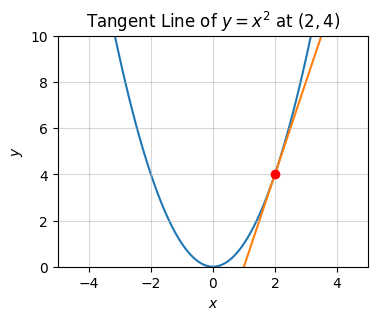
\includegraphics{notebooks/basic-calculus_files/figure-pdf/cell-8-output-1.png}

}

\end{figure}

Generally speaking, if the derivative at a point is \emph{positive} the
tangent line will slant towards the \emph{right}. If the derivative at
that point is \emph{negative} the tangent line will slant towards the
\emph{left}. If it's zero, the tangent line there will be horizontal.

The tangent line can be used to approximate the function \(y=f(x)\) when
\(x\) is close to \(x_0\). When \(x \approx x_0\), we can write

\[f(x) \approx f(x_0) + \frac{d}{dx}f(x_0)(x - x_0).\]

This is called a \textbf{first order approximation}, or the \textbf{best
linear approximation} to the function near \(x=x_0\). It turns out the
errors of this approximation are on the order of \((x-x_0)^2\), which
will usually be small provided \(x \approx x_0\).

\hypertarget{tangent-parabolas}{%
\subsubsection{Tangent Parabolas}\label{tangent-parabolas}}

The second derivative has a geometric interpretation as well. It
captures information about the \emph{curvature} of the function. To see
why this is true we need to look at \textbf{second order
approximations}, which extend first order approximations by adding a
quadratic term (shown in red),

\[f(x) \approx f(x_0) + \frac{d}{dx}f(x_0) (x-x_0) + \color{red}{\frac{1}{2}\frac{d^2}{dx^2}f(x_0) (x-x_0)^2}.\]

It seems weird there's a \(\frac{1}{2}\) in front of the quadratic term.
I won't go into detail on how this comes out. It relates to the fact
that differentiating \((x-x_0)^2\) brings a \(2\) out front, which kills
the \(\frac{1}{2}\). What's important is that this new term depends on
the second derivative at \(x=x_0\). This formula gives the \textbf{best
quadratic approximation} to \(y=f(x)\) near the point \(x=x_0\). Note
the error to this approximation turns out to be of the order of
\((x-x_0)^3\).

A second order approximation defines a \emph{tangent parabola} given by
a quadratic function \(y=ax^2+bx+c\), where \(a,b,c\) are coefficients
determined by the values of the inputs
\(f(x_0), \frac{d}{dx}f(x_0), \frac{d^2}{dx^2}f(x_0)\). Most
importantly, the leading coefficient \(a\) is just the second derivative
at \(x=x_0\), i.e.~\(a = \frac{d^2}{dx^2}f(x_0)\).

Since \(a\) determines the shape of the tangent parabola, it also
determines the curvature of the function at \(x=x_0\). If \(a\) is large
at \(x=x_0\), the function will be sharply curved around that point. If
\(a\) is small, the function will be very flat around \(x=x_0\). The
sign of \(a\) will indicate whether the function is curved upward or
downward. If \(a>0\) the function will be curved upward. If \(a < 0\)
it'll curve downward.

In our example \(y=x^2\), since \(a=\frac{d^2 y}{dx^2} = 2 > 0\),
meaning the tangent parabola is just the function \(y=x^2\) itself. Of
course it is. Since \(a\) is constant, the curvature for the parabola is
the same everywhere.

Since \(a=2>0\), the function \(y=x^2\) ``bowls upward'' everywhere.
Functions that ``bowl upward'' everywhere like this are called
\textbf{convex function}. If instead \(a < 0\) everywhere, e.g.~like it
would be for \(y=-x^2\), the function would ``bowl downward''
everywhere. These are called \textbf{convave functions}. Convex (and
concave) functions are very important for machine learning and
optimization more generally since they're guaranteed to have a unique
global minimum (or maximum). More on this in a future lesson.

Here's a more general example where the second derivative isn't
constant, \(y = \sin x\). In this case, \(\frac{dy}{dx} = \cos x\) and
\(\frac{d^2y}{dx^2} = -\sin x\). Suppose we want to get the tangent
parabola at the point \(x_0=-\frac{\pi}{2}\), so \(f(x_0)=-1\),
\(\frac{d}{dx}f(x_0)=0\) and \(\frac{d^2}{dx^2}f(x_0)=1\). Then the
tangent parabola is given by the equation

\[y = -1 + 0 \cdot \bigg(x + \frac{\pi}{2}\bigg) + \bigg(x + \frac{\pi}{2}\bigg)^2 = \bigg(x + \frac{\pi}{2}\bigg)^2 - 1.\]

This is an upward-sloping parabola with vertex at
\(\big(\frac{\pi}{2}, -1\big)\). Here's a plot of this idea. Notice how
the parabola approximates the function pretty well around the point
\(\big(\frac{\pi}{2}, -1\big)\), but gets less and less accurate as we
get away from that point. The fact that \(a=1\) here says that we should
expect an upward sloping parabola with ``unit curvature'', which is what
we see.

\begin{Shaded}
\begin{Highlighting}[]
\NormalTok{f }\OperatorTok{=} \KeywordTok{lambda}\NormalTok{ x: np.sin(x)}
\NormalTok{dfdx }\OperatorTok{=} \KeywordTok{lambda}\NormalTok{ x: np.cos(x)}
\NormalTok{d2fdx2 }\OperatorTok{=} \KeywordTok{lambda}\NormalTok{ x: }\OperatorTok{{-}}\NormalTok{np.sin(x)}

\NormalTok{x0 }\OperatorTok{=} \OperatorTok{{-}}\NormalTok{np.pi }\OperatorTok{/} \DecValTok{2}
\NormalTok{x }\OperatorTok{=}\NormalTok{ np.arange(}\OperatorTok{{-}}\DecValTok{5}\NormalTok{, }\DecValTok{5}\NormalTok{, }\FloatTok{0.1}\NormalTok{)}
\NormalTok{f\_parabola }\OperatorTok{=} \KeywordTok{lambda}\NormalTok{ x: f(x0) }\OperatorTok{+}\NormalTok{ dfdx(x0) }\OperatorTok{*}\NormalTok{ (x }\OperatorTok{{-}}\NormalTok{ x0) }\OperatorTok{+} \DecValTok{1}\OperatorTok{/}\DecValTok{2} \OperatorTok{*}\NormalTok{ d2fdx2(x0) }\OperatorTok{*}\NormalTok{ (x }\OperatorTok{{-}}\NormalTok{ x0) }\OperatorTok{**} \DecValTok{2}
\NormalTok{plot\_tangent\_curve(x, x0, f, f\_parabola, xlim}\OperatorTok{=}\NormalTok{(}\OperatorTok{{-}}\DecValTok{5}\NormalTok{, }\DecValTok{5}\NormalTok{), ylim}\OperatorTok{=}\NormalTok{(}\OperatorTok{{-}}\FloatTok{1.5}\NormalTok{, }\FloatTok{1.5}\NormalTok{), }
\NormalTok{                   title}\OperatorTok{=}\SpecialStringTok{f\textquotesingle{}Tangent Parabola of $y=\textbackslash{}sin x$ at $(\textbackslash{}pi/2, {-}1)$\textquotesingle{}}\NormalTok{)}
\end{Highlighting}
\end{Shaded}

\begin{figure}[H]

{\centering 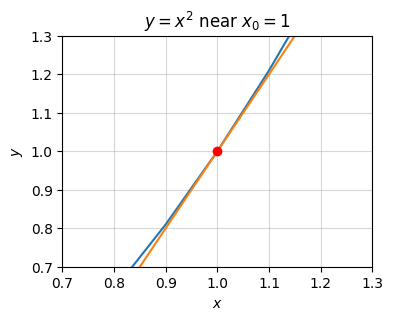
\includegraphics{notebooks/basic-calculus_files/figure-pdf/cell-9-output-1.png}

}

\end{figure}

\hypertarget{differentiation-rules}{%
\subsection{Differentiation Rules}\label{differentiation-rules}}

As we've seen, derivatives are also functions in and of themselves,
mapping inputs to outputs via \(\frac{dy}{dx} = \frac{d}{dx}f(x)\). For
this reason, several rules exist relating derivatives to their original
functions.

Here are the derivatives of some common functions that come up:

\begin{longtable}[]{@{}
  >{\raggedright\arraybackslash}p{(\columnwidth - 2\tabcolsep) * \real{0.4878}}
  >{\raggedright\arraybackslash}p{(\columnwidth - 2\tabcolsep) * \real{0.5122}}@{}}
\toprule()
\endhead
\textbf{Function} & \textbf{Derivative} \\
\(y = 0\) & \(\frac{dy}{dx} = 0\) \\
\(y = 1\) & \(\frac{dy}{dx} = 0\) \\
\(y = x\) & \(\frac{dy}{dx} = 1\) \\
\(y = x^2\) & \(\frac{dy}{dx} = 2x\) \\
\(y = \sqrt{x}\) & \(\frac{dy}{dx} = \frac{1}{2\sqrt{x}}\) \\
\(y = \frac{1}{x}\) & \(\frac{dy}{dx} = -\frac{1}{x^2}\) \\
\(y = e^x\) & \(\frac{dy}{dx} = e^x\) \\
\(y = \log{x}\) & \(\frac{dy}{dx} = \frac{1}{x}\) \\
\(y = \sin{x}\) & \(\frac{dy}{dx} = \cos{x}\) \\
\(y = \cos{x}\) & \(\frac{dy}{dx} = -\sin{x}\) \\
\(y = \sigma(x)\) &
\(\frac{dy}{dx} = \sigma(x)\big(1-\sigma(x)\big)\) \\
\(y = \tanh(x)\) & \(\frac{dy}{dx} = \big(1 - \tanh^2(x)\big)\) \\
\(y = \text{ReLU}(x)\) & \(\frac{dy}{dx} = u(x) = [x \geq 0]\) \\
\bottomrule()
\end{longtable}

Here are some more general derivative rules you can use to differentiate
more arbitrary functions:

\begin{longtable}[]{@{}
  >{\raggedright\arraybackslash}p{(\columnwidth - 4\tabcolsep) * \real{0.3030}}
  >{\raggedright\arraybackslash}p{(\columnwidth - 4\tabcolsep) * \real{0.3030}}
  >{\raggedright\arraybackslash}p{(\columnwidth - 4\tabcolsep) * \real{0.3939}}@{}}
\toprule()
\endhead
\textbf{Name} & \textbf{Rule} & \textbf{Example} \\
& \(\frac{d}{dx}(c) = 0\) for any constant \(c\) &
\(\frac{d}{dx}(10) = 0\) \\
Power Rule & \(\frac{d}{dx}x^n = nx^{n-1}\) for any \(n \neq 0\) &
\(\frac{d}{dx}x^3 = 3x^2\) \\
Addition Rule & \(\frac{d}{dx}(u + v) = \frac{du}{dx} + \frac{dv}{dx}\)
&
\(\frac{d}{dx}(x^2 + \log x) = \frac{d}{dx}x^2 + \frac{d}{dx}\log x = 2x + \frac{1}{x}\) \\
Constant Rule & \(\frac{d}{dx}(cy) = c \frac{dy}{dx}\) for any constant
\(c\) & \(\frac{d}{dx}2 \sin x = 2 \frac{d}{dx}\sin x = 2 \cos x\) \\
Product Rule & \(\frac{d}{dx}(uv)=u\frac{dv}{dx} + v\frac{du}{dx}\) &
\(\frac{d}{dx}(x e^x) = x \frac{d}{dx}e^x + e^x \frac{d}{dx} x = xe^x + e^x\) \\
Quotient Rule &
\(\frac{d}{dx}\big(\frac{u}{v}\big) = \frac{v\frac{du}{dx}-u\frac{dv}{dx}}{v^2}\)
&
\(\frac{d}{dx} \frac{\cos x}{x^2} = \frac{x^2\frac{d}{dx}\cos x-\cos x\frac{d}{dx}x^2}{(x^2)^2} = \frac{-x^2 \sin x - 2x \cos x}{x^4}\) \\
Chain Rule &
\(\frac{d}{dx}f(g(x)) = \frac{d}{dy}f(y)\frac{d}{dx}g(x) = \frac{dz}{dy}\frac{dy}{dx}\)
&
\(\frac{d}{dx} e^{\sin x} = \frac{d}{dy} e^y \frac{d}{dx}\sin x = e^{\sin x} \cos x\) \\
\bottomrule()
\end{longtable}

\hypertarget{the-chain-rule}{%
\subsubsection{The Chain Rule}\label{the-chain-rule}}

I want to call special attention to the \textbf{chain rule} since it's
probably the most important rule used in machine learning. Suppose we
have a composite function of two differentiable functions \(z=f(y)\) and
\(y=g(x)\). That is, \(z=f(g(x))\). Then the chain rule says that the
amount \(z\) changes in response to \(x\) changing by \(dx\) is,

\[\frac{dz}{dx} = \frac{dz}{dy}\frac{dy}{dx}.\]

\textbf{Proof:} Here's a quick proof of this fact. Perturb \(x\) by some
infinitesimal \(dx\). Then \(y + dy = g(x + dx)\), so

\[dy = g(x+dx)-g(x) = \frac{g(x+dx)-g(x)}{dx} dx = \frac{dy}{dx} dx.\]

Since \(dy\) is also infinitesimal, perturbing \(y\) by \(dy\) will do
the same thing to \(z=f(y)\), since \(z + dz = f(y + dy)\), and

\[dz = f(y+dy)-f(y) = \frac{f(y+dy)-f(y)}{dy} dy = \frac{dz}{dy} dy,\]

Putting these two results together, the infinitesimal change \(dz\) in
\(z=f(g(x))\) resulting from the original infinitesimal change \(dx\) is
given by

\[dz = \frac{dz}{dy} dy = \frac{dz}{dy} \frac{dy}{dx} dx.\]

Dividing both sides by \(dx\) gives the derivative of the composite
function \(z=f(g(x))\),

\[\frac{dz}{dx} = \frac{dz}{dy}\frac{dy}{dx}. \square\]

The chain rule extends to arbitrarily many compositions too. For
example, if we had a composition of four functions,

\begin{align*}
y &= f(x), \\
z &= g(y), \\
u &= h(z), \\
v &= i(u), \\
\end{align*}

the chain rule would say

\[\frac{dv}{dx} = \frac{dv}{du} \frac{du}{dz} \frac{dz}{dy} \frac{dy}{dx}.\]

This arbitrary \emph{chaining} is what allows us to differentiate
complex neural networks, where each \emph{layer} of the network is just
a function in this kind of chain.

\hypertarget{application-the-sigmoid-function}{%
\subsection{Application: The Sigmoid
Function}\label{application-the-sigmoid-function}}

To illustrate how to calculate derivatives I'll use a relevant example
to machine learning, the sigmoid function. Recall the sigmoid function
\(y=\sigma(x)\) is defined by

\[y = \frac{1}{1 + e^{-x}}.\]

Its shape looks like an S (hence the name), going from \(y=0\) at
\(x=-\infty\) to \(y=1\) at \(x=\infty\).

\begin{Shaded}
\begin{Highlighting}[]
\NormalTok{x }\OperatorTok{=}\NormalTok{ np.arange(}\OperatorTok{{-}}\DecValTok{10}\NormalTok{, }\DecValTok{10}\NormalTok{, }\FloatTok{0.1}\NormalTok{)}
\NormalTok{f }\OperatorTok{=} \KeywordTok{lambda}\NormalTok{ x:  }\DecValTok{1} \OperatorTok{/}\NormalTok{ (}\DecValTok{1} \OperatorTok{+}\NormalTok{ np.exp(}\OperatorTok{{-}}\NormalTok{x))}
\NormalTok{plot\_function(x, f, xlim}\OperatorTok{=}\NormalTok{(}\OperatorTok{{-}}\DecValTok{10}\NormalTok{, }\DecValTok{10}\NormalTok{), ylim}\OperatorTok{=}\NormalTok{(}\OperatorTok{{-}}\FloatTok{0.5}\NormalTok{, }\FloatTok{1.5}\NormalTok{), ticks\_every}\OperatorTok{=}\NormalTok{[}\DecValTok{5}\NormalTok{, }\FloatTok{0.5}\NormalTok{], title}\OperatorTok{=}\StringTok{\textquotesingle{}Sigmoid Function\textquotesingle{}}\NormalTok{)}
\end{Highlighting}
\end{Shaded}

\begin{figure}[H]

{\centering \includegraphics{notebooks/basic-calculus_files/figure-pdf/cell-10-output-1.png}

}

\end{figure}

Let's calculate the derivative of this function. First, though, let's
use some intuition and try to figure out what the derivative should be
doing based on the shape of the sigmoid curve. When \(x\) is really
negative, say \(x < -5\), the slope looks basically flat, hence the
derivative should be zero there. Similarly, when \(x\) is really
positive, say \(x > 5\), the derivative should be zero there too. Around
\(x=0\), say \(-1 < x < 1\), the sigmoid looks kind of linear with
positive slope. There we should expect the derivative to be positive,
and roughly constant over that interval.

To verify this, let's calculate the derivative of the sigmoid
explicitly. There are a few ways to do this, but I'll use the chain rule
here. We have

\begin{align}
\frac{d}{dx} \sigma(x) &= \frac{d}{dx} \frac{1}{1 + e^{-x}}\\
&= \frac{d}{dx} (1 + e^{-x})^{-1} \\
&= (-1) (1 + e^{-x})^{-2} \frac{d}{dx} e^{-x} \\
&= -(1 + e^{-x})^{-2} (-1) e^{-x} \\
&= \frac{e^{-x}}{(1 + e^{-x})^{2}} \\
&= \frac{1}{1 + e^{-x}} \frac{(1 + e^{-x}) - 1}{1 + e^{-x}} \\
&= \frac{1}{1 + e^{-x}} \bigg(1-\frac{1}{1 + e^{-x}}\bigg) \\
&= \sigma(x) \big(1 - \sigma(x)\big).
\end{align}

Let's look at this answer and verify it matches our intuition as to what
the derivative of the sigmoid should be.

\begin{itemize}
\tightlist
\item
  When \(x < -5\), \(\sigma(x) \approx 0\), hence
  \(\frac{d}{dx} \sigma(x) \approx 0\).
\item
  When \(x > 5\), \(\sigma(x) \approx 1\), so
  \(1 - \sigma(x) \approx 0\), and again
  \(\frac{d}{dx} \sigma(x) \approx 0\).
\item
  When \(-1 < x < 1\),
  \(\sigma(x) \approx \sigma(0) + \frac{d}{dx}\sigma(0) \cdot (x-0) = \frac{1}{2} + \frac{1}{2}\big(1 - \frac{1}{2}\big) \cdot x = \frac{1}{2} + \frac{1}{4}x\),
  which is a tangent line with a positive slope of \(\frac{1}{4}\).
\end{itemize}

To further verify the things look like a line around \(x=0\), we could
look at the second derivative and verify it's approximately zero in the
region \(-1 < x < 1\). I'll leave that exercise to you.

The sigmoid function shows up in machine learning when doing binary
classification. If a problem can be classified into two classes, \(0\)
or \(1\), the sigmoid can be used to model the probability of the input
being in class \(1\). The closer the sigmoid is to \(1\), or
equivalently the larger \(x\) is, the more likely the input is a \(1\).
More on this in a future lesson.

To calculate the derivative of a function in sympy, use
\texttt{y.diff(x)}, which means ``differentiate \(y\) with respect to
\(x\)''.

Here is a calculation of the derivative of the sigmoid function. I'll
also calculate the second derivative to show you how easy it is to do
relative to the torture of trying to do it by hand.

\begin{Shaded}
\begin{Highlighting}[]
\NormalTok{x }\OperatorTok{=}\NormalTok{ sp.Symbol(}\StringTok{\textquotesingle{}x\textquotesingle{}}\NormalTok{)}
\NormalTok{y }\OperatorTok{=} \DecValTok{1} \OperatorTok{/}\NormalTok{ (}\DecValTok{1} \OperatorTok{+}\NormalTok{ sp.exp(}\OperatorTok{{-}}\NormalTok{x))}
\NormalTok{dydx }\OperatorTok{=}\NormalTok{ y.diff(x)}
\NormalTok{d2dx2 }\OperatorTok{=}\NormalTok{ y.diff(x).diff(x)}
\BuiltInTok{print}\NormalTok{(}\SpecialStringTok{f\textquotesingle{}y = }\SpecialCharTok{\{}\NormalTok{y}\SpecialCharTok{\}}\SpecialStringTok{\textquotesingle{}}\NormalTok{)}
\BuiltInTok{print}\NormalTok{(}\SpecialStringTok{f\textquotesingle{}dydx = }\SpecialCharTok{\{}\NormalTok{dydx}\SpecialCharTok{\}}\SpecialStringTok{\textquotesingle{}}\NormalTok{)}
\BuiltInTok{print}\NormalTok{(}\SpecialStringTok{f\textquotesingle{}d2dx2 = }\SpecialCharTok{\{}\NormalTok{d2dx2}\SpecialCharTok{\}}\SpecialStringTok{\textquotesingle{}}\NormalTok{)}
\end{Highlighting}
\end{Shaded}

\begin{verbatim}
y = 1/(1 + exp(-x))
dydx = exp(-x)/(1 + exp(-x))**2
d2dx2 = -exp(-x)/(1 + exp(-x))**2 + 2*exp(-2*x)/(1 + exp(-x))**3
\end{verbatim}

\hypertarget{integration}{%
\section{Integration}\label{integration}}

Since integration is literally half of the subject of calculus, I owe it
to at least briefly mention the topic. This section is only really
applicable to the other topics in this book if you want to better
understand probability distributions, something I'll cover in detail in
the next lesson. If you don't mind thinking of probability distributions
as histograms with infinitely many samples, you're free to skip this
section and move ahead.

\hypertarget{summing-infinitesimals}{%
\subsection{Summing Infinitesimals}\label{summing-infinitesimals}}

The other half of calculus is essentially about summing up small things
to get big things. By small things of course I mean infinitesimals.
Suppose we have a bunch of infinitesimals
\(\varepsilon_0, \varepsilon_1, \cdots, \varepsilon_{n-1}\). We can add
them together to get a new infinitesimal
\(\varepsilon_0 + \varepsilon_1 + \cdots + \varepsilon_{n-1}\).

Suppose we want to add up the same infinitesimal \(\varepsilon\) some
number \(N\) times,
\[\underbrace{\varepsilon + \varepsilon + \cdots + \varepsilon}_{\text{N times}} = N\varepsilon.\]

If \(N\) is any reasonably sized finite number, say a number like
\(N=1000\), then the product \(N\varepsilon\) will again be
infinitesimal, since \((N\varepsilon)^2 \approx 0\). But if we make
\(N\) \emph{infinitely large}, then \(N\varepsilon\) will be a finite
number.

Here's how this might look when adopting our informal convention that
infinitesimals equal \(10^{-300}\) and infinitely large numbers equal
\(10^{300}\). For \(N=1000\) the square \((N\varepsilon)^2 \approx 0\).
But it's not when we take \(N=10^{300}\). It's finite, with
\((N\varepsilon)^2=1\).

\begin{Shaded}
\begin{Highlighting}[]
\NormalTok{epsilon }\OperatorTok{=} \FloatTok{1e{-}300}

\NormalTok{N }\OperatorTok{=} \DecValTok{1000}
\BuiltInTok{print}\NormalTok{(}\SpecialStringTok{f\textquotesingle{}N = }\SpecialCharTok{\{}\NormalTok{N}\SpecialCharTok{\}}\SpecialStringTok{\textquotesingle{}}\NormalTok{)}
\BuiltInTok{print}\NormalTok{(}\SpecialStringTok{f\textquotesingle{}(N * epsilon)\^{}2 = }\SpecialCharTok{\{}\NormalTok{(N }\OperatorTok{*}\NormalTok{ epsilon) }\OperatorTok{**} \DecValTok{2}\SpecialCharTok{\}}\SpecialStringTok{\textquotesingle{}}\NormalTok{)}

\NormalTok{N }\OperatorTok{=} \FloatTok{1e300}
\BuiltInTok{print}\NormalTok{(}\SpecialStringTok{f\textquotesingle{}N = }\SpecialCharTok{\{}\NormalTok{N}\SpecialCharTok{\}}\SpecialStringTok{\textquotesingle{}}\NormalTok{)}
\BuiltInTok{print}\NormalTok{(}\SpecialStringTok{f\textquotesingle{}(N * epsilon)\^{}2 = }\SpecialCharTok{\{}\NormalTok{(N }\OperatorTok{*}\NormalTok{ epsilon) }\OperatorTok{**} \DecValTok{2}\SpecialCharTok{\}}\SpecialStringTok{\textquotesingle{}}\NormalTok{)}
\end{Highlighting}
\end{Shaded}

\begin{verbatim}
N = 1000
(N * epsilon)^2 = 0.0
N = 1e+300
(N * epsilon)^2 = 1.0
\end{verbatim}

Thus, if we add up only a \emph{finite} number of infinitesimals we'll
again get an \emph{infinitesimal}. But, if we add up an \emph{infinitely
large} number of infinitesimals we'll get something \emph{finite}. This
is the idea behind integration.

\hypertarget{area-under-the-curve}{%
\subsection{Area Under The Curve}\label{area-under-the-curve}}

Let's do an example. Suppose we're interested in calculating the area
under the curve \(y=\sqrt{x}\) between two points, say \(x=0\) and
\(x=10\). How would we go about this?

\begin{Shaded}
\begin{Highlighting}[]
\NormalTok{f }\OperatorTok{=} \KeywordTok{lambda}\NormalTok{ x: np.sqrt(x)}
\NormalTok{x }\OperatorTok{=}\NormalTok{ np.linspace(}\DecValTok{0}\NormalTok{, }\DecValTok{10}\NormalTok{, }\DecValTok{100}\NormalTok{)}
\NormalTok{a, b }\OperatorTok{=} \DecValTok{0}\NormalTok{, }\DecValTok{10}
\NormalTok{plot\_function\_with\_area(x, f, a}\OperatorTok{=}\NormalTok{a, b}\OperatorTok{=}\NormalTok{b, title}\OperatorTok{=}\StringTok{\textquotesingle{}Area Under $y=\textbackslash{}sqrt}\SpecialCharTok{\{x\}}\StringTok{$ Between $0 \textbackslash{}leq x \textbackslash{}leq 10$\textquotesingle{}}\NormalTok{)}
\end{Highlighting}
\end{Shaded}

\begin{figure}[H]

{\centering \includegraphics{notebooks/basic-calculus_files/figure-pdf/cell-13-output-1.png}

}

\end{figure}

Perhaps the easiest idea is to approximate the function by a shape
that's easier to calculate the area of, something you've seen in
geometry, like a square or a triangle. A better idea is to take a bunch
of simple shapes, calculate their areas, and add them together.

Let's try to do this using rectangles. Let's approximate the function
\(f(x)=\sqrt{x}\) with \(N=10\) equally-spaced rectangles of varying
heights \(f(x)\), where \(x\) is taken at each integer value
\(x=1,2,3,\cdots,10\). The width of each rectangle is
\(dx=\frac{b-a}{N}=1\). We know for rectangles their area is width times
height, which in this case is \(dx \cdot f(x) = f(x)dx\). Then the total
area under the curve of \(y=\sqrt{x}\) would roughly be the sum of all
these rectangle areas,

\begin{align}
A &\approx f(1)dx + f(2)dx + f(3)dx + \cdots + f(10)dx \\
&= \big(f(1) + f(2) + f(3) + \cdots + f(10)\big)\cdot dx \\
&= \big(\sqrt{1} + \sqrt{2} + \sqrt{3} + \cdots + \sqrt{10}\big)\cdot 1 \\
&\approx 22.468
\end{align}

Let's visualize what's going on. This plot shows both the curve and its
approximating rectangles. It also prints out the approximating area
calculated above.

\begin{Shaded}
\begin{Highlighting}[]
\NormalTok{plot\_approximating\_rectangles(x, f, dx}\OperatorTok{=}\FloatTok{1.0}\NormalTok{)}
\end{Highlighting}
\end{Shaded}

\begin{verbatim}
Approximate Area: 22.468278186204103
\end{verbatim}

\begin{figure}[H]

{\centering 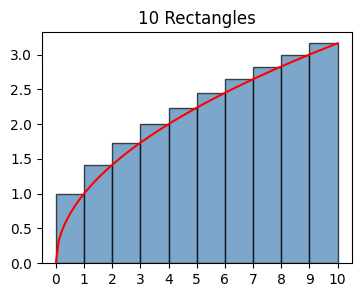
\includegraphics{notebooks/basic-calculus_files/figure-pdf/cell-14-output-2.png}

}

\end{figure}

If you stare at the plot you can see our area estimate is okay but not
great. The rectangles are \emph{overestimating} the area under the curve
since they all have segments of area lying above the curve.

The problem was that the rectangles we used were too coarse. It's better
to use narrower rectangles, and more of them. What we need to do is make
\(dx\) smaller by making \(N\) bigger. Let's try using \(N=50\)
rectangles of width \(dx=0.2\) instead and see how much the result
improves.

\begin{Shaded}
\begin{Highlighting}[]
\NormalTok{plot\_approximating\_rectangles(x, f, dx}\OperatorTok{=}\FloatTok{0.2}\NormalTok{)}
\end{Highlighting}
\end{Shaded}

\begin{verbatim}
Approximate Area: 21.380011968222313
\end{verbatim}

\begin{figure}[H]

{\centering 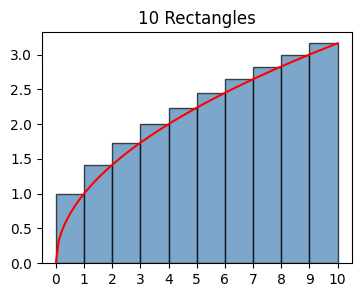
\includegraphics{notebooks/basic-calculus_files/figure-pdf/cell-15-output-2.png}

}

\end{figure}

It looks better. We're at \(21.380\) now. If you zoom in you'll see
we're still overestimating the true area, but not by near as much as
before. As we make \(dx\) smaller and smaller, and \(N\) bigger and
bigger, this estimate will get better and better.

The exact area under this curve turns out to be

\[A = \frac{20}{3}\sqrt{10} \approx 21.082.\]

This will be the case when the rectangles are infinitesimally thin, so
thin that the errors disappear and the area calculation becomes exact.

Let's try to calculate the approximating areas using smaller and smaller
rectangles and see how close we can get to the exact answer. To do this,
I'll use a loop to calculate the area for successively smaller values of
\(dx\).

\begin{Shaded}
\begin{Highlighting}[]
\NormalTok{f }\OperatorTok{=} \KeywordTok{lambda}\NormalTok{ x: np.sqrt(x)}

\ControlFlowTok{for}\NormalTok{ dx }\KeywordTok{in}\NormalTok{ [}\DecValTok{1}\NormalTok{, }\FloatTok{0.1}\NormalTok{, }\FloatTok{0.01}\NormalTok{, }\FloatTok{0.001}\NormalTok{, }\FloatTok{0.0001}\NormalTok{]:}
\NormalTok{    N }\OperatorTok{=} \BuiltInTok{int}\NormalTok{(}\DecValTok{10} \OperatorTok{/}\NormalTok{ dx)}
\NormalTok{    xs }\OperatorTok{=}\NormalTok{ np.cumsum(dx }\OperatorTok{*}\NormalTok{ np.ones(N))}
\NormalTok{    area }\OperatorTok{=}\NormalTok{ np.}\BuiltInTok{sum}\NormalTok{([f(x)}\OperatorTok{*}\NormalTok{dx }\ControlFlowTok{for}\NormalTok{ x }\KeywordTok{in}\NormalTok{ xs])}
    \BuiltInTok{print}\NormalTok{(}\SpecialStringTok{f\textquotesingle{}N = }\SpecialCharTok{\{}\NormalTok{N}\SpecialCharTok{:6d\}}\SpecialStringTok{ }\CharTok{\textbackslash{}t}\SpecialStringTok{ dx = }\SpecialCharTok{\{}\NormalTok{dx}\SpecialCharTok{:8.4f\}}\SpecialStringTok{ }\CharTok{\textbackslash{}t}\SpecialStringTok{ A = }\SpecialCharTok{\{}\NormalTok{area}\SpecialCharTok{:4f\}}\SpecialStringTok{\textquotesingle{}}\NormalTok{)}
\end{Highlighting}
\end{Shaded}

\begin{verbatim}
N =     10   dx =   1.0000   A = 22.468278
N =    100   dx =   0.1000   A = 21.233523
N =   1000   dx =   0.0100   A = 21.097456
N =  10000   dx =   0.0010   A = 21.083426
N = 100000   dx =   0.0001   A = 21.082009
\end{verbatim}

It looks like if we want to get the correct answer \(21.082\) to 3
decimal places we'd need to use \(N=100000\) rectangles of width
\(dx=10^{-4}\). In practice that's an awful lot of terms to sum up.
There are better ways to actually calculate these things numerically
than just using the above definition
(e.g.~\href{https://en.wikipedia.org/wiki/Simpson\%27s_rule}{Simpson's
Rule}), but I won't go into those.

Let's generalize this. Suppose we want to calculate the area under the
curve of some function \(y=f(x)\) between two points \(x=a\) and
\(x=b\). We can do this by taking \(N\) rectangles each of width
\(dx=\frac{b-a}{N}\) and height \(f(x)dx\) and summing up their areas.
If \(x_0,x_1,\cdots,x_{N-1}\) are the points we're evaluating the
heights at, then
\[A \approx f(x_0)dx + f(x_1)dx + f(x_2)dx + \cdots + f(x_{N-1})dx = \sum_{n=0}^{N-1} f(x_n) dx.\]

To get the exact area, let's allow \(N\) to get infinitely large, which
also means \(dx\) will become infinitesimal. When we do this, it's
conventional to use a different symbol for the sum, the long-S symbol
\(\int\). Instead of writing

\[A = \sum_{n=0}^{N-1} f(x_n) dx,\]

we'd write \[A = \int_a^{b} f(x) dx.\]

Read this as ``the integral from 0 to 10 of \(f(x)dx\)''. It's called
the \textbf{definite integral} of the function. In our example, this
would be

\[A = \int_0^{10} \sqrt{x} dx.\]

Of course, this fancy notation doesn't actually tell us anything new.
We're still just summing up the areas of a bunch of rectangles.

\hypertarget{integration-rules}{%
\subsection{Integration Rules}\label{integration-rules}}

It's not at all clear from this definition how we'd get the \emph{exact}
answer \(A=\frac{20}{3}\sqrt{10}\) shown above. We can get to it
approximately by summing rectangle areas, but if we want to get the
exact value we'll need a few integral rules.

Before doing so I need to talk about the \textbf{indefinite integral},
sometimes called the antiderivative. If \(f(x)\) is some function, then
its indefinite integral is some other function \(F(x)\) whose derivative
is \(f(x)\), \[f(x) = \frac{d}{dx} F(x).\]

Typically the indefinite integral is written as an integral, but without
limits of integration shown,

\[F(x) = \int f(x) dx.\]

To evaluate a typical \emph{definite} integral like \(\int_a^b f(x) dx\)
the rule is
\[\int_a^b f(x) dx = F(x) \bigg|_{x=a}^{x=b} = F(b) - F(a).\]

That is, we first calculate the indefinite integral \(F(x)\), then
evaluate it at the points \(a\) and \(b\), then subtract their
difference to get the definite integral, which itself is just the area
under the curve of \(f(x)\). The fact we can think of areas under curves
in terms of another function like this is not obvious. It follows from
the \textbf{Fundamental Theorem of Calculus}, which I won't try to prove
here.

With this out of the way, here are some common indefinite integrals.
Note we can add a constant \(c\) to each of these and the answer would
still be the same. I'll state them in the standard form where \(c=0\).

\begin{longtable}[]{@{}
  >{\raggedright\arraybackslash}p{(\columnwidth - 2\tabcolsep) * \real{0.4878}}
  >{\raggedright\arraybackslash}p{(\columnwidth - 2\tabcolsep) * \real{0.5122}}@{}}
\toprule()
\endhead
\textbf{Function} & \textbf{Integral} \\
\(y = 0\) & \(\int y dx = 0\) \\
\(y = 1\) & \(\int y dx = x\) \\
\(y = x\) & \(\int y dx = \frac{1}{2}x^2\) \\
\(y = x^2\) & \(\int y dx = \frac{1}{3}x^3\) \\
\(y = \sqrt{x}\) & \(\int y dx = \frac{2}{3} x^{3/2}\) \\
\(y = \frac{1}{x}\) & \(\int y dx = \log{x}\) \\
\(y = e^x\) & \(\int y dx = e^x\) \\
\(y = \log{x}\) & \(\int y dx = x \log{x} - x\) \\
\(y = \sin{x}\) & \(\int y dx = -\cos{x}\) \\
\(y = \cos{x}\) & \(\int y dx = \sin{x}\) \\
\bottomrule()
\end{longtable}

Here are a few more general integral rules:

\begin{longtable}[]{@{}
  >{\raggedright\arraybackslash}p{(\columnwidth - 4\tabcolsep) * \real{0.3030}}
  >{\raggedright\arraybackslash}p{(\columnwidth - 4\tabcolsep) * \real{0.3030}}
  >{\raggedright\arraybackslash}p{(\columnwidth - 4\tabcolsep) * \real{0.3939}}@{}}
\toprule()
\endhead
\textbf{Name} & \textbf{Rule} & \textbf{Example} \\
Fundamental Theorem of Calculus & \(\int_a^b f(x) dx = F(b) - F(a)\)
where \(\frac{d}{dx}F(x) = f(x)\) &
\(\int_0^1 x dx = \frac{1}{2} x^2 \big |_0^1 = \frac{1}{2} 1^2 - \frac{1}{2} 0^2 = \frac{1}{2}\) \\
Reversing Limits of Integration & \(\int_b^a y dx = -\int_a^b y dx\) &
\(\int_2^0 1 dx = -\int_0^2 1 dx = 2\) \\
Splitting Up Limits of Integration &
\(\int_a^b y dx = \int_a^c y dx + \int_c^d y dx\) &
\(\int_0^2 1 dx = \int_0^1 1 dx + \int_1^2 1 dx = 1 + (2-1) = 2\) \\
Power Rule & \(\int x^n dx = \frac{1}{n+1}x^{n+1}\) for any
\(n \neq -1\) &
\(\int x^{-2} dx = \frac{1}{-2+1}x^{-2+1} = -\frac{1}{x}\) \\
Addition Rule & \(\int (u + v) dx = \int u dx + \int v dx\) &
\(\int (1 + e^x) dx = \int 1 dx + \int e^x dx = x + e^x\) \\
Constant Rule & \(\int cy dx = c \int y dx\) &
\(\int 5 \cos{x} dx = 5 \int \cos{x} dx = 5 \sin{x}\) \\
Integration By Parts & \(\int u dv = uv - \int v du\) &
\(\int x e^x dx = \int x d(e^x) = x e^x - \int e^x dx = x e^x - e^x\) \\
Leibniz Rule & \(\frac{d}{dx} \int y dx = y\) &
\(\frac{d}{dx} \int_0^x \sin t dt = \sin x\) \\
Change of Variables & \(\int f(u) du = \int f(u(x)) \frac{du}{dx} dx\) &
\(\int x e^{x^2} dx = \int e^{x^2} d\big(\frac{1}{2}x^2\big) = \frac{1}{2} \int e^u du = \frac{1}{2} e^u = \frac{1}{2} e^{x^2}\) \\
\bottomrule()
\end{longtable}

Note \(d(f(x))\) is just the differential form of the derivative
\(\frac{d}{dx}f(x)\), so \(d(f(x)) = \frac{d}{dx}f(x) dx\).

It's worth mentioning that integral rules are often much harder to apply
than derivative rules. In fact, it's not even possible to symbolically
integrate every function. The Gaussian function \(y=e^{-x^2}\) is a
well-known example of a function that can't be integrated symbolically.
Of course, we can \emph{always} calculate the \emph{definite} integral
numerically, even if we can't symbolically.

Just as with derivatives, sympy can evaluate integrals for you, both
definite and indefinite integrals. Below I'll use
\texttt{y.integrate((x,\ 0,\ 10))} to calculate the area under the curve
problem I did before,

\[A = \int_0^{10} \sqrt{x} dx = \frac{20}{3} \sqrt{10}.\]

Sympy can of course handle indefinite integrals too by leaving off the
limits of integration.

\begin{Shaded}
\begin{Highlighting}[]
\NormalTok{x }\OperatorTok{=}\NormalTok{ sp.Symbol(}\StringTok{\textquotesingle{}x\textquotesingle{}}\NormalTok{)}
\NormalTok{y }\OperatorTok{=}\NormalTok{ sp.sqrt(x)}
\NormalTok{A }\OperatorTok{=}\NormalTok{ y.integrate((x, }\DecValTok{0}\NormalTok{, }\DecValTok{10}\NormalTok{))}
\NormalTok{y\_int }\OperatorTok{=}\NormalTok{ y.integrate(x)}
\BuiltInTok{print}\NormalTok{(}\SpecialStringTok{f\textquotesingle{}y = }\SpecialCharTok{\{}\NormalTok{y}\SpecialCharTok{\}}\SpecialStringTok{\textquotesingle{}}\NormalTok{)}
\BuiltInTok{print}\NormalTok{(}\SpecialStringTok{f\textquotesingle{}A = }\SpecialCharTok{\{}\NormalTok{A}\SpecialCharTok{\}}\SpecialStringTok{\textquotesingle{}}\NormalTok{)}
\BuiltInTok{print}\NormalTok{(}\SpecialStringTok{f\textquotesingle{}int y dx = }\SpecialCharTok{\{}\NormalTok{y}\SpecialCharTok{.}\NormalTok{integrate(x)}\SpecialCharTok{\}}\SpecialStringTok{\textquotesingle{}}\NormalTok{)}
\end{Highlighting}
\end{Shaded}

\begin{verbatim}
y = sqrt(x)
A = 20*sqrt(10)/3
int y dx = 2*x**(3/2)/3
\end{verbatim}

\hypertarget{limits}{%
\section{Limits}\label{limits}}

Yet another application of infinitesimals is to look at the nearby
behavior of a function around some point. Suppose we have some function
\(y=f(x)\). We'd like to look at the nearby behavior of the function
around some point \(x=x_0\). If you like, think of \(x\) as being so
close to \(x_0\) that the first order approximation applies almost
exactly,

\[f(x) \approx f(x_0) + \frac{d}{dx}f(x_0) (x-x_0).\]

Pick a point \(x\) that's infinitesimally close to \(x_0\), so
\(x \approx x_0\), yet \(x \neq x_0\) exactly. If \(f(x) \approx L\), we
say \(L\) is the \textbf{limit} as \(x\) approaches \(x_0\), and write

\[L = \lim_{x \rightarrow x_0} f(x).\]

More formally, say \(L\) is the limit if the difference
\(|f(x_0+\varepsilon)-L|\) is infinitesimal whenever \(\varepsilon\) is
infinitesimal. Another notation for the limit is

\[y \rightarrow L \text{ as } x \rightarrow x_0.\]

\hypertarget{continuity}{%
\subsubsection{Continuity}\label{continuity}}

This all seems kind of pedantic if you think about it. It seems like
we're doing a bunch of extra work just to evaluate the function at
\(x_0\), which of course would imply \(L=f(x_0)\). In most practical
cases this is true, but not \emph{always}.

A classic example is a function with a hole in it. Suppose we have a
function \(y=f(x)\) like this

\[
y = 
\begin{cases}
1 & x = 0, \\
x^2 & x \neq 0.
\end{cases}
\]

Here's what it looks like. It's just a parabola \(y=x^2\), but with a
hole at \(x=0\) since \(f(0)=1\neq 0^2\).

\begin{Shaded}
\begin{Highlighting}[]
\NormalTok{x }\OperatorTok{=}\NormalTok{ np.arange(}\OperatorTok{{-}}\DecValTok{2}\NormalTok{, }\DecValTok{2}\NormalTok{, }\FloatTok{0.01}\NormalTok{)}
\NormalTok{f\_neq\_0 }\OperatorTok{=} \KeywordTok{lambda}\NormalTok{ x: x }\OperatorTok{**} \DecValTok{2}

\NormalTok{plt.plot(x, f\_neq\_0(x), color}\OperatorTok{=}\StringTok{\textquotesingle{}red\textquotesingle{}}\NormalTok{, zorder}\OperatorTok{=}\DecValTok{0}\NormalTok{)}
\NormalTok{plt.scatter(}\DecValTok{0}\NormalTok{, }\DecValTok{1}\NormalTok{, color}\OperatorTok{=}\StringTok{\textquotesingle{}red\textquotesingle{}}\NormalTok{, marker}\OperatorTok{=}\StringTok{\textquotesingle{}o\textquotesingle{}}\NormalTok{, s}\OperatorTok{=}\DecValTok{20}\NormalTok{, zorder}\OperatorTok{=}\DecValTok{1}\NormalTok{)}
\NormalTok{plt.scatter(}\DecValTok{0}\NormalTok{, }\DecValTok{0}\NormalTok{, c}\OperatorTok{=}\StringTok{\textquotesingle{}white\textquotesingle{}}\NormalTok{, edgecolors}\OperatorTok{=}\StringTok{\textquotesingle{}red\textquotesingle{}}\NormalTok{, marker}\OperatorTok{=}\StringTok{\textquotesingle{}o\textquotesingle{}}\NormalTok{, s}\OperatorTok{=}\DecValTok{20}\NormalTok{, zorder}\OperatorTok{=}\DecValTok{2}\NormalTok{)}
\NormalTok{plt.grid(}\VariableTok{True}\NormalTok{, alpha}\OperatorTok{=}\FloatTok{0.5}\NormalTok{)}
\NormalTok{plt.xlabel(}\StringTok{\textquotesingle{}x\textquotesingle{}}\NormalTok{)}
\NormalTok{plt.ylabel(}\StringTok{\textquotesingle{}y\textquotesingle{}}\NormalTok{)}
\NormalTok{plt.title(}\StringTok{\textquotesingle{}$y = 1$ if $x = 0$ else $x\^{}2$\textquotesingle{}}\NormalTok{)}
\NormalTok{plt.show()}
\end{Highlighting}
\end{Shaded}

\begin{figure}[H]

{\centering \includegraphics{notebooks/basic-calculus_files/figure-pdf/cell-18-output-1.png}

}

\end{figure}

Let's try to find the limit of this function at \(x_0=0\). Pick an \(x\)
close to \(0\), but not exactly \(0\), say \(x=\varepsilon\), where
\(\varepsilon\) is infinitesimal. Then we'd have

\[L = \lim_{x \rightarrow 0} f(x) = f(\varepsilon) = \varepsilon^2 \approx 0.\]

But \(f(0) = 1\), which means the limit at \(x=0\) is \emph{not} the
value of the function at \(x=0\). This is just a long, drawn-out way of
saying that the limit is what the function \emph{would} be if it didn't
have a hole in it at \(x=0\).

A function that \emph{is} well-behaved in this sense that it has no
holes or jumps is called \textbf{continuous}. Continuous functions
satisfy the very nice property that the limit can be pulled inside the
function,

\[\lim_{x \rightarrow x_0} f(x) = f\bigg(\lim_{x \rightarrow x_0} x\bigg) = f(x_0).\]

Since almost every function we work with in practice is continuous, we
can by and large take for granted that we can do this, at least at
almost all points we evaluate the function at, but keeping in mind that
exceptions do occur and you sometimes have to be careful.

\hypertarget{infinite-limits}{%
\subsubsection{Infinite Limits}\label{infinite-limits}}

In my experience, the only real place limits seem to come up in machine
learning is the infinite limit case when \(x \rightarrow \infty\). In
that case, we have

\[\lim_{x \rightarrow \infty} f(x) \approx f(N),\]

where \(N\) is infinitely large. The easiest way to figure these limits
out is to plug in a large values for \(x\) and see what \(f(x)\) is
tending towards as \(x\) gets large. As an example, let's try to find
the limit of \(y=e^{-x}\) as \(x \rightarrow \infty\). Here's what the
function looks like. It seems to rapidly decay to \(0\) as \(x\) gets
large. Not even large. It's basically at \(y \approx 0\) by the time
\(x=10\).

\begin{Shaded}
\begin{Highlighting}[]
\NormalTok{x }\OperatorTok{=}\NormalTok{ np.arange(}\DecValTok{0}\NormalTok{, }\DecValTok{10}\NormalTok{, }\FloatTok{0.1}\NormalTok{)}
\NormalTok{f }\OperatorTok{=} \KeywordTok{lambda}\NormalTok{ x:  np.exp(}\OperatorTok{{-}}\NormalTok{x)}
\NormalTok{plot\_function(x, f, xlim}\OperatorTok{=}\NormalTok{(}\OperatorTok{{-}}\FloatTok{0.5}\NormalTok{, }\DecValTok{10}\NormalTok{), ylim}\OperatorTok{=}\NormalTok{(}\OperatorTok{{-}}\FloatTok{0.5}\NormalTok{, }\FloatTok{1.5}\NormalTok{), ticks\_every}\OperatorTok{=}\VariableTok{None}\NormalTok{, title}\OperatorTok{=}\StringTok{\textquotesingle{}$y=e\^{}\{{-}x\}$\textquotesingle{}}\NormalTok{)}
\end{Highlighting}
\end{Shaded}

\begin{figure}[H]

{\centering \includegraphics{notebooks/basic-calculus_files/figure-pdf/cell-19-output-1.png}

}

\end{figure}

Let's pick successively large values of \(x\) and see if we can identify
the limit numerically. I'll choose \(x=e^0, e^1, \cdots, e^5\). You can
see that numerically speaking \(y=e^{-x}\) is pretty much \(0\) by the
time \(x=20\). This suggests the limit is \(L=0\) as
\(x \rightarrow \infty\). While this isn't a ``proof'', it should be
pretty convincing.

\begin{Shaded}
\begin{Highlighting}[]
\ControlFlowTok{for}\NormalTok{ x }\KeywordTok{in}\NormalTok{ np.exp(}\BuiltInTok{range}\NormalTok{(}\DecValTok{6}\NormalTok{)):}
\NormalTok{    y }\OperatorTok{=}\NormalTok{ np.exp(}\OperatorTok{{-}}\NormalTok{x)}
    \BuiltInTok{print}\NormalTok{(}\SpecialStringTok{f\textquotesingle{}x = }\SpecialCharTok{\{}\NormalTok{x}\SpecialCharTok{.}\BuiltInTok{round}\NormalTok{(}\DecValTok{2}\NormalTok{)}\SpecialCharTok{\}}\SpecialStringTok{ }\CharTok{\textbackslash{}t}\SpecialStringTok{ y = }\SpecialCharTok{\{}\NormalTok{y}\SpecialCharTok{.}\BuiltInTok{round}\NormalTok{(}\DecValTok{8}\NormalTok{)}\SpecialCharTok{\}}\SpecialStringTok{\textquotesingle{}}\NormalTok{)}
\end{Highlighting}
\end{Shaded}

\begin{verbatim}
x = 1.0      y = 0.36787944
x = 2.72     y = 0.06598804
x = 7.39     y = 0.00061798
x = 20.09    y = 0.0
x = 54.6     y = 0.0
x = 148.41   y = 0.0
\end{verbatim}

If you like, you can also use sympy to evaluate the infinite limit
symbolically.

\begin{Shaded}
\begin{Highlighting}[]
\NormalTok{x }\OperatorTok{=}\NormalTok{ sp.symbols(}\StringTok{\textquotesingle{}x\textquotesingle{}}\NormalTok{)}
\NormalTok{y }\OperatorTok{=}\NormalTok{ sp.exp(}\OperatorTok{{-}}\NormalTok{x)}
\NormalTok{limit }\OperatorTok{=}\NormalTok{ sp.limit(y, x, sp.oo)}
\BuiltInTok{print}\NormalTok{(}\SpecialStringTok{f\textquotesingle{}lim e\^{}({-}x) as x {-}\textgreater{} infinity = }\SpecialCharTok{\{}\NormalTok{limit}\SpecialCharTok{\}}\SpecialStringTok{\textquotesingle{}}\NormalTok{)}
\end{Highlighting}
\end{Shaded}

\begin{verbatim}
lim e^(-x) as x -> infinity = 0
\end{verbatim}

When dealing with infinite limits of functions, the tricks is to
identify the term in the function that'll be the largest, or
\emph{dominate}, when \(x\) gets really big. For example, take the
continuous function \(y=x e^{-x} + 1\). The first term \(xe^{-x}\) is
dominated by \(e^{-x}\) when \(x\) is large, since it shrinks to \(0\)
\emph{much} faster than \(x\) increases. Since the other term just stays
at \(1\), we get

\[\lim_{x \rightarrow \infty} (x e^{-x} + 1) = 0 + 1 = 1.\]

When \(x\) gets large, the following rule of thumb holds for different
classes of functions, with functions to the left being dominated
functions to the right,

\[0 \ll e^{-x} \ll \frac{1}{x^n} \ll \frac{1}{x} \ll \frac{1}{\log x} \ll 1 \ll \log x \ll x \ll x^n \ll e^x \ll \infty.\]

If you'll recall, this is similar to the chain I showed when I talked
about asymptotic notation. In fact, we can use infinite limits to
formally define what asymptotic notation means. We say a function
\(f(x)\) is \(O(g(x))\) if

\[\lim_{n \rightarrow \infty} \bigg|\frac{f(n)}{g(n)}\bigg| \leq C\]

for some finite constant \(C > 0\). For example, the function
\(f(n) = n^3 + 2n^2 - 5n\) is \(O(n^3)\) since

\[\lim_{n \rightarrow \infty} \bigg|\frac{n^3 + 2n^2 - 5n}{n^3}\bigg| =  \lim_{n \rightarrow \infty} \bigg(1 + \frac{2}{n} - \frac{5}{n^2}\bigg) = 1 \leq 1 = C.\]

\bookmarksetup{startatroot}

\hypertarget{linear-systems}{%
\chapter{Linear Systems}\label{linear-systems}}

In this lesson I'll introduce the basics of linear algebra by talking
about linear systems of equations and the matrix-vector notation. Let's
get started.

\begin{Shaded}
\begin{Highlighting}[]
\ImportTok{import}\NormalTok{ numpy }\ImportTok{as}\NormalTok{ np}
\ImportTok{import}\NormalTok{ sympy }\ImportTok{as}\NormalTok{ sp}
\ImportTok{import}\NormalTok{ matplotlib.pyplot }\ImportTok{as}\NormalTok{ plt}
\ImportTok{from}\NormalTok{ utils.math\_ml }\ImportTok{import} \OperatorTok{*}
\end{Highlighting}
\end{Shaded}

\hypertarget{linear-functions}{%
\section{Linear Functions}\label{linear-functions}}

We've already seen scalar linear functions, which have the form
\(y = ax\). Linear functions, like the name suggests, represent lines in
the plane. Since \(y=0\) if \(x=0\), those lines must always pass
through the origin.

The coefficient \(a\) is called the \textbf{slope} of the function. It
determines the steepness of the line and whether the line slants to the
left or to the right. The slope also represents the derivative of the
function, since

\[\frac{dy}{dx} = a.\]

The fact that the derivative is the slope tells us something about what
\(a\) means practically speaking. It's the amount that \(y\) changes in
response to changes in \(x\). If we increase \(x\) by one unit, then
\(y\) changes by \(a\) units. In this sense, you can also think of \(a\)
as a \emph{weight} or a \emph{gain} that tells how much \(x\) influences
\(y\).

For example, suppose you're on a road trip, say from San Francisco to
Los Angeles. You look at your speedometer and reason that you're
averaging a speed of about \(a=60\) miles per hour. If you've already
driven for \(x=5\) hours and covered a distance of \(y=300\) miles, how
much more distance will you cover if you drive for \(dx=1\) more hour?
Clearly it's \(a=60\) miles, which will bring your distance traveled to
\(y+dy=360\) miles. That's all the slope is saying.

The above example corresponds to the linear equation \(y=60x\). Here's a
plot of what this looks like. Nothing special, just a line with slope
\(60\).

\begin{Shaded}
\begin{Highlighting}[]
\NormalTok{a }\OperatorTok{=} \DecValTok{60}
\NormalTok{x }\OperatorTok{=}\NormalTok{ np.linspace(}\OperatorTok{{-}}\DecValTok{3}\NormalTok{, }\DecValTok{3}\NormalTok{, }\DecValTok{100}\NormalTok{)}
\NormalTok{f }\OperatorTok{=} \KeywordTok{lambda}\NormalTok{ x: a }\OperatorTok{*}\NormalTok{ x}
\NormalTok{plot\_function(x, f, xlim}\OperatorTok{=}\NormalTok{(}\OperatorTok{{-}}\DecValTok{3}\NormalTok{, }\DecValTok{3}\NormalTok{), ylim}\OperatorTok{=}\NormalTok{(}\OperatorTok{{-}}\DecValTok{100}\NormalTok{, }\DecValTok{100}\NormalTok{), title}\OperatorTok{=}\SpecialStringTok{f\textquotesingle{}$y=}\SpecialCharTok{\{}\NormalTok{a}\SpecialCharTok{\}}\SpecialStringTok{x$\textquotesingle{}}\NormalTok{)}
\end{Highlighting}
\end{Shaded}

\begin{figure}[H]

{\centering \includegraphics{notebooks/linear-systems_files/figure-pdf/cell-3-output-1.png}

}

\end{figure}

If there are two inputs \(x_0\) and \(x_1\), a linear function would
look like

\[y = a_0 x_0 + a_1 x_1.\]

This defines a \emph{plane} in 3-dimensional space that passes through
the origin. Each coefficient again tells you something about how the
output changes if that input is changed. If \(x_0\) is changed by one
unit, holding \(x_1\) fixed, then \(y\) changes by \(a_0\) units.
Similarly, if \(x_1\) is changed by one unit, holding \(x_0\) fixed,
then \(y\) changes by \(a_1\) units.

Here's an example. Take \(y = 5x_0 - 2x_1\). It will look like the plane
shown below. Changing \(x_0\) by one unit while holding \(x_1\) fixed
will cause \(y\) to \emph{increase} by \(5\) units. Changing \(x_1\) by
one unit while holding \(x_0\) fixed will cause \(y\) to \emph{decrease}
by \(2\) units.

\begin{Shaded}
\begin{Highlighting}[]
\NormalTok{a0, a1 }\OperatorTok{=} \DecValTok{5}\NormalTok{, }\OperatorTok{{-}}\DecValTok{2}
\NormalTok{x0 }\OperatorTok{=}\NormalTok{ np.linspace(}\OperatorTok{{-}}\DecValTok{3}\NormalTok{, }\DecValTok{3}\NormalTok{, }\DecValTok{100}\NormalTok{)}
\NormalTok{x1 }\OperatorTok{=}\NormalTok{ np.linspace(}\OperatorTok{{-}}\DecValTok{3}\NormalTok{, }\DecValTok{3}\NormalTok{, }\DecValTok{100}\NormalTok{)}
\NormalTok{f }\OperatorTok{=} \KeywordTok{lambda}\NormalTok{ x0, x1: a0 }\OperatorTok{*}\NormalTok{ x0 }\OperatorTok{+}\NormalTok{ a1 }\OperatorTok{*}\NormalTok{ x1}
\NormalTok{plot\_function\_3d(x0, x1, f, azim}\OperatorTok{=}\DecValTok{80}\NormalTok{, elev}\OperatorTok{=}\DecValTok{25}\NormalTok{, ticks\_every}\OperatorTok{=}\NormalTok{[}\DecValTok{1}\NormalTok{, }\DecValTok{1}\NormalTok{, }\DecValTok{10}\NormalTok{],}
\NormalTok{                 titlepad}\OperatorTok{=}\DecValTok{6}\NormalTok{, labelpad}\OperatorTok{=}\DecValTok{3}\NormalTok{, title}\OperatorTok{=}\SpecialStringTok{f\textquotesingle{}$y=5x\_0 {-} 2x\_1$\textquotesingle{}}\NormalTok{)}
\end{Highlighting}
\end{Shaded}

\begin{figure}[H]

{\centering \includegraphics{notebooks/linear-systems_files/figure-pdf/cell-4-output-1.png}

}

\end{figure}

This idea readily extends to \(n\) variables too, though you can't
visualize it anymore. If there are \(n\) variables
\(x_0, x_1, \cdots, x_{n-1}\), a linear function has the form

\[y = a_0 x_0 + a_1 x_1 + \cdots a_{n-1} x_{n-1}.\]

This equation now defines a \emph{hyperplane} in \(n\)-dimensional space
that passes through the origin. Each coefficient \(a_i\) represents how
much \(y\) changes if \(x_i\) is increased by one unit, while holding
all the other \(x_j\) fixed.

We can also think about \emph{systems} of linear equations. For example,
we can have 2 outputs \(y_0, y_1\), each of which is its own linear
function of 3 input variables \(x_0, x_1, x_2\). It might look like this

\begin{alignat*}{5}
y_0 & {}={}   a_{0,0} x_0 & {}+{} &  a_{0,1} x_1 & {}+{} & a_{0,2} x_2 \\
y_1 & {}={}   a_{1,0} x_0 & {}+{} &  a_{1,1} x_1 & {}+{} & a_{1,2} x_2. \\
\end{alignat*}

The most general situation we'll consider is a system of \(m\) linear
equations with \(n\) inputs,

\[
\begin{array}{c<{x_0} c c<{x_1} c c<{\cdots} c c<{x_{n-1}} c l}
y_0 & = & a_{0,0}x_0 & + & a_{0,1}x_1 & + & \cdots & + & a_{0,n-1}x_{n-1} \\
y_1 & = & a_{1,0}x_0 & + & a_{1,1}x_1 & + & \cdots & + & a_{1,n-1}x_{n-1} \\
\vdots & & \vdots    &   & \vdots    &   &  \ddots  &   & \quad \vdots\\
y_{m-1} & = & a_{m-1,0}x_0 & + & a_{m-1,1}x_1 & + & \cdots & + & a_{m-1,n-1}x_{n-1}. \\
\end{array}
\]

This kind of linear system is often called an \(m \times n\) linear
system, or a system of \(m\) linear equations with \(n\) unknowns. There
are \(m \cdot n\) coefficients in this system, namely
\(a_{0,0}, \cdots, a_{m-1,n-1}\). Each \(a_{i,j}\) would tell you how
much the output \(y_i\) would change if the input \(x_j\) was increased
by one unit. Visually, you can think of an \(m \times n\) linear system
as corresponding to a set of \(m\) \(n\)-dimensional hyperplanes.

\hypertarget{matrix-vector-notation}{%
\section{Matrix-Vector Notation}\label{matrix-vector-notation}}

Linear systems of equations are incredibly cumbersome to work with in
all but the simplest cases of like 2 or 3 equations. There's a much
cleaner notation for working with these linear systems. Here's what we
can do. Notice we seem to have three separate types of objects showing
up in these equations:

\begin{itemize}
\tightlist
\item
  The \(m\) output variables \(y_0, y_1, \cdots, y_{m-1}\).
\item
  The \(m \cdot n\) coefficients
  \(a_{0,0}, \ a_{0,1}, \ \cdots, \ a_{m-1,n-1}\).
\item
  The \(n\) input variables \(x_0, x_1, \cdots, x_{n-1}\).
\end{itemize}

Let's put each of these sets into their own array, and \emph{define} an
\(m \times n\) linear system of equations to mean the same thing as the
following expression,

\[
\begin{pmatrix}
y_0 \\ y_1 \\ \vdots \\ y_{m-1}
\end{pmatrix} = 
\begin{pmatrix}
a_{0,0} & a_{0,1} & \cdots & a_{0,n-1} \\
a_{1,0} & a_{1,1} & \cdots & a_{1,n-1} \\
\vdots  & \vdots  & \ddots & \vdots    \\
a_{m-1,0} & a_{m-1,1} & \cdots & a_{m-1,n-1}
\end{pmatrix}
\begin{pmatrix}
x_0 \\ x_1 \\ \vdots \\ x_{n-1}
\end{pmatrix}.
\]

Each of these arrays is a 2-dimensional array. The left-most array is a
shape \((m, 1)\) array of outputs, and the right-most array is a shape
\((n, 1)\) array of inputs. These are both called \textbf{column
vectors}, or when we're being sufficiently lazy just \textbf{vectors}.
Even though they're not \emph{technically} 1-dimensional arrays, and
hence not technically vectors, they're close enough that they might as
well be. They're \emph{isomorphic} to vectors. The middle array is a
shape \((m, n)\) array of coefficients. We'll call this array an
\(m \times n\) \textbf{matrix}.

Here's a couple of examples of going back and forth between equation
notation and matrix-vector notation so you get the idea. It's good to be
able to do this kind of thing without thinking. I'll frequently go back
and forth from now on depending on which notation is most convenient.

\begin{gather*}
\begin{alignedat}{3}
   y_0 & {}={} & 3x_0 & {}+{} &  x_1  \\
   y_1 & {}={} & x_0 & {}-{} &  2x_1
\end{alignedat}
\quad \Longleftrightarrow \quad
\begin{pmatrix}
y_0 \\
y_1
\end{pmatrix} = 
\begin{pmatrix}
3 & 1 \\
1 & -2
\end{pmatrix}
\begin{pmatrix}
x_0 \\
x_1
\end{pmatrix},
\end{gather*}

\begin{gather*}
\begin{alignedat}{5}
   y_0 & {}={} & x_0 & {}+{} &  2x_1 & {}+{} & 3x_2  \\
   y_1 & {}={} & 4x_0 & {}-{} &  5x_1 & {} {} & 
\end{alignedat}
\quad \Longleftrightarrow \quad
\begin{pmatrix}
y_0 \\
y_1 \\
\end{pmatrix} = 
\begin{pmatrix}
1 & 2 & 3 \\
4 & 5 & 0
\end{pmatrix}
\begin{pmatrix}
x_0 \\
x_1 \\
x_2
\end{pmatrix}.
\end{gather*}

It's convenient to use an abstract notation to express vectors and
matrices so we can more easily manipulate them. If we define the symbol
\(\mathbf{x}\) to represent the column vector of inputs, the symbol
\(\mathbf{y}\) to represent the column vector of outputs, and the symbol
\(\mathbf{A}\) to represent the matrix of coefficients, we can write the
same \(m \times n\) linear system in the much simpler form

\[\mathbf{y} = \mathbf{A} \mathbf{x}.\]

This looks almost just like the simple one-dimensional linear equation
\(y=ax\), except it's packing a lot more into it that we'll have to
analyze. By convention, I'll use bold-face characters to represent
vectors and matrices (and tensors) in this book. For this most part,
I'll try to use lower-case letters for vectors, and upper-case letters
for matrices. This is an almost universally followed convention, but
it's not unanimous.

To index into these arrays, I'll mostly use subscript notation. For
example, the element of \(\mathbf{x}\) at index \(i\) will be denoted
\(x_i\). The element of \(\mathbf{A}\) at index \((i,j)\) will be
denoted \(A_{i,j}\). Sometimes I'll also use the code equivalent of
\(x[i]\) or \(A[i,j]\) when it's more clear. Following the python
convention, I'll always index starting from \(0\), so that an array of
\(n\) elements goes from \(0, 1, \cdots, n-1\), \emph{not} from
\(1, 2, \cdots, n\) as is more typical in math books. I do this mainly
to make going between math and code easier, as index errors can be a
pain to deal with.

It may not be at all obvious, but having written a linear system as a
matrix-vector equation, I've implicitly defined a new kind of array
multiplication. To see this, I'll define a new column vector that I'll
call \(\mathbf{A} \mathbf{x}\) whose elements are just the right-hand
side of the linear system when written out,

\[
\mathbf{A} \mathbf{x} = 
\begin{pmatrix}
a_{0,0}x_0 & + & a_{0,1}x_1 & + & \cdots & + & a_{0,n-1}x_{n-1} \\
a_{1,0}x_0 & + & a_{1,1}x_1 & + & \cdots & + & a_{1,n-1}x_{n-1} \\
\vdots    &   & \vdots    &   &  \ddots  &   & \quad \vdots     \\
a_{m-1,0}x_0 & + & a_{m-1,1}x_1 & + & \cdots & + & a_{m-1,n-1}x_{n-1} \\
\end{pmatrix}.
\]

Setting the \(i\)th row of \(\mathbf{A} \mathbf{x}\) equal to the
\(i\)th row of \(\mathbf{y}\) must imply that each element \(y_i\) can
be written

\[y_i = a_{i,0}x_0 + a_{i,1}x_1 + \cdots + a_{i,n-1}x_{n-1} = \sum_{k=0}^{n-1} a_{i,k}x_k.\]

That is, each constant term \(y_i\) is the sum of the products of the
\(i\)th row of the matrix \(\mathbf{A}\) with the vector \(\mathbf{x}\).
This is \textbf{matrix-vector multiplication}, a special case of matrix
multiplication, which I'll get to shortly. Note that this operation is
only defined when the number columns of \(\mathbf{A}\) matches the size
of \(\mathbf{x}\). We say in this case that \(\mathbf{A}\) and
\(\mathbf{x}\) are \textbf{compatible}.

Here's a quick example, where a \(2 \times 3\) matrix \(\mathbf{A}\) is
matrix multiplied with a size \(3\) vector \(\mathbf{x}\). For each row
we're element-wise multiplying that row of \(\mathbf{A}\) with the
vector \(\mathbf{x}\) and then summing up the terms. The output will be
the vector \(\mathbf{y}\) of size \(2\).

\[
\mathbf{A} \mathbf{x} = 
\begin{pmatrix}
\color{red}{1} & \color{red}{2} & \color{red}{3} \\
\color{blue}{4} & \color{blue}{5} & \color{blue}{6}
\end{pmatrix}
\begin{pmatrix}
1 \\
1 \\
1
\end{pmatrix} = 
\begin{pmatrix}
\color{red}{1} \cdot 1 + \color{red}{2} \cdot 1 + \color{red}{3} \cdot 1 \\
\color{blue}{4} \cdot 1 + \color{blue}{5} \cdot 1 + \color{blue}{6} \cdot 1 \\
\end{pmatrix} = 
\begin{pmatrix}
6 \\
15
\end{pmatrix} = \mathbf{y}.
\]

I used the color coding to help illustrate a point. Notice that each
element of \(\mathbf{y}\) is just that row of \(\mathbf{A}\) being
element-wise multiplied by \(\mathbf{x}\) and summed over. The fancy
term for this operation is a \emph{dot product}. I'll get into that more
in the next lesson.

\hypertarget{matrix-multiplication}{%
\section{Matrix Multiplication}\label{matrix-multiplication}}

Matrix-vector multiplication is just a special case of the more general
matrix multiplication. If \(\mathbf{A}\) is an \(m \times n\) matrix and
\(\mathbf{B}\) is an \(n \times p\) matrix, we'll define their
\textbf{matrix multiplication} as a new \(m \times p\) matrix
\(\mathbf{C}\) whose elements are given by

\[C_{i,j} = \sum_{k=0}^{n-1} A_{i,k} B_{k,j} = A_{i,0} B_{0,j} + A_{i,1} B_{1,j} + \cdots + A_{i,n-1} B_{n-1,j}.\]

Matrix multiplication is always expressed symbolically by directly
concatenating the two matrix symbols next to each other like
\(\mathbf{A}\mathbf{B}\). We'd never use a multiplication symbol between
them since those are often used to represent other kinds of
multiplication schemes like element-wise multiplication or convolutions.
Further, matrix multiplication is only defined when the numbers of
\emph{columns} in \(\mathbf{A}\) equals the number of \emph{rows} of
\(\mathbf{B}\). We say matrices satisfying this condition are
\textbf{compatible}. If they can't be multiplied, they're called
\textbf{incompatible}.

In words, matrix multiplication is the process where you take a
\emph{row} \(i\) of the left matrix \(\mathbf{A}\), element-wise
multiply it with a \emph{column} \(j\) of the right matrix
\(\mathbf{B}\), and then sum up the results to get the entry \(C_{i,j}\)
of the output matrix \(\mathbf{C}\). Doing this for all pairs of rows
and columns will fill in \(\mathbf{C}\).

Here's an example where \(\mathbf{A}\) is \(3 \times 3\) and
\(\mathbf{B}\) is \(3 \times 2\). The output matrix \(\mathbf{C}\) will
be \(3 \times 2\).

\[
\begin{pmatrix}
    \color{red}{1} & \color{red}{2} & \color{red}{3} \\
    \color{blue}{4} & \color{blue}{5} & \color{blue}{6} \\
    \color{green}{7} & \color{green}{8} & \color{green}{9} \\
\end{pmatrix}
\begin{pmatrix}
    \color{orange}{6} & \color{purple}{5} \\
    \color{orange}{4} & \color{purple}{3} \\
    \color{orange}{2} & \color{purple}{1} \\
\end{pmatrix} = 
\begin{pmatrix}
   \color{red}{1} \cdot \color{orange}{6} + \color{red}{2} \cdot \color{orange}{4} + \color{red}{3} \cdot \color{orange}{2} & \color{red}{1} \cdot \color{purple}{5} + \color{red}{2} \cdot \color{purple}{3} + \color{red}{3} \cdot \color{purple}{1} \\
   \color{blue}{4} \cdot \color{orange}{6} + \color{blue}{5} \cdot \color{orange}{4} + \color{blue}{6} \cdot \color{orange}{2} & \color{blue}{4} \cdot \color{purple}{5} + \color{blue}{5} \cdot \color{purple}{3} + \color{blue}{6} \cdot \color{purple}{1} \\
   \color{green}{7} \cdot \color{orange}{6} + \color{green}{8} \cdot \color{orange}{4} + \color{green}{9} \cdot \color{orange}{2} & \color{green}{7} \cdot \color{purple}{5} + \color{green}{8} \cdot \color{purple}{3} + \color{green}{9} \cdot \color{purple}{1} \\
\end{pmatrix} = 
\begin{pmatrix}
   20 & 14 \\
   56 & 41 \\
   92 & 68 \\
\end{pmatrix}.
\]

\textbf{Aside:} If you're still having a hard time picturing what matrix
multiplication is doing, you may find
\href{http://matrixmultiplication.xyz/}{this} online visualization tool
useful.

Note that matrix multiplication does not \textbf{commute}. That is, we
can't swap the order of the two matrices being multiplied,
\(\mathbf{A}\mathbf{B} \neq \mathbf{B}\mathbf{A}\). Try to multiply the
previous example in the opposite order and see what happens. The
matrices won't even be compatible anymore.

However, matrix multiplication is \textbf{associative}, which means you
can group parentheses just like you ordinarily would. For example,
multiplying three matrices \(\mathbf{A}, \mathbf{B}, \mathbf{C}\) could
be done by multiplying either the first two, and then the last; or the
last two, and then the first. That is,

\[\mathbf{A}\mathbf{B}\mathbf{C} = \mathbf{A}(\mathbf{B}\mathbf{C}) = (\mathbf{A}\mathbf{B})\mathbf{C}.\]

\hypertarget{matrix-multiplication-algorithm}{%
\subsection{Matrix Multiplication
Algorithm}\label{matrix-multiplication-algorithm}}

Matrix multiplication is perhaps the single most important mathematical
operation in machine learning. It's so important I'm going to write a
function to code it from scratch before showing how to do it in numpy.
I'll also analyze the speed of the algorithm in FLOPS and the memory in
terms of word size. Algorithmically, all matrix multiplication is doing
is looping over every single element of \(\mathbf{C}\) and performing
the sum-product calculation above for each \(C_{i,j}\). I'll define a
function called \texttt{matmul} that takes in two numpy arrays
\texttt{A} and \texttt{B} and multiplies them, returning the product
\texttt{C} if the dimensions are compatible.

\begin{Shaded}
\begin{Highlighting}[]
\KeywordTok{def}\NormalTok{ matmul(A, B):}
    \ControlFlowTok{assert}\NormalTok{ A.shape[}\DecValTok{1}\NormalTok{] }\OperatorTok{==}\NormalTok{ B.shape[}\DecValTok{0}\NormalTok{]}
\NormalTok{    m, n, p }\OperatorTok{=}\NormalTok{ A.shape[}\DecValTok{0}\NormalTok{], A.shape[}\DecValTok{1}\NormalTok{], B.shape[}\DecValTok{1}\NormalTok{]}
\NormalTok{    C }\OperatorTok{=}\NormalTok{ np.zeros((m, p))}
    \ControlFlowTok{for}\NormalTok{ i }\KeywordTok{in} \BuiltInTok{range}\NormalTok{(m):}
        \ControlFlowTok{for}\NormalTok{ j }\KeywordTok{in} \BuiltInTok{range}\NormalTok{(p):}
            \ControlFlowTok{for}\NormalTok{ k }\KeywordTok{in} \BuiltInTok{range}\NormalTok{(n):}
\NormalTok{                C[i, j] }\OperatorTok{+=}\NormalTok{ A[i, k] }\OperatorTok{*}\NormalTok{ B[k, j]}
    \ControlFlowTok{return}\NormalTok{ C}
\end{Highlighting}
\end{Shaded}

\begin{Shaded}
\begin{Highlighting}[]
\NormalTok{A }\OperatorTok{=}\NormalTok{ np.array([[}\DecValTok{1}\NormalTok{, }\DecValTok{2}\NormalTok{, }\DecValTok{3}\NormalTok{], [}\DecValTok{4}\NormalTok{, }\DecValTok{5}\NormalTok{, }\DecValTok{6}\NormalTok{], [}\DecValTok{7}\NormalTok{, }\DecValTok{8}\NormalTok{, }\DecValTok{9}\NormalTok{]])}\OperatorTok{;} \BuiltInTok{print}\NormalTok{(}\SpecialStringTok{f\textquotesingle{}A = }\CharTok{\textbackslash{}n}\SpecialCharTok{\{}\NormalTok{A}\SpecialCharTok{\}}\SpecialStringTok{\textquotesingle{}}\NormalTok{)}
\NormalTok{B }\OperatorTok{=}\NormalTok{ np.array([[}\DecValTok{6}\NormalTok{, }\DecValTok{5}\NormalTok{], [}\DecValTok{4}\NormalTok{, }\DecValTok{3}\NormalTok{], [}\DecValTok{2}\NormalTok{, }\DecValTok{1}\NormalTok{]])}\OperatorTok{;} \BuiltInTok{print}\NormalTok{(}\SpecialStringTok{f\textquotesingle{}B = }\CharTok{\textbackslash{}n}\SpecialCharTok{\{}\NormalTok{B}\SpecialCharTok{\}}\SpecialStringTok{\textquotesingle{}}\NormalTok{)}
\NormalTok{C }\OperatorTok{=}\NormalTok{ matmul(A, B)}\OperatorTok{;} \BuiltInTok{print}\NormalTok{(}\SpecialStringTok{f\textquotesingle{}C = AB = }\CharTok{\textbackslash{}n}\SpecialCharTok{\{}\NormalTok{C}\SpecialCharTok{.}\NormalTok{astype(A.dtype)}\SpecialCharTok{\}}\SpecialStringTok{\textquotesingle{}}\NormalTok{)}
\end{Highlighting}
\end{Shaded}

\begin{verbatim}
A = 
[[1 2 3]
 [4 5 6]
 [7 8 9]]
B = 
[[6 5]
 [4 3]
 [2 1]]
C = AB = 
[[20 14]
 [56 41]
 [92 68]]
\end{verbatim}

Let's take a quick look at what this function is doing complexity wise.
First off, we're pre-computing the output matrix \(\mathbf{C}\). That'll
contribute \(O(mp)\) memory since \(\mathbf{C}\) is \(m \times p\). All
of the FLOPS are happening inside the double loop over \(m\) and \(p\).
For each \(i,j\) pair, the function is doing \(n\) total multiplications
and \(n-1\) total additions, which means there's \(2n-1\) FLOPs per
\(i,j\) pair. Since we're doing this operation \(m \cdot p\) times,
we're thus doing \(m \cdot p \cdot (2n-1)\) total FLOPS in the matrix
multiply. This gives us an \(O(nmp)\) algorithm in general. Matrix
multiplication is an example of a \emph{cubic time} algorithm since if
\(n=m=p\) we'd have a \(O(n^3)\) FLOPS operation.

\textbf{Aside:} People have found algorithms that can matrix multiply
somewhat faster than cubic time. For example,
\href{https://en.wikipedia.org/wiki/Strassen_algorithm}{Strassen's
algorithm} can matrix multiply in about \(O(n^{2.8})\) time. In
practice, though, these algorithms tend to have large constants out
front, which means they're not that useful unless \(n\) is \emph{huge}.
If the matrices have special structure, e.g.~banded matrices or sparse
matrices, they have special algorithms that can multiply them even
faster, for example by using the
\href{https://en.wikipedia.org/wiki/Fast_Fourier_transform}{Fast Fourier
Transform}, which can matrix multiply as fast as \(O(n^2 \log^2 n)\).
This is what, for example, convolutional neural networks use.

Cubic time may seem fast since it's polynomial time, but it's really not
that great unless the matrices are relatively small (say \(n \leq 1000\)
or so). For this reason, a lot of effort has instead gone into pushing
down the algorithmic constant out front, e.g.~by doing special hardware
optimizations like SIMD, optimizing matrix blocks to take advantage of
memory efficiency, or heavily parallelizing the operation by doing the
inner loops in parallel. It's also a good idea to push operations down
to low-level compiled code written in FORTRAN or C, which is what numpy
essentially does.

In the age of deep learning we're finding ourselves needing to multiply
a lot of matrices and needing to do it quickly. This has been enabled
largely through the use of GPUs to do array computations. GPUs are
essentially specially built hardware just to do array operations like
matrix multiplication efficiently. It's no exaggeration in fact to say
that the recent deep learning revolution happened precisely because of
GPUs.

Anyway, we'd never want to implement matrix multiplication natively in
python like this. It's far too most of the time. In practice we'd use
something like \texttt{np.matmul(A,\ B)}. Numpy also supports a cleaner
syntax using the \texttt{@} operator. This means we can also express the
matrix multiply as \texttt{A\ @\ B}, which means exactly the same thing
as \texttt{np.matmul(A,\ B)}, just with cleaner syntax. This syntax is
what I'll typically use in this book.

Here's an example. I'll multiply the same two matrices from before, but
this time using numpy. To show it's faster than native python matmul,
I'll run a quick profiler as well. You can see that even with these
small matrices we're still getting a 10x speedup using numpy over base
python. The speedup can get up to 100x and higher for much larger
matrices.

\begin{Shaded}
\begin{Highlighting}[]
\NormalTok{C }\OperatorTok{=}\NormalTok{ A }\OperatorTok{@}\NormalTok{ B}
\BuiltInTok{print}\NormalTok{(}\SpecialStringTok{f\textquotesingle{}C = }\CharTok{\textbackslash{}n}\SpecialCharTok{\{}\NormalTok{C}\SpecialCharTok{.}\NormalTok{astype(A.dtype)}\SpecialCharTok{\}}\SpecialStringTok{\textquotesingle{}}\NormalTok{)}
\end{Highlighting}
\end{Shaded}

\begin{verbatim}
C = 
[[20 14]
 [56 41]
 [92 68]]
\end{verbatim}

\begin{Shaded}
\begin{Highlighting}[]
\OperatorTok{\%}\NormalTok{timeit matmul(A, B)}
\end{Highlighting}
\end{Shaded}

\begin{verbatim}
11.2 µs ± 14 ns per loop (mean ± std. dev. of 7 runs, 100,000 loops each)
\end{verbatim}

\begin{Shaded}
\begin{Highlighting}[]
\OperatorTok{\%}\NormalTok{timeit A }\OperatorTok{@}\NormalTok{ B}
\end{Highlighting}
\end{Shaded}

\begin{verbatim}
892 ns ± 4.44 ns per loop (mean ± std. dev. of 7 runs, 1,000,000 loops each)
\end{verbatim}

\hypertarget{chained-matrix-multiplication}{%
\subsection{Chained Matrix
Multiplication}\label{chained-matrix-multiplication}}

What if we'd like to multiply three or more matrices together. I already
said matrix multiplication is associative, so \emph{in theory} we should
be able to matrix multiply in any order and get the same answer.
However, there are often computational advantages to multiplying them
together in some particular sequence. For example, suppose we wanted to
multiply \(\mathbf{D} = \mathbf{A}\mathbf{B}\mathbf{C}\). Suppose,
\(\mathbf{A}\) is \(m \times n\), \(\mathbf{B}\) is \(n \times p\), and
\(\mathbf{C}\) is \(p \times q\). No matter which order we do it, the
output \(\mathbf{D}\) will have size \(m \times q\). But there are two
ways we could do this multiplication.

\begin{enumerate}
\def\labelenumi{\arabic{enumi}.}
\item
  \(\mathbf{D} = \mathbf{A}(\mathbf{B}\mathbf{C})\): In this case, the
  \(\mathbf{E}=\mathbf{B}\mathbf{C}\) computation requires \(nq(2p-1)\)
  FLOPS, and then the \(\mathbf{A}\mathbf{E}\) computation requires
  \(mq(2n-1)\) FLOPS. The total is thus the sum of these two, i.e.
  \[nq(2p-1) + mq(2n-1) = O(npq+mnq) \ \ \text{FLOPS}.\]
\item
  \(\mathbf{D} = (\mathbf{A}\mathbf{B})\mathbf{C}\): In this case, the
  \(\mathbf{F}=\mathbf{A}\mathbf{B}\) computation requires \(mp(2n-1)\)
  FLOPS, and then the \(\mathbf{F}\mathbf{C}\) computation requires
  \(mq(2n-1)\) FLOPS. The total is thus the sum of these two, i.e.
  \[mq(2p-1) + mp(2n-1) = O(mpq+mnp) \ \ \text{FLOPS}.\]
\end{enumerate}

Let's put some numbers in to make it clear what's going on. Suppose
\(m=1000\), \(n=2\), \(p=100\), and \(q=100\). Then the first case takes

\[nq(2p-1) + mq(2n-1) = 339800 \ \ \text{FLOPS},\]

while the second case takes a staggering

\[mq(2p-1) + mp(2n-1) = 20200000 \ \ \text{FLOPS}.\]

It would thus behoove us in this case to multiply the matrices in the
first order to save on computation,
\(\mathbf{D} = \mathbf{A}(\mathbf{B}\mathbf{C})\). Here's a programmatic
way to see this.

\begin{Shaded}
\begin{Highlighting}[]
\NormalTok{m }\OperatorTok{=} \DecValTok{1000}
\NormalTok{n }\OperatorTok{=} \DecValTok{2}
\NormalTok{p }\OperatorTok{=} \DecValTok{100}
\NormalTok{q }\OperatorTok{=} \DecValTok{100}

\BuiltInTok{print}\NormalTok{(}\SpecialStringTok{f\textquotesingle{}A(BC): }\SpecialCharTok{\{}\NormalTok{m }\OperatorTok{*}\NormalTok{ q }\OperatorTok{*}\NormalTok{ (}\DecValTok{2} \OperatorTok{*}\NormalTok{ n }\OperatorTok{{-}} \DecValTok{1}\NormalTok{) }\OperatorTok{+}\NormalTok{ n }\OperatorTok{*}\NormalTok{ q }\OperatorTok{*}\NormalTok{ (}\DecValTok{2} \OperatorTok{*}\NormalTok{ p }\OperatorTok{{-}} \DecValTok{1}\NormalTok{)}\SpecialCharTok{\}}\SpecialStringTok{ FLOPS\textquotesingle{}}\NormalTok{)}
\BuiltInTok{print}\NormalTok{(}\SpecialStringTok{f\textquotesingle{}(AB)C: }\SpecialCharTok{\{}\NormalTok{m }\OperatorTok{*}\NormalTok{ p }\OperatorTok{*}\NormalTok{ (}\DecValTok{2} \OperatorTok{*}\NormalTok{ n }\OperatorTok{{-}} \DecValTok{1}\NormalTok{) }\OperatorTok{+}\NormalTok{ m }\OperatorTok{*}\NormalTok{ q }\OperatorTok{*}\NormalTok{ (}\DecValTok{2} \OperatorTok{*}\NormalTok{ p }\OperatorTok{{-}} \DecValTok{1}\NormalTok{)}\SpecialCharTok{\}}\SpecialStringTok{ FLOPS\textquotesingle{}}\NormalTok{)}
\end{Highlighting}
\end{Shaded}

\begin{verbatim}
A(BC): 339800 FLOPS
(AB)C: 20200000 FLOPS
\end{verbatim}

The same issues extend to multiplying together arbitrarily many
matrices. You can save \emph{a lot} of compute by first taking time to
find the optimal order to multiply them together before doing the
computation. Don't just naively multiply them in order. Numpy has a
function \texttt{np.linalg.multi\_dot} that can do this for you. If you
pass in a list of matrices, it'll multiply them together in the most
efficient order to help save on computation. Here's an example. I'll
profile the different ways we can do the
\(\mathbf{A}\mathbf{B}\mathbf{C}\) example above. Notice that indeed
\(\mathbf{A}(\mathbf{B}\mathbf{C})\) is much faster than
\((\mathbf{A}\mathbf{B})\mathbf{C}\). The \texttt{multi\_dot} solution
is roughly as fast as the \(\mathbf{A}(\mathbf{B}\mathbf{C})\) solution,
but it does take slightly longer because it first calculates the optimal
ordering, which adds a little bit of time.

\begin{Shaded}
\begin{Highlighting}[]
\NormalTok{A }\OperatorTok{=}\NormalTok{ np.random.rand(m, n)}
\NormalTok{B }\OperatorTok{=}\NormalTok{ np.random.rand(n, p)}
\NormalTok{C }\OperatorTok{=}\NormalTok{ np.random.rand(p, q)}
\end{Highlighting}
\end{Shaded}

\begin{Shaded}
\begin{Highlighting}[]
\OperatorTok{\%}\NormalTok{timeit A }\OperatorTok{@}\NormalTok{ (B }\OperatorTok{@}\NormalTok{ C)}
\end{Highlighting}
\end{Shaded}

\begin{verbatim}
64.8 µs ± 37.2 ns per loop (mean ± std. dev. of 7 runs, 10,000 loops each)
\end{verbatim}

\begin{Shaded}
\begin{Highlighting}[]
\OperatorTok{\%}\NormalTok{timeit (A }\OperatorTok{@}\NormalTok{ B) }\OperatorTok{@}\NormalTok{ C}
\end{Highlighting}
\end{Shaded}

\begin{verbatim}
526 µs ± 14 µs per loop (mean ± std. dev. of 7 runs, 1,000 loops each)
\end{verbatim}

\begin{Shaded}
\begin{Highlighting}[]
\OperatorTok{\%}\NormalTok{timeit np.linalg.multi\_dot([A, B, C])}
\end{Highlighting}
\end{Shaded}

\begin{verbatim}
78.2 µs ± 223 ns per loop (mean ± std. dev. of 7 runs, 10,000 loops each)
\end{verbatim}

\hypertarget{matrix-multiplication-vs-element-wise-multiplication}{%
\subsection{Matrix Multiplication vs Element-Wise
Multiplication}\label{matrix-multiplication-vs-element-wise-multiplication}}

We've already seen a different way we can multiply two matrices (or any
array), namely element-wise multiplication. For matrices, element-wise
multiplication is sometimes called the \textbf{Hadamard product}. I'll
denote element-wise multiplication as \(\mathbf{A} \circ \mathbf{B}\).
Note that element-wise multiplication is only defined when the shapes of
\(\mathbf{A}\) and \(\mathbf{B}\) are \emph{exactly equal} (or can be
broadcasted to be equal).

It's important to mind the difference between matrix multiplication and
element-wise multiplication of matrices. In general
\(\mathbf{A} \circ \mathbf{B} \neq \mathbf{A} \mathbf{B}\). They're
defined completely differently,

\begin{align*}
(A \circ B)_{i,j} &= A_{i,j} \cdot B_{i,j} \\
(AB)_{i,j} &= \sum_k A_{i,k}B_{k,j}.
\end{align*}

In numpy use \texttt{A\ *\ B} for element-wise multiplication and
\texttt{A\ @\ B} for matrix multiplication. To make it clear the two
kinds of multiplication aren't the same thing here's an example.

\begin{Shaded}
\begin{Highlighting}[]
\NormalTok{A }\OperatorTok{=}\NormalTok{ np.array([[}\DecValTok{1}\NormalTok{, }\DecValTok{2}\NormalTok{], [}\DecValTok{3}\NormalTok{, }\DecValTok{4}\NormalTok{]])}
\NormalTok{B }\OperatorTok{=}\NormalTok{ np.array([[}\DecValTok{1}\NormalTok{, }\DecValTok{0}\NormalTok{], [}\DecValTok{0}\NormalTok{, }\DecValTok{1}\NormalTok{]])}
\BuiltInTok{print}\NormalTok{(}\SpecialStringTok{f\textquotesingle{}A*B = }\CharTok{\textbackslash{}n}\SpecialCharTok{\{}\NormalTok{A }\OperatorTok{*}\NormalTok{ B}\SpecialCharTok{\}}\SpecialStringTok{\textquotesingle{}}\NormalTok{)}
\BuiltInTok{print}\NormalTok{(}\SpecialStringTok{f\textquotesingle{}AB = }\CharTok{\textbackslash{}n}\SpecialCharTok{\{}\NormalTok{A }\OperatorTok{@}\NormalTok{ B}\SpecialCharTok{\}}\SpecialStringTok{\textquotesingle{}}\NormalTok{)}
\end{Highlighting}
\end{Shaded}

\begin{verbatim}
A*B = 
[[1 0]
 [0 4]]
AB = 
[[1 2]
 [3 4]]
\end{verbatim}

\hypertarget{interpreting-matrix-multiplication}{%
\subsection{Interpreting Matrix
Multiplication}\label{interpreting-matrix-multiplication}}

This stuff might seem kind of abstract so far. Why should we care about
multiplying matrices? I'll say more about that in the next lesson, but
for now I want to mention a useful way to interpret matrix-vector
multiplication and matrix multiplication, a way that you almost
certainly never learned in school when you were taught about matrices.

We can think about a matrix in a few different ways. One way is just as
a 2-dimensional array of numbers. We can also think of it as a stack of
vectors. If \(\mathbf{A}\) is an \(m \times n\), we can think of each
\emph{column} of \(\mathbf{A}\) as being a vector of size
\(m \times 1\). These are called the \textbf{column vectors} of
\(\mathbf{A}\). We can also think about each \emph{row} of
\(\mathbf{A}\) as being a vector of size \(1 \times n\). These are
called the \textbf{row vectors} of \(\mathbf{A}\). In keeping with the
python convention, I'll denote the column vectors of \(\mathbf{A}\) by
\(\mathbf{A}_{:, i}\), and the row vectors of \(\mathbf{A}\) by
\(\mathbf{A}_{i, :}\). Notice the use of the slice operator \(:\) here,
which means ``take everything in that dimension''.

Here's an example. Take \(\mathbf{A}\) to be the following
\(2 \times 3\) matrix,

\[
\mathbf{A} = 
\begin{pmatrix}
1 & 2 & 3 \\
4 & 5 & 6
\end{pmatrix}.
\]

The \emph{column} vectors of \(\mathbf{A}\) are just

\[\mathbf{A}_{:, 0} = \begin{pmatrix} 1 \\ 4 \end{pmatrix}, \quad \mathbf{A}_{:, 1} = \begin{pmatrix} 2 \\ 5 \end{pmatrix}, \quad \mathbf{A}_{:, 2} = \begin{pmatrix} 3 \\ 6 \end{pmatrix},\]

And the \emph{row} vectors of \(\mathbf{A}\) are just

\[\mathbf{A}_{0, :} = \begin{pmatrix} 1 & 2 & 3 \end{pmatrix}, \quad \mathbf{A}_{1, :} = \begin{pmatrix} 4 & 5 & 6 \end{pmatrix}.\]

Using the column vectors of \(\mathbf{A}\) we can think about the matrix
multiplication \(\mathbf{A} \mathbf{x}\) in an interesting way. If there
are \(n\) total column vectors, we can write

\[
\mathbf{A} \mathbf{x} = 
\begin{pmatrix}
\mathbf{A}_{:, 0} & \mathbf{A}_{:, 1} & \cdots & \mathbf{A}_{:, n-1}
\end{pmatrix}
\begin{pmatrix}
x_0 \\
x_1 \\
\vdots \\
x_{n-1}
\end{pmatrix} = 
x_0 \mathbf{A}_{:, 0} + x_1 \mathbf{A}_{:, 1} + \cdots x_{n-1} \mathbf{A}_{:, n-1}.
\]

Evidently, we can think of \(\mathbf{A} \mathbf{x}\) as some kind of
mixture of the columns of \(\mathbf{A}\), weighted by the elements of
\(\mathbf{x}\). Such a mixture is called a \textbf{linear combination}.
In this terminology, we'd say that the matrix-vector multiplication
\(\mathbf{A} \mathbf{x}\) is a linear combination of the columns of
\(\mathbf{A}\).

For example, if \(\mathbf{A}\) is the \(2 \times 3\) matrix from the
previous example and
\(\mathbf{x} = \begin{pmatrix} 1 \\ 1 \\ 1 \end{pmatrix}\), we'd have

\[
\mathbf{A} \mathbf{x} = 
\begin{pmatrix}
1 & 2 & 3 \\
4 & 5 & 6
\end{pmatrix}
\begin{pmatrix}
1 \\
1 \\
1
\end{pmatrix} = 1 \cdot \binom{1}{4} + 1 \cdot \binom{2}{5} + 1 \cdot \binom{3}{6} = \binom{1+2+3}{4+5+6} = \binom{6}{15}.
\]

We can think of matrix multiplication in a similar way. Suppose we want
to multiply two matrices \(\mathbf{A} \mathbf{X}\). You can think of
\(\mathbf{X}\) as itself being a bunch of different column vectors
\(\mathbf{X}_{:, i}\), where for each of those column vectors we're
doing a matrix-vector multiplication \(\mathbf{A}\mathbf{X}_{:, i}\).
That is, matrix multiplication is just a \emph{batch} of weighted linear
combinations of the columns of \(\mathbf{A}\),

\[
\begin{array}{c<{x_0} c c<{x_1} c c<{\cdots} c c<{x_{n-1}} c l}
\mathbf{A} \mathbf{X}_{:, 0} & = & X_{0,0} \mathbf{A}_{:, 0} & + & X_{1,0} \mathbf{A}_{:, 1} & + & \cdots & + & X_{m-1,0} \mathbf{A}_{:, n-1} \\
\mathbf{A} \mathbf{X}_{:, 1} & = & X_{0,1} \mathbf{A}_{:, 0} & + & X_{1,1} \mathbf{A}_{:, 1} & + & \cdots & + & X_{m-1,1} \mathbf{A}_{:, n-1} \\
\vdots & & \vdots    &   & \vdots    &   &  \ddots  &   & \quad \vdots\\
\mathbf{A} \mathbf{X}_{:, n-1} & = & X_{0,n-1} \mathbf{A}_{:, 0} & + & X_{1,n-1} \mathbf{A}_{:, 1} & + & \cdots & + & X_{m-1,n-1} \mathbf{A}_{:, n-1}. \\
\end{array}
\]

These aren't the only ways to interpret what matrix multiplication is
doing. I'll cover a more geometric interpretation later, where it'll
turn out that matrix multiplication is the same thing as the composition
of linear maps.

\hypertarget{solving-linear-systems}{%
\section{Solving Linear Systems}\label{solving-linear-systems}}

One of the most important things we'd like to do with linear systems is
solve for their inputs. Suppose we have a linear equation of the form
\(ax=b\) and we wanted to solve for \(x\). It's clear in this case what
we'd do. Provided \(a \neq 0\), we'd divide both sides by \(a\) to get

\[x = \frac{b}{a} = a^{-1} b.\]

We'd like to be able to do something like this for an \(m \times n\)
linear system \(\mathbf{Ax} = \mathbf{b}\). But dividing by a matrix
doesn't really make sense. We need to figure out another way to proceed.

\hypertarget{square-linear-systems}{%
\subsection{Square Linear Systems}\label{square-linear-systems}}

Perhaps it would help to recall how we'd solve a system of equations.
Suppose for example we have the following system of 2 linear equations
with 2 unknowns \(x_0\) and \(x_1\),

\begin{alignat*}{3}
   x_0 & {}+{} &  x_1 & {}={} & 2  \\
   x_0 & {}-{} &  x_1 & {}={} & 0. \\
\end{alignat*}

Using the method that pretty much always works, substitution, we can
solve these one at a time. The second equation says \(x_0 = x_1\).
Plugging this into the first equation then says \(x_0=x_1=1\), which is
our solution. This is an example of the more general \(2 \times 2\)
linear system

\begin{alignat*}{3}
   ax_0 & {}+{} &  bx_1 & {}={} & e \\
   cx_0 & {}+{} &  dx_1 & {}={} & f.
\end{alignat*}

This can be solved by substitution too, but I'll spare you the details
and use sympy to get the answer. It's given by

\begin{align*}
x_0 &= \frac{de-bf}{ad-bc} \\
x_1 &= \frac{af-ce}{ad-bc}.
\end{align*}

\begin{Shaded}
\begin{Highlighting}[]
\NormalTok{x0, x1 }\OperatorTok{=}\NormalTok{ sp.symbols(}\StringTok{\textquotesingle{}x\_0 x\_1\textquotesingle{}}\NormalTok{)}
\NormalTok{a, b, c, d, e, f }\OperatorTok{=}\NormalTok{ sp.symbols(}\StringTok{\textquotesingle{}a b c d e f\textquotesingle{}}\NormalTok{)}
\NormalTok{eq1 }\OperatorTok{=}\NormalTok{ sp.Eq(a }\OperatorTok{*}\NormalTok{ x0 }\OperatorTok{+}\NormalTok{ b }\OperatorTok{*}\NormalTok{ x1, e)}
\NormalTok{eq2 }\OperatorTok{=}\NormalTok{ sp.Eq(c }\OperatorTok{*}\NormalTok{ x0 }\OperatorTok{+}\NormalTok{ d }\OperatorTok{*}\NormalTok{ x1, f)}
\NormalTok{sol }\OperatorTok{=}\NormalTok{ sp.solve((eq1, eq2), (x0, x1))}
\BuiltInTok{print}\NormalTok{(}\SpecialStringTok{f\textquotesingle{}x0 = }\SpecialCharTok{\{}\NormalTok{sol[x0]}\SpecialCharTok{\}}\SpecialStringTok{\textquotesingle{}}\NormalTok{)}
\BuiltInTok{print}\NormalTok{(}\SpecialStringTok{f\textquotesingle{}x1 = }\SpecialCharTok{\{}\NormalTok{sol[x1]}\SpecialCharTok{\}}\SpecialStringTok{\textquotesingle{}}\NormalTok{)}
\end{Highlighting}
\end{Shaded}

\begin{verbatim}
x0 = (-b*f + d*e)/(a*d - b*c)
x1 = (a*f - c*e)/(a*d - b*c)
\end{verbatim}

It's worth plotting what these equations look like to try to visualize
what's going on. Let's look again at the specific set of equations

\begin{alignat*}{3}
   x_0 & {}+{} &  x_1 & {}={} & 2  \\
   x_0 & {}-{} &  x_1 & {}={} & 0. \\
\end{alignat*}

Each of these equations corresponds to a line in the plane, namely

\[y = 2 - x, \quad y = x.\]

If we plot these two lines, the point where they intersect is \((1,1)\),
which is the solution to the linear system.

\begin{Shaded}
\begin{Highlighting}[]
\NormalTok{x }\OperatorTok{=}\NormalTok{ np.linspace(}\OperatorTok{{-}}\DecValTok{3}\NormalTok{, }\DecValTok{3}\NormalTok{, }\DecValTok{100}\NormalTok{)}
\NormalTok{f0 }\OperatorTok{=} \KeywordTok{lambda}\NormalTok{ x: }\DecValTok{2} \OperatorTok{{-}}\NormalTok{ x}
\NormalTok{f1 }\OperatorTok{=} \KeywordTok{lambda}\NormalTok{ x: x}
\NormalTok{plot\_function(x, [f0, f1], xlim}\OperatorTok{=}\NormalTok{(}\DecValTok{0}\NormalTok{, }\DecValTok{3}\NormalTok{), ylim}\OperatorTok{=}\NormalTok{(}\DecValTok{0}\NormalTok{, }\DecValTok{3}\NormalTok{), title}\OperatorTok{=}\StringTok{\textquotesingle{}2 Linear Equations, 2 Unknowns\textquotesingle{}}\NormalTok{,}
\NormalTok{              labels}\OperatorTok{=}\NormalTok{[}\SpecialStringTok{f\textquotesingle{}$y=2{-}x$\textquotesingle{}}\NormalTok{, }\SpecialStringTok{f\textquotesingle{}$y=x$\textquotesingle{}}\NormalTok{])}
\end{Highlighting}
\end{Shaded}

\begin{figure}[H]

{\centering \includegraphics{notebooks/linear-systems_files/figure-pdf/cell-17-output-1.png}

}

\end{figure}

More generally, the coefficients \(a,b,c,d,e,f\) represent the slopes
and intercepts of the two lines. Changing any of these will change the
point of intersection, and hence also the solution to the \(2 \times 2\)
system. Notice there is one edge case, namely when \(ad=bc\). This is
when the two lines are parallel. Since parallel lines don't intersect,
such a system would have no solution. You can also see this by noticing
that the denominator for \(x_0\) and \(x_1\) blows up, since
\(D=ad-bc=0\). These denominators are special. They essentially say
whether or not a solution to a given linear system will even exist.

Let's look now at the general \(3 \times 3\) linear system

\begin{alignat*}{5}
   ax_0 & {}+{} &  bx_1 & {}+{} & cx_2 {}={} & j \\
   dx_0 & {}+{} &  ex_1 & {}+{} & fx_2 {}={} & k \\
   gx_0 & {}+{} &  hx_1 & {}+{} & ix_2 {}={} & l.
\end{alignat*}

According to sympy, the solution to this system is evidently this
monstrosity,

\begin{align*}
x_0 &= \frac{bfl - bik - cel + chk + eij - fhj}{aei - afh - bdi + bfg + cdh - ceg} \\
x_1 &= \frac{-afl + aik + cdl - cgk - dij + fgj}{aei - afh - bdi + bfg + cdh - ceg} \\
x_2 &= \frac{ael - ahk - bdl + bgk + dhj - egj}{aei - afh - bdi + bfg + cdh - ceg}. \\
\end{align*}

\begin{Shaded}
\begin{Highlighting}[]
\NormalTok{x0, x1, x2 }\OperatorTok{=}\NormalTok{ sp.symbols(}\StringTok{\textquotesingle{}x\_0 x\_1 x\_2\textquotesingle{}}\NormalTok{)}
\NormalTok{a, b, c, d, e, f, g, h, i, j, k, l }\OperatorTok{=}\NormalTok{ sp.symbols(}\StringTok{\textquotesingle{}a b c d e f g h i j k l\textquotesingle{}}\NormalTok{)}
\NormalTok{eq1 }\OperatorTok{=}\NormalTok{ sp.Eq(a }\OperatorTok{*}\NormalTok{ x0 }\OperatorTok{+}\NormalTok{ b }\OperatorTok{*}\NormalTok{ x1 }\OperatorTok{+}\NormalTok{ c }\OperatorTok{*}\NormalTok{ x2, j)}
\NormalTok{eq2 }\OperatorTok{=}\NormalTok{ sp.Eq(d }\OperatorTok{*}\NormalTok{ x0 }\OperatorTok{+}\NormalTok{ e }\OperatorTok{*}\NormalTok{ x1 }\OperatorTok{+}\NormalTok{ f }\OperatorTok{*}\NormalTok{ x2, k)}
\NormalTok{eq3 }\OperatorTok{=}\NormalTok{ sp.Eq(g }\OperatorTok{*}\NormalTok{ x0 }\OperatorTok{+}\NormalTok{ h }\OperatorTok{*}\NormalTok{ x1 }\OperatorTok{+}\NormalTok{ i }\OperatorTok{*}\NormalTok{ x2, l)}
\NormalTok{sol }\OperatorTok{=}\NormalTok{ sp.solve((eq1, eq2, eq3), (x0, x1, x2))}
\BuiltInTok{print}\NormalTok{(}\SpecialStringTok{f\textquotesingle{}x0 = }\SpecialCharTok{\{}\NormalTok{sol[x0]}\SpecialCharTok{\}}\SpecialStringTok{\textquotesingle{}}\NormalTok{)}
\BuiltInTok{print}\NormalTok{(}\SpecialStringTok{f\textquotesingle{}x1 = }\SpecialCharTok{\{}\NormalTok{sol[x1]}\SpecialCharTok{\}}\SpecialStringTok{\textquotesingle{}}\NormalTok{)}
\BuiltInTok{print}\NormalTok{(}\SpecialStringTok{f\textquotesingle{}x2 = }\SpecialCharTok{\{}\NormalTok{sol[x2]}\SpecialCharTok{\}}\SpecialStringTok{\textquotesingle{}}\NormalTok{)}
\end{Highlighting}
\end{Shaded}

\begin{verbatim}
x0 = (b*f*l - b*i*k - c*e*l + c*h*k + e*i*j - f*h*j)/(a*e*i - a*f*h - b*d*i + b*f*g + c*d*h - c*e*g)
x1 = (-a*f*l + a*i*k + c*d*l - c*g*k - d*i*j + f*g*j)/(a*e*i - a*f*h - b*d*i + b*f*g + c*d*h - c*e*g)
x2 = (a*e*l - a*h*k - b*d*l + b*g*k + d*h*j - e*g*j)/(a*e*i - a*f*h - b*d*i + b*f*g + c*d*h - c*e*g)
\end{verbatim}

Ignore the details of this thing. Just notice the fact that all three
unknowns seem to again have the same denominator, in this case

\[D = aei - afh - bdi + bfg + cdh - ceg.\]

If \(D=0\), the \(3 \times 3\) system will have no solution. I can keep
going, next to \(4 \times 4\) systems, then \(5 \times 5\) systems, but
hopefully you get the point. There will always be a common denominator
\(D\) in the solutions that can't be zero. These denominators have a
name. They're called \textbf{determinants}. If \(\mathbf{A}\) is the
\(n \times n\) matrix of coefficients, we'll denote its determinant by
\(\det(\mathbf{A})\) or sometimes just by \(|\mathbf{A}|\). We've thus
stumbled on a general fact.

\textbf{Fact:} An \(n \times n\) system of linear equations
\(\mathbf{Ax}=\mathbf{b}\) where \(\mathbf{b} \neq \mathbf{0}\) has a
solution if and only if \(\det(\mathbf{A}) \neq 0\). In fact, this
solution is \emph{unique}.

Note there's an edge case when \(\mathbf{b} = \mathbf{0}\) and
\(\det(\mathbf{A}) \neq 0\). In that one case, there will be infinitely
many solutions. You can think of this as the situation where the
solutions have a \(\frac{0}{0}\), which is the one case where dividing
by \(0\) could still give a finite number.

Before moving on, let's visualize what the \(3 \times 3\) linear system
looks like. Consider the following specific example,

\begin{alignat*}{5}
   3x_0 & {}+{} &  2x_1 & {}+{} & x_2 {}={} & 0 \\
   x_0 & {}+{} &  x_1 & {}-{} & x_2 {}={} & 1 \\
   x_0 & {}-{} &  3x_1 & {}-{} & x_3 {}={} & -3. \\
\end{alignat*}

Again using substitution, you can solve each equation one by one to
check that this system has a solution at \(x_0=-\frac{1}{2}\),
\(x_1=1\), and \(x_2=-\frac{1}{2}\). The three equations above form a
set of three planes given by

\begin{align*}
z &= -3x - 2y + 0, \\
z &= x + y - 1, \\
z &= 4 . \\
\end{align*}

The solution to this \(3 \times 3\) system will be the point where all
three of these planes intersect. It's a perhaps a little hard to see in
the plot, but hopefully you get the point. In general, the solution of
an \(n \times n\) linear system will occur at the point where the set of
\(n\) hyperplanes all intersect. If any two of the hyperplanes are
parallel, the determinant will be zero, and there won't be a solution.

\begin{Shaded}
\begin{Highlighting}[]
\NormalTok{x }\OperatorTok{=}\NormalTok{ np.linspace(}\OperatorTok{{-}}\FloatTok{2.5}\NormalTok{, }\FloatTok{1.5}\NormalTok{, }\DecValTok{100}\NormalTok{)}
\NormalTok{y }\OperatorTok{=}\NormalTok{ np.linspace(}\DecValTok{0}\NormalTok{, }\DecValTok{2}\NormalTok{, }\DecValTok{100}\NormalTok{)}
\NormalTok{f1 }\OperatorTok{=} \KeywordTok{lambda}\NormalTok{ x, y: }\OperatorTok{{-}}\DecValTok{3} \OperatorTok{*}\NormalTok{ x }\OperatorTok{{-}} \DecValTok{2} \OperatorTok{*}\NormalTok{ y }\OperatorTok{+} \DecValTok{0}
\NormalTok{f2 }\OperatorTok{=} \KeywordTok{lambda}\NormalTok{ x, y: x }\OperatorTok{+}\NormalTok{ y }\OperatorTok{{-}} \DecValTok{1}
\NormalTok{f3 }\OperatorTok{=} \KeywordTok{lambda}\NormalTok{ x, y: x }\OperatorTok{{-}} \DecValTok{3} \OperatorTok{*}\NormalTok{ y }\OperatorTok{+} \DecValTok{3}
\NormalTok{plot\_function\_3d(x, y, [f1, f2, f3], azim}\OperatorTok{=}\DecValTok{65}\NormalTok{, elev}\OperatorTok{=}\DecValTok{25}\NormalTok{, ticks\_every}\OperatorTok{=}\NormalTok{[}\DecValTok{1}\NormalTok{, }\DecValTok{1}\NormalTok{, }\DecValTok{3}\NormalTok{], figsize}\OperatorTok{=}\NormalTok{(}\DecValTok{5}\NormalTok{, }\DecValTok{5}\NormalTok{), zorders}\OperatorTok{=}\NormalTok{[}\DecValTok{0}\NormalTok{, }\DecValTok{2}\NormalTok{, }\DecValTok{1}\NormalTok{],}
\NormalTok{                 colors}\OperatorTok{=}\NormalTok{[}\StringTok{\textquotesingle{}steelblue\textquotesingle{}}\NormalTok{, }\StringTok{\textquotesingle{}salmon\textquotesingle{}}\NormalTok{, }\StringTok{\textquotesingle{}limegreen\textquotesingle{}}\NormalTok{], points}\OperatorTok{=}\NormalTok{[[}\OperatorTok{{-}}\FloatTok{0.5}\NormalTok{, }\DecValTok{1}\NormalTok{, }\OperatorTok{{-}}\FloatTok{0.5}\NormalTok{]], alpha}\OperatorTok{=}\FloatTok{0.6}\NormalTok{, labelpad}\OperatorTok{=}\DecValTok{3}\NormalTok{, }
\NormalTok{                 dist}\OperatorTok{=}\DecValTok{11}\NormalTok{, title}\OperatorTok{=}\StringTok{\textquotesingle{}3 Equations, 3 Unknowns\textquotesingle{}}\NormalTok{)}
\end{Highlighting}
\end{Shaded}

\begin{figure}[H]

{\centering \includegraphics{notebooks/linear-systems_files/figure-pdf/cell-19-output-1.png}

}

\end{figure}

Let's now try to see if we can figure out a pattern, a way to
systematically solve these linear systems. Let's start by going back to
the easy \(2 \times 2\) case. Recall that the linear system

\begin{alignat*}{3}
   ax_0 & {}+{} &  bx_1 & {}={} & e \\
   cx_0 & {}+{} &  dx_1 & {}={} & f. \\
\end{alignat*}

has solutions given by

\begin{align*}
x_0 &= \frac{de-bf}{ad-bc} \\
x_1 &= \frac{af-ce}{ad-bc}. \\
\end{align*}

Now, if we write this \(2 \times 2\) linear system in matrix-vector
notation, we'd have

\[
\mathbf{A}\mathbf{x} = 
\begin{pmatrix}
a & b \\
c & d
\end{pmatrix}
\begin{pmatrix}
x_0 \\
x_1
\end{pmatrix} =
\begin{pmatrix}
e \\
f
\end{pmatrix}
= \mathbf{b},
\]

and the solutions would look like

\[
\mathbf{x} = 
\begin{pmatrix}
x_0 \\
x_1
\end{pmatrix} =
\begin{pmatrix}
\frac{de-bf}{ad-bc} \\
\frac{af-ce}{ad-bc}
\end{pmatrix}.
\]

I'm going to manipulate the solutions so they have a suggestible form.
Observe that we can write

\[
\mathbf{x} = 
\begin{pmatrix}
x_0 \\
x_1
\end{pmatrix} =
\begin{pmatrix}
\frac{de-bf}{ad-bc} \\
\frac{af-ce}{ad-bc}
\end{pmatrix} =
\begin{pmatrix}
\frac{d}{ad-bc} & -\frac{b}{ad-bc} \\
-\frac{c}{ad-bc} & \frac{a}{ad-bc}
\end{pmatrix}
\begin{pmatrix}
e \\
f
\end{pmatrix} = 
\frac{1}{ad-bc}
\begin{pmatrix}
d & -b \\
-c & a
\end{pmatrix}
\begin{pmatrix}
e \\
f
\end{pmatrix}.
\]

On the right-hand side, we seem to have some kind of matrix times the
vector \(\mathbf{b}\). Whatever that matrix is, it seems to ``undo''
\(\mathbf{A}\). Let's call that matrix \(\mathbf{A}^{-1}\). Then the
solution of the linear system in abstract notation would just be

\[\mathbf{x} = \mathbf{A}^{-1} \mathbf{b}.\]

This is the most general kind of solution we could write for a square
linear system. Of course, the real hard part in solving a general
\(n \times n\) system is finding what exactly \(\mathbf{A}^{-1}\) is.

But why did I use the notation \(\mathbf{A}^{-1}\) for this matrix?
Because it's in some sense a way to ``divide'' by a matrix. Recall in
the \(1 \times 1\) case where \(ax=b\) the solution looked like
\(x=a^{-1}b\). In that case, \(a^{-1}\) was literally the inverse of the
number \(a\), since \(aa^{-1} = a^{-1}a = 1\). It turns out the matrix
\(\mathbf{A}^{-1}\) is the higher-dimensional generalization of
\(a^{-1}\). It's called the \textbf{inverse} of \(\mathbf{A}\). To see
why, notice in the \(2 \times 2\) case if we multiply
\(\mathbf{A}\mathbf{A}^{-1}\), we'd have

\[
\mathbf{A}\mathbf{A}^{-1} = 
\begin{pmatrix}
a & b \\
c & d
\end{pmatrix}
\begin{pmatrix}
\frac{d}{ad-bc} & -\frac{b}{ad-bc} \\
-\frac{c}{ad-bc} & \frac{a}{ad-bc}
\end{pmatrix} = 
\begin{pmatrix}
\frac{ad}{ad-bc}-\frac{bc}{ad-bc} & -\frac{ab}{ad-bc}+\frac{ab}{ad-bc} \\
\frac{cd}{ad-bc}-\frac{dc}{ad-bc} & -\frac{cb}{ad-bc}+\frac{da}{ad-bc}
\end{pmatrix} = 
\begin{pmatrix}
\frac{ad-bc}{ad-bc} & \frac{ab-ab}{ad-bc} \\
\frac{cd-cd}{ad-bc} & \frac{ad-bc}{ad-bc}
\end{pmatrix} = 
\begin{pmatrix}
1 & 0 \\
0 & 1
\end{pmatrix}.
\]

I'll write the matrix on the right as \(\mathbf{I}\). It's called the
\textbf{identity matrix}. It's evidently the matrix generalization of
the number \(1\). What I've just shown is that \(\mathbf{A}^{-1}\)
``undoes'' \(\mathbf{A}\) in the sense that
\(\mathbf{A}\mathbf{A}^{-1} = \mathbf{I}\). Of course, since matrix
multiplication doesn't commute, this says nothing about what the reverse
product \(\mathbf{A}^{-1}\mathbf{A}\) is. You can check in the
\(2 \times 2\) case that indeed we'd get
\(\mathbf{A}^{-1}\mathbf{A} = \mathbf{I}\) as well. That is,
\(\mathbf{A}^{-1}\) is a two-sided inverse. A matrix and its inverse
always commute.

Notice that in the \(2 \times 2\) case, the inverse matrix
\(\mathbf{A}^{-1}\) includes a division by the determinant
\(\det(\mathbf{A})\),

\[
\mathbf{A}^{-1} = 
\frac{1}{ad-bc}
\begin{pmatrix}
d & -b \\
-c & a
\end{pmatrix} = 
\frac{1}{\det(\mathbf{A})}
\begin{pmatrix}
d & -b \\
-c & a
\end{pmatrix}.
\]

Evidently, the inverse matrix only exists when
\(\det(\mathbf{A}) \neq 0\), since otherwise the matrix would blow up
due to division by zero. This is a general statement. For any
\(n \times n\) matrix, its inverse exists if and only if its determinant
is non-zero. For this reason, we say a square matrix with a non-zero
determinant is \textbf{invertible}. If the determinant \emph{is} zero,
we call the matrix \textbf{singular}.

Of course, it's no longer obvious at all how to even find
\(\mathbf{A}^{-1}\) or \(\text{det}(\mathbf{A})\) when \(n\) is greater
than \(2\) or \(3\). Thankfully, we don't really need to know the gritty
details of how to find these things. Just know that algorithms exist to
calculate them. I'll talk at a high level about how those algorithms
work in a future lesson.

In numpy, you can solve a square linear system
\(\mathbf{A}\mathbf{x} = \mathbf{b}\) by using the command
\texttt{np.linalg.solve(A,\ b)}. While you \emph{could} also solve a
system by first calculating the inverse and then taking
\(\mathbf{x} = \mathbf{A}^{-1} \mathbf{b}\), this turns out to be a bad
idea to do numerically. It's actually better to avoid explicitly
calculating \(\mathbf{A}^{-1}\) unless you absolutely need it. The main
reason is the inverse computation turns out to be highly prone to
numerical loss of precision. Nevertheless, if you do need the inverse
for some reason, you can get it with \texttt{np.linalg.inv(A)}. Just
like matrix multiplication, both of these functions are cubic time
algorithms.

Here's an example. I'll solve the \(3 \times 3\) linear system below
using \texttt{np.solve}. To do this, I'll first need to convert
everything to matrix-vector notation,

\begin{gather*}
\begin{alignedat}{5}
   x_0 & {}+{} &  2x_1 & {}+{} & 3x_2 {}={} & 1 \\
   4x_0 & {}+{} &  5x_1 & {}-{} & 6x_2 {}={} & 1 \\
   7x_0 & {}-{} &  8x_1 & {}-{} & 9x_3 {}={} & 1. \\
\end{alignedat}
\quad \Longrightarrow \quad
\begin{pmatrix}
1 & 2 & 3 \\
4 & 5 & 6 \\
7 & 8 & 9 \\
\end{pmatrix}
\begin{pmatrix}
x_0 \\
x_1 \\
x_2 \\
\end{pmatrix} = 
\begin{pmatrix}
1 \\
1 \\
1 \\
\end{pmatrix}.
\end{gather*}

\begin{Shaded}
\begin{Highlighting}[]
\NormalTok{A }\OperatorTok{=}\NormalTok{ np.array([[}\DecValTok{1}\NormalTok{, }\DecValTok{2}\NormalTok{, }\DecValTok{3}\NormalTok{], [}\DecValTok{4}\NormalTok{, }\DecValTok{5}\NormalTok{, }\DecValTok{6}\NormalTok{], [}\DecValTok{7}\NormalTok{, }\DecValTok{8}\NormalTok{, }\DecValTok{9}\NormalTok{]])}\OperatorTok{;} \BuiltInTok{print}\NormalTok{(}\SpecialStringTok{f\textquotesingle{}A = }\CharTok{\textbackslash{}n}\SpecialCharTok{\{}\NormalTok{A}\SpecialCharTok{\}}\SpecialStringTok{\textquotesingle{}}\NormalTok{)}
\NormalTok{b }\OperatorTok{=}\NormalTok{ np.array([[}\DecValTok{1}\NormalTok{], [}\DecValTok{1}\NormalTok{], [}\DecValTok{1}\NormalTok{]])}\OperatorTok{;} \BuiltInTok{print}\NormalTok{(}\SpecialStringTok{f\textquotesingle{}b = }\CharTok{\textbackslash{}n}\SpecialCharTok{\{}\NormalTok{b}\SpecialCharTok{\}}\SpecialStringTok{\textquotesingle{}}\NormalTok{)}
\NormalTok{x }\OperatorTok{=}\NormalTok{ np.linalg.solve(A, b)}\OperatorTok{;} \BuiltInTok{print}\NormalTok{(}\SpecialStringTok{f\textquotesingle{}x = }\CharTok{\textbackslash{}n}\SpecialCharTok{\{}\NormalTok{x}\SpecialCharTok{\}}\SpecialStringTok{\textquotesingle{}}\NormalTok{)}
\end{Highlighting}
\end{Shaded}

\begin{verbatim}
A = 
[[1 2 3]
 [4 5 6]
 [7 8 9]]
b = 
[[1]
 [1]
 [1]]
x = 
[[ 0.2]
 [-1.4]
 [ 1.2]]
\end{verbatim}

Here's the determinant and inverse of this matrix. Notice how close it
is to being non-singular, since \(\det(\mathbf{A}) \approx -10^{-15}\)
is tiny. This small determinant causes the inverse to be huge, with
terms on the order of \(10^{15}\). This is where you can start to see
the loss of precision creeping in. If we calculate
\(\mathbf{A}\mathbf{A}^{-1}\) we won't get anything looking like the
identity matrix. Yet, using \texttt{np.solve} worked just fine. Multiply
\(\mathbf{A}\mathbf{x}\) and you'll get exactly \(\mathbf{b}\) back.

\begin{Shaded}
\begin{Highlighting}[]
\BuiltInTok{print}\NormalTok{(}\SpecialStringTok{f\textquotesingle{}det(A) = }\SpecialCharTok{\{}\NormalTok{np}\SpecialCharTok{.}\NormalTok{linalg}\SpecialCharTok{.}\NormalTok{det(A)}\SpecialCharTok{\}}\SpecialStringTok{\textquotesingle{}}\NormalTok{)}
\BuiltInTok{print}\NormalTok{(}\SpecialStringTok{f\textquotesingle{}A\^{}({-}1) = }\CharTok{\textbackslash{}n}\SpecialCharTok{\{}\NormalTok{np}\SpecialCharTok{.}\NormalTok{linalg}\SpecialCharTok{.}\NormalTok{inv(A)}\SpecialCharTok{\}}\SpecialStringTok{\textquotesingle{}}\NormalTok{)}
\BuiltInTok{print}\NormalTok{(}\SpecialStringTok{f\textquotesingle{}A A\^{}({-}1) = }\CharTok{\textbackslash{}n}\SpecialCharTok{\{}\NormalTok{A }\OperatorTok{@}\NormalTok{ np}\SpecialCharTok{.}\NormalTok{linalg}\SpecialCharTok{.}\NormalTok{inv(A)}\SpecialCharTok{\}}\SpecialStringTok{\textquotesingle{}}\NormalTok{)}
\end{Highlighting}
\end{Shaded}

\begin{verbatim}
det(A) = -9.51619735392994e-16
A^(-1) = 
[[ 3.15251974e+15 -6.30503948e+15  3.15251974e+15]
 [-6.30503948e+15  1.26100790e+16 -6.30503948e+15]
 [ 3.15251974e+15 -6.30503948e+15  3.15251974e+15]]
A A^(-1) = 
[[ 0.  1.  0.]
 [ 0.  2.  0.]
 [-4.  3.  2.]]
\end{verbatim}

\hypertarget{rectangular-systems}{%
\subsection{Rectangular Systems}\label{rectangular-systems}}

Everything I just covered applies only to \emph{square} linear systems,
where there are exactly as many equations as there are unknowns. In real
life, the systems of equations we care about solving are rarely square.
For example, in machine learning we're usually dealing with matrices of
data, where the rows represent the number of samples and the columns
represent the number of features in the data. It'll almost never be the
case that we have exactly the same number of samples as we have
features.

A \emph{rectangular} system is an \(m \times n\) linear system
\(\mathbf{A}\mathbf{x} = \mathbf{b}\) where \(m \neq n\). That is, the
number of equations is different from the number of unknowns. Evidently
there are two distinct cases to consider here:

\begin{enumerate}
\def\labelenumi{\arabic{enumi}.}
\tightlist
\item
  More equations than unknowns (\(m > n\)): These are called
  \textbf{over-determined} systems. In an over-determined system, we
  have too many equations. It'll usually be impossible to solve them all
  exactly.
\item
  More unknowns than equations (\(m < n\)): These are called
  \textbf{under-determined} systems. In an under-determined system, we
  don't have enough equations. There will always be infinitely many ways
  to solve these kinds of systems.
\end{enumerate}

\hypertarget{over-determined-systems}{%
\subsubsection{Over-Determined Systems}\label{over-determined-systems}}

In either case, \(\mathbf{A}\) won't have a two-sided inverse anymore,
nor will it have a determinant. What do we do? Let's again start small.
Let's first look at a simple over-determined system, a \(3 \times 2\)
system. Consider the following example.

\begin{gather*}
\begin{alignedat}{3}
   2x_0 & {}+{} &  x_1 {}={} & -1 \\
   -3x_0 & {}+{} &  x_1 {}={} & -2 \\
   -x_0 & {}-{} &  x_1 {}={} & 1. \\
\end{alignedat}
\quad \Longrightarrow \quad
\begin{pmatrix}
2 & 1 \\
-3 & 1 \\
-1 & 1 \\
\end{pmatrix}
\begin{pmatrix}
x_0 \\
x_1 \\
\end{pmatrix} = 
\begin{pmatrix}
-1 \\
-2 \\
1 \\
\end{pmatrix}.
\end{gather*}

Graphically, this system corresponds to 3 lines in the plane. Let's plot
them and see what's going on. The equations for the lines are,

\begin{align*}
y &= -1 - 2x, \\
y &= -2 + 3x, \\
y &= 1 + x. \\
\end{align*}

\begin{Shaded}
\begin{Highlighting}[]
\NormalTok{x }\OperatorTok{=}\NormalTok{ np.linspace(}\OperatorTok{{-}}\DecValTok{10}\NormalTok{, }\DecValTok{10}\NormalTok{, }\DecValTok{100}\NormalTok{)}
\NormalTok{f0 }\OperatorTok{=} \KeywordTok{lambda}\NormalTok{ x: }\OperatorTok{{-}}\DecValTok{1} \OperatorTok{{-}} \DecValTok{2} \OperatorTok{*}\NormalTok{ x}
\NormalTok{f1 }\OperatorTok{=} \KeywordTok{lambda}\NormalTok{ x: }\OperatorTok{{-}}\DecValTok{2} \OperatorTok{+} \DecValTok{3} \OperatorTok{*}\NormalTok{ x}
\NormalTok{f2 }\OperatorTok{=} \KeywordTok{lambda}\NormalTok{ x: }\DecValTok{1} \OperatorTok{+}\NormalTok{ x}
\NormalTok{plot\_function(x, [f0, f1, f2], xlim}\OperatorTok{=}\NormalTok{(}\OperatorTok{{-}}\DecValTok{6}\NormalTok{, }\DecValTok{6}\NormalTok{), ylim}\OperatorTok{=}\NormalTok{(}\OperatorTok{{-}}\DecValTok{6}\NormalTok{, }\DecValTok{6}\NormalTok{), }
\NormalTok{              title}\OperatorTok{=}\StringTok{\textquotesingle{}3 Linear Equations, 2 Unknowns\textquotesingle{}}\NormalTok{,}
\NormalTok{              labels}\OperatorTok{=}\NormalTok{[}\SpecialStringTok{f\textquotesingle{}$y={-}1{-}2x$\textquotesingle{}}\NormalTok{, }\SpecialStringTok{f\textquotesingle{}$y={-}2{-}3x$\textquotesingle{}}\NormalTok{, }\SpecialStringTok{f\textquotesingle{}$y=1{-}x$\textquotesingle{}}\NormalTok{], }
\NormalTok{              legend\_fontsize}\OperatorTok{=}\FloatTok{9.5}\NormalTok{, legend\_loc}\OperatorTok{=}\StringTok{\textquotesingle{}upper left\textquotesingle{}}\NormalTok{)}
\end{Highlighting}
\end{Shaded}

\begin{figure}[H]

{\centering \includegraphics{notebooks/linear-systems_files/figure-pdf/cell-22-output-1.png}

}

\end{figure}

From the plot, we can see that the three lines don't all intersect at
the same point, which means there's no single solution that satisfies
this particular system. In fact, this is general. It's \emph{very}
unlikely that more than two lines will intersect at the same point, or
more than three planes will intersect at the same point, etc.

So what do we do? If we can't find an \emph{exact} solution, can we at
least find an \emph{approximately good} solution? Yes we can. Let's look
at the situation abstractly for a minute. Suppose
\(\mathbf{A}\mathbf{x} = \mathbf{b}\) describes the over-determined
example given above. Then \(\mathbf{A}\) is a \(3 \times 2\) matrix. We
can't invert it, nor can we take its determinant. But we can find a way
``squarify it'' somehow. To do that, I'll need to introduce the
\emph{transpose} operation.

If \(\mathbf{A}\) is some \(m \times n\) matrix, either square or
rectangular, we can swap its rows and columns to get an \(n \times m\)
matrix that's somehow related to \(\mathbf{A}\). This swapped matrix is
called the \textbf{transpose} of \(\mathbf{A}\). It's usually denoted by
the symbol \(\mathbf{A}^\top\), read ``A transpose''. Formally, it's
defined by

\[A_{i,j}^\top = A_{j,i}.\]

In the above example, we'd have

\[
\mathbf{A} = 
\begin{pmatrix}
2 & 1 \\
-3 & 1 \\
-1 & 1 \\
\end{pmatrix} \quad \Longrightarrow \quad
\mathbf{A}^\top = 
\begin{pmatrix}
2 & -3 & 1 \\
1 & 1 & 1 \\
\end{pmatrix}.
\]

All I did was swap the rows and columns. That's all the transpose
operation is doing. Since \(\mathbf{A}\) in this example is
\(3 \times 2\), \(\mathbf{A}^\top\) must be \(2 \times 3\).

The transpose gives us an interesting and sensible way to ``squarify'' a
matrix. Consider what happens when we left multiply an \(m \times n\)
matrix \(\mathbf{A}\) by its transpose. Evidently the product
\(\mathbf{A}^\top \mathbf{A}\) would have to be an \(n \times n\)
matrix. That is, it's square. In the above example, we'd get the
\(2 \times 2\) matrix

\[
\mathbf{A}^\top \mathbf{A} = 
\begin{pmatrix}
14 & -2 \\
-2 & 3 \\
\end{pmatrix}.
\]

Here's what this looks like in numpy. We can get the transpose of a
matrix \texttt{A} by using either the method \texttt{A.T} or the
function \texttt{np.transpose(A)}.

\begin{Shaded}
\begin{Highlighting}[]
\NormalTok{A }\OperatorTok{=}\NormalTok{ np.array([}
\NormalTok{    [}\DecValTok{2}\NormalTok{, }\DecValTok{1}\NormalTok{], }
\NormalTok{    [}\OperatorTok{{-}}\DecValTok{3}\NormalTok{, }\DecValTok{1}\NormalTok{], }
\NormalTok{    [}\OperatorTok{{-}}\DecValTok{1}\NormalTok{, }\DecValTok{1}\NormalTok{]])}
\NormalTok{At }\OperatorTok{=}\NormalTok{ A.T}
\NormalTok{AtA }\OperatorTok{=}\NormalTok{ At }\OperatorTok{@}\NormalTok{ A}
\BuiltInTok{print}\NormalTok{(}\SpecialStringTok{f\textquotesingle{}A = }\CharTok{\textbackslash{}n}\SpecialCharTok{\{}\NormalTok{A}\SpecialCharTok{\}}\SpecialStringTok{\textquotesingle{}}\NormalTok{)}
\BuiltInTok{print}\NormalTok{(}\SpecialStringTok{f\textquotesingle{}A.T = }\CharTok{\textbackslash{}n}\SpecialCharTok{\{}\NormalTok{At}\SpecialCharTok{\}}\SpecialStringTok{\textquotesingle{}}\NormalTok{)}
\BuiltInTok{print}\NormalTok{(}\SpecialStringTok{f\textquotesingle{}A.T A = }\CharTok{\textbackslash{}n}\SpecialCharTok{\{}\NormalTok{AtA}\SpecialCharTok{\}}\SpecialStringTok{\textquotesingle{}}\NormalTok{)}
\end{Highlighting}
\end{Shaded}

\begin{verbatim}
A = 
[[ 2  1]
 [-3  1]
 [-1  1]]
A.T = 
[[ 2 -3 -1]
 [ 1  1  1]]
A.T A = 
[[14 -2]
 [-2  3]]
\end{verbatim}

Now, let's go back to the over-determined system
\(\mathbf{A}\mathbf{x} = \mathbf{b}\). If we left-multiply both sides by
\(\mathbf{A}^\top\), we'd get

\[\mathbf{A}^\top \mathbf{A}\mathbf{x} = \mathbf{A}^\top \mathbf{b}.\]

Most of the time, the square matrix \(\mathbf{A}^\top \mathbf{A}\) will
be invertible. Provided that's the case, we can write

\[\mathbf{x} \approx (\mathbf{A}^\top \mathbf{A})^{-1} \mathbf{A}^\top \mathbf{b}.\]

I use approximately equals here because this won't usually give the
\emph{exact} solution to \(\mathbf{A}\mathbf{x} = \mathbf{b}\). But it
does give in some sense the best approximate solution you can get. For
reasons I won't go into much right this moment, this kind of approximate
solution is called the \textbf{least squares solution} to the linear
system. It's the solution that minimizes the weird looking term
\((\mathbf{A}\mathbf{x} - \mathbf{b})^\top (\mathbf{A}\mathbf{x} - \mathbf{b})\),
whatever that means.

In numpy, we can't use \texttt{np.linalg.solve(A,\ b)} when a linear
system isn't square. If we want to find the least squares solution,
we'll need to use the function \texttt{np.linalg.lstsq(A,\ b)} instead.
This function actually returns a lot more stuff than just the \texttt{x}
we seek. For now I'll ignore those other objects and show you what the
least squares solution to the above \(3 \times 2\) system looks like.
Evidently, it's

\[
\mathbf{x} \approx 
\begin{pmatrix}
0.136 \\
-0.578 \\
\end{pmatrix}.
\]

If you go back to the previous plot, you'll see this point seems to lie
close to the point where the blue and orange lines intersect. That's
interesting.

\begin{Shaded}
\begin{Highlighting}[]
\NormalTok{b }\OperatorTok{=}\NormalTok{ np.array([[}\OperatorTok{{-}}\DecValTok{1}\NormalTok{], [}\OperatorTok{{-}}\DecValTok{2}\NormalTok{], [}\DecValTok{1}\NormalTok{]])}
\NormalTok{x, \_, \_, \_ }\OperatorTok{=}\NormalTok{ np.linalg.lstsq(A, b)}
\BuiltInTok{print}\NormalTok{(}\SpecialStringTok{f\textquotesingle{}x ≈ }\CharTok{\textbackslash{}n}\SpecialCharTok{\{}\NormalTok{x}\SpecialCharTok{\}}\SpecialStringTok{\textquotesingle{}}\NormalTok{)}
\end{Highlighting}
\end{Shaded}

\begin{verbatim}
x ≈ 
[[ 0.13157895]
 [-0.57894737]]
\end{verbatim}

Let's look again at the least squares solution
\(\mathbf{x} \approx (\mathbf{A}^\top \mathbf{A})^{-1} \mathbf{A}^\top \mathbf{b}\).
Notice that the matrix
\((\mathbf{A}^\top \mathbf{A})^{-1} \mathbf{A}^\top\) seems to function
kind of like \(\mathbf{A}^{-1}\), if it existed. For this reason, it's
called the \textbf{pseudoinverse} of \(\mathbf{A}\), usually denoted by
the special symbol \(\mathbf{A}^+\). The pseudoinverse is in some sense
the closest we can get to inverting the matrix of an over-determined
system. Evidently, it satisfies the property that it's a \emph{left}
inverse of \(\mathbf{A}\),

\[\mathbf{A}^+ \mathbf{A} = \mathbf{I}.\]

\hypertarget{under-determined-systems}{%
\subsubsection{Under-Determined
Systems}\label{under-determined-systems}}

I'll come back to this more later. Let's briefly take a look at the
other type of rectangular system, the \emph{over-determined} system
where \(m < n\). In this case there are too many unknowns and not enough
equations. As an example, consider the following \(2 \times 3\) linear
system,

\begin{gather*}
\begin{alignedat}{3}
   x_0 & {}+{} &  x_1 & {}+{} & x_2 {}={} & 2  \\
   x_0 & {}-{} &  x_1 & {}+{} & x_2 {}={} & 0 \\
\end{alignedat}
\quad \Longrightarrow \quad
\begin{pmatrix}
1 & 1 & 1 \\
1 & -1 & 1 \\
\end{pmatrix}
\begin{pmatrix}
x_0 \\
x_1 \\
x_2 \\
\end{pmatrix} = 
\begin{pmatrix}
2 \\
0 \\
\end{pmatrix}.
\end{gather*}

Graphically, this system will look like two planes in 3D space,

\begin{align*}
z &= 2 - x - y, \\
z &= -x + y. \\
\end{align*}

Since there are two planes, they'll intersect not at a point, but at a
line. Any point on this line will be a solution to the linear system.

\begin{Shaded}
\begin{Highlighting}[]
\NormalTok{x }\OperatorTok{=}\NormalTok{ np.linspace(}\OperatorTok{{-}}\DecValTok{3}\NormalTok{, }\DecValTok{3}\NormalTok{, }\DecValTok{100}\NormalTok{)}
\NormalTok{y }\OperatorTok{=}\NormalTok{ np.linspace(}\OperatorTok{{-}}\DecValTok{3}\NormalTok{, }\DecValTok{3}\NormalTok{, }\DecValTok{100}\NormalTok{)}
\NormalTok{t }\OperatorTok{=}\NormalTok{ np.linspace(}\OperatorTok{{-}}\FloatTok{1.9}\NormalTok{, }\FloatTok{3.9}\NormalTok{, }\DecValTok{100}\NormalTok{)}
\NormalTok{f1 }\OperatorTok{=} \KeywordTok{lambda}\NormalTok{ x, y: }\DecValTok{2} \OperatorTok{{-}}\NormalTok{ x }\OperatorTok{{-}}\NormalTok{ y}
\NormalTok{f2 }\OperatorTok{=} \KeywordTok{lambda}\NormalTok{ x, y: y }\OperatorTok{{-}}\NormalTok{ x}
\NormalTok{plot\_function\_3d(x, y, [f1, f2], azim}\OperatorTok{=}\DecValTok{30}\NormalTok{, elev}\OperatorTok{=}\DecValTok{20}\NormalTok{, ticks\_every}\OperatorTok{=}\NormalTok{[}\DecValTok{1}\NormalTok{, }\DecValTok{1}\NormalTok{, }\DecValTok{2}\NormalTok{], figsize}\OperatorTok{=}\NormalTok{(}\DecValTok{5}\NormalTok{, }\DecValTok{5}\NormalTok{), zorders}\OperatorTok{=}\NormalTok{[}\DecValTok{0}\NormalTok{, }\DecValTok{1}\NormalTok{], dist}\OperatorTok{=}\DecValTok{12}\NormalTok{,}
\NormalTok{        colors}\OperatorTok{=}\NormalTok{[}\StringTok{\textquotesingle{}steelblue\textquotesingle{}}\NormalTok{, }\StringTok{\textquotesingle{}limegreen\textquotesingle{}}\NormalTok{], alpha}\OperatorTok{=}\FloatTok{0.6}\NormalTok{, titlepad}\OperatorTok{={-}}\DecValTok{5}\NormalTok{, labelpad}\OperatorTok{=}\DecValTok{2}\NormalTok{, title}\OperatorTok{=}\StringTok{\textquotesingle{}2 Equations, 3 Unknowns\textquotesingle{}}\NormalTok{,}
\NormalTok{        lines}\OperatorTok{=}\NormalTok{[[}\DecValTok{1} \OperatorTok{{-}}\NormalTok{ t, np.full(}\BuiltInTok{len}\NormalTok{(t), }\DecValTok{1}\NormalTok{), t]])}
\end{Highlighting}
\end{Shaded}

\begin{figure}[H]

{\centering \includegraphics{notebooks/linear-systems_files/figure-pdf/cell-25-output-1.png}

}

\end{figure}

To see why this system has infinitely many solutions, let's try to solve
it. It's easy enough using substitution. The second equation says
\(x_1 = x_0 + x_2\). Plugging this into the first equation then says
\(x_2 = 1 - x_0\). There's no way to solve for \(x_0\) because we don't
have enough equations. We thus have to conclude that the solutions to
this system look like

\[x_0 = x_0, \quad x_1 = 1, \quad x_2 = 1 - x_0.\]

Any choice of \(x_0\) will satisfy this linear system, which means it'll
have infinitely many solutions, which are of course just the points on
the line above.

In general, we can almost exactly the same trick to ``solve'' these
linear systems as we did with the over-determined systems. This time,
instead of multiplying \(\mathbf{A}\) on the \emph{left} by
\(\mathbf{A}^\top\), we'll instead multiply on the \emph{right} by
\(\mathbf{A}^\top\),

\[\mathbf{A}\mathbf{A}^\top \mathbf{x} = \mathbf{A}^\top \mathbf{b}.\]

Provided we can invert \(\mathbf{A}\mathbf{A}^\top\), and usually we
can, we'll get a solution of the form

\[\mathbf{x} = (\mathbf{A}\mathbf{A}^\top)^{-1} \mathbf{A}^\top \mathbf{b}.\]

Note that this gives only \emph{one} of the infinitely many possible
solutions to an under-determined linear system. For reasons I won't go
into now, it turns out the solution it gives is called the \textbf{least
norm} solution. In a sense, this means it gives you the ``smallest''
vector \(\mathbf{x}\) that satisfies
\(\mathbf{A}\mathbf{x} = \mathbf{b}\). By smallest, I mean it's the
vector such that the \(1 \times 1\) matrix
\(\mathbf{x}^\top \mathbf{x}\) is minimized.

It turns out the matrix
\((\mathbf{A}\mathbf{A}^\top)^{-1} \mathbf{A}^\top\) on the right is
\emph{also} a pseudoinverse. It satisfies the property that it's a
\emph{right} inverse of \(\mathbf{A}\), in the sense that

\[\mathbf{A} \mathbf{A}^+ = \mathbf{I}.\]

In fact, there are many different kinds of pseudoinverses. The two I
covered here are the most practical ones.

In numpy, you can solve an under-determined system by using the same
\texttt{np.linalg.lstsq(A,\ b)} function from before. It's able to tell
which case you want by looking at the shape of the \texttt{A} you pass
in. Here's the least norm solution for the above example,

\[
\mathbf{x} = 
\begin{pmatrix}
\frac{1}{2} \\
1 \\
\frac{1}{2} \\
\end{pmatrix}.
\]

You can check it satisfies the linear system with the choice of
\(x_0 = \frac{1}{2}\).

\begin{Shaded}
\begin{Highlighting}[]
\NormalTok{A }\OperatorTok{=}\NormalTok{ np.array([}
\NormalTok{    [}\DecValTok{1}\NormalTok{, }\DecValTok{1}\NormalTok{, }\DecValTok{1}\NormalTok{], }
\NormalTok{    [}\DecValTok{1}\NormalTok{, }\OperatorTok{{-}}\DecValTok{1}\NormalTok{, }\DecValTok{1}\NormalTok{]])}
\NormalTok{b }\OperatorTok{=}\NormalTok{ np.array([[}\DecValTok{2}\NormalTok{], [}\DecValTok{0}\NormalTok{]])}
\NormalTok{x, \_, \_, \_ }\OperatorTok{=}\NormalTok{ np.linalg.lstsq(A, b)}
\BuiltInTok{print}\NormalTok{(}\SpecialStringTok{f\textquotesingle{}x ≈ }\CharTok{\textbackslash{}n}\SpecialCharTok{\{}\NormalTok{x}\SpecialCharTok{\}}\SpecialStringTok{\textquotesingle{}}\NormalTok{)}
\end{Highlighting}
\end{Shaded}

\begin{verbatim}
x ≈ 
[[0.5]
 [1. ]
 [0.5]]
\end{verbatim}

I'll come back to this stuff more in later lessons and fill in some of
these missing pieces. I just want to close by mentioning that I've
essentially just derived much of the ideas behind linear regression in
this section. In fact, training a linear regression model is completely
equivalent to finding either a least squares solution or a least norm
solution to \(\mathbf{A}\mathbf{x} = \mathbf{b}\). In that case,
\(\mathbf{A}\) represents the matrix of data, \(\mathbf{x}\) represents
the parameters the model needs to learn, and \(\mathbf{b}\) represents
the target values. Using what I've covered in this lesson, you could
completely solve any linear regression problem you wanted from scratch
just by using something like \texttt{x\ =\ np.linalg.lstsq(A,\ b)}.

\bookmarksetup{startatroot}

\hypertarget{vector-spaces}{%
\chapter{Vector Spaces}\label{vector-spaces}}

In this lesson I'll continue on the topic of linear algebra by
discussing vector spaces. Vector spaces are essential for abstracting
linear algebra away from systems of equations and for visualizing linear
algebra objects like vectors and matrices. Let's get started.

\begin{Shaded}
\begin{Highlighting}[]
\ImportTok{import}\NormalTok{ numpy }\ImportTok{as}\NormalTok{ np}
\ImportTok{import}\NormalTok{ sympy }\ImportTok{as}\NormalTok{ sp}
\ImportTok{import}\NormalTok{ matplotlib.pyplot }\ImportTok{as}\NormalTok{ plt}
\ImportTok{from}\NormalTok{ utils.math\_ml }\ImportTok{import} \OperatorTok{*}
\end{Highlighting}
\end{Shaded}

\hypertarget{geometry-of-vectors}{%
\section{Geometry of Vectors}\label{geometry-of-vectors}}

I've introduced matrices and vectors so far kind of organically as the
natural way to write and solve systems of linear equations. They're good
for a lot more than solving linear systems, however. For one thing, they
possess important geometric properties. I'm now going to re-define the
concepts covered so far, but in more geometric terms.

\hypertarget{visualizing-vectors}{%
\subsection{Visualizing Vectors}\label{visualizing-vectors}}

Let's go back to the simple 2-dimensional case. Imagine you have a point
in the xy-plane, call it \((x,y)\). Now, we can think of this as a
single point, but we can also imagine it differently. Suppose there was
an arrow pointing from the origin \((0,0)\) to the point \((x,y)\). For
example, if the point was \((1,1)\), this arrow might look like this.

\begin{Shaded}
\begin{Highlighting}[]
\NormalTok{point }\OperatorTok{=}\NormalTok{ np.array([}\DecValTok{1}\NormalTok{, }\DecValTok{1}\NormalTok{])}
\NormalTok{plot\_vectors(point, title}\OperatorTok{=}\SpecialStringTok{f\textquotesingle{}Arrow From $(0,0)$ To $(1,1)$\textquotesingle{}}\NormalTok{, ticks\_every}\OperatorTok{=}\FloatTok{0.5}\NormalTok{)}
\end{Highlighting}
\end{Shaded}

\begin{figure}[H]

{\centering \includegraphics{notebooks/vector-spaces_files/figure-pdf/cell-3-output-1.png}

}

\end{figure}

Unlike the \emph{point} \((x,y)\), the \emph{arrow} \((x,y)\) has both a
length and a direction. Its length is given by the Pythagorean Theorem.
If the triangle has base \(x\) and height \(y\), then the length of the
arrow is just its hypotenuse, i.e.~\(r = \sqrt{x^2 + y^2}\). The
direction of the arrow is its angle \(\theta\) with respect to the
x-axis. This angle is just given by the inverse tangent of height over
base, i.e.~\(\theta = \tan^{-1}\big(\frac{y}{x}\big)\).

In the example plotted, the length is \(r=\sqrt{1+1}=\sqrt{2}\), and the
angle is \(\theta = \tan^{-1}(1) = 45^\circ\). These two values uniquely
specify the arrow, assuming it starts at the origin. If we know the
length and direction, we know exactly which arrow we're talking about.

What I've just shown is another way to define a vector. A
\textbf{vector} is an arrow in the plane. Said differently, a vector is
just a point that's also been endowed with a length (or magnitude) and a
direction. The x and y values are called \textbf{components} of a
vector. Usually we'll write a vector in bold-face and its components in
regular type but with subscripts indicating which component. For
example, \(\mathbf{v}=(v_x,v_y)\). Here's the same arrow I plotted
above, but explicitly labeled as a vector \(\mathbf{v}=(1,1)\). Its
components are \(v_x=1\) and \(v_y=1\).

\begin{Shaded}
\begin{Highlighting}[]
\NormalTok{v }\OperatorTok{=}\NormalTok{ np.array([}\DecValTok{1}\NormalTok{, }\DecValTok{1}\NormalTok{])}
\NormalTok{plot\_vectors(v, title}\OperatorTok{=}\StringTok{\textquotesingle{}$\textbackslash{}mathbf}\SpecialCharTok{\{v\}}\StringTok{=(1,1)$\textquotesingle{}}\NormalTok{, labels}\OperatorTok{=}\NormalTok{[}\StringTok{\textquotesingle{}$\textbackslash{}mathbf}\SpecialCharTok{\{v\}}\StringTok{$\textquotesingle{}}\NormalTok{], ticks\_every}\OperatorTok{=}\FloatTok{0.5}\NormalTok{)}
\end{Highlighting}
\end{Shaded}

\begin{figure}[H]

{\centering \includegraphics{notebooks/vector-spaces_files/figure-pdf/cell-4-output-1.png}

}

\end{figure}

\textbf{Notation:} It's common to represent vectors in a few different
ways depending on the situation. One way to represent a vector is as a
\emph{column} vector. This is what I did when doing matrix-vector
multiplication. Another way, what I just introduced, is a \emph{flat}
vector, or a 1-dimensional array. This is more common when thinking
about a vector geometrically. Yet \emph{another} way is to think of a
vector as a \emph{row} vector, which is the transpose of a column
vector. All of these representations conceptually represent the same
object, but their shapes are different. Here's an example: The size-2
vector \(\mathbf{v}=(1,1)\) can be written in 3 different but all
equivalent ways:

\begin{align*}
&\text{Flat vector of shape } (2,): \mathbf{v} = (1,1), \\
&\text{Column vector of shape } (2,1): \mathbf{v} = \begin{pmatrix}
1 \\
1 \\
\end{pmatrix}, \\
&\text{Row vector of shape } (1,2): \mathbf{v}^\top = \begin{pmatrix}
1 & 1 \\
\end{pmatrix}.
\end{align*}

Be careful when working with vectors in code to make sure you're using
the right shapes for the right situation or you'll get shape mismatch
errors (or worse a silent bug).

\hypertarget{vector-operations}{%
\subsection{Vector Operations}\label{vector-operations}}

The magnitude, or length, of \(\mathbf{v}\) is typically denoted by the
symbol \(||\mathbf{v}||\), called a \textbf{norm},

\[||\mathbf{v}|| = \sqrt{v_x^2 + v_y^2}.\]

In the above example with \(\mathbf{v}=(1,1)\), its norm is
\(||\mathbf{v}||=\sqrt{1+1}=\sqrt{2} \approx 1.414\).

Notice that the norm must be non-negative since it's the square root of
a sum of squares, i.e.~\(||\mathbf{v}|| \geq 0\). This should sound
right, after all negative lengths don't make any sense.

What happens if we scale a vector \(\mathbf{v}\) by some scalar \(c\)?
By the rules of scalar-vector multiplication, the new vector should be
\(c\mathbf{v}=(cx,cy)\). Since the new vector has length
\(||c\mathbf{v}||\), a little math shows that

\[||c\mathbf{v}|| = \sqrt{(cv_x)^2 + (cv_y)^2} = \sqrt{c^2(v_x^2 + v_y^2)} = |c| \sqrt{v_x^2 + v_y^2} = |c| \cdot ||\mathbf{v}||.\]

That is, the re-scaled vector \(c\mathbf{v}\) just gets its length
re-scaled by \(c\). That's why \(c\) is called a scalar. It rescales
vectors. Notice if \(c\) is negative, the length stays the same, but the
direction gets reversed \(180^\circ\) since in that case
\(c\mathbf{v} = c(v_x, v_y) = -|c|(v_x,v_y)\).

Here's what vector scaling looks like geometrically. I'll plot the
vector \(\mathbf{v}=(1,1)\) again, but scaled by two numbers, one
\(c=2\), the other \(c=-1\). When \(c=2\), the vector just doubles its
length. That's the light blue arrow. When \(c=-1\), the vector reverses
its direction \(180^\circ\), but maintains its length since \(|c|=1\).
That's the light orange arrow.

\begin{Shaded}
\begin{Highlighting}[]
\NormalTok{v }\OperatorTok{=}\NormalTok{ np.array([}\DecValTok{1}\NormalTok{, }\DecValTok{1}\NormalTok{])}
\NormalTok{plot\_vectors([v, }\OperatorTok{{-}}\NormalTok{v, }\DecValTok{2}\OperatorTok{*}\NormalTok{v], xlim}\OperatorTok{=}\NormalTok{(}\OperatorTok{{-}}\DecValTok{2}\NormalTok{,}\DecValTok{3}\NormalTok{), ylim}\OperatorTok{=}\NormalTok{(}\OperatorTok{{-}}\DecValTok{2}\NormalTok{,}\DecValTok{3}\NormalTok{), title}\OperatorTok{=}\SpecialStringTok{f\textquotesingle{}Scaling Vectors\textquotesingle{}}\NormalTok{, headwidth}\OperatorTok{=}\DecValTok{7}\NormalTok{, ticks\_every}\OperatorTok{=}\DecValTok{1}\NormalTok{,}
\NormalTok{             labels}\OperatorTok{=}\NormalTok{[}\StringTok{\textquotesingle{}$\textbackslash{}mathbf}\SpecialCharTok{\{v\}}\StringTok{$\textquotesingle{}}\NormalTok{, }\StringTok{\textquotesingle{}${-}\textbackslash{}mathbf}\SpecialCharTok{\{v\}}\StringTok{$\textquotesingle{}}\NormalTok{, }\StringTok{\textquotesingle{}$2\textbackslash{}mathbf}\SpecialCharTok{\{v\}}\StringTok{$\textquotesingle{}}\NormalTok{], }
\NormalTok{             colors}\OperatorTok{=}\NormalTok{[}\StringTok{\textquotesingle{}black\textquotesingle{}}\NormalTok{, }\StringTok{\textquotesingle{}salmon\textquotesingle{}}\NormalTok{, }\StringTok{\textquotesingle{}steelblue\textquotesingle{}}\NormalTok{],}
\NormalTok{             text\_offsets}\OperatorTok{=}\NormalTok{[[}\OperatorTok{{-}}\FloatTok{0.2}\NormalTok{, }\FloatTok{0.2}\NormalTok{], [}\OperatorTok{{-}}\FloatTok{0.2}\NormalTok{, }\FloatTok{0.4}\NormalTok{], [}\OperatorTok{{-}}\FloatTok{0.2}\NormalTok{, }\FloatTok{0.2}\NormalTok{]])}
\end{Highlighting}
\end{Shaded}

\begin{figure}[H]

{\centering 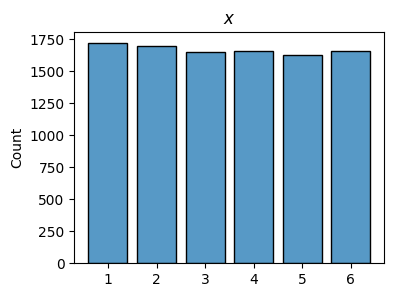
\includegraphics{notebooks/vector-spaces_files/figure-pdf/cell-5-output-1.png}

}

\end{figure}

What does adding two vectors do? Let \(\mathbf{v}=(v_x,v_y)\) and
\(\mathbf{w}=(w_x,w_y)\) be two vectors in the plane. Then their sum is
\(\mathbf{v}+\mathbf{w} = (v_x+w_x,v_y+w_y)\). I'll plot an example
below with \(\mathbf{v}=(1,1)\) and \(\mathbf{w}=(1,3)\). Their sum
should be

\[\mathbf{v}+\mathbf{w}=(1+1,1+3)=(2,4).\]

\begin{Shaded}
\begin{Highlighting}[]
\NormalTok{v }\OperatorTok{=}\NormalTok{ np.array([}\DecValTok{1}\NormalTok{, }\DecValTok{1}\NormalTok{])}
\NormalTok{w }\OperatorTok{=}\NormalTok{ np.array([}\DecValTok{1}\NormalTok{, }\DecValTok{3}\NormalTok{])}
\NormalTok{plot\_vectors([v, w, v }\OperatorTok{+}\NormalTok{ w], xlim}\OperatorTok{=}\NormalTok{(}\DecValTok{0}\NormalTok{, }\DecValTok{3}\NormalTok{), ylim}\OperatorTok{=}\NormalTok{(}\DecValTok{0}\NormalTok{, }\DecValTok{5}\NormalTok{), title}\OperatorTok{=}\SpecialStringTok{f\textquotesingle{}Adding Two Vectors\textquotesingle{}}\NormalTok{, ticks\_every}\OperatorTok{=}\DecValTok{1}\NormalTok{,}
\NormalTok{             labels}\OperatorTok{=}\NormalTok{[}\StringTok{\textquotesingle{}$\textbackslash{}mathbf}\SpecialCharTok{\{v\}}\StringTok{$\textquotesingle{}}\NormalTok{, }\StringTok{\textquotesingle{}$\textbackslash{}mathbf}\SpecialCharTok{\{w\}}\StringTok{$\textquotesingle{}}\NormalTok{, }\StringTok{\textquotesingle{}$\textbackslash{}mathbf}\SpecialCharTok{\{v\}}\StringTok{+\textbackslash{}mathbf}\SpecialCharTok{\{w\}}\StringTok{$\textquotesingle{}}\NormalTok{], }
\NormalTok{             colors}\OperatorTok{=}\NormalTok{[}\StringTok{\textquotesingle{}salmon\textquotesingle{}}\NormalTok{, }\StringTok{\textquotesingle{}steelblue\textquotesingle{}}\NormalTok{, }\StringTok{\textquotesingle{}black\textquotesingle{}}\NormalTok{])}
\end{Highlighting}
\end{Shaded}

\begin{figure}[H]

{\centering 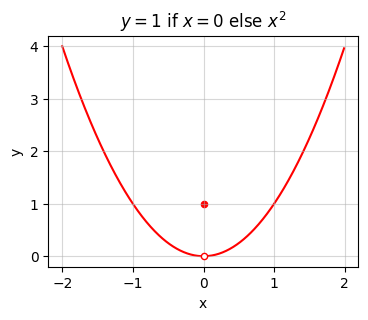
\includegraphics{notebooks/vector-spaces_files/figure-pdf/cell-6-output-1.png}

}

\end{figure}

It may not be obvious yet what vector addition is doing geometrically.
Let me plot it slightly differently. What I'll do is plot the vectors
``head to tail'' by taking the \emph{tail} of \(\mathbf{w}\) and placing
it at the \emph{head} of \(\mathbf{v}\). Then the head of this
translated \(\mathbf{w}\) vector points at the head of the sum
\(\mathbf{v}+\mathbf{w}\). We can do this ``head to tail'' stuff since
the base of a vector is irrelevant. We can place the arrow wherever we
want as long as we maintain its length and direction.

Informally speaking, to add two vectors, just stack them on top of each
other head to tail, and draw an arrow from the starting point to the
ending point. You can geometrically add arbitrarily many vectors this
way, not just two. Just keep stacking them.

\begin{Shaded}
\begin{Highlighting}[]
\NormalTok{plot\_vectors([v, w, v }\OperatorTok{+}\NormalTok{ w], xlim}\OperatorTok{=}\NormalTok{(}\DecValTok{0}\NormalTok{, }\DecValTok{3}\NormalTok{), ylim}\OperatorTok{=}\NormalTok{(}\DecValTok{0}\NormalTok{, }\DecValTok{5}\NormalTok{), title}\OperatorTok{=}\SpecialStringTok{f\textquotesingle{}Adding Two Vectors (Head to Tail)\textquotesingle{}}\NormalTok{,}
\NormalTok{             colors}\OperatorTok{=}\NormalTok{[}\StringTok{\textquotesingle{}salmon\textquotesingle{}}\NormalTok{, }\StringTok{\textquotesingle{}steelblue\textquotesingle{}}\NormalTok{, }\StringTok{\textquotesingle{}black\textquotesingle{}}\NormalTok{],}
\NormalTok{             tails}\OperatorTok{=}\NormalTok{[[}\DecValTok{0}\NormalTok{, }\DecValTok{0}\NormalTok{], [v[}\DecValTok{0}\NormalTok{], v[}\DecValTok{1}\NormalTok{]], [}\DecValTok{0}\NormalTok{, }\DecValTok{0}\NormalTok{]], text\_offsets}\OperatorTok{=}\NormalTok{[[}\OperatorTok{{-}}\FloatTok{0.5}\NormalTok{, }\OperatorTok{{-}}\FloatTok{0.85}\NormalTok{], [}\FloatTok{0.5}\NormalTok{, }\OperatorTok{{-}}\FloatTok{0.8}\NormalTok{], [}\OperatorTok{{-}}\FloatTok{1.4}\NormalTok{, }\OperatorTok{{-}}\FloatTok{1.6}\NormalTok{]],}
\NormalTok{             labels}\OperatorTok{=}\NormalTok{[}\StringTok{\textquotesingle{}$\textbackslash{}mathbf}\SpecialCharTok{\{v\}}\StringTok{$\textquotesingle{}}\NormalTok{, }\StringTok{\textquotesingle{}$\textbackslash{}mathbf}\SpecialCharTok{\{w\}}\StringTok{$\textquotesingle{}}\NormalTok{, }\StringTok{\textquotesingle{}$\textbackslash{}mathbf}\SpecialCharTok{\{v\}}\StringTok{+\textbackslash{}mathbf}\SpecialCharTok{\{w\}}\StringTok{$\textquotesingle{}}\NormalTok{],}
\NormalTok{             zorders }\OperatorTok{=}\NormalTok{ [}\DecValTok{0}\NormalTok{, }\DecValTok{1}\NormalTok{, }\DecValTok{2}\NormalTok{], ticks\_every}\OperatorTok{=}\DecValTok{1}\NormalTok{)}
\end{Highlighting}
\end{Shaded}

\begin{figure}[H]

{\centering \includegraphics{notebooks/vector-spaces_files/figure-pdf/cell-7-output-1.png}

}

\end{figure}

The norm satisfies what's known as the \textbf{triangle inequality}: If
\(\mathbf{v}\) and \(\mathbf{w}\) are two vectors, then the length of
their sum is less than the sum of their individual lengths, i.e.

\[||\mathbf{v}+\mathbf{w}|| \leq ||\mathbf{v}|| + ||\mathbf{w}||.\]

You can see this by staring at the plot above. The added lengths of
\(\mathbf{v}\) and \(\mathbf{w}\) is larger than the length of their sum
\(\mathbf{v}+\mathbf{w}\). In fact, the only time the lengths will be
equal is if \(\mathbf{v}\) and \(\mathbf{w}\) are parallel to each
other.

What about subtracting two vectors? By combining the rules for scalar
multiplication and vector addition, you can convince yourself that the
difference of two vectors is also element-wise,

\[\mathbf{v}-\mathbf{w} = (v_x-w_x,v_y-w_y).\]

To visualize what subtracting two vectors looks like, notice we can
write subtraction as a sum like this,
\(\mathbf{w} + (\mathbf{v}-\mathbf{w}) = \mathbf{v}\). Now use the same
trick for adding vectors, only this time placing
\((\mathbf{v}-\mathbf{w})\) at the head of \(\mathbf{w}\), and noticing
that it points to the sum of the two, which is \(\mathbf{v}\).

An easy way to remember what subtracting two vectors looks like is to
connect the two vectors you're subtracting with a line segment, and
place the head on the first vector. This trick will never fail you.

\begin{Shaded}
\begin{Highlighting}[]
\NormalTok{v }\OperatorTok{=}\NormalTok{ np.array([}\DecValTok{1}\NormalTok{, }\DecValTok{1}\NormalTok{])}
\NormalTok{w }\OperatorTok{=}\NormalTok{ np.array([}\DecValTok{1}\NormalTok{, }\DecValTok{3}\NormalTok{])}
\NormalTok{plot\_vectors([v, w, v }\OperatorTok{{-}}\NormalTok{ w], xlim}\OperatorTok{=}\NormalTok{(}\OperatorTok{{-}}\FloatTok{0.5}\NormalTok{, }\FloatTok{1.5}\NormalTok{), ylim}\OperatorTok{=}\NormalTok{(}\OperatorTok{{-}}\FloatTok{0.5}\NormalTok{, }\FloatTok{3.5}\NormalTok{), title}\OperatorTok{=}\SpecialStringTok{f\textquotesingle{}Subtracting Two Vectors\textquotesingle{}}\NormalTok{, headwidth}\OperatorTok{=}\DecValTok{4}\NormalTok{,}
\NormalTok{             ticks\_every}\OperatorTok{=}\DecValTok{1}\NormalTok{, colors}\OperatorTok{=}\NormalTok{[}\StringTok{\textquotesingle{}salmon\textquotesingle{}}\NormalTok{, }\StringTok{\textquotesingle{}steelblue\textquotesingle{}}\NormalTok{, }\StringTok{\textquotesingle{}black\textquotesingle{}}\NormalTok{],}
\NormalTok{             tails}\OperatorTok{=}\NormalTok{[[}\DecValTok{0}\NormalTok{, }\DecValTok{0}\NormalTok{], [}\DecValTok{0}\NormalTok{, }\DecValTok{0}\NormalTok{], [w[}\DecValTok{0}\NormalTok{], w[}\DecValTok{1}\NormalTok{]]], text\_offsets}\OperatorTok{=}\NormalTok{[[}\OperatorTok{{-}}\FloatTok{0.5}\NormalTok{, }\OperatorTok{{-}}\FloatTok{0.8}\NormalTok{], [}\OperatorTok{{-}}\FloatTok{0.5}\NormalTok{, }\OperatorTok{{-}}\DecValTok{1}\NormalTok{], [}\FloatTok{1.05}\NormalTok{, }\FloatTok{3.8}\NormalTok{]],}
\NormalTok{             labels}\OperatorTok{=}\NormalTok{[}\StringTok{\textquotesingle{}$\textbackslash{}mathbf}\SpecialCharTok{\{v\}}\StringTok{$\textquotesingle{}}\NormalTok{, }\StringTok{\textquotesingle{}$\textbackslash{}mathbf}\SpecialCharTok{\{w\}}\StringTok{$\textquotesingle{}}\NormalTok{, }\StringTok{\textquotesingle{}$\textbackslash{}mathbf}\SpecialCharTok{\{v\}}\StringTok{{-}\textbackslash{}mathbf}\SpecialCharTok{\{w\}}\StringTok{$\textquotesingle{}}\NormalTok{])}
\end{Highlighting}
\end{Shaded}

\begin{figure}[H]

{\centering \includegraphics{notebooks/vector-spaces_files/figure-pdf/cell-8-output-1.png}

}

\end{figure}

\hypertarget{the-dot-product}{%
\subsection{The Dot Product}\label{the-dot-product}}

It turns out we can understand both the lengths and angles of vectors in
terms of a single operation called the \textbf{dot product}, also called
the inner or scalar product. The dot product is a kind of multiplication
between two vectors that returns a scalar. If \(\mathbf{v}=(v_x,v_y)\)
and \(\mathbf{w}=(w_x,w_y)\) are two vectors in the plane, their dot
product is defined as

\[\mathbf{v} \cdot \mathbf{w} = v_x w_x + v_y w_y.\]

That is, the dot product is just the sum of the element-wise products of
the two vectors.

In terms of vectorized numpy code, the dot product is just the operation
\texttt{np.sum(v\ *\ w)}. Numpy also has a convenience function
\texttt{np.dot(v,\ w)} that calculates it directly. Here's the
calculation of the dot product between the two vectors
\(\mathbf{v}=(5,-1)\) and \(\mathbf{w}=(2,4)\). The answer should be

\[\mathbf{v} \cdot \mathbf{w} = 5 \cdot 2 + (-1) \cdot 4 = 10 - 4 = 6.\]

\begin{Shaded}
\begin{Highlighting}[]
\NormalTok{v }\OperatorTok{=}\NormalTok{ np.array([}\DecValTok{5}\NormalTok{, }\OperatorTok{{-}}\DecValTok{1}\NormalTok{])}
\NormalTok{w }\OperatorTok{=}\NormalTok{ np.array([}\DecValTok{2}\NormalTok{, }\DecValTok{4}\NormalTok{])}
\BuiltInTok{print}\NormalTok{(}\SpecialStringTok{f\textquotesingle{}v . w = }\SpecialCharTok{\{}\NormalTok{np}\SpecialCharTok{.}\NormalTok{dot(v, w)}\SpecialCharTok{\}}\SpecialStringTok{\textquotesingle{}}\NormalTok{)}
\NormalTok{np.}\BuiltInTok{sum}\NormalTok{(v }\OperatorTok{*}\NormalTok{ w) }\OperatorTok{==}\NormalTok{ np.dot(v, w)}
\end{Highlighting}
\end{Shaded}

\begin{verbatim}
v . w = 6
\end{verbatim}

\begin{verbatim}
True
\end{verbatim}

\textbf{Algorithm Analysis:} Evaluating the dot product uses \(2n-1\) or
\(O(n)\) total FLOPS, since for a vector of size \(n\) there are \(n\)
multiplications and \(n-1\) additions.

Here are some fairly trivial properties the dot product satisfies. These
follow straight from the definition.

\begin{itemize}
\tightlist
\item
  The dot product of a vector with itself is nonnegative:
  \(\mathbf{v} \cdot \mathbf{v} \geq 0\).
\item
  It commutes:
  \(\mathbf{v} \cdot \mathbf{w} = \mathbf{w} \cdot \mathbf{v}\).
\item
  It distributes over scalar multiplication:
  \(c\mathbf{v} \cdot \mathbf{w} = \mathbf{v} \cdot c\mathbf{w} = c(\mathbf{v} \cdot \mathbf{w})\).
\item
  It distributes over vector addition:
  \((\mathbf{u} + \mathbf{v}) \cdot \mathbf{w} = \mathbf{u} \cdot \mathbf{w} + \mathbf{v} \cdot \mathbf{w}\)
  and
  \(\mathbf{v} \cdot (\mathbf{u}+\mathbf{w}) = \mathbf{v} \cdot \mathbf{u} + \mathbf{v} \cdot \mathbf{w}\).
\end{itemize}

\textbf{Notation}: The dot product is often written in several different
ways in different fields. Another notation arises by thinking of the dot
product as the matrix multiplication of a \emph{row vector}
\(\mathbf{v}^\top = \begin{pmatrix}v_x & v_y \end{pmatrix}\) with a
\emph{column vector}
\(\mathbf{w} = \begin{pmatrix} w_x \\ w_y \end{pmatrix}\). In that case,

\[
\mathbf{v}^\top \mathbf{w} = 
\begin{pmatrix} v_x & v_y \end{pmatrix}
\begin{pmatrix} w_x \\ w_y \end{pmatrix}
= v_x w_x + v_y w_y = \mathbf{v} \cdot \mathbf{w}.
\]

This is the most commonly used notation for the dot product in machine
learning. I'll use it more frequently after this lesson.

We can write the norm or length of a vector in terms of the dot product.
Observe that by dotting \(\mathbf{v}\) with itself, I get

\[\mathbf{v} \cdot \mathbf{v} = v_x^2 + v_y^2 = ||\mathbf{v}||^2.\]

Taking the square root of both sides, you can see that the norm or
length of a vector is just the square root of its dot product with
itself,

\[||\mathbf{v}|| = \sqrt{\mathbf{v} \cdot \mathbf{v}}.\]

We can also talk about the \textbf{distance} between any two vectors
\(\mathbf{v}\) and \(\mathbf{w}\). Denote the distance between these two
vectors as \(d(\mathbf{v}, \mathbf{w})\). Since the difference vector is
\(\mathbf{v} - \mathbf{w}\), the distance between the two vectors is
evidently just the length of the difference vector,

\[d(\mathbf{v}, \mathbf{w}) = ||\mathbf{v} - \mathbf{w}|| = \sqrt{(\mathbf{v} - \mathbf{w}) \cdot (\mathbf{v} - \mathbf{w})} = \sqrt{(v_x-w_x)^2 - (v_y-w_y)^2}.\]

For example, the distance between the two vectors \(\mathbf{v}=(1,1)\)
and \(\mathbf{w}=(1, 0)\) is

\[d(\mathbf{v}, \mathbf{w}) = ||\mathbf{v} - \mathbf{w}|| = \sqrt{(1-1)^2 + (1-0)^2} = 1.\]

If a vector \(\mathbf{e}\) has norm \(||\mathbf{e}||=1\) it's called a
\textbf{unit vector}. We can convert any non-zero vector \(\mathbf{v}\)
into a unit vector by dividing by its norm, which is called
\textbf{normalizing} \(\mathbf{v}\). The unit vector gotten from
normalizing \(\mathbf{v}\) I'll call \(\mathbf{e_v}\). It's given by

\[\mathbf{e_v} = \frac{\mathbf{v}}{||\mathbf{v}||}.\]

For example, if \(\mathbf{v}=(1,1)\), its norm is
\(||\mathbf{v}||=\sqrt{2}\), so if we wanted to normalize it into a new
unit vector \(\mathbf{e_v}\), we'd have

\[\mathbf{e_v} = \frac{\mathbf{v}}{||\mathbf{v}||} = \frac{\mathbf{v}}{\sqrt{2}} = \frac{1}{\sqrt{2}}(1,1) \approx (0.707, 0.707).\]

Unit vectors will always point in the same direction as the vector used
to normalize them. The only difference is they'll have length one. In
the plane, unit vectors will always lie along the unit circle. Here's a
plot of this idea using the previous example.

\begin{Shaded}
\begin{Highlighting}[]
\NormalTok{v }\OperatorTok{=}\NormalTok{ np.array([}\DecValTok{1}\NormalTok{, }\DecValTok{2}\NormalTok{])}
\NormalTok{ev }\OperatorTok{=}\NormalTok{ v }\OperatorTok{/}\NormalTok{ np.sqrt(}\DecValTok{2}\NormalTok{)}
\NormalTok{plot\_vectors([v, ev], title}\OperatorTok{=}\StringTok{\textquotesingle{}$\textbackslash{}mathbf}\SpecialCharTok{\{e\}}\StringTok{\_v = ||\textbackslash{}mathbf}\SpecialCharTok{\{v\}}\StringTok{||\^{}\{{-}1\} \textbackslash{}mathbf}\SpecialCharTok{\{v\}}\StringTok{$\textquotesingle{}}\NormalTok{, ticks\_every}\OperatorTok{=}\FloatTok{0.5}\NormalTok{, zorders}\OperatorTok{=}\NormalTok{[}\DecValTok{0}\NormalTok{, }\DecValTok{1}\NormalTok{],}
\NormalTok{             text\_offsets}\OperatorTok{=}\NormalTok{[[}\FloatTok{0.01}\NormalTok{, }\FloatTok{0.05}\NormalTok{], [}\OperatorTok{{-}}\FloatTok{0.2}\NormalTok{, }\FloatTok{0.2}\NormalTok{]], colors}\OperatorTok{=}\NormalTok{[}\StringTok{\textquotesingle{}steelblue\textquotesingle{}}\NormalTok{, }\StringTok{\textquotesingle{}red\textquotesingle{}}\NormalTok{],}
\NormalTok{             labels}\OperatorTok{=}\NormalTok{[}\StringTok{\textquotesingle{}$\textbackslash{}mathbf}\SpecialCharTok{\{v\}}\StringTok{$\textquotesingle{}}\NormalTok{, }\StringTok{\textquotesingle{}$\textbackslash{}mathbf}\SpecialCharTok{\{e\}}\StringTok{\_v$\textquotesingle{}}\NormalTok{], headwidth}\OperatorTok{=}\DecValTok{6}\NormalTok{)}
\end{Highlighting}
\end{Shaded}

\begin{figure}[H]

{\centering \includegraphics{notebooks/vector-spaces_files/figure-pdf/cell-10-output-1.png}

}

\end{figure}

\hypertarget{projections}{%
\subsection{Projections}\label{projections}}

Let \(\mathbf{e}_x=(1,0)\). It's the unit vector pointing along the
positive x-axis. Notice the dot product between
\(\mathbf{v}=(v_x, v_y)\) and \(\mathbf{e}_x\) is just

\[\mathbf{v} \cdot \mathbf{e}_x = v_x \cdot 1 + v_y \cdot 0 = v_x.\]

Evidently the dot product \(\mathbf{v} \cdot \mathbf{e}_x\) ``picks''
out the x-component of \(\mathbf{v}\), namely \(v_x\). The vector
\(v_x \mathbf{e}_x = (v_x,0)\) gotten by rescaling \(\mathbf{e}_x\) by
\(v_x\) is called the \textbf{projection} of \(\mathbf{v}\) onto the
x-axis. It's the vector you'd get by dropping \(\mathbf{v}\)
perpendicular to the x-axis.

Similarly, if \(\mathbf{e}_y = (0,1)\) is the unit vector along the
positive y-axis, we can ``pick out'' the y-component of \(\mathbf{v}\)
by taking the dot product of \(\mathbf{v}\) with \(\mathbf{e}_y\),
i.e.~\(v_y = \mathbf{v} \cdot \mathbf{e}_y\). The vector
\(v_y\mathbf{e}_y\) is the projection of \(\mathbf{v}\) onto the y-axis.

Evidently, then, \(\mathbf{v}\) is just the sum of projections of
\(\mathbf{v}\) onto all of the axes,

\[\mathbf{v} = v_x \mathbf{e_x} + v_y \mathbf{e_y}.\]

This is yet another way to express a vector in terms of its components.
Just project down onto the axes and sum up the linear combination.

Here's what this looks like when \(\mathbf{v}=(0.5,1)\). In this
example, the projection onto the x-axis is just
\(v_x \mathbf{e}_x=(0.5, 0)\), and the projection onto the y-axis is
just \(v_y \mathbf{e_y}=(0,1)\). Using these projections, we can write
\(\mathbf{v}=(0.5,1)\) as
\(\mathbf{v} = 0.5 \mathbf{e}_x + \mathbf{e}_y\).

\begin{Shaded}
\begin{Highlighting}[]
\NormalTok{v }\OperatorTok{=}\NormalTok{ np.array([}\DecValTok{1}\NormalTok{, }\DecValTok{2}\NormalTok{])}
\NormalTok{ex }\OperatorTok{=}\NormalTok{ np.array([}\DecValTok{1}\NormalTok{, }\DecValTok{0}\NormalTok{])}
\NormalTok{ey }\OperatorTok{=}\NormalTok{ np.array([}\DecValTok{0}\NormalTok{, }\DecValTok{1}\NormalTok{])}
\NormalTok{plot\_vectors([v, v[}\DecValTok{0}\NormalTok{] }\OperatorTok{*}\NormalTok{ ex, v[}\DecValTok{1}\NormalTok{] }\OperatorTok{*}\NormalTok{ ey], title}\OperatorTok{=}\StringTok{\textquotesingle{}Projections Of $\textbackslash{}mathbf}\SpecialCharTok{\{v\}}\StringTok{$\textquotesingle{}}\NormalTok{, ticks\_every}\OperatorTok{=}\FloatTok{0.5}\NormalTok{,}
\NormalTok{             text\_offsets}\OperatorTok{=}\NormalTok{[[}\FloatTok{0.02}\NormalTok{, }\FloatTok{0.1}\NormalTok{], [}\OperatorTok{{-}}\FloatTok{0.1}\NormalTok{, }\FloatTok{0.2}\NormalTok{], [}\FloatTok{0.05}\NormalTok{, }\FloatTok{0.05}\NormalTok{]], colors}\OperatorTok{=}\NormalTok{[}\StringTok{\textquotesingle{}red\textquotesingle{}}\NormalTok{, }\StringTok{\textquotesingle{}steelblue\textquotesingle{}}\NormalTok{, }\StringTok{\textquotesingle{}steelblue\textquotesingle{}}\NormalTok{],}
\NormalTok{             labels}\OperatorTok{=}\NormalTok{[}\StringTok{\textquotesingle{}$\textbackslash{}mathbf}\SpecialCharTok{\{v\}}\StringTok{$\textquotesingle{}}\NormalTok{, }\StringTok{\textquotesingle{}$v\_x \textbackslash{}mathbf}\SpecialCharTok{\{e\}}\StringTok{\_x$\textquotesingle{}}\NormalTok{, }\StringTok{\textquotesingle{}$v\_y \textbackslash{}mathbf}\SpecialCharTok{\{e\}}\StringTok{\_y$\textquotesingle{}}\NormalTok{], headwidth}\OperatorTok{=}\DecValTok{4}\NormalTok{,}
\NormalTok{             xlim}\OperatorTok{=}\NormalTok{(}\OperatorTok{{-}}\FloatTok{0.5}\NormalTok{, }\FloatTok{2.5}\NormalTok{), ylim}\OperatorTok{=}\NormalTok{(}\OperatorTok{{-}}\FloatTok{0.5}\NormalTok{, }\FloatTok{2.5}\NormalTok{))}
\end{Highlighting}
\end{Shaded}

\begin{figure}[H]

{\centering \includegraphics{notebooks/vector-spaces_files/figure-pdf/cell-11-output-1.png}

}

\end{figure}

\hypertarget{linear-independence}{%
\subsection{Linear Independence}\label{linear-independence}}

I just showed we can decompose any vector
\(\mathbf{v} \in \mathbb{R}^2\) into its projections
\(\mathbf{v} = v_x \mathbf{e}_x + v_y \mathbf{e}_y\). The fact we can do
this is because the unit vectors \(\mathbf{e}_x\) and \(\mathbf{e}_y\)
are special, for a few reasons.

The first reason these vectors are special is that they don't lie along
the same line in the plane. Said differently, we can't write one vector
as a scalar multiple of the other, \(\mathbf{e}_x \neq c \mathbf{e}_y\)
for any scalar \(c\). Vectors with this property are called
\emph{linearly independent}.

More generally, a set of \(k\) vectors
\(\mathbf{v}_0, \mathbf{v}_1, \cdots, \mathbf{v}_{k-1}\) is called
\textbf{linearly independent} if no one vector \(\mathbf{v}_j\) in the
set can be written as a linear combination of the rest, i.e.~for
\emph{any} choice of scalars \(c_i\),

\[\mathbf{v}_j \neq \sum_{i \neq j} c_i \mathbf{v}_i.\]

A set of vectors that isn't linearly independent is called
\textbf{linearly dependent}. In a linearly dependent set, you can always
express at least one vector as a linear combination of the rest, for
example by finding a choice of scalars \(c_i\), you could write
\(\mathbf{v}_0\) as

\[\mathbf{v}_0 = \sum_{i=1}^{k-1} c_i \mathbf{v}_i = c_1 \mathbf{v}_1 + c_2 \mathbf{v}_2 + \cdots + c_{k-1} \mathbf{v}_{k-1}.\]

Linearly dependent sets of vectors are redundant in a sense. We have
more than we need. We can always keep dropping vectors from the set
until the ones remaining are linearly independent.

The vector space spanned by all linear combinations of a set of vectors
is called the \textbf{span} of that set. The span of a single vector
will always be a \emph{line}, since a linear combination of any one
vector is just the scalar multiples of that vector. The span of any
\emph{two} linearly independent vectors will always be a \emph{plane}.
The span of \(k\) linearly independent vectors will form a
\(k\)-dimensional \emph{hyperplane}.

As a simple example, consider the following set of vectors in the plane,

\begin{align*}
\mathbf{v}_0 &= (1, 0), \\
\mathbf{v}_1 &= (0, 1), \\
\mathbf{v}_2 &= (1, 1).
\end{align*}

If you stare at these for a second, you'll see that
\(\mathbf{v}_2 = \mathbf{v}_0 + \mathbf{v}_1\), so this set can't be
linearly independent. The third vector is redundant. Any two vectors in
this set span the exact same plane \(\mathbb{R}^2\). In fact, you'll
never have more than 2 linearly independent vectors of size 2. Why?

\begin{Shaded}
\begin{Highlighting}[]
\NormalTok{v0 }\OperatorTok{=}\NormalTok{ np.array([}\DecValTok{1}\NormalTok{, }\DecValTok{0}\NormalTok{])}
\NormalTok{v1 }\OperatorTok{=}\NormalTok{ np.array([}\DecValTok{0}\NormalTok{, }\DecValTok{1}\NormalTok{])}
\NormalTok{v2 }\OperatorTok{=}\NormalTok{ np.array([}\DecValTok{1}\NormalTok{, }\DecValTok{1}\NormalTok{])}
\NormalTok{plot\_vectors(}
\NormalTok{    [v2, v0, v1], colors}\OperatorTok{=}\NormalTok{[}\StringTok{\textquotesingle{}salmon\textquotesingle{}}\NormalTok{, }\StringTok{\textquotesingle{}steelblue\textquotesingle{}}\NormalTok{, }\StringTok{\textquotesingle{}limegreen\textquotesingle{}}\NormalTok{], xlim}\OperatorTok{=}\NormalTok{(}\OperatorTok{{-}}\FloatTok{0.5}\NormalTok{, }\FloatTok{1.5}\NormalTok{), ylim}\OperatorTok{=}\NormalTok{(}\OperatorTok{{-}}\FloatTok{0.5}\NormalTok{, }\FloatTok{1.5}\NormalTok{),}
\NormalTok{    ticks\_every}\OperatorTok{=}\FloatTok{0.5}\NormalTok{, zorders}\OperatorTok{=}\NormalTok{[}\DecValTok{0}\NormalTok{, }\DecValTok{1}\NormalTok{, }\DecValTok{2}\NormalTok{, }\DecValTok{3}\NormalTok{], headwidth}\OperatorTok{=}\DecValTok{5}\NormalTok{, text\_offsets}\OperatorTok{=}\NormalTok{[[}\FloatTok{0.03}\NormalTok{, }\FloatTok{0.05}\NormalTok{], [}\FloatTok{0.03}\NormalTok{,}\FloatTok{0.05}\NormalTok{], [}\FloatTok{0.03}\NormalTok{,}\FloatTok{0.05}\NormalTok{]],}
\NormalTok{    title}\OperatorTok{=}\StringTok{\textquotesingle{}$\textbackslash{}mathbf}\SpecialCharTok{\{v\}}\StringTok{\_0$, $\textbackslash{}mathbf}\SpecialCharTok{\{v\}}\StringTok{\_1$, $\textbackslash{}mathbf}\SpecialCharTok{\{v\}}\StringTok{\_2=\textbackslash{}mathbf}\SpecialCharTok{\{v\}}\StringTok{\_0+\textbackslash{}mathbf}\SpecialCharTok{\{v\}}\StringTok{\_1$\textquotesingle{}}\NormalTok{, }
\NormalTok{    labels}\OperatorTok{=}\NormalTok{[}\StringTok{\textquotesingle{}$\textbackslash{}mathbf}\SpecialCharTok{\{v\}}\StringTok{\_2$\textquotesingle{}}\NormalTok{, }\StringTok{\textquotesingle{}$\textbackslash{}mathbf}\SpecialCharTok{\{v\}}\StringTok{\_0$\textquotesingle{}}\NormalTok{, }\StringTok{\textquotesingle{}$\textbackslash{}mathbf}\SpecialCharTok{\{v\}}\StringTok{\_1$\textquotesingle{}}\NormalTok{])}
\end{Highlighting}
\end{Shaded}

\begin{figure}[H]

{\centering \includegraphics{notebooks/vector-spaces_files/figure-pdf/cell-12-output-1.png}

}

\end{figure}

For vectors in \(\mathbb{R}^2\), there are only two possibilities, they
either lie on the same line, or they span the whole plane. This follows
from the fact that any vector \(\mathbf{v}\) can be decomposed as
\(\mathbf{v} = v_x \mathbf{e}_x + v_y \mathbf{e}_y\). An implication of
this fact is that a set of vectors in \(\mathbb{R}^2\) can only be
linearly independent if it contains only one or two vectors. If it
contains a third vector, that vector \emph{must} be a linear combination
of the other two. The maximum number of linearly independent vectors in
a set is the \textbf{dimension} of the vector space. Since
\(\mathbb{R}^2\) is 2-dimensional, it can only sustain 2 linearly
independent vectors at a time.

\hypertarget{basis-vectors}{%
\subsection{Basis Vectors}\label{basis-vectors}}

In \(\mathbb{R}^2\), if we can find any two vectors \(\mathbf{a}\) and
\(\mathbf{b}\) that are linearly independent, then we can write any
other vector \(\mathbf{v}\) as a linear combination of those two
vectors,

\[\mathbf{v} = v_a \mathbf{a} + v_b \mathbf{b}.\]

The set \(\{\mathbf{a}, \mathbf{b}\}\) is called a \emph{basis}. We can
use vectors in this set as a ``basis'' to write any other vector.

More generally, a set of \(k\) vectors
\(\mathbf{v}_0, \mathbf{v}_1, \cdots, \mathbf{v}_{k-1}\) form a
\textbf{basis} for a vector space if the following two conditions hold,

\begin{enumerate}
\def\labelenumi{\arabic{enumi}.}
\tightlist
\item
  The vectors are all linearly independent,
\item
  The vectors span the full vector space.
\end{enumerate}

Another way of saying the same thing is that a basis is a set of exactly
\(n\) linearly independent vectors, where \(n\) is the dimension of the
vector space. A basis contains the minimal number of vectors needed to
span the vector space.

The special vectors \(\mathbf{e}_x\) and \(\mathbf{e}_y\) form a basis
for \(\mathbb{R}^2\), since we can write any other vector as a linear
combination of those two. Not only are these two vectors a basis,
however. They satisfy two other useful properties,

\begin{enumerate}
\def\labelenumi{\arabic{enumi}.}
\tightlist
\item
  They're both unit vectors,
  \(||\mathbf{e}_x|| = ||\mathbf{e}_y|| = 1\).
\item
  They're \textbf{orthogonal} to each other, that is,
  \(\mathbf{e}_x \cdot \mathbf{e}_y = 0\).
\end{enumerate}

A basis satisfying these two properties is called an \textbf{orthonormal
basis}. An orthonormal basis is special in that it allows us to pick out
the components of a vector directly by just taking dot products with the
basis vectors. It's only true in an orthonormal basis that we can write
the components of a vector \(\mathbf{v}\) as,

\begin{align*}
v_x &= \mathbf{v} \cdot \mathbf{e}_x, \\
v_y &= \mathbf{v} \cdot \mathbf{e}_y.
\end{align*}

The set \(\{\mathbf{e}_x, \mathbf{e}_y\}\) is only one example of an
orthonormal basis for \(\mathbb{R}^2\). It's called the \textbf{standard
basis}, since it's the basis whose vectors point along the usual
positive x and y axes.

Expressing any vector in terms of its basis is just projecting the
vector down onto each of the basis axes. Let's do a quick example. Let
\(\mathbf{v}=(1.25,2)\) be a vector. Decomposed into the standard basis
we just get

\[\mathbf{v} = 1.25 \mathbf{e}_x + 2 \mathbf{e}_y.\]

Graphically this just looks as follows. We've already seen a plot like
this, except this time I'm including the basis vectors \(\mathbf{e}_x\)
and \(\mathbf{e}_y\) explicitly. Notice that the two basis vectors form
a \(90^\circ\) angle, i.e.~they're perpendicular. I'll show in a moment
that this is implied by the fact that
\(\mathbf{e}_x \cdot \mathbf{e}_y = 0\).

\begin{Shaded}
\begin{Highlighting}[]
\NormalTok{v }\OperatorTok{=}\NormalTok{ np.array([}\FloatTok{1.25}\NormalTok{, }\DecValTok{2}\NormalTok{])}
\NormalTok{ex }\OperatorTok{=}\NormalTok{ np.array([}\DecValTok{1}\NormalTok{, }\DecValTok{0}\NormalTok{])}
\NormalTok{ey }\OperatorTok{=}\NormalTok{ np.array([}\DecValTok{0}\NormalTok{, }\DecValTok{1}\NormalTok{])}
\NormalTok{plot\_vectors(}
\NormalTok{    [v, v[}\DecValTok{0}\NormalTok{] }\OperatorTok{*}\NormalTok{ ex, v[}\DecValTok{1}\NormalTok{] }\OperatorTok{*}\NormalTok{ ey, ex, ey], colors}\OperatorTok{=}\NormalTok{[}\StringTok{\textquotesingle{}red\textquotesingle{}}\NormalTok{, }\StringTok{\textquotesingle{}steelblue\textquotesingle{}}\NormalTok{, }\StringTok{\textquotesingle{}steelblue\textquotesingle{}}\NormalTok{, }\StringTok{\textquotesingle{}black\textquotesingle{}}\NormalTok{, }\StringTok{\textquotesingle{}black\textquotesingle{}}\NormalTok{], }
\NormalTok{    ticks\_every}\OperatorTok{=}\DecValTok{1}\NormalTok{, zorders}\OperatorTok{=}\NormalTok{[}\DecValTok{0}\NormalTok{, }\DecValTok{1}\NormalTok{, }\DecValTok{2}\NormalTok{, }\DecValTok{3}\NormalTok{, }\DecValTok{4}\NormalTok{, }\DecValTok{5}\NormalTok{], headwidth}\OperatorTok{=}\DecValTok{5}\NormalTok{,}
\NormalTok{    text\_offsets}\OperatorTok{=}\NormalTok{[[}\DecValTok{0}\NormalTok{,}\DecValTok{0}\NormalTok{], [}\DecValTok{0}\NormalTok{,}\FloatTok{0.2}\NormalTok{], [}\FloatTok{0.05}\NormalTok{,}\DecValTok{0}\NormalTok{], [}\OperatorTok{{-}}\FloatTok{0.2}\NormalTok{,}\FloatTok{0.2}\NormalTok{], [}\FloatTok{0.05}\NormalTok{,}\DecValTok{0}\NormalTok{]],}
\NormalTok{    title}\OperatorTok{=}\StringTok{\textquotesingle{}$\textbackslash{}mathbf}\SpecialCharTok{\{v\}}\StringTok{=v\_x \textbackslash{}mathbf}\SpecialCharTok{\{e\}}\StringTok{\_x + v\_y \textbackslash{}mathbf}\SpecialCharTok{\{e\}}\StringTok{\_y$\textquotesingle{}}\NormalTok{, }
\NormalTok{    labels}\OperatorTok{=}\NormalTok{[}\StringTok{\textquotesingle{}$\textbackslash{}mathbf}\SpecialCharTok{\{v\}}\StringTok{$\textquotesingle{}}\NormalTok{, }\StringTok{\textquotesingle{}$v\_x \textbackslash{}mathbf}\SpecialCharTok{\{e\}}\StringTok{\_x$\textquotesingle{}}\NormalTok{, }\StringTok{\textquotesingle{}$v\_y \textbackslash{}mathbf}\SpecialCharTok{\{e\}}\StringTok{\_y$\textquotesingle{}}\NormalTok{, }\StringTok{\textquotesingle{}$\textbackslash{}mathbf}\SpecialCharTok{\{e\}}\StringTok{\_x$\textquotesingle{}}\NormalTok{, }\StringTok{\textquotesingle{}$\textbackslash{}mathbf}\SpecialCharTok{\{e\}}\StringTok{\_y$\textquotesingle{}}\NormalTok{])}
\end{Highlighting}
\end{Shaded}

\begin{figure}[H]

{\centering \includegraphics{notebooks/vector-spaces_files/figure-pdf/cell-13-output-1.png}

}

\end{figure}

Of course, I already said the standard basis isn't the \emph{only}
orthonormal basis for \(\mathbb{R}^2\) we could choose. Here's an
example of another one that would work equally well. Let
\(\mathbf{e}_a=\frac{1}{\sqrt{2}} (1,1)\) and
\(\mathbf{e}_b=\frac{1}{\sqrt{2}} (-1,1)\). Notice that both vectors
have unit length, and they're orthogonal since
\(\mathbf{e}_a \cdot \mathbf{e}_b = 0\). Thus, they form an orthonormal
basis for \(\mathbb{R}^2\). In this basis, \(\mathbf{v}=(1.25, 2)\)
would be written

\[\mathbf{v} = (\mathbf{v} \cdot \mathbf{e}_a) \mathbf{e}_a + (\mathbf{v} \cdot \mathbf{e}_b) \mathbf{e}_b \approx 2.298 \mathbf{e}_a + 0.530 \mathbf{e}_b.\]

This is a very different representation for \(\mathbf{v}\).
Nevertheless, the two basis vectors are still perpendicular to each
other. You can see a plot of this below.

There are infinitely many orthonormal bases for \(\mathbb{R}^2\). Just
take any two perpendicular vectors in the plane and normalize them to
unit length and they'll form a valid orthonormal basis.

\begin{Shaded}
\begin{Highlighting}[]
\NormalTok{v }\OperatorTok{=}\NormalTok{ np.array([}\FloatTok{1.25}\NormalTok{, }\DecValTok{2}\NormalTok{])}
\NormalTok{ea }\OperatorTok{=}\NormalTok{ np.array([}\DecValTok{1}\NormalTok{, }\DecValTok{1}\NormalTok{]) }\OperatorTok{/}\NormalTok{ np.sqrt(}\DecValTok{2}\NormalTok{)}
\NormalTok{eb }\OperatorTok{=}\NormalTok{ np.array([}\OperatorTok{{-}}\DecValTok{1}\NormalTok{, }\DecValTok{1}\NormalTok{]) }\OperatorTok{/}\NormalTok{ np.sqrt(}\DecValTok{2}\NormalTok{)}
\NormalTok{vectors }\OperatorTok{=}\NormalTok{ [v, np.dot(v, ea) }\OperatorTok{*}\NormalTok{ ea, np.dot(v, eb) }\OperatorTok{*}\NormalTok{ eb, ea, eb]}
\NormalTok{plot\_vectors(}
\NormalTok{    vectors, ticks\_every}\OperatorTok{=}\DecValTok{1}\NormalTok{, zorders}\OperatorTok{=}\NormalTok{[}\DecValTok{0}\NormalTok{, }\DecValTok{1}\NormalTok{, }\DecValTok{5}\NormalTok{, }\DecValTok{3}\NormalTok{, }\DecValTok{4}\NormalTok{, }\DecValTok{2}\NormalTok{], headwidth}\OperatorTok{=}\DecValTok{7}\NormalTok{,}
\NormalTok{    colors}\OperatorTok{=}\NormalTok{[}\StringTok{\textquotesingle{}red\textquotesingle{}}\NormalTok{, }\StringTok{\textquotesingle{}steelblue\textquotesingle{}}\NormalTok{, }\StringTok{\textquotesingle{}steelblue\textquotesingle{}}\NormalTok{, }\StringTok{\textquotesingle{}black\textquotesingle{}}\NormalTok{, }\StringTok{\textquotesingle{}black\textquotesingle{}}\NormalTok{],}
\NormalTok{    text\_offsets}\OperatorTok{=}\NormalTok{[[}\DecValTok{0}\NormalTok{, }\DecValTok{0}\NormalTok{], [}\FloatTok{0.03}\NormalTok{, }\DecValTok{0}\NormalTok{], [}\OperatorTok{{-}}\FloatTok{0.3}\NormalTok{, }\OperatorTok{{-}}\FloatTok{0.65}\NormalTok{], [}\OperatorTok{{-}}\FloatTok{0.1}\NormalTok{, }\OperatorTok{{-}}\FloatTok{0.48}\NormalTok{], [}\OperatorTok{{-}}\FloatTok{0.2}\NormalTok{, }\FloatTok{0.15}\NormalTok{]],}
\NormalTok{    title}\OperatorTok{=}\StringTok{\textquotesingle{}$\textbackslash{}mathbf}\SpecialCharTok{\{v\}}\StringTok{=v\_a \textbackslash{}mathbf}\SpecialCharTok{\{e\}}\StringTok{\_a + v\_b \textbackslash{}mathbf}\SpecialCharTok{\{e\}}\StringTok{\_b$\textquotesingle{}}\NormalTok{, }
\NormalTok{    labels}\OperatorTok{=}\NormalTok{[}\StringTok{\textquotesingle{}$\textbackslash{}mathbf}\SpecialCharTok{\{v\}}\StringTok{$\textquotesingle{}}\NormalTok{, }\StringTok{\textquotesingle{}$v\_a \textbackslash{}mathbf}\SpecialCharTok{\{e\}}\StringTok{\_a$\textquotesingle{}}\NormalTok{, }\StringTok{\textquotesingle{}$v\_b \textbackslash{}mathbf}\SpecialCharTok{\{e\}}\StringTok{\_b$\textquotesingle{}}\NormalTok{, }\StringTok{\textquotesingle{}$\textbackslash{}mathbf}\SpecialCharTok{\{e\}}\StringTok{\_a$\textquotesingle{}}\NormalTok{, }\StringTok{\textquotesingle{}$\textbackslash{}mathbf}\SpecialCharTok{\{e\}}\StringTok{\_b$\textquotesingle{}}\NormalTok{])}
\end{Highlighting}
\end{Shaded}

\begin{figure}[H]

{\centering \includegraphics{notebooks/vector-spaces_files/figure-pdf/cell-14-output-1.png}

}

\end{figure}

\hypertarget{cosine-similarity}{%
\subsection{Cosine Similarity}\label{cosine-similarity}}

Just like we can express the length of a vector using the dot product,
it turns out we can also express the \emph{angle} between any two
vectors in the plane using the dot product. If \(\theta\) is the angle
between two vectors \(\mathbf{v}\) and \(\mathbf{w}\), it turns out the
dot product is given by

\[\mathbf{v} \cdot \mathbf{w} = ||\mathbf{v}|| \cdot ||\mathbf{w}|| \cos \theta.\]

Note that both sides of this equation are scalars since the dot product
is a scalar and the product of norms is a scalar. If you're good at
trigonometry, you can convince yourself this formula must be true by
projecting \(\mathbf{v}\) onto \(\mathbf{w}\) similar to the way we did
projections onto the x and y axes before. The difference this time is
that the component of \(\mathbf{v}\) in the direction of \(\mathbf{w}\)
is not \(v_x\) or \(v_y\) anymore, but instead
\(||\mathbf{v}|| \cos \theta\).

You can see two special cases of this formula by looking at what happens
when the two vectors are \emph{parallel} or \emph{perpendicular}. If the
two vectors are parallel, then \(\theta = 0^\circ, 180^\circ\), so
\(\cos \theta = \pm 1\), so
\(\mathbf{v} \cdot \mathbf{w} = \pm ||\mathbf{v}|| \cdot ||\mathbf{w}||\).
More importantly, if the two vectors are perpendicular, then
\(\theta = 90^\circ, 270^\circ\), so \(\cos \theta = 0\), so
\(\mathbf{v} \cdot \mathbf{w} = 0\). That is, perpendicular vectors are
\emph{orthogonal}. They mean the same thing.

It's more common to express this formula with \(\cos \theta\) on one
side and the vector terms on the other so you can solve for the angle
(or more commonly just the cosine of the angle). In this case, we have
\[\cos \theta = \frac{\mathbf{v} \cdot \mathbf{w}}{||\mathbf{v}|| \cdot ||\mathbf{w}||}.\]

What matters more than anything is what this formula says and how to use
it. Suppose, for example, you want to find the angle between the two
vectors \(\mathbf{v} = (1,1)\) and \(\mathbf{w} = (0, -1)\). Then you'd
have

\begin{align*}
\mathbf{v} \cdot \mathbf{w} &= 1 \cdot 0 + 1 \cdot (-1) = -1, \\
||\mathbf{v}|| &= \sqrt{1^2 + 1^2} = \sqrt{2}, \\
||\mathbf{w}|| &= \sqrt{0^2 + (-1)^2} = 1.
\end{align*}

Plugging this into the cosine formula gives,

\[
\cos \theta = \frac{-1}{\sqrt{2}} \quad \Longrightarrow \quad \theta = \cos^{-1}\bigg(\frac{-1}{\sqrt{2}}\bigg) = 135^\circ.
\]

You can verify this is correct by plotting the two vectors and
confirming that they're about \(135^\circ\) from each other, which
corresponds to about 1.25 quarter turns around a circle. It's
interesting to note that the dot product will only be negative when the
angle between the two vectors is obtuse, i.e.~more than \(90^\circ\),
which is of course the case here.

\begin{Shaded}
\begin{Highlighting}[]
\NormalTok{v }\OperatorTok{=}\NormalTok{ np.array([}\DecValTok{1}\NormalTok{, }\DecValTok{1}\NormalTok{])}
\NormalTok{w }\OperatorTok{=}\NormalTok{ np.array([}\DecValTok{0}\NormalTok{, }\OperatorTok{{-}}\DecValTok{1}\NormalTok{])}
\NormalTok{plot\_vectors([v, w], title}\OperatorTok{=}\StringTok{\textquotesingle{}$\textbackslash{}mathbf}\SpecialCharTok{\{v\}}\StringTok{ \textbackslash{}cdot \textbackslash{}mathbf}\SpecialCharTok{\{w\}}\StringTok{ = ||\textbackslash{}mathbf}\SpecialCharTok{\{v\}}\StringTok{||||\textbackslash{}mathbf}\SpecialCharTok{\{w\}}\StringTok{|| \textbackslash{}cos }\CharTok{\textbackslash{}\textbackslash{}}\StringTok{theta$\textquotesingle{}}\NormalTok{, }
\NormalTok{             text\_offsets}\OperatorTok{=}\NormalTok{[[}\DecValTok{0}\NormalTok{, }\DecValTok{0}\NormalTok{], [}\FloatTok{0.1}\NormalTok{, }\DecValTok{0}\NormalTok{]], ticks\_every}\OperatorTok{=}\FloatTok{0.5}\NormalTok{, xlim}\OperatorTok{=}\NormalTok{(}\OperatorTok{{-}}\DecValTok{1}\NormalTok{, }\DecValTok{2}\NormalTok{), ylim}\OperatorTok{=}\NormalTok{(}\OperatorTok{{-}}\FloatTok{1.5}\NormalTok{, }\FloatTok{1.5}\NormalTok{),}
\NormalTok{             labels}\OperatorTok{=}\NormalTok{[}\StringTok{\textquotesingle{}$\textbackslash{}mathbf}\SpecialCharTok{\{v\}}\StringTok{$\textquotesingle{}}\NormalTok{, }\StringTok{\textquotesingle{}$\textbackslash{}mathbf}\SpecialCharTok{\{w\}}\StringTok{$\textquotesingle{}}\NormalTok{], colors}\OperatorTok{=}\NormalTok{[}\StringTok{\textquotesingle{}red\textquotesingle{}}\NormalTok{, }\StringTok{\textquotesingle{}steelblue\textquotesingle{}}\NormalTok{], headwidth}\OperatorTok{=}\DecValTok{7}\NormalTok{)}
\end{Highlighting}
\end{Shaded}

\begin{figure}[H]

{\centering \includegraphics{notebooks/vector-spaces_files/figure-pdf/cell-15-output-1.png}

}

\end{figure}

In machine learning, this formula for \(\cos \theta\) is called the
\textbf{cosine similarity}. The reason for this is that the dot product
itself is a measure of how similar two vectors are. To see why, consider
two special cases:

\begin{itemize}
\tightlist
\item
  The two vectors are parallel: This is as large as the dot product
  between two vectors can get in absolute value. The vectors are as
  similar as they can be in a sense. Up to a scalar multiple, they
  contain the same information.
\item
  The two vectors are perpendicular: This is as small as the dot product
  between two vectors can get in absolute value. The two vectors are as
  different as they can be in a sense. They share pretty much no
  information. Information about one vector tells you basically nothing
  about the other.
\end{itemize}

The cosine similarity is a function of two input vectors \(\mathbf{v}\)
and \(\mathbf{w}\). Since we don't actually care about the angle
\(\theta\) usually, we'll more often denote the cosine similarity using
a notation like \(\cos(\mathbf{v},\mathbf{w})\) to make it clear it's a
function of its two input vectors,

\[\cos(\mathbf{v},\mathbf{w}) = \frac{\mathbf{v} \cdot \mathbf{w}}{||\mathbf{v}|| \cdot ||\mathbf{w}||}.\]

Note the cosine similarity is just a normalized dot product, since
dividing by the norms forces
\(-1 \leq \cos(\mathbf{v},\mathbf{w}) \leq 1\). It thus captures the
same idea of similarity that the dot product does, but it's more useful
when the lengths of vectors get out of control. This is particularly
likely to happen in high dimensions, when \(n >> 2\). This is the
so-called ``curse of dimensionality''. We'll come back to this idea in
future lessons.

Here's a quick implementation of the cosine similarity function using
numpy. There's no built-in function to do it, but it's easy enough to
implement by making judicious use of the \texttt{np.dot} function. It
should give the same answer found above for \(\cos \theta\), which is
\(-\frac{1}{\sqrt{2}} \approx -0.707\).

\begin{Shaded}
\begin{Highlighting}[]
\KeywordTok{def}\NormalTok{ cosine\_similarity(v, w):}
    \ControlFlowTok{return}\NormalTok{ np.dot(v, w) }\OperatorTok{/}\NormalTok{ np.sqrt(np.dot(v, v) }\OperatorTok{*}\NormalTok{ np.dot(w, w))}

\BuiltInTok{print}\NormalTok{(}\SpecialStringTok{f\textquotesingle{}cos(v, w) = }\SpecialCharTok{\{}\NormalTok{cosine\_similarity(v, w)}\SpecialCharTok{\}}\SpecialStringTok{\textquotesingle{}}\NormalTok{)}
\end{Highlighting}
\end{Shaded}

\begin{verbatim}
cos(v, w) = -0.7071067811865475
\end{verbatim}

\textbf{Algorithm Analysis:} Like the dot product, this function uses
only \(O(n)\) FLOPS. There are three independent dot product operations
happening here, each adding \(O(n)\) FLOPS. Since the outputs of dot
products are scalars, the multiply and divide only add one FLOP each.
The square root isn't obvious, but you can assume it takes some constant
number of FLOPS as well. The total must therefore be \(O(n)\).

\hypertarget{other-norms}{%
\subsection{Other Norms}\label{other-norms}}

It turns out that the norm I defined above is only \emph{one} way to
measure the length of a vector. It's the most natural way to do so sense
it corresponds to your intuitive notions of length, which itself relates
to the Pythagorean Theorem. There are other ways to quantify vector
length as well that aren't as intuitive. Because they do sometimes show
up in machine learning I'll briefly mention a couple of these here.

The norm I've covered is called the \textbf{2-norm}. It's called this
because it involves squares and square roots. We can write it in the
form

\[||\mathbf{v}|| = ||\mathbf{v}||_2 = \big(v_x^2 + v_y^2 \big)^{1/2}.\]

It turns out we can replace the twos with any other positive number
\(p>1\) to get generalized norms, called \textbf{p-norms},

\[||\mathbf{v}||_p = \big(v_x^p + v_y^p \big)^{1/p}.\]

The p-norms cover a large class of norms, since any
\(1 \leq p \leq \infty\) can define a valid norm. The 2-norm, as you'd
guess, occurs when \(p=2\). A couple of other norms that show up in
machine learning are the \textbf{1-norm} when \(p=1\), and the
\textbf{infinity norm} when \(p=\infty\). For 2-dimensional vectors,
these norms are

\begin{align*}
||\mathbf{v}||_1 &= |v_x| + |v_y|, \\
||\mathbf{v}||_\infty &= \max\big(|v_x|, |v_y|\big).
\end{align*}

Here's an example. I'll calculate the \(p=1, 2, \infty\) norms for the
vector \(\mathbf{v}=(1,-2)\). We have,

\begin{align*}
||\mathbf{v}||_1 &= |1| + |-2| = 1 + 2 = 3, \\
||\mathbf{v}||_2 &= \sqrt{1^2 + (-2)^2} = \sqrt{1 + 4} = \sqrt{5} \approx 2.236, \\
||\mathbf{v}||_\infty &= \max\big(|1|, |-2|\big) = \max(1, 2) = 2.
\end{align*}

Notice that
\(||\mathbf{v}||_1 \geq ||\mathbf{v}||_2 \geq ||\mathbf{v}||_\infty\).
This is a general fact.

It's a little hard right now to describe why these norms are useful in
machine learning since we don't currently have the context. Just know
that these norms do come up sometimes. I'll go into more depth on the
uses of these different norms as we apply them. In practice though,
we'll probably work with the regular 2-norm maybe 90\% of the time.

In numpy, you can calculate any \(p\)-norm using the function
\texttt{np.linalg.norm(v,\ ord=p)}. Here's an example.

\begin{Shaded}
\begin{Highlighting}[]
\NormalTok{v }\OperatorTok{=}\NormalTok{ np.array([}\DecValTok{1}\NormalTok{, }\OperatorTok{{-}}\DecValTok{2}\NormalTok{])}
\BuiltInTok{print}\NormalTok{(}\SpecialStringTok{f\textquotesingle{}1{-}Norm of v: }\SpecialCharTok{\{}\NormalTok{np}\SpecialCharTok{.}\NormalTok{linalg}\SpecialCharTok{.}\NormalTok{norm(v, }\BuiltInTok{ord}\OperatorTok{=}\DecValTok{1}\NormalTok{)}\SpecialCharTok{\}}\SpecialStringTok{\textquotesingle{}}\NormalTok{)}
\BuiltInTok{print}\NormalTok{(}\SpecialStringTok{f\textquotesingle{}2{-}Norm of v: }\SpecialCharTok{\{}\NormalTok{np}\SpecialCharTok{.}\NormalTok{linalg}\SpecialCharTok{.}\NormalTok{norm(v, }\BuiltInTok{ord}\OperatorTok{=}\DecValTok{2}\NormalTok{)}\SpecialCharTok{\}}\SpecialStringTok{\textquotesingle{}}\NormalTok{)}
\BuiltInTok{print}\NormalTok{(}\SpecialStringTok{f\textquotesingle{}Infinity{-}Norm of v: }\SpecialCharTok{\{}\NormalTok{np}\SpecialCharTok{.}\NormalTok{linalg}\SpecialCharTok{.}\NormalTok{norm(v, }\BuiltInTok{ord}\OperatorTok{=}\NormalTok{np.inf)}\SpecialCharTok{\}}\SpecialStringTok{\textquotesingle{}}\NormalTok{)}
\end{Highlighting}
\end{Shaded}

\begin{verbatim}
1-Norm of v: 3.0
2-Norm of v: 2.23606797749979
Infinity-Norm of v: 2.0
\end{verbatim}

\hypertarget{linear-maps}{%
\section{Linear Maps}\label{linear-maps}}

So where do matrices fit into all this vector space stuff? It turns out
that matrices correspond to functions between vectors to vectors. These
are called \textbf{linear maps}. A linear map is a vector-valued
function from one vector space to another that preserves the properties
of vectors. In \(\mathbb{R}^2\), a linear map is a function between
vectors \(\mathbf{v}=(v_x,v_y)\) and \(\mathbf{w}=(w_x,w_y)\) of the
form

\[\mathbf{w} = (w_x, w_y) = (av_x + bv_y, cv_x + dv_y) = \mathbf{F}(\mathbf{v}).\]

That is, each component of the output vector \(\mathbf{w}\) is a linear
combination of the input vector \(\mathbf{v}\). Now, if you stare at
this function for a little bit, you should see that this kind of looks
like a \(2 \times 2\) system of linear equations,

\begin{alignat*}{3}
   av_x & {}+{} &  bv_y & {}={} & w_x \\
   cv_x & {}+{} &  dv_y & {}={} & w_y.
\end{alignat*}

This of course means the linear map is equivalent to a matrix-vector
equation. If we identify \(\mathbf{v}\) and \(\mathbf{w}\) with
\(2 \times 1\) column vectors, and define a \(\mathbf{A}\) by

\[
\mathbf{A} = 
\begin{pmatrix}
a & b \\
c & d
\end{pmatrix},
\]

then the linear map \(\mathbf{w} = \mathbf{F}(\mathbf{v})\) is
equivalent to the matrix-vector equation
\(\mathbf{w}=\mathbf{A}\mathbf{v}\), or

\[\mathbf{F}(\mathbf{v}) = \mathbf{A}\mathbf{v}.\]

In fact, \emph{every} linear map \(\mathbf{F}(\mathbf{v})\) can be
identified with some matrix equation \(\mathbf{A}\mathbf{v}\). Knowing
\(\mathbf{A}\) (in some basis) is equivalent to knowing the linear map
itself.

But why are linear maps important? The main reason is that they preserve
linear structure. Notice that I can define a line through any vector
\(\mathbf{v}\) by scaling it with some parameter \(t\). If I apply a
linear map to this line I'd get
\(\mathbf{F}(t\mathbf{v}) = t\mathbf{F}(\mathbf{v})\). Check it yourself
from the definition. Said differently, linear maps map lines to lines,
thus preserving the linear structure of the vector space. The new line
won't usually be the \emph{original} line. It may get rotated. But it's
still a line.

Let's try to visualize what a linear map does by defining a particular
\(2 \times 2\) matrix \(\mathbf{A}\) and seeing how it acts on inputs
\(\mathbf{v}\).

\begin{Shaded}
\begin{Highlighting}[]
\NormalTok{A }\OperatorTok{=}\NormalTok{ np.array([[}\DecValTok{1}\NormalTok{, }\OperatorTok{{-}}\FloatTok{0.1}\NormalTok{], [}\FloatTok{0.1}\NormalTok{, }\DecValTok{1}\NormalTok{]])}
\NormalTok{v }\OperatorTok{=}\NormalTok{ np.array([}\DecValTok{1}\NormalTok{, }\DecValTok{1}\NormalTok{]).reshape(}\OperatorTok{{-}}\DecValTok{1}\NormalTok{, }\DecValTok{1}\NormalTok{)}
\NormalTok{plot\_vectors([v.flatten(), (A }\OperatorTok{@}\NormalTok{ v).flatten()], colors}\OperatorTok{=}\NormalTok{[}\StringTok{\textquotesingle{}black\textquotesingle{}}\NormalTok{, }\StringTok{\textquotesingle{}red\textquotesingle{}}\NormalTok{],}
\NormalTok{             labels}\OperatorTok{=}\NormalTok{[}\StringTok{\textquotesingle{}$\textbackslash{}mathbf}\SpecialCharTok{\{\{}\StringTok{v}\SpecialCharTok{\}\}}\StringTok{$\textquotesingle{}}\NormalTok{, }\StringTok{\textquotesingle{}$\textbackslash{}mathbf}\SpecialCharTok{\{\{}\StringTok{A}\SpecialCharTok{\}\}}\StringTok{\textbackslash{}mathbf}\SpecialCharTok{\{\{}\StringTok{v}\SpecialCharTok{\}\}}\StringTok{$\textquotesingle{}}\NormalTok{], text\_offsets}\OperatorTok{=}\NormalTok{[[}\FloatTok{0.01}\NormalTok{, }\OperatorTok{{-}}\FloatTok{0.1}\NormalTok{], [}\OperatorTok{{-}}\FloatTok{0.1}\NormalTok{, }\FloatTok{0.05}\NormalTok{]],}
\NormalTok{             title}\OperatorTok{=}\StringTok{\textquotesingle{}Linear Map: $\textbackslash{}mathbf}\SpecialCharTok{\{\{}\StringTok{w}\SpecialCharTok{\}\}}\StringTok{ = \textbackslash{}mathbf}\SpecialCharTok{\{\{}\StringTok{A}\SpecialCharTok{\}\}}\StringTok{\textbackslash{}mathbf}\SpecialCharTok{\{\{}\StringTok{v}\SpecialCharTok{\}\}}\StringTok{$\textquotesingle{}}\NormalTok{,  xlim}\OperatorTok{=}\NormalTok{(}\DecValTok{0}\NormalTok{, }\FloatTok{1.5}\NormalTok{), ylim}\OperatorTok{=}\NormalTok{(}\DecValTok{0}\NormalTok{, }\FloatTok{1.5}\NormalTok{))}
\end{Highlighting}
\end{Shaded}

\begin{figure}[H]

{\centering \includegraphics{notebooks/vector-spaces_files/figure-pdf/cell-18-output-1.png}

}

\end{figure}

Why stop there? Let's apply the linear map a whole bunch of times
recursively and see what happens to the output vectors \(\mathbf{w}\).
I'll plot each of the \(k=63\) vectors in the following sequence,
\[\mathbf{v}, \ \mathbf{A}\mathbf{v}, \ \mathbf{A}^2\mathbf{v}, \ \cdots, \ \mathbf{A}^{63}\mathbf{v}.\]

Note each power \(\mathbf{A}^j\) here is a \emph{matrix power}, defined
by applying \emph{matrix multiplication} over and over \(k\) times. It's
\emph{not} the element-wise power.

For the particular values in this plot I'll choose
\(\mathbf{v}=\begin{pmatrix} 1 \\ 1 \end{pmatrix}\) and
\(\mathbf{A}=\begin{pmatrix} 1 & -0.1 \\ 0.1 & 1 \end{pmatrix}\). The
original vector \(\mathbf{v}\) is colored black. Notice that each linear
map is slowly rotating the vector counterclockwise and also slightly
stretching it. By the time it gets back around it's already maybe 40\%
longer than the original vector.

In fact, \emph{every} linear map between two vectors in the plane will
do at least one of these two things: rotate the input vector in the
plane, or stretch (or shrink) it by some factor. I just chose a
particularly nice one to plot.

\begin{Shaded}
\begin{Highlighting}[]
\NormalTok{k }\OperatorTok{=} \DecValTok{63}
\NormalTok{vectors }\OperatorTok{=}\NormalTok{ [(np.linalg.matrix\_power(A, i) }\OperatorTok{@}\NormalTok{ v).flatten() }\ControlFlowTok{for}\NormalTok{ i }\KeywordTok{in} \BuiltInTok{range}\NormalTok{(k)]}
\NormalTok{title }\OperatorTok{=} \SpecialStringTok{f"""}
\SpecialStringTok{$\textbackslash{}mathbf}\CharTok{\{\{}\SpecialStringTok{v}\CharTok{\}\}}\SpecialStringTok{, \textbackslash{}mathbf}\CharTok{\{\{}\SpecialStringTok{A}\CharTok{\}\}}\SpecialStringTok{\textbackslash{}mathbf}\CharTok{\{\{}\SpecialStringTok{v}\CharTok{\}\}}\SpecialStringTok{, \textbackslash{}mathbf}\CharTok{\{\{}\SpecialStringTok{A}\CharTok{\}\}}\SpecialStringTok{\^{}2\textbackslash{}mathbf}\CharTok{\{\{}\SpecialStringTok{v}\CharTok{\}\}}\SpecialStringTok{, \textbackslash{}cdots, \textbackslash{}mathbf}\CharTok{\{\{}\SpecialStringTok{A}\CharTok{\}\}}\SpecialStringTok{\^{}}\CharTok{\{\{}\SpecialCharTok{\{}\NormalTok{k}\SpecialCharTok{\}}\CharTok{\}\}}\SpecialStringTok{\textbackslash{}mathbf}\CharTok{\{\{}\SpecialStringTok{v}\CharTok{\}\}}\SpecialStringTok{$}
\SpecialStringTok{"""}\NormalTok{.strip()}
\NormalTok{plot\_vectors(vectors, colors}\OperatorTok{=}\NormalTok{[}\StringTok{\textquotesingle{}black\textquotesingle{}}\NormalTok{]}\OperatorTok{+}\NormalTok{[}\StringTok{\textquotesingle{}red\textquotesingle{}}\NormalTok{]}\OperatorTok{*}\NormalTok{(k}\OperatorTok{{-}}\DecValTok{1}\NormalTok{), title}\OperatorTok{=}\NormalTok{title, xlim}\OperatorTok{=}\NormalTok{(}\OperatorTok{{-}}\FloatTok{2.5}\NormalTok{, }\FloatTok{2.5}\NormalTok{), ylim}\OperatorTok{=}\NormalTok{(}\OperatorTok{{-}}\FloatTok{2.5}\NormalTok{, }\FloatTok{2.5}\NormalTok{))}
\end{Highlighting}
\end{Shaded}

\begin{figure}[H]

{\centering \includegraphics{notebooks/vector-spaces_files/figure-pdf/cell-19-output-1.png}

}

\end{figure}

What do you suppose the transpose of \(\mathbf{A}\) does in this
particular example? That is, suppose you use \(\mathbf{A}^\top\)
instead. Notice what would happen is the minus sign would move from the
upper right to the lower left. You can verify that this will just cause
the matrix to spin vectors the other way, clockwise instead of
counterclockwise.

In fact, what I've just shown is a special case of what happens when you
compose linear maps: Composition of linear maps is \emph{equivalent} to
matrix multiplication. If
\(\mathbf{F}(\mathbf{w}) = \mathbf{A}\mathbf{w}\) and
\(\mathbf{G}(\mathbf{v}) = \mathbf{B}\mathbf{v}\) are two linear maps,
then their composite function \(\mathbf{F}(\mathbf{G}(\mathbf{v}))\) is
another linear map given by

\[\mathbf{F}(\mathbf{G}(\mathbf{v})) = \mathbf{A}\mathbf{B}\mathbf{v}.\]

This is perhaps the \emph{real} reason matrix multiplication is
important. Because linear maps are important, and applying multiple
linear maps in sequence is just matrix multiplication.

Two other special linear maps worth being aware of are the identity map
and the inverse map. The identity map is the map
\(\mathbf{F}(\mathbf{v}) = \mathbf{I}\mathbf{v}\). What does it do to
\(\mathbf{v}\)? Let's see. We can get the identity matrix in numpy using
\texttt{np.eye(n)}, where \texttt{n} is the dimension (in this case 2).

It looks like nothing is happening. That is,
\(\mathbf{I}\mathbf{v} = \mathbf{v}\). You can verify this by writing
this out in components and seeing what the matrix-vector product is. In
fact, \(\mathbf{I}\mathbf{v} = \mathbf{v}\) is \emph{always} true, for
any dimension, and any vector \(\mathbf{v}\).

\textbf{Aside:} Notice that I had to \emph{flatten} the vectors here to
do the plot. That's because I've sneakily defined vectors in two
different ways, first as a \emph{column} vector of shape \((2,1)\) and
\emph{then} as a \emph{flat} vector of shape \((2,)\).

\begin{Shaded}
\begin{Highlighting}[]
\NormalTok{I }\OperatorTok{=}\NormalTok{ np.eye(}\DecValTok{2}\NormalTok{)}
\NormalTok{plot\_vectors([v.flatten(), (I }\OperatorTok{@}\NormalTok{ v).flatten()], zorders}\OperatorTok{=}\NormalTok{[}\DecValTok{0}\NormalTok{, }\DecValTok{1}\NormalTok{],}
\NormalTok{             title}\OperatorTok{=}\StringTok{\textquotesingle{}Identity Map: $\textbackslash{}mathbf}\SpecialCharTok{\{F\}}\StringTok{(\textbackslash{}mathbf}\SpecialCharTok{\{v\}}\StringTok{)=\textbackslash{}mathbf}\SpecialCharTok{\{I\}}\StringTok{\textbackslash{}mathbf}\SpecialCharTok{\{v\}}\StringTok{$\textquotesingle{}}\NormalTok{,}
\NormalTok{             labels}\OperatorTok{=}\NormalTok{[}\StringTok{\textquotesingle{}$\textbackslash{}mathbf}\SpecialCharTok{\{v\}}\StringTok{$\textquotesingle{}}\NormalTok{, }\StringTok{\textquotesingle{}$\textbackslash{}mathbf}\SpecialCharTok{\{I\}}\StringTok{\textbackslash{}mathbf}\SpecialCharTok{\{v\}}\StringTok{$\textquotesingle{}}\NormalTok{],}
\NormalTok{             colors}\OperatorTok{=}\NormalTok{[}\StringTok{\textquotesingle{}black\textquotesingle{}}\NormalTok{, }\StringTok{\textquotesingle{}red\textquotesingle{}}\NormalTok{], xlim}\OperatorTok{=}\NormalTok{(}\OperatorTok{{-}}\FloatTok{0.5}\NormalTok{, }\FloatTok{1.5}\NormalTok{), ylim}\OperatorTok{=}\NormalTok{(}\OperatorTok{{-}}\FloatTok{0.5}\NormalTok{, }\FloatTok{1.5}\NormalTok{), }
\NormalTok{             text\_offsets}\OperatorTok{=}\NormalTok{[[}\DecValTok{0}\NormalTok{, }\OperatorTok{{-}}\FloatTok{0.25}\NormalTok{], [}\OperatorTok{{-}}\FloatTok{0.2}\NormalTok{, }\FloatTok{0.1}\NormalTok{]])}
\end{Highlighting}
\end{Shaded}

\begin{figure}[H]

{\centering \includegraphics{notebooks/vector-spaces_files/figure-pdf/cell-20-output-1.png}

}

\end{figure}

The inverse map is just the linear map that undoes the original linear
map \(\mathbf{F}(\mathbf{v}) = \mathbf{A}\mathbf{v}\), i.e.

\[\mathbf{F}^{-1}(\mathbf{v}) = \mathbf{A}^{-1}\mathbf{v}.\]

You can see what this does by applying the two maps in succession.
Here's an example of doing this with the vector \(\mathbf{v}=(1,1)\) and
the \(90^\circ\) rotation matrix

\[\mathbf{A}=\begin{pmatrix} 0 & 1 \\ -1 & 0 \end{pmatrix}.\]

Applying \(\mathbf{F}(\mathbf{v})\) followed by
\(\mathbf{F}^{-1}(\mathbf{v})\) just gives the same vector
\(\mathbf{v}\) back. This just follows from the fact that
\(\mathbf{A}^{-1}\mathbf{A}=\mathbf{I}\), so the composition
\(\mathbf{F}^{-1}(\mathbf{F}(\mathbf{v}))=\mathbf{v}\).

\begin{Shaded}
\begin{Highlighting}[]
\NormalTok{A }\OperatorTok{=}\NormalTok{ np.array([[}\DecValTok{0}\NormalTok{, }\DecValTok{1}\NormalTok{], [}\OperatorTok{{-}}\DecValTok{1}\NormalTok{, }\DecValTok{0}\NormalTok{]])}
\NormalTok{plot\_vectors([v.flatten(), (A }\OperatorTok{@}\NormalTok{ v).flatten(), (np.linalg.inv(A) }\OperatorTok{@}\NormalTok{ A }\OperatorTok{@}\NormalTok{ v).flatten()], zorders}\OperatorTok{=}\NormalTok{[}\DecValTok{2}\NormalTok{, }\DecValTok{1}\NormalTok{, }\DecValTok{0}\NormalTok{],}
\NormalTok{             title}\OperatorTok{=}\StringTok{\textquotesingle{}Inverse Map: $\textbackslash{}mathbf}\SpecialCharTok{\{F\}}\StringTok{\^{}\{{-}1\}(\textbackslash{}mathbf}\SpecialCharTok{\{v\}}\StringTok{)=\textbackslash{}mathbf}\SpecialCharTok{\{A\}}\StringTok{\^{}\{{-}1\}\textbackslash{}mathbf}\SpecialCharTok{\{v\}}\StringTok{$\textquotesingle{}}\NormalTok{,}
\NormalTok{             labels}\OperatorTok{=}\NormalTok{[}\StringTok{\textquotesingle{}$\textbackslash{}mathbf}\SpecialCharTok{\{v\}}\StringTok{$\textquotesingle{}}\NormalTok{, }\StringTok{\textquotesingle{}$\textbackslash{}mathbf}\SpecialCharTok{\{A\}}\StringTok{\textbackslash{}mathbf}\SpecialCharTok{\{v\}}\StringTok{$\textquotesingle{}}\NormalTok{, }\StringTok{\textquotesingle{}$\textbackslash{}mathbf}\SpecialCharTok{\{A\}}\StringTok{\^{}\{{-}1\}\textbackslash{}mathbf}\SpecialCharTok{\{A\}}\StringTok{\textbackslash{}mathbf}\SpecialCharTok{\{v\}}\StringTok{$\textquotesingle{}}\NormalTok{],}
\NormalTok{             colors}\OperatorTok{=}\NormalTok{[}\StringTok{\textquotesingle{}black\textquotesingle{}}\NormalTok{, }\StringTok{\textquotesingle{}red\textquotesingle{}}\NormalTok{, }\StringTok{\textquotesingle{}blue\textquotesingle{}}\NormalTok{], xlim}\OperatorTok{=}\NormalTok{(}\OperatorTok{{-}}\FloatTok{0.5}\NormalTok{, }\DecValTok{2}\NormalTok{), ylim}\OperatorTok{=}\NormalTok{(}\OperatorTok{{-}}\FloatTok{1.5}\NormalTok{, }\FloatTok{1.5}\NormalTok{), }
\NormalTok{             text\_offsets}\OperatorTok{=}\NormalTok{[[}\DecValTok{0}\NormalTok{, }\OperatorTok{{-}}\FloatTok{0.3}\NormalTok{], [}\FloatTok{0.05}\NormalTok{, }\OperatorTok{{-}}\FloatTok{0.05}\NormalTok{], [}\DecValTok{0}\NormalTok{, }\FloatTok{0.1}\NormalTok{]])}
\end{Highlighting}
\end{Shaded}

\begin{figure}[H]

{\centering \includegraphics{notebooks/vector-spaces_files/figure-pdf/cell-21-output-1.png}

}

\end{figure}

I'll close this section by mentioning that we're often not interested in
\emph{linear maps} in practice, but \emph{affine maps}. Recall that a
simple linear function might have the form \(y=ax\). An affine function
has the form \(y=ax+b\). That is, an affine function is just a linear
function shifted upward by \(b\). The same idea extends to maps between
vectors.

An \textbf{affine map} is just a linear map shifted by some constant
translation vector \(\mathbf{b}\),

\[\mathbf{F}(\mathbf{v}) = \mathbf{A}\mathbf{v} + \mathbf{b}.\]

The only difference between an affine map and a linear map is that
vectors will get not just scaled and rotated, but also \emph{translated}
by \(\mathbf{b}\). In machine learning, the translation vector
\(\mathbf{b}\) often called a \textbf{bias vector}.

Here's a plot of what this looks like using the same previous matrix,
and a bias vector \(\mathbf{b}=(-1, -1)\). I want to show that
\(\mathbf{A}\mathbf{v} + \mathbf{b}\) is really just the vector
\(\mathbf{A}\mathbf{v}\), but translated so its tail lies at
\(\mathbf{b}\). To do so, I'll plot the vector
\(\mathbf{A}\mathbf{v} + \mathbf{b}\) with its tail at the origin, as
well as the vector \(\mathbf{A}\mathbf{v}\) with its tail shifted to the
point \(\mathbf{b}\). What matters is that the head of both of these
vectors is the same. The main vector
\(\mathbf{A}\mathbf{v} + \mathbf{b}\) is shown in red.

\begin{Shaded}
\begin{Highlighting}[]
\NormalTok{A }\OperatorTok{=}\NormalTok{ np.array([[}\DecValTok{0}\NormalTok{, }\DecValTok{1}\NormalTok{], [}\OperatorTok{{-}}\DecValTok{1}\NormalTok{, }\DecValTok{0}\NormalTok{]])}
\NormalTok{v }\OperatorTok{=}\NormalTok{ np.array([}\DecValTok{1}\NormalTok{, }\DecValTok{1}\NormalTok{]).reshape(}\OperatorTok{{-}}\DecValTok{1}\NormalTok{, }\DecValTok{1}\NormalTok{)}
\NormalTok{b }\OperatorTok{=}\NormalTok{ np.array([}\OperatorTok{{-}}\DecValTok{1}\NormalTok{, }\OperatorTok{{-}}\DecValTok{1}\NormalTok{]).reshape(}\OperatorTok{{-}}\DecValTok{1}\NormalTok{, }\DecValTok{1}\NormalTok{)}
\NormalTok{vectors }\OperatorTok{=}\NormalTok{ [x.flatten() }\ControlFlowTok{for}\NormalTok{ x }\KeywordTok{in}\NormalTok{ [v, A }\OperatorTok{@}\NormalTok{ v, A }\OperatorTok{@}\NormalTok{ v }\OperatorTok{+}\NormalTok{ b, b]]}
\NormalTok{plot\_vectors(}
\NormalTok{    vectors, xlim}\OperatorTok{=}\NormalTok{(}\OperatorTok{{-}}\FloatTok{1.5}\NormalTok{, }\FloatTok{1.5}\NormalTok{), ylim}\OperatorTok{=}\NormalTok{(}\OperatorTok{{-}}\FloatTok{2.5}\NormalTok{, }\FloatTok{1.5}\NormalTok{), headwidth}\OperatorTok{=}\DecValTok{5}\NormalTok{, colors}\OperatorTok{=}\NormalTok{[}\StringTok{\textquotesingle{}black\textquotesingle{}}\NormalTok{, }\StringTok{\textquotesingle{}blue\textquotesingle{}}\NormalTok{, }\StringTok{\textquotesingle{}red\textquotesingle{}}\NormalTok{, }\StringTok{\textquotesingle{}green\textquotesingle{}}\NormalTok{],}
\NormalTok{    labels}\OperatorTok{=}\NormalTok{[}\StringTok{\textquotesingle{}$\textbackslash{}mathbf}\SpecialCharTok{\{\{}\StringTok{v}\SpecialCharTok{\}\}}\StringTok{$\textquotesingle{}}\NormalTok{, }\StringTok{\textquotesingle{}$\textbackslash{}mathbf}\SpecialCharTok{\{\{}\StringTok{A}\SpecialCharTok{\}\}}\StringTok{\textbackslash{}mathbf}\SpecialCharTok{\{\{}\StringTok{v}\SpecialCharTok{\}\}}\StringTok{$\textquotesingle{}}\NormalTok{, }
            \StringTok{\textquotesingle{}$\textbackslash{}mathbf}\SpecialCharTok{\{\{}\StringTok{A}\SpecialCharTok{\}\}}\StringTok{\textbackslash{}mathbf}\SpecialCharTok{\{\{}\StringTok{v}\SpecialCharTok{\}\}}\StringTok{ + \textbackslash{}mathbf}\SpecialCharTok{\{\{}\StringTok{b}\SpecialCharTok{\}\}}\StringTok{$\textquotesingle{}}\NormalTok{, }\StringTok{\textquotesingle{}$\textbackslash{}mathbf}\SpecialCharTok{\{\{}\StringTok{b}\SpecialCharTok{\}\}}\StringTok{$\textquotesingle{}}\NormalTok{], }
\NormalTok{    text\_offsets}\OperatorTok{=}\NormalTok{[[}\DecValTok{0}\NormalTok{, }\DecValTok{0}\NormalTok{], [}\OperatorTok{{-}}\FloatTok{1.4}\NormalTok{, }\OperatorTok{{-}}\FloatTok{1.25}\NormalTok{], [}\FloatTok{0.07}\NormalTok{, }\DecValTok{0}\NormalTok{], [}\OperatorTok{{-}}\FloatTok{0.2}\NormalTok{, }\FloatTok{0.1}\NormalTok{]], }
\NormalTok{    tails}\OperatorTok{=}\NormalTok{[[}\DecValTok{0}\NormalTok{, }\DecValTok{0}\NormalTok{], [b[}\DecValTok{0}\NormalTok{][}\DecValTok{0}\NormalTok{], b[}\DecValTok{1}\NormalTok{][}\DecValTok{0}\NormalTok{]], [}\DecValTok{0}\NormalTok{, }\DecValTok{0}\NormalTok{], [}\DecValTok{0}\NormalTok{, }\DecValTok{0}\NormalTok{]],}
\NormalTok{    title}\OperatorTok{=}\StringTok{\textquotesingle{}Affine Map: $\textbackslash{}mathbf}\SpecialCharTok{\{F\}}\StringTok{(\textbackslash{}mathbf}\SpecialCharTok{\{v\}}\StringTok{) = \textbackslash{}mathbf}\SpecialCharTok{\{A\}}\StringTok{\textbackslash{}mathbf}\SpecialCharTok{\{v\}}\StringTok{ + \textbackslash{}mathbf}\SpecialCharTok{\{b\}}\StringTok{$\textquotesingle{}}\NormalTok{)}
\end{Highlighting}
\end{Shaded}

\begin{figure}[H]

{\centering \includegraphics{notebooks/vector-spaces_files/figure-pdf/cell-22-output-1.png}

}

\end{figure}

\hypertarget{n-dimensional-vector-spaces}{%
\section{\texorpdfstring{\(n\)-dimensional Vector
Spaces}{n-dimensional Vector Spaces}}\label{n-dimensional-vector-spaces}}

It may seem like everything I've said is special for the case of \(n=2\)
dimensions, but it's really not. Every single thing I've said extends
exactly how you'd expect to vectors of arbitrary size \(n\). The only
difference now is that you can't visualize the stuff anymore. You just
have to trust the math. I'll restate all of the definitions from above
here, but for \(n\)-dimensional vector spaces instead.

A \textbf{vector} of size \(n\) can be defined as a 1-dimensional array
of real numbers \(x_0,x_1,x_2,\cdots,x_{n-1}\),

\[\mathbf{x} = (x_0,x_1,x_2,\cdots,x_{n-1}).\]

Vectors can be added together, and multiplied by scalars. Vector
addition is defined element-wise. If \(\mathbf{x}\) and \(\mathbf{y}\)
are two vectors, then

\[\mathbf{x} + \mathbf{y} = (x_0+y_0, x_1+y_1, \cdots, x_{n-1}+y_{n-1}).\]

To keep a running example through this section, I'll use numpy to create
two vectors \(\mathbf{x}\) and \(\mathbf{y}\) each of size \(n=10\).
Here's their vector sum.

\begin{Shaded}
\begin{Highlighting}[]
\NormalTok{x }\OperatorTok{=}\NormalTok{ np.array([}\DecValTok{1}\NormalTok{, }\DecValTok{2}\NormalTok{, }\DecValTok{3}\NormalTok{, }\DecValTok{4}\NormalTok{, }\DecValTok{5}\NormalTok{, }\DecValTok{5}\NormalTok{, }\DecValTok{4}\NormalTok{, }\DecValTok{3}\NormalTok{, }\DecValTok{2}\NormalTok{, }\DecValTok{1}\NormalTok{])}
\NormalTok{y }\OperatorTok{=}\NormalTok{ np.array([}\DecValTok{1}\NormalTok{, }\DecValTok{0}\NormalTok{, }\OperatorTok{{-}}\DecValTok{1}\NormalTok{, }\DecValTok{0}\NormalTok{, }\DecValTok{1}\NormalTok{, }\DecValTok{0}\NormalTok{, }\OperatorTok{{-}}\DecValTok{1}\NormalTok{, }\DecValTok{0}\NormalTok{, }\DecValTok{1}\NormalTok{, }\DecValTok{0}\NormalTok{])}

\BuiltInTok{print}\NormalTok{(}\SpecialStringTok{f\textquotesingle{}x + y = }\SpecialCharTok{\{}\NormalTok{x }\OperatorTok{+}\NormalTok{ y}\SpecialCharTok{\}}\SpecialStringTok{\textquotesingle{}}\NormalTok{)}
\end{Highlighting}
\end{Shaded}

\begin{verbatim}
x + y = [2 2 2 4 6 5 3 3 3 1]
\end{verbatim}

Scalar multiplication is defined similarly. If \(c \in \mathbb{R}\) is
some scalar and \(\mathbf{x}\) is some vector, then

\[c\mathbf{x} = (cx_0,cx_1,\cdots,cx_{n-1}).\]

\begin{Shaded}
\begin{Highlighting}[]
\NormalTok{c }\OperatorTok{=} \DecValTok{5}
\BuiltInTok{print}\NormalTok{(}\SpecialStringTok{f\textquotesingle{}c * x = }\SpecialCharTok{\{}\NormalTok{c }\OperatorTok{*}\NormalTok{ x}\SpecialCharTok{\}}\SpecialStringTok{\textquotesingle{}}\NormalTok{)}
\end{Highlighting}
\end{Shaded}

\begin{verbatim}
c * x = [ 5 10 15 20 25 25 20 15 10  5]
\end{verbatim}

Vectors of size \(n\) live in the \(n\)-dimensional \textbf{vector
space} \(\mathbb{R}^n\). By definition, any \textbf{linear combination}
of two vectors must also live in the same vector space. That is, if
\(\mathbf{x}, \mathbf{y} \in \mathbb{R}^n\) are two vectors and
\(a,b \in \mathbb{R}\) are two scalars, then
\(a \mathbf{x} + b \mathbf{y} \in \mathbb{R}^n\).

The \textbf{dot product} or \textbf{inner product} between two vectors
\(\mathbf{x}\) and \(\mathbf{y}\) of size \(n\) is defined as their sum
product, i.e.

\[\mathbf{x} \cdot \mathbf{y} = x_0y_0 + x_1y_1 + \cdots + x_{n-1}y_{n-1}.\]

\begin{Shaded}
\begin{Highlighting}[]
\BuiltInTok{print}\NormalTok{(}\SpecialStringTok{f\textquotesingle{}x . y = }\SpecialCharTok{\{}\NormalTok{np}\SpecialCharTok{.}\NormalTok{dot(x, y)}\SpecialCharTok{\}}\SpecialStringTok{\textquotesingle{}}\NormalTok{)}
\end{Highlighting}
\end{Shaded}

\begin{verbatim}
x . y = 1
\end{verbatim}

The \textbf{norm} (technically the \textbf{2-norm}) of a vector is
defined as the square root of its dot product with itself, i.e.

\[||\mathbf{x}|| = ||\mathbf{x}||_2 = \sqrt{\mathbf{x} \cdot \mathbf{x}} = \sqrt{x_0^2 + x_1^2 + \cdots + x_{n-1}^2}.\]

This is just the \(n\)-dimensional generalization of the Pythagorean
Theorem. We can also consider other \(p\) norms as well. In particular,
the cases when \(p=1\) and \(p=\infty\) sometimes show up in
applications,

\begin{align*}
||\mathbf{x}||_1 &= \sum_{i=0}^{n-1} |x_i| = |x_0| + |x_1| + \cdots + |x_{n-1}|, \\
||\mathbf{x}||_\infty &= \max_{i=0,\cdots,n-1} |x_i| = \max\big(|x_0|, |x_1|, \cdots, |x_{n-1}|\big).
\end{align*}

It will always be the case that
\(||\mathbf{x}||_1 \geq ||\mathbf{x}||_2 \geq ||\mathbf{x}||_\infty\).

\begin{Shaded}
\begin{Highlighting}[]
\BuiltInTok{print}\NormalTok{(}\SpecialStringTok{f\textquotesingle{}1{-}Norm of x: }\SpecialCharTok{\{}\NormalTok{np}\SpecialCharTok{.}\NormalTok{linalg}\SpecialCharTok{.}\NormalTok{norm(x, }\BuiltInTok{ord}\OperatorTok{=}\DecValTok{1}\NormalTok{)}\SpecialCharTok{\}}\SpecialStringTok{\textquotesingle{}}\NormalTok{)}
\BuiltInTok{print}\NormalTok{(}\SpecialStringTok{f\textquotesingle{}2{-}Norm of x: }\SpecialCharTok{\{}\NormalTok{np}\SpecialCharTok{.}\NormalTok{linalg}\SpecialCharTok{.}\NormalTok{norm(x, }\BuiltInTok{ord}\OperatorTok{=}\DecValTok{2}\NormalTok{)}\SpecialCharTok{\}}\SpecialStringTok{\textquotesingle{}}\NormalTok{)}
\BuiltInTok{print}\NormalTok{(}\SpecialStringTok{f\textquotesingle{}Infinity{-}Norm of x: }\SpecialCharTok{\{}\NormalTok{np}\SpecialCharTok{.}\NormalTok{linalg}\SpecialCharTok{.}\NormalTok{norm(x, }\BuiltInTok{ord}\OperatorTok{=}\NormalTok{np.inf)}\SpecialCharTok{\}}\SpecialStringTok{\textquotesingle{}}\NormalTok{)}
\end{Highlighting}
\end{Shaded}

\begin{verbatim}
1-Norm of x: 30.0
2-Norm of x: 10.488088481701515
Infinity-Norm of x: 5.0
\end{verbatim}

The \textbf{distance} \(d(\mathbf{x}, \mathbf{y})\) between two vectors
\(\mathbf{x}\) and \(\mathbf{y}\) is just the norm of their difference
vector,

\[d(\mathbf{x}, \mathbf{y}) = ||\mathbf{x}-\mathbf{y}|| = \sum_{i=0}^{n-1} \sqrt{(x_i-y_i)^2} = \sqrt{(x_0-y_0)^2 + (x_1-y_1)^2 + \cdots + (x_{n-1}-y_{n-1})^2}.\]

We can define the angle between any two vectors \(\mathbf{x}\) and
\(\mathbf{y}\) of size \(n\) by making use of the same identity for the
dot product, which still holds in \(n\) dimensions,

\[\mathbf{x} \cdot \mathbf{y} = ||\mathbf{x}|| \cdot ||\mathbf{y}|| \cos \theta.\]

Using this identity, we can define the \textbf{cosine similarity}
\(\cos(\mathbf{x}, \mathbf{y})\) by solving for \(\cos \theta\),

\[\cos(\mathbf{x}, \mathbf{y}) = \frac{\mathbf{x} \cdot \mathbf{y}}{||\mathbf{x}|| \cdot ||\mathbf{y}||}.\]

The dot product is a measure of how similar two vectors are, and the
cosine similarity is a \emph{normalized} measure of how similar two
vectors are, since dividing by the norms forces
\(-1 \leq \cos \theta \leq 1\).

\begin{Shaded}
\begin{Highlighting}[]
\BuiltInTok{print}\NormalTok{(}\SpecialStringTok{f\textquotesingle{}cos(x, y) = }\SpecialCharTok{\{}\NormalTok{cosine\_similarity(x, y)}\SpecialCharTok{\}}\SpecialStringTok{\textquotesingle{}}\NormalTok{)}
\end{Highlighting}
\end{Shaded}

\begin{verbatim}
cos(x, y) = 0.04264014327112208
\end{verbatim}

A set of vectors
\(\mathbf{x}_0, \mathbf{x}_1, \cdots, \mathbf{x}_{k-1}\) is
\textbf{linearly independent} if no one vector is a linear combination
of the rest,

\[\mathbf{x}_j \neq \sum_{i \neq j} c_i \mathbf{x}_j.\]

If one vector \emph{is} a linear combination of the rest, they're
\textbf{linearly dependent}. If there are exactly \(n\) linear
independent vectors in the set, it's called a \textbf{basis}.

We can define the \textbf{standard basis} on \(\mathbb{R}^n\) with the
following complete set of size \(n\) unit vectors,

\begin{align*}
\mathbf{e}_0 &= (1, 0, 0, \cdots, 0), \\
\mathbf{e}_1 &= (0, 1, 0, \cdots, 0), \\
\vdots \ &= \qquad \vdots \\
\mathbf{e}_{n-1} &= (0, 0, 0, \cdots, 1).
\end{align*}

The standard basis is an \textbf{orthonormal basis} since each vector is
a unit vector and they're all mutually orthogonal, i.e.

\[
\mathbf{e}_i \cdot \mathbf{e}_j = \delta_{ij} = 
\begin{cases}
1 & i = j, \\
0 & i \neq j.
\end{cases}
\]

\textbf{Notation:} The symbol \(\delta_{ij}\) is called the
\textbf{Kronecker delta}. It's just a shorthand way of writing something
is \(1\) if \(i=j\) and \(0\) if \(i \neq j\).

\begin{Shaded}
\begin{Highlighting}[]
\NormalTok{n }\OperatorTok{=} \DecValTok{10}
\NormalTok{e }\OperatorTok{=}\NormalTok{ [ei.flatten().astype(}\BuiltInTok{int}\NormalTok{) }\ControlFlowTok{for}\NormalTok{ ei }\KeywordTok{in}\NormalTok{ np.eye(n)]}
\BuiltInTok{print}\NormalTok{(}\SpecialStringTok{f\textquotesingle{}e3 = }\SpecialCharTok{\{}\NormalTok{e[}\DecValTok{3}\NormalTok{]}\SpecialCharTok{\}}\SpecialStringTok{\textquotesingle{}}\NormalTok{)}
\BuiltInTok{print}\NormalTok{(}\SpecialStringTok{f\textquotesingle{}e8 = }\SpecialCharTok{\{}\NormalTok{e[}\DecValTok{8}\NormalTok{]}\SpecialCharTok{\}}\SpecialStringTok{\textquotesingle{}}\NormalTok{)}
\BuiltInTok{print}\NormalTok{(}\SpecialStringTok{f\textquotesingle{}e3 . e3 = }\SpecialCharTok{\{}\NormalTok{np}\SpecialCharTok{.}\NormalTok{dot(e[}\DecValTok{3}\NormalTok{], e[}\DecValTok{3}\NormalTok{])}\SpecialCharTok{\}}\SpecialStringTok{\textquotesingle{}}\NormalTok{)}
\BuiltInTok{print}\NormalTok{(}\SpecialStringTok{f\textquotesingle{}e3 . e8 = }\SpecialCharTok{\{}\NormalTok{np}\SpecialCharTok{.}\NormalTok{dot(e[}\DecValTok{3}\NormalTok{], e[}\DecValTok{8}\NormalTok{])}\SpecialCharTok{\}}\SpecialStringTok{\textquotesingle{}}\NormalTok{)}
\end{Highlighting}
\end{Shaded}

\begin{verbatim}
e3 = [0 0 0 1 0 0 0 0 0 0]
e8 = [0 0 0 0 0 0 0 0 1 0]
e3 . e3 = 1
e3 . e8 = 0
\end{verbatim}

If a basis is orthonormal, any vector \(\mathbf{x}\) can be decomposed
into a linear combination of the basis elements by taking the dot
product \(\mathbf{x} \cdot \mathbf{e}_i\). For the standard basis, these
just give the vector components \(x_i\),

\[\mathbf{x} = \sum_{i=0}^{n-1} (\mathbf{x} \cdot \mathbf{e}_i) \mathbf{e}_i = \sum_{i=0}^{n-1} x_i \mathbf{e}_i = x_0 \mathbf{e}_0 + x_1 \mathbf{e}_1 + \cdots x_{n-1} \mathbf{e}_{n-1}.\]

Each term \(x_i \mathbf{e}_i\) in the sum corresponds to the
\textbf{projection} of \(\mathbf{x}\) onto the \(i\)th axis. Each axis
in \(\mathbb{R}^n\) is still a single line, but now there are \(n\) of
these axis lines, all perpendicular to each other.

A \textbf{linear map} is a vector-valued function
\(\mathbf{y}=\mathbf{F}(\mathbf{x})\) between vector spaces that
preserves the linear structure of the spaces. In general,
\(\mathbf{x} \in \mathbb{R}^m\) and \(\mathbf{y} \in \mathbb{R}^n\) need
not be in the same vector spaces. Either way, a linear map can always be
expressed as a matrix-vector equation
\(\mathbf{y}=\mathbf{A}\mathbf{x}\), where \(\mathbf{A}\) is some
\(m \times n\) matrix. More generally, an \textbf{affine map} is a
linear map shifted by some \textbf{bias vector}
\(\mathbf{b} \in \mathbb{R}^m\). Affine maps can always be expressed as
a shifted matrix-vector equation,
\(\mathbf{y}=\mathbf{A}\mathbf{x} + \mathbf{b}\).

\textbf{Aside:} Roughly speaking a neural network is just a composite
function of successive affine maps, except that one adds a
\emph{nonlinearity} function \(\boldsymbol{\sigma}(\mathbf{x})\) in
between each successive affine map to make it nonlinear. For example,
the following nonlinear function could represent a ``one hidden layer''
neural network,

\[\mathbf{y} = \boldsymbol{\sigma}_2\big(\mathbf{A}_2\boldsymbol{\sigma}_1(\mathbf{A}_1\mathbf{x} + \mathbf{b}_1) + \mathbf{b}_2\big).\]

The nonlinearity functions that get chosen are rarely exotic. Most of
the time they're all just the ReLU function
\(\boldsymbol{\sigma}(\mathbf{x})=\max(\mathbf{0}, \mathbf{x})\), except
in the output layer. The coefficients in the matrices and bias vectors
become the parameters of the network and get learned from the training
data.

Just as with linear maps in the plane, linear maps in higher dimensions
always preserve lines. Not just lines in fact, but planes and
hyperplanes as well. These generalizations of lines are called
\textbf{linear subspaces}. Linear subspaces will always be hyperplanes
in \(n\)-dimensional space that pass through the origin. Think of them
as planes passing through the origin, but in more dimensions. If the
hyperplane spanned by
\(\mathbf{x}_0, \mathbf{x}_1, \cdots, \mathbf{x}_{k-1}\) is some
\(k\)-dimensional linear subspace of \(\mathbb{R}^n\), then its
\textbf{image} under the linear map will be a new \(k\)-dimensional
linear subspace in \(\mathbb{R}^m\) (if \(k \leq m\), otherwise it'll
just be the full vector space \(\mathbb{R}^m\) itself). Any linear
combination of vectors in a given subspace will stay inside that
subspace. It's \emph{closed} under vector space operations. For all
practical purposes it's a new vector space \(\mathbb{R}^k\) unto itself.

\bookmarksetup{startatroot}

\hypertarget{matrix-algebra}{%
\chapter{Matrix Algebra}\label{matrix-algebra}}

In this lesson I'll continue on with the topic of linear algebra. So far
I've covered the basics of matrices and vectors, including how they
arise from systems of linear equations, and how they can be understood
geometrically via vector spaces and linear maps. In this lesson I'll
focus mainly on understanding matrices directly. Specifically, we'll
look at common matrix operations and important matrix factorizations.
I'll also briefly talk about tensors. Let's get started.

\begin{Shaded}
\begin{Highlighting}[]
\ImportTok{import}\NormalTok{ numpy }\ImportTok{as}\NormalTok{ np}
\ImportTok{import}\NormalTok{ sympy }\ImportTok{as}\NormalTok{ sp}
\ImportTok{import}\NormalTok{ matplotlib.pyplot }\ImportTok{as}\NormalTok{ plt}
\ImportTok{from}\NormalTok{ utils.math\_ml }\ImportTok{import} \OperatorTok{*}

\NormalTok{plt.rcParams[}\StringTok{"figure.figsize"}\NormalTok{] }\OperatorTok{=}\NormalTok{ (}\DecValTok{4}\NormalTok{, }\DecValTok{3}\NormalTok{)}
\end{Highlighting}
\end{Shaded}

\hypertarget{properties-of-matrices}{%
\section{Properties of Matrices}\label{properties-of-matrices}}

\hypertarget{matrix-spaces}{%
\subsection{Matrix Spaces}\label{matrix-spaces}}

Just like vectors, matrices can be thought of as objects in their own
\textbf{matrix space}. A matrix space is just a vector space, except it
has two dimensions \(m\) and \(n\). We'll denote the matrix space of
\(m \times n\) matrices with the symbol \(\mathbb{R}^{m \times n}\).
Just like vector spaces, matrix spaces must be closed under linear
combinations. If \(\mathbf{A}, \mathbf{B} \in \mathbb{R}^{m \times n}\)
are two matrices, then any matrix linear combination
\(\mathbf{C} = a\mathbf{A} + b\mathbf{B}\) must also be a valid
\(m \times n\) matrix in \(\mathbb{R}^{m \times n}\). This means
matrices behave the same way under addition and scalar multiplication as
vectors do.

While this fact should be kind of obvious by now, here's an example
anyway. I'll choose \(\mathbf{A}\) and \(\mathbf{B}\) to both be
\(2 \times 2\) here. Adding them together or scalar multiplying them
should also obviously give a matrix that's \(2 \times 2\), since
everything is element-wise.

\begin{Shaded}
\begin{Highlighting}[]
\NormalTok{a }\OperatorTok{=} \DecValTok{5}
\NormalTok{A }\OperatorTok{=}\NormalTok{ np.array(}
\NormalTok{    [[}\DecValTok{1}\NormalTok{, }\DecValTok{1}\NormalTok{], }
\NormalTok{     [}\DecValTok{1}\NormalTok{, }\DecValTok{1}\NormalTok{]])}
\NormalTok{B }\OperatorTok{=}\NormalTok{ np.array(}
\NormalTok{    [[}\DecValTok{1}\NormalTok{, }\OperatorTok{{-}}\DecValTok{1}\NormalTok{], }
\NormalTok{     [}\OperatorTok{{-}}\DecValTok{1}\NormalTok{, }\DecValTok{1}\NormalTok{]])}
\BuiltInTok{print}\NormalTok{(}\SpecialStringTok{f\textquotesingle{}}\SpecialCharTok{\{}\NormalTok{a}\SpecialCharTok{\}}\SpecialStringTok{A = }\CharTok{\textbackslash{}n}\SpecialCharTok{\{}\DecValTok{5} \OperatorTok{*}\NormalTok{ A}\SpecialCharTok{\}}\SpecialStringTok{\textquotesingle{}}\NormalTok{)}
\BuiltInTok{print}\NormalTok{(}\SpecialStringTok{f\textquotesingle{}A + B = }\CharTok{\textbackslash{}n}\SpecialCharTok{\{}\NormalTok{A }\OperatorTok{+}\NormalTok{ B}\SpecialCharTok{\}}\SpecialStringTok{\textquotesingle{}}\NormalTok{)}
\end{Highlighting}
\end{Shaded}

\begin{verbatim}
5A = 
[[5 5]
 [5 5]]
A + B = 
[[2 0]
 [0 2]]
\end{verbatim}

Since every matrix corresponds to a linear map
\(\mathbf{F}(\mathbf{x}) = \mathbf{A}\mathbf{x}\), the space of matrices
also corresponds to the space of linear maps from vectors
\(\mathbf{x} \in \mathbb{R}^n\) to vectors
\(\mathbf{y} \in \mathbb{R}^m\). Recall that the composition of linear
maps is equivalent to matrix multiplication. If
\(\mathbf{F}(\mathbf{y}) = \mathbf{A}\mathbf{y}\) and
\(\mathbf{G}(\mathbf{x}) = \mathbf{B}\mathbf{x}\) are two linear maps,
then their composition is equivalent to the matrix product of the two
maps,

\[\mathbf{z}=\mathbf{F}(\mathbf{G}(\mathbf{x})) = \mathbf{A}\mathbf{B}\mathbf{x}.\]

The composition, and hence the matrix multiplication operation, only
makes sense when the two matrices are \textbf{compatible},
i.e.~\(\mathbf{A} \in \mathbb{R}^{m \times n}\) and
\(\mathbf{B} \in \mathbb{R}^{n \times p}\). It also follows from this
relationship to linear maps (which are of course just functions) that
matrix multiplication is associative, i.e.~we can put parenthesis
wherever we like,

\[\mathbf{A}\mathbf{B}\mathbf{C} = (\mathbf{A}\mathbf{B})\mathbf{C} = \mathbf{A}(\mathbf{B}\mathbf{C}).\]

Do remember, however, that matrix multiplication (and function
composition) doesn't commute,
i.e.~\(\mathbf{A}\mathbf{B} \neq \mathbf{B}\mathbf{A}\), even when the
two matrices \emph{are} compatible.

\hypertarget{transposes}{%
\subsection{Transposes}\label{transposes}}

Recall that every matrix \(\mathbf{A} \in \mathbb{R}^{m \times n}\) has
a \textbf{transpose} matrix
\(\mathbf{A}^\top \in \mathbb{R}^{n \times m}\) that's defined as the
same matrix, but with the indices swapped,

\[(A^\top)_{i,j} = A_{j,i}.\]

Here's a quick example for a \(2 \times 3\) matrix \(\mathbf{A}\).

\begin{Shaded}
\begin{Highlighting}[]
\NormalTok{A }\OperatorTok{=}\NormalTok{ np.array(}
\NormalTok{    [[}\DecValTok{1}\NormalTok{, }\DecValTok{2}\NormalTok{, }\DecValTok{3}\NormalTok{], }
\NormalTok{     [}\DecValTok{4}\NormalTok{, }\DecValTok{5}\NormalTok{, }\DecValTok{6}\NormalTok{]])}
\BuiltInTok{print}\NormalTok{(}\SpecialStringTok{f\textquotesingle{}A\^{}T = }\CharTok{\textbackslash{}n}\SpecialCharTok{\{}\NormalTok{A}\SpecialCharTok{.}\NormalTok{T}\SpecialCharTok{\}}\SpecialStringTok{\textquotesingle{}}\NormalTok{)}
\end{Highlighting}
\end{Shaded}

\begin{verbatim}
A^T = 
[[1 4]
 [2 5]
 [3 6]]
\end{verbatim}

What happens if we multiply two transposed matrices? Suppose
\(\mathbf{A}\) is \(m \times n\) and \(\mathbf{B}\) is \(n \times p\).
Then \(\mathbf{A}\mathbf{B}\) is \(m \times p\). That means its
transpose \((\mathbf{A}\mathbf{B})^\top\) should be \(p \times m\). But
\(\mathbf{A}^\top\) is \(n \times m\) and \(\mathbf{B}^\top\) is
\(p \times n\). This implies that the transpose of the product can only
make sense if it's the product of the transposes, but in opposite order
so the shapes match up right,

\[(\mathbf{A}\mathbf{B})^\top = \mathbf{B}^\top \mathbf{A}^\top.\]

This is not really a proof of this fact. If you want a proof, what
you'll want to do is look at the individual elements of each side, and
show the equation must be true element-by-element. I won't bore you with
this. I'll just give you an example with numpy so you can see they have
to be equal. I'll take \(\mathbf{A}\) to be \(3 \times 2\) and
\(\mathbf{B}\) to be \(2 \times 3\), which means
\((\mathbf{A}\mathbf{B})^\top\) should be \(2 \times 2\). Recall you can
transpose a matrix in numpy using \texttt{A.T} or
\texttt{np.transpose(A)}.

\begin{Shaded}
\begin{Highlighting}[]
\NormalTok{A }\OperatorTok{=}\NormalTok{ np.array(}
\NormalTok{    [[}\DecValTok{1}\NormalTok{, }\DecValTok{2}\NormalTok{, }\DecValTok{3}\NormalTok{], }
\NormalTok{     [}\DecValTok{4}\NormalTok{, }\DecValTok{5}\NormalTok{, }\DecValTok{6}\NormalTok{]])}
\NormalTok{B }\OperatorTok{=}\NormalTok{ np.array(}
\NormalTok{    [[}\OperatorTok{{-}}\DecValTok{1}\NormalTok{, }\OperatorTok{{-}}\DecValTok{2}\NormalTok{], }
\NormalTok{     [}\OperatorTok{{-}}\DecValTok{3}\NormalTok{, }\OperatorTok{{-}}\DecValTok{4}\NormalTok{], }
\NormalTok{     [}\OperatorTok{{-}}\DecValTok{5}\NormalTok{, }\OperatorTok{{-}}\DecValTok{6}\NormalTok{]])}
\BuiltInTok{print}\NormalTok{(}\SpecialStringTok{f\textquotesingle{}(AB)\^{}T = }\CharTok{\textbackslash{}n}\SpecialCharTok{\{}\NormalTok{(A }\OperatorTok{@}\NormalTok{ B)}\SpecialCharTok{.}\NormalTok{T}\SpecialCharTok{\}}\SpecialStringTok{\textquotesingle{}}\NormalTok{)}
\BuiltInTok{print}\NormalTok{(}\SpecialStringTok{f\textquotesingle{}B\^{}T A\^{}T = }\CharTok{\textbackslash{}n}\SpecialCharTok{\{}\NormalTok{B}\SpecialCharTok{.}\NormalTok{T }\OperatorTok{@}\NormalTok{ A}\SpecialCharTok{.}\NormalTok{T}\SpecialCharTok{\}}\SpecialStringTok{\textquotesingle{}}\NormalTok{)}
\end{Highlighting}
\end{Shaded}

\begin{verbatim}
(AB)^T = 
[[-22 -49]
 [-28 -64]]
B^T A^T = 
[[-22 -49]
 [-28 -64]]
\end{verbatim}

\hypertarget{inverses}{%
\subsection{Inverses}\label{inverses}}

When a matrix is square, i.e.~\(\mathbf{A}\) is \(n \times n\), we can
think of it as mapping vectors to other vectors in the same vector space
\(\mathbb{R}^n\). The identity map (the ``do nothing'' map) always maps
a vector to itself. It corresponds to the \(n \times n\)
\textbf{identity matrix}

\[
\mathbf{I} = 
\begin{pmatrix}
1 & 0 & 0 & \cdots & 0 \\
0 & 1 & 0 & \cdots & 0 \\
0 & 0 & 1 & \cdots & 0 \\
\vdots & \vdots & \vdots & \ddots & \vdots \\
0 & 0 & 0 & \cdots & 1 \\
\end{pmatrix}.
\]

Here's an example. I'll use \texttt{np.eye(n)} to generate the identity
matrix for \(n=5\).

\begin{Shaded}
\begin{Highlighting}[]
\NormalTok{I }\OperatorTok{=}\NormalTok{ np.eye(}\DecValTok{5}\NormalTok{)}
\BuiltInTok{print}\NormalTok{(}\SpecialStringTok{f\textquotesingle{}I = }\CharTok{\textbackslash{}n}\SpecialCharTok{\{}\NormalTok{I}\SpecialCharTok{\}}\SpecialStringTok{\textquotesingle{}}\NormalTok{)}
\end{Highlighting}
\end{Shaded}

\begin{verbatim}
I = 
[[1. 0. 0. 0. 0.]
 [0. 1. 0. 0. 0.]
 [0. 0. 1. 0. 0.]
 [0. 0. 0. 1. 0.]
 [0. 0. 0. 0. 1.]]
\end{verbatim}

Recall the inverse of a square matrix \(\mathbf{A}\) is the matrix
\(\mathbf{A}^{-1}\) satisfying

\[\mathbf{A}^{-1}\mathbf{A} = \mathbf{A}\mathbf{A}^{-1} = \mathbf{I}.\]

The inverse matrix \(\mathbf{A}^{-1}\) will exist exactly when the
\textbf{determinant} of \(\mathbf{A}\) is nonzero,
i.e.~\(\text{det}(\mathbf{A}) \neq 0\). If the determinant \emph{is}
zero, then the matrix is \textbf{singular}, and no inverse can be found
no matter how hard you look for one.

Recall that in numpy you can invert a square matrix using
\texttt{np.linalg.inv(A)}. It's usually not a good idea to do so because
inverting a matrix is numerically unstable, but you can in principle.
The inverse calculation runs in \(O(n^3)\) time just like
multiplication.

Here's an example where \(\mathbf{A}\) is \(2 \times 2\). You can
already see from this example the numerical loss of precision creeping
in, since neither \(\mathbf{A}^{-1}\mathbf{A}\) nor
\(\mathbf{A}\mathbf{A}^{-1}\) exactly yield the identity matrix.

\begin{Shaded}
\begin{Highlighting}[]
\NormalTok{A }\OperatorTok{=}\NormalTok{ np.array(}
\NormalTok{    [[}\DecValTok{1}\NormalTok{, }\DecValTok{2}\NormalTok{], }
\NormalTok{     [}\DecValTok{3}\NormalTok{, }\DecValTok{4}\NormalTok{]])}
\NormalTok{A\_inv }\OperatorTok{=}\NormalTok{ np.linalg.inv(A)}
\BuiltInTok{print}\NormalTok{(}\SpecialStringTok{f\textquotesingle{}A\^{}({-}1) = }\CharTok{\textbackslash{}n}\SpecialCharTok{\{}\NormalTok{A\_inv}\SpecialCharTok{\}}\SpecialStringTok{\textquotesingle{}}\NormalTok{)}
\BuiltInTok{print}\NormalTok{(}\SpecialStringTok{f\textquotesingle{}A\^{}({-}1) A = }\CharTok{\textbackslash{}n}\SpecialCharTok{\{}\NormalTok{A\_inv }\OperatorTok{@}\NormalTok{ A}\SpecialCharTok{\}}\SpecialStringTok{\textquotesingle{}}\NormalTok{)}
\BuiltInTok{print}\NormalTok{(}\SpecialStringTok{f\textquotesingle{}A A\^{}({-}1) = }\CharTok{\textbackslash{}n}\SpecialCharTok{\{}\NormalTok{A }\OperatorTok{@}\NormalTok{ A\_inv}\SpecialCharTok{\}}\SpecialStringTok{\textquotesingle{}}\NormalTok{)}
\end{Highlighting}
\end{Shaded}

\begin{verbatim}
A^(-1) = 
[[-2.   1. ]
 [ 1.5 -0.5]]
A^(-1) A = 
[[1.00000000e+00 0.00000000e+00]
 [1.11022302e-16 1.00000000e+00]]
A A^(-1) = 
[[1.0000000e+00 0.0000000e+00]
 [8.8817842e-16 1.0000000e+00]]
\end{verbatim}

Just like with the transpose, we can ask what happens if we try to
invert the product of two matrices. You can convince yourself that the
same kind of rule holds: the inverse of a product is the product of the
inverses in \emph{reverse order},

\[(\mathbf{A}\mathbf{B})^{-1} = \mathbf{B}^{-1} \mathbf{A}^{-1}.\]

Here's a \(2 \times 2\) ``proof'' of this fact.

\begin{Shaded}
\begin{Highlighting}[]
\NormalTok{A }\OperatorTok{=}\NormalTok{ np.array(}
\NormalTok{    [[}\DecValTok{1}\NormalTok{, }\DecValTok{2}\NormalTok{], }
\NormalTok{     [}\DecValTok{3}\NormalTok{, }\DecValTok{4}\NormalTok{]])}
\NormalTok{B }\OperatorTok{=}\NormalTok{ np.array(}
\NormalTok{    [[}\DecValTok{1}\NormalTok{, }\DecValTok{0}\NormalTok{], }
\NormalTok{     [}\DecValTok{1}\NormalTok{, }\DecValTok{1}\NormalTok{]])}
\NormalTok{A\_inv }\OperatorTok{=}\NormalTok{ np.linalg.inv(A)}
\NormalTok{B\_inv }\OperatorTok{=}\NormalTok{ np.linalg.inv(B)}
\NormalTok{AB\_inv }\OperatorTok{=}\NormalTok{ np.linalg.inv(A }\OperatorTok{@}\NormalTok{ B)}
\BuiltInTok{print}\NormalTok{(}\SpecialStringTok{f\textquotesingle{}(AB)\^{}({-}1) = }\CharTok{\textbackslash{}n}\SpecialCharTok{\{}\NormalTok{AB\_inv}\SpecialCharTok{\}}\SpecialStringTok{\textquotesingle{}}\NormalTok{)}
\BuiltInTok{print}\NormalTok{(}\SpecialStringTok{f\textquotesingle{}B\^{}({-}1) A\^{}({-}1) = }\CharTok{\textbackslash{}n}\SpecialCharTok{\{}\NormalTok{B\_inv }\OperatorTok{@}\NormalTok{ A\_inv}\SpecialCharTok{\}}\SpecialStringTok{\textquotesingle{}}\NormalTok{)}
\end{Highlighting}
\end{Shaded}

\begin{verbatim}
(AB)^(-1) = 
[[-2.   1. ]
 [ 3.5 -1.5]]
B^(-1) A^(-1) = 
[[-2.   1. ]
 [ 3.5 -1.5]]
\end{verbatim}

I encourage you to check this result using the fact I derived from the
last lesson for \(2 \times 2\) matrices,

\[
\mathbf{A} = 
\begin{pmatrix}
a & b \\
c & d \\
\end{pmatrix} \quad \Longrightarrow \quad
\mathbf{A}^{-1} = \frac{1}{ad-bc}
\begin{pmatrix}
d & -b \\
-c & a \\
\end{pmatrix}.
\]

\hypertarget{determinant-and-trace}{%
\subsection{Determinant and Trace}\label{determinant-and-trace}}

Notice something from this formula. Since
\(\text{det}(\mathbf{A}) = ad - bc\) in this case, we can evidently
write

\[\mathbf{A}^{-1} = \frac{1}{\text{det}(\mathbf{A})} \mathbf{\tilde A},\]

where \(\mathbf{\tilde A}\) is some kind of matrix related to
\(\mathbf{A}\). The properties of \(\mathbf{\tilde A}\) aren't important
(it's called the \emph{adjugate} if you're curious). But this general
fact turns out to be true for any \(n \times n\) matrix, except the
formula for the determinant gets a lot more complicated. What's
important is that \(\mathbf{A}^{-1}\) is \emph{inversely proportional}
to the determinant. That's why we can't allow
\(\text{det}(\mathbf{A}) = 0\), because then \(\mathbf{A}^{-1}\) blows
up due to the division by zero.

Now, I've already said
\((\mathbf{A}\mathbf{B})^{-1} = \mathbf{B}^{-1} \mathbf{A}^{-1}\). If
then

\[\mathbf{A}^{-1} = \frac{1}{\text{det}(\mathbf{A})}\mathbf{\tilde A}, \quad \mathbf{B}^{-1} = \frac{1}{\text{det}(\mathbf{B})}\mathbf{\tilde B},\]

it's evidently the case that

\[(\mathbf{AB})^{-1} = \frac{1}{\text{det}(\mathbf{AB})}\mathbf{\tilde{AB}} = \frac{1}{\text{det}(\mathbf{A}) \cdot \text{det}(\mathbf{B})}\mathbf{\tilde B}\mathbf{\tilde A} = \mathbf{B}^{-1} \mathbf{A}^{-1}.\]

Provided that
\(\mathbf{\tilde{AB}}=\mathbf{\tilde B}\mathbf{\tilde A}\), which is
true, it thus follows that

\[\text{det}(\mathbf{A}\mathbf{B}) = \text{det}(\mathbf{A}) \cdot \text{det}(\mathbf{B}) = \text{det}(\mathbf{B}) \cdot \text{det}(\mathbf{A}).\]

Said differently, the determinant of a matrix product is just the
product of their individual determinants.

In general, the determinant of an \(n \times n\) matrix \(\mathbf{A}\)
is a nasty \(n\) degree multivariate polynomial of the elements of
\(\mathbf{A}\). There's no reliably easy way to calculate it except for
small \(n\) matrices. In numpy, you can use \texttt{np.linalg.det(A)} to
calculate the determinant, but just as with inverses, this is a
numerically unstable operation, and so should be avoided where possible.
Moreover, it runs in \(O(n^3)\) time, which is just as slow as matrix
multiplication.

Here's an example. I'll verify this ``product rule'' for determinants
using two \(3 \times 3\) matrices. The determinant of both matrices
turns out to be \(6\), which means their product should have determinant
\(36\).

\begin{Shaded}
\begin{Highlighting}[]
\NormalTok{A }\OperatorTok{=}\NormalTok{ np.array(}
\NormalTok{    [[}\DecValTok{3}\NormalTok{, }\DecValTok{0}\NormalTok{, }\DecValTok{0}\NormalTok{],}
\NormalTok{     [}\DecValTok{1}\NormalTok{, }\DecValTok{2}\NormalTok{, }\DecValTok{0}\NormalTok{],}
\NormalTok{     [}\DecValTok{1}\NormalTok{, }\DecValTok{1}\NormalTok{, }\DecValTok{1}\NormalTok{]])}
\NormalTok{B }\OperatorTok{=}\NormalTok{ np.array(}
\NormalTok{    [[}\DecValTok{1}\NormalTok{, }\DecValTok{1}\NormalTok{, }\DecValTok{1}\NormalTok{],}
\NormalTok{     [}\DecValTok{0}\NormalTok{, }\DecValTok{2}\NormalTok{, }\DecValTok{1}\NormalTok{],}
\NormalTok{     [}\DecValTok{0}\NormalTok{, }\DecValTok{0}\NormalTok{, }\DecValTok{3}\NormalTok{]])}
\NormalTok{det\_A }\OperatorTok{=}\NormalTok{ np.linalg.det(A)}
\NormalTok{det\_B }\OperatorTok{=}\NormalTok{ np.linalg.det(B)}
\NormalTok{det\_AB }\OperatorTok{=}\NormalTok{ np.linalg.det(A }\OperatorTok{@}\NormalTok{ B)}
\BuiltInTok{print}\NormalTok{(}\SpecialStringTok{f\textquotesingle{}det(A) = }\SpecialCharTok{\{}\NormalTok{det\_A}\SpecialCharTok{\}}\SpecialStringTok{\textquotesingle{}}\NormalTok{)}
\BuiltInTok{print}\NormalTok{(}\SpecialStringTok{f\textquotesingle{}det(B) = }\SpecialCharTok{\{}\NormalTok{det\_B}\SpecialCharTok{\}}\SpecialStringTok{\textquotesingle{}}\NormalTok{)}
\BuiltInTok{print}\NormalTok{(}\SpecialStringTok{f\textquotesingle{}det(AB) = }\SpecialCharTok{\{}\NormalTok{det\_AB}\SpecialCharTok{\}}\SpecialStringTok{\textquotesingle{}}\NormalTok{)}
\end{Highlighting}
\end{Shaded}

\begin{verbatim}
det(A) = 6.0
det(B) = 6.0
det(AB) = 36.0
\end{verbatim}

Notice in both cases the determinant happens to be the product of the
diagonal elements

\[\text{det}(\mathbf{A}) = \text{det}(\mathbf{B}) = 1 \cdot 2 \cdot 3 = 6.\]

I rigged the result to come out this way. It's not always true. It's
only true when a matrix is either lower triangular (the elements
\emph{above} the diagonal are all zero), upper triangular (the elements
\emph{below} the diagonal are all zero), or diagonal (the elements
\emph{off} the diagonal are all zero). In this example, \(\mathbf{A}\)
was lower triangular and \(\mathbf{B}\) was upper triangular. I chose
both to have the same diagonal elements (in different order) on purpose.

More generally, if \(\mathbf{A}\) is diagonal or upper/lower triangular,
then

\[\text{det}(\mathbf{A}) = \prod_{i=0}^{n-1} A_{i,i} = A_{0,0} A_{1,1} \cdots A_{n-1,n-1}.\]

It's not yet obvious, but we can always ``change'' a square matrix
\(\mathbf{A}\) into one of these three kinds of matrices, and then
calculate the determinant of \(\mathbf{A}\) this way. There are a few
ways to do this. I'll cover these when I get to matrix factorizations
below.

Some other properties of the determinant that you can verify are,

\begin{itemize}
\tightlist
\item
  \(\text{det}(\mathbf{I}) = 1\).
\item
  \(\text{det}(\mathbf{A}^\top) = \text{det}(\mathbf{A})\).
\item
  \(\text{det}(\mathbf{A}^{-1}) = \frac{1}{\text{det}(\mathbf{A})}\).
\item
  \(\text{det}(c\mathbf{A}) = c^n\text{det}(\mathbf{A})\).
\end{itemize}

The determinant is one important way to get a scalar out of a matrix.
Another useful scalar is the \textbf{trace}, which is far simpler to
calculate. The trace of a matrix \(\mathbf{A}\) is the sum of its
diagonal elements, usually written

\[\text{tr}(\mathbf{A}) = \sum_{i=0}^{n-1} A_{i,i} = A_{0,0} + A_{1,1} + \cdots + A_{n-1,n-1}.\]

Unlike the determinant, the trace doesn't split up over products. It
instead splits over addition,

\[\text{tr}(\mathbf{A} + \mathbf{B}) = \text{tr}(\mathbf{A}) + \text{tr}(\mathbf{B}).\]

This is very easy to verify from the fact that the sum is element-wise,
so \(\sum (A+B)_{i,i} = \sum A_{i,i} + \sum B_{i,i}\).

Some other fairly trivial properties the trace satisfies are,

\begin{itemize}
\tightlist
\item
  \(\text{tr}(\mathbf{I}) = n\).
\item
  \(\text{tr}(\mathbf{A}^\top) = \text{tr}(\mathbf{A})\).
\item
  \(\text{tr}(c\mathbf{A}) = c\text{tr}(\mathbf{A})\).
\item
  \(\text{tr}(\mathbf{A}\mathbf{B}) = \text{tr}(\mathbf{B}\mathbf{A})\).
\end{itemize}

Here's a ``proof'' of the last result on the same \(3 \times 3\)
matrices above. In numpy, you can calculate the trace using
\texttt{np.trace}. It's not unstable like the determinant is, and it's
fast to calculate since it's only summing the \(n\) diagonal terms,
which is \(O(n)\) time.

\begin{Shaded}
\begin{Highlighting}[]
\NormalTok{tr\_AB }\OperatorTok{=}\NormalTok{ np.trace(A }\OperatorTok{@}\NormalTok{ B)}
\NormalTok{tr\_BA }\OperatorTok{=}\NormalTok{ np.trace(B }\OperatorTok{@}\NormalTok{ A)}
\BuiltInTok{print}\NormalTok{(}\SpecialStringTok{f\textquotesingle{}tr(AB) = }\SpecialCharTok{\{}\NormalTok{tr\_AB}\SpecialCharTok{\}}\SpecialStringTok{\textquotesingle{}}\NormalTok{)}
\BuiltInTok{print}\NormalTok{(}\SpecialStringTok{f\textquotesingle{}tr(BA) = }\SpecialCharTok{\{}\NormalTok{tr\_BA}\SpecialCharTok{\}}\SpecialStringTok{\textquotesingle{}}\NormalTok{)}
\end{Highlighting}
\end{Shaded}

\begin{verbatim}
tr(AB) = 13
tr(BA) = 13
\end{verbatim}

It's kind of obvious what the determinant is good for. It tells you how
invertible a matrix is. But what does the trace tell you? It turns out
both the trace and the determinant also tell you something important
about the \emph{scale} of the matrix. We'll see this in more depth below
when we talk about eigenvalues.

\hypertarget{linear-independence-and-rank}{%
\subsection{Linear Independence and
Rank}\label{linear-independence-and-rank}}

We can always think of a matrix in terms of its \textbf{column vectors}.
If \(\mathbf{A}\) is \(m \times n\), it has \(n\) column vectors
\(\mathbf{a}_0, \mathbf{a}_1, \cdots, \mathbf{a}_{n-1}\) each of size
\(m\). Concatenated together in order, the column vectors form the
matrix itself,

\[
\mathbf{A} = 
\begin{pmatrix}
\mathbf{a}_0 & \mathbf{a}_1 & \cdots & \mathbf{a}_{n-1}
\end{pmatrix}.
\]

It turns out these column vectors also tell us how invertible a matrix
is, but in a more general and useful way than the determinant does.
Roughly speaking, a matrix is invertible if we can't write any one
column vector as a function of the other column vectors. This is just
the definition of linear independence.

Recall a set of vectors
\(\mathbf{x}_0, \mathbf{x}_1, \cdots, \mathbf{x}_{k-1}\) is
\emph{linearly independent} if no one vector is a linear combination of
the rest,

\[\mathbf{x}_j \neq \sum_{i \neq j} c_i \mathbf{x}_j.\]

If one vector \emph{is} a linear combination of the rest, they're
\emph{linearly dependent}.

An \(n \times n\) matrix \(\mathbf{A}\) is invertible if and only if its
column vectors are all linearly independent. Equivalently, the column
vectors span an \(n\)-dimensional vector space. To see why this is true,
let's look at a \(2 \times 2\) matrix \(\mathbf{A}\) with column vectors
\(\mathbf{a}=\binom{a}{b}\) and \(\mathbf{b}=\binom{c}{d}\),

\[
\mathbf{A} = \begin{pmatrix} \mathbf{a} & \mathbf{b} \end{pmatrix} = 
\begin{pmatrix}
a & b \\
c & d \\
\end{pmatrix}.
\]

Now, if \(\mathbf{a}\) and \(\mathbf{b}\) are linearly \emph{dependent},
then \(\mathbf{b}\) must be a scalar multiple of \(\mathbf{a}\), say
\(\mathbf{b} = \beta \mathbf{a}\). Then \(\mathbf{A}\) would look like

\[
\mathbf{A} = \begin{pmatrix} \mathbf{a} & \beta \mathbf{a} \end{pmatrix} = 
\begin{pmatrix}
a & \beta a \\
c & \beta c \\
\end{pmatrix}.
\]

This means its determinant would be
\(\text{det}(\mathbf{A}) = \beta ac - \beta ac = 0\), which of course
means \(\mathbf{A}\) can't be invertible.

Graphically, saying the column vectors are linearly dependent is saying
they'll map any vector onto the same subspace. For the \(2 \times 2\)
case, that means any vector \(\mathbf{v}\) hit by \(\mathbf{A}\) will
get mapped onto the same line, no matter what \(\mathbf{v}\) you pick.
The matrix is collapsing, or \emph{projecting}, the vector space down to
a lower-dimensional subspace.

Here's a plot of this idea. I'll make \(\mathbf{A}\) have two linearly
dependent columns, then plot its action on several different vectors,
plotted in black. Acting on these by \(\mathbf{A}\) will map them to the
red vectors, which all lie on the same line in the plane. They're all
collapsing onto the same subspace, evidently the line \(y=-x\).

\begin{Shaded}
\begin{Highlighting}[]
\NormalTok{beta }\OperatorTok{=} \FloatTok{1.5}
\NormalTok{a0 }\OperatorTok{=}\NormalTok{ np.array([}\DecValTok{1}\NormalTok{, }\OperatorTok{{-}}\DecValTok{1}\NormalTok{]).reshape(}\OperatorTok{{-}}\DecValTok{1}\NormalTok{, }\DecValTok{1}\NormalTok{)}
\NormalTok{a1 }\OperatorTok{=}\NormalTok{ beta }\OperatorTok{*}\NormalTok{ a0}
\NormalTok{A }\OperatorTok{=}\NormalTok{ np.hstack([a0, a1])}
\NormalTok{v }\OperatorTok{=}\NormalTok{ np.array([}\DecValTok{1}\NormalTok{, }\DecValTok{1}\NormalTok{]).reshape(}\OperatorTok{{-}}\DecValTok{1}\NormalTok{, }\DecValTok{1}\NormalTok{)}
\NormalTok{w }\OperatorTok{=}\NormalTok{ np.array([}\OperatorTok{{-}}\DecValTok{1}\NormalTok{, }\DecValTok{0}\NormalTok{]).reshape(}\OperatorTok{{-}}\DecValTok{1}\NormalTok{, }\DecValTok{1}\NormalTok{)}
\NormalTok{u }\OperatorTok{=}\NormalTok{ np.array([}\DecValTok{1}\NormalTok{, }\OperatorTok{{-}}\DecValTok{3}\NormalTok{]).reshape(}\OperatorTok{{-}}\DecValTok{1}\NormalTok{, }\DecValTok{1}\NormalTok{)}
\NormalTok{vectors }\OperatorTok{=}\NormalTok{ [x.flatten() }\ControlFlowTok{for}\NormalTok{ x }\KeywordTok{in}\NormalTok{ [v, A }\OperatorTok{@}\NormalTok{ v, w, A }\OperatorTok{@}\NormalTok{ w, u, A }\OperatorTok{@}\NormalTok{ u]]}

\NormalTok{plot\_vectors(vectors, colors}\OperatorTok{=}\NormalTok{[}\StringTok{\textquotesingle{}black\textquotesingle{}}\NormalTok{, }\StringTok{\textquotesingle{}red\textquotesingle{}}\NormalTok{] }\OperatorTok{*} \DecValTok{3}\NormalTok{, title}\OperatorTok{=}\StringTok{\textquotesingle{}Linearly Dependence\textquotesingle{}}\NormalTok{,}
\NormalTok{             labels}\OperatorTok{=}\NormalTok{[}\StringTok{\textquotesingle{}$\textbackslash{}mathbf}\SpecialCharTok{\{v\}}\StringTok{$\textquotesingle{}}\NormalTok{, }\StringTok{\textquotesingle{}$\textbackslash{}mathbf}\SpecialCharTok{\{A\}}\StringTok{\textbackslash{}mathbf}\SpecialCharTok{\{v\}}\StringTok{$\textquotesingle{}}\NormalTok{] }\OperatorTok{+}\NormalTok{ [}\StringTok{\textquotesingle{}\textquotesingle{}}\NormalTok{] }\OperatorTok{*} \DecValTok{4}\NormalTok{,}
\NormalTok{             text\_offsets}\OperatorTok{=}\NormalTok{[[}\DecValTok{0}\NormalTok{, }\DecValTok{0}\NormalTok{]] }\OperatorTok{*} \DecValTok{6}\NormalTok{, headwidth}\OperatorTok{=}\DecValTok{5}\NormalTok{)}
\end{Highlighting}
\end{Shaded}

\begin{figure}[H]

{\centering \includegraphics{notebooks/matrix-algebra_files/figure-pdf/cell-11-output-1.png}

}

\end{figure}

The number of linearly independent column vectors a matrix has is called
its \textbf{rank}, written \(\text{rank}(\mathbf{A})\). Clearly it'll
always be the case that \(\text{rank}(\mathbf{A}) \leq n\). When
\(\text{rank}(\mathbf{A}) = n\) exactly the matrix is called
\textbf{full rank}. Only full rank square matrices are invertible.

Here's an example. I'll use \texttt{np.linalg.matrix\_rank(A)} to
calculate the rank of the above \(2 \times 2\) example. Since
\(\text{rank}(\mathbf{A})=1<2\), the matrix \(\mathbf{A}\) must be
singular, as I've of course already shown.

\begin{Shaded}
\begin{Highlighting}[]
\NormalTok{rank }\OperatorTok{=}\NormalTok{ np.linalg.matrix\_rank(A)}
\BuiltInTok{print}\NormalTok{(}\SpecialStringTok{f\textquotesingle{}rank(A) = }\SpecialCharTok{\{}\NormalTok{rank}\SpecialCharTok{\}}\SpecialStringTok{\textquotesingle{}}\NormalTok{)}
\end{Highlighting}
\end{Shaded}

\begin{verbatim}
rank(A) = 1
\end{verbatim}

\hypertarget{outer-products}{%
\subsection{Outer Products}\label{outer-products}}

We'll frequently be interested in \textbf{low rank} matrices, which are
matrices whose rank is much much less than the dimension,
i.e.~\(\text{rank}(\mathbf{A}) << n\). As we'll see, low rank matrices
are special because they can efficiently compress the information
contained in a matrix, which often allows us to represent data more
efficiently, or clean up data by denoising away ``unnecessary''
dimensions. In fact, approximating a matrix with a lower rank matrix is
the whole idea behind dimension reduction, one of the core areas of
unsupervised learning.

The most useful low-rank matrices are the outer products of two vectors.
If \(\mathbf{x}\) and \(\mathbf{y}\) are size \(n\) vectors, define
their \textbf{outer product} by

\[
\mathbf{x} \mathbf{y}^\top = 
\begin{pmatrix}
x_0 y_0 & x_0 y_1 & \cdots & x_0 y_{n-1} \\
x_1 y_0 & x_1 y_1 & \cdots & x_1 y_{n-1} \\
\vdots & \vdots & \ddots & \vdots \\
x_{n-1} y_0 & x_{n-1} y_1 & \cdots & x_{n-1} y_{n-1} \\
\end{pmatrix}.
\]

Each column vector \(\mathbf{a}_j\) of the outer product matrix is
linearly proportional to the first column \(\mathbf{a}_0\), since

\[\mathbf{a}_j = \mathbf{x} y_j = \mathbf{x} y_0 \frac{y_j}{y_0} = \frac{y_j}{y_0} \mathbf{a}_0.\]

This means that only one column vector is linearly independent, which
implies \(\text{rank}(\mathbf{x} \mathbf{y}^\top)=1\). The outer product
is evidently rank-1, and hence highly singular. You'd never be able to
invert it. But it is useful as we'll see soon.

Here's an example of an outer product calculation. You can either
calculate \texttt{x\ @\ y.T} directly or use \texttt{np.outer(x,\ y)}.
Since both vectors are size \(3\), the outer product should be a
\(3 \times 3\) matrix with rank-1.

\begin{Shaded}
\begin{Highlighting}[]
\NormalTok{x }\OperatorTok{=}\NormalTok{ np.array([}\DecValTok{1}\NormalTok{, }\DecValTok{2}\NormalTok{, }\DecValTok{3}\NormalTok{])}
\NormalTok{y }\OperatorTok{=}\NormalTok{ np.array([}\DecValTok{3}\NormalTok{, }\DecValTok{2}\NormalTok{, }\DecValTok{1}\NormalTok{])}
\NormalTok{outer }\OperatorTok{=}\NormalTok{ np.outer(x, y)}
\BuiltInTok{print}\NormalTok{(}\SpecialStringTok{f\textquotesingle{}xy\^{}T = }\CharTok{\textbackslash{}n}\SpecialCharTok{\{}\NormalTok{outer}\SpecialCharTok{\}}\SpecialStringTok{\textquotesingle{}}\NormalTok{)}
\BuiltInTok{print}\NormalTok{(}\SpecialStringTok{f\textquotesingle{}rank(xy\^{}T) = }\SpecialCharTok{\{}\NormalTok{np}\SpecialCharTok{.}\NormalTok{linalg}\SpecialCharTok{.}\NormalTok{matrix\_rank(outer)}\SpecialCharTok{\}}\SpecialStringTok{\textquotesingle{}}\NormalTok{)}
\end{Highlighting}
\end{Shaded}

\begin{verbatim}
xy^T = 
[[3 2 1]
 [6 4 2]
 [9 6 3]]
rank(xy^T) = 1
\end{verbatim}

You can think of the outer product matrix as a kind of projection
matrix. It always projects vectors onto the same one-dimensional line in
\(\mathbb{R}^n\). Why? Suppose \(\mathbf{v}\) is some vector. If we hit
it with the outer product matrix \(\mathbf{x} \mathbf{y}^\top\), using
the fact matrix multiplication is associative, we get

\[(\mathbf{x} \mathbf{y}^\top) \mathbf{v} = \mathbf{x} (\mathbf{y}^\top \mathbf{v}) = (\mathbf{y} \cdot \mathbf{v}) \mathbf{x}.\]

That is, \(\mathbf{v}\) just gets projected onto the space spanned by
the vector \(\mathbf{x}\). Evidently the other outer product vector
\(\mathbf{y}\) determines how long the projection vector will be. Here's
a visual representation of this idea for 2-dimensional vectors. Take

\begin{align*}
\mathbf{x} &= (1, 1) \\
\mathbf{y} &= (1, -1) \\
\mathbf{v}_0 &= (-1, 2) \quad &\Longrightarrow \quad (\mathbf{y} \cdot \mathbf{v}_0) \mathbf{x} &= (-3, -3) \\
\mathbf{v}_1 &= (2, 0) \quad &\Longrightarrow \quad (\mathbf{y} \cdot \mathbf{v}_1) \mathbf{x} &= (2, 2) \\
\mathbf{v}_2 &= (2, -1) \quad &\Longrightarrow \quad (\mathbf{y} \cdot \mathbf{v}_2) \mathbf{x} &= (3, 3). \\
\end{align*}

Applying the outer product \(\mathbf{x} \mathbf{y}^\top\) to each
\(\mathbf{v}_i\) should project each vector onto the space spanned by
\(\mathbf{x}=(1, 1)\), which is just the line \(y=x\). Notice the
projections are all proportional to \((1, 1)\), as they should be. In
the plot below, each vector and its projection have the same color. The
outer product vectors \(\mathbf{x}\) and \(\mathbf{y}\) are shown in
black.

\begin{Shaded}
\begin{Highlighting}[]
\NormalTok{x }\OperatorTok{=}\NormalTok{ np.array([}\DecValTok{1}\NormalTok{, }\DecValTok{1}\NormalTok{]).reshape(}\OperatorTok{{-}}\DecValTok{1}\NormalTok{, }\DecValTok{1}\NormalTok{)}
\NormalTok{y }\OperatorTok{=}\NormalTok{ np.array([}\DecValTok{1}\NormalTok{, }\OperatorTok{{-}}\DecValTok{1}\NormalTok{]).reshape(}\OperatorTok{{-}}\DecValTok{1}\NormalTok{, }\DecValTok{1}\NormalTok{)}
\NormalTok{vs }\OperatorTok{=}\NormalTok{ [np.array([}\OperatorTok{{-}}\DecValTok{1}\NormalTok{, }\DecValTok{2}\NormalTok{]).reshape(}\OperatorTok{{-}}\DecValTok{1}\NormalTok{, }\DecValTok{1}\NormalTok{), }
\NormalTok{      np.array([}\DecValTok{2}\NormalTok{, }\DecValTok{0}\NormalTok{]).reshape(}\OperatorTok{{-}}\DecValTok{1}\NormalTok{, }\DecValTok{1}\NormalTok{), }
\NormalTok{      np.array([}\DecValTok{2}\NormalTok{, }\OperatorTok{{-}}\DecValTok{1}\NormalTok{]).reshape(}\OperatorTok{{-}}\DecValTok{1}\NormalTok{, }\DecValTok{1}\NormalTok{)]}
\NormalTok{ws }\OperatorTok{=}\NormalTok{ [(x }\OperatorTok{@}\NormalTok{ y.T) }\OperatorTok{@}\NormalTok{ v }\ControlFlowTok{for}\NormalTok{ v }\KeywordTok{in}\NormalTok{ vs]}
\NormalTok{vectors }\OperatorTok{=}\NormalTok{ [vector.flatten() }\ControlFlowTok{for}\NormalTok{ vector }\KeywordTok{in}\NormalTok{ vs }\OperatorTok{+}\NormalTok{ ws }\OperatorTok{+}\NormalTok{ [x, y]]}
\NormalTok{plot\_vectors(}
\NormalTok{    vectors, colors}\OperatorTok{=}\NormalTok{[}\StringTok{\textquotesingle{}salmon\textquotesingle{}}\NormalTok{, }\StringTok{\textquotesingle{}limegreen\textquotesingle{}}\NormalTok{, }\StringTok{\textquotesingle{}steelblue\textquotesingle{}}\NormalTok{] }\OperatorTok{*} \DecValTok{2} \OperatorTok{+}\NormalTok{ [}\StringTok{\textquotesingle{}black\textquotesingle{}}\NormalTok{, }\StringTok{\textquotesingle{}black\textquotesingle{}}\NormalTok{], headwidth}\OperatorTok{=}\DecValTok{5}\NormalTok{, width}\OperatorTok{=}\FloatTok{0.01}\NormalTok{,}
\NormalTok{    labels}\OperatorTok{=}\NormalTok{[}\StringTok{\textquotesingle{}$\textbackslash{}mathbf}\SpecialCharTok{\{v\}}\StringTok{\_0$\textquotesingle{}}\NormalTok{, }\StringTok{\textquotesingle{}$\textbackslash{}mathbf}\SpecialCharTok{\{v\}}\StringTok{\_1$\textquotesingle{}}\NormalTok{, }\StringTok{\textquotesingle{}$\textbackslash{}mathbf}\SpecialCharTok{\{v\}}\StringTok{\_2$\textquotesingle{}}\NormalTok{] }\OperatorTok{+}\NormalTok{ [}\StringTok{\textquotesingle{}\textquotesingle{}}\NormalTok{] }\OperatorTok{*} \DecValTok{3} \OperatorTok{+}\NormalTok{ [}\StringTok{\textquotesingle{}$\textbackslash{}mathbf}\SpecialCharTok{\{x\}}\StringTok{$\textquotesingle{}}\NormalTok{, }\StringTok{\textquotesingle{}$\textbackslash{}mathbf}\SpecialCharTok{\{y\}}\StringTok{$\textquotesingle{}}\NormalTok{],}
\NormalTok{    text\_offsets }\OperatorTok{=}\NormalTok{ [[}\DecValTok{0}\NormalTok{, }\FloatTok{0.2}\NormalTok{], [}\DecValTok{0}\NormalTok{, }\FloatTok{0.2}\NormalTok{], [}\FloatTok{0.1}\NormalTok{, }\OperatorTok{{-}}\FloatTok{0.3}\NormalTok{]] }\OperatorTok{+}\NormalTok{ [[}\DecValTok{0}\NormalTok{,}\DecValTok{0}\NormalTok{]] }\OperatorTok{*} \DecValTok{3} \OperatorTok{+}\NormalTok{ [[}\OperatorTok{{-}}\FloatTok{0.4}\NormalTok{, }\FloatTok{0.15}\NormalTok{], [}\DecValTok{0}\NormalTok{, }\OperatorTok{{-}}\FloatTok{0.3}\NormalTok{]], ticks\_every}\OperatorTok{=}\DecValTok{1}\NormalTok{,}
\NormalTok{    title}\OperatorTok{=}\StringTok{\textquotesingle{}Outer Product Projections\textquotesingle{}}\NormalTok{, zorders}\OperatorTok{=}\NormalTok{[}\DecValTok{0}\NormalTok{, }\DecValTok{5}\NormalTok{, }\DecValTok{1}\NormalTok{, }\DecValTok{2}\NormalTok{, }\DecValTok{4}\NormalTok{, }\DecValTok{3}\NormalTok{, }\DecValTok{4}\NormalTok{, }\DecValTok{6}\NormalTok{, }\DecValTok{7}\NormalTok{], xlim}\OperatorTok{=}\NormalTok{(}\OperatorTok{{-}}\FloatTok{3.5}\NormalTok{, }\FloatTok{3.5}\NormalTok{), ylim}\OperatorTok{=}\NormalTok{(}\OperatorTok{{-}}\FloatTok{3.5}\NormalTok{, }\FloatTok{3.5}\NormalTok{))}
\end{Highlighting}
\end{Shaded}

\begin{figure}[H]

{\centering \includegraphics{notebooks/matrix-algebra_files/figure-pdf/cell-14-output-1.png}

}

\end{figure}

\hypertarget{special-matrices}{%
\section{Special Matrices}\label{special-matrices}}

There are many classes of matrices that have various special properties.
I'll quickly introduce a few that'll be of interest to us in machine
learning.

\hypertarget{diagonal-matrices}{%
\subsection{Diagonal Matrices}\label{diagonal-matrices}}

Probably the most basic class of matrices are the diagonal matrices. A
\textbf{diagonal matrix} is an \(m \times n\) matrix \(\mathbf{D}\)
whose elements are only non-zero on the diagonals, i.e.~\(D_{i,j} = 0\)
if \(i \neq j\). For example, the following \(3 \times 3\) matrix is
diagonal since its only non-zero values lie on the diagonal,

\[
\mathbf{D} = 
\begin{pmatrix}
1 & 0 & 0 \\
0 & 2 & 0 \\
0 & 0 & 3 \\
\end{pmatrix}.
\]

We've already seen an important diagonal matrix a few times, the
identity matrix \(\mathbf{I}\). The identity matrix is the diagonal
matrix whose diagonal entries are all ones. It's common to short-hand a
diagonal matrix by just specifying its diagonal entries as a vector. In
this notation, we'd use the short-hand

\[\mathbf{D} = \text{diag}(1,2,3).\]

to refer to the matrix in the above example. It means exactly the same
thing, we're just only specifying the diagonal elements. This is also
the easiest way to define a diagonal matrix in numpy, by using
\texttt{np.diag}. Notice that a diagonal matrix contains \(n^2\)
elements, but we only need to specify \(n\) of them to fully determine
what the matrix is (i.e.~the diagonal elements themselves).

In a sense, a diagonal matrix can only scale a vector it acts on, not
rotate it or reflect it. This is because multiplying diagonal matrix
with a vector is equivalent to element-wise multiplying the diagonal
elements with the vector, which causes each vector component to get
stretched by some amount. For example, if \(\mathbf{x}=(1,1,1)\), when
the above example \(\mathbf{D}\) acts on it, we'd get

\[
\mathbf{D}\mathbf{x} = 
\begin{pmatrix}
1 & 0 & 0 \\
0 & 2 & 0 \\
0 & 0 & 3 \\
\end{pmatrix}
\begin{pmatrix}
1 \\
1 \\
1 \\
\end{pmatrix} = 
\begin{pmatrix}
1 \\
2 \\
3 \\
\end{pmatrix} = 
\begin{pmatrix}
1 \\
2 \\
3 \\
\end{pmatrix} \circ 
\begin{pmatrix}
1 \\
1 \\
1 \\
\end{pmatrix}.
\]

Here's an example of how to define a diagonal matrix in numpy using
\texttt{np.diag}. I'll define the same matrix as the above example, and
then act on the same vector to show it just scales the entries.

\begin{Shaded}
\begin{Highlighting}[]
\NormalTok{D }\OperatorTok{=}\NormalTok{ np.diag([}\DecValTok{1}\NormalTok{, }\DecValTok{2}\NormalTok{, }\DecValTok{3}\NormalTok{])}
\NormalTok{x }\OperatorTok{=}\NormalTok{ np.array([}\DecValTok{1}\NormalTok{, }\DecValTok{1}\NormalTok{, }\DecValTok{1}\NormalTok{]).reshape(}\OperatorTok{{-}}\DecValTok{1}\NormalTok{, }\DecValTok{1}\NormalTok{)}
\BuiltInTok{print}\NormalTok{(}\SpecialStringTok{f\textquotesingle{}D = diag(1,2,3) = }\CharTok{\textbackslash{}n}\SpecialCharTok{\{}\NormalTok{D}\SpecialCharTok{\}}\SpecialStringTok{\textquotesingle{}}\NormalTok{)}
\BuiltInTok{print}\NormalTok{(}\SpecialStringTok{f\textquotesingle{}Dx = }\SpecialCharTok{\{}\NormalTok{(D }\OperatorTok{@}\NormalTok{ x)}\SpecialCharTok{.}\NormalTok{flatten()}\SpecialCharTok{\}}\SpecialStringTok{\textquotesingle{}}\NormalTok{)}
\end{Highlighting}
\end{Shaded}

\begin{verbatim}
D = diag(1,2,3) = 
[[1 0 0]
 [0 2 0]
 [0 0 3]]
Dx = [1 2 3]
\end{verbatim}

\hypertarget{symmetric-matrices}{%
\subsection{Symmetric Matrices}\label{symmetric-matrices}}

Another special class of matrices important to machine learning is the
symmetric matrix. A \textbf{symmetric matrix} is a square matrix
\(\mathbf{S}\) that equals its own transpose,
i.e.~\(\mathbf{S}^\top = \mathbf{S}\). They're called symmetric matrices
because their lower diagonals and upper diagonals are mirror images.
Symmetric matrices can be thought of as the matrix equivalent of a real
number.

For example, consider the matrix \[
\mathbf{S} = 
\begin{pmatrix}
1 & -1 & -2 \\
-1 & 2 & 1 \\
-2 & 1 & 3 \\
\end{pmatrix}.
\]

This matrix is symmetric since the upper diagonal and lower diagonal are
the same, i.e.~\(S_{i,j} = S_{j,i}\). Symmetric matrices are very
important as we'll see. They're the matrix generalization of the idea of
a real number.

Since the lower diagonal and upper diagonal of a symmetric matrix always
equal, we only need to specify what the diagonal and upper diagonal are
to fully determine the matrix. If \(\mathbf{S}\) contains \(n^2\)
entries, only \[n + \frac{1}{2}(n^2 - n) = \frac{1}{2}n(n+1)\]

of those elements are actually unique. This fact can be used to shave a
lot of time off of algorithms involving symmetric matrices. In numpy,
you can check a matrix \(\mathbf{S}\) is symmetric by checking that it
equals its transpose. Due to numerical roundoff, you may want to wrap
the condition inside \texttt{np.allclose}.

\begin{Shaded}
\begin{Highlighting}[]
\NormalTok{S }\OperatorTok{=}\NormalTok{ np.array([}
\NormalTok{    [}\DecValTok{1}\NormalTok{, }\OperatorTok{{-}}\DecValTok{1}\NormalTok{, }\OperatorTok{{-}}\DecValTok{2}\NormalTok{],}
\NormalTok{    [}\OperatorTok{{-}}\DecValTok{1}\NormalTok{, }\DecValTok{2}\NormalTok{, }\DecValTok{1}\NormalTok{],}
\NormalTok{    [}\OperatorTok{{-}}\DecValTok{2}\NormalTok{, }\DecValTok{1}\NormalTok{, }\DecValTok{3}\NormalTok{]])}
\NormalTok{is\_symmetric }\OperatorTok{=} \KeywordTok{lambda}\NormalTok{ A: np.allclose(A, A.T)}
\NormalTok{is\_symmetric(S)}
\end{Highlighting}
\end{Shaded}

\begin{verbatim}
True
\end{verbatim}

\hypertarget{upper-and-lower-triangular-matrices}{%
\subsection{Upper and Lower Triangular
Matrices}\label{upper-and-lower-triangular-matrices}}

Closely related to diagonal matrices are lower and upper triangular
matrices. An \(m \times n\) matrix \(\mathbf{L}\) is
\textbf{lower-triangular} if the entries in its \emph{upper} diagonal
are zero, i.e.~\(L_{i,j} = 0\) when \(i < j\). Similarly, an
\(m \times n\) matrix \(\mathbf{U}\) is \textbf{upper-triangular} if the
entries in its \emph{lower} diagonal are zero, i.e.~\(U_{i,j} = 0\) when
\(i > j\). I've already showed an example of these when I covered
determinants. Here they are again,

\[
\mathbf{L} = 
\begin{pmatrix}
3 & 0 & 0 \\
1 & 2 & 0 \\
1 & 1 & 1 \\
\end{pmatrix}, \qquad \mathbf{U} = 
\begin{pmatrix}
1 & 1 & 1 \\
0 & 2 & 1 \\
0 & 0 & 3 \\
\end{pmatrix}.
\]

Upper and lower triangular (and diagonal) matrices are useful because
it's easy to invert them and calculate their determinants. Just like
symmetric matrices, only \(\frac{1}{2}n(n+1)\) unique elements are
needed to fully specify these matrices since an entire off-diagonal is
all zeros.

\hypertarget{orthogonal-matrices}{%
\subsection{Orthogonal Matrices}\label{orthogonal-matrices}}

The next class of matrices I'll introduce are more subtle, but very
important geometrically. These are the orthogonal matrices. An
\textbf{orthogonal matrix} is an \(n \times n\) matrix \(\mathbf{Q}\)
whose transpose is its inverse, i.e.

\[\mathbf{Q}^\top = \mathbf{Q}^{-1} \quad \text{or} \quad \mathbf{Q}^\top \mathbf{Q}=\mathbf{I}.\]

As an example, consider the following matrix,

\[
\mathbf{Q} = \frac{1}{\sqrt{2}}
\begin{pmatrix}
1 & 1 \\
1 & -1 \\
\end{pmatrix} = 
\begin{pmatrix}
\frac{1}{\sqrt{2}} & \frac{1}{\sqrt{2}} \\
\frac{1}{\sqrt{2}} & -\frac{1}{\sqrt{2}} \\
\end{pmatrix}.
\]

We can check \(\mathbf{Q}\) is orthogonal by checking it satisfies the
condition \(\mathbf{Q}^\top \mathbf{Q}=\mathbf{I}\),

\[
\mathbf{Q}^\top \mathbf{Q} = 
\frac{1}{\sqrt{2}}
\begin{pmatrix}
1 & 1 \\
1 & -1 \\
\end{pmatrix}
\frac{1}{\sqrt{2}}
\begin{pmatrix}
1 & 1 \\
1 & -1 \\
\end{pmatrix} = 
\frac{1}{2}
\begin{pmatrix}
2 & 0 \\
0 & 2 \\
\end{pmatrix} = 
\begin{pmatrix}
1 & 0 \\
0 & 1 \\
\end{pmatrix} = \mathbf{I}.
\]

Notice from this example that the column vectors
\(\mathbf{q}_0, \mathbf{q}_1\) form an orthonormal basis for
\(\mathbb{R}^2\), since

\[\mathbf{q}_0 \cdot \mathbf{q}_1 = 0, \quad \mathbf{q}_0 \cdot \mathbf{q}_0 = \mathbf{q}_1 \cdot \mathbf{q}_1 = 1.\]

This is a general fact. The column vectors of an orthogonal matrix
\(\mathbf{Q}\) form a complete set of orthonormal basis vectors for
\(\mathbb{R}^n\). Conversely, we can always form an orthogonal matrix by
first finding an orthonormal basis and then creating column vectors out
of the basis vectors. This is usually the way orthogonal matrices are
constructed in practice using algorithms like the
\href{https://en.wikipedia.org/wiki/Gram\%E2\%80\%93Schmidt_process}{Gram-Schmidt
Algorithm}.

It's not at all obvious, but the fact that the column vectors of
\(\mathbf{Q}\) form an orthonormal basis constrains the number of unique
elements \(\mathbf{Q}\) is allowed to have. Requiring each
\(\mathbf{q}_i\) means \(n\) total elements are already determined. The
further requirement that the column vectors be mutually orthogonal
determines another \(\frac{1}{2}n(n-1)\). This means \(\mathbf{Q}\) only
has \(n^2 - n - \frac{1}{2}n(n-1) = \frac{1}{2}n(n-1)\) unique elements.
For example, when \(\mathbf{Q}\) is \(2 \times 2\) it only has
\(\frac{1}{2}2(2-1)=1\) unique element. The other \(3\) are all
determined by that one element. This unique element can be thought of as
a rotation angle. I'll come back to this in a minute.

An important fact about orthogonal matrices is that they preserve the
dot products between vectors. If \(\mathbf{x}\) and \(\mathbf{y}\) are
two vectors, then

\[(\mathbf{Q} \mathbf{x}) \cdot (\mathbf{Q}\mathbf{y}) = \mathbf{x} \cdot \mathbf{y}.\]

This follows from the fact that
\((\mathbf{Q} \mathbf{x})^\top (\mathbf{Q} \mathbf{y}) = \mathbf{x}^\top \mathbf{Q}^\top\mathbf{Q}\mathbf{y} = \mathbf{x}^\top \mathbf{I} \mathbf{y} = \mathbf{x}^\top \mathbf{y}\).
Since the dot product encodes the notions of length and angle, this fact
implies that orthogonal matrices can't change the lengths of vectors,
nor the angles between vectors. Orthogonal matrices preserve the
\emph{geometry} of the vector space.

This fact suggests some deep intuition about what orthogonal matrices
do. If they can't change the lengths of vectors or the angles between
them, then all they can do is \emph{rotate} vectors or \emph{reflect}
them across some line. In fact, it turns out any \(2 \times 2\)
orthogonal matrix can be written in the form

\[
\mathbf{Q} = 
\begin{pmatrix}
\cos \theta & \mp \sin \theta \\
\sin \theta & \pm \cos \theta \\
\end{pmatrix},
\]

where \(\theta\) is some angle (expressed in radians). When the right
column vector is \(\binom{-\sin\theta}{\cos\theta}\), \(\mathbf{Q}\) is
a pure \textbf{rotation matrix}. It will rotate any vector in the plane
by an angle \(\theta\), counterclockwise if \(\theta > 0\), and
clockwise if \(\theta < 0\). When the right column vector is
\(\binom{\sin\theta}{-\cos\theta}\), \(\mathbf{Q}\) becomes a
\textbf{reflection matrix}; it'll reflect vectors about the line at an
angle \(\frac{\theta}{2}\) with the x-axis. The combination of these two
together can generate any 2D rotation or reflection.

Here's a visual of this idea. I'll take the unit vector
\(\mathbf{e}_x=(1,0)\) and use \(\mathbf{Q}\) to rotate it by some
angle, in this case \(\theta = 45^\circ\). Note the need to convert the
angle to radians by multiplying the angle in degrees by
\(\frac{\pi}{180}\). You should be able to confirm that the red vector
is indeed the black vector \(\mathbf{e}_x\) rotated counterclockwise by
\(45^\circ\) to the new vector
\(\mathbf{Q}\mathbf{e}_x = 2^{-1/2}(1,1)\). The factor of \(2^{-1/2}\)
appears to keep the vector normalized to unit length.

\begin{Shaded}
\begin{Highlighting}[]
\NormalTok{theta\_degrees }\OperatorTok{=} \DecValTok{45}
\NormalTok{theta }\OperatorTok{=}\NormalTok{ theta\_degrees }\OperatorTok{*}\NormalTok{ np.pi }\OperatorTok{/} \DecValTok{180}
\NormalTok{Q }\OperatorTok{=}\NormalTok{ np.array([}
\NormalTok{    [np.cos(theta), }\OperatorTok{{-}}\NormalTok{np.sin(theta)], }
\NormalTok{    [np.sin(theta), np.cos(theta)]])}
\NormalTok{ex }\OperatorTok{=}\NormalTok{ np.array([}\DecValTok{1}\NormalTok{, }\DecValTok{0}\NormalTok{]).reshape(}\OperatorTok{{-}}\DecValTok{1}\NormalTok{, }\DecValTok{1}\NormalTok{)}
\NormalTok{Qex }\OperatorTok{=}\NormalTok{ Q }\OperatorTok{@}\NormalTok{ ex}
\NormalTok{plot\_vectors([ex.flatten(), Qex.flatten()], colors}\OperatorTok{=}\NormalTok{[}\StringTok{\textquotesingle{}black\textquotesingle{}}\NormalTok{, }\StringTok{\textquotesingle{}red\textquotesingle{}}\NormalTok{], title}\OperatorTok{=}\SpecialStringTok{f\textquotesingle{}$}\SpecialCharTok{\{}\NormalTok{theta\_degrees}\SpecialCharTok{\}}\SpecialStringTok{\^{}\textbackslash{}circ$ Rotation\textquotesingle{}}\NormalTok{,}
\NormalTok{             labels}\OperatorTok{=}\NormalTok{[}\StringTok{\textquotesingle{}$\textbackslash{}mathbf}\SpecialCharTok{\{e\}}\StringTok{\_x$\textquotesingle{}}\NormalTok{, }\StringTok{\textquotesingle{}$\textbackslash{}mathbf}\SpecialCharTok{\{Q\}}\StringTok{\textbackslash{}mathbf}\SpecialCharTok{\{e\}}\StringTok{\_x$\textquotesingle{}}\NormalTok{], text\_offsets}\OperatorTok{=}\NormalTok{[[}\OperatorTok{{-}}\FloatTok{0.1}\NormalTok{, }\FloatTok{0.1}\NormalTok{], [}\DecValTok{0}\NormalTok{, }\DecValTok{0}\NormalTok{]],}
\NormalTok{             ticks\_every}\OperatorTok{=}\DecValTok{1}\NormalTok{, xlim}\OperatorTok{=}\NormalTok{(}\OperatorTok{{-}}\FloatTok{0.5}\NormalTok{, }\FloatTok{1.5}\NormalTok{), ylim}\OperatorTok{=}\NormalTok{(}\OperatorTok{{-}}\FloatTok{0.5}\NormalTok{, }\FloatTok{1.5}\NormalTok{))}
\end{Highlighting}
\end{Shaded}

\begin{figure}[H]

{\centering \includegraphics{notebooks/matrix-algebra_files/figure-pdf/cell-17-output-1.png}

}

\end{figure}

I'll finish this section by noting that orthogonal matrices always have
determinant \(\pm 1\). You can see this by applying the determinant
product formula to \(\mathbf{Q}^\top \mathbf{Q}=\mathbf{I}\),

\[1 = \text{det}(\mathbf{I}) = \text{det}(\mathbf{Q}^\top \mathbf{Q}) = \text{det}(\mathbf{Q}^\top) \cdot \text{det}(\mathbf{Q}) = \big(\text{det}(\mathbf{Q})\big)^2,\]

which implies \(\text{det}(\mathbf{Q}) = \pm 1\). This evidently divides
orthogonal matrices into two distinct classes:

\begin{itemize}
\tightlist
\item
  \(\text{det}(\mathbf{Q}) = +1\): These are the orthogonal matrices
  that correspond to pure rotations.
\item
  \(\text{det}(\mathbf{Q}) = -1\): These are the orthogonal matrices
  that correspond to reflections.
\end{itemize}

I'll verify that the rotation matrix I just plotted indeed has
determinant \(+1\).

\begin{Shaded}
\begin{Highlighting}[]
\BuiltInTok{print}\NormalTok{(}\SpecialStringTok{f\textquotesingle{}det(Q) = }\SpecialCharTok{\{}\NormalTok{np}\SpecialCharTok{.}\NormalTok{linalg}\SpecialCharTok{.}\NormalTok{det(Q)}\SpecialCharTok{\}}\SpecialStringTok{\textquotesingle{}}\NormalTok{)}
\end{Highlighting}
\end{Shaded}

\begin{verbatim}
det(Q) = 1.0
\end{verbatim}

\hypertarget{block-matrices}{%
\subsection{Block Matrices}\label{block-matrices}}

Sometimes a matrix might look kind of diagonal or triangular, but not
exactly. For example, consider the following matrix,

\[
\mathbf{A} = 
\begin{pmatrix}
1 & 2 & 0 & 0 \\
3 & 4 & 0 & 0 \\
0 & 0 & 5 & 6 \\
0 & 0 & 7 & 8 \\
\end{pmatrix}.
\]

This matrix looks kind of diagonal, but not exactly. Notice, however,
that we can think about this matrix as being composed of four
sub-matrices, or \textbf{blocks},

\[
\mathbf{A}_{0,0} = 
\begin{pmatrix}
1 & 2 \\
3 & 4 \\
\end{pmatrix}, \quad
\mathbf{A}_{0,1} = 
\begin{pmatrix}
0 & 0 \\
0 & 0 \\
\end{pmatrix}, \quad
\mathbf{A}_{1,0} = 
\begin{pmatrix}
0 & 0 \\
0 & 0 \\
\end{pmatrix}, \quad
\mathbf{A}_{1,1} = 
\begin{pmatrix}
5 & 6 \\
7 & 8 \\
\end{pmatrix}.
\]

If we think of \(\mathbf{A}\) in terms of these 4 blocks, we can write
it simply as

\[
\mathbf{A} = 
\begin{pmatrix}
1 & 2 & 0 & 0 \\
3 & 4 & 0 & 0 \\
0 & 0 & 5 & 6 \\
0 & 0 & 7 & 8 \\
\end{pmatrix} = 
\begin{pmatrix}
\begin{pmatrix} 1 & 2 \\ 3 & 4 \\ \end{pmatrix} & \begin{pmatrix} 0 & 0 \\ 0 & 0 \\ \end{pmatrix} \\
\begin{pmatrix} 0 & 0 \\ 0 & 0 \\ \end{pmatrix} & \begin{pmatrix} 5 & 6 \\ 7 & 8 \\ \end{pmatrix} \\
\end{pmatrix} = 
\begin{pmatrix}
\mathbf{A}_{0,0} & \mathbf{A}_{0,1} \\
\mathbf{A}_{1,0} & \mathbf{A}_{1,1} \\
\end{pmatrix}.
\]

Where the braces are doesn't really effect anything other than how the
elements are indexed. What matters is we can express this \(4 \times 4\)
matrix as a \(2 \times 2\) \textbf{block matrix} that semantically
represents the exact same matrix. Notice that in block form
\(\mathbf{A}\) is now a diagonal matrix. We call a matrix that can be
blocked into diagonal form like this \textbf{block diagonal}. Block
diagonal matrices are the most useful of the block matrices. If a block
matrix is upper or lower triangular, we'd call it a \textbf{block upper
triangular} or \textbf{block lower triangular} matrix, respectively.

When matrices are in block form, you can manipulate them exactly the way
you would if they weren't. The only difference is that you have to
remember matrix multiplication doesn't commute. For example, we could
write \(\mathbf{A}^2 = \mathbf{A}\mathbf{A}\) in block form as

\[
\mathbf{A}^2 = \mathbf{A}\mathbf{A} = 
\begin{pmatrix}
\mathbf{A}_{0,0} & \mathbf{A}_{0,1} \\
\mathbf{A}_{1,0} & \mathbf{A}_{1,1} \\
\end{pmatrix}
\begin{pmatrix}
\mathbf{A}_{0,0} & \mathbf{A}_{0,1} \\
\mathbf{A}_{1,0} & \mathbf{A}_{1,1} \\
\end{pmatrix} = 
\begin{pmatrix}
\mathbf{A}_{0,0}\mathbf{A}_{0,0} + \mathbf{A}_{0,1}\mathbf{A}_{1,0}  & \mathbf{A}_{0,0}\mathbf{A}_{0,1} + \mathbf{A}_{0,1}\mathbf{A}_{1,1} \\
\mathbf{A}_{1,0}\mathbf{A}_{0,0} + \mathbf{A}_{1,1}\mathbf{A}_{1,0} & \mathbf{A}_{1,0}\mathbf{A}_{0,1} + \mathbf{A}_{1,1}\mathbf{A}_{1,1} \\
\end{pmatrix}.
\]

This would give the exact same answer as multiplying
\(\mathbf{A}^2 = \mathbf{A}\mathbf{A}\) in regular form, except we'd
have extra braces floating around that we can ignore.

Now, you might ask why we even care about blocking matrices like this.
Probably the most important reason we care is \emph{hardware}. Computer
memory is typically divided into a sequence of fixed-sized blocks. When
we want to operate on an array, the system has to go into memory and
fetch where those array values are stored, perform the array operation,
and then place the answer back into memory. During the fetch step, it
will take a long time if the array elements are located far away from
each other in different blocks. For this reason, programs tend to place
array elements nearby each other in memory. But when one block runs out,
the program has to go find a new block of memory to place the other
elements. This suggests that if we want to efficiently fetch array
elements from memory, we should do so block by block. That is, we should
find a way to partition the array so each block of the array fits in the
same block of memory. If we do this, we can perform operations much
faster than we would if the program had to search new blocks every time
it needed to perform an operation.

The best example of this is matrix multiplication. While it might take
\(O(n^3)\) time to multiply two arrays \emph{in theory}, don't forget
that asymptotic notation has a hidden constant term out front that we
ignore. In real life, that constant can make a big difference. If we try
to multiply two matrices without doing any blocking, we'd have a much
larger constant than if we first blocked the matrices into blocks that
would fit in one block of memory. In fact, this is what the LAPACK
routines behind functions like \texttt{np.matmul} do. They don't just
naively multiply two matrices by running over a triple loop. They first
block both matrices into sub-matrix blocks that fit efficiently in
memory, and then run the triple loop block-style before putting
everything back together. It's for this reason more than anything else
that numpy array methods run much faster than anything you'd write in
python. When it comes to array operations, numpy and the LAPACK routines
will swim laps around anything you'd code up yourself.

\hypertarget{sparse-matrices}{%
\subsection{Sparse Matrices}\label{sparse-matrices}}

A very useful class of matrices in applications are the sparse matrices.
\textbf{Sparse matrices} are defined by the property that most of their
entries are zero. Only a sparse number of elements are non-zero. When a
matrix is sparse, we can often more efficiently store its elements using
a different data structure that only keeps track of the non-zero
elements and where they occur in the matrix. We can then define matrix
algorithms in a way that they only operate on the non-zero entries,
which can considerably speed up computation.

For example, suppose an \(n \times n\) matrix \(\mathbf{A}\) is sparse,
with \(k \ll n\) non-zero entries. If we wanted to multiply
\(\mathbf{A}\) with itself, it would usually take \(O(n^3)\) time and
require \(O(n^2)\) words of memory. But, since \(\mathbf{A}\) is sparse,
we could multiply it with itself in \(O(k^3)\) and use only \(O(k)\)
words of memory. The speedup comes from the fact that we only need to
keep track of the non-zero elements when adding and multiplying elements
in the matrix, which means we only need to keep track of the \(k\)
non-zero elements in the multiplication.

For ordinary sized matrices, treating them as sparse doesn't really
benefit you much. It's when matrices get \emph{huge} that sparse methods
can be useful. One example of this that comes up in machine learning is
when we want to represent a corpus of text as a matrix of data. In that
case, each row would be a document of text, and each column would be a
word in the vocabulary of all possible words. Vocabulary sizes can get
huge, often millions of words. If you have, say, 10,000 documents, that
means you'd have a 10,000 by 1,000,000 matrix of data, which is pretty
huge. Fortunately, any one document only contain a handful of words in
the total vocabulary. This means the data matrix is sparse, and we can
efficiently manipulate it using sparse methods.

Numpy doesn't have any direct methods to work with sparse matrices, but
scipy does. To define a matrix as sparse in scipy, use
\texttt{scipy.sparse.csr\_matrix}. This will encode a sparse matrix
using a \emph{CSR matrix}, which is one of several ways to efficiently
represent a sparse matrix. Once we've encoded a matrix as sparse, we can
more or less use any of the operations we're used to. To convert a
sparse matrix back to a normal, \emph{dense} matrix, use
\texttt{A.todense()}. Here's an example. I'll convert the following
matrix into sparse form,

\[
\mathbf{A} = 
\begin{pmatrix}
1 & 0 & 0 & 0 \\
0 & 2 & 0 & 0 \\
3 & 0 & 0 & 4 \\
0 & 5 & 0 & 6 \\
\end{pmatrix}.
\]

Notice how it's only keeping track of the non-zero values and where in
the matrix they occur.

\begin{Shaded}
\begin{Highlighting}[]
\ImportTok{from}\NormalTok{ scipy.sparse }\ImportTok{import}\NormalTok{ csr\_matrix}

\NormalTok{A }\OperatorTok{=}\NormalTok{ np.array([}
\NormalTok{    [}\DecValTok{1}\NormalTok{, }\DecValTok{0}\NormalTok{, }\DecValTok{0}\NormalTok{, }\DecValTok{0}\NormalTok{], }
\NormalTok{    [}\DecValTok{0}\NormalTok{, }\DecValTok{2}\NormalTok{, }\DecValTok{0}\NormalTok{, }\DecValTok{0}\NormalTok{], }
\NormalTok{    [}\DecValTok{3}\NormalTok{, }\DecValTok{0}\NormalTok{, }\DecValTok{0}\NormalTok{, }\DecValTok{4}\NormalTok{], }
\NormalTok{    [}\DecValTok{0}\NormalTok{, }\DecValTok{5}\NormalTok{, }\DecValTok{0}\NormalTok{, }\DecValTok{6}\NormalTok{]])}
\NormalTok{A\_sparse }\OperatorTok{=}\NormalTok{ csr\_matrix(A)}
\BuiltInTok{print}\NormalTok{(}\SpecialStringTok{f\textquotesingle{}A\_sparse = }\CharTok{\textbackslash{}n}\SpecialCharTok{\{}\NormalTok{A\_sparse}\SpecialCharTok{\}}\SpecialStringTok{\textquotesingle{}}\NormalTok{)}
\end{Highlighting}
\end{Shaded}

\begin{verbatim}
A_sparse = 
  (0, 0)    1
  (1, 1)    2
  (2, 0)    3
  (2, 3)    4
  (3, 1)    5
  (3, 3)    6
\end{verbatim}

\begin{Shaded}
\begin{Highlighting}[]
\NormalTok{A\_dense }\OperatorTok{=}\NormalTok{ A\_sparse.todense()}
\BuiltInTok{print}\NormalTok{(}\SpecialStringTok{f\textquotesingle{}A\_dense = }\CharTok{\textbackslash{}n}\SpecialCharTok{\{}\NormalTok{A\_dense}\SpecialCharTok{\}}\SpecialStringTok{\textquotesingle{}}\NormalTok{)}
\end{Highlighting}
\end{Shaded}

\begin{verbatim}
A_dense = 
[[1 0 0 0]
 [0 2 0 0]
 [3 0 0 4]
 [0 5 0 6]]
\end{verbatim}

\hypertarget{matrix-factorizations}{%
\section{Matrix Factorizations}\label{matrix-factorizations}}

Given any two compatible matrices \(\mathbf{A}\) and \(\mathbf{B}\), we
can get a third matrix \(\mathbf{C}\) by matrix multiplication,
\(\mathbf{C} = \mathbf{A}\mathbf{B}\). Now suppose we wanted to go the
other way. Given a matrix \(\mathbf{C}\), how can we \emph{factor} it
back out into a product \(\mathbf{A}\mathbf{B}\)? This is the idea
behind matrix factorization. In practice, we're interested in factoring
a matrix into a product of special types of matrices that are easier to
work with, like symmetric, diagonal, or orthogonal matrices.

\hypertarget{lu-factorization}{%
\subsection{LU Factorization}\label{lu-factorization}}

Probably the most basic matrix factorization is the LU Factorization. LU
factorization factors an \(m \times n\) matrix \(\mathbf{A}\) into a
product of a lower triangular matrix \(\mathbf{L}\) and an upper
triangular matrix \(\mathbf{U}\), \[\mathbf{A} = \mathbf{L}\mathbf{U}.\]

The LU factorization is most useful for solving a system of linear
equations. If \(\mathbf{A}\mathbf{x}=\mathbf{b}\), we can do an LU
factorization of \(\mathbf{A}\) and write the system as
\(\mathbf{LUx} = \mathbf{b}\). This can then be solved by breaking it
into two steps, known as \emph{forward substitution} and \emph{back
substitution},

\begin{itemize}
\tightlist
\item
  Forward substitution: Solve \(\mathbf{Ly} = \mathbf{b}\) for
  \(\mathbf{y}\).
\item
  Back Substitution: Solve \(\mathbf{Ux} = \mathbf{y}\) for
  \(\mathbf{x}\).
\end{itemize}

These two steps are easy to do since each system can be solved by
substitution, working from the ``tip'' of the triangle down. The LU
factorization is essentially what matrix solvers like
\texttt{np.linalg.solve} do to solve linear systems.

Of course, the question still remains how to actually factor
\(\mathbf{A}\) into \(\mathbf{L}\mathbf{U}\). I won't describe the
algorithm to do this, or any matrix factorization really, since their
inner workings aren't that relevant to machine learning. If you're
curious, LU factorization is done using some variant of an algorithm
known as
\href{https://en.wikipedia.org/wiki/Gaussian_elimination}{Gaussian
Elimination}. Note the LU factorization in general is a cubic time
algorithm, i.e.~\(O(n^3)\) if \(\mathbf{A}\) is \(n \times n\).

The LU factorization can also be used to compute the determinant of a
square matrix. Since \(\mathbf{L}\) and \(\mathbf{U}\) are triangular,
their determinant is just the product of their diagonals. Using the
product rule for determinants then gives

\[\text{det}(\mathbf{A}) = \text{det}(\mathbf{LU}) = \text{det}(\mathbf{L}) \cdot \text{det}(\mathbf{U}) = \prod_{i=0}^{n-1} L_{i,i} \cdot U_{i,i}.\]

The LU factorization can also be used to compute the inverse of a square
matrix. The idea is to solve the \emph{matrix system} of equations

\[\mathbf{A} \mathbf{X} = \mathbf{I},\]

assuming \(\mathbf{X}=\mathbf{A}^{-1}\) are the \(n^2\) unknown
variables you're solving for. This system can be solved by using the
same technique of forward substitution plus back substitution. Note that
solving for both the determinant and inverse this way each takes
\(O(n^3)\) time due to the LU decomposition. This is one reason why you
should probably avoid calculating these quantities explicitly unless you
really need them.

Strangely, numpy doesn't have a built-in LU factorization solver, but
scipy does using \texttt{scipy.linalg.lu}. It factors a matrix into not
two, but three products, \(\mathbf{A}=\mathbf{PLU}\). The \(\mathbf{P}\)
is a \emph{permutation matrix}. It just accounts for the fact that
sometimes you need to swap the rows before doing the LU factorization. I
won't go into that. Here's the LU factorization of the above example
matrix. I'll also verify that \(\mathbf{A}=\mathbf{LU}\).

\begin{Shaded}
\begin{Highlighting}[]
\ImportTok{from}\NormalTok{ scipy.linalg }\ImportTok{import}\NormalTok{ lu}

\NormalTok{A }\OperatorTok{=}\NormalTok{ np.array([[}\DecValTok{1}\NormalTok{, }\DecValTok{1}\NormalTok{], }
\NormalTok{              [}\DecValTok{1}\NormalTok{, }\OperatorTok{{-}}\DecValTok{1}\NormalTok{]])}
\NormalTok{P, L, U }\OperatorTok{=}\NormalTok{ lu(A)}
\BuiltInTok{print}\NormalTok{(}\SpecialStringTok{f\textquotesingle{}L = }\CharTok{\textbackslash{}n}\SpecialCharTok{\{}\NormalTok{L}\SpecialCharTok{\}}\SpecialStringTok{\textquotesingle{}}\NormalTok{)}
\BuiltInTok{print}\NormalTok{(}\SpecialStringTok{f\textquotesingle{}U = }\CharTok{\textbackslash{}n}\SpecialCharTok{\{}\NormalTok{U}\SpecialCharTok{\}}\SpecialStringTok{\textquotesingle{}}\NormalTok{)}
\BuiltInTok{print}\NormalTok{(}\SpecialStringTok{f\textquotesingle{}LU = }\CharTok{\textbackslash{}n}\SpecialCharTok{\{}\NormalTok{L }\OperatorTok{@}\NormalTok{ U}\SpecialCharTok{\}}\SpecialStringTok{\textquotesingle{}}\NormalTok{)}
\end{Highlighting}
\end{Shaded}

\begin{verbatim}
L = 
[[1. 0.]
 [1. 1.]]
U = 
[[ 1.  1.]
 [ 0. -2.]]
LU = 
[[ 1.  1.]
 [ 1. -1.]]
\end{verbatim}

\hypertarget{qr-factorization}{%
\subsection{QR Factorization}\label{qr-factorization}}

Another useful factorization is to factor an \(m \times n\) matrix
\(\mathbf{A}\) into a product of an \(m \times m\) orthogonal matrix
\(\mathbf{Q}\) and an \(m \times n\) upper triangular matrix
\(\mathbf{R}\),

\[\mathbf{A} = \mathbf{QR}.\]

The QR factorization is useful if we want to create an orthonormal basis
out of the column vectors of \(\mathbf{A}\), since \(\mathbf{Q}\) will
give a complete set of basis vectors built from orthogonalizing
\(\mathbf{A}\). It's also useful for calculating other random things of
interest. Like LU factorization, it can be used to calculate
determinants, since

\[\text{det}(\mathbf{A}) = \text{det}(\mathbf{QR}) = \text{det}(\mathbf{Q}) \cdot \text{det}(\mathbf{R}) = 1 \cdot \text{det}(\mathbf{R}) = \prod_{i=0}^{n-1} R_{i,i}.\]

It can also be used to find the inverse matrix. Use the fact that
\(\mathbf{A}^{-1} = (\mathbf{QR})^{-1} = \mathbf{R}^{-1} \mathbf{Q}^\top\),
since \(\mathbf{Q}\) is orthogonal. The matrix \(\mathbf{R}^{-1}\) can
be calculated efficiently via back-substitution since \(\mathbf{R}\)
just a triangular matrix. Both the determinant and inverse calculation
again take \(O(n^3)\) time because the QR factorization does.

In practice, the QR factorization is done using algorithms like the
\href{https://en.wikipedia.org/wiki/Gram\%E2\%80\%93Schmidt_process}{Gram-Schmidt
method} or
\href{https://en.wikipedia.org/wiki/Householder_reflection}{Householder
reflections}. Just like LU factorization, QR factorization is in general
an \(O(n^3)\) algorithm. In numpy, you can get the QR factorization
using \texttt{np.linalg.qr(A)}.

The exact QR factorization I described is technically called the
\emph{full} QR factorization, since it orthogonalizes all of the
columns, even if \(\mathbf{A}\) isn't full rank. Usually by default the
algorithms only orthogonalize the first \(r=\text{rank}(\mathbf{A})\)
columns. If you want to return the full QR factorization in numpy, you
need to pass in the keyword argument
\texttt{mode\ =\ \textquotesingle{}complete\textquotesingle{}}.

Here's the full QR factorization of the same matrix from before.

\begin{Shaded}
\begin{Highlighting}[]
\NormalTok{A }\OperatorTok{=}\NormalTok{ np.array([[}\DecValTok{1}\NormalTok{, }\DecValTok{1}\NormalTok{], }
\NormalTok{              [}\DecValTok{1}\NormalTok{, }\OperatorTok{{-}}\DecValTok{1}\NormalTok{]])}
\NormalTok{Q, R }\OperatorTok{=}\NormalTok{ np.linalg.qr(A, mode}\OperatorTok{=}\StringTok{\textquotesingle{}complete\textquotesingle{}}\NormalTok{)}
\BuiltInTok{print}\NormalTok{(}\SpecialStringTok{f\textquotesingle{}Q = }\CharTok{\textbackslash{}n}\SpecialCharTok{\{}\NormalTok{Q}\SpecialCharTok{.}\BuiltInTok{round}\NormalTok{(}\DecValTok{10}\NormalTok{)}\SpecialCharTok{\}}\SpecialStringTok{\textquotesingle{}}\NormalTok{)}
\BuiltInTok{print}\NormalTok{(}\SpecialStringTok{f\textquotesingle{}R = }\CharTok{\textbackslash{}n}\SpecialCharTok{\{}\NormalTok{R}\SpecialCharTok{.}\BuiltInTok{round}\NormalTok{(}\DecValTok{10}\NormalTok{)}\SpecialCharTok{\}}\SpecialStringTok{\textquotesingle{}}\NormalTok{)}
\BuiltInTok{print}\NormalTok{(}\SpecialStringTok{f\textquotesingle{}QR = }\CharTok{\textbackslash{}n}\SpecialCharTok{\{}\NormalTok{Q }\OperatorTok{@}\NormalTok{ R}\SpecialCharTok{\}}\SpecialStringTok{\textquotesingle{}}\NormalTok{)}
\end{Highlighting}
\end{Shaded}

\begin{verbatim}
Q = 
[[-0.70710678 -0.70710678]
 [-0.70710678  0.70710678]]
R = 
[[-1.41421356  0.        ]
 [ 0.         -1.41421356]]
QR = 
[[ 1.  1.]
 [ 1. -1.]]
\end{verbatim}

\hypertarget{spectral-decomposition}{%
\subsection{Spectral Decomposition}\label{spectral-decomposition}}

The spectral decomposition is a way to factor a symmetric matrix
\(\mathbf{S}\) into a product of an orthonormal matrix \(\mathbf{X}\)
and a diagonal matrix \(\mathbf{\Lambda}\),

\[\mathbf{S} = \mathbf{X \Lambda X}^\top.\]

The matrix \(\mathbf{\Lambda}\) is called the \textbf{eigenvalue
matrix}, and \(\mathbf{X}\) is the \textbf{eigenvector matrix}. The
diagonal entries of \(\mathbf{\Lambda}\) are called the
\textbf{eigenvalues} of \(\mathbf{S}\), denoted \(\lambda_i\),

\[\mathbf{\Lambda} = \text{diag}(\lambda_0, \lambda_1, \cdots, \lambda_n).\]

The column vectors of \(\mathbf{X}\) are called the
\textbf{eigenvectors} of \(\mathbf{S}\), denoted \(\mathbf{x}_i\),

\[\mathbf{X} = \begin{pmatrix} \mathbf{x}_0 & \mathbf{x}_1 & \cdots & \mathbf{x}_{n-1} \end{pmatrix}.\]

Eigenvalues and eigenvectors arise from trying to find special
``characteristic'' lines in the vector space \(\mathbb{R}^n\) that stay
fixed when acted on by \(\mathbf{S}\). Let \(\mathbf{x}\) be the unit
vector along one of these lines. Saying \(\mathbf{S}\) can't rotate
\(\mathbf{x}\) is equivalent to saying it can only \emph{scale}
\(\mathbf{x}\) by some value \(\lambda\). Finding these special
characteristic lines is thus equivalent to solving the equation

\[\mathbf{S}\mathbf{x} = \lambda \mathbf{x}\]

for \(\lambda\) and \(\mathbf{x}\). The vector \(\mathbf{x}\) is the
eigenvector (German for ``characteristic vector''). The scalar
\(\lambda\) is its corresponding eigenvalue (German for ``characteristic
value''). We can rewrite this equation as
\((\mathbf{S} - \lambda \mathbf{I})\mathbf{x} = \mathbf{0}\), where
\(\mathbf{0}\) is the zero vector. Taking the determinant of
\(\mathbf{S} - \lambda \mathbf{I}\) and insisting it must be singular
gives a polynomial equation, called the \textbf{characteristic
equation}, that can (in principle) be solved for the eigenvalue
\(\lambda\),

\[\text{det}(\mathbf{S} - \lambda \mathbf{I}) = 0.\]

For example, if \(\mathbf{S}\) is a symmetric \(2 \times 2\) matrix, we
have

\[
\mathbf{S} = 
\begin{pmatrix}
a & b \\
b & d \\
\end{pmatrix} \quad \Longrightarrow \quad
\mathbf{S} - \lambda \mathbf{I} = 
\begin{pmatrix}
a-\lambda & b \\
b & d-\lambda \\
\end{pmatrix} \quad \Longrightarrow \quad
\text{det}(\mathbf{S} - \lambda \mathbf{I}) = (a - \lambda)(d - \lambda) - b^2 = \lambda^2 - (a + d)\lambda + (ad-b^2) = 0.
\]

Notice that \(\text{tr}(\mathbf{S}) = a + d\) and
\(\text{det}(\mathbf{S}) = ad-b^2\), so the characteristic equation in
this special \(2 \times 2\) cases reduces to

\[\lambda^2 - \text{tr}(\mathbf{S})\lambda + \text{det}(\mathbf{S}) = 0.\]

This is a quadratic equation whose solution is the two eigenvalues
\(\lambda_0, \lambda_1\). Once the eigenvalues are known, they can be
plugged back into the linear equation
\((\mathbf{S} - \lambda \mathbf{I})\mathbf{x} = \mathbf{0}\) to solve
for the eigenvectors \(\mathbf{x}_0, \mathbf{x}_1\), e.g.~using LU
factorization.

Just to put some numbers in, take the following specific \(2 \times 2\)
matrix

\[
\mathbf{S} = 
\begin{pmatrix}
2 & 1 \\
1 & 2 \\
\end{pmatrix}.
\]

Since \(\text{tr}(\mathbf{S})=2+2=4\) and
\(\text{det}(\mathbf{S})=2 \cdot 2 - 1 \cdot 1 = 3\), the characteristic
equation is

\[\lambda^2 - 4\lambda + 3 = 0 \quad \Longrightarrow \quad (\lambda-1)(\lambda - 3) = 0 \quad \Longrightarrow \quad \lambda=1, 3.\]

The eigenvalues for this matrix are thus \(\lambda_0 = 3\) and
\(\lambda_1 = 1\). Note it's conventional to order the eigenvalues from
largest to smallest, though it isn't required. The eigenvectors are
gotten by solving the two systems

\[
(\mathbf{S} - \lambda_0 \mathbf{I})\mathbf{x}_0 = \mathbf{0} \quad \Longrightarrow \quad
\begin{pmatrix}
2-3 & 1 \\
1 & 2-3 \\
\end{pmatrix}
\begin{pmatrix}
x_0 \\
y_0 \\
\end{pmatrix} = 
\begin{pmatrix}
0 \\
0 \\
\end{pmatrix} \quad \Longrightarrow \quad
\mathbf{x}_0 = 
\frac{1}{\sqrt{2}}
\begin{pmatrix}
1 \\
1 \\
\end{pmatrix} \approx
\begin{pmatrix}
0.707 \\
0.707 \\
\end{pmatrix},
\]

\[
(\mathbf{S} - \lambda_1 \mathbf{I})\mathbf{x}_1 = \mathbf{0} \quad \Longrightarrow \quad
\begin{pmatrix}
2-1 & 1 \\
1 & 2-1 \\
\end{pmatrix}
\begin{pmatrix}
x_1 \\
y_1 \\
\end{pmatrix} = 
\begin{pmatrix}
0 \\
0 \\
\end{pmatrix} \quad \Longrightarrow \quad
\mathbf{x}_1 = 
\frac{1}{\sqrt{2}}
\begin{pmatrix}
1 \\
-1 \\
\end{pmatrix} \approx
\begin{pmatrix}
0.707 \\
-0.707 \\
\end{pmatrix}.
\]

You can easily check that \(\mathbf{x}_0\) and \(\mathbf{x}_1\) are
orthogonal. Note the eigenvectors here have been normalized so
\(||\mathbf{x}_0||=||\mathbf{x}_1||=1\). This isn't required, but it's
the most common convention to ensure the eigenvector matrix
\(\mathbf{X}\) is a properly orthogonal.

Here's a plot of what this looks like. I'll show that
\(\mathbf{v}_0=\sqrt{2}\mathbf{x}_0=(1,1)\) gets scaled by a factor of
\(\lambda_0=3\) when acted on by \(\mathbf{S}\). Similarly, I'll show
that \(\mathbf{v}_1=\sqrt{2}\mathbf{x}_1=(1,-1)\) gets scaled by a
factor of \(\lambda_1=1\) (i.e.~not at all) when acted on by
\(\mathbf{S}\). Importantly, notice that \(\mathbf{S}\) doesn't rotate
either vector. They stay along their characteristic lines, or
\textbf{eigenspaces}, which in this example are the lines \(y=\pm x\).

\begin{Shaded}
\begin{Highlighting}[]
\NormalTok{S }\OperatorTok{=}\NormalTok{ np.array([}
\NormalTok{    [}\DecValTok{2}\NormalTok{, }\DecValTok{1}\NormalTok{], }
\NormalTok{    [}\DecValTok{1}\NormalTok{, }\DecValTok{2}\NormalTok{]])}
\NormalTok{v0 }\OperatorTok{=}\NormalTok{ np.array([}\DecValTok{1}\NormalTok{, }\DecValTok{1}\NormalTok{]).reshape(}\OperatorTok{{-}}\DecValTok{1}\NormalTok{, }\DecValTok{1}\NormalTok{)}
\NormalTok{Sv0 }\OperatorTok{=}\NormalTok{ S }\OperatorTok{@}\NormalTok{ v0}
\NormalTok{v1 }\OperatorTok{=}\NormalTok{ np.array([}\DecValTok{1}\NormalTok{, }\OperatorTok{{-}}\DecValTok{1}\NormalTok{]).reshape(}\OperatorTok{{-}}\DecValTok{1}\NormalTok{, }\DecValTok{1}\NormalTok{)}
\NormalTok{Sv1 }\OperatorTok{=}\NormalTok{ S }\OperatorTok{@}\NormalTok{ v1}
\NormalTok{vectors }\OperatorTok{=}\NormalTok{ [x.flatten() }\ControlFlowTok{for}\NormalTok{ x }\KeywordTok{in}\NormalTok{ [v0, Sv0, v1, Sv1]]}
\NormalTok{plot\_vectors(}
\NormalTok{    vectors, colors}\OperatorTok{=}\NormalTok{[}\StringTok{\textquotesingle{}black\textquotesingle{}}\NormalTok{, }\StringTok{\textquotesingle{}red\textquotesingle{}}\NormalTok{, }\StringTok{\textquotesingle{}black\textquotesingle{}}\NormalTok{, }\StringTok{\textquotesingle{}blue\textquotesingle{}}\NormalTok{], xlim}\OperatorTok{=}\NormalTok{(}\OperatorTok{{-}}\DecValTok{1}\NormalTok{, }\DecValTok{4}\NormalTok{), ylim}\OperatorTok{=}\NormalTok{(}\OperatorTok{{-}}\DecValTok{2}\NormalTok{, }\DecValTok{4}\NormalTok{), zorders}\OperatorTok{=}\NormalTok{[}\DecValTok{1}\NormalTok{, }\DecValTok{0}\NormalTok{, }\DecValTok{2}\NormalTok{, }\DecValTok{3}\NormalTok{], }
\NormalTok{    labels}\OperatorTok{=}\NormalTok{[}\StringTok{\textquotesingle{}$\textbackslash{}mathbf}\SpecialCharTok{\{v\}}\StringTok{\_0$\textquotesingle{}}\NormalTok{, }\StringTok{\textquotesingle{}$\textbackslash{}mathbf}\SpecialCharTok{\{S\}}\StringTok{\textbackslash{}mathbf}\SpecialCharTok{\{v\}}\StringTok{\_0$\textquotesingle{}}\NormalTok{, }\StringTok{\textquotesingle{}$\textbackslash{}mathbf}\SpecialCharTok{\{v\}}\StringTok{\_1$\textquotesingle{}}\NormalTok{, }\StringTok{\textquotesingle{}$\textbackslash{}mathbf}\SpecialCharTok{\{S\}}\StringTok{\textbackslash{}mathbf}\SpecialCharTok{\{v\}}\StringTok{\_1$\textquotesingle{}}\NormalTok{],}
\NormalTok{    text\_offsets}\OperatorTok{=}\NormalTok{[[}\OperatorTok{{-}}\FloatTok{0.45}\NormalTok{, }\FloatTok{0.25}\NormalTok{], [}\FloatTok{0.05}\NormalTok{, }\FloatTok{0.15}\NormalTok{], [}\FloatTok{0.1}\NormalTok{, }\OperatorTok{{-}}\FloatTok{0.5}\NormalTok{], [}\FloatTok{0.05}\NormalTok{, }\FloatTok{0.3}\NormalTok{]], }
\NormalTok{    title}\OperatorTok{=}\StringTok{\textquotesingle{}Eigenspaces of $\textbackslash{}mathbf}\SpecialCharTok{\{S\}}\StringTok{$\textquotesingle{}}\NormalTok{)}
\end{Highlighting}
\end{Shaded}

\begin{figure}[H]

{\centering \includegraphics{notebooks/matrix-algebra_files/figure-pdf/cell-23-output-1.png}

}

\end{figure}

A result I won't prove, called the \textbf{spectral theorem}, guarantees
that the eigenvalues of a symmetric matrix will be real-valued, and that
the eigenvectors will form an orthonormal basis for \(\mathbb{R}^n\).
This is why \(\mathbf{X}\) ends up being an orthogonal matrix. The fact
that the eigenvalues have to be real is why we can think of symmetric
matrices as the matrix generalization of a real number.

The spectral decomposition \(\mathbf{S} = \mathbf{X \Lambda X}^\top\) is
just a matrix way of writing the individual equations
\(\mathbf{S}\mathbf{x} = \lambda \mathbf{x}\). Grouping the eigenvectors
and eigenvalues into matrices, we can write these equations in one go as
\(\mathbf{S}\mathbf{X} = \mathbf{\Lambda} \mathbf{X}\), which is just
the spectral decomposition.

Back to our working example, putting the eigenvalues and eigenvectors
into their respective matrices gives

\[
\mathbf{\Lambda} = 
\begin{pmatrix}
3 & 0 \\
0 & 1 \\
\end{pmatrix}, \qquad
\mathbf{X} = 
\frac{1}{\sqrt{2}}
\begin{pmatrix}
1 & 1 \\
1 & -1 \\
\end{pmatrix}.
\]

That is, the symmetric matrix \(\mathbf{S}\) factorizes into the
spectral decomposition

\[
\mathbf{S} = \mathbf{X \Lambda X}^\top = 
\frac{1}{\sqrt{2}}
\begin{pmatrix}
1 & 1 \\
1 & -1 \\
\end{pmatrix}
\begin{pmatrix}
3 & 0 \\
0 & 1 \\
\end{pmatrix}
\frac{1}{\sqrt{2}}
\begin{pmatrix}
1 & 1 \\
1 & -1 \\
\end{pmatrix}.
\]

We can find the spectral decomposition of a symmetric matrix in numpy
using \texttt{np.linalg.eigh(S)}. Note that \texttt{np.linalg.eig(S)}
will also work, but \texttt{eigh} is more efficient for symmetric
matrices than \texttt{eig}. In either case, they return a pair of
arrays, the first being the \emph{diagonals} of \(\mathbf{\Lambda}\),
the second being \(\mathbf{X}\). I'll also verify that the spectral
decomposition indeed gives \(\mathbf{S}\).

\begin{Shaded}
\begin{Highlighting}[]
\NormalTok{S }\OperatorTok{=}\NormalTok{ np.array([[}\DecValTok{2}\NormalTok{, }\DecValTok{1}\NormalTok{], }
\NormalTok{              [}\DecValTok{1}\NormalTok{, }\DecValTok{2}\NormalTok{]])}
\NormalTok{lambdas, X }\OperatorTok{=}\NormalTok{ np.linalg.eigh(S)}
\NormalTok{Lambda }\OperatorTok{=}\NormalTok{ np.diag(lambdas)}
\BuiltInTok{print}\NormalTok{(}\SpecialStringTok{f\textquotesingle{}Lambda = }\CharTok{\textbackslash{}n}\SpecialCharTok{\{}\NormalTok{Lambda}\SpecialCharTok{\}}\SpecialStringTok{\textquotesingle{}}\NormalTok{)}
\BuiltInTok{print}\NormalTok{(}\SpecialStringTok{f\textquotesingle{}X = }\CharTok{\textbackslash{}n}\SpecialCharTok{\{}\NormalTok{X}\SpecialCharTok{\}}\SpecialStringTok{\textquotesingle{}}\NormalTok{)}
\BuiltInTok{print}\NormalTok{(}\SpecialStringTok{f\textquotesingle{}X Lambda X\^{}T = }\CharTok{\textbackslash{}n}\SpecialCharTok{\{}\NormalTok{X }\OperatorTok{@}\NormalTok{ Lambda }\OperatorTok{@}\NormalTok{ X}\SpecialCharTok{.}\NormalTok{T}\SpecialCharTok{\}}\SpecialStringTok{\textquotesingle{}}\NormalTok{)}
\end{Highlighting}
\end{Shaded}

\begin{verbatim}
Lambda = 
[[1. 0.]
 [0. 3.]]
X = 
[[-0.70710678  0.70710678]
 [ 0.70710678  0.70710678]]
X Lambda X^T = 
[[2. 1.]
 [1. 2.]]
\end{verbatim}

Notice something from the example I just worked. It turns out that
\(\text{tr}(\mathbf{S}) = 4 = \lambda_0 + \lambda_1\) and
\(\text{det}(\mathbf{S}) = 3 = \lambda_0 \lambda_1\). This fact turns
out to always be true for \(n \times n\) symmetric matrices, namely if
\(\mathbf{S}\) has eigenvalues
\(\lambda_0, \lambda_1, \cdots, \lambda_{n-1}\), then

\begin{align*}
\text{tr}(\mathbf{S}) &= \sum_{i=0}^{n-1} \lambda_i = \lambda_0 + \lambda_1 + \cdots + \lambda_{n-1}, \\
\text{det}(\mathbf{S}) &= \prod_{i=0}^{n-1} \lambda_i = \lambda_0 \cdot \lambda_1 \cdots \lambda_{n-1}.
\end{align*}

This fact implies that \(\mathbf{S}\) will be invertible if and only if
all the eigenvalues are non-zero, since otherwise we'd have
\(\text{det}(\mathbf{S})=0\).

Given how important the spectral decomposition is to many applications,
there are a lot of different algorithms for finding it, each with its
own trade-offs. One popular algorithm for doing so is the \emph{QR
algorithm}. Roughly speaking, the QR algorithm works as follows:

\begin{itemize}
\tightlist
\item
  Start with \(\mathbf{S}_0 = \mathbf{S}\).
\item
  For some number of iterations \(t=0,1,\cdots, T-1\) do the following:

  \begin{itemize}
  \tightlist
  \item
    Calculate the QR factorization of \(\mathbf{S}_t\):
    \(\mathbf{Q}_{t+1}, \mathbf{R}_{t+1} = \text{qr}(\mathbf{S}_t)\).
  \item
    Update \(\mathbf{S}_t\) by reversing the factorization order:
    \(\mathbf{S}_{t+1} = \mathbf{R}_{t+1} \mathbf{Q}_{t+1}\).
  \end{itemize}
\item
  Take \(\mathbf{\Lambda} \approx \mathbf{S}_{T-1}\) and
  \(\mathbf{X} \approx \mathbf{Q}_{T-1}\).
\end{itemize}

Due to the QR factorizations and matrix multiplications, this algorithm
will be \(O(n^3)\) at each step, which all together gives a time
complexity of \(O(Tn^3)\). It's not at all obvious from what I've said
why the QR algorithm even works. In fact, to work well it requires a few
small \href{https://en.wikipedia.org/wiki/QR_algorithm}{modifications} I
won't go into.

\hypertarget{positive-definiteness}{%
\subsection{Positive Definiteness}\label{positive-definiteness}}

The eigenvalues of a symmetric matrix \(\mathbf{S}\) are important
because they in some sense specify how much \(\mathbf{S}\) tends to
stretch vectors in different directions. Most important for machine
learning purposes though is the \emph{sign} of the eigenvalues. The sign
of the eigenvalues of a symmetric matrix essentially determine how hard
it is to optimize a given function. This is especially relevant in
machine learning, since training a model is all about optimizing the
loss function of a model's predictions against the data.

If \(\mathbf{S}\) is \(n \times n\), it will have \(n\) eigenvalues
\(\lambda_0, \lambda_1, \cdots, \lambda_{n-1}\). Ignoring the fact that
each eigenvalue can be zero, each one will be either positive or
negative. That means the \emph{sequence} of eigenvalues can have \(2^n\)
possible arrangements of signs. For example, when \(n=3\), we could have
any of the \(2^3=8\) possible sign arrangements for the eigenvalues
\((\lambda_0, \lambda_1, \lambda_2)\),

\[(+, +, +), \ (+, +, -), \ (+, -, +), \ (-, +, +), \ (+, -, -), \ (-, +, -), \ (-, -, +), \ (-, -, -).\]

Most of these arrangements will have mixed signs, but there will always
be exactly two arrangements that don't, namely when the eigenvalues are
all positive, and when the eigenvalues are all negative. Most useful in
applications like machine learning are when the eigenvalues are
positive, or non-negative.

A symmetric matrix whose eigenvalues are all positive is called
\textbf{positive definite}. A positive definite matrix is essentially
the matrix equivalent of a positive real number. When \(\mathbf{S}\) is
positive definite, we sometimes write \(\mathbf{S} \succ 0\) to make the
analogy clear. Similarly, if the eigenvalues are all non-negative, the
matrix is called \textbf{positive semi-definite}, sometimes written
\(\mathbf{S} \succcurlyeq 0\). A positive semi-definite matrix is the
matrix generalization of a non-negative number. Clearly any positive
definite matrix is also positive semi-definite.

By writing \(\mathbf{S}=\mathbf{X \Lambda X}^\top\) and expanding
everything out term-by-term, it's not hard to show that,

\begin{itemize}
\tightlist
\item
  if \(\mathbf{S}\) is positive definite, then
  \(\mathbf{x}^\top \mathbf{S} \mathbf{x} > 0\) for any non-zero vector
  \(\mathbf{x} \in \mathbb{R}^n\),
\item
  if \(\mathbf{S}\) is positive semi-definite, then
  \(\mathbf{x}^\top \mathbf{S} \mathbf{x} \geq 0\) for any non-zero
  vector \(\mathbf{x} \in \mathbb{R}^n\).
\end{itemize}

Expressions of the form \(\mathbf{x}^\top \mathbf{S} \mathbf{x}\) are
called \textbf{quadratic forms}. They'll always be scalars since all
they are is a dot product \(\mathbf{x} \cdot \mathbf{S} \mathbf{x}\).
This is why a positive definite matrix extends the idea of a positive
number, since a positive number \(a\) would satisfy \(xax=ax^2 > 0\) for
any non-zero scalar \(x\). Similarly for the positive semi-definite
case, a non-negative scalar would satisfy \(xax \geq 0\).

Note that two of the most important matrices in machine learning, the
Hessian and the covariance matrix, are both positive semi-definite, so
these things do come up in applications. As you'd probably guess, the
easiest way to determine if a symmetric matrix is positive definite or
semi-definite is to just calculate the eigenvalues and check their
signs. For example, I showed before that the matrix

\[
\mathbf{S} = 
\begin{pmatrix}
2 & 1 \\
1 & 2 \\
\end{pmatrix}
\]

has eigenvalues \(\lambda = 3, 1\). Since both of these are positive,
\(\mathbf{S}\) is positive definite. It's also positive semi-definite
since they're both non-negative. To check if a matrix is positive
definite, for example, in numpy, you can do something like the
following. Modify the inequality accordingly for the other types.

\begin{Shaded}
\begin{Highlighting}[]
\KeywordTok{def}\NormalTok{ is\_positive\_definite(S):}
\NormalTok{    eigvals }\OperatorTok{=}\NormalTok{ np.linalg.eigvals(S)}
    \ControlFlowTok{return}\NormalTok{ np.}\BuiltInTok{all}\NormalTok{(eigvals }\OperatorTok{\textgreater{}} \DecValTok{0}\NormalTok{)}

\NormalTok{S }\OperatorTok{=}\NormalTok{ np.array([[}\DecValTok{2}\NormalTok{, }\DecValTok{1}\NormalTok{], }
\NormalTok{              [}\DecValTok{1}\NormalTok{, }\DecValTok{2}\NormalTok{]])}
\NormalTok{is\_positive\_definite(S)}
\end{Highlighting}
\end{Shaded}

\begin{verbatim}
True
\end{verbatim}

Suppose \(a \neq 0\) is some non-negative number. We know we can take
its square root to get another non-negative number \(\sqrt{a} \neq 0\).
Positive semi-definite matrices have a similar property. If
\(\mathbf{S} \succcurlyeq 0\), then we can find a ``square root'' matrix
\(\mathbf{R}\) such that

\[\mathbf{S} = \mathbf{R} \mathbf{R}^\top.\]

It turns out though that matrices have many possible square roots, not
just one. For this reason, we might as well choose an \(\mathbf{R}\)
that has some convenient form. One useful form is to assume that
\(\mathbf{R}\) is triangular. When we do this, we get what's called the
\textbf{Cholesky Factorization}. If \(\mathbf{S}\) is positive
semi-definite, we'll factor \(\mathbf{S}\) into as,

\[\mathbf{S} = \mathbf{L} \mathbf{L}^\top,\]

where \(\mathbf{L}\) is some lower triangular matrix, which also means
\(\mathbf{L}^\top\) is upper triangular.

Here's an example. Let's try to find the Cholesky factorization of the
same symmetric matrix from before,

\[
\mathbf{S} = 
\begin{pmatrix}
2 & 1 \\
1 & 2 \\
\end{pmatrix}.
\]

Take \(\mathbf{L}\) to be

\[
\mathbf{L} = 
\begin{pmatrix}
\sqrt{2} & 0 \\
\frac{1}{\sqrt{2}} & \sqrt{\frac{3}{2}} \\
\end{pmatrix} \approx
\begin{pmatrix}
1.414 & 0 \\
0.707 & 1.225 \\
\end{pmatrix}.
\]

Then

\[
\mathbf{L}\mathbf{L}^\top = 
\begin{pmatrix}
\sqrt{2} & 0 \\
\frac{1}{\sqrt{2}} & \sqrt{\frac{3}{2}} \\
\end{pmatrix}
\begin{pmatrix}
\sqrt{2} & \frac{1}{\sqrt{2}} \\
0 & \sqrt{\frac{3}{2}} \\
\end{pmatrix} = 
\begin{pmatrix}
2 & 1 \\
1 & 2 \\
\end{pmatrix} = 
\mathbf{S},
\]

hence \(\mathbf{L}\) is the Cholesky factor or square root of
\(\mathbf{S}\). How I came up with \(\mathbf{L}\) here isn't important.
We can do the Cholesky factorization in numpy using
\texttt{np.linalg.cholesky}. Let's check my answer above is correct.
Looks like it is.

\begin{Shaded}
\begin{Highlighting}[]
\NormalTok{S }\OperatorTok{=}\NormalTok{ np.array([[}\DecValTok{2}\NormalTok{, }\DecValTok{1}\NormalTok{], }
\NormalTok{              [}\DecValTok{1}\NormalTok{, }\DecValTok{2}\NormalTok{]])}
\NormalTok{L }\OperatorTok{=}\NormalTok{ np.linalg.cholesky(S)}
\BuiltInTok{print}\NormalTok{(}\SpecialStringTok{f\textquotesingle{}L = }\CharTok{\textbackslash{}n}\SpecialCharTok{\{}\NormalTok{L}\SpecialCharTok{\}}\SpecialStringTok{\textquotesingle{}}\NormalTok{)}
\BuiltInTok{print}\NormalTok{(}\SpecialStringTok{f\textquotesingle{}L L\^{}T = }\CharTok{\textbackslash{}n}\SpecialCharTok{\{}\NormalTok{L }\OperatorTok{@}\NormalTok{ L}\SpecialCharTok{.}\NormalTok{T}\SpecialCharTok{\}}\SpecialStringTok{\textquotesingle{}}\NormalTok{)}
\end{Highlighting}
\end{Shaded}

\begin{verbatim}
L = 
[[1.41421356 0.        ]
 [0.70710678 1.22474487]]
L L^T = 
[[2. 1.]
 [1. 2.]]
\end{verbatim}

In practice, the Cholesky factorization is calculated using variants on
the same algorithms used to calculate the LU factorization. Indeed, the
Cholesky and LU factorizations have a lot in common. Both methods factor
a matrix into a product of lower and upper triangular matrices. The
major difference is that Cholesky only needs to find one lower
triangular matrix \(\mathbf{L}\), not two. Like LU factorization,
Cholesky runs in \(O(n^3)\) time, but only uses half the FLOPS that LU
does.

This means positive semi-definite matrices have more efficient
algorithms than general matrices do. For example, suppose you wanted to
solve a linear system \(\mathbf{A}\mathbf{x}=\mathbf{b}\). If you knew
\(\mathbf{A}\) was positive semi-definite, you could solve the system at
half the cost by calculating the Cholesky factorization
\(\mathbf{A}=\mathbf{L}\mathbf{L}^\top\), and then using substitution to
solve for \(\mathbf{x}\). Similar approaches apply for other matrix
quantities, like the inverse or determinant.

\hypertarget{singular-value-decomposition}{%
\subsection{Singular Value
Decomposition}\label{singular-value-decomposition}}

The spectral decomposition is mostly useful for square symmetric
matrices. Yet, the properties of eigenvalues and eigenvectors seem to be
incredibly useful for understanding how a matrix behaves. They say
something useful about the characteristic scales and directions of a
matrix and its underlying linear operator. It turns out we \emph{can}
generalize the spectral decomposition to arbitrary matrices, but with
some slight modifications. This modified factorization is called the
\textbf{singular value decomposition}, or \textbf{SVD} for short.

Suppose \(\mathbf{A}\) is some arbitrary \(m \times n\) matrix. It turns
out we can \emph{always} factor \(\mathbf{A}\) into a product of the
form

\[\mathbf{A} = \mathbf{U} \mathbf{\Sigma} \mathbf{V}^\top,\]

where \(\mathbf{U}\) is an \(m \times m\) orthogonal matrix called the
\textbf{left singular matrix}, \(\mathbf{V}\) is a different
\(n \times n\) orthogonal matrix called the \textbf{left singular
matrix}, and \(\mathbf{\Sigma}\) is an \(m \times n\) diagonal matrix
called the \textbf{singular value matrix}.

The singular value matrix \(\mathbf{\Sigma}\) is a rectangular diagonal
matrix. This means the diagonal will only have \(k=\min(m, n)\) entries.
The diagonal entries are called the \textbf{singular values} of
\(\mathbf{A}\), usually denoted
\(\sigma_0, \sigma_1, \cdots, \sigma_{k-1}\). Unlike eigenvalues,
singular values are required to be non-negative.

The column vectors of \(\mathbf{U}\) and \(\mathbf{V}\) are called the
left and right \textbf{singular vectors} respectively. Since both
matrices are orthogonal, their singular vectors will form an orthonormal
basis for \(\mathbb{R}^m\) and \(\mathbb{R}^n\) respectively.

Notice that whereas with the spectral composition
\(\mathbf{S} = \mathbf{X} \mathbf{\Lambda} \mathbf{X}^\top\) has only a
single orthogonal matrix \(\mathbf{X}\), the SVD has two different
orthogonal matrices \(\mathbf{U}\) and \(\mathbf{V}\) to worry about,
and each one is a different size. Also, while \(\mathbf{\Lambda}\) can
contain eigenvalues of any sign, \(\mathbf{\Sigma}\) can only contain
singular values that are nonnegative.

Nonetheless, the two factorizations are related by the following fact:
The \emph{singular values} of \(\mathbf{A}\) are the \emph{eigenvalues}
of the symmetric matrix \(\mathbf{S} = \mathbf{A}^\top \mathbf{A}\). Not
only that, they're also the eigenvalues of the transposed symmetric
matrix \(\mathbf{S}^\top = \mathbf{A} \mathbf{A}^\top\). This fact gives
one way you could actually calculate the SVD. The singular value matrix
\(\mathbf{\Sigma}\) will just be the eigenvalue matrix of \(\mathbf{S}\)
(and \(\mathbf{S}^\top\)). The left singular matrix \(\mathbf{U}\) will
be the eigenvector matrix of \(\mathbf{S}\). The right singular matrix
\(\mathbf{V}\) will be the eigenvector matrix of \(\mathbf{S}^\top\).
Very roughly speaking, this is what many SVD algorithms use, e.g.~by
applying the QR algorithm on both \(\mathbf{S}\) and
\(\mathbf{S}^\top\).

Calculating the SVD by hand is much more of a pain than the spectral
decomposition is because you have to do it twice, once on \(\mathbf{S}\)
and once on \(\mathbf{S}^\top\). I'll spare you the agony of this
calculation, and just use numpy to calculate the SVD of the following
matrix,

\[
\mathbf{A} = 
\begin{pmatrix}
1 & 1 \\
1 & 0 \\
1 & -1 \\
\end{pmatrix}.
\]

We can use \texttt{np.linalg.svd(A)} to calculate the SVD of
\(\mathbf{A}\). It'll return a triplet of arrays, in order
\(\mathbf{U}\), the diagonal of \(\mathbf{\Sigma}\), and
\(\mathbf{V}^T\). Note to get the full \(\mathbf{\Sigma}\) you can't
just use \texttt{np.diag} since \(\mathbf{\Sigma}\) won't be square
here. You have to add a row of zeros after to make the calculation work
out. I'll do this just using a loop and filling in the diagonals
manually.

Notice that the two singular values are positive,
\(\sigma_0 = \sqrt{3} \approx 1.732\) and
\(\sigma_1 = \sqrt{2} \approx 1.414\). In this example, the right
singular matrix \(\mathbf{V}\) is just \(\text{diag}(-1, 1)\), which is
clearly orthogonal. The left singular matrix \(\mathbf{U}\) is a little
harder to see, but it's also orthogonal. Finally, the product
\(\mathbf{U}\mathbf{\Sigma}\mathbf{V}^\top\) indeed gives
\(\mathbf{A}\).

\begin{Shaded}
\begin{Highlighting}[]
\NormalTok{A }\OperatorTok{=}\NormalTok{ np.array([}
\NormalTok{    [}\DecValTok{1}\NormalTok{, }\DecValTok{1}\NormalTok{],}
\NormalTok{    [}\DecValTok{1}\NormalTok{, }\DecValTok{0}\NormalTok{],}
\NormalTok{    [}\DecValTok{1}\NormalTok{, }\OperatorTok{{-}}\DecValTok{1}\NormalTok{]])}
\NormalTok{m, n }\OperatorTok{=}\NormalTok{ A.shape}
\NormalTok{k }\OperatorTok{=} \BuiltInTok{min}\NormalTok{(m, n)}
\NormalTok{U, sigma, Vt }\OperatorTok{=}\NormalTok{ np.linalg.svd(A)}
\NormalTok{Sigma }\OperatorTok{=}\NormalTok{ np.zeros((m, n))}
\ControlFlowTok{for}\NormalTok{ i }\KeywordTok{in} \BuiltInTok{range}\NormalTok{(k):}
\NormalTok{    Sigma[i, i] }\OperatorTok{=}\NormalTok{ sigma[i]}
\NormalTok{USVt }\OperatorTok{=}\NormalTok{ U }\OperatorTok{@}\NormalTok{ Sigma }\OperatorTok{@}\NormalTok{ Vt}
\BuiltInTok{print}\NormalTok{(}\SpecialStringTok{f\textquotesingle{}U = }\CharTok{\textbackslash{}n}\SpecialCharTok{\{}\NormalTok{U}\SpecialCharTok{.}\BuiltInTok{round}\NormalTok{(}\DecValTok{10}\NormalTok{)}\SpecialCharTok{\}}\SpecialStringTok{\textquotesingle{}}\NormalTok{)}
\BuiltInTok{print}\NormalTok{(}\SpecialStringTok{f\textquotesingle{}Sigma = }\CharTok{\textbackslash{}n}\SpecialCharTok{\{}\NormalTok{Sigma}\SpecialCharTok{.}\BuiltInTok{round}\NormalTok{(}\DecValTok{10}\NormalTok{)}\SpecialCharTok{\}}\SpecialStringTok{\textquotesingle{}}\NormalTok{)}
\BuiltInTok{print}\NormalTok{(}\SpecialStringTok{f\textquotesingle{}V = }\CharTok{\textbackslash{}n}\SpecialCharTok{\{}\NormalTok{Vt}\SpecialCharTok{.}\NormalTok{T}\SpecialCharTok{.}\BuiltInTok{round}\NormalTok{(}\DecValTok{10}\NormalTok{)}\SpecialCharTok{\}}\SpecialStringTok{\textquotesingle{}}\NormalTok{)}
\BuiltInTok{print}\NormalTok{(}\SpecialStringTok{f\textquotesingle{}U Sigma V\^{}T = }\CharTok{\textbackslash{}n}\SpecialCharTok{\{}\NormalTok{USVt}\SpecialCharTok{.}\BuiltInTok{round}\NormalTok{(}\DecValTok{10}\NormalTok{)}\SpecialCharTok{\}}\SpecialStringTok{\textquotesingle{}}\NormalTok{)}
\end{Highlighting}
\end{Shaded}

\begin{verbatim}
U = 
[[-0.57735027  0.70710678  0.40824829]
 [-0.57735027  0.         -0.81649658]
 [-0.57735027 -0.70710678  0.40824829]]
Sigma = 
[[1.73205081 0.        ]
 [0.         1.41421356]
 [0.         0.        ]]
V = 
[[-1.  0.]
 [-0.  1.]]
U Sigma V^T = 
[[ 1.  1.]
 [ 1.  0.]
 [ 1. -1.]]
\end{verbatim}

To give you an intuition is to what the SVD is doing, suppose
\(\mathbf{x} \in \mathbb{R}^n\) is some size-\(n\) vector. Suppose we
want to operate on \(\mathbf{x}\) with \(\mathbf{A}\) to get a new
vector \(\mathbf{v} = \mathbf{A}\mathbf{x}\). Writing
\(\mathbf{A} = \mathbf{U} \mathbf{\Sigma} \mathbf{V}^\top\), we can do
this operation in a sequence of three successive steps:

\begin{enumerate}
\def\labelenumi{\arabic{enumi}.}
\tightlist
\item
  Calculate \(\mathbf{y} = \mathbf{V}^\top \mathbf{x}\): The output is
  also a size-\(n\) vector \(\mathbf{y} \in \mathbb{R}^n\). Since
  \(\mathbf{V}\) is orthogonal, this action can only rotate (or reflect)
  \(\mathbf{x}\) by some angle in space.
\item
  Calculate \(\mathbf{z} = \mathbf{\Sigma}\mathbf{y}\): The output is
  now a size-\(k\) vector \(\mathbf{z} \in \mathbb{R}^k\). Since
  \(\mathbf{\Sigma}\) is diagonal, it can only stretch \(\mathbf{y}\)
  along the singular directions of \(\mathbf{V}\), not rotate it.
\item
  Calculate \(\mathbf{v} = \mathbf{U}\mathbf{z}\): The output is now a
  size-\(m\) vector \(\mathbf{v} \in \mathbb{R}^m\). Since
  \(\mathbf{U}\) is orthogonal, this action can only rotate (or reflect)
  \(\mathbf{z}\) by some angle in space.
\end{enumerate}

The final output is thus a vector \(\mathbf{v} = \mathbf{A}\mathbf{x}\)
that first got rotated in \(\mathbb{R}^n\), then scaled in
\(\mathbb{R}^k\), then rotated again in \(\mathbb{R}^m\). So you can
visualize this better let's take a specific example. To make everything
show up on one plot I'll choose a \(2 \times 2\) matrix, so \(m=n=k=2\),
for example

\[
\mathbf{A} = 
\begin{pmatrix}
1 & 2 \\
1 & 1 \\
\end{pmatrix}.
\]

The singular values to this matrix turn out to be
\(\sigma_0 \approx 2.618\) and \(\sigma_1 \approx 0.382\). What I'm
going to do is randomly sample a bunch of unit vectors \(\mathbf{x}\),
then apply the successive operations above to each vector. The original
vectors \(\mathbf{x}\) are shown in red, the vectors
\(\mathbf{y} = \mathbf{V}^\top \mathbf{x}\) in blue, the vectors
\(\mathbf{z} = \mathbf{\Sigma}\mathbf{y}\) in green, and finally the
vectors \(\mathbf{v} = \mathbf{U}\mathbf{z}\) in black. Notice that the
red vectors just kind of fill in the unit circle, since they're all unit
vectors of length one. The blue vectors also fill in the unit circle,
since \(\mathbf{V}^\top\) can only rotate vectors, not stretch them. The
green vectors then get stretched out into an elliptical shape due to
\(\mathbf{\Sigma}\). The distortion of the ellipse depends on the
``distortion ratio'' \(\frac{\sigma_0}{\sigma_1} \approx 6.85\). This
means one axis gets stretched about \(6.85\) times as much as the other.
Finally, since \(\mathbf{U}\) can only rotate vectors, the black vectors
then rotate these stretched vectors into their final position.

\begin{Shaded}
\begin{Highlighting}[]
\NormalTok{A }\OperatorTok{=}\NormalTok{ np.array([}
\NormalTok{    [}\DecValTok{1}\NormalTok{, }\DecValTok{2}\NormalTok{],}
\NormalTok{    [}\DecValTok{1}\NormalTok{, }\DecValTok{1}\NormalTok{]])}
\NormalTok{m, n }\OperatorTok{=}\NormalTok{ A.shape}
\NormalTok{k }\OperatorTok{=} \BuiltInTok{min}\NormalTok{(m, n)}
\NormalTok{U, sigma, Vt }\OperatorTok{=}\NormalTok{ np.linalg.svd(A)}
\NormalTok{Sigma }\OperatorTok{=}\NormalTok{ np.diag(sigma)}
\BuiltInTok{print}\NormalTok{(}\SpecialStringTok{f\textquotesingle{}Sigma = }\CharTok{\textbackslash{}n}\SpecialCharTok{\{}\NormalTok{Sigma}\SpecialCharTok{.}\BuiltInTok{round}\NormalTok{(}\DecValTok{10}\NormalTok{)}\SpecialCharTok{\}}\SpecialStringTok{\textquotesingle{}}\NormalTok{)}
\end{Highlighting}
\end{Shaded}

\begin{verbatim}
Sigma = 
[[2.61803399 0.        ]
 [0.         0.38196601]]
\end{verbatim}

\begin{Shaded}
\begin{Highlighting}[]
\NormalTok{plot\_svd(A)}
\end{Highlighting}
\end{Shaded}

\begin{figure}[H]

{\centering \includegraphics{notebooks/matrix-algebra_files/figure-pdf/cell-29-output-1.png}

}

\end{figure}

The ``distortion ratio'' \(\frac{\sigma_0}{\sigma_1}\) mentioned above
can actually be used as a measure of how invertible a matrix is. It's
called the \emph{condition number}, denoted \(\kappa\). For a general
\(n \times n\) matrix, the \textbf{condition number} is defined as the
ratio of the \emph{largest} to the \emph{smallest} singular value,

\[\kappa = \frac{\sigma_0}{\sigma_{k-1}}.\]

The higher the condition number is, the harder it is to invert
\(\mathbf{A}\). A condition number of \(\kappa=1\) is when the singular
values are the same. These are easiest to invert. Matrices with low
\(\kappa\) are called called \textbf{well-conditioned} matrices. The
identity matrix has \(\kappa=1\), for example. If one of the singular
values is \(0\) then \(\kappa\) will be infinite, meaning the matrix
isn't invertible at all. Matrices with high \(\kappa\) are called
\textbf{ill-conditioned} matrices. For this reason, the condition number
is very often used in calculations when it's important to make sure that
\(\mathbf{A}\) isn't singular or close to singular. In numpy, you can
calculate the condition number of a matrix directly by using
\texttt{np.linalg.cond(A)}.

\hypertarget{low-rank-approximations}{%
\subsection{Low-Rank Approximations}\label{low-rank-approximations}}

The SVD is useful for many reasons. In fact, it's probably the single
most useful factorization in all of applied linear algebra. One reason
this is true is because \emph{every matrix} has one. When in doubt, if
you can't figure out how to do something with a matrix, you can take its
SVD and try to work with those three matrices one-by-one. While that's
nice, the more useful application of the SVD to machine learning is that
it's a good way to compress or denoise data. To see why we need to look
at the SVD in a slightly different way.

Suppose \(\mathbf{A}\) is some \(m \times n\) matrix. Suppose
\(\mathbf{u}_0, \mathbf{u}_1, \cdots, \mathbf{u}_{m-1}\) are the column
vectors of \(\mathbf{U}\), and
\(\mathbf{v}_0, \mathbf{v}_1, \cdots, \mathbf{v}_{n-1}\) are the column
vectors of \(\mathbf{V}\). Suppose
\(\sigma_0, \sigma_1, \cdots, \sigma_{k-1}\) are the singular values of
\(\mathbf{A}\), by convention ordered from largest to smallest. Then
writing out the SVD in terms of the column vectors, and multiplying
everything out matrix multiplication style, we have

\[
\mathbf{A} = \mathbf{U} \mathbf{\Sigma} \mathbf{V}^\top = 
\begin{pmatrix}
\mathbf{u}_0 & \mathbf{u}_1 & \cdots & \mathbf{u}_{m-1}
\end{pmatrix}
\text{diag}\big(\sigma_0, \sigma_1, \cdots, \sigma_{k-1}\big)
\begin{pmatrix}
\mathbf{v}_0^\top \\ \mathbf{v}_1^\top \\ \cdots \\ \mathbf{v}_{n-1}^\top
\end{pmatrix} = 
\sum_{i=0}^{k-1} \sigma_i \mathbf{u}_i \mathbf{v}_i^\top = 
\sigma_0 \mathbf{u}_0 \mathbf{v}_0^\top + \sigma_1 \mathbf{u}_1 \mathbf{v}_1^\top + \cdots + \sigma_{k-1} \mathbf{u}_{k-1} \mathbf{v}_{k-1}^\top.
\]

That is, we can write \(\mathbf{A}\) as a sum of outer products over the
singular vectors, each weighted by its singular value. That's fine. But
why is it useful? All I did was re-write the SVD in a different form,
after all. The gist of it is that we can use this formula to approximate
\(\mathbf{A}\) by a lower-dimensional matrix. Supposing we only kept the
first \(d < k\) terms of the right-hand side and dropped the rest, we'd
have

\[\mathbf{A} \approx \mathbf{U}_d \mathbf{\Sigma}_d \mathbf{V}_d^\top = \sigma_0 \mathbf{u}_0 \mathbf{v}_0^\top + \sigma_1 \mathbf{u}_1 \mathbf{v}_1^\top + \cdots + \sigma_{d-1} \mathbf{u}_{d-1} \mathbf{v}_{d-1}^\top.\]

This approximation will be a rank-\(d\) matrix again of size
\(m \times n\). It's rank \(d\) because it's a sum of \(d\)
``independent'' rank-1 matrices. When \(d<<k\), this is called the
\textbf{low-rank approximation}. While this approximation is low
\emph{rank} it still has size \(m \times n\). It's the inner dimensions
that got cut from \(k\) to \(d\), not the outer dimensions. To get a
true low-dimensional approximation, we need to multiply both sides by
\(\mathbf{V}_d\),

\[\mathbf{A}_d =  \mathbf{A} \mathbf{V}_d = \mathbf{U}_d \mathbf{\Sigma}_d.\]

We're now approximating the \(m \times n\) matrix \(\mathbf{A}\) with an
\(m \times d\) matrix I'll call \(\mathbf{A}_d\). Said differently,
we're \emph{compressing} the \(n\) columns of \(\mathbf{A}\) down to
just \(d<<n\) columns. Note that we're not \emph{dropping} the last
\(n-d\) columns, we're building new columns that best approximate
\emph{all} of the old columns.

Let's try to understand why low rank approximations are useful, and that
they indeed do give good approximations to large matrices. To do so,
consider the following example. I'm going to load some data from a
well-known dataset in machine learning called MNIST. It's a dataset of
images of handwritten digits. When the low-rank approximation is applied
to data, it's called \textbf{principle components analysis}, or
\textbf{PCA}. PCA is probably the most fundamental dimension reduction
algorithm, a way of compressing high-dimensional data into
lower-dimensional data.

Each image is size \(28 \times 28\), which flatten out into
\(n = 28 \cdot 28 = 784\) dimensions. I'll load \(m=1000\) random
samples from the MNIST dataset. This will create a matrix \(\mathbf{A}\)
of shape \(1000 \times 784\). I'll go ahead and calculate the SVD to get
\(\mathbf{U}\), \(\mathbf{\Sigma}\), and \(\mathbf{V}^\top\). In this
case, \(k=\min(m,n)=784\), so these matrices will have sizes
\(1000 \times 1000\), \(1000 \times 784\), and \(784 \times 784\)
respectively. As I mentioned before, numpy only returns the non-zero
diagonals of \(\mathbf{\Sigma}\), which is a size \(k=784\) vector of
the singular values. Thankfully, that's all we'll need here.

\begin{Shaded}
\begin{Highlighting}[]
\NormalTok{m }\OperatorTok{=} \DecValTok{1000}
\NormalTok{A }\OperatorTok{=}\NormalTok{ sample\_mnist(size}\OperatorTok{=}\NormalTok{m)}
\NormalTok{U, sigma, Vt }\OperatorTok{=}\NormalTok{ np.linalg.svd(A)}
\NormalTok{A.shape, U.shape, sigma.shape, Vt.shape}
\BuiltInTok{print}\NormalTok{(}\SpecialStringTok{f\textquotesingle{}A.shape = }\SpecialCharTok{\{}\NormalTok{A}\SpecialCharTok{.}\NormalTok{shape}\SpecialCharTok{\}}\SpecialStringTok{\textquotesingle{}}\NormalTok{)}
\BuiltInTok{print}\NormalTok{(}\SpecialStringTok{f\textquotesingle{}U.shape = }\SpecialCharTok{\{}\NormalTok{U}\SpecialCharTok{.}\NormalTok{shape}\SpecialCharTok{\}}\SpecialStringTok{\textquotesingle{}}\NormalTok{)}
\BuiltInTok{print}\NormalTok{(}\SpecialStringTok{f\textquotesingle{}sigma.shape = }\SpecialCharTok{\{}\NormalTok{sigma}\SpecialCharTok{.}\NormalTok{shape}\SpecialCharTok{\}}\SpecialStringTok{\textquotesingle{}}\NormalTok{)}
\BuiltInTok{print}\NormalTok{(}\SpecialStringTok{f\textquotesingle{}Vt.shape = }\SpecialCharTok{\{}\NormalTok{Vt}\SpecialCharTok{.}\NormalTok{shape}\SpecialCharTok{\}}\SpecialStringTok{\textquotesingle{}}\NormalTok{)}
\end{Highlighting}
\end{Shaded}

\begin{verbatim}
A.shape = (1000, 784)
U.shape = (1000, 1000)
sigma.shape = (784,)
Vt.shape = (784, 784)
\end{verbatim}

Think of each \emph{row} of \(\mathbf{A}\) as representing a single
image in the dataset, and each \emph{column} of \(\mathbf{A}\) as
representing a single pixel of the image.

Since these are images, I might as well show you what they look like. To
do that, just pick a random row from the matrix. Each row will be a
flattened image. To turn it into an image, we can just reshape the row
to have shape \(28 \times 28\), then plot it using \texttt{plt.imshow}.
Below, I'm picking off the first row, which turns out to be an image of
a handwritten \(0\).

\begin{Shaded}
\begin{Highlighting}[]
\NormalTok{img }\OperatorTok{=}\NormalTok{ A[}\DecValTok{0}\NormalTok{, :].reshape(}\DecValTok{28}\NormalTok{, }\DecValTok{28}\NormalTok{)}
\NormalTok{plt.imshow(img, cmap}\OperatorTok{=}\StringTok{\textquotesingle{}Greys\textquotesingle{}}\NormalTok{)}
\NormalTok{plt.axis(}\StringTok{\textquotesingle{}off\textquotesingle{}}\NormalTok{)}
\NormalTok{plt.show()}
\end{Highlighting}
\end{Shaded}

\begin{figure}[H]

{\centering \includegraphics{notebooks/matrix-algebra_files/figure-pdf/cell-31-output-1.png}

}

\end{figure}

Let's start by taking \(d=2\). Why? Because when \(d=2\) we can plot
each image as a point in the xy-plane! This suggests a powerful
application of the low-rank approximation, to visualize high-dimensional
data. To calculate \(\mathbf{A}_d\), we'll need to truncate
\(\mathbf{U}\), \(\mathbf{\Sigma}\), and \(\mathbf{V}^\top\). To make
the shapes come out right, we'll want to drop the first \(d\)
\emph{columns} of \(\mathbf{U}\) and the first \(d\) \emph{rows} of
\(\mathbf{V}^\top\). Once we've got these, we can calculate
\(\mathbf{A}_d\), which in this case will be size \(1000 \times 2\).

\begin{Shaded}
\begin{Highlighting}[]
\NormalTok{d }\OperatorTok{=} \DecValTok{2}
\NormalTok{U\_d, sigma\_d, Vt\_d }\OperatorTok{=}\NormalTok{ U[:, :d], sigma[:d], Vt[:d, :]}
\NormalTok{A\_d }\OperatorTok{=}\NormalTok{ A }\OperatorTok{@}\NormalTok{ Vt\_d.T}
\BuiltInTok{print}\NormalTok{(}\SpecialStringTok{f\textquotesingle{}U\_d.shape = }\SpecialCharTok{\{}\NormalTok{U\_d}\SpecialCharTok{.}\NormalTok{shape}\SpecialCharTok{\}}\SpecialStringTok{\textquotesingle{}}\NormalTok{)}
\BuiltInTok{print}\NormalTok{(}\SpecialStringTok{f\textquotesingle{}sigma\_d = }\SpecialCharTok{\{}\NormalTok{sigma\_d}\SpecialCharTok{\}}\SpecialStringTok{\textquotesingle{}}\NormalTok{)}
\BuiltInTok{print}\NormalTok{(}\SpecialStringTok{f\textquotesingle{}Vt\_d.shape = }\SpecialCharTok{\{}\NormalTok{Vt\_d}\SpecialCharTok{.}\NormalTok{shape}\SpecialCharTok{\}}\SpecialStringTok{\textquotesingle{}}\NormalTok{)}
\BuiltInTok{print}\NormalTok{(}\SpecialStringTok{f\textquotesingle{}A\_d.shape = }\SpecialCharTok{\{}\NormalTok{A\_d}\SpecialCharTok{.}\NormalTok{shape}\SpecialCharTok{\}}\SpecialStringTok{\textquotesingle{}}\NormalTok{)}
\end{Highlighting}
\end{Shaded}

\begin{verbatim}
U_d.shape = (1000, 2)
sigma_d = [197.89062659  66.60026657]
Vt_d.shape = (2, 784)
A_d.shape = (1000, 2)
\end{verbatim}

Now we have \(m=1000\) ``images'', each with \(d=2\) ``variables''. This
means we can plot them in the xy-plane, taking \(x\) to be the first
column \texttt{A\_d{[}:,\ 0{]}}, and \(y\) to be the second column
\texttt{A\_d{[}:,\ 1{]}}. Here's a scatter plot of all images projected
down to 2 dimensions. I can't make out any patterns in the plot, and you
probably can't either. But at least we've found an interesting and
sometimes useful way to visualize high-dimensional data.

\begin{Shaded}
\begin{Highlighting}[]
\NormalTok{plt.scatter(A\_d[:, }\DecValTok{0}\NormalTok{], A\_d[:, }\DecValTok{1}\NormalTok{], s}\OperatorTok{=}\DecValTok{1}\NormalTok{, alpha}\OperatorTok{=}\FloatTok{0.8}\NormalTok{)}
\NormalTok{plt.xticks([])}
\NormalTok{plt.yticks([])}
\NormalTok{plt.title(}\SpecialStringTok{f\textquotesingle{}}\SpecialCharTok{\{}\NormalTok{m}\SpecialCharTok{\}}\SpecialStringTok{ MNIST Images\textquotesingle{}}\NormalTok{)}
\NormalTok{plt.show()}
\end{Highlighting}
\end{Shaded}

\begin{figure}[H]

{\centering \includegraphics{notebooks/matrix-algebra_files/figure-pdf/cell-33-output-1.png}

}

\end{figure}

How good is our approximation? We can use the singular values to figure
this out. In the low rank approximation, we're keeping \(d\) singular
values and dropping the remaining \(k-d\). Throwing away those remaining
singular values is throwing away information about our original matrix
\(\mathbf{A}\). To figure out how much information we're keeping in our
approximation, we can just look at the ratio of the sum of singular
values kept to the total sum of all singular values,

\[R_d = \frac{\sigma_0 + \sigma_1 + \cdots + \sigma_{d-1}}{\sigma_0 + \sigma_1 + \cdots + \sigma_{k-1}}.\]

This ratio is sometimes called the \textbf{explained variance} for
reasons I'll get into in a future lesson.

In the rank-2 case I just worked out, this ratio turns out to be
\(R_2 = \frac{\sigma_0 + \sigma_1}{\sum \sigma_i} \approx 0.087\). That
is, this rank-2 approximation is preserving about 8.7\% of the
information in the original data.

\begin{Shaded}
\begin{Highlighting}[]
\NormalTok{R\_d }\OperatorTok{=}\NormalTok{ np.}\BuiltInTok{sum}\NormalTok{(sigma\_d) }\OperatorTok{/}\NormalTok{ np.}\BuiltInTok{sum}\NormalTok{(sigma)}
\BuiltInTok{print}\NormalTok{(}\SpecialStringTok{f\textquotesingle{}R\_d = }\SpecialCharTok{\{}\NormalTok{R\_d}\SpecialCharTok{\}}\SpecialStringTok{\textquotesingle{}}\NormalTok{)}
\end{Highlighting}
\end{Shaded}

\begin{verbatim}
R_d = 0.08740669535517863
\end{verbatim}

That's pretty bad. We can do better. Let's take \(d=100\) and see how
well that does. Of course, we won't be able to plot the data in the
xy-plane anymore, but it'll better represent the original data. We're
now at \(R_d \approx 0.643\), which means we're preserving about 64.3\%
of the information in the original data, and we're doing it using only
\(\frac{100}{784} \approx 0.127\), or 12.7\% of the total columns of
\(\mathbf{A}\).

\begin{Shaded}
\begin{Highlighting}[]
\NormalTok{d }\OperatorTok{=} \DecValTok{100}
\NormalTok{U\_d, sigma\_d, Vt\_d }\OperatorTok{=}\NormalTok{ U[:, :d], sigma[:d], Vt[:d, :]}
\NormalTok{A\_d }\OperatorTok{=}\NormalTok{ A }\OperatorTok{@}\NormalTok{ Vt\_d.T}
\BuiltInTok{print}\NormalTok{(}\SpecialStringTok{f\textquotesingle{}A\_d.shape = }\SpecialCharTok{\{}\NormalTok{A\_d}\SpecialCharTok{.}\NormalTok{shape}\SpecialCharTok{\}}\SpecialStringTok{\textquotesingle{}}\NormalTok{)}
\end{Highlighting}
\end{Shaded}

\begin{verbatim}
A_d.shape = (1000, 100)
\end{verbatim}

\begin{Shaded}
\begin{Highlighting}[]
\NormalTok{R\_d }\OperatorTok{=}\NormalTok{ np.}\BuiltInTok{sum}\NormalTok{(sigma\_d) }\OperatorTok{/}\NormalTok{ np.}\BuiltInTok{sum}\NormalTok{(sigma)}
\BuiltInTok{print}\NormalTok{(}\SpecialStringTok{f\textquotesingle{}R\_d = }\SpecialCharTok{\{}\NormalTok{R\_d}\SpecialCharTok{\}}\SpecialStringTok{\textquotesingle{}}\NormalTok{)}
\end{Highlighting}
\end{Shaded}

\begin{verbatim}
R_d = 0.6433751746962163
\end{verbatim}

Another way to see how good our compression is is to ``unproject'' the
compressed images and plot them. To unproject \(\mathbf{A}_d\), just
multiply on the right again by \(\mathbf{V}^\top\) to get the original
\(m \times n\) matrix approximation again,

\[\mathbf{A} \approx \mathbf{A}_d \mathbf{V}^\top.\]

Once I've done that, I can just pluck a random row from the
approximation, resize it, and plot it using \texttt{plt.imshow}, just
like before. Notice this time we can still clearly see the handwritten
\(0\), but it's a bit grainer than it was before. The edges aren't as
sharp. Nevertheless, we can still make out the digit pretty solidly.

\begin{Shaded}
\begin{Highlighting}[]
\NormalTok{img }\OperatorTok{=}\NormalTok{ (A\_d }\OperatorTok{@}\NormalTok{ Vt\_d)[}\DecValTok{0}\NormalTok{, :].reshape(}\DecValTok{28}\NormalTok{, }\DecValTok{28}\NormalTok{)}
\NormalTok{plt.imshow(img, cmap}\OperatorTok{=}\StringTok{\textquotesingle{}Greys\textquotesingle{}}\NormalTok{)}
\NormalTok{plt.axis(}\StringTok{\textquotesingle{}off\textquotesingle{}}\NormalTok{)}
\NormalTok{plt.show()}
\end{Highlighting}
\end{Shaded}

\begin{figure}[H]

{\centering \includegraphics{notebooks/matrix-algebra_files/figure-pdf/cell-37-output-1.png}

}

\end{figure}

But why is this approach good for compression anyway? After all, we
still have to unproject the rows back into the original \(m \times n\)
space. Maybe think about it this way. If you just stored the full matrix
\(\mathbf{A}\), you'd have tot store \(m \cdot n\) total numbers. In
this example, that's \(1000 \cdot 784 = 784000\) numbers you'd have to
store in memory.

But suppose now we do the low rank approximation. What we can then do is
just store \(\mathbf{A}_d\) and \(\mathbf{V}\) instead. That means we'd
instead store \(m \cdot d + d \cdot n\) total numbers. In our example,
that comes out to
\(1000 \cdot 100 + 100 \cdot 784 = 100000 + 78400 = 178400\), which is
only \(\frac{178400}{784000} \approx 0.227\) or 22.7\% of the numbers
we'd have to store otherwise. We've thus compressed our data by a factor
of about \(\frac{1}{0.227} \approx 4.4\). That's a 4.4x compression of
the original images.

Now, this kind of PCA compression isn't \emph{perfect}, or
\textbf{lossless}, since we can't recover the original images
\emph{exactly}. But we can still recover the most fundamental features
of the image, which in this case are the handwritten digits. This kind
of compression is \textbf{lossy}, since it irreversibly throws away some
information in the original data. Yet, it still maintains enough
information to be useful in many settings.

\bookmarksetup{startatroot}

\hypertarget{multivariate-calculus}{%
\chapter{Multivariate Calculus}\label{multivariate-calculus}}

In this section of Math for ML I'll carry on with the topic of calculus
by discussing the calculus of multivariate functions. It's in
multivariate calculus when we start to see the \emph{real} utility of
linear algebra. Just like we could linearize a univariate function
\(y=f(x)\) by approximating it with its tangent line, we can linearize a
multivariate function \(z=f(x,y)\) by approximating it with its tangent
plane. In fact, we can linearize any arbitrary (differentiable) vector
function \(\mathbf{y} = \mathbf{F}(\mathbf{x})\) by approximating it
with a bunch of tangent hyperplanes. Once we've done this linear
approximation, we're just doing linear algebra again on vector spaces,
except the vector spaces are now these tangent hyperplanes. In a sense,
then, multivariate calculus is just a natural extension of linear
algebra to nonlinear functions! Let's get started.

\begin{Shaded}
\begin{Highlighting}[]
\ImportTok{import}\NormalTok{ numpy }\ImportTok{as}\NormalTok{ np}
\ImportTok{import}\NormalTok{ sympy }\ImportTok{as}\NormalTok{ sp}
\ImportTok{import}\NormalTok{ matplotlib.pyplot }\ImportTok{as}\NormalTok{ plt}
\ImportTok{from}\NormalTok{ utils.math\_ml }\ImportTok{import} \OperatorTok{*}
\end{Highlighting}
\end{Shaded}

\hypertarget{multivariate-differentiation}{%
\section{Multivariate
Differentiation}\label{multivariate-differentiation}}

Just as we can differentiate \emph{univariate} functions like
\(y=f(x)\), we can also differentiate \emph{multivariate} functions like
\(z=f(x,y)\). The main difference is that we can take derivatives of
many inputs variables, not just one.

\hypertarget{the-gradient}{%
\subsection{The Gradient}\label{the-gradient}}

Suppose \(z=f(x,y)\) and we want to ask the question, how does \(z\)
change if we change \(x\) by an infinitesimal amount \(dx\), holding
\(y\) constant? Evidently it would be \(z + dz = f(x+dx, y)\). If we
pretend \(y\) is constant, this would mean

\[dz = f(x+dx, y) - f(x, y).\]

Dividing both sides by \(dx\) we'd get \emph{something} like a
derivative. But it's not \emph{the} derivative since we're only changing
\(x\) and fixing \(y\). For this reason it's called the \textbf{partial
derivative} of \(z\) with respect to \(x\), and typically written with
funny \(\partial\) symbols instead of \(d\) symbols,

\[\frac{\partial z}{\partial x} = \frac{f(x+dx, y) - f(x, y)}{dx}.\]

Similarly, we can ask the dual question, how does \(z\) change if we
change \(y\) by an infinitesimal amount \(dy\), holding \(x\) constant?
By the same logic, we'd get

\[dz = f(x, y + dy) - f(x, y),\]

and dividing by \(dy\) would give the partial derivative of \(z\) with
respect to \(y\),

\[\frac{\partial z}{\partial y} = \frac{f(x, y + dy) - f(x, y)}{dy}.\]

But these don't tell us everything. We want to know how \(z\) changes if
we change \(x\) and \(y\) arbitrarily, not if we hold one of them
constant. That is, we want the full \(dz\). In the case when \(y=f(x)\),
we saw that \(dy=\frac{dy}{dx}dx\). If we only change \(x\), evidently
\(dz = \frac{\partial z}{\partial x} dx\). Similarly if we only change
\(y\), then \(dz = \frac{\partial z}{\partial y} dy\). It seems like if
we want to change \emph{both}, we should add these two effects together,

\[dz = \frac{\partial z}{\partial x} dx + \frac{\partial z}{\partial y} dy.\]

This equation is called the bivariate \textbf{chain rule}. Since it
depends on changes in both \(x\) and \(y\), \(dz\) is called the
\textbf{total differential}. The chain rule tells us everything we need
to know about how \(z\) changes when either \(x\) or \(y\) are perturbed
by some small amount. The amount that \(z\) gets perturbed is \(dz\).

If we have a composite function like, say, \(z=f(x,y)\), \(x=g(u, v)\),
\(y=h(u, v)\), we can do just like in the univariate chain rule and
divide the total differential by \(du\) or \(dv\) to get the chain rule
in partial derivative form,

\[\frac{\partial z}{\partial u} = \frac{\partial z}{\partial x}\frac{\partial x}{\partial u} + \frac{\partial z}{\partial y}\frac{\partial y}{\partial u},\]

\[\frac{\partial z}{\partial v} = \frac{\partial z}{\partial x}\frac{\partial x}{\partial v} + \frac{\partial z}{\partial y}\frac{\partial y}{\partial v}.\]

This is the form in which the bivariate chain rule usually appears in
deep learning, but with many more variables.

It's interesting to write this formula as a dot product of two vectors.
If we define two vectors as follows,

\[\frac{dz}{d\mathbf{x}}=\big(\frac{\partial z}{\partial x}, \frac{\partial z}{\partial y}\big),\]

\[d\mathbf{x} = (dx, dy),\]

then the chain rule would say

\[dz = \frac{dz}{d\mathbf{x}} \cdot d\mathbf{x}.\]

This looks just like the equation for the ordinary derivative,
\(dy=\frac{dy}{dx}dx\),except there's a dot product of vectors here.

The vector \(\frac{dz}{d\mathbf{x}}\) looks like the ordinary
derivative, but it's now a vector of partial derivatives. It's called
the \textbf{gradient} of \(z=f(x,y)\).

In many texts, the gradient is often written with the funny symbol
\(\nabla f(x,y)\). Other notations used are
\(\frac{d}{d\mathbf{x}}f(\mathbf{x})\), or \(\mathbf{f}'(\mathbf{x})\).
I'll often instead use the simpler notation of \(\mathbf{g}\) or
\(\mathbf{g}(x,y)\) for the gradient when it's clear what the function
is we're differentiating. All of these notations can represent the
\emph{same} gradient vector,

\[\mathbf{g} = \nabla f(\mathbf{x}) = \mathbf{f}'(\mathbf{x}) = \frac{d}{d\mathbf{x}}f(\mathbf{x}) = \frac{dz}{d\mathbf{x}}.\]

Note it's very common in calculus and applications to abuse the
difference between points and vectors. We might write \(f(x, y)\), or
just \(f(\mathbf{x})\), where it's understood \(\mathbf{x}\) is the
vector \(\mathbf{x}=(x,y)\). We'll do this a lot. There's no real
difference between them.

Let's do an example. Consider the function \(z=x^2+y^2\). This function
has a surface that looks like a bowl.

\begin{Shaded}
\begin{Highlighting}[]
\NormalTok{x }\OperatorTok{=}\NormalTok{ np.linspace(}\OperatorTok{{-}}\DecValTok{10}\NormalTok{, }\DecValTok{10}\NormalTok{, }\DecValTok{100}\NormalTok{)}
\NormalTok{y }\OperatorTok{=}\NormalTok{ np.linspace(}\OperatorTok{{-}}\DecValTok{10}\NormalTok{, }\DecValTok{10}\NormalTok{, }\DecValTok{100}\NormalTok{)}
\NormalTok{f }\OperatorTok{=} \KeywordTok{lambda}\NormalTok{ x, y: x}\OperatorTok{**}\DecValTok{2} \OperatorTok{+}\NormalTok{ y}\OperatorTok{**}\DecValTok{2}

\NormalTok{plot\_function\_3d(x, y, f, title}\OperatorTok{=}\StringTok{\textquotesingle{}$z=x\^{}2+y\^{}2$\textquotesingle{}}\NormalTok{, titlepad}\OperatorTok{=}\DecValTok{10}\NormalTok{, labelpad}\OperatorTok{=}\DecValTok{5}\NormalTok{, ticks\_every}\OperatorTok{=}\NormalTok{[}\DecValTok{4}\NormalTok{, }\DecValTok{4}\NormalTok{, }\DecValTok{50}\NormalTok{], dist}\OperatorTok{=}\DecValTok{12}\NormalTok{)}
\end{Highlighting}
\end{Shaded}

\begin{figure}[H]

{\centering \includegraphics{notebooks/multivariate-calculus_files/figure-pdf/cell-3-output-1.png}

}

\end{figure}

Suppose we treat \(y\) as constant, say \(y=2\). If we nudge \(x\) to
\(x+dx\), then \(z\) would get nudged to

\[z+dz = f(x+dx,y) = (x+dx)^2 + y^2 = (x^2 + 2xdx + dx^2) + y^2 \approx z + 2xdx.\]

That is, \[\frac{\partial z}{\partial x} = 2x.\]

This is exactly what we got before in the univariate case with
\(f(x)=x^2\). This makes since. By treating \(y\) as constant we're
effectively pretending it's not there in the calculation, which makes it
act like we're taking the 1D derivative \(z=x^2\).

Since \(z=x^2+y^2\) is symmetric in \(x\) and \(y\), the exact same
argument above would show

\[\frac{\partial z}{\partial y} = 2y.\]

The gradient vector would thus be
\[\frac{dz}{d\mathbf{x}} = (2x, 2y) = 2\mathbf{x}, \quad \text{where }\mathbf{x} = (x,y).\]

The gradient looks exactly like the 1D version where \(y=x^2\) and
\(\frac{dy}{dx}=2x\), except there's a vector \(\mathbf{x}\) instead.

Just as with the ordinary derivative, we can see that the gradient is a
function of its inputs. The difference though is the gradient is a
\emph{vector-valued function}. Its output is a vector, not a scalar.

Numerical differentiation extends naturally to the bivariate case as
well. We can calculate partial derivatives numerically straight from
their definitions, using reasonably small values like \(dx=dy=10^{-5}\).
To get the gradient, just calculate the partials numerically and put
them into an array.

Here's an example. I'll calculate the partials
\(\frac{\partial z}{\partial x}, \frac{\partial z}{\partial y}\) at the
point \(x_0=1, y_0=1\). The partials are given by \texttt{dzdx} and
\texttt{dzdy} respectively, and the gradient vector by \texttt{grad}.
Notice the error is again on the order of \(dx\) and \(dy\), hence we
get good agreement with the above equation when \(x_0=1, y_0=1\).

\begin{Shaded}
\begin{Highlighting}[]
\NormalTok{x0 }\OperatorTok{=}\NormalTok{ y0 }\OperatorTok{=} \DecValTok{1}
\NormalTok{dx }\OperatorTok{=}\NormalTok{ dy }\OperatorTok{=} \FloatTok{1e{-}5}

\NormalTok{dzdx }\OperatorTok{=}\NormalTok{ (f(x0 }\OperatorTok{+}\NormalTok{ dx, y0) }\OperatorTok{{-}}\NormalTok{ f(x0, y0)) }\OperatorTok{/}\NormalTok{ dx}
\NormalTok{dzdy }\OperatorTok{=}\NormalTok{ (f(x0, y0 }\OperatorTok{+}\NormalTok{ dy) }\OperatorTok{{-}}\NormalTok{ f(x0, y0)) }\OperatorTok{/}\NormalTok{ dy}

\NormalTok{grad }\OperatorTok{=}\NormalTok{ [dzdx, dzdy]}
\BuiltInTok{print}\NormalTok{(}\SpecialStringTok{f\textquotesingle{}grad = }\SpecialCharTok{\{}\NormalTok{grad}\SpecialCharTok{\}}\SpecialStringTok{\textquotesingle{}}\NormalTok{)}
\end{Highlighting}
\end{Shaded}

\begin{verbatim}
grad = [2.00001000001393, 2.00001000001393]
\end{verbatim}

\hypertarget{visualizing-gradients}{%
\subsection{Visualizing Gradients}\label{visualizing-gradients}}

In the case of the ordinary univariate derivative \(\frac{dy}{dx}\), we
could think of it geometrically as the slope of the tangent line to
\(y=f(x)\) at a point \((x_0,y_0)\). We can do something similar for the
gradient \(\frac{dz}{d\mathbf{x}}\) by thinking of it as the vector of
slopes defining a tangent plane to \(z=f(\mathbf{x})\) at a point
\((\mathbf{x}_0, z_0)\).

Suppose \(z=f(x,y)\). Let \((x_0,y_0,z_0) \in \mathbb{R}^3\) be a point
in 3D space, with \(z_0=f(x_0,y_0)\). This is just a point on the 2D
surface of \(z=f(x,y)\). Now, it doesn't make much sense to talk about a
single \emph{line} that hugs this point, since there can now be
infinitely many lines that hug that point. What we instead want to do is
think about a \emph{plane} that hugs the surface. This will be called
the \textbf{tangent plane}. It's given by

\[z = z_0 + \frac{\partial}{\partial x}f(x_0,y_0) (x - x_0) + \frac{\partial}{\partial y}f(x_0,y_0) (y - y_0),\]

or in vector notation just,
\[z = z_0 + \frac{d}{d\mathbf{x}} f(\mathbf{x}_0) \cdot (\mathbf{x} - \mathbf{x}_0), \quad \text{or} \quad z = z_0 + \mathbf{g}(\mathbf{x}_0) \cdot (\mathbf{x} - \mathbf{x}_0).\]

This tangent plane will hug the surface of the function at the point
\((x_0,y_0,z_0)\).

Here's an example, where I'll calculate the tangent plane to
\(z=x^2+y^2\) at the point \((1,1)\). Since I showed above that the
gradient in this case is \((2x, 2y)\), the tangent line becomes
\(z=2 + 2(x-1) + 2(y-1)\). Everything is done in an analogous way to the
tangent line calculation from before.

\begin{Shaded}
\begin{Highlighting}[]
\NormalTok{f }\OperatorTok{=} \KeywordTok{lambda}\NormalTok{ x, y: x}\OperatorTok{**}\DecValTok{2} \OperatorTok{+}\NormalTok{ y}\OperatorTok{**}\DecValTok{2}
\NormalTok{dfdx }\OperatorTok{=} \KeywordTok{lambda}\NormalTok{ x, y: (}\DecValTok{2} \OperatorTok{*}\NormalTok{ x, }\DecValTok{2} \OperatorTok{*}\NormalTok{ y)}

\NormalTok{x0 }\OperatorTok{=}\NormalTok{ y0 }\OperatorTok{=} \DecValTok{1}
\NormalTok{z0 }\OperatorTok{=}\NormalTok{ f(x0, y0)}

\NormalTok{x }\OperatorTok{=}\NormalTok{ np.linspace(}\OperatorTok{{-}}\DecValTok{2} \OperatorTok{*}\NormalTok{ x0, }\DecValTok{2} \OperatorTok{*}\NormalTok{ x0, }\DecValTok{100}\NormalTok{)}
\NormalTok{y }\OperatorTok{=}\NormalTok{ np.linspace(}\OperatorTok{{-}}\DecValTok{2} \OperatorTok{*}\NormalTok{ y0, }\DecValTok{2} \OperatorTok{*}\NormalTok{ y0, }\DecValTok{100}\NormalTok{)}

\NormalTok{f\_tangent }\OperatorTok{=} \KeywordTok{lambda}\NormalTok{ x, y: }\DecValTok{2} \OperatorTok{*}\NormalTok{ (x }\OperatorTok{{-}}\NormalTok{ x0) }\OperatorTok{+} \DecValTok{2} \OperatorTok{*}\NormalTok{ (y }\OperatorTok{{-}}\NormalTok{ y0) }\OperatorTok{+} \DecValTok{2}

\NormalTok{plot\_tangent\_plane(x, y, x0, y0, f, f\_tangent, dfdx, plot\_grad}\OperatorTok{=}\VariableTok{True}\NormalTok{, grad\_scale}\OperatorTok{=}\DecValTok{2}\NormalTok{,}
\NormalTok{                   title}\OperatorTok{=}\SpecialStringTok{f\textquotesingle{}Tangent Plane to $z=x\^{}2+y\^{}2$ at $}\SpecialCharTok{\{}\NormalTok{(x0, y0, z0)}\SpecialCharTok{\}}\SpecialStringTok{$\textquotesingle{}}\NormalTok{)}
\end{Highlighting}
\end{Shaded}

\begin{figure}[H]

{\centering \includegraphics{notebooks/multivariate-calculus_files/figure-pdf/cell-5-output-1.png}

}

\end{figure}

If you look at the plane, the partial of \(z\) with respect to \(x\)
turns out to represent the slope of the line running along the plane
\emph{parallel} to the x-axis at the point \((1,1)\). Similarly, the
partial of \(z\) with respect to \(y\) represents the slope of the line
running along the plane parallel to the y-axis at the point \((1,1)\).

The gradient vector (shown in red) is both of these together, which
gives a vector \((2, 2)\) that points in the steepest direction up the
surface from the point \((1,1)\). Said differently, the gradient vector
is the direction of \emph{steepest ascent}.

This fact can be visualized easier by looking at the contour plot. In
the contour plot, the tangent plane will appear as a line hugging
tangent to the contour at the point \((1,1)\). The gradient vector will
always point outward \emph{perpendicular} to this line in the direction
of steepest ascent of the function.

\begin{Shaded}
\begin{Highlighting}[]
\NormalTok{plot\_tangent\_contour(x, y, x0, y0, f, f\_tangent, dfdx, title}\OperatorTok{=}\SpecialStringTok{f\textquotesingle{}Tangent to $z=x\^{}2+y\^{}2$ at $}\SpecialCharTok{\{}\NormalTok{(x0, y0, z0)}\SpecialCharTok{\}}\SpecialStringTok{$\textquotesingle{}}\NormalTok{)}
\end{Highlighting}
\end{Shaded}

\begin{figure}[H]

{\centering \includegraphics{notebooks/multivariate-calculus_files/figure-pdf/cell-6-output-1.png}

}

\end{figure}

Here's an argument for why this is true. A contour is \emph{by
definition} a curve where \(z\) is constant. Imagine taking the surface
of \(z=f(x,y)\) and at each \(z\) value slicing the surface parallel to
the xy-plane. That's all a contour is. This means that along any given
contour we must have \(dz=0\), since \(z\) can't change. But by the
chain rule we already know

\[dz = \frac{dz}{d\mathbf{x}} \cdot d\mathbf{x}.\]

But since \(dz=0\), this means
\[\frac{dz}{d\mathbf{x}} \cdot d\mathbf{x} = 0.\]

Now, recall two vectors \(\mathbf{x}\) and \(\mathbf{x}\) are orthogonal
(i.e.~perpendicular) if \(\mathbf{x} \cdot \mathbf{y} = 0\). I've thus
shown that the gradient vector \(\mathbf{g}\) must be perpendicular to
the differential vector \(d\mathbf{x}\) along contours where \(z\) is
constant.

Since we're confined to a contour of constant \(z\), any small changes
\(d\mathbf{x}\) as we move around the contour must be \emph{parallel} to
the contour, otherwise \(dz\) wouldn't be zero. This means
\(\mathbf{g}\) must be \emph{perpendicular} to the line tangent to the
contour at \((1,1)\). That is, the gradient at \((1,1)\) is a vector
pointing outward in the direction of steep ascent from the point
\((1,1)\).

\hypertarget{the-hessian}{%
\subsection{The Hessian}\label{the-hessian}}

In the univariate case, we had not just first derivatives
\(\frac{dy}{dx}\), but second derivatives \(\frac{d^2y}{dx^2}\) too. In
the multivariate case we can take second partial derivatives as well in
the usual way, but there are now \(2^2=4\) different ways to calculate
second derivatives,

\[\frac{\partial^2 z}{\partial x^2}, \frac{\partial^2 z}{\partial x \partial y}, \frac{\partial^2 z}{\partial y \partial x}, \frac{\partial^2 z}{\partial y^2}.\]

Note the partials are by convention applied from right to left.
Thankfully this doesn't matter, since for well-behaved functions the
mixed partials \emph{commute} with each other, i.e.
\[\frac{\partial^2 z}{\partial x \partial y} = \frac{\partial^2 z}{\partial y \partial x}.\]

Just as we could group first partial derivatives into a vector to get
the gradient, we can group second partial derivatives into a
\emph{matrix} to get what's called the \textbf{Hessian} matrix, \[
\frac{d^2 z}{d\mathbf{x}^2} = 
\begin{pmatrix} 
\frac{\partial^2 z}{\partial x^2} & \frac{\partial^2 z}{\partial x \partial y} \\
\frac{\partial^2 z}{\partial y \partial x} & \frac{\partial^2 z}{\partial y^2}
\end{pmatrix}.
\]

The Hessian is the multivariate generalization of the full second
derivative, just as the gradient vector is the generalization of the
full first derivative. I'll often write the Hessian matrix with the
symbol \(\mathbf{H}\) or \(\mathbf{H}(\mathbf{x})\) for brevity.

Just as the second derivative of a univariate function can be
interpreted geometrically as representing the curvature of the
\emph{curve} \(y=f(x)\), the Hessian of a multivariate function
represents the curvature of the \emph{surface} \(z=f(x,y)\). This comes
from looking at the multivariate tangent parabola

\[z = z_0 + \mathbf{g}(\mathbf{x}_0) \cdot (\mathbf{x} - \mathbf{x}_0) + \frac{1}{2}(\mathbf{x} - \mathbf{x}_0)^\top \mathbf{H}(\mathbf{x}_0) (\mathbf{x} - \mathbf{x}_0).\]

The curvature of the function can be obtained by looking at the
eigenvalues of the Hessian at \(\mathbf{x}= \mathbf{x}_0\). Large
eigenvalues represent steep curvature, while small eigenvalues represent
shallow curvature. The sign of the eigenvalues indicate whether the
function

\begin{enumerate}
\def\labelenumi{\arabic{enumi}.}
\tightlist
\item
  Bowls upward: both eigenvalues are non-negative,
\item
  Bowls downward: both eigenvalues are non-positive,
\item
  Saddles: one eigenvalue is positive, one is eigenvalue negative.
\end{enumerate}

Case (3) creates what's called a \textbf{saddlepoint}, a point where the
function slopes upwards in one direction, but downward in the other,
creating the shape of something that resembles a horse's saddle.

For the same working example \(z=x^2+y^2\), we'd have

\[
\mathbf{H} = \frac{d^2 z}{d\mathbf{x}^2} = 
\begin{pmatrix} 
2 & 2 \\
2 & 2
\end{pmatrix},
\]

that is, the Hessian of this function is constant, since no elements
depend on \(x\) or \(y\).

The eigenvalues of this Hessian are \(\lambda=4,0\), both of which are
non-negative. Since the Hessian is constant, this means the function
bowls upward at \emph{all} points \((x,y)\). This also means this
Hessian matrix is positive semi-definite.

\begin{Shaded}
\begin{Highlighting}[]
\NormalTok{H }\OperatorTok{=}\NormalTok{ sp.Matrix([[}\DecValTok{2}\NormalTok{, }\DecValTok{2}\NormalTok{], [}\DecValTok{2}\NormalTok{, }\DecValTok{2}\NormalTok{]])}
\NormalTok{eigs }\OperatorTok{=}\NormalTok{ H.eigenvals()}
\BuiltInTok{print}\NormalTok{(}\SpecialStringTok{f\textquotesingle{}eigenvalues = }\SpecialCharTok{\{}\BuiltInTok{list}\NormalTok{(eigs.keys())}\SpecialCharTok{\}}\SpecialStringTok{\textquotesingle{}}\NormalTok{)}
\end{Highlighting}
\end{Shaded}

\begin{verbatim}
eigenvalues = [4, 0]
\end{verbatim}

When a function's Hessian is positive semi-definite, i.e.~it bowls
upward, it's called a \textbf{convex function}. Convex functions are
very important in optimization since convex functions always have a
unique global minimum. Classical machine learning algorithms often take
advantage of this fact.

What about higher derivatives of multivariate functions? It turns out
the \(k\)th derivative of a multivariate function is a rank-\(k\)
tensor. This makes higher derivatives especially nasty, so we rarely see
them.

\hypertarget{differentiation-in-n-dimensions}{%
\subsection{\texorpdfstring{Differentiation in \(n\)
Dimensions}{Differentiation in n Dimensions}}\label{differentiation-in-n-dimensions}}

Similarly, we can define all of these quantities for any n-dimensional
multivariate function \(y=f(\mathbf{x})=f(x_0,x_1,\cdots,x_{n-1}).\) The
partial derivative of \(y\) with respect to some \(x_i\) is the one
whose only first order perturbation is \(x_i+dx_i\), with the rest
staying fixed,

\[\frac{\partial y}{\partial x_i} = \frac{f(x_0,x_1,\cdots,x_i+dx_i,\cdots,x_{n-1}) - f(x_0,x_1,\cdots,x_i,\cdots,x_{n-1})}{dx_i}.\]

That is, it's the derivative of \(y\) with respect to \(x_i\) where all
other inputs \(x_j \neq x_i\) are held constant. The chain rule extends
by adding a term for each \(dx_i\),

\[dy = \sum_{i=0}^{n-1} \frac{\partial y}{\partial x_i} dx_i = \frac{\partial y}{\partial x_0} dx_0 + \frac{\partial y}{\partial x_1} dx_1 + \cdots + \frac{\partial y}{\partial x_{n-1}} dx_{n-1},\]

Or, written as a dot product of \(n\) dimensional vectors,

\begin{align*}
\frac{dy}{d\mathbf{x}} &= \bigg(\frac{\partial y}{\partial x_0}, \frac{\partial y}{\partial x_1},\cdots,\frac{\partial y}{\partial x_{n-1}} \bigg), \\
d\mathbf{x} &= (dx_0, dx_1,\cdots,dx_{n-1}), \\
dy &= \frac{dy}{d\mathbf{x}} \cdot d\mathbf{x}.
\end{align*}

I'll calculate a quick example with the \(n\) dimensional generalization
of our running quadratic function,

\[y = x_0^2 + x_1^2 + \cdots + x_{n-1}^2 = \sum_{i=0}^{n-1} x_i^2.\]

Since each partial derivative gives
\(\frac{\partial y}{\partial x_i} = 2x_i\), the \textbf{gradient} for
this function should be the n-dimensional vector

\[\mathbf{g} = \frac{dy}{d\mathbf{x}} = (2x_0, 2x_1, \cdots, 2x_{n-1}) = 2\mathbf{x}.\]

Using numpy we can efficiently calculate this function with the
vectorized command \texttt{np.sum(x\ **\ 2)}. I'll choose our point of
interest to be the vector \(\mathbf{x}_0\) of all ones. I'll define a
helper function \texttt{dfdxi} to calculate the ith partial derivative
at \(\mathbf{x}_0\). Note \texttt{dx} will be a vector of all zeros
except at \texttt{dx{[}i{]}\ =\ dxi}. This will then be used in the
function \texttt{dfdx} to calculate the gradient. It will loop over
every index, calculate each partial, and put them in a vector
\texttt{grad}. Observe that yet again we have a gradient vector of all
twos to within an error of around \texttt{1e-5}, except instead of 1 or
2 elements we have 100 of them.

\begin{Shaded}
\begin{Highlighting}[]
\KeywordTok{def}\NormalTok{ dfdxi(f, x0, i, dxi}\OperatorTok{=}\FloatTok{1e{-}5}\NormalTok{):}
\NormalTok{    dx }\OperatorTok{=}\NormalTok{ np.zeros(}\BuiltInTok{len}\NormalTok{(x0))}
\NormalTok{    dx[i] }\OperatorTok{=}\NormalTok{ dxi}
\NormalTok{    dydxi }\OperatorTok{=}\NormalTok{ (f(x0 }\OperatorTok{+}\NormalTok{ dx) }\OperatorTok{{-}}\NormalTok{ f(x0)) }\OperatorTok{/}\NormalTok{ dxi}
    \ControlFlowTok{return}\NormalTok{ dydxi}

\KeywordTok{def}\NormalTok{ dfdx(f, x0, dxi}\OperatorTok{=}\FloatTok{1e{-}5}\NormalTok{):}
    \ControlFlowTok{return}\NormalTok{ np.array([dfdxi(f, x0, i, dxi}\OperatorTok{=}\NormalTok{dxi) }\ControlFlowTok{for}\NormalTok{ i }\KeywordTok{in} \BuiltInTok{range}\NormalTok{(}\BuiltInTok{len}\NormalTok{(x0))])}

\NormalTok{f }\OperatorTok{=} \KeywordTok{lambda}\NormalTok{ x: np.}\BuiltInTok{sum}\NormalTok{(x }\OperatorTok{**} \DecValTok{2}\NormalTok{)}
\NormalTok{x0 }\OperatorTok{=}\NormalTok{ np.ones(}\DecValTok{100}\NormalTok{)}
\NormalTok{grad }\OperatorTok{=}\NormalTok{ dfdx(f, x0)}
\BuiltInTok{print}\NormalTok{(}\SpecialStringTok{f\textquotesingle{}grad.shape = }\SpecialCharTok{\{}\NormalTok{grad}\SpecialCharTok{.}\NormalTok{shape}\SpecialCharTok{\}}\SpecialStringTok{\textquotesingle{}}\NormalTok{)}
\BuiltInTok{print}\NormalTok{(}\SpecialStringTok{f\textquotesingle{}grad = }\CharTok{\textbackslash{}n}\SpecialCharTok{\{}\NormalTok{grad}\SpecialCharTok{\}}\SpecialStringTok{\textquotesingle{}}\NormalTok{)}
\end{Highlighting}
\end{Shaded}

\begin{verbatim}
grad.shape = (100,)
grad = 
[2.00001 2.00001 2.00001 2.00001 2.00001 2.00001 2.00001 2.00001 2.00001
 2.00001 2.00001 2.00001 2.00001 2.00001 2.00001 2.00001 2.00001 2.00001
 2.00001 2.00001 2.00001 2.00001 2.00001 2.00001 2.00001 2.00001 2.00001
 2.00001 2.00001 2.00001 2.00001 2.00001 2.00001 2.00001 2.00001 2.00001
 2.00001 2.00001 2.00001 2.00001 2.00001 2.00001 2.00001 2.00001 2.00001
 2.00001 2.00001 2.00001 2.00001 2.00001 2.00001 2.00001 2.00001 2.00001
 2.00001 2.00001 2.00001 2.00001 2.00001 2.00001 2.00001 2.00001 2.00001
 2.00001 2.00001 2.00001 2.00001 2.00001 2.00001 2.00001 2.00001 2.00001
 2.00001 2.00001 2.00001 2.00001 2.00001 2.00001 2.00001 2.00001 2.00001
 2.00001 2.00001 2.00001 2.00001 2.00001 2.00001 2.00001 2.00001 2.00001
 2.00001 2.00001 2.00001 2.00001 2.00001 2.00001 2.00001 2.00001 2.00001
 2.00001]
\end{verbatim}

Just like with univariate functions, we can use the tangent plane to
approximate the behavior of a multivariate function \(f(\mathbf{x})\)
near a point \(\mathbf{x}_0\). This gives the \textbf{first order
approximation}

\[f(\mathbf{x}) \approx f(\mathbf{x}_0) + \frac{d}{d\mathbf{x}} f(\mathbf{x}_0) \cdot (\mathbf{x} - \mathbf{x}_0).\]

The error in this approximation will again be quadratic in the distance
between the two vectors, \(||\mathbf{x} - \mathbf{x}_0||^2\).

The Hessian matrix of second partial derivatives also extends to \(n\)
dimensional scalar-valued functions \(y = f(\mathbf{x})\). The
difference is that instead of just \(2^2=4\) second partials, we now
have \(n^2\) possible second partials. These can be organized into an
\(n \times n\) matrix

\[
\mathbf{H} = \frac{d^2 y}{d\mathbf{x}^2} = 
\begin{pmatrix} 
\frac{\partial^2 y}{\partial x_0^2} & \frac{\partial^2 y}{\partial x_0 \partial x_1} & \cdots & \frac{\partial^2 y}{\partial x_0 \partial x_{n-1}} \\ 
\frac{\partial^2 y}{\partial x_1 \partial x_0} & \frac{\partial^2 y}{\partial x_1^2} & \cdots & \frac{\partial^2 y}{\partial x_1 \partial x_{n-1}} \\ 
\vdots & \vdots & \ddots & \vdots \\
\frac{\partial^2 y}{\partial x_{n-1} \partial x_0} & \frac{\partial^2 y}{\partial x_{n-1} \partial x_1} & \cdots & \frac{\partial^2 y}{\partial x_{n-1}^2}
\end{pmatrix}.
\]

The mixed partials again typically all commute, which means
\(\mathbf{H}\) is a symmetric matrix,
i.e.~\(\mathbf{H}^\top = \mathbf{H}\). The eigenvalues of \(\mathbf{H}\)
again determine the curvature of the function at any point
\(\mathbf{x}=\mathbf{x}_0\). If the eigenvalues of the Hessian are all
non-negative, \(\mathbf{H}\) will be positive semi-definite,
i.e.~\(\mathbf{H} \succcurlyeq 0\). In the case, the function
\(f(\mathbf{x})\) will be a convex function and hence bowl upwards. If
the Hessian isn't positive semidefinite it'll usually have saddlepoints,
usually far more saddlepoints than minima or maxima in fact.

We can use the Hessian to define a \textbf{second-order approximation}
to a multivariate function \(f(\mathbf{x})\) near a point
\(\mathbf{x}_0\),

\[f(\mathbf{x}) \approx f(\mathbf{x}_0) + \mathbf{g}(\mathbf{x}_0) \cdot (\mathbf{x} - \mathbf{x}_0) + \frac{1}{2}(\mathbf{x} - \mathbf{x}_0)^\top \mathbf{H}(\mathbf{x}_0) (\mathbf{x} - \mathbf{x}_0).\]

The error in this approximation will be cubic in the distance between
the two vectors, \(||\mathbf{x} - \mathbf{x}_0||^3\).

\hypertarget{the-jacobian}{%
\subsection{The Jacobian}\label{the-jacobian}}

Thus far we've seen the following two types of functions:

\begin{itemize}
\tightlist
\item
  scalar-valued functions of a scalar variable: \(y=f(x)\),
\item
  scalar-valued functions of a vector variable: \(y = f(\mathbf{x})\).
\end{itemize}

As you might expect, we can also have the equivalent vector-valued
functions:

\begin{itemize}
\tightlist
\item
  vector-valued functions of a scalar variable: \(\mathbf{y} = f(x)\),
\item
  vector-valued functions of a vector variable:
  \(\mathbf{y} = f(\mathbf{x})\).
\end{itemize}

The most relevant of these two for machine learning purposes is the
vector-valued function of a vector variable
\(\mathbf{y} = f(\mathbf{x})\). These functions are just extensions of
the scalar-valued vector variable functions \(y = f(\mathbf{x})\) we've
been working with so far, except now we can have \(m\) scalar-valued
functions \(y_i = f_i(\mathbf{x})\), which when put together make up a
\emph{vector} output

\[\mathbf{y} = (y_0,y_1,\cdots,y_{m-1}) = (f_0(\mathbf{x}),f_1(\mathbf{x}),\cdots,f_{m-1}(\mathbf{x})).\]

To define the gradient of a vector-valued function, we just take the
gradient of each output element \(y_i=f_i(\mathbf{x})\). Doing this over
all \(m\) output elements will give \(m\) gradients each of size \(n\),

\[\frac{dy_0}{d\mathbf{x}}, \ \frac{dy_1}{d\mathbf{x}}, \ \cdots, \ \frac{dy_{m-1}}{d\mathbf{x}}.\]

By treating all these gradients as row vectors, we can assemble them
into a single \(m \times n\) matrix to get \emph{the} derivative of the
vector-valued function \(\mathbf{y} = f(\mathbf{x})\). This matrix is
usually called the \textbf{Jacobian} matrix, sometimes denoted in
short-hand by the symbol \(\mathbf{J}\). It's defined as the
\(m \times n\) of all possible first partial derivatives,

\[
\mathbf{J} = \frac{d\mathbf{y}}{d\mathbf{x}} = 
\begin{pmatrix} 
\frac{\partial y_0}{\partial x_0} & \frac{\partial y_0}{\partial x_1} & \cdots & \frac{\partial y_0}{\partial x_{n-1}} \\ 
\frac{\partial y_1}{\partial x_0} & \frac{\partial y_1}{\partial x_1} & \cdots & \frac{\partial y_1}{\partial x_{n-1}} \\ 
\vdots & \vdots & \ddots & \vdots \\
\frac{\partial y_{m-1}}{\partial x_0} & \frac{\partial y_{m-1}}{\partial x_1} & \cdots & \frac{\partial y_{m-1}}{\partial x_{n-1}}
\end{pmatrix}.
\]

To see an example of a vector-valued function, consider the function
\(\mathbf{y} = f(\mathbf{x})\) given by

\[
\mathbf{y} = 
\begin{pmatrix} 
y_0 \\ 
y_1
\end{pmatrix} = 
\begin{pmatrix} 
x_0^3 + x_1^2 \\ 
2 x_0 - x_1^4 \\ 
\end{pmatrix}.
\]

This is really two functions \(y_0 = x_0^3 + x_1^2\) and
\(y_1 = 2 x_0 - x_1^4\). Here's what its Jacobian would look like,

\[
\mathbf{J} = 
\begin{pmatrix} 
\frac{\partial y_0}{\partial x_0} & \frac{\partial y_0}{\partial x_1} \\ 
\frac{\partial y_1}{\partial x_0} & \frac{\partial y_1}{\partial x_1}
\end{pmatrix} = 
\begin{pmatrix} 
3 x_0^2 & 2 x_1  \\ 
2 & -4 x_1^3
\end{pmatrix}.
\]

Notice each row of the Jacobian is the gradient of the elements of
\(\mathbf{y}\), as you'd expect,

\[\frac{dy_0}{d\mathbf{x}} = (3x_0^2, 2x_1), \qquad \frac{dy_1}{d\mathbf{x}} = (2, -4x_1^3).\]

\hypertarget{application-the-softmax-function}{%
\subsection{Application: The Softmax
Function}\label{application-the-softmax-function}}

A more interesting example of vector-valued functions and Jacobians
that's very relevant to machine learning is the \textbf{softmax}
function, defined by

\[
\mathbf{y} = \text{softmax}(\mathbf{x}) = 
\begin{pmatrix} 
y_0 \\ 
y_1 \\
\dots \\
y_{n-1}
\end{pmatrix} =
\begin{pmatrix} 
\frac{1}{Z} e^{x_0} \\
\frac{1}{Z} e^{x_1} \\
\dots \\
\frac{1}{Z} e^{x_{n-1}}
\end{pmatrix},
\]

where \(Z = \sum_k e^{x_k}\) is a normalizing constant, often called the
\textbf{partition function}. This function shows up in machine learning
as a way to create probabilities out of \(n\) categories. It takes
inputs \(x_i\) of any real value and scales them so that
\(0 \leq y_i \leq 1\) and \(\sum_i y_i = 1\), so that the output is a
valid probability vector.

The softmax is useful in defining models for multi-class classification
problems, since it can be used to classify things into one of \(n\)
classes. To classify an object as type \(k\), choose the index \(k\)
such that \(y_k\) is the largest probability in the probability vector
\(\mathbf{y}\). More on this in future lessons.

Here's an example illustrating what the softmax function does. I'll
define a vector \(x\) of size \(n=5\) by randomly sampling from the
interval \([-1,1]\). I'll use a quick lambda function to implement the
softmax. Observe what the softmax seems to do is take the elements of
\(x\) and re-scale them so they're all in the interval \([0,1]\). The
outputs also indeed sum to one by construction.

\begin{Shaded}
\begin{Highlighting}[]
\NormalTok{x }\OperatorTok{=}\NormalTok{ np.random.randn(}\DecValTok{5}\NormalTok{)}
\BuiltInTok{print}\NormalTok{(}\SpecialStringTok{f\textquotesingle{}x = }\SpecialCharTok{\{}\NormalTok{x}\SpecialCharTok{.}\BuiltInTok{round}\NormalTok{(}\DecValTok{3}\NormalTok{)}\SpecialCharTok{\}}\SpecialStringTok{\textquotesingle{}}\NormalTok{)}

\NormalTok{softmax }\OperatorTok{=} \KeywordTok{lambda}\NormalTok{ x: np.exp(}\OperatorTok{{-}}\NormalTok{x) }\OperatorTok{/}\NormalTok{ np.}\BuiltInTok{sum}\NormalTok{(np.exp(}\OperatorTok{{-}}\NormalTok{x))}
\NormalTok{y }\OperatorTok{=}\NormalTok{ softmax(x)}
\BuiltInTok{print}\NormalTok{(}\SpecialStringTok{f\textquotesingle{}y = }\SpecialCharTok{\{}\NormalTok{y}\SpecialCharTok{.}\BuiltInTok{round}\NormalTok{(}\DecValTok{3}\NormalTok{)}\SpecialCharTok{\}}\SpecialStringTok{\textquotesingle{}}\NormalTok{)}
\BuiltInTok{print}\NormalTok{(}\SpecialStringTok{f\textquotesingle{}sum(y) = }\SpecialCharTok{\{}\NormalTok{y}\SpecialCharTok{.}\BuiltInTok{sum}\NormalTok{()}\SpecialCharTok{.}\BuiltInTok{round}\NormalTok{(}\DecValTok{10}\NormalTok{)}\SpecialCharTok{\}}\SpecialStringTok{\textquotesingle{}}\NormalTok{)}
\end{Highlighting}
\end{Shaded}

\begin{verbatim}
x = [-0.542 -0.126 -0.854  1.209  0.322]
y = [0.276 0.182 0.377 0.048 0.116]
sum(y) = 1.0
\end{verbatim}

Note you would \emph{not} want to implement the softmax this way at
scale due to numerical instability. We'll get back to this stuff in much
more depth in a later lesson.

Since we'll need it later on anyway, let's go ahead and calculate the
Jacobian of the softmax function. Let's work term by term, focusing on
the \(j\)th partial derivative of \(y_i=\frac{1}{Z} e^{x_i}\). First,
notice that the derivative of the partition function is

\[\frac{\partial Z}{\partial x_j} = \frac{\partial}{\partial x_j} \sum_k e^{x_k} = \sum_k \frac{\partial}{\partial x_j} e^{x_k} = e^{x_j}\]

since the only term in the sum containing \(x_j\) is \(e^{x_j}\). Using
this along with the quotient rule, we thus have

\[
J_{i,j} = \frac{\partial y_i}{\partial x_j} = \frac{\partial}{\partial x_j} \frac{e^{x_i}}{Z} = 
\frac{1}{Z^2}\bigg(Z \frac{\partial e^{x_i}}{\partial x_j} - e^{x_i} \frac{\partial Z}{\partial x_j} \bigg) = 
\begin{cases}
\frac{e^{x_i}}{Z} \big(1 - \frac{e^{x_i}}{Z}\big), & i = j \\
-\frac{e^{x_i}}{Z} \frac{e^{x_j}}{Z}, & i \neq j
\end{cases} \ = \
\begin{cases}
y_i (1 - y_i), & i = k \\
-y_i y_j & i, \neq k.
\end{cases}
\]

Putting all this into the Jacobian matrix, the \(i=j\) terms go in the
diagonal, and the \(i \neq j\) terms go in the off-diagonals, hence

\[
\mathbf{J} = 
\begin{pmatrix} 
y_0 (1 - y_0) & -y_0 y_1 & \cdots & -y_0 y_{n-1} \\ 
-y_1 y_0 & y_1 (1 - y_1) & \cdots & -y_1 y_{n-1} \\ 
\vdots & \vdots & \ddots & \vdots \\
-y_{n-1} y_0 & -y_{n-1} y_1 & \cdots & y_{n-1} (1 - y_{n-1})
\end{pmatrix}
\]

If you play with this expression a little bit, you'll see we can write
this softmax Jacobian efficiently as
\(\mathbf{J} = \text{diag}(\mathbf{y}) - \mathbf{y} \mathbf{y}^\top\).

Here's the Jacobian for the above example where \(n=5\), which I'll call
\texttt{grad}. It's common in machine learning to blur the distinction
between Jacobians and gradients and just call everything a gradient.
Notice \texttt{grad} is a \(5 \times 5\) matrix.

\begin{Shaded}
\begin{Highlighting}[]
\NormalTok{grad }\OperatorTok{=}\NormalTok{ np.diag(y) }\OperatorTok{{-}}\NormalTok{ y }\OperatorTok{@}\NormalTok{ y.T}
\BuiltInTok{print}\NormalTok{(}\SpecialStringTok{f\textquotesingle{}grad = }\CharTok{\textbackslash{}n}\SpecialCharTok{\{}\NormalTok{grad}\SpecialCharTok{\}}\SpecialStringTok{\textquotesingle{}}\NormalTok{)}
\end{Highlighting}
\end{Shaded}

\begin{verbatim}
grad = 
[[ 0.00841128 -0.26767389 -0.26767389 -0.26767389 -0.26767389]
 [-0.26767389 -0.08553925 -0.26767389 -0.26767389 -0.26767389]
 [-0.26767389 -0.26767389  0.10971353 -0.26767389 -0.26767389]
 [-0.26767389 -0.26767389 -0.26767389 -0.21971262 -0.26767389]
 [-0.26767389 -0.26767389 -0.26767389 -0.26767389 -0.15124236]]
\end{verbatim}

\textbf{Aside:} We've talked about functions with scalar and vector
inputs or outputs. What about functions with matrix or tensor inputs or
outputs? We could just as well define scalar-valued functions of a
matrix variable \(y = f(\mathbf{X})\), matrix-valued function of a
matrix variable \(\mathbf{Y} = f(\mathbf{X})\), etc. The derivative
rules extend into these cases as well, but things get a lot more
complicated. Taking any kind of derivative of these kinds of functions
can cause the rank of the derivative to blow up. For example, the
derivative of a (rank-2) matrix with respect to another (rank-2) matrix
is now a rank-4 tensor. For at least partly this reason, derivatives of
such functions are less commonly used. See
\href{https://www.math.uwaterloo.ca/~hwolkowi/matrixcookbook.pdf}{this}
comprehensive paper if you're interested in how to take derivatives of
matrices.

\hypertarget{gradient-and-jacobian-rules}{%
\subsection{Gradient and Jacobian
Rules}\label{gradient-and-jacobian-rules}}

Here are a few common gradient and Jacobian rules. I'll state them
assuming a vector-valued function with a vector input unless the
scalar-valued form looks different, in which case I'll state it
explicitly. Don't worry too much about how to derive these. Don't even
try to memorize them. This is just a reference.

\begin{longtable}[]{@{}
  >{\raggedright\arraybackslash}p{(\columnwidth - 4\tabcolsep) * \real{0.3030}}
  >{\raggedright\arraybackslash}p{(\columnwidth - 4\tabcolsep) * \real{0.3030}}
  >{\raggedright\arraybackslash}p{(\columnwidth - 4\tabcolsep) * \real{0.3939}}@{}}
\toprule()
\endhead
\textbf{Name} & \textbf{Gradient or Jacobian} & \textbf{Scalar
Equivalent} \\
Constant Rule &
\(\frac{d}{d\mathbf{x}} (c\mathbf{y}) = c\frac{d\mathbf{y}}{d\mathbf{x}}\)
& \(\frac{d}{dx} (cy) = c\frac{dy}{dx}\) \\
Addition Rule &
\(\frac{d}{d\mathbf{x}}(\mathbf{u} + \mathbf{v}) = \frac{d\mathbf{u}}{d\mathbf{x}} + \frac{d\mathbf{v}}{d\mathbf{x}}\)
& \(\frac{d}{dx}(u + v) = \frac{du}{dx} + \frac{dv}{dx}\) \\
Product Rule (scalar-valued) &
\(\frac{d}{d\mathbf{x}}(uv) = u\frac{dv}{d\mathbf{x}} + v\frac{du}{d\mathbf{x}}\)
& \(\frac{d}{dx}(uv) = u\frac{dv}{dx} + v\frac{du}{dx}\) \\
Product Rule (dot products) &
\(\frac{d}{d\mathbf{x}}(\mathbf{u}^\top \mathbf{v}) = \mathbf{u}^\top \frac{d\mathbf{v}}{d\mathbf{x}} + \mathbf{v}^\top \frac{d\mathbf{u}}{d\mathbf{x}}\)
& \(\frac{d}{dx}(uv) = u\frac{dv}{dx} + v\frac{du}{dx}\) \\
Chain Rule (scalar-valued, vector-valued) &
\(\frac{dz}{d\mathbf{x}} = \big(\frac{dz}{d\mathbf{y}}\big)^\top \frac{d\mathbf{y}}{d\mathbf{x}}\)
& \(\frac{dz}{dx} = \frac{dz}{dy} \frac{dy}{dx}\) \\
Chain Rule (both vector-valued) &
\(\frac{d\mathbf{z}}{d\mathbf{x}} = \frac{d\mathbf{z}}{d\mathbf{y}} \frac{d\mathbf{y}}{d\mathbf{x}}\)
& \(\frac{dz}{dx} = \frac{dz}{dy} \frac{dy}{dx}\) \\
Constant Function & \(\frac{d}{d\mathbf{x}} \mathbf{c} = \mathbf{0}\) &
\(\frac{d}{dx} c = 0\) \\
Squared Two-Norm &
\(\frac{d}{d\mathbf{x}} ||\mathbf{x}||^2 = \frac{d}{d\mathbf{x}} \mathbf{x}^\top \mathbf{x} = 2 \mathbf{x}\)
& \(\frac{d}{dx} x^2 = 2x\) \\
Linear Combination &
\(\frac{d}{d\mathbf{x}} \mathbf{c}^\top \mathbf{x} = \mathbf{c}\) &
\(\frac{d}{dx} cx = c\) \\
Symmetric Quadratic Form &
\(\frac{d}{d\mathbf{x}} \mathbf{x}^\top \mathbf{S} \mathbf{x} = 2 \mathbf{S} \mathbf{x}\)
& \(\frac{d}{dx} sx^2 = 2sx\) \\
Affine Function &
\(\frac{d}{d\mathbf{x}} (\mathbf{A}\mathbf{x} + \mathbf{b}) = \mathbf{A}^\top\)
or
\(\frac{d}{d\mathbf{x}} (\mathbf{x}^\top \mathbf{A} + \mathbf{b}) = \mathbf{A}\)
& \(\frac{d}{dx} (ax+b) = a\) \\
Squared Error Function &
\(\frac{d}{d\mathbf{x}} ||\mathbf{A}\mathbf{x}-\mathbf{b}||^2 = 2\mathbf{A}^\top (\mathbf{A}\mathbf{x}-\mathbf{b})\)
& \(\frac{d}{dx} (ax-b)^2 = 2a(ax-b)\) \\
Cross Entropy Function &
\(\frac{d}{d\mathbf{x}} (-\mathbf{c}^\top \log \mathbf{x}) = -\frac{\mathbf{c}}{\mathbf{x}}\)
(element-wise division) & \(\frac{d}{dx} (-c \log x) = -\frac{c}{x}\) \\
ReLU Function &
\(\frac{d}{d\mathbf{x}} \max(\mathbf{0}, \mathbf{x}) = \text{diag}(\mathbf{x} \geq \mathbf{0})\)
(element-wise \(\geq\)) &
\(\frac{d}{dx} \max(0, x) = \text{$1$ if $x \geq 0$ else $0$}\) \\
Softmax Function &
\(\frac{d}{d\mathbf{x}} \text{softmax}(\mathbf{x}) = \text{diag}(\mathbf{y}) - \mathbf{y} \mathbf{y}^\top\)
where \(\mathbf{y} = \text{softmax}(\mathbf{x})\) & \\
\bottomrule()
\end{longtable}

You \emph{can} calculate gradients and Jacobians in sympy, though in my
opinion it can be kind of painful except in the simplest cases. Here's
an example, where I'll calculate the Jacobian of the squared error
function \(||\mathbf{A}\mathbf{x}-\mathbf{b}||^2\).

\textbf{Aside:} There is also a nice online
\href{https://www.matrixcalculus.org/}{tool} that lets you do this
somewhat more easily.

\begin{Shaded}
\begin{Highlighting}[]
\NormalTok{m }\OperatorTok{=}\NormalTok{ sp.Symbol(}\StringTok{\textquotesingle{}m\textquotesingle{}}\NormalTok{)}
\NormalTok{n }\OperatorTok{=}\NormalTok{ sp.Symbol(}\StringTok{\textquotesingle{}n\textquotesingle{}}\NormalTok{)}
\NormalTok{A }\OperatorTok{=}\NormalTok{ sp.MatrixSymbol(}\StringTok{\textquotesingle{}A\textquotesingle{}}\NormalTok{, m, n)}
\NormalTok{x }\OperatorTok{=}\NormalTok{ sp.MatrixSymbol(}\StringTok{\textquotesingle{}x\textquotesingle{}}\NormalTok{, n, }\DecValTok{1}\NormalTok{)}
\NormalTok{b }\OperatorTok{=}\NormalTok{ sp.MatrixSymbol(}\StringTok{\textquotesingle{}b\textquotesingle{}}\NormalTok{, m, }\DecValTok{1}\NormalTok{)}

\NormalTok{y }\OperatorTok{=}\NormalTok{ (A }\OperatorTok{*}\NormalTok{ x }\OperatorTok{{-}}\NormalTok{ b).T }\OperatorTok{*}\NormalTok{ (A }\OperatorTok{*}\NormalTok{ x }\OperatorTok{{-}}\NormalTok{ b)}
\NormalTok{dydx }\OperatorTok{=}\NormalTok{ y.diff(x)}
\BuiltInTok{print}\NormalTok{(}\SpecialStringTok{f\textquotesingle{}y = }\SpecialCharTok{\{}\NormalTok{y}\SpecialCharTok{\}}\SpecialStringTok{\textquotesingle{}}\NormalTok{)}
\BuiltInTok{print}\NormalTok{(}\SpecialStringTok{f\textquotesingle{}dydx = }\SpecialCharTok{\{}\NormalTok{dydx}\SpecialCharTok{\}}\SpecialStringTok{\textquotesingle{}}\NormalTok{)}
\end{Highlighting}
\end{Shaded}

\begin{verbatim}
y = (-b.T + x.T*A.T)*(A*x - b)
dydx = 2*A.T*(A*x - b)
\end{verbatim}

\hypertarget{multivariate-integration}{%
\section{Multivariate Integration}\label{multivariate-integration}}

\hypertarget{integration-in-2-dimensions}{%
\subsection{Integration in 2
Dimensions}\label{integration-in-2-dimensions}}

We can also integrate multivariate functions like \(z=f(x,y)\).
Geometrically these integrals translate into calculating the
\emph{volume} under the surface of \(z=f(x,y)\). I'll very briefly touch
on this.

The idea here is to approximate the volume \(V\) under a surface not
with \(N\) \emph{rectangles} of width \(dx\) and height \(f(x)\), but
instead with \(N \cdot M\) \emph{rectangular prisms} of base area
\(dA = dx \cdot dy\) and height \(z=f(x,y)\),

\[V = \int_R f(x,y) dA = \sum_{n=0}^{N-1} \sum_{m=0}^{M-1} f(x_n,y_m) dxdy = f(x_0,y_0) dxdy + f(x_0,y_1) dxdy + \cdots + f(x_1,y_0) dxdy + \cdots + f(x_{N-1},y_{M-1}) dxdy.\]

Rather than integrate from one endpoint \(a\) to another endpoint \(b\),
we now have to integrate over a 2D region in the xy-plane that I'll call
\(R\).

If \(R\) is just a rectangle in the xy-plane, say
\(R = [a,b] \times [c,d]\) we can break the integral \(\int_R dA\) into
two integrals \(\int_a^b dx\) and \(\int_c^d dy\). If we can \emph{also}
factor \(f(x,y) = g(x)h(y)\), we can further break the integral into a
product of two univariate integrals,

\[\int_R f(x,y) dA = \int_a^b \int_c^d f(x,y) dxdy = \bigg(\int_a^b g(x) dx \bigg) \bigg( \int_c^d h(y) dy \bigg).\]

As an example, suppose we wanted to integrate the function
\(f(x,y) = x^2 \sqrt{y}\) over the rectangle \(R = [0,1] \times [0,1]\).
This function factors into a product of two functions \(g(x) = x^2\) and
\(h(y) = \sqrt{y}\). We can thus integrate each individually to get

\[\int_0^1 \int_0^1 x^2 \sqrt{y} dxdy = \bigg(\int_0^1 x^2 dx\bigg) \bigg(\int_0^1 \sqrt{y} dy\bigg) = \frac{1}{3} x^3 \bigg |_{x=0}^1 \cdot \frac{2}{3} y^{3/2} \bigg |_{y=0}^1 = \frac{1}{3} \cdot \frac{2}{3} = \frac{2}{9}.\]

In general \(R\) won't be a rectangle, but some arbitrary shape. And
\(f(x,y)\) won't usually factor. When this is the case we usually have
to fall back to numerical integration methods.

\hypertarget{application-integrating-the-gaussian}{%
\subsection{Application: Integrating the
Gaussian}\label{application-integrating-the-gaussian}}

One of the most important functions in machine learning, if not all of
science, is the Gaussian function

\[y = e^{-\frac{1}{2} x^2}.\]

The Gaussian is the function that gives the well-known bell-curve shape.

\begin{Shaded}
\begin{Highlighting}[]
\NormalTok{x }\OperatorTok{=}\NormalTok{ np.arange(}\OperatorTok{{-}}\DecValTok{10}\NormalTok{, }\DecValTok{10}\NormalTok{, }\FloatTok{0.1}\NormalTok{)}
\NormalTok{f }\OperatorTok{=} \KeywordTok{lambda}\NormalTok{ x:  np.exp(}\OperatorTok{{-}}\DecValTok{1} \OperatorTok{/} \DecValTok{2} \OperatorTok{*}\NormalTok{ x }\OperatorTok{**} \DecValTok{2}\NormalTok{)}
\NormalTok{plot\_function(x, f, xlim}\OperatorTok{=}\NormalTok{(}\OperatorTok{{-}}\DecValTok{3}\NormalTok{, }\DecValTok{3}\NormalTok{), ylim}\OperatorTok{=}\NormalTok{(}\OperatorTok{{-}}\DecValTok{0}\NormalTok{, }\FloatTok{1.5}\NormalTok{), title}\OperatorTok{=}\StringTok{\textquotesingle{}Gaussian Function\textquotesingle{}}\NormalTok{)}
\end{Highlighting}
\end{Shaded}

\begin{figure}[H]

{\centering \includegraphics{notebooks/multivariate-calculus_files/figure-pdf/cell-12-output-1.png}

}

\end{figure}

It's very important in many applications of probability and statistics
to be able to integrate the Gaussian function between two points \(a\)
and \(b\),

\[\int_a^b e^{-\frac{1}{2} x^2} dx.\]

Unfortunately, this turns out to be \emph{impossible} to do
analytically, because the Gaussian function has no indefinite integral.
No matter how hard you try, you'll never find an elementary function
\(F(x)\) whose derivative is \(f(x)=e^{-\frac{1}{2} x^2}\).

One special case, however, where we \emph{can} integrate the Gaussian
analytically is when the region is the whole real line,

\[\int_{-\infty}^\infty e^{-\frac{1}{2} x^2} dx.\]

It's surprising we can even do this. We can do it using a trick. The
trick is to \emph{square} the Gaussian. Consider instead the function

\[f(x,y) = e^{-\frac{1}{2} x^2} e^{-\frac{1}{2} y^2} = e^{-\frac{1}{2} (x^2+y^2)}.\]

Consider now the bivariate integral

\[\int_{\mathbb{R}^2} f(x,y) dxdy = \int_{-\infty}^\infty \int_{-\infty}^\infty e^{-\frac{1}{2} (x^2+y^2)} dxdy.\]

This integral doesn't on the face of it look any easier, but we can do
something with it that we can't with the univariate integral: change
variables. I won't go into detail here, but if we define 2 new variables
\(r\) and \(\theta\) (which turn out to be polar coordinates)

\[r^2 = x^2+y^2, \quad \tan \theta = -\frac{y}{x},\]

then \(dxdy = rdrd\theta\), and we can re-write the bivariate integral
as

\[\int_{\mathbb{R}^2} f(x,y) dxdy = \int_0^\infty \int_0^{2\pi} e^{-\frac{1}{2}r^2} rdrd\theta = \bigg(\int_0^{2\pi} d\theta \bigg) \bigg( \int_0^\infty re^{-\frac{1}{2}r^2} dr \bigg).\]

This is just a product of two univariate integrals that we can evaluate.
The first integral is easy,

\[\int_0^{2\pi} d\theta = \theta \bigg |_{\theta=0}^{2\pi} = 2\pi.\]

The second integral is a little harder, but we can solve it by using
another change of variables \(u=r^2\), so \(du = 2rdr\), to get

\[\int_0^\infty re^{-\frac{1}{2}r^2} dr = \int_0^\infty e^{-\frac{1}{2}u} \bigg(\frac{1}{2} du\bigg) = \frac{1}{2} \int_0^\infty e^{-\frac{1}{2}u} du = -e^{-\frac{1}{2}u} \bigg |_{u=0}^\infty = -(e^{-\infty} - 1) = 1,\]

since \(e^{-\infty} = \frac{1}{e^{\infty}} = \frac{1}{\infty} = 0\).
Putting these together, the bivariate integral is thus

\[\int_{-\infty}^\infty \int_{-\infty}^\infty e^{-\frac{1}{2} (x^2+y^2)} dxdy = 2\pi.\]

Since
\(e^{-\frac{1}{2} (x^2+y^2)} = e^{-\frac{1}{2} x^2} e^{-\frac{1}{2} y^2}\),
we can factor this integral into a product to get

\[2\pi = \int_{-\infty}^\infty \int_{-\infty}^\infty e^{-\frac{1}{2} x^2} dxdy = \bigg(\int_{-\infty}^\infty e^{-\frac{1}{2} x^2} dx \bigg) \bigg(\int_{-\infty}^\infty e^{-\frac{1}{2} y^2} dy\bigg).\]

Both of the integrals on the right are the same, so they must equal the
same number, call it \(A\). We thus have an equation \(A^2 = 2\pi\),
which we can solve to get the area under each integral, which is
\(A=\sqrt{2\pi}\). Thus, we've arrived at the final result for the
univariate integral of the Gaussian,

\[\int_{-\infty}^\infty e^{-\frac{1}{2} x^2} dx = \sqrt{2\pi} \approx 2.507.\]

Any time from now on you see the factors of \(\sqrt{2\pi}\) in a
Gaussian function, this is where they come from.

It's interesting that we can integrate a function all the way from
\(-\infty\) to \(\infty\) and still get a finite number. This is because
Gaussian functions rapidly decay, so most of their area ends up being
around \(x=0\). In fact, the interval \([-3,3]\) alone contains 99.7\%
of the area of the under the bell curve!

Here's the same integral verified using sympy. Note the unusual notation
sympy uses for \(\infty\), which is \texttt{sp.oo}.

\begin{Shaded}
\begin{Highlighting}[]
\NormalTok{x }\OperatorTok{=}\NormalTok{ sp.Symbol(}\StringTok{\textquotesingle{}x\textquotesingle{}}\NormalTok{) }
\NormalTok{y }\OperatorTok{=}\NormalTok{ sp.exp(}\OperatorTok{{-}}\NormalTok{sp.Rational(}\DecValTok{1}\NormalTok{, }\DecValTok{2}\NormalTok{) }\OperatorTok{*}\NormalTok{ x }\OperatorTok{**} \DecValTok{2}\NormalTok{)}
\NormalTok{integral }\OperatorTok{=}\NormalTok{ y.integrate((x, }\OperatorTok{{-}}\NormalTok{sp.oo, sp.oo))}
\BuiltInTok{print}\NormalTok{(}\SpecialStringTok{f\textquotesingle{}y = }\SpecialCharTok{\{}\NormalTok{y}\SpecialCharTok{\}}\SpecialStringTok{\textquotesingle{}}\NormalTok{)}
\BuiltInTok{print}\NormalTok{(}\SpecialStringTok{f\textquotesingle{}integral = }\SpecialCharTok{\{}\NormalTok{integral}\SpecialCharTok{\}}\SpecialStringTok{\textquotesingle{}}\NormalTok{)}
\end{Highlighting}
\end{Shaded}

\begin{verbatim}
y = exp(-x**2/2)
integral = sqrt(2)*sqrt(pi)
\end{verbatim}

\hypertarget{integration-in-n-dimensions}{%
\subsection{\texorpdfstring{Integration in \(n\)
Dimensions}{Integration in n Dimensions}}\label{integration-in-n-dimensions}}

The same idea extends to \(n\) dimensional functions
\(y=f(x_0,\cdots,x_{n-1})\). In this case we're calculating the \(n+1\)
dimensional \emph{hypervolume} \(V_{n+1}\) under the \(n\) dimensional
\emph{manifold} \(y=f(x_0,\cdots,x_{n-1})\). The hyperrectangles would
now have base hyperarea \(dA_n = dx_0dx_1\cdots dx_{n-1}\) and height
\(y\), so

\[V_{n+1} = \int_{R_n} f(x_0,\cdots,x_{n-1}) dA_n = \sum_{\text{all hyperrectangles}} f(x_0,\cdots,x_{n-1}) dx_0dx_1\cdots dx_{n-1}.\]

If we're sufficiently lucky, we can factor a multivariate integral into
a product of univariate integrals. We can do this as long as

\begin{itemize}
\tightlist
\item
  the multivariate function \(f(x_0,\cdots,x_{n-1})\) factors into a
  product of univariate functions
  \[f(x_0,x_1,\cdots,x_{n-1}) = f_0(x_0) f_1(x_1) \cdots f_{n-1}(x_{n-1}),\]
\item
  the integration region \(R_n\) is a product of rectangles,
  \[R_n = [a_0,b_0] \times [a_1,b_1] \times \cdots \times [a_{n-1},b_{n-1}].\]
\end{itemize}

When this is the case, we can simplify the integral to

\[\int_{R_n} f(x_0,x_1,\cdots,x_{n-1}) dA_n = \bigg(\int_{a_0}^{b_0} f_0(x_0) dx_0\bigg) \bigg(\int_{a_1}^{b_1} f_1(x_1) dx_1\bigg) \cdots \bigg(\int_{a_{n-1}}^{b_{n-1}} f_{n-1}(x_{n-1}) dx_{n-1}\bigg).\]

We can then evaluate each univariate integral one-by-one and put the
results together to get the full multivariate integral.

As a quick example, suppose we wanted to integrate the following
multivariate Gaussian function over all space,

\[f(x_0,x_1,\cdots,x_{n-1}) = \exp\bigg(-\frac{1}{2}||\mathbf{x}||^2\bigg) = \exp\bigg(-\frac{1}{2}\sum_{i=0}^{n-1}x_i^2\bigg) = \prod_{i=0}^{n-1} \exp\bigg(-\frac{1}{2}x_i^2\bigg).\]

Since each product on the right is independent, the integral splits up
into a product itself, so we have

\[\int_{\mathbb{R}^n} f(x_0,x_1,\cdots,x_{n-1}) dx_0dx_1\cdots dx_{n-1} = \prod_{i=0}^{n-1} \int_{-\infty}^\infty \exp\bigg(-\frac{1}{2}x_i^2\bigg) dx_i = \big(\sqrt{2\pi}\big)^n = (2\pi)^{n/2}.\]

If you don't understand what's going on here, that's fine. When you see
multivariate integrals come up in future lessons, just think of them as
a way to calculate the volumes under surfaces. That's the most important
thing to take away.

\bookmarksetup{startatroot}

\hypertarget{basic-probability}{%
\chapter{Basic Probability}\label{basic-probability}}

In this lesson I'll cover the basic theory of probability, as well as
univariate random variables and some of their common probability
distributions. Let's get started. I'll start by loading the libraries
we've been working with so far. New to this lesson is the seaborn
library, a plotting library that extends matplotlib by adding a bunch of
nice statistical plots.

\begin{Shaded}
\begin{Highlighting}[]
\ImportTok{import}\NormalTok{ numpy }\ImportTok{as}\NormalTok{ np}
\ImportTok{import}\NormalTok{ sympy }\ImportTok{as}\NormalTok{ sp}
\ImportTok{import}\NormalTok{ matplotlib.pyplot }\ImportTok{as}\NormalTok{ plt}
\ImportTok{import}\NormalTok{ seaborn }\ImportTok{as}\NormalTok{ sns}
\ImportTok{from}\NormalTok{ utils.math\_ml }\ImportTok{import} \OperatorTok{*}

\NormalTok{plt.rcParams[}\StringTok{"figure.figsize"}\NormalTok{] }\OperatorTok{=}\NormalTok{ (}\DecValTok{4}\NormalTok{, }\DecValTok{3}\NormalTok{)}
\end{Highlighting}
\end{Shaded}

Probability is the study of randomness. When dealing with randomness,
variables in code can often take on unpredictable values, which makes it
hard to exactly replicate results. While not always necessary, when you
want to ensure that your code is exactly reproducible, you have to
remember to set a \textbf{seed} when working with random numbers. The
seed can be any number you want, but you should pick it and put it at
the top of your code. Setting the seed will ensure that every time your
code is run the outputs will agree with the results somebody else gets
from running your code.

Since I want to make sure my code in this book is reproducible, I will
from now on always set a seed. To set a seed in numpy, you just need to
pass in \texttt{np.random.seed(seed)} right after import numpy, where
\texttt{seed} can be any positive integer you like. Different seeds will
produce random numbers in different orders. Below I'll choose a seed of
zero, which is completely arbitrary.

\begin{Shaded}
\begin{Highlighting}[]
\NormalTok{np.random.seed(}\DecValTok{0}\NormalTok{)}
\end{Highlighting}
\end{Shaded}

\hypertarget{randomness}{%
\section{Randomness}\label{randomness}}

Probability is a calculus for modeling random processes. There are
things we just can't predict with certainty given the information we
have available. Stuff that we can't predict with certainty we call
\textbf{random}, or \textbf{noise}, or \textbf{non-deterministic}. Stuff
we \emph{can} predict with certainty we call \textbf{deterministic} or
\textbf{certain}. Here are some examples of these two kinds of
processes. The questions in the deterministic column have exact answers,
while those in the random column do not.

\begin{longtable}[]{@{}
  >{\raggedright\arraybackslash}p{(\columnwidth - 2\tabcolsep) * \real{0.6522}}
  >{\raggedright\arraybackslash}p{(\columnwidth - 2\tabcolsep) * \real{0.3478}}@{}}
\toprule()
\begin{minipage}[b]{\linewidth}\raggedright
Deterministic Process
\end{minipage} & \begin{minipage}[b]{\linewidth}\raggedright
Random Process
\end{minipage} \\
\midrule()
\endhead
Does \(2+2=4\)? & Will it rain today? \\
What is the capital of France? & What is the result of rolling a pair of
dice? \\
How many sides does a square have? & What is the next card in a shuffled
deck? \\
What is the value of pi? & What is the stock price of Apple tomorrow? \\
What is the boiling point of water at sea level? & What is the winning
number for next week's lottery? \\
\bottomrule()
\end{longtable}

Deterministic processes aren't terribly interesting. They either will
occur with certainty, or they won't. Random processes \emph{might}
occur. To quantify what we mean by \emph{might} we'll introduce the
notion of \textbf{probability}. You can think of probability as a
function mapping questions like ``Will it rain today?'' to a number
between \(0\) and \(1\) that indicates our ``degree of belief'' in
whether that question is true,

\[0 \leq \mathbb{Pr}(\text{Will it rain today?}) \leq 1.\]

The question inside this probability function is called an
\textbf{event}. An event is anything that might occur. Mathematically
speaking, an event is a \emph{set} that lives in some abstract
\emph{sample space} of all possible outcomes.

When we're \emph{certain} an event will occur we say it has
\textbf{probability one}, or a 100\% chance of happening. When we're
certain an event \emph{will not} occur we say it has \textbf{probability
zero}, or a 0\% chance of happening. These extremes are deterministic
processes. Random processes are anything in between. For the question
``Will it rain today?'', we might say there is a 20\% chance of rain, in
which case we believe \(\mathbb{Pr}(\text{Will it rain today?}) = 0.2\).

A common theme we'll see in machine learning is that we're interested in
mapping arbitrary data structures like strings to numerical data
structures that we can do mathematical calculations with, like floats or
arrays. In this particular example, it's convenient to map the question
``Will it rain today?'' to a binary variable I'll call \(x\), \[
x = 
\begin{cases}
1, & \text{It will rain today} \\
0, & \text{It will not rain today}.
\end{cases}
\]

Then asking for \(\mathbb{Pr}(\text{Will it rain today?})\) is the same
thing as asking ``what is the probability that \(x=1\)'', or
equivalently, what is \(\mathbb{Pr}(x=1)\)? Saying we believe there's a
20\% chance of rain today is equivalent to saying we believe there is a
20\% chance that \(x=1\), i.e.~\(\mathbb{Pr}(x=1)=0.2\).

Variables like \(x\) are called \textbf{random variables}. They're a way
of encoding random events numerically via some kind of encoding
convention like I just used. It's much more convenient to work with
random variables than events or questions since we can now use all our
usual mathematical tools like calculus and linear algebra to understand
random processes.

To understand how random variables work, it's often helpful to think of
them as the outputs of \textbf{random number generators}. These are
algorithms that generate, or \textbf{sample}, random numbers from some
given distribution. Unlike regular functions, where a given input will
\emph{always} produce a definite output, a random number generator can
(and usually will) produce different outputs every single time the same
input is passed in.

The canonical example of a random number generator is called
\textbf{rand}. It's an algorithm for uniformly generating (pseudo)
random real numbers \(0 \leq x \leq 1\). Every time we call rand we'll
get a different number with no clear pattern.

Here's an example. I'll call rand via the numpy function
\texttt{np.random.rand} a bunch of times and print the first 10 outputs.
Notice how all over the place they seem to be. The only thing we know is
they're between zero and one.

\begin{Shaded}
\begin{Highlighting}[]
\NormalTok{x }\OperatorTok{=}\NormalTok{ np.random.rand(}\DecValTok{100}\NormalTok{)}
\NormalTok{x[:}\DecValTok{12}\NormalTok{]}
\end{Highlighting}
\end{Shaded}

\begin{verbatim}
array([0.5488135 , 0.71518937, 0.60276338, 0.54488318, 0.4236548 ,
       0.64589411, 0.43758721, 0.891773  , 0.96366276, 0.38344152,
       0.79172504, 0.52889492])
\end{verbatim}

Think of a random variable informally as being some variable \(x\) whose
values are determined by a function \(x=f(n)\), except the function
can't make up its mind or follow a pattern. On one sampling we might get
\(x=f(0)=0.548\). Next, \(x=f(1)=0.715\). Next, \(x=f(2)=0.603\). Etc.
We can't force \(x\) to take on a definite value. It jumps around with
no clear pattern.

\begin{Shaded}
\begin{Highlighting}[]
\NormalTok{plt.scatter(}\BuiltInTok{range}\NormalTok{(}\BuiltInTok{len}\NormalTok{(x)), x)}
\NormalTok{plt.xlabel(}\StringTok{\textquotesingle{}n\textquotesingle{}}\NormalTok{)}
\NormalTok{plt.ylabel(}\StringTok{\textquotesingle{}x\textquotesingle{}}\NormalTok{)}
\NormalTok{plt.title(}\StringTok{\textquotesingle{}$x = f(n)$\textquotesingle{}}\NormalTok{)}
\NormalTok{plt.show()}\OperatorTok{;}
\end{Highlighting}
\end{Shaded}

\begin{figure}[H]

{\centering \includegraphics{notebooks/probability_files/figure-pdf/cell-5-output-1.png}

}

\end{figure}

Since random variable outputs jump around like this we need a different
way to visualize them than just thinking of them as points on the number
line. The most useful way to visualize random variables is using a
\textbf{histogram}. To create a histogram, we sample a random variable a
whole bunch of times, and plot a count of how many times the variable
takes on each given value. We then show these counts in a bar chart with
the heights indicating the counts for each value.

In matplotlib we can plot histograms of an array of samples \texttt{x}
using the function \texttt{plt.hist(x)}. Here's an example. I'll sample
100 values from rand and put them in an array \texttt{x}, then plot the
histogram.

\begin{Shaded}
\begin{Highlighting}[]
\NormalTok{x }\OperatorTok{=}\NormalTok{ np.random.rand(}\DecValTok{100}\NormalTok{)}
\NormalTok{plt.hist(x)}
\NormalTok{plt.show()}\OperatorTok{;}
\end{Highlighting}
\end{Shaded}

\begin{figure}[H]

{\centering \includegraphics{notebooks/probability_files/figure-pdf/cell-6-output-1.png}

}

\end{figure}

Notice that we just sampled \(100\) different values, but we don't see
\(100\) different bars. That's because histograms don't plot bars for
\emph{all values}. First, the values get \emph{binned} into some number
of equally spaced subintervals, called \textbf{bins}, then the counts
that get plotted are the counts of values inside each bin. In this case,
the histogram divides the samples into \(10\) equally spaced bins. If
you look carefully you should see \(10\) bars in the plot. We can change
the number of bins by passing in a keyword \texttt{bins} specifying how
many bints to take.

Since I'll be using histograms a lot in this lesson I'm going to write a
helper function \texttt{plot\_histogram} to bundle up the code to plot
them nicely. Instead of using \texttt{plt.hist}, however, I'll use the
seaborn library's \texttt{sns.histplot}, which creates much nicer
looking histograms. Seaborn is an extension library of matplotlib made
specifically for making nicer plots of data. Ignore the
\texttt{is\_discrete} argument for now. I'll use it in the next section.

\begin{Shaded}
\begin{Highlighting}[]
\KeywordTok{def}\NormalTok{ plot\_histogram(x, is\_discrete}\OperatorTok{=}\VariableTok{False}\NormalTok{, title}\OperatorTok{=}\StringTok{\textquotesingle{}\textquotesingle{}}\NormalTok{, }\OperatorTok{**}\NormalTok{kwargs):}
    \ControlFlowTok{if}\NormalTok{ is\_discrete:}
\NormalTok{        sns.histplot(x, discrete}\OperatorTok{=}\VariableTok{True}\NormalTok{, shrink}\OperatorTok{=}\FloatTok{0.8}\NormalTok{, }\OperatorTok{**}\NormalTok{kwargs)}
\NormalTok{        unique }\OperatorTok{=}\NormalTok{ np.unique(x)}
        \ControlFlowTok{if} \BuiltInTok{len}\NormalTok{(unique) }\OperatorTok{\textless{}} \DecValTok{15}\NormalTok{:}
\NormalTok{            plt.xticks(unique)}
    \ControlFlowTok{else}\NormalTok{:}
\NormalTok{        sns.histplot(x, }\OperatorTok{**}\NormalTok{kwargs)}
\NormalTok{    plt.title(title)}
\NormalTok{    plt.show()}
\end{Highlighting}
\end{Shaded}

It's still kind of hard to see if the \(100\) rand samples have any kind
of pattern in the above histogram plot. Let's now sample 10,000 numbers
from rand and see if we can find one.

\begin{Shaded}
\begin{Highlighting}[]
\NormalTok{x }\OperatorTok{=}\NormalTok{ np.random.rand(}\DecValTok{10000}\NormalTok{)}
\NormalTok{plot\_histogram(x, bins}\OperatorTok{=}\DecValTok{10}\NormalTok{, title}\OperatorTok{=}\SpecialStringTok{f\textquotesingle{}rand(}\SpecialCharTok{\{}\DecValTok{10000}\SpecialCharTok{\}}\SpecialStringTok{)\textquotesingle{}}\NormalTok{)}
\end{Highlighting}
\end{Shaded}

\begin{figure}[H]

{\centering \includegraphics{notebooks/probability_files/figure-pdf/cell-8-output-1.png}

}

\end{figure}

It should be increasingly clear now that what's going on is that rand is
sampling numbers between 0 and 1 with equal probability. Each bin should
contain roughly \(\frac{10000}{10}=1000\) counts, since there are
\(10000\) samples and \(10\) bins. Said differently, the \emph{values}
in each bin should have a \(\frac{1}{10}=0.1\) probability of being
sampled. For example, the values in the left-most bin, call it
\(I_0 = [0, 0.1]\) should have

\[\mathbb{Pr}(x \in I_0) = \mathbb{Pr}(0 \leq x \leq 0.1) = 0.1.\]

This type of ``flat'', equal probability sampling is called
\textbf{uniform random sampling}.

You may be questioning that it's indeed the case that each bin is truly
getting sampled as much as the other bins. After all, the plot still
clearly shows their heights vary a bit. Some bins have slightly more
values than others do. We can look at how many counts are in the bin
using \texttt{np.histogram}, which also defaults to \(10\) bins. You can
see some bins have as many as \(1037\) values, some as few as \(960\)
values.

\begin{Shaded}
\begin{Highlighting}[]
\NormalTok{bin\_counts, \_ }\OperatorTok{=}\NormalTok{ np.histogram(x)}
\NormalTok{bin\_counts}
\end{Highlighting}
\end{Shaded}

\begin{verbatim}
array([1025, 1036,  999,  981, 1037,  989,  956,  996,  976, 1005])
\end{verbatim}

\hypertarget{aside-estimating-the-fluctuation-in-bin-counts}{%
\subsubsection{Aside: Estimating the Fluctuation in Bin
Counts}\label{aside-estimating-the-fluctuation-in-bin-counts}}

This variation in the bin counts is really due to the fact that we're
only sampling a finite number of values. To get \emph{true} uniform
sampling, where all bins have the same counts, we'd have to sample an
infinitely large number of times.

Here's a rule of thumb for how much the bin counts should be expected to
fluctuate as a function of the sample size. If \(N\) is the number of
samples, and each bin \(k\) contains \(N_k\) counts (i.e.~its bar height
is \(N_k\)), then you can expect the counts to fluctuate above and below
\(N_k\) by about

\[\sigma_k = \sqrt{N_k\bigg(1 - \frac{N_k}{N}\bigg)}.\]

Said differently, the counts should be expected to roughly lie in a
range \(N_k \pm \sigma_k\). This notation means the same thing as saying
the counts should roughly speaking lie in the range
\([N_k - \sigma_k, N_k + \sigma_k]\). By ``roughly'', I mean sometimes
bins can have counts outside this range, but it's uncommon.

In the above example, there are \(N=10000\) samples, and each bin has
about \(N_k=1000\) counts, so you should expect the counts to fluctuate
by about

\[\sigma_k = \sqrt{1000\bigg(1 - \frac{1000}{10000}\bigg)} = 30,\]

which means the counts should rougly lie in the range \(1000 \pm 30\).
This seems to be in line with what we're seeing experimentally. Notice
as the sample size \(N \rightarrow \infty\), the fluctuations
\(\sigma_k \rightarrow 0\). We'll see where this rule comes from later
(hint: the binomial distribution).

Back to random variables. Broadly speaking we can divide random
variables into two classes of distributions:

\begin{itemize}
\tightlist
\item
  discrete distributions: random variables that can only take on a
  discrete set of values.
\item
  continuous distributions: random variables that can take on any
  continuum of real values.
\end{itemize}

I'll start by talking about the discrete case since it's easier to
understand.

\hypertarget{discrete-probability}{%
\section{Discrete Probability}\label{discrete-probability}}

Discrete random variables are variables that can only take on a discrete
range of values. Usually this range is a finite set like \(\{0,1\}\) or
\(\{1,2,3,4,5,6\}\) or something like that. But they could have an
infinite range too, for example the set \(\mathbb{N}\) of all
non-negative integers. Rand is not an example of a discrete random
variable, since there the range is all of the interval \([0,1]\).

Here are some examples of real life things that can be modeled by a
discrete random variable:

\begin{itemize}
\tightlist
\item
  Modeling the rolls of a die with faces \(1,2,3,4,5,6\).
\item
  Modeling values from flipping a coin taking on a value of heads or
  tails.
\item
  Modeling a hand of poker, where there are 5 cards each drawn from the
  same deck of 52 cards.
\item
  Modeling the outputs of data used to train a machine learning
  classification model.
\item
  Modeling the number of heads gotten from flipping a coin a whole bunch
  of times.
\item
  Modeling the number of people entering a building per hour.
\end{itemize}

\hypertarget{motivation-rolling-a-die}{%
\subsection{Motivation: Rolling a Die}\label{motivation-rolling-a-die}}

Consider a very simple toy problem: rolling a die (singular of dice). If
you've never seen dice before, they're white cubes with black dots on
each face of the cube. Each face gets some number of black dots on it
between 1 and 6. People like to ``roll'' these dice in games by shaking
and tossing them onto the ground. The person with the highest score,
i.e.~the most number of dots facing upward, wins that round.

{🎲}

Let's think a little bit about a single die. Suppose I want to roll a
single die. Having not rolled the die yet, what should I ``expect'' the
value to be when I roll the die? Call this score \(x\). The possible
values I can have are just the number of dots on each face of the die,
i.e.~\(1,2,3,4,5,6\). This alone doesn't tell me what the chance is that
any given \(x\) turns up in a roll. We need some other information.

Perhaps your common sense kicks in and you think, ``Well clearly each
number has an equal chance of showing up if you roll the die''. This is
called the \textbf{principle of indifference}. In practice you'd usually
be right. You're saying that, since we don't have any other information
to go on, each number should have an equal chance of showing up on each
roll. That is, on any given roll, the random variable \(x\) should take
on each value \(k=1,2,\cdots,6\) with probability,

\[p_k = \mathbb{Pr}(x=k) = \frac{1}{6}.\]

This just says that the probability of rolling \(x=1\) is
\(p_1 = \frac{1}{6}\), the probability of rolling \(x=2\) is also
\(p_2 = \frac{1}{6}\), etc. Notice that these probabilities satisfy two
properties that all probabilities must satisfy: 1. Each probability is
non-negative: \(p_k = \frac{1}{6} \geq 0\), 2. The sum of all the
possible probabilities is one:
\(\sum_{k=1}^6 p_k = p_1 + p_2 + p_3 + p_4 + p_5 + p_6 = 6 \cdot \frac{1}{6} = 1\).

These two properties are the defining characteristics of a probability.
The second condition is just a mathematical way of saying that rolling
the die \emph{must} return \emph{some} value \(x \in \{1,2,3,4,5,6\}\).
It can't just make up some new value, or refuse to answer.

Anyway, suppose I rolled the die \(N=36\) times and got the following
values:

\begin{longtable}[]{@{}
  >{\raggedright\arraybackslash}p{(\columnwidth - 72\tabcolsep) * \real{0.0426}}
  >{\raggedright\arraybackslash}p{(\columnwidth - 72\tabcolsep) * \real{0.0213}}
  >{\raggedright\arraybackslash}p{(\columnwidth - 72\tabcolsep) * \real{0.0213}}
  >{\raggedright\arraybackslash}p{(\columnwidth - 72\tabcolsep) * \real{0.0213}}
  >{\raggedright\arraybackslash}p{(\columnwidth - 72\tabcolsep) * \real{0.0213}}
  >{\raggedright\arraybackslash}p{(\columnwidth - 72\tabcolsep) * \real{0.0213}}
  >{\raggedright\arraybackslash}p{(\columnwidth - 72\tabcolsep) * \real{0.0213}}
  >{\raggedright\arraybackslash}p{(\columnwidth - 72\tabcolsep) * \real{0.0213}}
  >{\raggedright\arraybackslash}p{(\columnwidth - 72\tabcolsep) * \real{0.0213}}
  >{\raggedright\arraybackslash}p{(\columnwidth - 72\tabcolsep) * \real{0.0213}}
  >{\raggedright\arraybackslash}p{(\columnwidth - 72\tabcolsep) * \real{0.0284}}
  >{\raggedright\arraybackslash}p{(\columnwidth - 72\tabcolsep) * \real{0.0284}}
  >{\raggedright\arraybackslash}p{(\columnwidth - 72\tabcolsep) * \real{0.0284}}
  >{\raggedright\arraybackslash}p{(\columnwidth - 72\tabcolsep) * \real{0.0284}}
  >{\raggedright\arraybackslash}p{(\columnwidth - 72\tabcolsep) * \real{0.0284}}
  >{\raggedright\arraybackslash}p{(\columnwidth - 72\tabcolsep) * \real{0.0284}}
  >{\raggedright\arraybackslash}p{(\columnwidth - 72\tabcolsep) * \real{0.0284}}
  >{\raggedright\arraybackslash}p{(\columnwidth - 72\tabcolsep) * \real{0.0284}}
  >{\raggedright\arraybackslash}p{(\columnwidth - 72\tabcolsep) * \real{0.0284}}
  >{\raggedright\arraybackslash}p{(\columnwidth - 72\tabcolsep) * \real{0.0284}}
  >{\raggedright\arraybackslash}p{(\columnwidth - 72\tabcolsep) * \real{0.0284}}
  >{\raggedright\arraybackslash}p{(\columnwidth - 72\tabcolsep) * \real{0.0284}}
  >{\raggedright\arraybackslash}p{(\columnwidth - 72\tabcolsep) * \real{0.0284}}
  >{\raggedright\arraybackslash}p{(\columnwidth - 72\tabcolsep) * \real{0.0284}}
  >{\raggedright\arraybackslash}p{(\columnwidth - 72\tabcolsep) * \real{0.0284}}
  >{\raggedright\arraybackslash}p{(\columnwidth - 72\tabcolsep) * \real{0.0284}}
  >{\raggedright\arraybackslash}p{(\columnwidth - 72\tabcolsep) * \real{0.0284}}
  >{\raggedright\arraybackslash}p{(\columnwidth - 72\tabcolsep) * \real{0.0284}}
  >{\raggedright\arraybackslash}p{(\columnwidth - 72\tabcolsep) * \real{0.0284}}
  >{\raggedright\arraybackslash}p{(\columnwidth - 72\tabcolsep) * \real{0.0284}}
  >{\raggedright\arraybackslash}p{(\columnwidth - 72\tabcolsep) * \real{0.0284}}
  >{\raggedright\arraybackslash}p{(\columnwidth - 72\tabcolsep) * \real{0.0284}}
  >{\raggedright\arraybackslash}p{(\columnwidth - 72\tabcolsep) * \real{0.0284}}
  >{\raggedright\arraybackslash}p{(\columnwidth - 72\tabcolsep) * \real{0.0284}}
  >{\raggedright\arraybackslash}p{(\columnwidth - 72\tabcolsep) * \real{0.0284}}
  >{\raggedright\arraybackslash}p{(\columnwidth - 72\tabcolsep) * \real{0.0284}}
  >{\raggedright\arraybackslash}p{(\columnwidth - 72\tabcolsep) * \real{0.0284}}@{}}
\toprule()
\begin{minipage}[b]{\linewidth}\raggedright
Roll
\end{minipage} & \begin{minipage}[b]{\linewidth}\raggedright
1
\end{minipage} & \begin{minipage}[b]{\linewidth}\raggedright
2
\end{minipage} & \begin{minipage}[b]{\linewidth}\raggedright
3
\end{minipage} & \begin{minipage}[b]{\linewidth}\raggedright
4
\end{minipage} & \begin{minipage}[b]{\linewidth}\raggedright
5
\end{minipage} & \begin{minipage}[b]{\linewidth}\raggedright
6
\end{minipage} & \begin{minipage}[b]{\linewidth}\raggedright
7
\end{minipage} & \begin{minipage}[b]{\linewidth}\raggedright
8
\end{minipage} & \begin{minipage}[b]{\linewidth}\raggedright
9
\end{minipage} & \begin{minipage}[b]{\linewidth}\raggedright
10
\end{minipage} & \begin{minipage}[b]{\linewidth}\raggedright
11
\end{minipage} & \begin{minipage}[b]{\linewidth}\raggedright
12
\end{minipage} & \begin{minipage}[b]{\linewidth}\raggedright
13
\end{minipage} & \begin{minipage}[b]{\linewidth}\raggedright
14
\end{minipage} & \begin{minipage}[b]{\linewidth}\raggedright
15
\end{minipage} & \begin{minipage}[b]{\linewidth}\raggedright
16
\end{minipage} & \begin{minipage}[b]{\linewidth}\raggedright
17
\end{minipage} & \begin{minipage}[b]{\linewidth}\raggedright
18
\end{minipage} & \begin{minipage}[b]{\linewidth}\raggedright
19
\end{minipage} & \begin{minipage}[b]{\linewidth}\raggedright
20
\end{minipage} & \begin{minipage}[b]{\linewidth}\raggedright
21
\end{minipage} & \begin{minipage}[b]{\linewidth}\raggedright
22
\end{minipage} & \begin{minipage}[b]{\linewidth}\raggedright
23
\end{minipage} & \begin{minipage}[b]{\linewidth}\raggedright
24
\end{minipage} & \begin{minipage}[b]{\linewidth}\raggedright
25
\end{minipage} & \begin{minipage}[b]{\linewidth}\raggedright
26
\end{minipage} & \begin{minipage}[b]{\linewidth}\raggedright
27
\end{minipage} & \begin{minipage}[b]{\linewidth}\raggedright
28
\end{minipage} & \begin{minipage}[b]{\linewidth}\raggedright
29
\end{minipage} & \begin{minipage}[b]{\linewidth}\raggedright
30
\end{minipage} & \begin{minipage}[b]{\linewidth}\raggedright
31
\end{minipage} & \begin{minipage}[b]{\linewidth}\raggedright
32
\end{minipage} & \begin{minipage}[b]{\linewidth}\raggedright
33
\end{minipage} & \begin{minipage}[b]{\linewidth}\raggedright
34
\end{minipage} & \begin{minipage}[b]{\linewidth}\raggedright
35
\end{minipage} & \begin{minipage}[b]{\linewidth}\raggedright
36
\end{minipage} \\
\midrule()
\endhead
\textbf{Value} & 3 & 4 & 5 & 4 & 3 & 1 & 3 & 6 & 5 & 2 & 1 & 5 & 4 & 2 &
1 & 1 & 1 & 6 & 5 & 6 & 3 & 5 & 5 & 3 & 3 & 6 & 6 & 1 & 5 & 4 & 2 & 2 &
4 & 6 & 2 & 4 \\
\bottomrule()
\end{longtable}

We can make a histogram out of these and check the principle of
indifference by verifying the bins are all of about the same height (at
least as close to the same as only 30 rolls will allow). Note that I'm
now using \texttt{is\_discrete=True} here, which tells the helper
function to give each unique \(k\) its own bin.

\begin{Shaded}
\begin{Highlighting}[]
\NormalTok{x }\OperatorTok{=}\NormalTok{ [}\DecValTok{3}\NormalTok{, }\DecValTok{4}\NormalTok{, }\DecValTok{5}\NormalTok{, }\DecValTok{4}\NormalTok{, }\DecValTok{3}\NormalTok{, }\DecValTok{1}\NormalTok{, }\DecValTok{3}\NormalTok{, }\DecValTok{6}\NormalTok{, }\DecValTok{5}\NormalTok{, }\DecValTok{2}\NormalTok{, }\DecValTok{1}\NormalTok{, }\DecValTok{5}\NormalTok{, }\DecValTok{4}\NormalTok{, }\DecValTok{2}\NormalTok{, }\DecValTok{1}\NormalTok{, }\DecValTok{1}\NormalTok{, }\DecValTok{1}\NormalTok{, }\DecValTok{6}\NormalTok{, }\DecValTok{5}\NormalTok{, }\DecValTok{6}\NormalTok{, }\DecValTok{3}\NormalTok{, }\DecValTok{5}\NormalTok{, }\DecValTok{5}\NormalTok{, }\DecValTok{3}\NormalTok{, }\DecValTok{3}\NormalTok{, }\DecValTok{6}\NormalTok{, }\DecValTok{6}\NormalTok{, }\DecValTok{1}\NormalTok{, }\DecValTok{5}\NormalTok{, }\DecValTok{4}\NormalTok{, }\DecValTok{2}\NormalTok{, }\DecValTok{2}\NormalTok{, }\DecValTok{4}\NormalTok{, }\DecValTok{6}\NormalTok{, }\DecValTok{2}\NormalTok{, }\DecValTok{4}\NormalTok{]}
\NormalTok{plot\_histogram(x, is\_discrete}\OperatorTok{=}\VariableTok{True}\NormalTok{, title}\OperatorTok{=}\StringTok{\textquotesingle{}36 Die Rolls\textquotesingle{}}\NormalTok{)}
\end{Highlighting}
\end{Shaded}

\begin{figure}[H]

{\centering \includegraphics{notebooks/probability_files/figure-pdf/cell-10-output-1.png}

}

\end{figure}

Given the fact that I only rolled \(36\) times, this histogram looks
very uniform, giving a pretty strong hint that each value has an equal
probability of being rolled. Since most bars have height \(6\), they
correspond to probabilities of \(\frac{6}{36}=\frac{1}{6}\), which is
what our common sense expected. Note the counts can fluctuate in this
case in a range of about \(6 \pm 2\). This is an example of a \emph{fair
die}.

What if our common sense was incorrect? What if I rolled the die a bunch
of times and found out some numbers occurred a lot more often than
others? This would happen if the die were weighted unevenly, or
\emph{loaded}. In this case we're left to assign some \emph{weight}
\(N\) to each number \(k\).

To determine what the right weights should be empirically, probably the
easiest way would again be to roll the die a bunch of times and count
how many times each value \(k\) occurs. Those counts will be your
weights \(N_k\). These are just the heights of each bin in the
histogram. To turn them into probabilities \(p_k\), divide by the total
number of rolls, call it \(N\). The probabilities would then be given
approximately by

\[p_k = \mathbb{Pr}(x=k) \approx \frac{N_k}{N}.\]

That is, the probability \(p_k\) is just a ratio of counts, the fraction
of times \(x=k\) occurred in \(N\) counts. As \(N \rightarrow \infty\)
this equality goes from approximate to exact. In fact, we could
\emph{define} the probability \(p_k = \mathbb{Pr}(x=k)\) as the limit

\[p_k = \mathbb{Pr}(x=k) = \lim_{N \rightarrow \infty} \frac{N_k}{N}.\]

This is an alternate way of defining a probability, different from the
``degree of belief'' approach I used above. This is usually called the
\textbf{frequentist} or objective approach. In this approach,
probability is the frequency of the number of times an outcome occurs in
an experiment, i.e.~\(\frac{N_k}{N}\). In contrast, the ``degree of
belief'' perspective is called the \textbf{Bayesian} or subjective
approach. Both approaches have their uses, so we'll go back and forth
between the two as it suits us.

To test if your die is loaded, what you can do is roll the die \(N\)
trials and calculate the probabilities. If they're all roughly equal to
\(1/6\) like the example above then the die is fair. Otherwise it's
loaded. Suppose when I'd rolled the die I'd instead gotten the following
outcomes:

\begin{longtable}[]{@{}
  >{\raggedright\arraybackslash}p{(\columnwidth - 72\tabcolsep) * \real{0.0426}}
  >{\raggedright\arraybackslash}p{(\columnwidth - 72\tabcolsep) * \real{0.0213}}
  >{\raggedright\arraybackslash}p{(\columnwidth - 72\tabcolsep) * \real{0.0213}}
  >{\raggedright\arraybackslash}p{(\columnwidth - 72\tabcolsep) * \real{0.0213}}
  >{\raggedright\arraybackslash}p{(\columnwidth - 72\tabcolsep) * \real{0.0213}}
  >{\raggedright\arraybackslash}p{(\columnwidth - 72\tabcolsep) * \real{0.0213}}
  >{\raggedright\arraybackslash}p{(\columnwidth - 72\tabcolsep) * \real{0.0213}}
  >{\raggedright\arraybackslash}p{(\columnwidth - 72\tabcolsep) * \real{0.0213}}
  >{\raggedright\arraybackslash}p{(\columnwidth - 72\tabcolsep) * \real{0.0213}}
  >{\raggedright\arraybackslash}p{(\columnwidth - 72\tabcolsep) * \real{0.0213}}
  >{\raggedright\arraybackslash}p{(\columnwidth - 72\tabcolsep) * \real{0.0284}}
  >{\raggedright\arraybackslash}p{(\columnwidth - 72\tabcolsep) * \real{0.0284}}
  >{\raggedright\arraybackslash}p{(\columnwidth - 72\tabcolsep) * \real{0.0284}}
  >{\raggedright\arraybackslash}p{(\columnwidth - 72\tabcolsep) * \real{0.0284}}
  >{\raggedright\arraybackslash}p{(\columnwidth - 72\tabcolsep) * \real{0.0284}}
  >{\raggedright\arraybackslash}p{(\columnwidth - 72\tabcolsep) * \real{0.0284}}
  >{\raggedright\arraybackslash}p{(\columnwidth - 72\tabcolsep) * \real{0.0284}}
  >{\raggedright\arraybackslash}p{(\columnwidth - 72\tabcolsep) * \real{0.0284}}
  >{\raggedright\arraybackslash}p{(\columnwidth - 72\tabcolsep) * \real{0.0284}}
  >{\raggedright\arraybackslash}p{(\columnwidth - 72\tabcolsep) * \real{0.0284}}
  >{\raggedright\arraybackslash}p{(\columnwidth - 72\tabcolsep) * \real{0.0284}}
  >{\raggedright\arraybackslash}p{(\columnwidth - 72\tabcolsep) * \real{0.0284}}
  >{\raggedright\arraybackslash}p{(\columnwidth - 72\tabcolsep) * \real{0.0284}}
  >{\raggedright\arraybackslash}p{(\columnwidth - 72\tabcolsep) * \real{0.0284}}
  >{\raggedright\arraybackslash}p{(\columnwidth - 72\tabcolsep) * \real{0.0284}}
  >{\raggedright\arraybackslash}p{(\columnwidth - 72\tabcolsep) * \real{0.0284}}
  >{\raggedright\arraybackslash}p{(\columnwidth - 72\tabcolsep) * \real{0.0284}}
  >{\raggedright\arraybackslash}p{(\columnwidth - 72\tabcolsep) * \real{0.0284}}
  >{\raggedright\arraybackslash}p{(\columnwidth - 72\tabcolsep) * \real{0.0284}}
  >{\raggedright\arraybackslash}p{(\columnwidth - 72\tabcolsep) * \real{0.0284}}
  >{\raggedright\arraybackslash}p{(\columnwidth - 72\tabcolsep) * \real{0.0284}}
  >{\raggedright\arraybackslash}p{(\columnwidth - 72\tabcolsep) * \real{0.0284}}
  >{\raggedright\arraybackslash}p{(\columnwidth - 72\tabcolsep) * \real{0.0284}}
  >{\raggedright\arraybackslash}p{(\columnwidth - 72\tabcolsep) * \real{0.0284}}
  >{\raggedright\arraybackslash}p{(\columnwidth - 72\tabcolsep) * \real{0.0284}}
  >{\raggedright\arraybackslash}p{(\columnwidth - 72\tabcolsep) * \real{0.0284}}
  >{\raggedright\arraybackslash}p{(\columnwidth - 72\tabcolsep) * \real{0.0284}}@{}}
\toprule()
\begin{minipage}[b]{\linewidth}\raggedright
Roll
\end{minipage} & \begin{minipage}[b]{\linewidth}\raggedright
1
\end{minipage} & \begin{minipage}[b]{\linewidth}\raggedright
2
\end{minipage} & \begin{minipage}[b]{\linewidth}\raggedright
3
\end{minipage} & \begin{minipage}[b]{\linewidth}\raggedright
4
\end{minipage} & \begin{minipage}[b]{\linewidth}\raggedright
5
\end{minipage} & \begin{minipage}[b]{\linewidth}\raggedright
6
\end{minipage} & \begin{minipage}[b]{\linewidth}\raggedright
7
\end{minipage} & \begin{minipage}[b]{\linewidth}\raggedright
8
\end{minipage} & \begin{minipage}[b]{\linewidth}\raggedright
9
\end{minipage} & \begin{minipage}[b]{\linewidth}\raggedright
10
\end{minipage} & \begin{minipage}[b]{\linewidth}\raggedright
11
\end{minipage} & \begin{minipage}[b]{\linewidth}\raggedright
12
\end{minipage} & \begin{minipage}[b]{\linewidth}\raggedright
13
\end{minipage} & \begin{minipage}[b]{\linewidth}\raggedright
14
\end{minipage} & \begin{minipage}[b]{\linewidth}\raggedright
15
\end{minipage} & \begin{minipage}[b]{\linewidth}\raggedright
16
\end{minipage} & \begin{minipage}[b]{\linewidth}\raggedright
17
\end{minipage} & \begin{minipage}[b]{\linewidth}\raggedright
18
\end{minipage} & \begin{minipage}[b]{\linewidth}\raggedright
19
\end{minipage} & \begin{minipage}[b]{\linewidth}\raggedright
20
\end{minipage} & \begin{minipage}[b]{\linewidth}\raggedright
21
\end{minipage} & \begin{minipage}[b]{\linewidth}\raggedright
22
\end{minipage} & \begin{minipage}[b]{\linewidth}\raggedright
23
\end{minipage} & \begin{minipage}[b]{\linewidth}\raggedright
24
\end{minipage} & \begin{minipage}[b]{\linewidth}\raggedright
25
\end{minipage} & \begin{minipage}[b]{\linewidth}\raggedright
26
\end{minipage} & \begin{minipage}[b]{\linewidth}\raggedright
27
\end{minipage} & \begin{minipage}[b]{\linewidth}\raggedright
28
\end{minipage} & \begin{minipage}[b]{\linewidth}\raggedright
29
\end{minipage} & \begin{minipage}[b]{\linewidth}\raggedright
30
\end{minipage} & \begin{minipage}[b]{\linewidth}\raggedright
31
\end{minipage} & \begin{minipage}[b]{\linewidth}\raggedright
32
\end{minipage} & \begin{minipage}[b]{\linewidth}\raggedright
33
\end{minipage} & \begin{minipage}[b]{\linewidth}\raggedright
34
\end{minipage} & \begin{minipage}[b]{\linewidth}\raggedright
35
\end{minipage} & \begin{minipage}[b]{\linewidth}\raggedright
36
\end{minipage} \\
\midrule()
\endhead
\textbf{Value} & 4 & 4 & 5 & 4 & 3 & 5 & 3 & 6 & 5 & 6 & 1 & 5 & 4 & 5 &
6 & 5 & 1 & 6 & 5 & 6 & 3 & 5 & 5 & 4 & 3 & 6 & 6 & 4 & 5 & 4 & 2 & 5 &
4 & 6 & 2 & 4 \\
\bottomrule()
\end{longtable}

Let's plot the histogram of these outcomes and compare to the fair die
case.

\begin{Shaded}
\begin{Highlighting}[]
\NormalTok{x }\OperatorTok{=}\NormalTok{ [}\DecValTok{4}\NormalTok{, }\DecValTok{4}\NormalTok{, }\DecValTok{5}\NormalTok{, }\DecValTok{4}\NormalTok{, }\DecValTok{3}\NormalTok{, }\DecValTok{5}\NormalTok{, }\DecValTok{3}\NormalTok{, }\DecValTok{6}\NormalTok{, }\DecValTok{5}\NormalTok{, }\DecValTok{6}\NormalTok{, }\DecValTok{1}\NormalTok{, }\DecValTok{5}\NormalTok{, }\DecValTok{4}\NormalTok{, }\DecValTok{5}\NormalTok{, }\DecValTok{6}\NormalTok{, }\DecValTok{5}\NormalTok{, }\DecValTok{1}\NormalTok{, }\DecValTok{6}\NormalTok{, }\DecValTok{5}\NormalTok{, }\DecValTok{6}\NormalTok{, }\DecValTok{3}\NormalTok{, }\DecValTok{5}\NormalTok{, }\DecValTok{5}\NormalTok{, }\DecValTok{4}\NormalTok{, }\DecValTok{3}\NormalTok{, }\DecValTok{6}\NormalTok{, }\DecValTok{6}\NormalTok{, }\DecValTok{4}\NormalTok{, }\DecValTok{5}\NormalTok{, }\DecValTok{4}\NormalTok{, }\DecValTok{2}\NormalTok{, }\DecValTok{5}\NormalTok{, }\DecValTok{4}\NormalTok{, }\DecValTok{6}\NormalTok{, }\DecValTok{2}\NormalTok{, }\DecValTok{4}\NormalTok{]}
\NormalTok{plot\_histogram(x, is\_discrete}\OperatorTok{=}\VariableTok{True}\NormalTok{, title}\OperatorTok{=}\StringTok{\textquotesingle{}36 Die Rolls (Round 2)\textquotesingle{}}\NormalTok{)}
\end{Highlighting}
\end{Shaded}

\begin{figure}[H]

{\centering \includegraphics{notebooks/probability_files/figure-pdf/cell-11-output-1.png}

}

\end{figure}

Notice how now the outcomes are skewed towards higher values. This
clearly doesn't look uniform anymore since most of the counts aren't in
the expected range of \(6 \pm 2\). The die has been ``loaded to roll
high''.

Using the experimental approach we can estimate what the probability of
rolling each value is. To do that, we can just take each value \(k\) and
sum up the number of times \(x=k\) and divide it by the total counts
\(N\). This will return an array of probabilities, where each index
\(k\) contains the entry \(p_{k+1} = \frac{N_k}{N}\).

\begin{Shaded}
\begin{Highlighting}[]
\NormalTok{support }\OperatorTok{=}\NormalTok{ np.unique(x)}
\NormalTok{N }\OperatorTok{=} \BuiltInTok{len}\NormalTok{(x)}
\NormalTok{Nk }\OperatorTok{=}\NormalTok{ [}\BuiltInTok{sum}\NormalTok{([x }\OperatorTok{==}\NormalTok{ k]) }\ControlFlowTok{for}\NormalTok{ k }\KeywordTok{in}\NormalTok{ support]}
\NormalTok{p }\OperatorTok{=}\NormalTok{ Nk }\OperatorTok{/}\NormalTok{ N}
\NormalTok{[}\SpecialStringTok{f"Pr(x=}\SpecialCharTok{\{}\NormalTok{i}\OperatorTok{+}\DecValTok{1}\SpecialCharTok{\}}\SpecialStringTok{) = }\SpecialCharTok{\{}\BuiltInTok{round}\NormalTok{(p[i], }\DecValTok{3}\NormalTok{)}\SpecialCharTok{\}}\SpecialStringTok{"} \ControlFlowTok{for}\NormalTok{ i }\KeywordTok{in} \BuiltInTok{range}\NormalTok{(}\BuiltInTok{len}\NormalTok{(p))]}
\end{Highlighting}
\end{Shaded}

\begin{verbatim}
['Pr(x=1) = 0.056',
 'Pr(x=2) = 0.056',
 'Pr(x=3) = 0.111',
 'Pr(x=4) = 0.25',
 'Pr(x=5) = 0.306',
 'Pr(x=6) = 0.222']
\end{verbatim}

\hypertarget{general-case}{%
\subsection{General Case}\label{general-case}}

Of course, there's nothing special about a die. We can define
probabilities in exactly the same way for any discrete random variable.
A random variable \(x\) is called \textbf{discrete} if it can take on
one of \(n\) countable values \(x_0,x_1,\cdots,x_{n-1}\). Suppose we run
an experiment \(n\) times and observe the outcomes of \(x\) at each
trial. If \(x=x_k\) for some number of counts \(n_j\), then the
probability \(x=x_k\) is given by the limit of running the experiment
infinitely many times,

\[p_k = \mathbb{Pr}(x=k) = \lim_{N \rightarrow \infty} \frac{N_k}{N}.\]

The set of values that \(x\) can take on are called the \textbf{support}
of the random variable. For values outside the support, it's assumed the
probability is zero. As will always be true with probabilities, it's
still the case that each probability must be non-negative, and they must
all sum to one,

\[p_k \geq 0, \quad \sum_{k=0}^{n-1} p_k = 1.\]

While we have an experimental way to calculate probabilities now, it
would be useful to define probabilities as functions of random variables
so we can study them mathematically. These functions are called
\textbf{probability distributions}. Suppose the probabilities \(p_k\)
are given by some function \(p(x)\) mapping outcomes to probabilities.
When this is true, we say \(x\) is distributed as \(p(x)\), written in
short-hand as \(x \sim p(x)\). If \(x\) is discrete, we call the
function \(p(x)\) a \textbf{probability mass function}, or \textbf{PMF}
for short.

In the simple case of the fair die, since each \(p_k = \frac{1}{6}\),
its PMF is just the simple constant function \(p(x) = \frac{1}{6}\).
This distribution is an example of the \textbf{discrete uniform
distribution}. If \(x\) is a discrete random variable taking on one of
\(k\) outcomes, and \(x\) is distributed as discrete uniform, then its
probabilities are given by \(p_k = \frac{1}{n}\) for all \(k\). In
histogram language, all bins have approximately the same number of
counts.

In the less simple case of the loaded die we had to estimate each
probability empirically. Supposing we could calculate those
probabilities exactly, the PMF for that particular loaded die would look
like

\[
p(x) = 
\begin{cases}
0.056, & x = 1, \\
0.056, & x = 2, \\
0.111, & x = 3, \\
0.250, & x = 4, \\
0.306, & x = 5, \\
0.220, & x = 6.
\end{cases}
\]

This is an example of a \textbf{categorical distribution}. Their
histograms can look completely arbitrary. Each bin can contain as many
counts as it likes. All that matters is that \(k\) is finite and all the
probabilities sum to one. Any time you take a discrete uniform random
variable and weigh the outcomes (e.g.~by loading a die) you'll create a
categorical distribution.

Typically each distribution will have one or more parameters \(\theta\)
that can be adjusted to change the shape or support of the distribution.
Instead of writing \(p(x)\) for the PMF, when we want to be explicit
about the parameters we'll sometimes write \(p(x; \theta)\). The
semi-colon is used to say that any arguments listed after it are
understood to be parameters, not function inputs. In this notation,
parameters of a distribution are assumed to be known, non-random values.
We'll relax this requirement below, but assume parameters are non-random
for now.

For example, the discrete uniform distribution has two parameters
indicating the lowest and highest values in the support, called \(a\)
and \(b\). We could thus express its PMF as \(p(x;a,b)\), which means
``the probability of \(x\) given \emph{known} parameters \(a\) and
\(b\)''.

Using these parameters, it's also common to use special symbols as a
short-hand for common distributions. For example, the discrete uniform
distribution with parameters \(a\) and \(b\) is often shortened to
something like \(DU(a,b)\). If we want to say \(x\) is a discrete
uniform random variable, we'd write \(x \sim DU(a,b)\). You'll also
sometimes see people use the symbol to write the PMF as well, for
example \(DU(x;a,b)\).

\hypertarget{discrete-distributions}{%
\subsection{Discrete Distributions}\label{discrete-distributions}}

Some discrete probability distributions occur so frequently that they
get a special name. Each one tends to occur when modeling certain kinds
of phenomena. Here are a few of the most common discrete distributions.
I'll just state them and summarize their properties for future
reference.

\hypertarget{discrete-uniform-distribution}{%
\subsubsection{Discrete Uniform
Distribution}\label{discrete-uniform-distribution}}

\begin{itemize}
\tightlist
\item
  Symbol: \(DU(a,b)\)
\item
  Parameters: Integers \(a, b\), where \(a\) is the minimum and \(b-1\)
  is the maximum value in the support
\item
  Support: \(x=a,a+1,\cdots,b-1\)
\item
  Probability mass function:
  \[p(x; a,b) = \frac{1}{b-a}, \ \text{ for } x = a, a+1, \cdots, b-1.\]
\item
  Cumulative distribution function: \[
  P(x; a,b) = 
  \begin{cases}
  0 & x < a, \\
  \frac{\text{int}(x) - a}{b-a}, & a \leq x \leq b, \\
  1 & x \geq 1.
  \end{cases}
  \]
\item
  Random number generator: \texttt{np.random.randint(a,\ b)}
\item
  Notes:

  \begin{itemize}
  \tightlist
  \item
    Used to model discrete processes that occur with equal weight, or
    are suspected to (the principle of indifference)
  \item
    Example: The fair die, taking \(a=1, b=7\) gives \(x \sim D(1,7)\)
    with \(p(x) = \frac{1}{7-1} = \frac{1}{6}\)
  \end{itemize}
\end{itemize}

\begin{Shaded}
\begin{Highlighting}[]
\NormalTok{a }\OperatorTok{=} \DecValTok{1}
\NormalTok{b }\OperatorTok{=} \DecValTok{7}
\NormalTok{x }\OperatorTok{=}\NormalTok{ np.random.randint(a, b, size}\OperatorTok{=}\DecValTok{100000}\NormalTok{)}
\NormalTok{plot\_histogram(x, is\_discrete}\OperatorTok{=}\VariableTok{True}\NormalTok{, stat}\OperatorTok{=}\StringTok{\textquotesingle{}probability\textquotesingle{}}\NormalTok{, title}\OperatorTok{=}\SpecialStringTok{f\textquotesingle{}$DU(}\SpecialCharTok{\{}\NormalTok{a}\SpecialCharTok{\}}\SpecialStringTok{,}\SpecialCharTok{\{}\NormalTok{b}\SpecialCharTok{\}}\SpecialStringTok{)$ PMF\textquotesingle{}}\NormalTok{)}
\end{Highlighting}
\end{Shaded}

\begin{figure}[H]

{\centering \includegraphics{notebooks/probability_files/figure-pdf/cell-13-output-1.png}

}

\end{figure}

\hypertarget{bernoulli-distribution}{%
\subsubsection{Bernoulli Distribution}\label{bernoulli-distribution}}

\begin{itemize}
\tightlist
\item
  Symbol: \(\text{Ber}(\text{p})\)
\item
  Parameters: The probability of success \(0 \leq \text{p} \leq 1\)
\item
  Support: \(x=0,1\)
\item
  Probability mass function: \[
  p(x; \text{p}) = \text{p}^x (1-\text{p})^{1-x} = 
  \begin{cases}
  1-\text{p} & x = 0, \\
  \text{p} & x = 1.
  \end{cases}
  \]
\item
  Cumulative distribution function: \[
  P(x; \text{p}) = 
  \begin{cases} 
  0 & \text{if } x < 0 \\
  1-p & \text{if } 0 \leq x < 1 \\
  1 & \text{if } x \geq 1.
  \end{cases}.
  \]
\item
  Random number generator:
  \texttt{np.random.choice({[}0,\ 1{]},\ p={[}1\ -\ p,\ p{]})}
\item
  Notes:

  \begin{itemize}
  \tightlist
  \item
    Used to model binary processes where the probability of success can
    be estimated
  \item
    Example: Flipping a fair coin, where \(\text{tails} = 0\),
    \(\text{heads} = 1\), and \(\text{p}=\frac{1}{2}\)
  \item
    Used for binary classification. Given an input \(\mathbf{x}\) with
    some binary output \(y=0,1\). If \(\text{p}=\hat y\), then
    \(y \sim \text{Ber}(\hat y)\).
  \item
    Special case of the binomial distribution where \(n=1\):
    \(\text{Ber}(\text{p}) = \text{Bin}(1, \text{p})\).
  \end{itemize}
\end{itemize}

\begin{Shaded}
\begin{Highlighting}[]
\NormalTok{p }\OperatorTok{=} \FloatTok{0.7}
\NormalTok{x }\OperatorTok{=}\NormalTok{ np.random.choice([}\DecValTok{0}\NormalTok{, }\DecValTok{1}\NormalTok{], p}\OperatorTok{=}\NormalTok{[}\DecValTok{1} \OperatorTok{{-}}\NormalTok{ p, p], size}\OperatorTok{=}\DecValTok{1000}\NormalTok{)}
\NormalTok{plot\_histogram(x, is\_discrete}\OperatorTok{=}\VariableTok{True}\NormalTok{, stat}\OperatorTok{=}\StringTok{\textquotesingle{}probability\textquotesingle{}}\NormalTok{, title}\OperatorTok{=}\SpecialStringTok{f\textquotesingle{}$Ber(}\SpecialCharTok{\{}\NormalTok{p}\SpecialCharTok{\}}\SpecialStringTok{)$ PMF\textquotesingle{}}\NormalTok{)}
\end{Highlighting}
\end{Shaded}

\begin{figure}[H]

{\centering \includegraphics{notebooks/probability_files/figure-pdf/cell-14-output-1.png}

}

\end{figure}

\hypertarget{categorical-distribution}{%
\subsubsection{Categorical
Distribution}\label{categorical-distribution}}

\begin{itemize}
\item
  Symbol: \(\text{Cat}(p_0,p_1,\cdots,p_{k-1})\) or
  \(\text{Cat}(\mathbf{p})\)
\item
  Parameters: \(k\) non-negative real numbers \(p_j\) that sum to one,
  each representing the probability of getting \(x_j\)

  \begin{itemize}
  \tightlist
  \item
    Commonly written as a vector
    \(\mathbf{p} = (p_0,p_1,\cdots,p_{k-1})\)
  \end{itemize}
\item
  Support: \(x = 0, 1, \cdots, k-1\)
\item
  Probability mass function: \[
  p(x; \mathbf{p}) = \begin{cases}
  p_0 & x = 0, \\
  p_1 & x = 1, \\
  \vdots & \vdots \\
  p_{k-1} & x = k-1.
  \end{cases}
  \]
\item
  Cumulative distribution function: \[
  P(x; \mathbf{p}) = 
  \begin{cases}
  0 & \text{if } x \leq x_0 \\
  p_0 & \text{if } x_0 \leq x \leq x_1 \\
  p_0 + p_1 & \text{if } x_1 \leq x \leq x_2 \\
  p_0 + p_1 + p_2 & \text{if } x_2 \leq x \leq x_3 \\
  \vdots & \vdots \\
  1 & \text{if } x \geq x_{n-1}.
  \end{cases}
  \]
\item
  Random number generator: \texttt{np.random.choice(np.arange(k),\ p=p)}
\item
  Notes:

  \begin{itemize}
  \tightlist
  \item
    Used to model categorical processes where a finite number of classes
    can occur with arbitrary probabilities
  \item
    Used for multiclass classification. Given an input \(\mathbf{x}\)
    with outputs in one of \(k\) classes \(y=0,1,\cdots,k-1\). If
    \(\mathbf{p}=\mathbf{\hat y}\), then
    \(\mathbf{y} \sim \text{Cat}(\mathbf{\hat y})\).
  \item
    Generalization of the Bernoulli distribution, allowing for \(k\)
    distinct outcomes instead of just \(2\).
  \item
    Models the values rolled from a die when \(k=6\).
  \end{itemize}
\end{itemize}

\begin{Shaded}
\begin{Highlighting}[]
\NormalTok{p }\OperatorTok{=}\NormalTok{ [}\FloatTok{0.2}\NormalTok{, }\FloatTok{0.5}\NormalTok{, }\FloatTok{0.3}\NormalTok{]}
\NormalTok{x }\OperatorTok{=}\NormalTok{ np.random.choice(np.arange(}\BuiltInTok{len}\NormalTok{(p)), p}\OperatorTok{=}\NormalTok{p, size}\OperatorTok{=}\DecValTok{1000}\NormalTok{)}
\NormalTok{plot\_histogram(x, is\_discrete}\OperatorTok{=}\VariableTok{True}\NormalTok{, stat}\OperatorTok{=}\StringTok{\textquotesingle{}probability\textquotesingle{}}\NormalTok{, title}\OperatorTok{=}\SpecialStringTok{f\textquotesingle{}$Cat}\SpecialCharTok{\{}\BuiltInTok{tuple}\NormalTok{(p)}\SpecialCharTok{\}}\SpecialStringTok{$ PMF\textquotesingle{}}\NormalTok{)}
\end{Highlighting}
\end{Shaded}

\begin{figure}[H]

{\centering \includegraphics{notebooks/probability_files/figure-pdf/cell-15-output-1.png}

}

\end{figure}

\hypertarget{binomial-distribution}{%
\subsubsection{Binomial Distribution}\label{binomial-distribution}}

\begin{itemize}
\tightlist
\item
  Symbol: \(\text{Bin}(n, \text{p})\)
\item
  Parameters: The number of trials \(n=1,2,3,\cdots\) and probability
  \(0 \leq \text{p} \leq 1\) of success of each trial
\item
  Support: \(x = 0, 1, \cdots, n\)
\item
  Probability mass function:
  \[p(x; n,\text{p}) = \binom{n}{x} \text{p}^{x} (1-\text{p})^{n-x}, \ \text{for} \ x=0,1,\cdots,n, \ \text{where} \ \binom{n}{x} = \frac{n!}{x!(n-x)!}.\]
\item
  Cumulative distribution function:
  \[P(x; n,\text{p}) = \sum_{k=0}^{\text{int}(x)} {n \choose k} p^k(1-p)^{n-k}.\]
\item
  Random number generator: \texttt{np.random.binomial(n,\ p)}
\item
  Notes:

  \begin{itemize}
  \tightlist
  \item
    Used to model the number of successes from \(n\) independent binary
    processes (analogous to coin flips)
  \item
    Example: Flipping a fair coin \(n\) times and counting the number of
    heads
  \item
    Generalization of the Bernoulli distribution. The sum of \(n\)
    independent Bernoulli variables is \(\text{Bin}(n, \text{p})\).
  \item
    The number of counts in each bin of a histogram of independent
    samples can be modeled as a binomial random variable
  \end{itemize}
\end{itemize}

\begin{Shaded}
\begin{Highlighting}[]
\NormalTok{n }\OperatorTok{=} \DecValTok{10}
\NormalTok{p }\OperatorTok{=} \FloatTok{0.7}
\NormalTok{x }\OperatorTok{=}\NormalTok{ np.random.binomial(n, p, size}\OperatorTok{=}\DecValTok{1000}\NormalTok{)}
\NormalTok{plot\_histogram(x, is\_discrete}\OperatorTok{=}\VariableTok{True}\NormalTok{, stat}\OperatorTok{=}\StringTok{\textquotesingle{}probability\textquotesingle{}}\NormalTok{, title}\OperatorTok{=}\SpecialStringTok{f\textquotesingle{}$Bin}\SpecialCharTok{\{}\NormalTok{(n,p)}\SpecialCharTok{\}}\SpecialStringTok{$ PMF\textquotesingle{}}\NormalTok{)}
\end{Highlighting}
\end{Shaded}

\begin{figure}[H]

{\centering \includegraphics{notebooks/probability_files/figure-pdf/cell-16-output-1.png}

}

\end{figure}

\hypertarget{poisson-distribution}{%
\subsubsection{Poisson Distribution}\label{poisson-distribution}}

\begin{itemize}
\tightlist
\item
  Symbol: \(\text{Poisson}(\lambda)\)
\item
  Parameters: A rate parameter \(\lambda \geq 0\)
\item
  Support: \(x = 0, 1, 2, 3, \cdots\)
\item
  Probability mass function:
  \[p(x; \lambda) = \frac{\lambda^x e^{-\lambda}}{x!}, \quad \text{for} \ x=0,1,2,3,\cdots.\]
\item
  Cumulative distribution function:
  \[P(x; \lambda) = e^{-\lambda}\sum_{k=0}^{\text{int}(x)}\frac{\lambda^k}{k!}.\]
\item
  Random number generator: \texttt{np.random.poisson(lambda)}
\item
  Notes:

  \begin{itemize}
  \tightlist
  \item
    Used to model counting processes, like the number of calls coming
    into a call center, or the number of times a Geiger counter
    registers a click
  \item
    Example: The number of people walking through the door of a coffee
    shop per hour can be modeled as a Poisson distribution
  \end{itemize}
\end{itemize}

\begin{Shaded}
\begin{Highlighting}[]
\NormalTok{lambda\_ }\OperatorTok{=} \DecValTok{4}
\NormalTok{x }\OperatorTok{=}\NormalTok{ np.random.poisson(lambda\_, size}\OperatorTok{=}\DecValTok{1000}\NormalTok{)}
\NormalTok{plot\_histogram(x, is\_discrete}\OperatorTok{=}\VariableTok{True}\NormalTok{, stat}\OperatorTok{=}\StringTok{\textquotesingle{}probability\textquotesingle{}}\NormalTok{, title}\OperatorTok{=}\SpecialStringTok{f\textquotesingle{}$Poisson(}\SpecialCharTok{\{}\NormalTok{lambda\_}\SpecialCharTok{\}}\SpecialStringTok{)$ PMF\textquotesingle{}}\NormalTok{)}
\end{Highlighting}
\end{Shaded}

\begin{figure}[H]

{\centering \includegraphics{notebooks/probability_files/figure-pdf/cell-17-output-1.png}

}

\end{figure}

\hypertarget{probabilities-of-multiple-outcomes}{%
\subsection{Probabilities of Multiple
Outcomes}\label{probabilities-of-multiple-outcomes}}

We've seen how to calculate the probabilities of any one outcome. The
probability that \(x=k\) is given by \(\text{Pr}(x=k) = p(k)\), where
\(p(k)\) is the PMF. It's natural to then ask how we can think about
probabilities of multiple outcomes. For example, consider again the
situation of rolling a fair die. Suppose we were interested in knowing
what the probability was of rolling an even number, i.e.~\(x=2,4,6\).
How would we approach this? Your intuition suggests the right idea. We
can just sum the probabilities of each outcome together,

\[\mathbb{Pr}(x\text{ is even}) = \mathbb{Pr}(x=2,4,6) = p(2) + p(4) + p(6) = \frac{1}{6} + \frac{1}{6} + \frac{1}{6} = \frac{1}{2}.\]

This same idea extends to any discrete set. Suppose we're interested in
the probability that some discrete random variable \(x\) takes on values
in some set \(E = \{x_0, x_1, \cdots, x_{m-1}\}\). Then all we need to
do is some over the probabilities of all the outcomes in \(E\), i.e.

\[\mathbb{Pr}(x \in E) = \sum_{k \in E} p(k) = \sum_{i=0}^{m-1} p(x_i) = p(x_0) + p(x_1) + \cdots p(x_{m-1}).\]

When the set of interest is the entire support of \(x\), the right-hand
side is just the sum the probability of all possible outcome, which is
just one. Thus, we'll always have \(0 \leq \mathbb{Pr}(x \in E) \leq 1\)
for any set \(E\).

Though we don't really have to for discrete variables, it's conventional
to define another function \(P(x)\) called the \textbf{cumulative
distribution function}, or \textbf{CDF}. It's the probability
\(x \in (-\infty, x_0]\) for some fixed value \(x_0 \in \mathbb{R}\),

\[P(x_0) = \mathbb{Pr}(x \leq x_0) = \sum_{k \leq x_0} p(k) = \sum_{k=-\infty}^{\text{int}(x_0)} p(k),\]

where it's understood that \(p(k)=0\) whenever \(k\) isn't in the
support of \(x\). Note the CDF is a real-valued function. We can ask
about \(P(x_0)\) for \emph{any} \(x_0 \in \mathbb{R}\), not just
discrete values of \(x_0\).

But why should we care? It turns out if we know the CDF in some simple
form, we can use it to calculate the probability \(x\) is in any other
interval by differencing the CDF at the endpoints. Suppose we're
interested in the probability \(a \leq x \leq b\). If we know the CDF
for a particular distribution in some simple form, we can just
difference it to get the probability of being in the interval, i.e.

\[\mathbb{Pr}(a \leq x \leq b) = \mathbb{Pr}(x \leq b) - \mathbb{Pr}(x \leq a) = P(b) - P(a).\]

This fact is more useful for continuous distributions than discrete
ones, since in the discrete case we can always just sum over the values,
which is usually pretty quick to do.

\hypertarget{application-getting-a-job}{%
\subsubsection{Application: Getting a
Job}\label{application-getting-a-job}}

Here's a useful application where probabilities of multiple outcomes can
sometimes come in handy. Suppose you're applying to a bunch of jobs, and
you want to know what is the probability that you'll get \emph{at least
one} offer. Suppose you've applied to \(n\) jobs. For simplicity, assume
each job has roughly the same probability \(\text{p}\) of giving you an
offer. Then each job application looks kind of like the situation of
flipping a coin. If \(x_i=1\) you get an offer, if \(x_i=0\) you get
rejected. We can thus think of each job application as a Bernoulli
random variable \(x_i \sim \text{Ber}(\text{p})\).

Now, assume that the job applications are all independent of each other,
so one company's decision whether to give you an offer doesn't affect
another company's decision to give you an offer. This isn't perfectly
true, but it's reasonably true. In this scenario, the \emph{total}
number of offers \(x\) you get out of \(n\) job applications will then
be binomially distributed, \(x \sim \text{Bin}(n, \text{p})\).

We can use this fact to answer the question we started out with: What is
the probability that you receive at least one offer? It's equivalent to
asking, if \(x\) is binomial, what is the probability that \(x \geq 1\)?
Now, since \(x\) is only supported on non-negative values, we have

\begin{align*}
\mathbb{Pr}(x \geq 1) &= \mathbb{Pr}(x \geq 0) - \mathbb{Pr}(x=0) \\
&= 1 - \mathbb{Pr}(x=0) \\
&= 1 - p(0;n,\text{p}) \\
&= 1 - \binom{n}{0} \text{p}^0 (1-\text{p})^{n-0} \\
&= 1 - \frac{n!}{0!(n-0)!} (1-\text{p})^n \\
&= 1 - (1-\text{p})^n.
\end{align*}

We thus have a formula. The probability of receiving at least one job
offer from applying to \(n\) jobs, assuming each gives an offer with
probability \(\text{p}\), and applications are independent of each
other, is

\[\mathbb{Pr}(\text{at least one offer}) = 1 - (1-\text{p})^n.\]

Here's an example of how this formula can be useful. Suppose you believe
you have a 10\% chance of getting an offer from any one company you
apply to, so \(\text{p}=0.1\). If you apply to \(n=10\) jobs, you'll
have about a 34.86\% chance of receiving at least one offer.

\begin{Shaded}
\begin{Highlighting}[]
\NormalTok{p }\OperatorTok{=} \FloatTok{0.1}
\NormalTok{n }\OperatorTok{=} \DecValTok{10}
\NormalTok{prob\_offer }\OperatorTok{=} \DecValTok{1} \OperatorTok{{-}}\NormalTok{ (}\DecValTok{1} \OperatorTok{{-}}\NormalTok{ p) }\OperatorTok{**}\NormalTok{ n}
\NormalTok{prob\_offer}
\end{Highlighting}
\end{Shaded}

\begin{verbatim}
0.6513215599
\end{verbatim}

Let's now ask how many jobs you'd have to apply to to give yourself at
least a 90\% chance of getting at least one job offer? Here's what you
can do. Let \(O = \mathbb{Pr}(\text{at least one offer})\), so
\(O = (1-p)^n\). Set \(O=0.9\) and solve for \(n\). Then you'd have

\begin{align*}
O &= 1 - (1-p)^n \\
(1-p)^n &= 1 - O \\
n \log(1-p) &= \log(1 - O) \\
n &= \frac{\log(1 - O)}{\log(1 - p)}.
\end{align*}

Plugging in \(p=0.1\) and \(O=0.9\) gives \(n \approx 21.85\). Thus,
you'd need to apply to at least \(n=22\) jobs to have a decent chance of
getting at least one offer. Here's a plot of this idea. Each curve is a
plot of \(n=n(p)\) for different choices of \(O\), in this case, 50\%,
75\%, 90\%, and 99\%.

\begin{Shaded}
\begin{Highlighting}[]
\NormalTok{p }\OperatorTok{=}\NormalTok{ np.linspace(}\FloatTok{0.01}\NormalTok{, }\FloatTok{0.999}\NormalTok{, }\DecValTok{100}\NormalTok{)}
\NormalTok{O }\OperatorTok{=}\NormalTok{ [}\FloatTok{0.5}\NormalTok{, }\FloatTok{0.75}\NormalTok{, }\FloatTok{0.9}\NormalTok{, }\FloatTok{0.99}\NormalTok{]}
\ControlFlowTok{for}\NormalTok{ o }\KeywordTok{in}\NormalTok{ O:}
\NormalTok{    n }\OperatorTok{=}\NormalTok{ np.log(}\DecValTok{1} \OperatorTok{{-}}\NormalTok{ o) }\OperatorTok{/}\NormalTok{ np.log(}\DecValTok{1} \OperatorTok{{-}}\NormalTok{ p)}
\NormalTok{    plt.plot(p, n, label}\OperatorTok{=}\SpecialStringTok{f\textquotesingle{}$O=}\SpecialCharTok{\{}\BuiltInTok{round}\NormalTok{(o}\OperatorTok{*}\DecValTok{100}\NormalTok{)}\SpecialCharTok{\}}\SpecialStringTok{$\%\textquotesingle{}}\NormalTok{)}
\NormalTok{plt.xticks(}\FloatTok{0.1} \OperatorTok{*}\NormalTok{ np.arange(}\DecValTok{11}\NormalTok{))}
\NormalTok{plt.ylim(}\DecValTok{0}\NormalTok{, }\DecValTok{70}\NormalTok{)}
\NormalTok{plt.title(}
    \StringTok{"""How many jobs would you have to }
\StringTok{    apply to to get at least one job offer}
\StringTok{    with confidence $O$?"""}\NormalTok{.title(), fontsize}\OperatorTok{=}\DecValTok{11}\NormalTok{)}
\NormalTok{plt.xlabel(}\StringTok{\textquotesingle{}$p$\textquotesingle{}}\NormalTok{)}
\NormalTok{plt.ylabel(}\StringTok{\textquotesingle{}$n$\textquotesingle{}}\NormalTok{)}
\NormalTok{plt.grid(}\VariableTok{True}\NormalTok{, alpha}\OperatorTok{=}\FloatTok{0.5}\NormalTok{)}
\NormalTok{plt.legend()}
\NormalTok{plt.show()}
\end{Highlighting}
\end{Shaded}

\begin{figure}[H]

{\centering \includegraphics{notebooks/probability_files/figure-pdf/cell-19-output-1.png}

}

\end{figure}

The moral of this story is that you have two ways to up your chances of
getting a job offer: Up your chances of getting any one job
(i.e.~increase \(p\)), or apply to a lot more jobs (i.e.~increase
\(n\)). The more confident you want to be of getting an offer
(i.e.~\(O\)), the more jobs you'll need to apply to. This same idea can
be used to model the probability of at least one occurrence for any
binary event similar to this.

\hypertarget{continuous-probability}{%
\section{Continuous Probability}\label{continuous-probability}}

So far we've covered discrete random variables, ones that take on a
finite (or countably infinite) set of values. We can also consider
random variables that take on a continuous range of values. For example,
a continuous random variable \(x\) can take on values in the entire
interval \([0,1]\), or the whole real line
\(\mathbb{R} = (-\infty, \infty)\). The key difference between
continuous variables and discrete variables is that we have to think in
terms of calculus now. Instead of points we'll have infinitesimal areas.
Instead of sums we'll have integrals.

It may not be obvious to you that there are practical examples where
continuous random variables would be useful. Here are some examples:

\begin{itemize}
\tightlist
\item
  Modeling the behavior of random number generators like rand.
\item
  Modeling the total sales a business will do next quarter.
\item
  Modeling the time it takes for a customer to complete a purchase in an
  online store.
\item
  Modeling the amount of fuel consumed by a vehicle on a given day.
\item
  Modeling the height of waves in the ocean at a given time.
\item
  Modeling the length of a stay in a hospital by a typical patient.
\item
  Modeling the amount of rainfall in a specific region over a period of
  time.
\item
  Modeling the measured voltage of a car battery at any point in time.
\end{itemize}

In fact, any continuous variable you can think of could be treated as
random depending on the situation. Even if a variable is completely
deterministic, there may be situations where it's helpful to think of it
as random. The whole idea of \emph{Monte Carlo methods} is based on this
idea, in fact.

\hypertarget{motivation-rand-again}{%
\subsection{Motivation: Rand Again}\label{motivation-rand-again}}

I showed example of a continuous random variable already at the
beginning of this lesson, when I introduced the idea of random number
generators like rand. Rand is an example of a function that can
(approximately) generate samples of a continuous random variable. In
particular, it samples uniformly from the interval \([0,1]\). I already
showed what its histogram looks like for a large number of samples. Here
it is again.

\begin{Shaded}
\begin{Highlighting}[]
\NormalTok{x }\OperatorTok{=}\NormalTok{ np.random.rand(}\DecValTok{10000}\NormalTok{)}
\NormalTok{plot\_histogram(x, bins}\OperatorTok{=}\DecValTok{10}\NormalTok{, title}\OperatorTok{=}\SpecialStringTok{f\textquotesingle{}rand(}\SpecialCharTok{\{}\DecValTok{10000}\SpecialCharTok{\}}\SpecialStringTok{)\textquotesingle{}}\NormalTok{)}
\end{Highlighting}
\end{Shaded}

\begin{figure}[H]

{\centering \includegraphics{notebooks/probability_files/figure-pdf/cell-20-output-1.png}

}

\end{figure}

Let's now try to figure out how we should define the probability of
values sampled from rand. In the discrete case, we were able to define
probabilities by running an experiment (e.g.~rolling a die a bunch of
times). We could look at the ratio of the number of times \(N_k\) an
outcome \(k\) occurred over the number of total trials \(N\). This made
sense in the discrete case since we could reasonably well rely on each
outcome \(x=k\) occurring enough times to get a meaningful count.

This approach doesn't work well for continuous random variables. Suppose
\(x\) is the random variable resulting from rand, uniform on the
interval \([0,1]\). If I sample a single value from rand, there's no
reason to assume I'll ever see that \emph{exact} value again. There are
uncountably infinitely many values to choose from in \([0,1]\), so I'm
pretty much guaranteed to never see the same value twice. Instead of
counting how many times each value occurs, what I can do is use the
binning trick we saw with histograms. For example, I can divide
\([0,1]\) up into ten subintervals (or bins)

\[I_0=[0,0.1], \quad I_1=[0.1,0.2], \quad I_3=[0.2,0.3], \quad \cdots, \quad I_9=[0.9,1].\]

If I sample one value from rand it's guaranteed to be in one of these
subintervals \(I_k\). If I sample a whole bunch of values from rand, say
\(N=1000\), I should expect each \(I_k\) to contain about \(N_k=100\)
counts (10\% of the total since there are 10 bins). It thus seems to
make perfect sense to define a probability on each \(I_k\),

\[\mathbb{Pr}(x \in I_k) = \frac{N_k}{N} = \frac{100}{1000} = \frac{1}{10} = 0.1.\]

\begin{Shaded}
\begin{Highlighting}[]
\NormalTok{N }\OperatorTok{=} \DecValTok{10000}
\NormalTok{M }\OperatorTok{=} \DecValTok{10}
\NormalTok{dx }\OperatorTok{=} \DecValTok{1} \OperatorTok{/}\NormalTok{ M}
\NormalTok{x }\OperatorTok{=}\NormalTok{ np.random.rand(N)}
\NormalTok{plot\_histogram(x, bins}\OperatorTok{=}\NormalTok{M, title}\OperatorTok{=}\SpecialStringTok{f\textquotesingle{}M=$}\SpecialCharTok{\{}\NormalTok{M}\SpecialCharTok{\}}\SpecialStringTok{$ subintervals of length $dx=}\SpecialCharTok{\{}\NormalTok{dx}\SpecialCharTok{\}}\SpecialStringTok{$\textquotesingle{}}\NormalTok{)}
\end{Highlighting}
\end{Shaded}

\begin{figure}[H]

{\centering \includegraphics{notebooks/probability_files/figure-pdf/cell-21-output-1.png}

}

\end{figure}

We still want to approximate the discrete idea of having a probability
\(\mathbb{Pr}(x=k)\). How can we do it using this idea of subintervals?
Enter calculus. What we can imagine doing is allowing each subinterval
\(I_k\) to become infinitesimally small. Suppose we subdivide \([0,1]\)
into \(M\) total subintervals each of infinitesimal length \(dx\),
satisfying \(M=\frac{1}{dx}\), i.e.

\[I_0=[0,dx], \quad I_1=[dx, 2dx], \quad I_2=[2dx, 3dx], \quad \cdots, \quad I_{M-1}=[(M-1)dx, 1].\]

Suppose \(x_0\) is some point in one of these tiny intervals
\(I_k=[kdx, (k+1)dx]\). Since each \(I_k\) is a \emph{very} tiny
interval, the probability that \(x \approx x_0\) is pretty much exactly
the same thing as the probability that \(x \in I_k\). Let's thus
\emph{define} the probability that \(x \approx x_0\) as the probability
that \(x \in I_k\),

\[\mathbb{Pr}(x \approx x_0) = \mathbb{Pr}(x \in I_k) = \lim_{N \rightarrow \infty} \frac{N_k}{N}.\]

Here's an approximate representation of this idea. I won't be able to
make \(M=10^{300}\) bins like I'd like, but I can at least make bins so
you can see the point. I'll need to generate a huge number of samples
\(N\) so the histogram will populate. Notice each
\(N_k \approx \frac{N}{M} = 1000\). That is,

\[\mathbb{Pr}(x \approx x_0) \approx \frac{N_k}{N} \approx \frac{N/M}{N} = \frac{1}{M} = dx.\]

Evidently, the probability \(x \approx x_0\) is infinitesimal, so very
very tiny. This is why you'll basically never sample the same value
twice.

\begin{Shaded}
\begin{Highlighting}[]
\NormalTok{N }\OperatorTok{=} \DecValTok{1000000}
\NormalTok{M }\OperatorTok{=}\NormalTok{ N }\OperatorTok{//} \DecValTok{1000}
\NormalTok{dx }\OperatorTok{=} \DecValTok{1} \OperatorTok{/}\NormalTok{ M}
\NormalTok{x }\OperatorTok{=}\NormalTok{ np.random.rand(N)}
\NormalTok{plot\_histogram(x, bins}\OperatorTok{=}\NormalTok{M, title}\OperatorTok{=}\SpecialStringTok{f\textquotesingle{}M=$}\SpecialCharTok{\{}\NormalTok{M}\SpecialCharTok{\}}\SpecialStringTok{$ subintervals of length $dx=}\SpecialCharTok{\{}\NormalTok{dx}\SpecialCharTok{\}}\SpecialStringTok{$\textquotesingle{}}\NormalTok{)}
\end{Highlighting}
\end{Shaded}

\begin{figure}[H]

{\centering \includegraphics{notebooks/probability_files/figure-pdf/cell-22-output-1.png}

}

\end{figure}

\hypertarget{general-case-1}{%
\subsection{General Case}\label{general-case-1}}

The facts I've shown about rand extend to more general continuous random
variables as well. Suppose \(x\) is supported on some interval
\([a,b]\). It could even be infinite. Let's divide this interval up into
\(M\) tiny sub-intervals of length \(dx\), where \(M\) must satisfy
\(M = \frac{b-a}{dx}\),

\[I_0=[a,a+dx], \quad I_1=[a+dx, a+2dx], \quad I_2=[a+2dx, a+3dx], \quad \cdots, \quad I_{M-1}=[a+(M-1)dx, b].\]

Now, run an experiment \(N\) times and count how many times outcomes
occur, not for each \(x\), but for each \emph{subinterval}
\(I_k=[a+kdx, a+(k+1)dx]\). If \(x_0 \in I_k\), that is, if
\(a+kdx \leq x_0 \leq a+(k+1)dx\), then the probability that
\(x \approx x_0\) is defined by,

\[\mathbb{Pr}(x \approx x_0) = \mathbb{Pr}(x \in I_k) = \lim_{N \rightarrow \infty} \frac{N_k}{N}.\]

Just as with the uniform case before, it's useful to think of the
probability \(\mathbb{Pr}(x \approx x_0)\) as explicitly being
proportional to the subinterval length \(dx\). In the uniform case it
was just \(\mathbb{Pr}(x \approx x_0)=dx\) exactly. In the more general
case, \(\mathbb{Pr}(x \approx x_0)\) may depend on the value of \(x_0\),
so we need to weight the right-hand side by some non-negative weighting
function \(p(x) \geq 0\), so

\[\mathbb{Pr}(x \approx  x_0) = \mathbb{Pr}(x \in I_k) = p(x_0)dx.\]

This weighting function \(p(x)\) is called the \textbf{probability
density function}, or \textbf{PDF} for short. It's the continuous
analogue of the probability mass function from the discrete case (hence
why I use the same notation). Unlike the discrete PMF, the PDF is
\emph{not} a probability all by itself. It's a probability per
infinitesimal unit \(dx\). That is, it's a \emph{density}. For this
reason, the PDF need not sum to one. It only needs to be non-negative,
i.e.~all outputs \(p(x_0)\) should lie on or above the x-axis, never
below it. But any one output \(p(x_0)\) can be arbitrarily large, even
\(\infty\)!

What \emph{must} be true is that all probabilities sum to one. Since
each \(\mathbb{Pr}(x \approx x_0)\) is infinitesimal now, this means all
probablities must \emph{integrate} to one over the support of \(x\). If
\(x\) is supported on \([a,b]\), then

\[\mathbb{Pr}(a \leq x \leq b) = \sum_{k=0}^{M-1} \mathbb{Pr}(x \in I_k) = \int_a^b p(x)dx = 1.\]

This means we can think of a PDF as being any non-negative function that
integrates to one. In fact, \emph{any} function that satisfies this
property is a valid PDF for \emph{some} continuous random variable.

Specifying the functional form of the PDF \(p(x)\) creates a
\textbf{continuous probability distribution}. By specifying \(p(x)\),
we've uniquely specified what the probabilities have to be for the
variable \(x\). In the next section I'll define some of the most common
continuous distributions.

Just as with discrete probabilities, we can get the probability that
\(x\) is in any set by summing over all the values in that set. The only
difference is we replace the sum with an integral over the set. For
example, the probability that \(c \leq x \leq d\) is given by

\[\mathbb{Pr}(c \leq x \leq d) = \int_c^d p(x)dx.\]

We can also define a cumulative distribution function \(P(x)\) for
continuous probabilities in exactly the same way, except again replacing
sums with integrals,

\[P(x_0) = \mathbb{Pr}(x \leq x_0) = \int_{-\infty}^{x_0} p(x')dx',\]

where it's understood that \(p(x')=0\) whenever \(x'\) is outside the
support of \(x\).

If we can obtain the CDF for a distribution, we can calculate the
probability \(x\) is in any set without having to evaluate an integral.
For example, if the set is again the interval \([c,d]\), then

\[\mathbb{Pr}(c \leq x \leq d) = P(d) - P(a).\]

This is just a restatement of the rule for definite integrals from the
calculus lesson, if \(f(x)=\frac{d}{dx}F(x)\), then

\[\int_c^d f(x) dx = F(d) - F(c).\]

To show a brief example, I'll calculate the CDF of the rand distribution
shown already, where \(x\) is uniform on \([0,1]\). I already showed
that its PDF is just \(p(x)=1\) for all \(0 \leq x \leq 1\). Outside
this interval \(p(x)=0\) everywhere. Using the PDF I can calculate the
CDF by integrating. There are three cases to consider. If \(x < 0\), the
CDF will just be \(P(x)=0\) since \(p(x)=0\). If \(x > 1\), \(P(x) = 1\)
since we're integrating over the whole support \([0,1]\). Otherwise,
we're integrating over some subinterval \([0,x]\), in which case
\(P(x)=x\). That is,

\[
P(x) = \int_{-\infty}^x p(x') dx' =
\begin{cases}
0, & x < 0 \\
x, & 0 \leq x \leq 1 \\
1, & x > 1.
\end{cases}\]

Here's a plot of both the PDF and CDF of rand. Notice the PDF is just
the constant \(p(x)=1\) on \([0,1]\), whose area under the curve is just
one, since the total probability must integrate to one. Also, notice how
this same area is the exact same thing that the histogram tries to
approximate. In fact, a histogram is just a discrete approximation to
the area under a continuous PDF.

For the CDF, notice how the function starts at \(P(x)=0\) on the far
left, and ramps up monotonically to \(P(x)=1\) as \(x\) increases. Every
CDF will have this property. The only difference is what the ramp looks
like. It'll always be the case that \(P(-\infty)=0\), \(P(\infty)=1\),
and some monotonic increasing curve connects these two extremes.

\begin{Shaded}
\begin{Highlighting}[]
\NormalTok{x }\OperatorTok{=}\NormalTok{ np.linspace(}\DecValTok{0}\NormalTok{, }\DecValTok{1}\NormalTok{, }\DecValTok{100}\NormalTok{)}
\NormalTok{p }\OperatorTok{=} \KeywordTok{lambda}\NormalTok{ x: np.ones(}\BuiltInTok{len}\NormalTok{(x))}
\NormalTok{plot\_function(x, p, xlim}\OperatorTok{=}\NormalTok{(}\OperatorTok{{-}}\FloatTok{0.5}\NormalTok{, }\FloatTok{1.5}\NormalTok{), ylim}\OperatorTok{=}\NormalTok{(}\OperatorTok{{-}}\FloatTok{0.5}\NormalTok{, }\FloatTok{1.5}\NormalTok{), set\_ticks}\OperatorTok{=}\VariableTok{True}\NormalTok{, title}\OperatorTok{=}\StringTok{\textquotesingle{}Rand PDF\textquotesingle{}}\NormalTok{)}
\end{Highlighting}
\end{Shaded}

\begin{figure}[H]

{\centering \includegraphics{notebooks/probability_files/figure-pdf/cell-23-output-1.png}

}

\end{figure}

\begin{Shaded}
\begin{Highlighting}[]
\NormalTok{x }\OperatorTok{=}\NormalTok{ np.linspace(}\OperatorTok{{-}}\DecValTok{1}\NormalTok{, }\DecValTok{2}\NormalTok{, }\DecValTok{100}\NormalTok{)}
\NormalTok{P }\OperatorTok{=} \KeywordTok{lambda}\NormalTok{ x: np.clip(x, }\DecValTok{0}\NormalTok{, }\DecValTok{1}\NormalTok{) }\CommentTok{\#\# quick way to define the piecewise CDF shown above}
\NormalTok{plot\_function(x, P, xlim}\OperatorTok{=}\NormalTok{(}\OperatorTok{{-}}\DecValTok{1}\NormalTok{, }\DecValTok{2}\NormalTok{), ylim}\OperatorTok{=}\NormalTok{(}\OperatorTok{{-}}\FloatTok{0.5}\NormalTok{, }\FloatTok{1.5}\NormalTok{), title}\OperatorTok{=}\StringTok{\textquotesingle{}Rand CDF\textquotesingle{}}\NormalTok{)}
\end{Highlighting}
\end{Shaded}

\begin{figure}[H]

{\centering \includegraphics{notebooks/probability_files/figure-pdf/cell-24-output-1.png}

}

\end{figure}

\hypertarget{continuous-distributions}{%
\subsection{Continuous Distributions}\label{continuous-distributions}}

As with discrete distributions, some continuous distributions occur so
frequently that they get a special name. Here are a few of the most
common continuous distributions. I'll just state them and summarize
their properties for future reference.

\hypertarget{uniform-distribution}{%
\subsubsection{Uniform Distribution}\label{uniform-distribution}}

\begin{itemize}
\tightlist
\item
  Symbol: \(U(a,b)\)
\item
  Parameters: The minimum \(a\) and maximum \(b\) values in the support
\item
  Support: \(x \in [a,b]\)
\item
  Probability density function:
  \[p(x; a,b) = \frac{1}{b-a}, \ \text{ for } a \leq x \leq b.\]
\item
  Cumulative distribution function: \[
  P(x; a, b) = 
  \begin{cases}
  0 & x < a, \\
  \frac{x - a}{b-a}, & a \leq x \leq b, \\
  1 & x \geq 1.
  \end{cases}
  \]
\item
  Random number generator: \texttt{np.random.uniform(a,\ b)}
\item
  Notes:

  \begin{itemize}
  \tightlist
  \item
    Used to model continuous processes that occur with equal weight, or
    are suspected to (the principle of indifference)
  \item
    Example: The values sampled from rand, where \(a=0\) and \(b=1\), so
    \(x \sim U(0,1)\).
  \item
    The rand example \(U(0,1)\) is called the \textbf{standard uniform
    distribution}.
  \end{itemize}
\end{itemize}

\begin{Shaded}
\begin{Highlighting}[]
\NormalTok{a, b }\OperatorTok{=} \OperatorTok{{-}}\DecValTok{2}\NormalTok{, }\DecValTok{5}
\NormalTok{x }\OperatorTok{=}\NormalTok{ np.linspace(a, b, }\DecValTok{1000}\NormalTok{)}
\NormalTok{p }\OperatorTok{=} \KeywordTok{lambda}\NormalTok{ x: }\DecValTok{1} \OperatorTok{/}\NormalTok{ (b }\OperatorTok{{-}}\NormalTok{ a) }\OperatorTok{*}\NormalTok{ np.ones(}\BuiltInTok{len}\NormalTok{(x))}
\NormalTok{plot\_function(x, p, xlim}\OperatorTok{=}\NormalTok{(a }\OperatorTok{{-}} \FloatTok{0.5}\NormalTok{, b }\OperatorTok{+} \FloatTok{0.5}\NormalTok{), ylim}\OperatorTok{=}\NormalTok{(}\OperatorTok{{-}}\FloatTok{0.5} \OperatorTok{/}\NormalTok{ (b }\OperatorTok{{-}}\NormalTok{ a), }\FloatTok{1.5} \OperatorTok{/}\NormalTok{ (b }\OperatorTok{{-}}\NormalTok{ a)), set\_ticks}\OperatorTok{=}\VariableTok{True}\NormalTok{,}
\NormalTok{              title}\OperatorTok{=}\SpecialStringTok{f\textquotesingle{}$U(}\SpecialCharTok{\{}\NormalTok{a}\SpecialCharTok{\}}\SpecialStringTok{,}\SpecialCharTok{\{}\NormalTok{b}\SpecialCharTok{\}}\SpecialStringTok{)$ PDF\textquotesingle{}}\NormalTok{)}
\end{Highlighting}
\end{Shaded}

\begin{figure}[H]

{\centering \includegraphics{notebooks/probability_files/figure-pdf/cell-25-output-1.png}

}

\end{figure}

\hypertarget{gaussian-distribution-normal-distribution}{%
\subsubsection{Gaussian Distribution (Normal
Distribution)}\label{gaussian-distribution-normal-distribution}}

\begin{itemize}
\tightlist
\item
  Symbol: \(\mathcal{N}(\mu, \sigma^2)\)
\item
  Parameters: The mean \(\mu \in \mathbb{R}\) and variance
  \(\sigma^2 \geq 0\) of the distribution
\item
  Support: \(x \in \mathbb{R}\)
\item
  Probability density function:
  \[p(x; \mu , \sigma^2) = \frac{1}{\sqrt{2 \pi \sigma^2}} \exp{\bigg(-\frac{(x - \mu)^2}{2\sigma^2}\bigg)}.\]
\item
  Cumulative distribution function:
  \[P(x; \mu , \sigma^2) = \frac{1}{\sqrt{2 \pi \sigma^2}} \int_{-\infty}^x \exp{\bigg(-\frac{(x' - \mu)^2}{2\sigma^2}\bigg)} dx'.\]
\item
  Random number generator: \texttt{np.random.normal(mu,\ sigma)} (note
  it \texttt{sigma} is the \emph{square root} of the variance
  \(\sigma^2\))
\item
  Notes:

  \begin{itemize}
  \tightlist
  \item
    Used to model the sum or mean of many continuous random variables,
    e.g.~the distribution of unbiased measurements of some continuous
    quantity
  \item
    Example: The distribution of heights in a given population of
    people.
  \item
    Used in machine learning to model the outputs of an L2 regression
    model. Given a input \(\mathbf{x}\) with a continuous output \(y\),
    model \(y = f(\mathbf{x}) + \varepsilon\), where
    \(\varepsilon \sim \mathcal{N}(0,\sigma^2)\) is some random error
    term and \(f(\mathbf{x})\) is some deterministic function to be
    learned. Then \(y \sim \mathcal{N}(f(\mathbf{x}),\sigma^2)\).
  \item
    The special case when \(\mu=0, \sigma^2=1\) is called the
    \textbf{standard Gaussian distribution}, written
    \(\mathcal{N}(0,1)\). Values sampled from a standard Gaussian are
    commonly denoted by \(z\). By convention, its PDF is denoted by
    \(\phi(z)\) and its CDF by \(\Phi(z)\).
  \item
    Can turn any Gaussian random variable \(x\) into a standard Gaussian
    or vice versa via the transformations
    \[z = \frac{x-\mu}{\sigma}, \qquad x = \sigma z + \mu.\]
  \item
    The CDF of a Gaussian can't be written in closed form since the
    Gaussian integral can't be written in terms of elementary functions.
    Since the standard Gaussian CDF \(\Phi(z)\) has a library
    implementation it's most common to transform other Gaussian CDFs
    into standard form and then calculate that way. Use the function
    \texttt{norm.cdf} from \texttt{scipy.stats} to get the standard CDF
    function \(\Phi(z)\).
  \end{itemize}
\end{itemize}

\begin{Shaded}
\begin{Highlighting}[]
\NormalTok{x }\OperatorTok{=}\NormalTok{ np.linspace(}\OperatorTok{{-}}\DecValTok{10}\NormalTok{, }\DecValTok{10}\NormalTok{, }\DecValTok{1000}\NormalTok{)}
\NormalTok{p\_gaussian }\OperatorTok{=} \KeywordTok{lambda}\NormalTok{ x: }\DecValTok{1} \OperatorTok{/}\NormalTok{ np.sqrt(}\DecValTok{2} \OperatorTok{*}\NormalTok{ np.pi) }\OperatorTok{*}\NormalTok{ np.exp(}\OperatorTok{{-}}\DecValTok{1}\OperatorTok{/}\DecValTok{2} \OperatorTok{*}\NormalTok{ x}\OperatorTok{**}\DecValTok{2}\NormalTok{)}
\NormalTok{plot\_function(x, p\_gaussian, xlim}\OperatorTok{=}\NormalTok{(}\OperatorTok{{-}}\DecValTok{3}\NormalTok{, }\DecValTok{3}\NormalTok{), ylim}\OperatorTok{=}\NormalTok{(}\DecValTok{0}\NormalTok{, }\FloatTok{0.5}\NormalTok{), set\_ticks}\OperatorTok{=}\VariableTok{False}\NormalTok{,}
\NormalTok{              title}\OperatorTok{=}\SpecialStringTok{f\textquotesingle{}Standard Gaussian PDF\textquotesingle{}}\NormalTok{)}
\end{Highlighting}
\end{Shaded}

\begin{figure}[H]

{\centering \includegraphics{notebooks/probability_files/figure-pdf/cell-26-output-1.png}

}

\end{figure}

\begin{Shaded}
\begin{Highlighting}[]
\ImportTok{from}\NormalTok{ scipy.stats }\ImportTok{import}\NormalTok{ norm}

\NormalTok{x }\OperatorTok{=}\NormalTok{ np.linspace(}\OperatorTok{{-}}\DecValTok{3}\NormalTok{, }\DecValTok{3}\NormalTok{, num}\OperatorTok{=}\DecValTok{100}\NormalTok{)}
\NormalTok{Phi }\OperatorTok{=} \KeywordTok{lambda}\NormalTok{ x: norm.cdf(x)}
\NormalTok{plot\_function(x, Phi, xlim}\OperatorTok{=}\NormalTok{(}\OperatorTok{{-}}\DecValTok{3}\NormalTok{, }\DecValTok{3}\NormalTok{), ylim}\OperatorTok{=}\NormalTok{(}\DecValTok{0}\NormalTok{, }\DecValTok{1}\NormalTok{), set\_ticks}\OperatorTok{=}\VariableTok{False}\NormalTok{, title}\OperatorTok{=}\StringTok{\textquotesingle{}Standard Gaussian CDF\textquotesingle{}}\NormalTok{)}
\end{Highlighting}
\end{Shaded}

\begin{figure}[H]

{\centering \includegraphics{notebooks/probability_files/figure-pdf/cell-27-output-1.png}

}

\end{figure}

\hypertarget{laplace-distribution}{%
\subsubsection{Laplace Distribution}\label{laplace-distribution}}

\begin{itemize}
\tightlist
\item
  Symbol: \(\text{Laplace}(\mu, s)\)
\item
  Parameters: The mean \(\mu \in \mathbb{R}\) and scale \(s \geq 0\) of
  the distribution
\item
  Support: \(x \in \mathbb{R}\)
\item
  Probability density function:
  \[p(x; \mu , s) = \frac{1}{2s} \exp\bigg(-\frac{|x-\mu|}{s}\bigg).\]
\item
  Cumulative distribution function: \[
  P(x; \mu , s) =
  \begin{cases}
  \frac{1}{2} \exp\bigg(-\frac{|x-\mu|}{s}\bigg), & x \leq \mu \\
  1 - \frac{1}{2} \exp\bigg(-\frac{|x-\mu|}{s}\bigg), & x > \mu.
  \end{cases}
  \]
\item
  Random number generator: \texttt{np.random.laplace(mu,\ s)}
\item
  Notes:

  \begin{itemize}
  \tightlist
  \item
    Used to model Gaussian-like situations where extreme values are
    somewhat more likely to occur than in a Gaussian. These are called
    \emph{outliers}.
  \item
    Example: The distribution of finanical stock returns, where extreme
    returns are more likely than expected under a Gaussian distribution.
  \item
    Used in machine learning to model the outputs of an L1 regression
    model. Given an input \(\mathbf{x}\) with a continuous output \(y\),
    model \(y = f(\mathbf{x}) + \varepsilon\), where
    \(\varepsilon \sim \text{Laplace}(0, s)\) is some random error term
    (that can be extreme-valued) and \(f(\mathbf{x})\) is some
    deterministic function to be learned. Then the outputs are also
    Laplace distributed, with
    \(y \sim \text{Laplace}(f(\mathbf{x}), s)\).
  \item
    The special case when \(\mu=0, s=1\) is called the \textbf{standard
    Laplace distribution}, written \(\text{Laplace}(0, 1)\).
  \end{itemize}
\end{itemize}

\begin{Shaded}
\begin{Highlighting}[]
\NormalTok{x }\OperatorTok{=}\NormalTok{ np.linspace(}\OperatorTok{{-}}\DecValTok{10}\NormalTok{, }\DecValTok{10}\NormalTok{, }\DecValTok{1000}\NormalTok{)}
\NormalTok{p\_laplace }\OperatorTok{=} \KeywordTok{lambda}\NormalTok{ x: }\DecValTok{1} \OperatorTok{/}\NormalTok{ (}\DecValTok{2} \OperatorTok{*}\NormalTok{ np.pi) }\OperatorTok{*}\NormalTok{ np.exp(}\OperatorTok{{-}}\NormalTok{np.}\BuiltInTok{abs}\NormalTok{(x))}
\NormalTok{ps }\OperatorTok{=}\NormalTok{ [p\_gaussian, p\_laplace]}
\NormalTok{plot\_function(x, ps, xlim}\OperatorTok{=}\NormalTok{(}\OperatorTok{{-}}\DecValTok{4}\NormalTok{, }\DecValTok{4}\NormalTok{), ylim}\OperatorTok{=}\NormalTok{(}\DecValTok{0}\NormalTok{, }\FloatTok{0.5}\NormalTok{), set\_ticks}\OperatorTok{=}\VariableTok{False}\NormalTok{, labels}\OperatorTok{=}\NormalTok{[}\StringTok{\textquotesingle{}Gaussian\textquotesingle{}}\NormalTok{, }\StringTok{\textquotesingle{}Laplace\textquotesingle{}}\NormalTok{],}
\NormalTok{             title}\OperatorTok{=}\StringTok{\textquotesingle{}Gaussian vs Laplace PDFs\textquotesingle{}}\NormalTok{)}
\end{Highlighting}
\end{Shaded}

\begin{figure}[H]

{\centering \includegraphics{notebooks/probability_files/figure-pdf/cell-28-output-1.png}

}

\end{figure}

\hypertarget{cauchy-distribution}{%
\subsection{Cauchy Distribution}\label{cauchy-distribution}}

\begin{itemize}
\tightlist
\item
  Symbol: \(\text{Cauchy}(m, s)\)
\item
  Parameters: The median \(m \in \mathbb{R}\) and scale \(s > 0\) of the
  distribution.
\item
  Support: \(x \in \mathbb{R}\)
\item
  Probability density function:
  \[p(x; m, s) = \frac{1}{\pi s} \frac{1}{1 + \big(\frac{x-m}{s}\big)^2}.\]
\item
  Cumulative distribution function:
  \[P(x; m, s) = \frac{1}{\pi} \arctan \bigg(\frac{x-m}{s}\bigg) + \frac{1}{2}.\]
\item
  Random number generator:
  \texttt{s\ *\ np.random.standard\_cauchy()\ +\ m}
\item
  Notes:

  \begin{itemize}
  \tightlist
  \item
    Used to model Gaussian-like situations where extreme values are
    highly likely to occur frequently.
  \item
    Such a distribution is said to exhibit \emph{heavy-tailed} behavior,
    since there's a ``heavy'' amount of probability in the tails of the
    distribution, making extreme values likely to occur.
  \item
    Example: The distribution of computer program runtimes often
    exhibits heavy-tailed behavior.
  \item
    The case when \(m=0\) and \(s=1\) is called the \textbf{standard
    Cauchy distribution}, denoted \(\text{Cauchy}(0, 1)\).
  \item
    Technically speaking, the mean of the Cauchy distribution doesn't
    exist, so you have to use the median instead.
  \end{itemize}
\end{itemize}

\begin{Shaded}
\begin{Highlighting}[]
\NormalTok{x }\OperatorTok{=}\NormalTok{ np.linspace(}\OperatorTok{{-}}\DecValTok{10}\NormalTok{, }\DecValTok{10}\NormalTok{, }\DecValTok{1000}\NormalTok{)}
\NormalTok{p\_cauchy }\OperatorTok{=} \KeywordTok{lambda}\NormalTok{ x: }\DecValTok{1} \OperatorTok{/}\NormalTok{ np.pi }\OperatorTok{*} \DecValTok{1} \OperatorTok{/}\NormalTok{ (}\DecValTok{1} \OperatorTok{+}\NormalTok{ x }\OperatorTok{**} \DecValTok{2}\NormalTok{)}
\NormalTok{ps }\OperatorTok{=}\NormalTok{ [p\_gaussian, p\_laplace, p\_cauchy]}
\NormalTok{plot\_function(x, ps, xlim}\OperatorTok{=}\NormalTok{(}\OperatorTok{{-}}\DecValTok{10}\NormalTok{, }\DecValTok{10}\NormalTok{), ylim}\OperatorTok{=}\NormalTok{(}\DecValTok{0}\NormalTok{, }\FloatTok{0.5}\NormalTok{), set\_ticks}\OperatorTok{=}\VariableTok{False}\NormalTok{, labels}\OperatorTok{=}\NormalTok{[}\StringTok{\textquotesingle{}Gaussian\textquotesingle{}}\NormalTok{, }\StringTok{\textquotesingle{}Laplace\textquotesingle{}}\NormalTok{, }\StringTok{\textquotesingle{}Cauchy\textquotesingle{}}\NormalTok{],}
\NormalTok{             title}\OperatorTok{=}\StringTok{\textquotesingle{}Gaussian vs Laplace vs Caucy PDFs\textquotesingle{}}\NormalTok{)}
\end{Highlighting}
\end{Shaded}

\begin{figure}[H]

{\centering \includegraphics{notebooks/probability_files/figure-pdf/cell-29-output-1.png}

}

\end{figure}

\hypertarget{exponential-distribution}{%
\subsubsection{Exponential
Distribution}\label{exponential-distribution}}

\begin{itemize}
\tightlist
\item
  Symbol: \(\text{Exp}(\lambda)\)
\item
  Parameters: A rate parameter \(\lambda > 0\)
\item
  Support: \(x \in [0,\infty)\)
\item
  Probability density function:
  \[p(x; \lambda) = \lambda e^{-\lambda x}.\]
\item
  Cumulative distribution function:
  \[P(x; \lambda) = 1 - e^{-\lambda x}.\]
\item
  Random number generator: \texttt{np.random.exponential(lambda)}
\item
  Notes:

  \begin{itemize}
  \tightlist
  \item
    Used to model the time between two independent discrete events,
    assuming those events occur at a roughly constant rate.
  \item
    Example: The time between earthquakes in a given region, assuming
    earthquakes are rare and independent events.
  \item
    Frequently used to model the time between two Poisson distributed
    events. If the events are Poisson distributed and independent, then
    the time between any two events will be exponentially distributed.
  \end{itemize}
\end{itemize}

\begin{Shaded}
\begin{Highlighting}[]
\NormalTok{lambda\_ }\OperatorTok{=} \DecValTok{1}
\NormalTok{x }\OperatorTok{=}\NormalTok{ np.linspace(}\DecValTok{0}\NormalTok{, }\DecValTok{20}\NormalTok{, }\DecValTok{100}\NormalTok{)}
\NormalTok{p }\OperatorTok{=} \KeywordTok{lambda}\NormalTok{ x: lambda\_ }\OperatorTok{*}\NormalTok{ np.exp(}\OperatorTok{{-}}\NormalTok{lambda\_ }\OperatorTok{*}\NormalTok{ x)}
\NormalTok{plot\_function(x, p, xlim}\OperatorTok{=}\NormalTok{(}\DecValTok{0}\NormalTok{, }\DecValTok{20}\NormalTok{), ylim}\OperatorTok{=}\NormalTok{(}\DecValTok{0}\NormalTok{, }\DecValTok{1}\NormalTok{), set\_ticks}\OperatorTok{=}\VariableTok{False}\NormalTok{, title}\OperatorTok{=}\SpecialStringTok{f\textquotesingle{}$Exp(}\SpecialCharTok{\{}\NormalTok{lambda\_}\SpecialCharTok{\}}\SpecialStringTok{)$ PDF\textquotesingle{}}\NormalTok{)}
\end{Highlighting}
\end{Shaded}

\begin{figure}[H]

{\centering \includegraphics{notebooks/probability_files/figure-pdf/cell-30-output-1.png}

}

\end{figure}



\end{document}
